% Options for packages loaded elsewhere
\PassOptionsToPackage{unicode}{hyperref}
\PassOptionsToPackage{hyphens}{url}
\PassOptionsToPackage{dvipsnames,svgnames,x11names}{xcolor}
%
\documentclass[
  letterpaper,
  DIV=11,
  numbers=noendperiod]{scrreprt}

\usepackage{amsmath,amssymb}
\usepackage{iftex}
\ifPDFTeX
  \usepackage[T1]{fontenc}
  \usepackage[utf8]{inputenc}
  \usepackage{textcomp} % provide euro and other symbols
\else % if luatex or xetex
  \usepackage{unicode-math}
  \defaultfontfeatures{Scale=MatchLowercase}
  \defaultfontfeatures[\rmfamily]{Ligatures=TeX,Scale=1}
\fi
\usepackage{lmodern}
\ifPDFTeX\else  
    % xetex/luatex font selection
\fi
% Use upquote if available, for straight quotes in verbatim environments
\IfFileExists{upquote.sty}{\usepackage{upquote}}{}
\IfFileExists{microtype.sty}{% use microtype if available
  \usepackage[]{microtype}
  \UseMicrotypeSet[protrusion]{basicmath} % disable protrusion for tt fonts
}{}
\makeatletter
\@ifundefined{KOMAClassName}{% if non-KOMA class
  \IfFileExists{parskip.sty}{%
    \usepackage{parskip}
  }{% else
    \setlength{\parindent}{0pt}
    \setlength{\parskip}{6pt plus 2pt minus 1pt}}
}{% if KOMA class
  \KOMAoptions{parskip=half}}
\makeatother
\usepackage{xcolor}
\setlength{\emergencystretch}{3em} % prevent overfull lines
\setcounter{secnumdepth}{5}
% Make \paragraph and \subparagraph free-standing
\makeatletter
\ifx\paragraph\undefined\else
  \let\oldparagraph\paragraph
  \renewcommand{\paragraph}{
    \@ifstar
      \xxxParagraphStar
      \xxxParagraphNoStar
  }
  \newcommand{\xxxParagraphStar}[1]{\oldparagraph*{#1}\mbox{}}
  \newcommand{\xxxParagraphNoStar}[1]{\oldparagraph{#1}\mbox{}}
\fi
\ifx\subparagraph\undefined\else
  \let\oldsubparagraph\subparagraph
  \renewcommand{\subparagraph}{
    \@ifstar
      \xxxSubParagraphStar
      \xxxSubParagraphNoStar
  }
  \newcommand{\xxxSubParagraphStar}[1]{\oldsubparagraph*{#1}\mbox{}}
  \newcommand{\xxxSubParagraphNoStar}[1]{\oldsubparagraph{#1}\mbox{}}
\fi
\makeatother

\usepackage{color}
\usepackage{fancyvrb}
\newcommand{\VerbBar}{|}
\newcommand{\VERB}{\Verb[commandchars=\\\{\}]}
\DefineVerbatimEnvironment{Highlighting}{Verbatim}{commandchars=\\\{\}}
% Add ',fontsize=\small' for more characters per line
\usepackage{framed}
\definecolor{shadecolor}{RGB}{241,243,245}
\newenvironment{Shaded}{\begin{snugshade}}{\end{snugshade}}
\newcommand{\AlertTok}[1]{\textcolor[rgb]{0.68,0.00,0.00}{#1}}
\newcommand{\AnnotationTok}[1]{\textcolor[rgb]{0.37,0.37,0.37}{#1}}
\newcommand{\AttributeTok}[1]{\textcolor[rgb]{0.40,0.45,0.13}{#1}}
\newcommand{\BaseNTok}[1]{\textcolor[rgb]{0.68,0.00,0.00}{#1}}
\newcommand{\BuiltInTok}[1]{\textcolor[rgb]{0.00,0.23,0.31}{#1}}
\newcommand{\CharTok}[1]{\textcolor[rgb]{0.13,0.47,0.30}{#1}}
\newcommand{\CommentTok}[1]{\textcolor[rgb]{0.37,0.37,0.37}{#1}}
\newcommand{\CommentVarTok}[1]{\textcolor[rgb]{0.37,0.37,0.37}{\textit{#1}}}
\newcommand{\ConstantTok}[1]{\textcolor[rgb]{0.56,0.35,0.01}{#1}}
\newcommand{\ControlFlowTok}[1]{\textcolor[rgb]{0.00,0.23,0.31}{\textbf{#1}}}
\newcommand{\DataTypeTok}[1]{\textcolor[rgb]{0.68,0.00,0.00}{#1}}
\newcommand{\DecValTok}[1]{\textcolor[rgb]{0.68,0.00,0.00}{#1}}
\newcommand{\DocumentationTok}[1]{\textcolor[rgb]{0.37,0.37,0.37}{\textit{#1}}}
\newcommand{\ErrorTok}[1]{\textcolor[rgb]{0.68,0.00,0.00}{#1}}
\newcommand{\ExtensionTok}[1]{\textcolor[rgb]{0.00,0.23,0.31}{#1}}
\newcommand{\FloatTok}[1]{\textcolor[rgb]{0.68,0.00,0.00}{#1}}
\newcommand{\FunctionTok}[1]{\textcolor[rgb]{0.28,0.35,0.67}{#1}}
\newcommand{\ImportTok}[1]{\textcolor[rgb]{0.00,0.46,0.62}{#1}}
\newcommand{\InformationTok}[1]{\textcolor[rgb]{0.37,0.37,0.37}{#1}}
\newcommand{\KeywordTok}[1]{\textcolor[rgb]{0.00,0.23,0.31}{\textbf{#1}}}
\newcommand{\NormalTok}[1]{\textcolor[rgb]{0.00,0.23,0.31}{#1}}
\newcommand{\OperatorTok}[1]{\textcolor[rgb]{0.37,0.37,0.37}{#1}}
\newcommand{\OtherTok}[1]{\textcolor[rgb]{0.00,0.23,0.31}{#1}}
\newcommand{\PreprocessorTok}[1]{\textcolor[rgb]{0.68,0.00,0.00}{#1}}
\newcommand{\RegionMarkerTok}[1]{\textcolor[rgb]{0.00,0.23,0.31}{#1}}
\newcommand{\SpecialCharTok}[1]{\textcolor[rgb]{0.37,0.37,0.37}{#1}}
\newcommand{\SpecialStringTok}[1]{\textcolor[rgb]{0.13,0.47,0.30}{#1}}
\newcommand{\StringTok}[1]{\textcolor[rgb]{0.13,0.47,0.30}{#1}}
\newcommand{\VariableTok}[1]{\textcolor[rgb]{0.07,0.07,0.07}{#1}}
\newcommand{\VerbatimStringTok}[1]{\textcolor[rgb]{0.13,0.47,0.30}{#1}}
\newcommand{\WarningTok}[1]{\textcolor[rgb]{0.37,0.37,0.37}{\textit{#1}}}

\providecommand{\tightlist}{%
  \setlength{\itemsep}{0pt}\setlength{\parskip}{0pt}}\usepackage{longtable,booktabs,array}
\usepackage{calc} % for calculating minipage widths
% Correct order of tables after \paragraph or \subparagraph
\usepackage{etoolbox}
\makeatletter
\patchcmd\longtable{\par}{\if@noskipsec\mbox{}\fi\par}{}{}
\makeatother
% Allow footnotes in longtable head/foot
\IfFileExists{footnotehyper.sty}{\usepackage{footnotehyper}}{\usepackage{footnote}}
\makesavenoteenv{longtable}
\usepackage{graphicx}
\makeatletter
\newsavebox\pandoc@box
\newcommand*\pandocbounded[1]{% scales image to fit in text height/width
  \sbox\pandoc@box{#1}%
  \Gscale@div\@tempa{\textheight}{\dimexpr\ht\pandoc@box+\dp\pandoc@box\relax}%
  \Gscale@div\@tempb{\linewidth}{\wd\pandoc@box}%
  \ifdim\@tempb\p@<\@tempa\p@\let\@tempa\@tempb\fi% select the smaller of both
  \ifdim\@tempa\p@<\p@\scalebox{\@tempa}{\usebox\pandoc@box}%
  \else\usebox{\pandoc@box}%
  \fi%
}
% Set default figure placement to htbp
\def\fps@figure{htbp}
\makeatother

\KOMAoption{captions}{tableheading}
\makeatletter
\@ifpackageloaded{bookmark}{}{\usepackage{bookmark}}
\makeatother
\makeatletter
\@ifpackageloaded{caption}{}{\usepackage{caption}}
\AtBeginDocument{%
\ifdefined\contentsname
  \renewcommand*\contentsname{Table of contents}
\else
  \newcommand\contentsname{Table of contents}
\fi
\ifdefined\listfigurename
  \renewcommand*\listfigurename{List of Figures}
\else
  \newcommand\listfigurename{List of Figures}
\fi
\ifdefined\listtablename
  \renewcommand*\listtablename{List of Tables}
\else
  \newcommand\listtablename{List of Tables}
\fi
\ifdefined\figurename
  \renewcommand*\figurename{Figure}
\else
  \newcommand\figurename{Figure}
\fi
\ifdefined\tablename
  \renewcommand*\tablename{Table}
\else
  \newcommand\tablename{Table}
\fi
}
\@ifpackageloaded{float}{}{\usepackage{float}}
\floatstyle{ruled}
\@ifundefined{c@chapter}{\newfloat{codelisting}{h}{lop}}{\newfloat{codelisting}{h}{lop}[chapter]}
\floatname{codelisting}{Listing}
\newcommand*\listoflistings{\listof{codelisting}{List of Listings}}
\makeatother
\makeatletter
\makeatother
\makeatletter
\@ifpackageloaded{caption}{}{\usepackage{caption}}
\@ifpackageloaded{subcaption}{}{\usepackage{subcaption}}
\makeatother

\usepackage{bookmark}

\IfFileExists{xurl.sty}{\usepackage{xurl}}{} % add URL line breaks if available
\urlstyle{same} % disable monospaced font for URLs
\hypersetup{
  pdftitle={Data Science III with python (Class notes)},
  pdfauthor={Lizhen Shi},
  colorlinks=true,
  linkcolor={blue},
  filecolor={Maroon},
  citecolor={Blue},
  urlcolor={Blue},
  pdfcreator={LaTeX via pandoc}}


\title{Data Science III with python (Class notes)}
\usepackage{etoolbox}
\makeatletter
\providecommand{\subtitle}[1]{% add subtitle to \maketitle
  \apptocmd{\@title}{\par {\large #1 \par}}{}{}
}
\makeatother
\subtitle{STAT 303-3}
\author{Lizhen Shi}
\date{2025-04-02}

\begin{document}
\maketitle

\renewcommand*\contentsname{Table of contents}
{
\hypersetup{linkcolor=}
\setcounter{tocdepth}{2}
\tableofcontents
}

\bookmarksetup{startatroot}

\chapter*{Preface}\label{preface}
\addcontentsline{toc}{chapter}{Preface}

\markboth{Preface}{Preface}

This book serves as the course notes for STAT 303 Sec20, Spring 2025 at
Northwestern University. To enhance your understanding of the material,
you are expected to read the textbook before using these notes.

It is an evolving resource designed to support the course's learning
objectives. This edition builds upon the foundational work of Professor
Arvind Krishna, whose contributions have provided a strong framework for
this resource. We are deeply grateful for his efforts, which continue to
shape the book's development.

Throughout the quarter, the content will be updated and refined in real
time to enhance clarity, depth, and relevance. These modifications
ensure alignment with current teaching objectives and methodologies.

As a living document, this book welcomes feedback, suggestions, and
contributions from students, instructors, and the broader academic
community. Your input helps improve its quality and effectiveness.

Thank you for being part of this journey---we hope this resource serves
as a valuable guide in your learning.

\part{Bias \& Variance; KNN}

\chapter{Bias-variance tradeoff}\label{bias-variance-tradeoff}

\emph{Read section 2.2.2 of the book before using these notes.}

\emph{Note that in this course, lecture notes are not sufficient, you
must read the book for better understanding. Lecture notes are just
implementing the concepts of the book on a dataset, but not explaining
the concepts elaborately.}

In this chapter, we will show that a flexible model is likely to have
high variance and low bias, while a relatively less flexible model is
likely to have a high bias and low variance.

The examples considered below are motivated from the examples shown in
the documentation of the
\href{https://rasbt.github.io/mlxtend/user_guide/evaluate/bias_variance_decomp/}{bias\_variance\_decomp()}
function from the \texttt{mlxtend} library. We will first manually
compute the bias and variance for understanding of the concept. Later,
we will show application of the \texttt{bias\_variance\_decomp()}
function to estimate bias and variance.

\begin{Shaded}
\begin{Highlighting}[]
\CommentTok{\# Importing necessary libraries}
\ImportTok{import}\NormalTok{ pandas }\ImportTok{as}\NormalTok{ pd}
\ImportTok{import}\NormalTok{ numpy }\ImportTok{as}\NormalTok{ np}
\ImportTok{import}\NormalTok{ matplotlib.pyplot }\ImportTok{as}\NormalTok{ plt}
\ImportTok{import}\NormalTok{ seaborn }\ImportTok{as}\NormalTok{ sns}
\ImportTok{from}\NormalTok{ sklearn.linear\_model }\ImportTok{import}\NormalTok{ LinearRegression}
\ImportTok{from}\NormalTok{ sklearn.metrics }\ImportTok{import}\NormalTok{ mean\_squared\_error}
\ImportTok{from}\NormalTok{ sklearn.tree }\ImportTok{import}\NormalTok{ DecisionTreeRegressor}
\NormalTok{sns.}\BuiltInTok{set}\NormalTok{(font\_scale}\OperatorTok{=}\FloatTok{1.35}\NormalTok{)}
\end{Highlighting}
\end{Shaded}

\section{Simple model (Less flexible)}\label{simple-model-less-flexible}

Let us consider a linear regression model as the less-flexible \emph{(or
relatively simple)} model.

We will first simulate the test dataset for which we will compute the
bias and variance.

\begin{Shaded}
\begin{Highlighting}[]
\NormalTok{np.random.seed(}\DecValTok{101}\NormalTok{)}

\CommentTok{\# Simulating predictor values of test data}
\NormalTok{xtest }\OperatorTok{=}\NormalTok{ np.random.uniform(}\OperatorTok{{-}}\DecValTok{15}\NormalTok{, }\DecValTok{10}\NormalTok{, }\DecValTok{200}\NormalTok{)}

\CommentTok{\# Assuming the true mean response is square of the predictor value}
\NormalTok{fxtest }\OperatorTok{=}\NormalTok{ xtest}\OperatorTok{**}\DecValTok{2}

\CommentTok{\# Simulating noiseless test response }
\NormalTok{ytest }\OperatorTok{=}\NormalTok{ fxtest}

\CommentTok{\# We will find bias and variance using a linear regression model for prediction}
\NormalTok{model }\OperatorTok{=}\NormalTok{ LinearRegression()}
\end{Highlighting}
\end{Shaded}

\begin{Shaded}
\begin{Highlighting}[]
\CommentTok{\# Visualizing the data and the true mean response}
\NormalTok{sns.scatterplot(x }\OperatorTok{=}\NormalTok{ xtest, y }\OperatorTok{=}\NormalTok{ ytest)}
\NormalTok{sns.lineplot(x }\OperatorTok{=}\NormalTok{ xtest, y }\OperatorTok{=}\NormalTok{ fxtest, color }\OperatorTok{=} \StringTok{\textquotesingle{}grey\textquotesingle{}}\NormalTok{, linewidth }\OperatorTok{=} \DecValTok{2}\NormalTok{)}

\CommentTok{\# Initializing objects to store predictions and mean squared error}
\CommentTok{\# of 100 models developed on 100 distinct training datasets samples}
\NormalTok{pred\_test }\OperatorTok{=}\NormalTok{ []}\OperatorTok{;}\NormalTok{ mse\_test }\OperatorTok{=}\NormalTok{ []}

\CommentTok{\# Iterating over each of the 100 models}
\ControlFlowTok{for}\NormalTok{ i }\KeywordTok{in} \BuiltInTok{range}\NormalTok{(}\DecValTok{100}\NormalTok{):}
\NormalTok{    np.random.seed(i)}
    
    \CommentTok{\# Simulating the ith training data}
\NormalTok{    x }\OperatorTok{=}\NormalTok{ np.random.uniform(}\OperatorTok{{-}}\DecValTok{15}\NormalTok{, }\DecValTok{10}\NormalTok{, }\DecValTok{200}\NormalTok{)}
\NormalTok{    fx }\OperatorTok{=}\NormalTok{ x}\OperatorTok{**}\DecValTok{2}
\NormalTok{    y }\OperatorTok{=}\NormalTok{ fx }\OperatorTok{+}\NormalTok{ np.random.normal(}\DecValTok{0}\NormalTok{, }\DecValTok{10}\NormalTok{, }\DecValTok{200}\NormalTok{)}
    
    \CommentTok{\# Fitting the ith model on the ith training data}
\NormalTok{    model.fit(x.reshape(}\OperatorTok{{-}}\DecValTok{1}\NormalTok{,}\DecValTok{1}\NormalTok{), y)}
    
    \CommentTok{\# Plotting the ith model}
\NormalTok{    sns.lineplot(x }\OperatorTok{=}\NormalTok{ x, y }\OperatorTok{=}\NormalTok{ model.predict(x.reshape(}\OperatorTok{{-}}\DecValTok{1}\NormalTok{,}\DecValTok{1}\NormalTok{)))}
    
    \CommentTok{\# Storing the predictions of the ith model on test data}
\NormalTok{    pred\_test.append(model.predict(xtest.reshape(}\OperatorTok{{-}}\DecValTok{1}\NormalTok{,}\DecValTok{1}\NormalTok{)))}
    
    \CommentTok{\# Storing the mean squared error of the ith model on test data}
\NormalTok{    mse\_test.append(mean\_squared\_error(model.predict(xtest.reshape(}\OperatorTok{{-}}\DecValTok{1}\NormalTok{,}\DecValTok{1}\NormalTok{)), ytest))}
\end{Highlighting}
\end{Shaded}

\pandocbounded{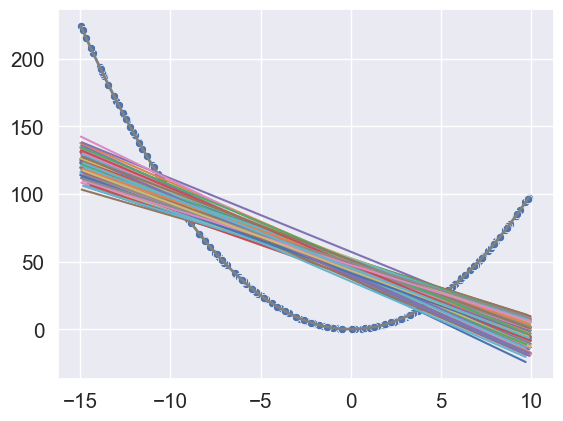
\includegraphics[keepaspectratio]{Bias_variance_code_files/figure-pdf/cell-4-output-1.png}}

The above plots show that the 100 models seem to have low variance, but
high bias. Note that the bias is low only around a couple of points
\emph{(x = -10 \& x = 5)}.

Let us compute the average squared bias over all the test data points.

\begin{Shaded}
\begin{Highlighting}[]
\NormalTok{mean\_pred }\OperatorTok{=}\NormalTok{ np.array(pred\_test).mean(axis }\OperatorTok{=} \DecValTok{0}\NormalTok{)}
\NormalTok{sq\_bias }\OperatorTok{=}\NormalTok{ ((mean\_pred }\OperatorTok{{-}}\NormalTok{ fxtest)}\OperatorTok{**}\DecValTok{2}\NormalTok{).mean()}
\NormalTok{sq\_bias}
\end{Highlighting}
\end{Shaded}

\begin{verbatim}
2042.104126728109
\end{verbatim}

Let us compute the average variance over all the test data points.

\begin{Shaded}
\begin{Highlighting}[]
\NormalTok{mean\_var }\OperatorTok{=}\NormalTok{ np.array(pred\_test).var(axis }\OperatorTok{=} \DecValTok{0}\NormalTok{).mean()}
\NormalTok{mean\_var}
\end{Highlighting}
\end{Shaded}

\begin{verbatim}
28.37397844429763
\end{verbatim}

Let us compute the mean squared error over all the test data points.

\begin{Shaded}
\begin{Highlighting}[]
\NormalTok{np.array(mse\_test).mean()}
\end{Highlighting}
\end{Shaded}

\begin{verbatim}
2070.4781051724062
\end{verbatim}

Note that the mean squared error should be the same as the sum of
squared bias and variance

The sum of squared bias and model variance is:

\begin{Shaded}
\begin{Highlighting}[]
\NormalTok{sq\_bias }\OperatorTok{+}\NormalTok{ mean\_var}
\end{Highlighting}
\end{Shaded}

\begin{verbatim}
2070.4781051724067
\end{verbatim}

Note that this is exactly the same as the mean squared error computed
above as we are developing a finite number of models, and making
predictions on a finite number of test data points.

\section{Complex model (more
flexible)}\label{complex-model-more-flexible}

Let us consider a decion tree as the more flexible model.

\begin{Shaded}
\begin{Highlighting}[]
\NormalTok{np.random.seed(}\DecValTok{101}\NormalTok{)}
\NormalTok{xtest }\OperatorTok{=}\NormalTok{ np.random.uniform(}\OperatorTok{{-}}\DecValTok{15}\NormalTok{, }\DecValTok{10}\NormalTok{, }\DecValTok{200}\NormalTok{)}
\NormalTok{fxtest }\OperatorTok{=}\NormalTok{ xtest}\OperatorTok{**}\DecValTok{2}
\NormalTok{ytest }\OperatorTok{=}\NormalTok{ fxtest}
\NormalTok{model }\OperatorTok{=}\NormalTok{ DecisionTreeRegressor()}
\end{Highlighting}
\end{Shaded}

\begin{Shaded}
\begin{Highlighting}[]
\NormalTok{sns.scatterplot(x }\OperatorTok{=}\NormalTok{ xtest, y }\OperatorTok{=}\NormalTok{ ytest)}
\NormalTok{sns.lineplot(x }\OperatorTok{=}\NormalTok{ xtest, y }\OperatorTok{=}\NormalTok{ fxtest, color }\OperatorTok{=} \StringTok{\textquotesingle{}grey\textquotesingle{}}\NormalTok{, linewidth }\OperatorTok{=} \DecValTok{2}\NormalTok{)}
\NormalTok{pred\_test }\OperatorTok{=}\NormalTok{ []}\OperatorTok{;}\NormalTok{ mse\_test }\OperatorTok{=}\NormalTok{ []}
\ControlFlowTok{for}\NormalTok{ i }\KeywordTok{in} \BuiltInTok{range}\NormalTok{(}\DecValTok{100}\NormalTok{):}
\NormalTok{    np.random.seed(i)}
\NormalTok{    x }\OperatorTok{=}\NormalTok{ np.random.uniform(}\OperatorTok{{-}}\DecValTok{15}\NormalTok{, }\DecValTok{10}\NormalTok{, }\DecValTok{200}\NormalTok{)}
\NormalTok{    fx }\OperatorTok{=}\NormalTok{ x}\OperatorTok{**}\DecValTok{2}
\NormalTok{    y }\OperatorTok{=}\NormalTok{ fx }\OperatorTok{+}\NormalTok{ np.random.normal(}\DecValTok{0}\NormalTok{, }\DecValTok{10}\NormalTok{, }\DecValTok{200}\NormalTok{)}
\NormalTok{    model.fit(x.reshape(}\OperatorTok{{-}}\DecValTok{1}\NormalTok{,}\DecValTok{1}\NormalTok{), y)}
\NormalTok{    sns.lineplot(x }\OperatorTok{=}\NormalTok{ x, y }\OperatorTok{=}\NormalTok{ model.predict(x.reshape(}\OperatorTok{{-}}\DecValTok{1}\NormalTok{,}\DecValTok{1}\NormalTok{)))}
\NormalTok{    pred\_test.append(model.predict(xtest.reshape(}\OperatorTok{{-}}\DecValTok{1}\NormalTok{,}\DecValTok{1}\NormalTok{)))}
\NormalTok{    mse\_test.append(mean\_squared\_error(model.predict(xtest.reshape(}\OperatorTok{{-}}\DecValTok{1}\NormalTok{,}\DecValTok{1}\NormalTok{)), ytest))}
\end{Highlighting}
\end{Shaded}

\pandocbounded{\includegraphics[keepaspectratio]{Bias_variance_code_files/figure-pdf/cell-10-output-1.png}}

The above plots show that the 100 models seem to have high variance, but
low bias.

Let us compute the average squared bias over all the test data points.

\begin{Shaded}
\begin{Highlighting}[]
\NormalTok{mean\_pred }\OperatorTok{=}\NormalTok{ np.array(pred\_test).mean(axis }\OperatorTok{=} \DecValTok{0}\NormalTok{)}
\NormalTok{sq\_bias }\OperatorTok{=}\NormalTok{ ((mean\_pred }\OperatorTok{{-}}\NormalTok{ fxtest)}\OperatorTok{**}\DecValTok{2}\NormalTok{).mean()}
\NormalTok{sq\_bias}
\end{Highlighting}
\end{Shaded}

\begin{verbatim}
1.3117561629333938
\end{verbatim}

Let us compute the average model variance over all the test data points.

\begin{Shaded}
\begin{Highlighting}[]
\NormalTok{mean\_var }\OperatorTok{=}\NormalTok{ np.array(pred\_test).var(axis }\OperatorTok{=} \DecValTok{0}\NormalTok{).mean()}
\NormalTok{mean\_var}
\end{Highlighting}
\end{Shaded}

\begin{verbatim}
102.5226748977198
\end{verbatim}

Let us compute the average mean squared error over all the test data
points.

\begin{Shaded}
\begin{Highlighting}[]
\NormalTok{np.array(mse\_test).mean()}
\end{Highlighting}
\end{Shaded}

\begin{verbatim}
103.83443106065317
\end{verbatim}

Note that the above error is still the same as the sum of the squared
bias, model variance and the irreducible error.

Note that the relatively more flexible model has a higher variance, but
lower bias as compared to the less flexible linear model. This will
typically be the case, but may not be true in all scenarios. We will
discuss one such scenario later.

\chapter{KNN}\label{knn}

\emph{Read section 4.7.6 of the book before using these notes.}

\emph{Note that in this course, lecture notes are not sufficient, you
must read the book for better understanding. Lecture notes are just
implementing the concepts of the book on a dataset, but not explaining
the concepts elaborately.}

\begin{Shaded}
\begin{Highlighting}[]
\CommentTok{\# Importing necessary libraries}
\ImportTok{import}\NormalTok{ pandas }\ImportTok{as}\NormalTok{ pd}
\ImportTok{import}\NormalTok{ numpy }\ImportTok{as}\NormalTok{ np}
\ImportTok{import}\NormalTok{ matplotlib.pyplot }\ImportTok{as}\NormalTok{ plt}
\ImportTok{import}\NormalTok{ seaborn }\ImportTok{as}\NormalTok{ sns}
\NormalTok{sns.}\BuiltInTok{set}\NormalTok{(font\_scale}\OperatorTok{=}\FloatTok{1.35}\NormalTok{)}

\ImportTok{from}\NormalTok{ sklearn.preprocessing }\ImportTok{import}\NormalTok{ StandardScaler}
\ImportTok{from}\NormalTok{ sklearn.neighbors }\ImportTok{import}\NormalTok{ KNeighborsRegressor, KNeighborsClassifier}
\ImportTok{from}\NormalTok{ sklearn.model\_selection }\ImportTok{import}\NormalTok{ cross\_val\_score, GridSearchCV, cross\_val\_predict, KFold, RepeatedKFold}

\ImportTok{from}\NormalTok{ sklearn.pipeline }\ImportTok{import}\NormalTok{ Pipeline}
\ImportTok{from}\NormalTok{ sklearn.compose }\ImportTok{import}\NormalTok{ ColumnTransformer}
\ImportTok{from}\NormalTok{ sklearn.preprocessing }\ImportTok{import}\NormalTok{ OneHotEncoder, FunctionTransformer}
\ImportTok{from}\NormalTok{ sklearn.metrics }\ImportTok{import}\NormalTok{ root\_mean\_squared\_error, r2\_score}
\end{Highlighting}
\end{Shaded}

\section{KNN for regression}\label{knn-for-regression}

\begin{Shaded}
\begin{Highlighting}[]
\CommentTok{\# Load the dataset}
\NormalTok{car }\OperatorTok{=}\NormalTok{ pd.read\_csv(}\StringTok{\textquotesingle{}Datasets/car.csv\textquotesingle{}}\NormalTok{)}

\CommentTok{\# Split the dataset into features and target variable}
\NormalTok{X }\OperatorTok{=}\NormalTok{ car.drop(columns}\OperatorTok{=}\NormalTok{[}\StringTok{\textquotesingle{}price\textquotesingle{}}\NormalTok{])}
\NormalTok{y }\OperatorTok{=}\NormalTok{ car[}\StringTok{\textquotesingle{}price\textquotesingle{}}\NormalTok{]}

\CommentTok{\# split the dataset into training and testing sets}
\ImportTok{from}\NormalTok{ sklearn.model\_selection }\ImportTok{import}\NormalTok{ train\_test\_split}
\NormalTok{X\_train, X\_test, y\_train, y\_test }\OperatorTok{=}\NormalTok{ train\_test\_split(X, y, test\_size}\OperatorTok{=}\FloatTok{0.2}\NormalTok{, random\_state}\OperatorTok{=}\DecValTok{42}\NormalTok{)}
\end{Highlighting}
\end{Shaded}

\begin{Shaded}
\begin{Highlighting}[]
\CommentTok{\# extract the categorical columns and put them in a list}
\NormalTok{cat\_cols }\OperatorTok{=}\NormalTok{ X.select\_dtypes(include}\OperatorTok{=}\NormalTok{[}\StringTok{\textquotesingle{}object\textquotesingle{}}\NormalTok{]).columns.tolist()}

\CommentTok{\# extract the numerical columns and put them in a list}
\NormalTok{num\_cols }\OperatorTok{=}\NormalTok{ X.select\_dtypes(include}\OperatorTok{=}\NormalTok{[}\StringTok{\textquotesingle{}int64\textquotesingle{}}\NormalTok{, }\StringTok{\textquotesingle{}float64\textquotesingle{}}\NormalTok{]).columns.tolist()}
\end{Highlighting}
\end{Shaded}

\begin{Shaded}
\begin{Highlighting}[]
\CommentTok{\# First transform categorical variables}
\NormalTok{preprocessor }\OperatorTok{=}\NormalTok{ ColumnTransformer(}
\NormalTok{    transformers}\OperatorTok{=}\NormalTok{[}
\NormalTok{        (}\StringTok{\textquotesingle{}num\textquotesingle{}}\NormalTok{, }\StringTok{\textquotesingle{}passthrough\textquotesingle{}}\NormalTok{, num\_cols),  }\CommentTok{\# Just pass numerical features through}
\NormalTok{        (}\StringTok{\textquotesingle{}cat\textquotesingle{}}\NormalTok{, OneHotEncoder(handle\_unknown}\OperatorTok{=}\StringTok{\textquotesingle{}ignore\textquotesingle{}}\NormalTok{, sparse\_output}\OperatorTok{=}\VariableTok{False}\NormalTok{), cat\_cols)}
\NormalTok{    ])}

\CommentTok{\# Create pipeline that scales all features together}
\NormalTok{pipeline }\OperatorTok{=}\NormalTok{ Pipeline(steps}\OperatorTok{=}\NormalTok{[}
\NormalTok{    (}\StringTok{\textquotesingle{}preprocessor\textquotesingle{}}\NormalTok{, preprocessor),}
\NormalTok{    (}\StringTok{\textquotesingle{}scaler\textquotesingle{}}\NormalTok{, StandardScaler()),  }\CommentTok{\# Scale everything together}
\NormalTok{    (}\StringTok{\textquotesingle{}knn\textquotesingle{}}\NormalTok{, KNeighborsRegressor(n\_neighbors}\OperatorTok{=}\DecValTok{5}\NormalTok{))}
\NormalTok{])}

\CommentTok{\# Fit the pipeline to the training data}
\NormalTok{pipeline.fit(X\_train, y\_train)}
\CommentTok{\# Predict on the test data}
\NormalTok{y\_pred }\OperatorTok{=}\NormalTok{ pipeline.predict(X\_test)}
\CommentTok{\# Calculate RMSE}
\NormalTok{rmse }\OperatorTok{=}\NormalTok{ root\_mean\_squared\_error(y\_test, y\_pred)}
\BuiltInTok{print}\NormalTok{(}\SpecialStringTok{f"RMSE: }\SpecialCharTok{\{}\NormalTok{rmse}\SpecialCharTok{:.2f\}}\SpecialStringTok{"}\NormalTok{)}
\BuiltInTok{print}\NormalTok{(}\SpecialStringTok{f"R² Score: }\SpecialCharTok{\{}\NormalTok{pipeline}\SpecialCharTok{.}\NormalTok{score(X\_test, y\_test)}\SpecialCharTok{:.2f\}}\SpecialStringTok{"}\NormalTok{)}
\end{Highlighting}
\end{Shaded}

\begin{verbatim}
RMSE: 4364.84
R² Score: 0.94
\end{verbatim}

\begin{Shaded}
\begin{Highlighting}[]
\CommentTok{\# show the features in the numerical transformer    }
\NormalTok{pipeline.named\_steps[}\StringTok{\textquotesingle{}preprocessor\textquotesingle{}}\NormalTok{].transformers\_[}\DecValTok{0}\NormalTok{][}\DecValTok{1}\NormalTok{].get\_feature\_names\_out()}
\BuiltInTok{print}\NormalTok{(}\StringTok{"numerical features in the pipeline:"}\NormalTok{, pipeline.named\_steps[}\StringTok{\textquotesingle{}preprocessor\textquotesingle{}}\NormalTok{].transformers\_[}\DecValTok{0}\NormalTok{][}\DecValTok{1}\NormalTok{].get\_feature\_names\_out())}

\CommentTok{\# show the features in the categorical transformer}
\NormalTok{pipeline.named\_steps[}\StringTok{\textquotesingle{}preprocessor\textquotesingle{}}\NormalTok{].transformers\_[}\DecValTok{1}\NormalTok{][}\DecValTok{1}\NormalTok{].get\_feature\_names\_out()}
\BuiltInTok{print}\NormalTok{(}\StringTok{"categorical features in the pipeline:"}\NormalTok{, pipeline.named\_steps[}\StringTok{\textquotesingle{}preprocessor\textquotesingle{}}\NormalTok{].transformers\_[}\DecValTok{1}\NormalTok{][}\DecValTok{1}\NormalTok{].get\_feature\_names\_out())}
\end{Highlighting}
\end{Shaded}

\begin{verbatim}
numerical features in the pipeline: ['year' 'mileage' 'tax' 'mpg' 'engineSize']
categorical features in the pipeline: ['brand_audi' 'brand_bmw' 'brand_ford' 'brand_hyundi' 'brand_merc'
 'brand_skoda' 'brand_toyota' 'brand_vauxhall' 'brand_vw'
 'model_ 6 Series' 'model_ 7 Series' 'model_ 8 Series' 'model_ A7'
 'model_ A8' 'model_ Agila' 'model_ Amarok' 'model_ Antara'
 'model_ Arteon' 'model_ Avensis' 'model_ Beetle' 'model_ CC'
 'model_ CLA Class' 'model_ CLK' 'model_ CLS Class' 'model_ Caddy'
 'model_ Caddy Life' 'model_ Caddy Maxi Life' 'model_ California'
 'model_ Camry' 'model_ Caravelle' 'model_ Combo Life' 'model_ Edge'
 'model_ Eos' 'model_ Fusion' 'model_ G Class' 'model_ GL Class'
 'model_ GLB Class' 'model_ GLS Class' 'model_ GT86' 'model_ GTC'
 'model_ Galaxy' 'model_ Getz' 'model_ Grand C-MAX'
 'model_ Grand Tourneo Connect' 'model_ Hilux' 'model_ I40' 'model_ I800'
 'model_ IQ' 'model_ IX20' 'model_ IX35' 'model_ Jetta' 'model_ KA'
 'model_ Kamiq' 'model_ Land Cruiser' 'model_ M Class' 'model_ M2'
 'model_ M3' 'model_ M4' 'model_ M5' 'model_ M6' 'model_ Mustang'
 'model_ PROACE VERSO' 'model_ Prius' 'model_ Puma' 'model_ Q8'
 'model_ R8' 'model_ RS3' 'model_ RS4' 'model_ RS5' 'model_ RS6'
 'model_ Rapid' 'model_ Roomster' 'model_ S Class' 'model_ S3' 'model_ S4'
 'model_ SLK' 'model_ SQ5' 'model_ SQ7' 'model_ Santa Fe' 'model_ Scala'
 'model_ Scirocco' 'model_ Shuttle' 'model_ Supra'
 'model_ Tiguan Allspace' 'model_ Tourneo Connect' 'model_ Tourneo Custom'
 'model_ V Class' 'model_ Verso' 'model_ Vivaro' 'model_ X-CLASS'
 'model_ X4' 'model_ X6' 'model_ X7' 'model_ Yeti' 'model_ Z3' 'model_ Z4'
 'model_ Zafira Tourer' 'model_ i3' 'model_ i8' 'transmission_Automatic'
 'transmission_Manual' 'transmission_Other' 'transmission_Semi-Auto'
 'fuelType_Diesel' 'fuelType_Electric' 'fuelType_Hybrid' 'fuelType_Other'
 'fuelType_Petrol']
\end{verbatim}

\section{Feature Scaling in KNN}\label{feature-scaling-in-knn}

\textbf{Feature scaling is essential when using K-Nearest Neighbors
(KNN)} because the algorithm relies on calculating distances between
data points. If features are measured on different scales (e.g.,
\texttt{mileage} in thousands and \texttt{mpg} in tens), the features
with larger numeric ranges can dominate the distance calculations and
distort the results.

To ensure that all features contribute equally, it's important to
\textbf{standardize or normalize} them before applying KNN. Common
scaling techniques include:

\begin{itemize}
\tightlist
\item
  \textbf{Standardization} (zero mean, unit variance) using
  \texttt{StandardScaler}
\item
  \textbf{Min-max scaling} to bring values into the \texttt{{[}0,\ 1{]}}
  range
\end{itemize}

Without scaling, KNN may produce biased or misleading predictions.\\
The example below illustrates how the same KNN model performs
\textbf{without feature scaling}, highlighting the importance of
preprocessing your data.

\begin{Shaded}
\begin{Highlighting}[]
\NormalTok{preprocessor\_no\_scaling }\OperatorTok{=}\NormalTok{ ColumnTransformer(}
\NormalTok{    transformers}\OperatorTok{=}\NormalTok{[}
\NormalTok{        (}\StringTok{\textquotesingle{}num\textquotesingle{}}\NormalTok{, }\StringTok{\textquotesingle{}passthrough\textquotesingle{}}\NormalTok{, num\_cols),  }\CommentTok{\# Pass numerical features through without scaling}
\NormalTok{        (}\StringTok{\textquotesingle{}cat\textquotesingle{}}\NormalTok{, OneHotEncoder(handle\_unknown}\OperatorTok{=}\StringTok{\textquotesingle{}ignore\textquotesingle{}}\NormalTok{), cat\_cols)  }\CommentTok{\# Only one{-}hot encode categorical}
\NormalTok{    ])}

\CommentTok{\# Create pipeline without any scaling}
\NormalTok{pipeline\_no\_scaling }\OperatorTok{=}\NormalTok{ Pipeline(steps}\OperatorTok{=}\NormalTok{[}
\NormalTok{    (}\StringTok{\textquotesingle{}preprocessor\textquotesingle{}}\NormalTok{, preprocessor\_no\_scaling),}
\NormalTok{    (}\StringTok{\textquotesingle{}knn\textquotesingle{}}\NormalTok{, KNeighborsRegressor(n\_neighbors}\OperatorTok{=}\DecValTok{5}\NormalTok{))}
\NormalTok{])}

\CommentTok{\# Fit the pipeline}
\NormalTok{pipeline\_no\_scaling.fit(X\_train, y\_train)}

\CommentTok{\# Evaluate}
\NormalTok{y\_pred\_no\_scaling }\OperatorTok{=}\NormalTok{ pipeline\_no\_scaling.predict(X\_test)}

\NormalTok{rmse\_no\_scaling }\OperatorTok{=}\NormalTok{ root\_mean\_squared\_error(y\_test, y\_pred\_no\_scaling)}
\BuiltInTok{print}\NormalTok{(}\SpecialStringTok{f"RMSE without scaling: }\SpecialCharTok{\{}\NormalTok{rmse\_no\_scaling}\SpecialCharTok{:.2f\}}\SpecialStringTok{"}\NormalTok{)}
\BuiltInTok{print}\NormalTok{(}\SpecialStringTok{f"R² Score without scaling: }\SpecialCharTok{\{}\NormalTok{pipeline\_no\_scaling}\SpecialCharTok{.}\NormalTok{score(X\_test, y\_test)}\SpecialCharTok{:.2f\}}\SpecialStringTok{"}\NormalTok{)}
\end{Highlighting}
\end{Shaded}

\begin{verbatim}
RMSE without scaling: 13758.38
R² Score without scaling: 0.35
\end{verbatim}

\section{Hyperparameters in KNN}\label{hyperparameters-in-knn}

The most important hyperparameter in K-Nearest Neighbors (KNN) is
\textbf{\emph{k}}, which determines the number of neighbors considered
when making predictions. Tuning \emph{k} helps balance the model's
\textbf{bias and variance}:

\begin{itemize}
\tightlist
\item
  A \textbf{small \emph{k}} (e.g., 1 or 3) can lead to \textbf{low bias
  but high variance}, making the model sensitive to noise in the
  training data.
\item
  A \textbf{large \emph{k}} results in \textbf{higher bias but lower
  variance}, producing smoother predictions that may underfit the data.
\end{itemize}

\subsection{\texorpdfstring{Tuning \emph{k} in
KNN}{Tuning k in KNN}}\label{tuning-k-in-knn}

To find the optimal value of \emph{k}, it's common to use
\textbf{cross-validation}, which evaluates model performance on
different subsets of the data. A popular tool for this is
\textbf{\texttt{GridSearchCV}}, which automates the search process by
testing multiple values of \emph{k} using cross-validation behind the
scenes. It selects the value of \emph{k} that minimizes prediction error
on unseen data---helping you achieve a good balance between underfitting
and overfitting.

\begin{Shaded}
\begin{Highlighting}[]
\CommentTok{\# Create parameter grid for k values}
\NormalTok{param\_grid }\OperatorTok{=}\NormalTok{ \{}
    \StringTok{\textquotesingle{}knn\_\_n\_neighbors\textquotesingle{}}\NormalTok{: }\BuiltInTok{list}\NormalTok{(}\BuiltInTok{range}\NormalTok{(}\DecValTok{1}\NormalTok{, }\DecValTok{20}\NormalTok{))  }\CommentTok{\# Test k values from 1 to 20}
\NormalTok{\}}

\CommentTok{\# Set up GridSearchCV}
\NormalTok{grid\_search }\OperatorTok{=}\NormalTok{ GridSearchCV(}
\NormalTok{    estimator}\OperatorTok{=}\NormalTok{pipeline,}
\NormalTok{    param\_grid}\OperatorTok{=}\NormalTok{param\_grid,}
\NormalTok{    cv}\OperatorTok{=}\DecValTok{5}\NormalTok{,  }\CommentTok{\# 5{-}fold cross{-}validation}
\NormalTok{    scoring}\OperatorTok{=}\StringTok{\textquotesingle{}neg\_root\_mean\_squared\_error\textquotesingle{}}\NormalTok{,  }\CommentTok{\# Optimize for RMSE}
\NormalTok{    n\_jobs}\OperatorTok{={-}}\DecValTok{1}\NormalTok{,  }\CommentTok{\# Use all available cores}
\NormalTok{    verbose}\OperatorTok{=}\DecValTok{1}
\NormalTok{)}

\CommentTok{\# Fit grid search}
\BuiltInTok{print}\NormalTok{(}\StringTok{"Tuning k parameter..."}\NormalTok{)}
\NormalTok{grid\_search.fit(X\_train, y\_train)}

\CommentTok{\# Get best parameters and results}
\NormalTok{best\_k }\OperatorTok{=}\NormalTok{ grid\_search.best\_params\_[}\StringTok{\textquotesingle{}knn\_\_n\_neighbors\textquotesingle{}}\NormalTok{]}
\NormalTok{best\_score }\OperatorTok{=} \OperatorTok{{-}}\NormalTok{grid\_search.best\_score\_  }\CommentTok{\# Convert back from negative RMSE}

\BuiltInTok{print}\NormalTok{(}\SpecialStringTok{f"Best k: }\SpecialCharTok{\{}\NormalTok{best\_k}\SpecialCharTok{\}}\SpecialStringTok{"}\NormalTok{)}
\BuiltInTok{print}\NormalTok{(}\SpecialStringTok{f"Best CV RMSE: }\SpecialCharTok{\{}\NormalTok{best\_score}\SpecialCharTok{:.2f\}}\SpecialStringTok{"}\NormalTok{)}

\CommentTok{\# Evaluate on test set using best model}
\NormalTok{best\_model }\OperatorTok{=}\NormalTok{ grid\_search.best\_estimator\_}
\NormalTok{y\_pred }\OperatorTok{=}\NormalTok{ best\_model.predict(X\_test)}
\NormalTok{test\_rmse }\OperatorTok{=}\NormalTok{ root\_mean\_squared\_error(y\_test, y\_pred)}
\NormalTok{test\_r2 }\OperatorTok{=}\NormalTok{ r2\_score(y\_test, y\_pred)}

\BuiltInTok{print}\NormalTok{(}\SpecialStringTok{f"Test RMSE with k=}\SpecialCharTok{\{}\NormalTok{best\_k}\SpecialCharTok{\}}\SpecialStringTok{: }\SpecialCharTok{\{}\NormalTok{test\_rmse}\SpecialCharTok{:.2f\}}\SpecialStringTok{"}\NormalTok{)}
\BuiltInTok{print}\NormalTok{(}\SpecialStringTok{f"Test R² Score with k=}\SpecialCharTok{\{}\NormalTok{best\_k}\SpecialCharTok{\}}\SpecialStringTok{: }\SpecialCharTok{\{}\NormalTok{test\_r2}\SpecialCharTok{:.2f\}}\SpecialStringTok{"}\NormalTok{)}
\end{Highlighting}
\end{Shaded}

\begin{verbatim}
Tuning k parameter...
Fitting 5 folds for each of 19 candidates, totalling 95 fits
Best k: 3
Best CV RMSE: 4117.42
Test RMSE with k=3: 4051.06
Test R² Score with k=3: 0.94
\end{verbatim}

\begin{Shaded}
\begin{Highlighting}[]
\CommentTok{\# Plot performance across different k values}
\NormalTok{cv\_results }\OperatorTok{=}\NormalTok{ grid\_search.cv\_results\_}
\NormalTok{k\_values }\OperatorTok{=}\NormalTok{ param\_grid[}\StringTok{\textquotesingle{}knn\_\_n\_neighbors\textquotesingle{}}\NormalTok{]}
\NormalTok{mean\_rmse }\OperatorTok{=} \OperatorTok{{-}}\NormalTok{cv\_results[}\StringTok{\textquotesingle{}mean\_test\_score\textquotesingle{}}\NormalTok{] }

\NormalTok{plt.figure(figsize}\OperatorTok{=}\NormalTok{(}\DecValTok{10}\NormalTok{, }\DecValTok{6}\NormalTok{))}
\NormalTok{plt.plot(k\_values, mean\_rmse, marker}\OperatorTok{=}\StringTok{\textquotesingle{}o\textquotesingle{}}\NormalTok{)}
\NormalTok{plt.xlabel(}\StringTok{\textquotesingle{}k (Number of Neighbors)\textquotesingle{}}\NormalTok{)}
\NormalTok{plt.ylabel(}\StringTok{\textquotesingle{}RMSE (Cross{-}Validation)\textquotesingle{}}\NormalTok{)}
\NormalTok{plt.title(}\StringTok{\textquotesingle{}KNN Performance for Different k Values\textquotesingle{}}\NormalTok{)}
\NormalTok{plt.grid(}\VariableTok{True}\NormalTok{)}
\NormalTok{plt.xticks(k\_values)}
\NormalTok{plt.axvline(x}\OperatorTok{=}\NormalTok{best\_k, color}\OperatorTok{=}\StringTok{\textquotesingle{}r\textquotesingle{}}\NormalTok{, linestyle}\OperatorTok{=}\StringTok{\textquotesingle{}{-}{-}\textquotesingle{}}\NormalTok{, label}\OperatorTok{=}\SpecialStringTok{f\textquotesingle{}Best k = }\SpecialCharTok{\{}\NormalTok{best\_k}\SpecialCharTok{\}}\SpecialStringTok{\textquotesingle{}}\NormalTok{)}
\NormalTok{plt.legend()}
\NormalTok{plt.tight\_layout()}
\NormalTok{plt.show()}
\end{Highlighting}
\end{Shaded}

\pandocbounded{\includegraphics[keepaspectratio]{KNN_files/figure-pdf/cell-9-output-1.png}}

The distances and the indices of the nearest K observations to each test
observation can be obtained using the \texttt{kneighbors()} method.

\begin{Shaded}
\begin{Highlighting}[]
\CommentTok{\# Get the KNN estimator from the pipeline}
\NormalTok{knn\_estimator }\OperatorTok{=}\NormalTok{ best\_model.named\_steps[}\StringTok{\textquotesingle{}knn\textquotesingle{}}\NormalTok{]}

\CommentTok{\# Get indices of K{-}nearest neighbors for each test observation}
\NormalTok{neighbor\_indices }\OperatorTok{=}\NormalTok{ knn\_estimator.kneighbors(best\_model.named\_steps[}\StringTok{\textquotesingle{}preprocessor\textquotesingle{}}\NormalTok{].transform(X\_test), }
\NormalTok{                                           return\_distance}\OperatorTok{=}\VariableTok{False}\NormalTok{)}
\CommentTok{\# neighbor\_indices will contain the indices of the K nearest neighbors for each test observation}
\CommentTok{\# Note: The indices are relative to the training set, not the test set.}
\CommentTok{\# To get the actual neighbor observations, you can use these indices to index into the training set}
\CommentTok{\# For example, to get the actual neighbor observations for the first test observation:}
\NormalTok{neighbors }\OperatorTok{=}\NormalTok{ X\_train.iloc[neighbor\_indices[}\DecValTok{0}\NormalTok{]]}
\NormalTok{neighbors}
\end{Highlighting}
\end{Shaded}

\begin{longtable}[]{@{}llllllllll@{}}
\toprule\noalign{}
& brand & model & year & transmission & mileage & fuelType & tax & mpg &
engineSize \\
\midrule\noalign{}
\endhead
\bottomrule\noalign{}
\endlastfoot
4580 & merc & V Class & 2010 & Automatic & 259000 & Diesel & 540 &
30.8345 & 3.0 \\
5651 & merc & CLK & 2003 & Automatic & 185000 & Petrol & 330 & 18.0803 &
4.3 \\
3961 & vw & Caravelle & 2006 & Manual & 178000 & Diesel & 325 & 34.5738
& 2.5 \\
\end{longtable}

\subsection{Tuning Other KNN
Hyperparameters}\label{tuning-other-knn-hyperparameters}

In addition to the number of neighbors (\emph{k}), KNN has several other
important hyperparameters that can significantly affect the model's
performance. Fine-tuning these settings helps you get the most out of
the algorithm. Key hyperparameters include:

\begin{itemize}
\tightlist
\item
  \textbf{\texttt{weights}}: Determines how the neighbors contribute to
  the prediction.

  \begin{itemize}
  \tightlist
  \item
    \texttt{\textquotesingle{}uniform\textquotesingle{}}: All neighbors
    are weighted equally (default).\\
  \item
    \texttt{\textquotesingle{}distance\textquotesingle{}}: Closer
    neighbors have more influence.\\
  \item
    Choosing \texttt{\textquotesingle{}distance\textquotesingle{}} can
    improve performance, especially when data points are unevenly
    distributed.
  \end{itemize}
\item
  \textbf{\texttt{metric}}: Defines the distance function used to
  measure similarity between data points.

  \begin{itemize}
  \tightlist
  \item
    \texttt{\textquotesingle{}minkowski\textquotesingle{}} (default) is
    a general-purpose metric that includes both Euclidean and Manhattan
    distances.\\
  \item
    Other options include
    \texttt{\textquotesingle{}euclidean\textquotesingle{}},
    \texttt{\textquotesingle{}manhattan\textquotesingle{}}, or even
    custom distance functions.
  \end{itemize}
\item
  \textbf{\texttt{p}}: Used when
  \texttt{metric=\textquotesingle{}minkowski\textquotesingle{}}.

  \begin{itemize}
  \tightlist
  \item
    \texttt{p=2} gives \textbf{Euclidean distance} (standard for
    continuous features).\\
  \item
    \texttt{p=1} gives \textbf{Manhattan distance} (useful when features
    are sparse or grid-based).
  \end{itemize}
\item
  \textbf{\texttt{algorithm}}: Controls the method used to compute
  nearest neighbors.

  \begin{itemize}
  \tightlist
  \item
    \texttt{\textquotesingle{}auto\textquotesingle{}},
    \texttt{\textquotesingle{}ball\_tree\textquotesingle{}},
    \texttt{\textquotesingle{}kd\_tree\textquotesingle{}}, or
    \texttt{\textquotesingle{}brute\textquotesingle{}}.\\
  \item
    Most users can leave this as
    \texttt{\textquotesingle{}auto\textquotesingle{}}, which lets
    scikit-learn choose the best algorithm based on the data.
  \end{itemize}
\end{itemize}

These hyperparameters can be tuned using \texttt{GridSearchCV} to find
the combination that yields the best performance on validation data.

The model hyperparameters can be obtained using the
\texttt{get\_params()} method. Note that there are other hyperparameters
to tune in addition to number of neighbors. However, the number of
neighbours may be the most influential hyperparameter in most cases.

\begin{Shaded}
\begin{Highlighting}[]
\CommentTok{\# Get the best model parameters}
\NormalTok{best\_model.get\_params()}
\end{Highlighting}
\end{Shaded}

\begin{verbatim}
{'memory': None,
 'steps': [('preprocessor',
   ColumnTransformer(transformers=[('num', 'passthrough',
                                    ['year', 'mileage', 'tax', 'mpg',
                                     'engineSize']),
                                   ('cat',
                                    OneHotEncoder(handle_unknown='ignore',
                                                  sparse_output=False),
                                    ['brand', 'model', 'transmission',
                                     'fuelType'])])),
  ('scaler', StandardScaler()),
  ('knn', KNeighborsRegressor(n_neighbors=3))],
 'transform_input': None,
 'verbose': False,
 'preprocessor': ColumnTransformer(transformers=[('num', 'passthrough',
                                  ['year', 'mileage', 'tax', 'mpg',
                                   'engineSize']),
                                 ('cat',
                                  OneHotEncoder(handle_unknown='ignore',
                                                sparse_output=False),
                                  ['brand', 'model', 'transmission',
                                   'fuelType'])]),
 'scaler': StandardScaler(),
 'knn': KNeighborsRegressor(n_neighbors=3),
 'preprocessor__force_int_remainder_cols': True,
 'preprocessor__n_jobs': None,
 'preprocessor__remainder': 'drop',
 'preprocessor__sparse_threshold': 0.3,
 'preprocessor__transformer_weights': None,
 'preprocessor__transformers': [('num',
   'passthrough',
   ['year', 'mileage', 'tax', 'mpg', 'engineSize']),
  ('cat',
   OneHotEncoder(handle_unknown='ignore', sparse_output=False),
   ['brand', 'model', 'transmission', 'fuelType'])],
 'preprocessor__verbose': False,
 'preprocessor__verbose_feature_names_out': True,
 'preprocessor__num': 'passthrough',
 'preprocessor__cat': OneHotEncoder(handle_unknown='ignore', sparse_output=False),
 'preprocessor__cat__categories': 'auto',
 'preprocessor__cat__drop': None,
 'preprocessor__cat__dtype': numpy.float64,
 'preprocessor__cat__feature_name_combiner': 'concat',
 'preprocessor__cat__handle_unknown': 'ignore',
 'preprocessor__cat__max_categories': None,
 'preprocessor__cat__min_frequency': None,
 'preprocessor__cat__sparse_output': False,
 'scaler__copy': True,
 'scaler__with_mean': True,
 'scaler__with_std': True,
 'knn__algorithm': 'auto',
 'knn__leaf_size': 30,
 'knn__metric': 'minkowski',
 'knn__metric_params': None,
 'knn__n_jobs': None,
 'knn__n_neighbors': 3,
 'knn__p': 2,
 'knn__weights': 'uniform'}
\end{verbatim}

\begin{Shaded}
\begin{Highlighting}[]
\CommentTok{\# Extended parameter grid}
\NormalTok{param\_grid }\OperatorTok{=}\NormalTok{ \{}
    \StringTok{\textquotesingle{}knn\_\_n\_neighbors\textquotesingle{}}\NormalTok{: }\BuiltInTok{list}\NormalTok{(}\BuiltInTok{range}\NormalTok{(}\DecValTok{1}\NormalTok{, }\DecValTok{20}\NormalTok{, }\DecValTok{2}\NormalTok{)),  }\CommentTok{\# Test odd k values from 1 to 19 (step=2 for efficiency)}
    \StringTok{\textquotesingle{}knn\_\_weights\textquotesingle{}}\NormalTok{: [}\StringTok{\textquotesingle{}uniform\textquotesingle{}}\NormalTok{, }\StringTok{\textquotesingle{}distance\textquotesingle{}}\NormalTok{],  }\CommentTok{\# Uniform: equal weight; Distance: closer neighbors weigh more}
    \StringTok{\textquotesingle{}knn\_\_metric\textquotesingle{}}\NormalTok{: [}\StringTok{\textquotesingle{}euclidean\textquotesingle{}}\NormalTok{, }\StringTok{\textquotesingle{}manhattan\textquotesingle{}}\NormalTok{, }\StringTok{\textquotesingle{}minkowski\textquotesingle{}}\NormalTok{],  }\CommentTok{\# Common distance metrics}
    \StringTok{\textquotesingle{}knn\_\_p\textquotesingle{}}\NormalTok{: [}\DecValTok{1}\NormalTok{, }\DecValTok{2}\NormalTok{]  }\CommentTok{\# p=1 (Manhattan), p=2 (Euclidean) {-} only relevant for Minkowski}
\NormalTok{\}}

\CommentTok{\# Set up GridSearchCV}
\NormalTok{grid\_search }\OperatorTok{=}\NormalTok{ GridSearchCV(}
\NormalTok{    estimator}\OperatorTok{=}\NormalTok{pipeline,}
\NormalTok{    param\_grid}\OperatorTok{=}\NormalTok{param\_grid,}
\NormalTok{    cv}\OperatorTok{=}\DecValTok{5}\NormalTok{,  }\CommentTok{\# 5{-}fold cross{-}validation}
\NormalTok{    scoring}\OperatorTok{=}\StringTok{\textquotesingle{}neg\_root\_mean\_squared\_error\textquotesingle{}}\NormalTok{,  }\CommentTok{\# Optimize for RMSE}
\NormalTok{    n\_jobs}\OperatorTok{={-}}\DecValTok{1}\NormalTok{,  }\CommentTok{\# Use all available cores}
\NormalTok{    verbose}\OperatorTok{=}\DecValTok{1}
\NormalTok{)}

\CommentTok{\# Fit grid search}
\BuiltInTok{print}\NormalTok{(}\StringTok{"Tuning KNN hyperparameters..."}\NormalTok{)}
\NormalTok{grid\_search.fit(X\_train, y\_train)}

\CommentTok{\# Get best parameters and results}
\NormalTok{best\_params }\OperatorTok{=}\NormalTok{ grid\_search.best\_params\_}
\NormalTok{best\_score }\OperatorTok{=} \OperatorTok{{-}}\NormalTok{grid\_search.best\_score\_  }\CommentTok{\# Convert negative RMSE to positive}

\CommentTok{\# Display results}
\BuiltInTok{print}\NormalTok{(}\StringTok{"}\CharTok{\textbackslash{}n}\StringTok{Best Parameters:"}\NormalTok{)}
\ControlFlowTok{for}\NormalTok{ param, value }\KeywordTok{in}\NormalTok{ best\_params.items():}
    \BuiltInTok{print}\NormalTok{(}\SpecialStringTok{f"}\SpecialCharTok{\{}\NormalTok{param}\SpecialCharTok{\}}\SpecialStringTok{: }\SpecialCharTok{\{}\NormalTok{value}\SpecialCharTok{\}}\SpecialStringTok{"}\NormalTok{)}
\BuiltInTok{print}\NormalTok{(}\SpecialStringTok{f"Best CV RMSE: }\SpecialCharTok{\{}\NormalTok{best\_score}\SpecialCharTok{:.2f\}}\SpecialStringTok{"}\NormalTok{)}

\CommentTok{\# Evaluate on test set using best model}
\NormalTok{best\_model }\OperatorTok{=}\NormalTok{ grid\_search.best\_estimator\_}
\NormalTok{y\_pred }\OperatorTok{=}\NormalTok{ best\_model.predict(X\_test)}
\NormalTok{test\_rmse }\OperatorTok{=}\NormalTok{ root\_mean\_squared\_error(y\_test, y\_pred)  }\CommentTok{\# Calculate RMSE}
\BuiltInTok{print}\NormalTok{(}\SpecialStringTok{f"Test RMSE: }\SpecialCharTok{\{}\NormalTok{test\_rmse}\SpecialCharTok{:.2f\}}\SpecialStringTok{"}\NormalTok{)}
\end{Highlighting}
\end{Shaded}

\begin{verbatim}
Tuning KNN hyperparameters...
Fitting 5 folds for each of 120 candidates, totalling 600 fits

Best Parameters:
knn__metric: euclidean
knn__n_neighbors: 3
knn__p: 1
knn__weights: distance
Best CV RMSE: 4001.34
Test RMSE: 3826.94
\end{verbatim}

The results for each cross-validation are stored in the
\texttt{cv\_results\_} attribute.

\begin{Shaded}
\begin{Highlighting}[]
\NormalTok{pd.DataFrame(grid\_search.cv\_results\_).head()}
\end{Highlighting}
\end{Shaded}

\begin{longtable}[]{@{}llllllllllllllllll@{}}
\toprule\noalign{}
& mean\_fit\_time & std\_fit\_time & mean\_score\_time &
std\_score\_time & param\_knn\_\_metric & param\_knn\_\_n\_neighbors &
param\_knn\_\_p & param\_knn\_\_weights & params & split0\_test\_score &
split1\_test\_score & split2\_test\_score & split3\_test\_score &
split4\_test\_score & mean\_test\_score & std\_test\_score &
rank\_test\_score \\
\midrule\noalign{}
\endhead
\bottomrule\noalign{}
\endlastfoot
0 & 0.033124 & 0.003042 & 0.127347 & 0.023598 & euclidean & 1 & 1 &
uniform & \{\textquotesingle knn\_\_metric\textquotesingle:
\textquotesingle euclidean\textquotesingle,
\textquotesingle knn\_\_n\_neighbors... & -4656.637196 & -3474.998033 &
-4250.919748 & -4620.623046 & -4839.806784 & -4368.596961 & 485.981480 &
64 \\
1 & 0.035615 & 0.010407 & 0.179835 & 0.013115 & euclidean & 1 & 1 &
distance & \{\textquotesingle knn\_\_metric\textquotesingle:
\textquotesingle euclidean\textquotesingle,
\textquotesingle knn\_\_n\_neighbors... & -4656.637196 & -3474.998033 &
-4250.919748 & -4620.623046 & -4839.806784 & -4368.596961 & 485.981480 &
64 \\
2 & 0.027877 & 0.002536 & 0.148597 & 0.018612 & euclidean & 1 & 2 &
uniform & \{\textquotesingle knn\_\_metric\textquotesingle:
\textquotesingle euclidean\textquotesingle,
\textquotesingle knn\_\_n\_neighbors... & -4656.637196 & -3474.998033 &
-4250.919748 & -4620.623046 & -4839.806784 & -4368.596961 & 485.981480 &
64 \\
3 & 0.043631 & 0.016927 & 0.168392 & 0.027444 & euclidean & 1 & 2 &
distance & \{\textquotesingle knn\_\_metric\textquotesingle:
\textquotesingle euclidean\textquotesingle,
\textquotesingle knn\_\_n\_neighbors... & -4656.637196 & -3474.998033 &
-4250.919748 & -4620.623046 & -4839.806784 & -4368.596961 & 485.981480 &
64 \\
4 & 0.043071 & 0.009615 & 0.184532 & 0.042681 & euclidean & 3 & 1 &
uniform & \{\textquotesingle knn\_\_metric\textquotesingle:
\textquotesingle euclidean\textquotesingle,
\textquotesingle knn\_\_n\_neighbors... & -4227.667178 & -3303.871045 &
-3851.430697 & -4603.426146 & -4600.719641 & -4117.422942 & 492.858432 &
22 \\
\end{longtable}

These results can be useful to see if other hyperparameter values are
equally good.

\begin{Shaded}
\begin{Highlighting}[]
\NormalTok{pd.DataFrame(grid\_search.cv\_results\_).sort\_values(by }\OperatorTok{=} \StringTok{\textquotesingle{}rank\_test\_score\textquotesingle{}}\NormalTok{).head()}
\end{Highlighting}
\end{Shaded}

\begin{longtable}[]{@{}llllllllllllllllll@{}}
\toprule\noalign{}
& mean\_fit\_time & std\_fit\_time & mean\_score\_time &
std\_score\_time & param\_knn\_\_metric & param\_knn\_\_n\_neighbors &
param\_knn\_\_p & param\_knn\_\_weights & params & split0\_test\_score &
split1\_test\_score & split2\_test\_score & split3\_test\_score &
split4\_test\_score & mean\_test\_score & std\_test\_score &
rank\_test\_score \\
\midrule\noalign{}
\endhead
\bottomrule\noalign{}
\endlastfoot
87 & 0.038193 & 0.010690 & 0.149261 & 0.050225 & minkowski & 3 & 2 &
distance & \{\textquotesingle knn\_\_metric\textquotesingle:
\textquotesingle minkowski\textquotesingle,
\textquotesingle knn\_\_n\_neighbors... & -4298.611714 & -3197.944286 &
-3735.321059 & -4407.722340 & -4367.108381 & -4001.341556 & 469.790238 &
1 \\
5 & 0.047902 & 0.013181 & 0.185623 & 0.049865 & euclidean & 3 & 1 &
distance & \{\textquotesingle knn\_\_metric\textquotesingle:
\textquotesingle euclidean\textquotesingle,
\textquotesingle knn\_\_n\_neighbors... & -4298.611714 & -3197.944286 &
-3735.321059 & -4407.722340 & -4367.108381 & -4001.341556 & 469.790238 &
1 \\
7 & 0.040595 & 0.005817 & 0.132290 & 0.009807 & euclidean & 3 & 2 &
distance & \{\textquotesingle knn\_\_metric\textquotesingle:
\textquotesingle euclidean\textquotesingle,
\textquotesingle knn\_\_n\_neighbors... & -4298.611714 & -3197.944286 &
-3735.321059 & -4407.722340 & -4367.108381 & -4001.341556 & 469.790238 &
1 \\
51 & 0.034996 & 0.001900 & 0.744842 & 0.052065 & manhattan & 5 & 2 &
distance & \{\textquotesingle knn\_\_metric\textquotesingle:
\textquotesingle manhattan\textquotesingle,
\textquotesingle knn\_\_n\_neighbors... & -4090.438714 & -3258.873954 &
-3680.152758 & -4846.570061 & -4192.419206 & -4013.690938 & 531.510686 &
4 \\
49 & 0.031465 & 0.004676 & 0.718503 & 0.057517 & manhattan & 5 & 1 &
distance & \{\textquotesingle knn\_\_metric\textquotesingle:
\textquotesingle manhattan\textquotesingle,
\textquotesingle knn\_\_n\_neighbors... & -4090.438714 & -3258.873954 &
-3680.152758 & -4846.570061 & -4192.419206 & -4013.690938 & 531.510686 &
4 \\
\end{longtable}

The results show that the next two best hyperparameter values yield the
same performance as the printed one

\section{Hyperparameter Tuning}\label{hyperparameter-tuning}

We used \texttt{GridSearchCV} to tune the hyperparameters of our KNN
model above. Given a relatively simple set of hyperparameters and a
limited number of combinations, this approach was sufficient to reduce
the RMSE.

However, when the number of possible hyperparameter values grows large,
\texttt{GridSearchCV} can become computationally expensive. In such
cases, \texttt{RandomizedSearchCV} provides a more efficient alternative
by sampling a fixed number of random combinations from the specified
hyperparameter space. This makes it well-suited for scenarios with
limited computational resources.

\subsubsection{RandomizedSearchCV}\label{randomizedsearchcv}

\begin{Shaded}
\begin{Highlighting}[]
\ImportTok{from}\NormalTok{ sklearn.model\_selection }\ImportTok{import}\NormalTok{ RandomizedSearchCV}
\ImportTok{from}\NormalTok{ scipy.stats }\ImportTok{import}\NormalTok{ randint}
\CommentTok{\# Set up RandomizedSearchCV}

\CommentTok{\# Define parameter distributions for randomized search}
\NormalTok{param\_distributions }\OperatorTok{=}\NormalTok{ \{}
    \StringTok{\textquotesingle{}knn\_\_n\_neighbors\textquotesingle{}}\NormalTok{: randint(}\DecValTok{1}\NormalTok{, }\DecValTok{20}\NormalTok{),  }\CommentTok{\# Random ints from 1 to 19}
    \StringTok{\textquotesingle{}knn\_\_weights\textquotesingle{}}\NormalTok{: [}\StringTok{\textquotesingle{}uniform\textquotesingle{}}\NormalTok{, }\StringTok{\textquotesingle{}distance\textquotesingle{}}\NormalTok{],}
    \StringTok{\textquotesingle{}knn\_\_metric\textquotesingle{}}\NormalTok{: [}\StringTok{\textquotesingle{}euclidean\textquotesingle{}}\NormalTok{, }\StringTok{\textquotesingle{}manhattan\textquotesingle{}}\NormalTok{, }\StringTok{\textquotesingle{}minkowski\textquotesingle{}}\NormalTok{],}
    \StringTok{\textquotesingle{}knn\_\_p\textquotesingle{}}\NormalTok{: [}\DecValTok{1}\NormalTok{, }\DecValTok{2}\NormalTok{]  }\CommentTok{\# Only relevant for Minkowski}
\NormalTok{\}}
\end{Highlighting}
\end{Shaded}

\begin{Shaded}
\begin{Highlighting}[]
\CommentTok{\# Set up RandomizedSearchCV}
\NormalTok{random\_search }\OperatorTok{=}\NormalTok{ RandomizedSearchCV(}
\NormalTok{    estimator}\OperatorTok{=}\NormalTok{pipeline,}
\NormalTok{    param\_distributions}\OperatorTok{=}\NormalTok{param\_distributions,}
\NormalTok{    n\_iter}\OperatorTok{=}\DecValTok{30}\NormalTok{,  }\CommentTok{\# Number of random combinations to try}
\NormalTok{    cv}\OperatorTok{=}\DecValTok{5}\NormalTok{,}
\NormalTok{    scoring}\OperatorTok{=}\StringTok{\textquotesingle{}neg\_root\_mean\_squared\_error\textquotesingle{}}\NormalTok{,}
\NormalTok{    n\_jobs}\OperatorTok{={-}}\DecValTok{1}\NormalTok{,}
\NormalTok{    random\_state}\OperatorTok{=}\DecValTok{42}\NormalTok{,}
\NormalTok{    verbose}\OperatorTok{=}\DecValTok{1}
\NormalTok{)}
\end{Highlighting}
\end{Shaded}

\begin{Shaded}
\begin{Highlighting}[]
\CommentTok{\# Fit randomized search}
\BuiltInTok{print}\NormalTok{(}\StringTok{"Tuning KNN hyperparameters with RandomizedSearchCV..."}\NormalTok{)}
\NormalTok{random\_search.fit(X\_train, y\_train)}

\CommentTok{\# Best results}
\NormalTok{best\_params }\OperatorTok{=}\NormalTok{ random\_search.best\_params\_}
\NormalTok{best\_score }\OperatorTok{=} \OperatorTok{{-}}\NormalTok{random\_search.best\_score\_}

\CommentTok{\# Display results}
\BuiltInTok{print}\NormalTok{(}\StringTok{"}\CharTok{\textbackslash{}n}\StringTok{Best Parameters (RandomizedSearchCV):"}\NormalTok{)}
\ControlFlowTok{for}\NormalTok{ param, value }\KeywordTok{in}\NormalTok{ best\_params.items():}
    \BuiltInTok{print}\NormalTok{(}\SpecialStringTok{f"}\SpecialCharTok{\{}\NormalTok{param}\SpecialCharTok{\}}\SpecialStringTok{: }\SpecialCharTok{\{}\NormalTok{value}\SpecialCharTok{\}}\SpecialStringTok{"}\NormalTok{)}
\BuiltInTok{print}\NormalTok{(}\SpecialStringTok{f"Best CV RMSE: }\SpecialCharTok{\{}\NormalTok{best\_score}\SpecialCharTok{:.2f\}}\SpecialStringTok{"}\NormalTok{)}
\end{Highlighting}
\end{Shaded}

\begin{verbatim}
Tuning KNN hyperparameters with RandomizedSearchCV...
Fitting 5 folds for each of 30 candidates, totalling 150 fits

Best Parameters (RandomizedSearchCV):
knn__metric: manhattan
knn__n_neighbors: 8
knn__p: 2
knn__weights: distance
Best CV RMSE: 4005.70
\end{verbatim}

\begin{Shaded}
\begin{Highlighting}[]
\CommentTok{\# Evaluate on test set}
\NormalTok{best\_model }\OperatorTok{=}\NormalTok{ random\_search.best\_estimator\_}
\NormalTok{y\_pred }\OperatorTok{=}\NormalTok{ best\_model.predict(X\_test)}

\CommentTok{\# Calculate RMSE}
\NormalTok{test\_rmse }\OperatorTok{=}\NormalTok{ root\_mean\_squared\_error(y\_test, y\_pred)}
\BuiltInTok{print}\NormalTok{(}\SpecialStringTok{f"Test RMSE: }\SpecialCharTok{\{}\NormalTok{test\_rmse}\SpecialCharTok{:.2f\}}\SpecialStringTok{"}\NormalTok{)}
\end{Highlighting}
\end{Shaded}

\begin{verbatim}
Test RMSE: 3811.89
\end{verbatim}

\textbf{Why might \texttt{RandomizedSearchCV} outperform
\texttt{GridSearchCV}?}

Although \texttt{GridSearchCV} systematically evaluates all combinations
of hyperparameter values from a predefined grid, it doesn't guarantee
the best performance. In some cases, \texttt{RandomizedSearchCV} can
actually perform better. Here's why:

\begin{itemize}
\item
  \textbf{Limited Grid Resolution}:\\
  \texttt{GridSearchCV} evaluates only the specific values you include
  in the grid. If the true optimal value lies between grid points, it
  may be missed entirely.
\item
  \textbf{Broader Exploration}:\\
  \texttt{RandomizedSearchCV} samples from distributions (e.g.,
  continuous or discrete ranges), allowing it to explore a wider range
  of hyperparameter values, including combinations not explicitly
  considered in a grid.

  In this case,

  \begin{itemize}
  \tightlist
  \item
    \texttt{list(range(1,\ 20,\ 2))} in \texttt{GridSearchCV}
  \item
    But in \texttt{RandomizedSearchCV}, it samples from
    \texttt{randint(1,\ 20)}
  \end{itemize}

  The best \texttt{n\_neighbors} happens to be 11, only
  \texttt{RandomizedSearchCV} can find it unless you explicitly included
  it in your grid.
\item
  \textbf{Efficiency in High Dimensions}:\\
  In high-dimensional search spaces, the number of combinations in a
  grid grows exponentially. \texttt{RandomizedSearchCV} remains
  efficient by sampling a fixed number of combinations, avoiding the
  ``curse of dimensionality.''
\item
  \textbf{Better Use of Time Budget}:\\
  Given the same computational budget, \texttt{RandomizedSearchCV} may
  cover more diverse regions of the search space and stumble upon
  better-performing configurations.
\end{itemize}

In summary, \texttt{RandomizedSearchCV} is not only faster but can also
lead to better models---especially when the hyperparameter space is
large, continuous, or contains irrelevant parameters.

\subsubsection{BayesSearchCV}\label{bayessearchcv}

In addition to these methods, \textbf{\texttt{BayesSearchCV}}, based on
Bayesian optimization, provides a more intelligent approach to
hyperparameter tuning. It models the performance landscape and selects
hyperparameter combinations to evaluate based on past results, often
requiring fewer evaluations to find optimal or near-optimal values. This
makes \texttt{BayesSearchCV} a powerful option, especially when training
models is costly.

\begin{Shaded}
\begin{Highlighting}[]
\CommentTok{\# Step 1: Install scikit{-}optimize if not already installed}
\OperatorTok{!}\NormalTok{pip install scikit}\OperatorTok{{-}}\NormalTok{optimize}
\end{Highlighting}
\end{Shaded}

\begin{verbatim}
Collecting scikit-optimize
  Downloading scikit_optimize-0.10.2-py2.py3-none-any.whl.metadata (9.7 kB)
Requirement already satisfied: joblib>=0.11 in c:\users\lsi8012\appdata\local\anaconda3\lib\site-packages (from scikit-optimize) (1.4.2)
Collecting pyaml>=16.9 (from scikit-optimize)
  Downloading pyaml-25.1.0-py3-none-any.whl.metadata (12 kB)
Requirement already satisfied: numpy>=1.20.3 in c:\users\lsi8012\appdata\local\anaconda3\lib\site-packages (from scikit-optimize) (1.26.4)
Requirement already satisfied: scipy>=1.1.0 in c:\users\lsi8012\appdata\local\anaconda3\lib\site-packages (from scikit-optimize) (1.13.1)
Requirement already satisfied: scikit-learn>=1.0.0 in c:\users\lsi8012\appdata\local\anaconda3\lib\site-packages (from scikit-optimize) (1.6.1)
Requirement already satisfied: packaging>=21.3 in c:\users\lsi8012\appdata\roaming\python\python312\site-packages (from scikit-optimize) (24.2)
Requirement already satisfied: PyYAML in c:\users\lsi8012\appdata\local\anaconda3\lib\site-packages (from pyaml>=16.9->scikit-optimize) (6.0.1)
Requirement already satisfied: threadpoolctl>=3.1.0 in c:\users\lsi8012\appdata\local\anaconda3\lib\site-packages (from scikit-learn>=1.0.0->scikit-optimize) (3.5.0)
Downloading scikit_optimize-0.10.2-py2.py3-none-any.whl (107 kB)
   ---------------------------------------- 0.0/107.8 kB ? eta -:--:--
   ------------------------------------- -- 102.4/107.8 kB 5.8 MB/s eta 0:00:01
   ---------------------------------------- 107.8/107.8 kB 3.1 MB/s eta 0:00:00
Downloading pyaml-25.1.0-py3-none-any.whl (26 kB)
Installing collected packages: pyaml, scikit-optimize
Successfully installed pyaml-25.1.0 scikit-optimize-0.10.2
\end{verbatim}

\begin{Shaded}
\begin{Highlighting}[]
\ImportTok{from}\NormalTok{ skopt }\ImportTok{import}\NormalTok{ BayesSearchCV}
\ImportTok{from}\NormalTok{ skopt.space }\ImportTok{import}\NormalTok{ Integer, Categorical}
\end{Highlighting}
\end{Shaded}

\begin{Shaded}
\begin{Highlighting}[]
\CommentTok{\# Step 3: Define search space for Bayesian optimization}
\NormalTok{search\_space }\OperatorTok{=}\NormalTok{ \{}
    \StringTok{\textquotesingle{}knn\_\_n\_neighbors\textquotesingle{}}\NormalTok{: Integer(}\DecValTok{1}\NormalTok{, }\DecValTok{19}\NormalTok{),  }\CommentTok{\# Odd values will be sampled if needed}
    \StringTok{\textquotesingle{}knn\_\_weights\textquotesingle{}}\NormalTok{: Categorical([}\StringTok{\textquotesingle{}uniform\textquotesingle{}}\NormalTok{, }\StringTok{\textquotesingle{}distance\textquotesingle{}}\NormalTok{]),}
    \StringTok{\textquotesingle{}knn\_\_metric\textquotesingle{}}\NormalTok{: Categorical([}\StringTok{\textquotesingle{}euclidean\textquotesingle{}}\NormalTok{, }\StringTok{\textquotesingle{}manhattan\textquotesingle{}}\NormalTok{, }\StringTok{\textquotesingle{}minkowski\textquotesingle{}}\NormalTok{]),}
    \StringTok{\textquotesingle{}knn\_\_p\textquotesingle{}}\NormalTok{: Integer(}\DecValTok{1}\NormalTok{, }\DecValTok{2}\NormalTok{)  }\CommentTok{\# Used only when metric is minkowski}
\NormalTok{\}}
\end{Highlighting}
\end{Shaded}

\begin{Shaded}
\begin{Highlighting}[]
\CommentTok{\# Step 4: Set up BayesSearchCV}
\NormalTok{bayes\_search }\OperatorTok{=}\NormalTok{ BayesSearchCV(}
\NormalTok{    estimator}\OperatorTok{=}\NormalTok{pipeline,}
\NormalTok{    search\_spaces}\OperatorTok{=}\NormalTok{search\_space,}
\NormalTok{    n\_iter}\OperatorTok{=}\DecValTok{30}\NormalTok{,  }\CommentTok{\# Number of different combinations to try}
\NormalTok{    scoring}\OperatorTok{=}\StringTok{\textquotesingle{}neg\_root\_mean\_squared\_error\textquotesingle{}}\NormalTok{,}
\NormalTok{    cv}\OperatorTok{=}\DecValTok{5}\NormalTok{,}
\NormalTok{    n\_jobs}\OperatorTok{={-}}\DecValTok{1}\NormalTok{,}
\NormalTok{    verbose}\OperatorTok{=}\DecValTok{1}\NormalTok{,}
\NormalTok{    random\_state}\OperatorTok{=}\DecValTok{42}
\NormalTok{)}
\end{Highlighting}
\end{Shaded}

\begin{Shaded}
\begin{Highlighting}[]
\CommentTok{\# Step 5: Fit BayesSearchCV}
\BuiltInTok{print}\NormalTok{(}\StringTok{"Tuning KNN hyperparameters with Bayesian Optimization..."}\NormalTok{)}
\NormalTok{bayes\_search.fit(X\_train, y\_train)}

\CommentTok{\# Get best parameters and best score}
\NormalTok{best\_params }\OperatorTok{=}\NormalTok{ bayes\_search.best\_params\_}
\NormalTok{best\_score }\OperatorTok{=} \OperatorTok{{-}}\NormalTok{bayes\_search.best\_score\_  }\CommentTok{\# Convert negative RMSE to positive}

\CommentTok{\# Display results}
\BuiltInTok{print}\NormalTok{(}\StringTok{"}\CharTok{\textbackslash{}n}\StringTok{Best Parameters (Bayesian Optimization):"}\NormalTok{)}
\ControlFlowTok{for}\NormalTok{ param, value }\KeywordTok{in}\NormalTok{ best\_params.items():}
    \BuiltInTok{print}\NormalTok{(}\SpecialStringTok{f"}\SpecialCharTok{\{}\NormalTok{param}\SpecialCharTok{\}}\SpecialStringTok{: }\SpecialCharTok{\{}\NormalTok{value}\SpecialCharTok{\}}\SpecialStringTok{"}\NormalTok{)}
\BuiltInTok{print}\NormalTok{(}\SpecialStringTok{f"Best CV RMSE: }\SpecialCharTok{\{}\NormalTok{best\_score}\SpecialCharTok{:.2f\}}\SpecialStringTok{"}\NormalTok{)}
\end{Highlighting}
\end{Shaded}

\begin{verbatim}
Tuning KNN hyperparameters with Bayesian Optimization...
Fitting 5 folds for each of 1 candidates, totalling 5 fits
Fitting 5 folds for each of 1 candidates, totalling 5 fits
Fitting 5 folds for each of 1 candidates, totalling 5 fits
Fitting 5 folds for each of 1 candidates, totalling 5 fits
Fitting 5 folds for each of 1 candidates, totalling 5 fits
Fitting 5 folds for each of 1 candidates, totalling 5 fits
Fitting 5 folds for each of 1 candidates, totalling 5 fits
Fitting 5 folds for each of 1 candidates, totalling 5 fits
Fitting 5 folds for each of 1 candidates, totalling 5 fits
Fitting 5 folds for each of 1 candidates, totalling 5 fits
Fitting 5 folds for each of 1 candidates, totalling 5 fits
Fitting 5 folds for each of 1 candidates, totalling 5 fits
Fitting 5 folds for each of 1 candidates, totalling 5 fits
Fitting 5 folds for each of 1 candidates, totalling 5 fits
Fitting 5 folds for each of 1 candidates, totalling 5 fits
Fitting 5 folds for each of 1 candidates, totalling 5 fits
Fitting 5 folds for each of 1 candidates, totalling 5 fits
Fitting 5 folds for each of 1 candidates, totalling 5 fits
\end{verbatim}

\begin{verbatim}
c:\Users\lsi8012\AppData\Local\anaconda3\Lib\site-packages\skopt\optimizer\optimizer.py:517: UserWarning: The objective has been evaluated at point ['manhattan', 5, 2, 'distance'] before, using random point ['euclidean', 12, 1, 'distance']
  warnings.warn(
\end{verbatim}

\begin{verbatim}
Fitting 5 folds for each of 1 candidates, totalling 5 fits
\end{verbatim}

\begin{verbatim}
c:\Users\lsi8012\AppData\Local\anaconda3\Lib\site-packages\skopt\optimizer\optimizer.py:517: UserWarning: The objective has been evaluated at point ['manhattan', 5, 2, 'distance'] before, using random point ['euclidean', 9, 2, 'distance']
  warnings.warn(
\end{verbatim}

\begin{verbatim}
Fitting 5 folds for each of 1 candidates, totalling 5 fits
\end{verbatim}

\begin{verbatim}
c:\Users\lsi8012\AppData\Local\anaconda3\Lib\site-packages\skopt\optimizer\optimizer.py:517: UserWarning: The objective has been evaluated at point ['manhattan', 5, 2, 'distance'] before, using random point ['manhattan', 5, 1, 'distance']
  warnings.warn(
\end{verbatim}

\begin{verbatim}
Fitting 5 folds for each of 1 candidates, totalling 5 fits
Fitting 5 folds for each of 1 candidates, totalling 5 fits
Fitting 5 folds for each of 1 candidates, totalling 5 fits
Fitting 5 folds for each of 1 candidates, totalling 5 fits
\end{verbatim}

\begin{verbatim}
c:\Users\lsi8012\AppData\Local\anaconda3\Lib\site-packages\skopt\optimizer\optimizer.py:517: UserWarning: The objective has been evaluated at point ['manhattan', 5, 1, 'distance'] before, using random point ['manhattan', 4, 2, 'uniform']
  warnings.warn(
\end{verbatim}

\begin{verbatim}
Fitting 5 folds for each of 1 candidates, totalling 5 fits
\end{verbatim}

\begin{verbatim}
c:\Users\lsi8012\AppData\Local\anaconda3\Lib\site-packages\skopt\optimizer\optimizer.py:517: UserWarning: The objective has been evaluated at point ['manhattan', 5, 1, 'distance'] before, using random point ['euclidean', 6, 1, 'uniform']
  warnings.warn(
\end{verbatim}

\begin{verbatim}
Fitting 5 folds for each of 1 candidates, totalling 5 fits
\end{verbatim}

\begin{verbatim}
c:\Users\lsi8012\AppData\Local\anaconda3\Lib\site-packages\skopt\optimizer\optimizer.py:517: UserWarning: The objective has been evaluated at point ['manhattan', 5, 1, 'distance'] before, using random point ['euclidean', 13, 1, 'distance']
  warnings.warn(
\end{verbatim}

\begin{verbatim}
Fitting 5 folds for each of 1 candidates, totalling 5 fits
\end{verbatim}

\begin{verbatim}
c:\Users\lsi8012\AppData\Local\anaconda3\Lib\site-packages\skopt\optimizer\optimizer.py:517: UserWarning: The objective has been evaluated at point ['manhattan', 5, 1, 'distance'] before, using random point ['euclidean', 6, 1, 'uniform']
  warnings.warn(
\end{verbatim}

\begin{verbatim}
Fitting 5 folds for each of 1 candidates, totalling 5 fits
\end{verbatim}

\begin{verbatim}
c:\Users\lsi8012\AppData\Local\anaconda3\Lib\site-packages\skopt\optimizer\optimizer.py:517: UserWarning: The objective has been evaluated at point ['manhattan', 5, 1, 'distance'] before, using random point ['manhattan', 2, 2, 'uniform']
  warnings.warn(
\end{verbatim}

\begin{verbatim}
Fitting 5 folds for each of 1 candidates, totalling 5 fits
Fitting 5 folds for each of 1 candidates, totalling 5 fits

Best Parameters (Bayesian Optimization):
knn__metric: manhattan
knn__n_neighbors: 8
knn__p: 2
knn__weights: distance
Best CV RMSE: 4005.70
\end{verbatim}

\begin{Shaded}
\begin{Highlighting}[]
\CommentTok{\# Step 6: Evaluate on test set}
\NormalTok{best\_model }\OperatorTok{=}\NormalTok{ bayes\_search.best\_estimator\_}
\NormalTok{y\_pred }\OperatorTok{=}\NormalTok{ best\_model.predict(X\_test)}

\CommentTok{\# Calculate RMSE on test set}
\NormalTok{test\_rmse }\OperatorTok{=}\NormalTok{ root\_mean\_squared\_error(y\_test, y\_pred)}
\BuiltInTok{print}\NormalTok{(}\SpecialStringTok{f"Test RMSE: }\SpecialCharTok{\{}\NormalTok{test\_rmse}\SpecialCharTok{:.2f\}}\SpecialStringTok{"}\NormalTok{)}
\end{Highlighting}
\end{Shaded}

\begin{verbatim}
Test RMSE: 3811.89
\end{verbatim}

\chapter{Hyperparameter tuning}\label{hyperparameter-tuning-1}

In this chapter we'll introduce several functions that help with tuning
hyperparameters of a machine learning model.

\begin{Shaded}
\begin{Highlighting}[]
\ImportTok{import}\NormalTok{ numpy }\ImportTok{as}\NormalTok{ np}
\ImportTok{import}\NormalTok{ pandas }\ImportTok{as}\NormalTok{ pd}
\ImportTok{from}\NormalTok{ sklearn.model\_selection }\ImportTok{import}\NormalTok{ train\_test\_split, cross\_val\_score, cross\_val\_predict, }\OperatorTok{\textbackslash{}}
\NormalTok{cross\_validate, GridSearchCV, RandomizedSearchCV, KFold, StratifiedKFold, RepeatedKFold, RepeatedStratifiedKFold}
\ImportTok{from}\NormalTok{ sklearn.neighbors }\ImportTok{import}\NormalTok{ KNeighborsClassifier, KNeighborsRegressor}
\ImportTok{from}\NormalTok{ sklearn.preprocessing }\ImportTok{import}\NormalTok{ StandardScaler}
\ImportTok{from}\NormalTok{ sklearn.metrics }\ImportTok{import}\NormalTok{ accuracy\_score, recall\_score, mean\_squared\_error}
\ImportTok{from}\NormalTok{ scipy.stats }\ImportTok{import}\NormalTok{ uniform}
\ImportTok{from}\NormalTok{ skopt }\ImportTok{import}\NormalTok{ BayesSearchCV}
\ImportTok{from}\NormalTok{ skopt.space }\ImportTok{import}\NormalTok{ Real, Categorical, Integer}
\ImportTok{import}\NormalTok{ seaborn }\ImportTok{as}\NormalTok{ sns}
\ImportTok{from}\NormalTok{ skopt.plots }\ImportTok{import}\NormalTok{ plot\_objective, plot\_histogram, plot\_convergence}
\ImportTok{import}\NormalTok{ matplotlib.pyplot }\ImportTok{as}\NormalTok{ plt}
\ImportTok{import}\NormalTok{ warnings}
\ImportTok{from}\NormalTok{ IPython }\ImportTok{import}\NormalTok{ display}
\end{Highlighting}
\end{Shaded}

Let us read and pre-process data first. Then we'll be ready to tune the
model hyperparameters. We'll use KNN as the model. Note that KNN has
multiple hyperparameters to tune, such as number of neighbors, distance
metric, weights of neighbours, etc.

\begin{Shaded}
\begin{Highlighting}[]
\CommentTok{\#Using the same datasets as used for linear regression in STAT303{-}2, }
\CommentTok{\#so that we can compare the non{-}linear models with linear regression}
\NormalTok{trainf }\OperatorTok{=}\NormalTok{ pd.read\_csv(}\StringTok{\textquotesingle{}./Datasets/Car\_features\_train.csv\textquotesingle{}}\NormalTok{)}
\NormalTok{trainp }\OperatorTok{=}\NormalTok{ pd.read\_csv(}\StringTok{\textquotesingle{}./Datasets/Car\_prices\_train.csv\textquotesingle{}}\NormalTok{)}
\NormalTok{testf }\OperatorTok{=}\NormalTok{ pd.read\_csv(}\StringTok{\textquotesingle{}./Datasets/Car\_features\_test.csv\textquotesingle{}}\NormalTok{)}
\NormalTok{testp }\OperatorTok{=}\NormalTok{ pd.read\_csv(}\StringTok{\textquotesingle{}./Datasets/Car\_prices\_test.csv\textquotesingle{}}\NormalTok{)}
\NormalTok{train }\OperatorTok{=}\NormalTok{ pd.merge(trainf,trainp)}
\NormalTok{test }\OperatorTok{=}\NormalTok{ pd.merge(testf,testp)}
\NormalTok{train.head()}
\end{Highlighting}
\end{Shaded}

\begin{longtable}[]{@{}llllllllllll@{}}
\toprule\noalign{}
& carID & brand & model & year & transmission & mileage & fuelType & tax
& mpg & engineSize & price \\
\midrule\noalign{}
\endhead
\bottomrule\noalign{}
\endlastfoot
0 & 18473 & bmw & 6 Series & 2020 & Semi-Auto & 11 & Diesel & 145 &
53.3282 & 3.0 & 37980 \\
1 & 15064 & bmw & 6 Series & 2019 & Semi-Auto & 10813 & Diesel & 145 &
53.0430 & 3.0 & 33980 \\
2 & 18268 & bmw & 6 Series & 2020 & Semi-Auto & 6 & Diesel & 145 &
53.4379 & 3.0 & 36850 \\
3 & 18480 & bmw & 6 Series & 2017 & Semi-Auto & 18895 & Diesel & 145 &
51.5140 & 3.0 & 25998 \\
4 & 18492 & bmw & 6 Series & 2015 & Automatic & 62953 & Diesel & 160 &
51.4903 & 3.0 & 18990 \\
\end{longtable}

\begin{Shaded}
\begin{Highlighting}[]
\NormalTok{predictors }\OperatorTok{=}\NormalTok{ [}\StringTok{\textquotesingle{}mpg\textquotesingle{}}\NormalTok{, }\StringTok{\textquotesingle{}engineSize\textquotesingle{}}\NormalTok{, }\StringTok{\textquotesingle{}year\textquotesingle{}}\NormalTok{, }\StringTok{\textquotesingle{}mileage\textquotesingle{}}\NormalTok{]}
\NormalTok{X\_train }\OperatorTok{=}\NormalTok{ train[predictors]}
\NormalTok{y\_train }\OperatorTok{=}\NormalTok{ train[}\StringTok{\textquotesingle{}price\textquotesingle{}}\NormalTok{]}
\NormalTok{X\_test }\OperatorTok{=}\NormalTok{ test[predictors]}
\NormalTok{y\_test }\OperatorTok{=}\NormalTok{ test[}\StringTok{\textquotesingle{}price\textquotesingle{}}\NormalTok{]}

\CommentTok{\# Scale}
\NormalTok{sc }\OperatorTok{=}\NormalTok{ StandardScaler()}

\NormalTok{sc.fit(X\_train)}
\NormalTok{X\_train\_scaled }\OperatorTok{=}\NormalTok{ sc.transform(X\_train)}
\NormalTok{X\_test\_scaled }\OperatorTok{=}\NormalTok{ sc.transform(X\_test)}
\end{Highlighting}
\end{Shaded}

\section{\texorpdfstring{\href{https://scikit-learn.org/stable/modules/generated/sklearn.model_selection.GridSearchCV.html}{\texttt{GridSearchCV}}}{GridSearchCV}}\label{gridsearchcv}

The function is used to compute the cross-validated score \emph{(MSE,
RMSE, accuracy, etc.)} over a grid of hyperparameter values. This helps
avoid nested \texttt{for()} loops if multiple hyperparameter values need
to be tuned.

\begin{Shaded}
\begin{Highlighting}[]
\CommentTok{\# GridSearchCV works in three steps:}

\CommentTok{\# 1) Create the model}
\NormalTok{model }\OperatorTok{=}\NormalTok{ KNeighborsRegressor() }\CommentTok{\# No inputs defined inside the model}

\CommentTok{\# 2) Create a hyperparameter grid (as a dict)}
    \CommentTok{\# the keys should be EXACTLY the same as the names of the model inputs}
    \CommentTok{\# the values should be an array or list of hyperparam values you want to try out}
    
\CommentTok{\# 30 K values x 2 weight settings x 3 metric settings = 180 different combinations in this grid}
\NormalTok{grid }\OperatorTok{=}\NormalTok{ \{}\StringTok{\textquotesingle{}n\_neighbors\textquotesingle{}}\NormalTok{: np.arange(}\DecValTok{5}\NormalTok{, }\DecValTok{151}\NormalTok{, }\DecValTok{5}\NormalTok{), }\StringTok{\textquotesingle{}weights\textquotesingle{}}\NormalTok{:[}\StringTok{\textquotesingle{}uniform\textquotesingle{}}\NormalTok{, }\StringTok{\textquotesingle{}distance\textquotesingle{}}\NormalTok{], }
        \StringTok{\textquotesingle{}metric\textquotesingle{}}\NormalTok{: [}\StringTok{\textquotesingle{}manhattan\textquotesingle{}}\NormalTok{, }\StringTok{\textquotesingle{}euclidean\textquotesingle{}}\NormalTok{, }\StringTok{\textquotesingle{}chebyshev\textquotesingle{}}\NormalTok{]\}}
\CommentTok{\# 3) Create the Kfold object (Using RepeatedKFold will be more robust, but more expensive, use it if you }
\CommentTok{\# have the budget)}
\NormalTok{kfold }\OperatorTok{=}\NormalTok{ KFold(n\_splits }\OperatorTok{=} \DecValTok{5}\NormalTok{, shuffle }\OperatorTok{=} \VariableTok{True}\NormalTok{, random\_state }\OperatorTok{=} \DecValTok{1}\NormalTok{)}

\CommentTok{\# 4) Create the CV object}
\CommentTok{\# Look at the documentation to see the order in which the objects must be specified within the function}
\NormalTok{gcv }\OperatorTok{=}\NormalTok{ GridSearchCV(model, grid, cv }\OperatorTok{=}\NormalTok{ kfold, scoring }\OperatorTok{=} \StringTok{\textquotesingle{}neg\_root\_mean\_squared\_error\textquotesingle{}}\NormalTok{, n\_jobs }\OperatorTok{=} \OperatorTok{{-}}\DecValTok{1}\NormalTok{, verbose }\OperatorTok{=} \DecValTok{10}\NormalTok{)}

\CommentTok{\# Fit the models, and cross{-}validate}
\NormalTok{gcv.fit(X\_train\_scaled, y\_train)}
\end{Highlighting}
\end{Shaded}

\begin{verbatim}
Fitting 5 folds for each of 180 candidates, totalling 900 fits
\end{verbatim}

\begin{verbatim}
GridSearchCV(cv=KFold(n_splits=5, random_state=1, shuffle=True),
             estimator=KNeighborsRegressor(), n_jobs=-1,
             param_grid={'metric': ['manhattan', 'euclidean', 'chebyshev'],
                         'n_neighbors': array([  5,  10,  15,  20,  25,  30,  35,  40,  45,  50,  55,  60,  65,
        70,  75,  80,  85,  90,  95, 100, 105, 110, 115, 120, 125, 130,
       135, 140, 145, 150]),
                         'weights': ['uniform', 'distance']},
             scoring='neg_root_mean_squared_error', verbose=10)
\end{verbatim}

The optimal estimator based on cross-validation is:

\begin{Shaded}
\begin{Highlighting}[]
\NormalTok{gcv.best\_estimator\_}
\end{Highlighting}
\end{Shaded}

\begin{verbatim}
KNeighborsRegressor(metric='manhattan', n_neighbors=10, weights='distance')
\end{verbatim}

The optimal hyperparameter values \emph{(based on those considered in
the grid search)} are:

\begin{Shaded}
\begin{Highlighting}[]
\NormalTok{gcv.best\_params\_}
\end{Highlighting}
\end{Shaded}

\begin{verbatim}
{'metric': 'manhattan', 'n_neighbors': 10, 'weights': 'distance'}
\end{verbatim}

The cross-validated root mean squared error for the optimal
hyperparameter values is:

\begin{Shaded}
\begin{Highlighting}[]
\OperatorTok{{-}}\NormalTok{gcv.best\_score\_}
\end{Highlighting}
\end{Shaded}

\begin{verbatim}
5740.928686723918
\end{verbatim}

The RMSE on test data for the optimal hyperparameter values is:

\begin{Shaded}
\begin{Highlighting}[]
\NormalTok{y\_pred }\OperatorTok{=}\NormalTok{ gcv.predict(X\_test\_scaled)}
\NormalTok{mean\_squared\_error(y\_test, y\_pred, squared}\OperatorTok{=}\VariableTok{False}\NormalTok{)}
\end{Highlighting}
\end{Shaded}

\begin{verbatim}
5747.466851437544
\end{verbatim}

Note that the error is further reduced as compared to the case when we
tuned only one hyperparameter in the
\href{https://nustat.github.io/STAT303-3-class-notes/KNN.html\#repeatedkfold}{previous
chatper}. We must tune all the hyperparameters that can effect
prediction accuracy, in order to get the most accurate model.

The results for each cross-validation are stored in the
\texttt{cv\_results\_} attribute.

\begin{Shaded}
\begin{Highlighting}[]
\NormalTok{pd.DataFrame(gcv.cv\_results\_).head()}
\end{Highlighting}
\end{Shaded}

\begin{longtable}[]{@{}lllllllllllllllll@{}}
\toprule\noalign{}
& mean\_fit\_time & std\_fit\_time & mean\_score\_time &
std\_score\_time & param\_metric & param\_n\_neighbors & param\_weights
& params & split0\_test\_score & split1\_test\_score &
split2\_test\_score & split3\_test\_score & split4\_test\_score &
mean\_test\_score & std\_test\_score & rank\_test\_score \\
\midrule\noalign{}
\endhead
\bottomrule\noalign{}
\endlastfoot
0 & 0.011169 & 0.005060 & 0.011768 & 0.001716 & manhattan & 5 & uniform
& \{\textquotesingle metric\textquotesingle:
\textquotesingle manhattan\textquotesingle,
\textquotesingle n\_neighbors\textquotesingle: 5,
\textquotesingle wei... & -6781.316742 & -5997.969637 & -6726.786770 &
-6488.191029 & -6168.502006 & -6432.553237 & 306.558600 & 19 \\
1 & 0.009175 & 0.001934 & 0.009973 & 0.000631 & manhattan & 5 & distance
& \{\textquotesingle metric\textquotesingle:
\textquotesingle manhattan\textquotesingle,
\textquotesingle n\_neighbors\textquotesingle: 5,
\textquotesingle wei... & -6449.449369 & -5502.975790 & -6306.888303 &
-5780.902979 & -5365.980081 & -5881.239304 & 429.577113 & 3 \\
2 & 0.008976 & 0.001092 & 0.012168 & 0.001323 & manhattan & 10 & uniform
& \{\textquotesingle metric\textquotesingle:
\textquotesingle manhattan\textquotesingle,
\textquotesingle n\_neighbors\textquotesingle: 10,
\textquotesingle we... & -6668.299079 & -6116.693116 & -6387.505084 &
-6564.727623 & -6219.094608 & -6391.263902 & 205.856097 & 16 \\
3 & 0.007979 & 0.000001 & 0.011970 & 0.000892 & manhattan & 10 &
distance & \{\textquotesingle metric\textquotesingle:
\textquotesingle manhattan\textquotesingle,
\textquotesingle n\_neighbors\textquotesingle: 10,
\textquotesingle we... & -6331.374493 & -5326.304310 & -5787.179591 &
-5809.777811 & -5450.007229 & -5740.928687 & 349.872624 & 1 \\
4 & 0.006781 & 0.000748 & 0.012367 & 0.001017 & manhattan & 15 & uniform
& \{\textquotesingle metric\textquotesingle:
\textquotesingle manhattan\textquotesingle,
\textquotesingle n\_neighbors\textquotesingle: 15,
\textquotesingle we... & -6871.063499 & -6412.214411 & -6544.343677 &
-7008.348770 & -6488.345118 & -6664.863095 & 232.385843 & 33 \\
\end{longtable}

These results can be useful to see if other hyperparameter values are
almost equally good.

For example, the next two best optimal values of the hyperparameter
correspond to neighbors being 15 and 5 respectively. As the test error
has a high variance, the best hyperparameter values need not necessarily
be actually optimal.

\begin{Shaded}
\begin{Highlighting}[]
\NormalTok{pd.DataFrame(gcv.cv\_results\_).sort\_values(by }\OperatorTok{=} \StringTok{\textquotesingle{}rank\_test\_score\textquotesingle{}}\NormalTok{).head()}
\end{Highlighting}
\end{Shaded}

\begin{longtable}[]{@{}lllllllllllllllll@{}}
\toprule\noalign{}
& mean\_fit\_time & std\_fit\_time & mean\_score\_time &
std\_score\_time & param\_metric & param\_n\_neighbors & param\_weights
& params & split0\_test\_score & split1\_test\_score &
split2\_test\_score & split3\_test\_score & split4\_test\_score &
mean\_test\_score & std\_test\_score & rank\_test\_score \\
\midrule\noalign{}
\endhead
\bottomrule\noalign{}
\endlastfoot
3 & 0.007979 & 0.000001 & 0.011970 & 0.000892 & manhattan & 10 &
distance & \{\textquotesingle metric\textquotesingle:
\textquotesingle manhattan\textquotesingle,
\textquotesingle n\_neighbors\textquotesingle: 10,
\textquotesingle we... & -6331.374493 & -5326.304310 & -5787.179591 &
-5809.777811 & -5450.007229 & -5740.928687 & 349.872624 & 1 \\
5 & 0.009374 & 0.004829 & 0.013564 & 0.001850 & manhattan & 15 &
distance & \{\textquotesingle metric\textquotesingle:
\textquotesingle manhattan\textquotesingle,
\textquotesingle n\_neighbors\textquotesingle: 15,
\textquotesingle we... & -6384.403268 & -5427.978762 & -5742.606651 &
-6041.135255 & -5563.240077 & -5831.872803 & 344.192700 & 2 \\
1 & 0.009175 & 0.001934 & 0.009973 & 0.000631 & manhattan & 5 & distance
& \{\textquotesingle metric\textquotesingle:
\textquotesingle manhattan\textquotesingle,
\textquotesingle n\_neighbors\textquotesingle: 5,
\textquotesingle wei... & -6449.449369 & -5502.975790 & -6306.888303 &
-5780.902979 & -5365.980081 & -5881.239304 & 429.577113 & 3 \\
7 & 0.007977 & 0.001092 & 0.017553 & 0.002054 & manhattan & 20 &
distance & \{\textquotesingle metric\textquotesingle:
\textquotesingle manhattan\textquotesingle,
\textquotesingle n\_neighbors\textquotesingle: 20,
\textquotesingle we... & -6527.825519 & -5534.609170 & -5860.837805 &
-6100.919269 & -5679.403544 & -5940.719061 & 349.270714 & 4 \\
9 & 0.007777 & 0.000748 & 0.019349 & 0.003374 & manhattan & 25 &
distance & \{\textquotesingle metric\textquotesingle:
\textquotesingle manhattan\textquotesingle,
\textquotesingle n\_neighbors\textquotesingle: 25,
\textquotesingle we... & -6620.272336 & -5620.462675 & -5976.406911 &
-6181.847891 & -5786.081991 & -6037.014361 & 346.791650 & 5 \\
\end{longtable}

Let us compute the RMSE on test data based on the 2nd and 3rd best
hyperparameter values.

\begin{Shaded}
\begin{Highlighting}[]
\NormalTok{model }\OperatorTok{=}\NormalTok{ KNeighborsRegressor(n\_neighbors}\OperatorTok{=}\DecValTok{15}\NormalTok{, metric}\OperatorTok{=}\StringTok{\textquotesingle{}manhattan\textquotesingle{}}\NormalTok{, weights}\OperatorTok{=}\StringTok{\textquotesingle{}distance\textquotesingle{}}\NormalTok{).fit(X\_train\_scaled, y\_train)}
\NormalTok{mean\_squared\_error(model.predict(X\_test\_scaled), y\_test, squared }\OperatorTok{=} \VariableTok{False}\NormalTok{)}
\end{Highlighting}
\end{Shaded}

\begin{verbatim}
5800.418957612656
\end{verbatim}

\begin{Shaded}
\begin{Highlighting}[]
\NormalTok{model }\OperatorTok{=}\NormalTok{ KNeighborsRegressor(n\_neighbors}\OperatorTok{=}\DecValTok{5}\NormalTok{, metric}\OperatorTok{=}\StringTok{\textquotesingle{}manhattan\textquotesingle{}}\NormalTok{, weights}\OperatorTok{=}\StringTok{\textquotesingle{}distance\textquotesingle{}}\NormalTok{).fit(X\_train\_scaled, y\_train)}
\NormalTok{mean\_squared\_error(model.predict(X\_test\_scaled), y\_test, squared }\OperatorTok{=} \VariableTok{False}\NormalTok{)}
\end{Highlighting}
\end{Shaded}

\begin{verbatim}
5722.4859230146685
\end{verbatim}

We can see that the RMSE corresponding to the 3rd best hyperparameter
value is the least. Due to variance in test errors, it may be a good
idea to consider the set of top few best hyperparameter values, instead
of just considering the best one.

\section{\texorpdfstring{\href{https://scikit-learn.org/stable/modules/generated/sklearn.model_selection.RandomizedSearchCV.html}{\texttt{RandomizedSearchCV()}}}{RandomizedSearchCV()}}\label{randomizedsearchcv-1}

In case of many possible values of hyperparameters, it may be
comptaionally very expensive to use \texttt{GridSearchCV()}. In such
cases, \texttt{RandomizedSearchCV()} can be used to compute the
cross-validated score on a randomly selected subset of hyperparameter
values from the specified grid. The number of values can be fixed by the
user, as per the available budget.

\begin{Shaded}
\begin{Highlighting}[]
\CommentTok{\# RandomizedSearchCV works in three steps:}

\CommentTok{\# 1) Create the model}
\NormalTok{model }\OperatorTok{=}\NormalTok{ KNeighborsRegressor() }\CommentTok{\# No inputs defined inside the model}

\CommentTok{\# 2) Create a hyperparameter grid (as a dict)}
    \CommentTok{\# the keys should be EXACTLY the same as the names of the model inputs}
    \CommentTok{\# the values should be an array or list of hyperparam values, or distribution of hyperparameter values}
    
    
\NormalTok{grid }\OperatorTok{=}\NormalTok{ \{}\StringTok{\textquotesingle{}n\_neighbors\textquotesingle{}}\NormalTok{: }\BuiltInTok{range}\NormalTok{(}\DecValTok{1}\NormalTok{, }\DecValTok{500}\NormalTok{), }\StringTok{\textquotesingle{}weights\textquotesingle{}}\NormalTok{:[}\StringTok{\textquotesingle{}uniform\textquotesingle{}}\NormalTok{, }\StringTok{\textquotesingle{}distance\textquotesingle{}}\NormalTok{], }
        \StringTok{\textquotesingle{}metric\textquotesingle{}}\NormalTok{: [}\StringTok{\textquotesingle{}minkowski\textquotesingle{}}\NormalTok{], }\StringTok{\textquotesingle{}p\textquotesingle{}}\NormalTok{: uniform(loc}\OperatorTok{=}\DecValTok{1}\NormalTok{, scale}\OperatorTok{=}\DecValTok{10}\NormalTok{)\} }\CommentTok{\#We can specify a distribution }
                                                                \CommentTok{\#for continuous hyperparameter values}

\CommentTok{\# 3) Create the Kfold object (Using RepeatedKFold will be more robust, but more expensive, use it if you }
\CommentTok{\# have the budget)}
\NormalTok{kfold }\OperatorTok{=}\NormalTok{ KFold(n\_splits }\OperatorTok{=} \DecValTok{5}\NormalTok{, shuffle }\OperatorTok{=} \VariableTok{True}\NormalTok{, random\_state }\OperatorTok{=} \DecValTok{1}\NormalTok{)}

\CommentTok{\# 4) Create the CV object}
\CommentTok{\# Look at the documentation to see the order in which the objects must be specified within the function}
\NormalTok{gcv }\OperatorTok{=}\NormalTok{ RandomizedSearchCV(model, param\_distributions }\OperatorTok{=}\NormalTok{ grid, cv }\OperatorTok{=}\NormalTok{ kfold, n\_iter }\OperatorTok{=} \DecValTok{180}\NormalTok{, random\_state }\OperatorTok{=} \DecValTok{10}\NormalTok{,}
\NormalTok{                         scoring }\OperatorTok{=} \StringTok{\textquotesingle{}neg\_root\_mean\_squared\_error\textquotesingle{}}\NormalTok{, n\_jobs }\OperatorTok{=} \OperatorTok{{-}}\DecValTok{1}\NormalTok{, verbose }\OperatorTok{=} \DecValTok{10}\NormalTok{)}

\CommentTok{\# Fit the models, and cross{-}validate}
\NormalTok{gcv.fit(X\_train\_scaled, y\_train)}
\end{Highlighting}
\end{Shaded}

\begin{verbatim}
Fitting 5 folds for each of 180 candidates, totalling 900 fits
\end{verbatim}

\begin{verbatim}
RandomizedSearchCV(cv=KFold(n_splits=5, random_state=1, shuffle=True),
                   estimator=KNeighborsRegressor(), n_iter=180, n_jobs=-1,
                   param_distributions={'metric': ['minkowski'],
                                        'n_neighbors': range(1, 500),
                                        'p': <scipy.stats._distn_infrastructure.rv_continuous_frozen object at 0x00000226D6E70700>,
                                        'weights': ['uniform', 'distance']},
                   random_state=10, scoring='neg_root_mean_squared_error',
                   verbose=10)
\end{verbatim}

\begin{Shaded}
\begin{Highlighting}[]
\NormalTok{gcv.best\_params\_}
\end{Highlighting}
\end{Shaded}

\begin{verbatim}
{'metric': 'minkowski',
 'n_neighbors': 3,
 'p': 1.252639454318171,
 'weights': 'uniform'}
\end{verbatim}

\begin{Shaded}
\begin{Highlighting}[]
\NormalTok{gcv.best\_score\_}
\end{Highlighting}
\end{Shaded}

\begin{verbatim}
-6239.171627183809
\end{verbatim}

\begin{Shaded}
\begin{Highlighting}[]
\NormalTok{y\_pred }\OperatorTok{=}\NormalTok{ gcv.predict(X\_test\_scaled)}
\NormalTok{mean\_squared\_error(y\_test, y\_pred, squared}\OperatorTok{=}\VariableTok{False}\NormalTok{)}
\end{Highlighting}
\end{Shaded}

\begin{verbatim}
6176.533397589911
\end{verbatim}

Note that in this example, \texttt{RandomizedSearchCV()} helps search
for optimal values of the hyperparameter \(p\) over a continuous domain
space. In this dataset, \(p = 1\) seems to be the optimal value.
However, if the optimal value was somewhere in the middle of a larger
continuous domain space \emph{(instead of the boundary of the domain
space)}, and there were several other hyperparameters, some of which
were not influencing the response \emph{(effect sparsity)},
\texttt{RandomizedSearchCV()} is likely to be more effective in
estimating the optimal value of the continuous hyperparameter.

The advantages of \texttt{RandomizedSearchCV()} over
\texttt{GridSearchCV()} are:

\begin{enumerate}
\def\labelenumi{\arabic{enumi}.}
\item
  \texttt{RandomizedSearchCV()} fixes the computational cost in case of
  large number of hyperparameters / large number of levels of individual
  hyperparameters. If there are \(n\) hyper parameters, each with 3
  levels, the number of all possible hyperparameter values will be
  \(3^n\). The computational cost increase exponentially with increase
  in number of hyperparameters.
\item
  In case of a hyperparameter having continuous values, the distribution
  of the hyperparameter can be specified in
  \texttt{RandomizedSearchCV()}.
\item
  In case of effect sparsity of hyperparameters, i.e., if only a few
  hyperparameters significantly effect prediction accuracy,
  \texttt{RandomizedSearchCV()} is likely to consider more unique values
  of the influential hyperparameters as compared to
  \texttt{GridSearchCV()}, and is thus likely to provide more optimal
  hyperparameter values as compared to \texttt{GridSearchCV()}. The
  figure below shows effect sparsity where there are 2 hyperparameters,
  but only one of them is associated with the cross-validated score,
  Here, it is more likely that the optimal cross-validated score will be
  obtained by \texttt{RandomizedSearchCV()}, as it is evaluating the
  model on 9 unique values of the relevant hyperparameter, instead of
  just 3.
\end{enumerate}

\begin{verbatim}
<IPython.core.display.Image object>
\end{verbatim}

\section{\texorpdfstring{\href{https://scikit-optimize.github.io/stable/modules/generated/skopt.BayesSearchCV.html}{\texttt{BayesSearchCV()}}}{BayesSearchCV()}}\label{bayessearchcv-1}

Unlike the grid search and random search, which treat hyperparameter
sets independently, the Bayesian optimization is an informed search
method, meaning that it learns from previous iterations. The number of
trials in this approach is determined by the user.

\begin{itemize}
\tightlist
\item
  The function begins by computing the cross-validated score by randomly
  selecting a few hyperparameter values from the specified disttribution
  of hyperparameter values.
\item
  Based on the data of hyperparameter values tested \emph{(predictors)},
  and the cross-validated score \emph{(the response)}, a Gaussian
  process model is developed to estimate the cross-validated score \&
  the uncertainty in the estimate in the entire space of the
  hyperparameter values
\item
  A criterion that ``explores'' uncertain regions of the space of
  hyperparameter values \emph{(where it is difficult to predict
  cross-validated score)}, and ``exploits'' promising regions of the
  space are of hyperparameter values \emph{(where the cross-validated
  score is predicted to minimize)} is used to suggest the next
  hyperparameter value that will potentially minimize the
  cross-validated score
\item
  Cross-validated score is computed at the suggested hyperparameter
  value, the Gaussian process model is updated, and the previous step is
  repeated, until a certain number of iterations specified by the user.
\end{itemize}

To summarize, instead of blindly testing the model for the specified
hyperparameter values \emph{(as in \texttt{GridSearchCV()})}, or
randomly testing the model on certain hyperparameter values \emph{(as in
\texttt{RandomizedSearchCV()})}, \texttt{BayesSearchCV()} smartly tests
the model for those hyperparameter values that are likely to reduce the
cross-validated score. The algorithm becomes ``smarter'' as it
``learns'' more with increasing iterations.

Here is a nice
\href{https://towardsdatascience.com/a-conceptual-explanation-of-bayesian-model-based-hyperparameter-optimization-for-machine-learning-b8172278050f}{blog},
if you wish to understand more about the Bayesian optimization
procedure.

\begin{Shaded}
\begin{Highlighting}[]
\CommentTok{\# BayesSearchCV works in three steps:}

\CommentTok{\# 1) Create the model}
\NormalTok{model }\OperatorTok{=}\NormalTok{ KNeighborsRegressor(metric }\OperatorTok{=} \StringTok{\textquotesingle{}minkowski\textquotesingle{}}\NormalTok{) }\CommentTok{\# No inputs defined inside the model}

\CommentTok{\# 2) Create a hyperparameter grid (as a dict)}
\CommentTok{\# the keys should be EXACTLY the same as the names of the model inputs}
\CommentTok{\# the values should be the distribution of hyperparameter values. Lists and NumPy arrays can}
\CommentTok{\# also be used}
    
\NormalTok{grid }\OperatorTok{=}\NormalTok{ \{}\StringTok{\textquotesingle{}n\_neighbors\textquotesingle{}}\NormalTok{: Integer(}\DecValTok{1}\NormalTok{, }\DecValTok{500}\NormalTok{), }\StringTok{\textquotesingle{}weights\textquotesingle{}}\NormalTok{: Categorical([}\StringTok{\textquotesingle{}uniform\textquotesingle{}}\NormalTok{, }\StringTok{\textquotesingle{}distance\textquotesingle{}}\NormalTok{]), }
       \StringTok{\textquotesingle{}p\textquotesingle{}}\NormalTok{: Real(}\DecValTok{1}\NormalTok{, }\DecValTok{10}\NormalTok{, prior }\OperatorTok{=} \StringTok{\textquotesingle{}uniform\textquotesingle{}}\NormalTok{)\} }

\CommentTok{\# 3) Create the Kfold object (Using RepeatedKFold will be more robust, but more expensive, }
\CommentTok{\# use it if you have the budget)}
\NormalTok{kfold }\OperatorTok{=}\NormalTok{ KFold(n\_splits }\OperatorTok{=} \DecValTok{5}\NormalTok{, shuffle }\OperatorTok{=} \VariableTok{True}\NormalTok{, random\_state }\OperatorTok{=} \DecValTok{1}\NormalTok{)}

\CommentTok{\# 4) Create the CV object}
\CommentTok{\# Look at the documentation to see the order in which the objects must be specified within }
\CommentTok{\# the function}
\NormalTok{gcv }\OperatorTok{=}\NormalTok{ BayesSearchCV(model, search\_spaces }\OperatorTok{=}\NormalTok{ grid, cv }\OperatorTok{=}\NormalTok{ kfold, n\_iter }\OperatorTok{=} \DecValTok{180}\NormalTok{, random\_state }\OperatorTok{=} \DecValTok{10}\NormalTok{,}
\NormalTok{                         scoring }\OperatorTok{=} \StringTok{\textquotesingle{}neg\_root\_mean\_squared\_error\textquotesingle{}}\NormalTok{, n\_jobs }\OperatorTok{=} \OperatorTok{{-}}\DecValTok{1}\NormalTok{)}

\CommentTok{\# Fit the models, and cross{-}validate}

\CommentTok{\# Sometimes the Gaussian process model predicting the cross{-}validated score suggests a }
\CommentTok{\# "promising point" (i.e., set of hyperparameter values) for cross{-}validation that it has }
\CommentTok{\# already suggested earlier. In such  a case a warning is raised, and the objective }
\CommentTok{\# function (i.e., the cross{-}validation score) is computed at a randomly selected point }
\CommentTok{\# (as in RandomizedSearchCV()). This feature helps the algorithm explore other regions of}
\CommentTok{\# the hyperparameter space, rather than only searching in the promising regions. Thus, it }
\CommentTok{\# balances exploration (of the hyperparameter space) with exploitation (of the promising }
\CommentTok{\# regions of the hyperparameter space)}

\NormalTok{warnings.filterwarnings(}\StringTok{"ignore"}\NormalTok{)}
\NormalTok{gcv.fit(X\_train\_scaled, y\_train)}
\NormalTok{warnings.resetwarnings()}
\end{Highlighting}
\end{Shaded}

The optimal hyperparameter values \emph{(based on Bayesian search)} on
the provided distribution of hyperparameter values are:

\begin{Shaded}
\begin{Highlighting}[]
\NormalTok{gcv.best\_params\_}
\end{Highlighting}
\end{Shaded}

\begin{verbatim}
OrderedDict([('n_neighbors', 9),
             ('p', 1.0008321732366932),
             ('weights', 'distance')])
\end{verbatim}

The cross-validated root mean squared error for the optimal
hyperparameter values is:

\begin{Shaded}
\begin{Highlighting}[]
\OperatorTok{{-}}\NormalTok{gcv.best\_score\_}
\end{Highlighting}
\end{Shaded}

\begin{verbatim}
5756.172382596493
\end{verbatim}

The RMSE on test data for the optimal hyperparameter values is:

\begin{Shaded}
\begin{Highlighting}[]
\NormalTok{y\_pred }\OperatorTok{=}\NormalTok{ gcv.predict(X\_test\_scaled)}
\NormalTok{mean\_squared\_error(y\_test, y\_pred, squared}\OperatorTok{=}\VariableTok{False}\NormalTok{)}
\end{Highlighting}
\end{Shaded}

\begin{verbatim}
5740.432278861367
\end{verbatim}

\subsection{Diagonosis of cross-validated score
optimization}\label{diagonosis-of-cross-validated-score-optimization}

Below are the partial dependence plots of the objective function
\emph{(i.e., the cross-validated score)}. The cross-validated score
predictions are based on the most recently updated model \emph{(i.e.,
the updated Gaussian Process model at the end of \texttt{n\_iter}
iterations specified by the user)} that predicts the cross-validated
score.

Check the
\href{https://scikit-optimize.github.io/stable/modules/generated/skopt.plots.plot_objective.html}{\texttt{plot\_objective()}}
documentation to interpret the plots.

\begin{Shaded}
\begin{Highlighting}[]
\NormalTok{plot\_objective(gcv.optimizer\_results\_[}\DecValTok{0}\NormalTok{],}
\NormalTok{                   dimensions}\OperatorTok{=}\NormalTok{[}\StringTok{"n\_neighbors"}\NormalTok{, }\StringTok{"p"}\NormalTok{, }\StringTok{"weights"}\NormalTok{], size }\OperatorTok{=} \DecValTok{3}\NormalTok{)}
\NormalTok{plt.show()}\OperatorTok{;}
\end{Highlighting}
\end{Shaded}

\pandocbounded{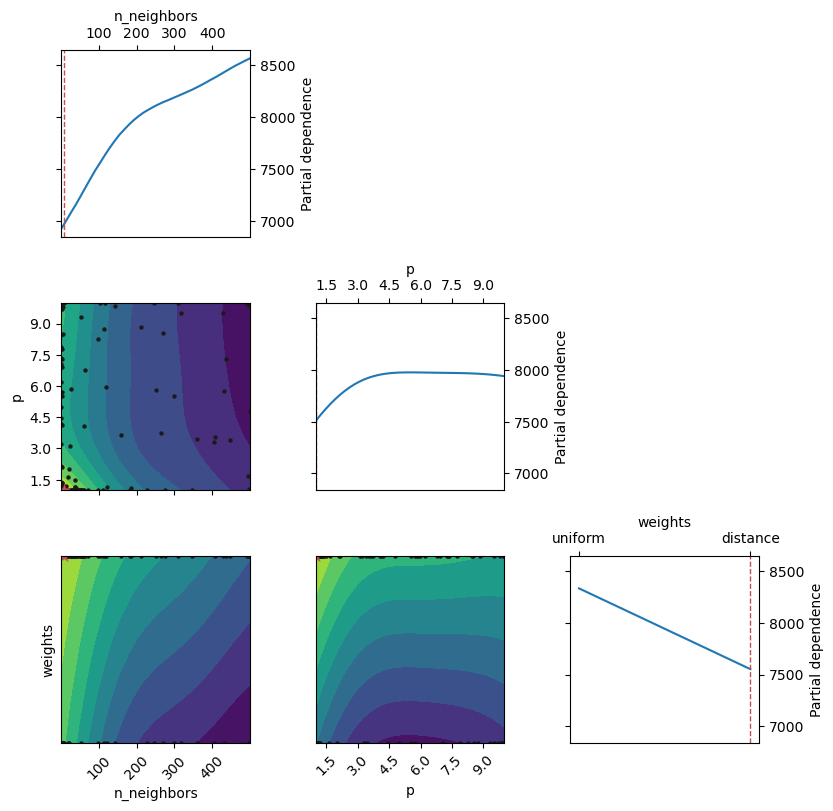
\includegraphics[keepaspectratio]{Hyperparameter tuning_files/figure-pdf/cell-23-output-1.png}}

The frequence of individual hyperparameter values considered can also be
visualized as below.

\begin{Shaded}
\begin{Highlighting}[]
\NormalTok{fig, ax }\OperatorTok{=}\NormalTok{ plt.subplots(}\DecValTok{1}\NormalTok{, }\DecValTok{3}\NormalTok{, figsize }\OperatorTok{=}\NormalTok{ (}\DecValTok{10}\NormalTok{, }\DecValTok{3}\NormalTok{))}
\NormalTok{plt.subplots\_adjust(wspace}\OperatorTok{=}\FloatTok{0.4}\NormalTok{)}
\NormalTok{plot\_histogram(gcv.optimizer\_results\_[}\DecValTok{0}\NormalTok{], }\DecValTok{0}\NormalTok{, ax }\OperatorTok{=}\NormalTok{ ax[}\DecValTok{0}\NormalTok{])}
\NormalTok{plot\_histogram(gcv.optimizer\_results\_[}\DecValTok{0}\NormalTok{], }\DecValTok{1}\NormalTok{, ax }\OperatorTok{=}\NormalTok{ ax[}\DecValTok{1}\NormalTok{])}
\NormalTok{plot\_histogram(gcv.optimizer\_results\_[}\DecValTok{0}\NormalTok{], }\DecValTok{2}\NormalTok{, ax }\OperatorTok{=}\NormalTok{ ax[}\DecValTok{2}\NormalTok{])}
\NormalTok{plt.show()}
\end{Highlighting}
\end{Shaded}

\pandocbounded{\includegraphics[keepaspectratio]{Hyperparameter tuning_files/figure-pdf/cell-24-output-1.png}}

Below is the plot showing the minimum cross-validated score computed
obtained until `n' hyperparameter values are considered for
cross-validation.

\begin{Shaded}
\begin{Highlighting}[]
\NormalTok{plot\_convergence(gcv.optimizer\_results\_)}
\NormalTok{plt.show()}
\end{Highlighting}
\end{Shaded}

\pandocbounded{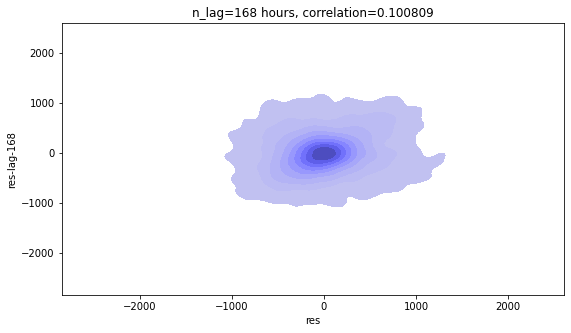
\includegraphics[keepaspectratio]{Hyperparameter tuning_files/figure-pdf/cell-25-output-1.png}}

Note that the cross-validated error is close to the optmial value in the
53rd iteration itself.

The cross-validated error at the 53rd iteration is:

\begin{Shaded}
\begin{Highlighting}[]
\NormalTok{gcv.optimizer\_results\_[}\DecValTok{0}\NormalTok{][}\StringTok{\textquotesingle{}func\_vals\textquotesingle{}}\NormalTok{][}\DecValTok{53}\NormalTok{]}
\end{Highlighting}
\end{Shaded}

\begin{verbatim}
5831.87280274334
\end{verbatim}

The hyperparameter values at the 53rd iterations are:

\begin{Shaded}
\begin{Highlighting}[]
\NormalTok{gcv.optimizer\_results\_[}\DecValTok{0}\NormalTok{][}\StringTok{\textquotesingle{}x\_iters\textquotesingle{}}\NormalTok{][}\DecValTok{53}\NormalTok{]}
\end{Highlighting}
\end{Shaded}

\begin{verbatim}
[15, 1.0, 'distance']
\end{verbatim}

Note that this is the 2nd most optimal hyperparameter value based on
\texttt{GridSearchCV()}.

Below is the plot showing the cross-validated score computed at each of
the 180 hyperparameter values considered for cross-validation. The plot
shows that the algorithm seems to explore new regions of the domain
space, instead of just exploting the promising ones. There is a balance
between exploration and exploitation for finding the optimal
hyperparameter values that minimize the objective function \emph{(i.e.,
the function that models the cross-validated score)}.

\begin{Shaded}
\begin{Highlighting}[]
\NormalTok{sns.lineplot(x }\OperatorTok{=} \BuiltInTok{range}\NormalTok{(}\DecValTok{1}\NormalTok{, }\DecValTok{181}\NormalTok{), y }\OperatorTok{=}\NormalTok{ gcv.optimizer\_results\_[}\DecValTok{0}\NormalTok{][}\StringTok{\textquotesingle{}func\_vals\textquotesingle{}}\NormalTok{])}
\NormalTok{plt.xlabel(}\StringTok{\textquotesingle{}Iteration\textquotesingle{}}\NormalTok{)}
\NormalTok{plt.ylabel(}\StringTok{\textquotesingle{}Cross{-}validated score\textquotesingle{}}\NormalTok{)}
\NormalTok{plt.show()}\OperatorTok{;}
\end{Highlighting}
\end{Shaded}

\pandocbounded{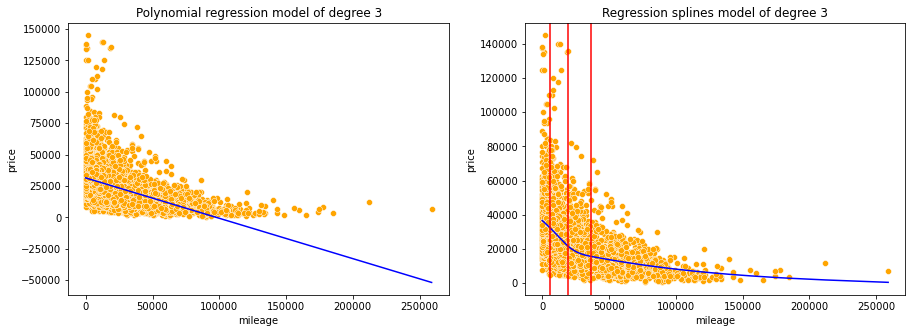
\includegraphics[keepaspectratio]{Hyperparameter tuning_files/figure-pdf/cell-28-output-1.png}}

The advantages of \texttt{BayesSearchCV()} over \texttt{GridSearchCV()}
and \texttt{RandomizedSearchCV()} are:

\begin{enumerate}
\def\labelenumi{\arabic{enumi}.}
\item
  The Bayesian Optimization approach gives the benefit that we can give
  a much larger range of possible values, since over time we identify
  and exploit the most promising regions and discard the not so
  promising ones. Plain grid-search would burn computational resources
  to explore all regions of the domain space with the same granularity,
  even the not promising ones. Since we search much more effectively in
  Bayesian search, we can search over a larger domain space.
\item
  BayesSearch CV may help us identify the optimal hyperparameter value
  in fewer iterations if the Gaussian process model estimating the
  cross-validated score is relatively accurate. However, this is not
  certain. Grid and random search are completely uninformed by past
  evaluations, and as a result, often spend a significant amount of time
  evaluating ``bad'' hyperparameters.
\item
  BayesSearch CV is more reliable in cases of a large search space,
  where random selection may miss sampling values from optimal regions
  of the search space.
\end{enumerate}

The disadvantages of \texttt{BayesSearchCV()} over
\texttt{GridSearchCV()} and \texttt{RandomizedSearchCV()} are:

\begin{enumerate}
\def\labelenumi{\arabic{enumi}.}
\item
  \texttt{BayesSearchCV()} has a cost of learning from past data, i.e.,
  updating the model that predicts the cross-validated score after every
  iteration of evaluating the cross-validated score on a new
  hyperparameter value. This cost will continue to increase as more and
  more data is collected. There is no such cost in
  \texttt{GridSearchCV()} and \texttt{RandomizedSearchCV()} as there is
  no learning. This implies that each iteration of
  \texttt{BayesSearchCV()} will take a longer time than each iteration
  of \texttt{GridSearchCV()} / \texttt{RandomizedSearchCV()}. Thus, even
  if \texttt{BayesSearchCV()} finds the optimal hyperparameter value in
  fewer iterations, it may take more time than \texttt{GridSearchCV()} /
  \texttt{RandomizedSearchCV()} for the same.
\item
  The success of \texttt{BayesSearchCV()} depends on the predictions and
  associated uncertainty estimated by the Gaussian process (GP) model
  that predicts the cross-validated score. The GP model, although works
  well in general, may not be suitable for certain datasets, or may take
  a relatively large number of iterations to learn for certain datasets.
\end{enumerate}

\subsection{Live monitoring of cross-validated
score}\label{live-monitoring-of-cross-validated-score}

Note that it will be useful monitor the cross-validated score while the
Bayesian Search CV code is running, and stop the code as soon as the
desired accuracy is reached, or the optimal cross-validated score
doesn't seem to improve. The \texttt{fit()} method of the
\texttt{BayesSeaerchCV()} object has a \texttt{callback} argument that
can be used as follows:

\begin{Shaded}
\begin{Highlighting}[]
\NormalTok{model }\OperatorTok{=}\NormalTok{ KNeighborsRegressor(metric }\OperatorTok{=} \StringTok{\textquotesingle{}minkowski\textquotesingle{}}\NormalTok{) }\CommentTok{\# No inputs defined inside the model}
\NormalTok{grid }\OperatorTok{=}\NormalTok{ \{}\StringTok{\textquotesingle{}n\_neighbors\textquotesingle{}}\NormalTok{: Integer(}\DecValTok{1}\NormalTok{, }\DecValTok{500}\NormalTok{), }\StringTok{\textquotesingle{}weights\textquotesingle{}}\NormalTok{: Categorical([}\StringTok{\textquotesingle{}uniform\textquotesingle{}}\NormalTok{, }\StringTok{\textquotesingle{}distance\textquotesingle{}}\NormalTok{]), }
       \StringTok{\textquotesingle{}p\textquotesingle{}}\NormalTok{: Real(}\DecValTok{1}\NormalTok{, }\DecValTok{10}\NormalTok{, prior }\OperatorTok{=} \StringTok{\textquotesingle{}uniform\textquotesingle{}}\NormalTok{)\} }

\NormalTok{kfold }\OperatorTok{=}\NormalTok{ KFold(n\_splits }\OperatorTok{=} \DecValTok{5}\NormalTok{, shuffle }\OperatorTok{=} \VariableTok{True}\NormalTok{, random\_state }\OperatorTok{=} \DecValTok{1}\NormalTok{)}
\NormalTok{gcv }\OperatorTok{=}\NormalTok{ BayesSearchCV(model, search\_spaces }\OperatorTok{=}\NormalTok{ grid, cv }\OperatorTok{=}\NormalTok{ kfold, n\_iter }\OperatorTok{=} \DecValTok{180}\NormalTok{, random\_state }\OperatorTok{=} \DecValTok{10}\NormalTok{,}
\NormalTok{                         scoring }\OperatorTok{=} \StringTok{\textquotesingle{}neg\_root\_mean\_squared\_error\textquotesingle{}}\NormalTok{, n\_jobs }\OperatorTok{=} \OperatorTok{{-}}\DecValTok{1}\NormalTok{)}
\end{Highlighting}
\end{Shaded}

\begin{Shaded}
\begin{Highlighting}[]
\NormalTok{paras }\OperatorTok{=} \BuiltInTok{list}\NormalTok{(gcv.search\_spaces.keys())}
\NormalTok{paras.sort()}

\KeywordTok{def}\NormalTok{ monitor(optim\_result):}
\NormalTok{    cv\_values }\OperatorTok{=}\NormalTok{ pd.Series(optim\_result[}\StringTok{\textquotesingle{}func\_vals\textquotesingle{}}\NormalTok{]).cummin()}
\NormalTok{    display.clear\_output(wait }\OperatorTok{=} \VariableTok{True}\NormalTok{)}
\NormalTok{    min\_ind }\OperatorTok{=}\NormalTok{ pd.Series(optim\_result[}\StringTok{\textquotesingle{}func\_vals\textquotesingle{}}\NormalTok{]).argmin()}
    \BuiltInTok{print}\NormalTok{(paras, }\StringTok{"="}\NormalTok{, optim\_result[}\StringTok{\textquotesingle{}x\_iters\textquotesingle{}}\NormalTok{][min\_ind], pd.Series(optim\_result[}\StringTok{\textquotesingle{}func\_vals\textquotesingle{}}\NormalTok{]).}\BuiltInTok{min}\NormalTok{())}
\NormalTok{    sns.lineplot(cv\_values)}
\NormalTok{    plt.show()}
\end{Highlighting}
\end{Shaded}

\begin{Shaded}
\begin{Highlighting}[]
\NormalTok{gcv.fit(X\_train\_scaled, y\_train, callback }\OperatorTok{=}\NormalTok{ monitor)}
\end{Highlighting}
\end{Shaded}

\begin{verbatim}
['n_neighbors', 'p', 'weights'] = [9, 1.0008321732366932, 'distance'] 5756.172382596493
\end{verbatim}

\pandocbounded{\includegraphics[keepaspectratio]{Hyperparameter tuning_files/figure-pdf/cell-31-output-2.png}}

\begin{verbatim}
BayesSearchCV(cv=KFold(n_splits=5, random_state=1, shuffle=True),
              estimator=KNeighborsRegressor(), n_iter=180, n_jobs=-1,
              random_state=10, scoring='neg_root_mean_squared_error',
              search_spaces={'n_neighbors': Integer(low=1, high=500, prior='uniform', transform='normalize'),
                             'p': Real(low=1, high=10, prior='uniform', transform='normalize'),
                             'weights': Categorical(categories=('uniform', 'distance'), prior=None)})
\end{verbatim}

\section{\texorpdfstring{\href{https://scikit-learn.org/stable/modules/generated/sklearn.model_selection.cross_validate.html}{\texttt{cross\_validate()}}}{cross\_validate()}}\label{cross_validate}

We have used \texttt{cross\_val\_score()} and
\texttt{cross\_val\_predict()} so far.

\textbf{When can we use one over the other?}

The function \texttt{cross\_validate()} is similar to
\texttt{cross\_val\_score()} except that it has the option to return
multiple cross-validated metrics, instead of a single one.

Consider the heart disease classification problem, where the response is
\texttt{target} \emph{(whether the person has a heart disease or not)}.

\begin{Shaded}
\begin{Highlighting}[]
\NormalTok{data }\OperatorTok{=}\NormalTok{ pd.read\_csv(}\StringTok{\textquotesingle{}Datasets/heart\_disease\_classification.csv\textquotesingle{}}\NormalTok{)}
\NormalTok{data.head()}
\end{Highlighting}
\end{Shaded}

\begin{longtable}[]{@{}lllllllllllllll@{}}
\toprule\noalign{}
& age & sex & cp & trestbps & chol & fbs & restecg & thalach & exang &
oldpeak & slope & ca & thal & target \\
\midrule\noalign{}
\endhead
\bottomrule\noalign{}
\endlastfoot
0 & 63 & 1 & 3 & 145 & 233 & 1 & 0 & 150 & 0 & 2.3 & 0 & 0 & 1 & 1 \\
1 & 37 & 1 & 2 & 130 & 250 & 0 & 1 & 187 & 0 & 3.5 & 0 & 0 & 2 & 1 \\
2 & 41 & 0 & 1 & 130 & 204 & 0 & 0 & 172 & 0 & 1.4 & 2 & 0 & 2 & 1 \\
3 & 56 & 1 & 1 & 120 & 236 & 0 & 1 & 178 & 0 & 0.8 & 2 & 0 & 2 & 1 \\
4 & 57 & 0 & 0 & 120 & 354 & 0 & 1 & 163 & 1 & 0.6 & 2 & 0 & 2 & 1 \\
\end{longtable}

Let us pre-process the data.

\begin{Shaded}
\begin{Highlighting}[]
\CommentTok{\# First, separate the response and the predictors}
\NormalTok{y }\OperatorTok{=}\NormalTok{ data[}\StringTok{\textquotesingle{}target\textquotesingle{}}\NormalTok{]}
\NormalTok{X }\OperatorTok{=}\NormalTok{ data.drop(}\StringTok{\textquotesingle{}target\textquotesingle{}}\NormalTok{, axis}\OperatorTok{=}\DecValTok{1}\NormalTok{)}
\end{Highlighting}
\end{Shaded}

\begin{Shaded}
\begin{Highlighting}[]
\CommentTok{\# Separate the data (X,y) into training and test}

\CommentTok{\# Inputs:}
    \CommentTok{\# data}
    \CommentTok{\# train{-}test ratio}
    \CommentTok{\# random\_state for reproducible code}
    
\NormalTok{X\_train, X\_test, y\_train, y\_test }\OperatorTok{=}\NormalTok{ train\_test\_split(X, y, test\_size}\OperatorTok{=}\FloatTok{0.2}\NormalTok{, random\_state}\OperatorTok{=}\DecValTok{20}\NormalTok{, stratify}\OperatorTok{=}\NormalTok{y) }\CommentTok{\# 80\%{-}20\% split}

\CommentTok{\# stratify=y makes sure the class 0 to class 1 ratio in the training and test sets are kept the same as the entire dataset.}
\end{Highlighting}
\end{Shaded}

\begin{Shaded}
\begin{Highlighting}[]
\NormalTok{model }\OperatorTok{=}\NormalTok{ KNeighborsClassifier() }
\NormalTok{sc }\OperatorTok{=}\NormalTok{ StandardScaler()}
\NormalTok{sc.fit(X\_train)}
\NormalTok{X\_train\_scaled }\OperatorTok{=}\NormalTok{ sc.transform(X\_train)}
\NormalTok{X\_test\_scaled }\OperatorTok{=}\NormalTok{ sc.transform(X\_test)}
\end{Highlighting}
\end{Shaded}

Suppose we want to take recall above a certain threshold with the
highest precision possible. \texttt{cross\_validate()} computes the
cross-validated score for multiple metrics - rest is the same as
\texttt{cross\_val\_score()}.

\begin{Shaded}
\begin{Highlighting}[]
\NormalTok{Ks }\OperatorTok{=}\NormalTok{ np.arange(}\DecValTok{10}\NormalTok{,}\DecValTok{200}\NormalTok{,}\DecValTok{10}\NormalTok{)}

\NormalTok{scores }\OperatorTok{=}\NormalTok{ []}

\ControlFlowTok{for}\NormalTok{ K }\KeywordTok{in}\NormalTok{ Ks:}
\NormalTok{    model }\OperatorTok{=}\NormalTok{ KNeighborsClassifier(n\_neighbors}\OperatorTok{=}\NormalTok{K) }\CommentTok{\# Keeping distance uniform}
\NormalTok{    scores.append(cross\_validate(model, X\_train\_scaled, y\_train, cv}\OperatorTok{=}\DecValTok{5}\NormalTok{, scoring }\OperatorTok{=}\NormalTok{ [}\StringTok{\textquotesingle{}accuracy\textquotesingle{}}\NormalTok{,}\StringTok{\textquotesingle{}recall\textquotesingle{}}\NormalTok{, }\StringTok{\textquotesingle{}precision\textquotesingle{}}\NormalTok{]))}
\end{Highlighting}
\end{Shaded}

\begin{Shaded}
\begin{Highlighting}[]
\NormalTok{scores}

\CommentTok{\# The output is now a list of dicts {-} easy to convert to a df}

\NormalTok{df\_scores }\OperatorTok{=}\NormalTok{ pd.DataFrame(scores) }\CommentTok{\# We need to handle test\_recall and test\_precision cols}

\NormalTok{df\_scores[}\StringTok{\textquotesingle{}CV\_recall\textquotesingle{}}\NormalTok{] }\OperatorTok{=}\NormalTok{ df\_scores[}\StringTok{\textquotesingle{}test\_recall\textquotesingle{}}\NormalTok{].}\BuiltInTok{apply}\NormalTok{(np.mean)}
\NormalTok{df\_scores[}\StringTok{\textquotesingle{}CV\_precision\textquotesingle{}}\NormalTok{] }\OperatorTok{=}\NormalTok{ df\_scores[}\StringTok{\textquotesingle{}test\_precision\textquotesingle{}}\NormalTok{].}\BuiltInTok{apply}\NormalTok{(np.mean)}
\NormalTok{df\_scores[}\StringTok{\textquotesingle{}CV\_accuracy\textquotesingle{}}\NormalTok{] }\OperatorTok{=}\NormalTok{ df\_scores[}\StringTok{\textquotesingle{}test\_accuracy\textquotesingle{}}\NormalTok{].}\BuiltInTok{apply}\NormalTok{(np.mean)}

\NormalTok{df\_scores.index }\OperatorTok{=}\NormalTok{ Ks }\CommentTok{\# We can set K values as indices for convenience}


\CommentTok{\#df\_scores}
\CommentTok{\# What happens as K increases?}
    \CommentTok{\# Recall increases (not monotonically)}
    \CommentTok{\# Precision decreases (not monotonically)}
\CommentTok{\# Why?}
    \CommentTok{\# Check the class distribution in the data {-} more obs with class 1}
    \CommentTok{\# As K gets higher, the majority class overrules (visualized in the slides)}
    \CommentTok{\# More 1s means less FNs {-} higher recall}
    \CommentTok{\# More 1s means more FPs {-} lower precision}
\CommentTok{\# Would this be the case for any dataset?}
    \CommentTok{\# NO!! Depends on what the majority class is!}
\end{Highlighting}
\end{Shaded}

Suppose we wish to have the maximum possible precision for at least 95\%
recall.

The optimal \emph{\texttt{K}} will be:

\begin{Shaded}
\begin{Highlighting}[]
\NormalTok{df\_scores.loc[df\_scores[}\StringTok{\textquotesingle{}CV\_recall\textquotesingle{}}\NormalTok{] }\OperatorTok{\textgreater{}} \FloatTok{0.95}\NormalTok{, }\StringTok{\textquotesingle{}CV\_precision\textquotesingle{}}\NormalTok{].idxmax()}
\end{Highlighting}
\end{Shaded}

\begin{verbatim}
120
\end{verbatim}

The cross-validated precision, recall and accuracy for the optimal
\emph{\texttt{K}} are:

\begin{Shaded}
\begin{Highlighting}[]
\NormalTok{df\_scores.loc[}\DecValTok{120}\NormalTok{, [}\StringTok{\textquotesingle{}CV\_recall\textquotesingle{}}\NormalTok{, }\StringTok{\textquotesingle{}CV\_precision\textquotesingle{}}\NormalTok{, }\StringTok{\textquotesingle{}CV\_accuracy\textquotesingle{}}\NormalTok{]]}
\end{Highlighting}
\end{Shaded}

\begin{verbatim}
CV_recall       0.954701
CV_precision    0.734607
CV_accuracy     0.785374
Name: 120, dtype: object
\end{verbatim}

\begin{Shaded}
\begin{Highlighting}[]
\NormalTok{sns.lineplot(x }\OperatorTok{=}\NormalTok{ df\_scores.index, y }\OperatorTok{=}\NormalTok{ df\_scores.CV\_precision, color }\OperatorTok{=} \StringTok{\textquotesingle{}blue\textquotesingle{}}\NormalTok{, label }\OperatorTok{=} \StringTok{\textquotesingle{}precision\textquotesingle{}}\NormalTok{)}
\NormalTok{sns.lineplot(x }\OperatorTok{=}\NormalTok{ df\_scores.index, y }\OperatorTok{=}\NormalTok{ df\_scores.CV\_recall, color }\OperatorTok{=} \StringTok{\textquotesingle{}red\textquotesingle{}}\NormalTok{, label }\OperatorTok{=} \StringTok{\textquotesingle{}recall\textquotesingle{}}\NormalTok{)}
\NormalTok{sns.lineplot(x }\OperatorTok{=}\NormalTok{ df\_scores.index, y }\OperatorTok{=}\NormalTok{ df\_scores.CV\_accuracy, color }\OperatorTok{=} \StringTok{\textquotesingle{}green\textquotesingle{}}\NormalTok{, label }\OperatorTok{=} \StringTok{\textquotesingle{}accuracy\textquotesingle{}}\NormalTok{)}
\NormalTok{plt.ylabel(}\StringTok{\textquotesingle{}Metric\textquotesingle{}}\NormalTok{)}
\NormalTok{plt.xlabel(}\StringTok{\textquotesingle{}K\textquotesingle{}}\NormalTok{)}
\NormalTok{plt.show()}
\end{Highlighting}
\end{Shaded}

\pandocbounded{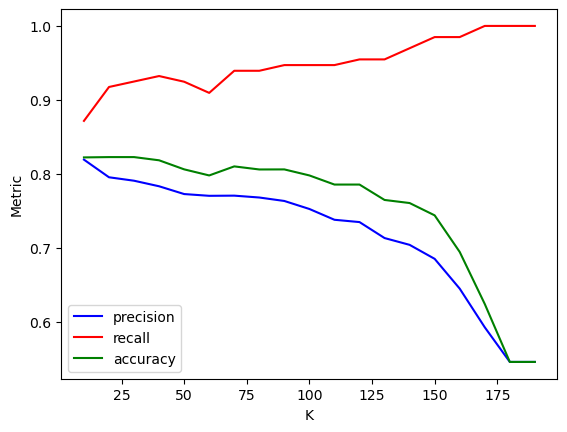
\includegraphics[keepaspectratio]{Hyperparameter tuning_files/figure-pdf/cell-40-output-1.png}}

\part{Tree based models}

\chapter{Regression trees}\label{regression-trees}

\emph{Read section 8.1.1 of the book before using these notes.}

\emph{Note that in this course, lecture notes are not sufficient, you
must read the book for better understanding. Lecture notes are just
implementing the concepts of the book on a dataset, but not explaining
the concepts elaborately.}

\begin{Shaded}
\begin{Highlighting}[]
\CommentTok{\# Importing necessary libraries}
\ImportTok{import}\NormalTok{ pandas }\ImportTok{as}\NormalTok{ pd}
\ImportTok{import}\NormalTok{ numpy }\ImportTok{as}\NormalTok{ np}
\ImportTok{import}\NormalTok{ matplotlib.pyplot }\ImportTok{as}\NormalTok{ plt}
\ImportTok{import}\NormalTok{ seaborn }\ImportTok{as}\NormalTok{ sns}
\NormalTok{sns.}\BuiltInTok{set}\NormalTok{(font\_scale}\OperatorTok{=}\FloatTok{1.35}\NormalTok{)}

\CommentTok{\# import the decision tree regressor}
\ImportTok{from}\NormalTok{ sklearn.tree }\ImportTok{import}\NormalTok{ DecisionTreeRegressor, plot\_tree, export\_graphviz}

\CommentTok{\# split the dataset into training and testing sets}
\ImportTok{from}\NormalTok{ sklearn.model\_selection }\ImportTok{import}\NormalTok{ train\_test\_split}


\ImportTok{from}\NormalTok{ sklearn.model\_selection }\ImportTok{import}\NormalTok{ cross\_val\_score, GridSearchCV, cross\_val\_predict, KFold}

\ImportTok{from}\NormalTok{ sklearn.pipeline }\ImportTok{import}\NormalTok{ Pipeline}
\ImportTok{from}\NormalTok{ sklearn.compose }\ImportTok{import}\NormalTok{ ColumnTransformer}
\ImportTok{from}\NormalTok{ sklearn.preprocessing }\ImportTok{import}\NormalTok{ OneHotEncoder, FunctionTransformer}
\ImportTok{from}\NormalTok{ sklearn.metrics }\ImportTok{import}\NormalTok{ root\_mean\_squared\_error, r2\_score, make\_scorer}
\end{Highlighting}
\end{Shaded}

We will use the same dataset as in the KNN model for regression trees.

\begin{Shaded}
\begin{Highlighting}[]
\CommentTok{\# Load the dataset}
\NormalTok{car }\OperatorTok{=}\NormalTok{ pd.read\_csv(}\StringTok{\textquotesingle{}Datasets/car.csv\textquotesingle{}}\NormalTok{)}
\NormalTok{car.head()}
\end{Highlighting}
\end{Shaded}

\begin{longtable}[]{@{}lllllllllll@{}}
\toprule\noalign{}
& brand & model & year & transmission & mileage & fuelType & tax & mpg &
engineSize & price \\
\midrule\noalign{}
\endhead
\bottomrule\noalign{}
\endlastfoot
0 & vw & Beetle & 2014 & Manual & 55457 & Diesel & 30 & 65.3266 & 1.6 &
7490 \\
1 & vauxhall & GTC & 2017 & Manual & 15630 & Petrol & 145 & 47.2049 &
1.4 & 10998 \\
2 & merc & G Class & 2012 & Automatic & 43000 & Diesel & 570 & 25.1172 &
3.0 & 44990 \\
3 & audi & RS5 & 2019 & Automatic & 10 & Petrol & 145 & 30.5593 & 2.9 &
51990 \\
4 & merc & X-CLASS & 2018 & Automatic & 14000 & Diesel & 240 & 35.7168 &
2.3 & 28990 \\
\end{longtable}

\section{Native Support for Missing
Values}\label{native-support-for-missing-values}

Starting with \textbf{scikit-learn version 1.3}, classical tree-based
models in \texttt{scikit-learn} have added \textbf{native support for
missing values}, which simplifies preprocessing and improves model
robustness:

\begin{itemize}
\tightlist
\item
  \texttt{DecisionTreeClassifier} supports missing values as of
  \textbf{version 1.3.0}\\
\item
  \texttt{RandomForestClassifier} adds support in \textbf{version 1.4.0}
\end{itemize}

This means you no longer need to impute missing values manually before
training these models.

To take advantage of this feature, first check your
\texttt{scikit-learn} version:

\begin{Shaded}
\begin{Highlighting}[]
\ImportTok{import}\NormalTok{ sklearn}
\BuiltInTok{print}\NormalTok{(sklearn.\_\_version\_\_)}
\end{Highlighting}
\end{Shaded}

\begin{verbatim}
1.6.1
\end{verbatim}

If your version is below \texttt{1.4.0}, you can upgrade by running:

\begin{Shaded}
\begin{Highlighting}[]
\CommentTok{\# pip install {-}{-}upgrade scikit{-}learn}
\end{Highlighting}
\end{Shaded}

\begin{Shaded}
\begin{Highlighting}[]
\CommentTok{\# Make a copy of the original dataset}
\NormalTok{car\_missing }\OperatorTok{=}\NormalTok{ car.copy()}

\CommentTok{\# Randomly add missing values}
\CommentTok{\# Inject missing values into 10\% of the \textquotesingle{}mileage\textquotesingle{} column}
\NormalTok{car\_missing.loc[car\_missing.sample(frac}\OperatorTok{=}\FloatTok{0.1}\NormalTok{, random\_state}\OperatorTok{=}\DecValTok{42}\NormalTok{).index, }\StringTok{\textquotesingle{}mileage\textquotesingle{}}\NormalTok{] }\OperatorTok{=}\NormalTok{ np.nan}
\CommentTok{\# Inject missing values into 10\% of the \textquotesingle{}fuelType\textquotesingle{} and \textquotesingle{}engineSize\textquotesingle{} columns}

\NormalTok{car\_missing.loc[car\_missing.sample(frac}\OperatorTok{=}\FloatTok{0.1}\NormalTok{, random\_state}\OperatorTok{=}\DecValTok{42}\NormalTok{).index, }\StringTok{\textquotesingle{}fuelType\textquotesingle{}}\NormalTok{] }\OperatorTok{=}\NormalTok{ np.nan}
\NormalTok{car\_missing.loc[car\_missing.sample(frac}\OperatorTok{=}\FloatTok{0.1}\NormalTok{, random\_state}\OperatorTok{=}\DecValTok{42}\NormalTok{).index, }\StringTok{\textquotesingle{}engineSize\textquotesingle{}}\NormalTok{] }\OperatorTok{=}\NormalTok{ np.nan}
\end{Highlighting}
\end{Shaded}

\begin{Shaded}
\begin{Highlighting}[]
\NormalTok{car\_missing.isna().}\BuiltInTok{sum}\NormalTok{()}
\end{Highlighting}
\end{Shaded}

\begin{verbatim}
brand             0
model             0
year              0
transmission      0
mileage         763
fuelType        763
tax               0
mpg               0
engineSize      763
price             0
dtype: int64
\end{verbatim}

\begin{Shaded}
\begin{Highlighting}[]
\CommentTok{\# Split the car\_missing dataset into features and target}
\NormalTok{X\_missing }\OperatorTok{=}\NormalTok{ car\_missing.drop(columns}\OperatorTok{=}\NormalTok{[}\StringTok{\textquotesingle{}price\textquotesingle{}}\NormalTok{])}
\NormalTok{y\_missing }\OperatorTok{=}\NormalTok{ car\_missing[}\StringTok{\textquotesingle{}price\textquotesingle{}}\NormalTok{]}
\end{Highlighting}
\end{Shaded}

\subsection{Build a regression tree using mileage as the solo
predictor}\label{build-a-regression-tree-using-mileage-as-the-solo-predictor}

\begin{Shaded}
\begin{Highlighting}[]
\CommentTok{\# Use only \textquotesingle{}mileage\textquotesingle{} as the feature}
\NormalTok{X\_mileage }\OperatorTok{=}\NormalTok{ X\_missing[[}\StringTok{\textquotesingle{}mileage\textquotesingle{}}\NormalTok{]]}
\NormalTok{y\_mileage }\OperatorTok{=}\NormalTok{ y\_missing}
\end{Highlighting}
\end{Shaded}

\begin{Shaded}
\begin{Highlighting}[]
\CommentTok{\# Create a DecisionTreeRegressor model}
\NormalTok{reg\_tree }\OperatorTok{=}\NormalTok{ DecisionTreeRegressor(random\_state}\OperatorTok{=}\DecValTok{42}\NormalTok{)}

\CommentTok{\# Fit the model to the data}
\NormalTok{reg\_tree.fit(X\_mileage, y\_mileage)}
\end{Highlighting}
\end{Shaded}

\begin{verbatim}
DecisionTreeRegressor(random_state=42)
\end{verbatim}

\begin{Shaded}
\begin{Highlighting}[]
\CommentTok{\# Predict the target variable using the model}
\NormalTok{y\_pred }\OperatorTok{=}\NormalTok{ reg\_tree.predict(X\_mileage)}

\CommentTok{\# Calculate the RMSE and R² score}
\NormalTok{rmse }\OperatorTok{=}\NormalTok{ np.sqrt(np.mean((y\_missing }\OperatorTok{{-}}\NormalTok{ y\_pred) }\OperatorTok{**} \DecValTok{2}\NormalTok{))}
\NormalTok{r2 }\OperatorTok{=}\NormalTok{ r2\_score(y\_missing, y\_pred)}
\BuiltInTok{print}\NormalTok{(}\SpecialStringTok{f"RMSE: }\SpecialCharTok{\{}\NormalTok{rmse}\SpecialCharTok{:.2f\}}\SpecialStringTok{"}\NormalTok{)}
\BuiltInTok{print}\NormalTok{(}\SpecialStringTok{f"R²: }\SpecialCharTok{\{}\NormalTok{r2}\SpecialCharTok{:.2f\}}\SpecialStringTok{"}\NormalTok{)}
\end{Highlighting}
\end{Shaded}

\begin{verbatim}
RMSE: 8797.85
R²: 0.71
\end{verbatim}

\section{Building regression trees}\label{building-regression-trees}

\begin{Shaded}
\begin{Highlighting}[]
\NormalTok{X }\OperatorTok{=}\NormalTok{ car.drop(columns}\OperatorTok{=}\NormalTok{[}\StringTok{\textquotesingle{}price\textquotesingle{}}\NormalTok{])}
\NormalTok{y }\OperatorTok{=}\NormalTok{ car[}\StringTok{\textquotesingle{}price\textquotesingle{}}\NormalTok{]}
\end{Highlighting}
\end{Shaded}

\begin{Shaded}
\begin{Highlighting}[]
\NormalTok{X\_train, X\_test, y\_train, y\_test }\OperatorTok{=}\NormalTok{ train\_test\_split(X, y, test\_size}\OperatorTok{=}\FloatTok{0.2}\NormalTok{, random\_state}\OperatorTok{=}\DecValTok{42}\NormalTok{)}
\end{Highlighting}
\end{Shaded}

\subsection{Using only mileage
feature}\label{using-only-mileage-feature}

\begin{Shaded}
\begin{Highlighting}[]
\CommentTok{\# Use only \textquotesingle{}mileage\textquotesingle{} as the feature}
\NormalTok{X\_train\_mileage }\OperatorTok{=}\NormalTok{ X\_train[[}\StringTok{\textquotesingle{}mileage\textquotesingle{}}\NormalTok{]]}
\NormalTok{X\_test\_mileage }\OperatorTok{=}\NormalTok{ X\_test[[}\StringTok{\textquotesingle{}mileage\textquotesingle{}}\NormalTok{]]}

\CommentTok{\# Create a DecisionTreeRegressor model}
\NormalTok{reg\_tree }\OperatorTok{=}\NormalTok{ DecisionTreeRegressor(random\_state}\OperatorTok{=}\DecValTok{42}\NormalTok{, max\_depth}\OperatorTok{=}\DecValTok{3}\NormalTok{)}

\CommentTok{\# Fit the model to the training data}
\NormalTok{reg\_tree.fit(X\_train\_mileage, y\_train)}

\CommentTok{\# Predict the target variable using the model}
\NormalTok{y\_pred }\OperatorTok{=}\NormalTok{ reg\_tree.predict(X\_test\_mileage)}

\CommentTok{\# Calculate the RMSE and R² score}
\NormalTok{rmse }\OperatorTok{=}\NormalTok{ np.sqrt(np.mean((y\_test }\OperatorTok{{-}}\NormalTok{ y\_pred) }\OperatorTok{**} \DecValTok{2}\NormalTok{))}
\NormalTok{r2 }\OperatorTok{=}\NormalTok{ r2\_score(y\_test, y\_pred)}
\BuiltInTok{print}\NormalTok{(}\SpecialStringTok{f"RMSE using only mileage predictor: }\SpecialCharTok{\{}\NormalTok{rmse}\SpecialCharTok{:.2f\}}\SpecialStringTok{"}\NormalTok{)}
\BuiltInTok{print}\NormalTok{(}\SpecialStringTok{f"R² using only mileage predictor: }\SpecialCharTok{\{}\NormalTok{r2}\SpecialCharTok{:.2f\}}\SpecialStringTok{"}\NormalTok{)}
\end{Highlighting}
\end{Shaded}

\begin{verbatim}
RMSE using only mileage predictor: 14437.80
R² using only mileage predictor: 0.29
\end{verbatim}

Let's visualize the tree structure

\begin{Shaded}
\begin{Highlighting}[]
\CommentTok{\# Plot the tree}
\NormalTok{plt.figure(figsize}\OperatorTok{=}\NormalTok{(}\DecValTok{18}\NormalTok{, }\DecValTok{6}\NormalTok{))}
\NormalTok{plot\_tree(reg\_tree, feature\_names}\OperatorTok{=}\NormalTok{[}\StringTok{\textquotesingle{}mileage\textquotesingle{}}\NormalTok{], filled}\OperatorTok{=}\VariableTok{True}\NormalTok{, rounded}\OperatorTok{=}\VariableTok{True}\NormalTok{)}
\NormalTok{plt.title(}\StringTok{"Regression Tree Using Mileage"}\NormalTok{)}
\NormalTok{plt.show()}
\end{Highlighting}
\end{Shaded}

\pandocbounded{\includegraphics[keepaspectratio]{regression_tree_sp25_files/figure-pdf/cell-15-output-1.png}}

Let's visualize how mileage is used in the decision tree below:

\begin{Shaded}
\begin{Highlighting}[]
\CommentTok{\# Create evenly spaced mileage values within the range of training data}
\NormalTok{Xtest }\OperatorTok{=}\NormalTok{ np.linspace(X\_train\_mileage[}\StringTok{\textquotesingle{}mileage\textquotesingle{}}\NormalTok{].}\BuiltInTok{min}\NormalTok{(), X\_train\_mileage[}\StringTok{\textquotesingle{}mileage\textquotesingle{}}\NormalTok{].}\BuiltInTok{max}\NormalTok{(), }\DecValTok{100}\NormalTok{).reshape(}\OperatorTok{{-}}\DecValTok{1}\NormalTok{, }\DecValTok{1}\NormalTok{)}

\CommentTok{\# Convert Xtest to a DataFrame with the correct column name}
\NormalTok{Xtest\_df }\OperatorTok{=}\NormalTok{ pd.DataFrame(Xtest, columns}\OperatorTok{=}\NormalTok{[}\StringTok{\textquotesingle{}mileage\textquotesingle{}}\NormalTok{])}

\CommentTok{\# Predict using the DataFrame instead of NumPy array}
\NormalTok{ytest\_pred }\OperatorTok{=}\NormalTok{ reg\_tree.predict(Xtest\_df)}

\NormalTok{plt.figure(figsize}\OperatorTok{=}\NormalTok{(}\DecValTok{10}\NormalTok{, }\DecValTok{6}\NormalTok{))}
\NormalTok{sns.scatterplot(x}\OperatorTok{=}\NormalTok{X\_train\_mileage[}\StringTok{\textquotesingle{}mileage\textquotesingle{}}\NormalTok{], y}\OperatorTok{=}\NormalTok{y\_train, color}\OperatorTok{=}\StringTok{\textquotesingle{}orange\textquotesingle{}}\NormalTok{, label}\OperatorTok{=}\StringTok{\textquotesingle{}Training data\textquotesingle{}}\NormalTok{)}

\CommentTok{\# Step plot to reflect piecewise constant predictions}
\NormalTok{plt.step(Xtest\_df[}\StringTok{\textquotesingle{}mileage\textquotesingle{}}\NormalTok{], ytest\_pred, color}\OperatorTok{=}\StringTok{\textquotesingle{}blue\textquotesingle{}}\NormalTok{, label}\OperatorTok{=}\StringTok{\textquotesingle{}Tree prediction\textquotesingle{}}\NormalTok{, where}\OperatorTok{=}\StringTok{\textquotesingle{}mid\textquotesingle{}}\NormalTok{)}

\NormalTok{plt.xlabel(}\StringTok{"Mileage"}\NormalTok{)}
\NormalTok{plt.ylabel(}\StringTok{"Price"}\NormalTok{)}
\NormalTok{plt.title(}\StringTok{"Decision Tree Regression: Mileage vs. Price"}\NormalTok{)}
\NormalTok{plt.legend()}
\NormalTok{plt.show()}
\end{Highlighting}
\end{Shaded}

\pandocbounded{\includegraphics[keepaspectratio]{regression_tree_sp25_files/figure-pdf/cell-16-output-1.png}}

All cars falling within the same terminal node have the same predicted
price, which is seen as flat line segments in the above model curve.

\subsection{Using mileage and brand as
predictors}\label{using-mileage-and-brand-as-predictors}

\begin{Shaded}
\begin{Highlighting}[]
\NormalTok{X\_train.head() }
\end{Highlighting}
\end{Shaded}

\begin{longtable}[]{@{}llllllllll@{}}
\toprule\noalign{}
& brand & model & year & transmission & mileage & fuelType & tax & mpg &
engineSize \\
\midrule\noalign{}
\endhead
\bottomrule\noalign{}
\endlastfoot
216 & vw & Scirocco & 2016 & Manual & 41167 & Diesel & 20 & 55.2654 &
2.0 \\
4381 & merc & CLS Class & 2018 & Semi-Auto & 12078 & Diesel & 145 &
47.7624 & 2.9 \\
6891 & hyundi & Santa Fe & 2019 & Automatic & 623 & Diesel & 145 &
43.0887 & 2.2 \\
421 & hyundi & IX35 & 2014 & Manual & 37095 & Diesel & 145 & 53.4862 &
1.7 \\
505 & ford & Edge & 2016 & Semi-Auto & 15727 & Diesel & 160 & 49.0741 &
2.0 \\
\end{longtable}

\begin{Shaded}
\begin{Highlighting}[]
\CommentTok{\# Select features and target}
\NormalTok{X\_train\_tree }\OperatorTok{=}\NormalTok{ X\_train[[}\StringTok{\textquotesingle{}mileage\textquotesingle{}}\NormalTok{, }\StringTok{\textquotesingle{}brand\textquotesingle{}}\NormalTok{]]}

\NormalTok{X\_test\_tree }\OperatorTok{=}\NormalTok{ X\_test[[}\StringTok{\textquotesingle{}mileage\textquotesingle{}}\NormalTok{, }\StringTok{\textquotesingle{}brand\textquotesingle{}}\NormalTok{]]}
\end{Highlighting}
\end{Shaded}

\begin{Shaded}
\begin{Highlighting}[]
\CommentTok{\# One{-}hot encode the categorical variable \textquotesingle{}brand\textquotesingle{}}
\NormalTok{X\_train\_tree\_encoded }\OperatorTok{=}\NormalTok{ pd.get\_dummies(X\_train\_tree, columns}\OperatorTok{=}\NormalTok{[}\StringTok{\textquotesingle{}brand\textquotesingle{}}\NormalTok{])}
\NormalTok{X\_test\_tree\_encoded }\OperatorTok{=}\NormalTok{ pd.get\_dummies(X\_test\_tree, columns}\OperatorTok{=}\NormalTok{[}\StringTok{\textquotesingle{}brand\textquotesingle{}}\NormalTok{])}
\end{Highlighting}
\end{Shaded}

\begin{Shaded}
\begin{Highlighting}[]
\NormalTok{model }\OperatorTok{=}\NormalTok{ DecisionTreeRegressor(max\_depth}\OperatorTok{=}\DecValTok{3}\NormalTok{, random\_state}\OperatorTok{=}\DecValTok{42}\NormalTok{)}
\NormalTok{model.fit(X\_train\_tree\_encoded, y\_train)}
\end{Highlighting}
\end{Shaded}

\begin{verbatim}
DecisionTreeRegressor(max_depth=3, random_state=42)
\end{verbatim}

\begin{Shaded}
\begin{Highlighting}[]
\NormalTok{plt.figure(figsize}\OperatorTok{=}\NormalTok{(}\DecValTok{12}\NormalTok{, }\DecValTok{6}\NormalTok{))}
\NormalTok{plot\_tree(model, feature\_names}\OperatorTok{=}\NormalTok{X\_train\_tree\_encoded.columns, filled}\OperatorTok{=}\VariableTok{True}\NormalTok{, rounded}\OperatorTok{=}\VariableTok{True}\NormalTok{)}
\NormalTok{plt.title(}\StringTok{"Decision Tree Using Mileage and Brand to Predict Price"}\NormalTok{)}
\NormalTok{plt.show()}
\end{Highlighting}
\end{Shaded}

\pandocbounded{\includegraphics[keepaspectratio]{regression_tree_sp25_files/figure-pdf/cell-21-output-1.png}}

\begin{Shaded}
\begin{Highlighting}[]
\CommentTok{\# Predict the target variable using the model}
\NormalTok{y\_pred\_tree }\OperatorTok{=}\NormalTok{ model.predict(X\_test\_tree\_encoded)}

\CommentTok{\# Calculate the RMSE and R² score}
\NormalTok{rmse\_tree }\OperatorTok{=}\NormalTok{ np.sqrt(np.mean((y\_test }\OperatorTok{{-}}\NormalTok{ y\_pred\_tree) }\OperatorTok{**} \DecValTok{2}\NormalTok{))}
\NormalTok{r2\_tree }\OperatorTok{=}\NormalTok{ r2\_score(y\_test, y\_pred\_tree)}
\BuiltInTok{print}\NormalTok{(}\SpecialStringTok{f"RMSE using mileage and brand predictor: }\SpecialCharTok{\{}\NormalTok{rmse\_tree}\SpecialCharTok{:.2f\}}\SpecialStringTok{"}\NormalTok{)}
\BuiltInTok{print}\NormalTok{(}\SpecialStringTok{f"R² using mileage and brand predictor: }\SpecialCharTok{\{}\NormalTok{r2\_tree}\SpecialCharTok{:.2f\}}\SpecialStringTok{"}\NormalTok{)}

\CommentTok{\# Compare the performance of the two models}
\BuiltInTok{print}\NormalTok{(}\SpecialStringTok{f"RMSE using only mileage predictor: }\SpecialCharTok{\{}\NormalTok{rmse}\SpecialCharTok{:.2f\}}\SpecialStringTok{"}\NormalTok{)}
\BuiltInTok{print}\NormalTok{(}\SpecialStringTok{f"RMSE using mileage and brand predictor: }\SpecialCharTok{\{}\NormalTok{rmse\_tree}\SpecialCharTok{:.2f\}}\SpecialStringTok{"}\NormalTok{)}
\CommentTok{\# The RMSE using mileage and brand predictor is lower than using only mileage predictor.}
\CommentTok{\# This indicates that adding the brand feature improves the model\textquotesingle{}s performance}
\end{Highlighting}
\end{Shaded}

\begin{verbatim}
RMSE using mileage and brand predictor: 12531.44
R² using mileage and brand predictor: 0.46
RMSE using only mileage predictor: 14437.80
RMSE using mileage and brand predictor: 12531.44
\end{verbatim}

\subsection{Using all predictors}\label{using-all-predictors}

Now that we've explored a single predictor (\texttt{mileage}) and added
a second predictor (\texttt{brand}), let's take it a step further and
use \textbf{all available features} to build a more robust model.

We'll construct a \textbf{pipeline} that handles necessary preprocessing
steps (e.g., categorical encoding) and fits a \textbf{Decision Tree
Regressor} in a streamlined and reproducible way.

\begin{Shaded}
\begin{Highlighting}[]
\CommentTok{\# extract the categorical columns and put them in a list}
\NormalTok{categorical\_feature }\OperatorTok{=}\NormalTok{ X.select\_dtypes(include}\OperatorTok{=}\NormalTok{[}\StringTok{\textquotesingle{}object\textquotesingle{}}\NormalTok{]).columns.tolist()}

\CommentTok{\# extract the numerical columns and put them in a list}
\NormalTok{numerical\_feature }\OperatorTok{=}\NormalTok{ X.select\_dtypes(include}\OperatorTok{=}\NormalTok{[}\StringTok{\textquotesingle{}int64\textquotesingle{}}\NormalTok{, }\StringTok{\textquotesingle{}float64\textquotesingle{}}\NormalTok{]).columns.tolist()}


\CommentTok{\# Create a ColumnTransformer to handle encoding}
\NormalTok{preprocessor }\OperatorTok{=}\NormalTok{ ColumnTransformer(}
\NormalTok{    transformers}\OperatorTok{=}\NormalTok{[}
\NormalTok{        (}\StringTok{\textquotesingle{}cat\textquotesingle{}}\NormalTok{, OneHotEncoder(handle\_unknown}\OperatorTok{=}\StringTok{\textquotesingle{}ignore\textquotesingle{}}\NormalTok{), categorical\_feature)}
\NormalTok{    ],}
\NormalTok{    remainder}\OperatorTok{=}\StringTok{\textquotesingle{}passthrough\textquotesingle{}}\NormalTok{,  }\CommentTok{\# Keep numerical feature (mileage) unchanged}
\NormalTok{    force\_int\_remainder\_cols}\OperatorTok{=}\VariableTok{False}
\NormalTok{)}

\CommentTok{\# Create the pipeline}
\NormalTok{pipeline }\OperatorTok{=}\NormalTok{ Pipeline(steps}\OperatorTok{=}\NormalTok{[}
\NormalTok{    (}\StringTok{\textquotesingle{}preprocessor\textquotesingle{}}\NormalTok{, preprocessor),}
\NormalTok{    (}\StringTok{\textquotesingle{}regressor\textquotesingle{}}\NormalTok{, DecisionTreeRegressor(max\_depth}\OperatorTok{=}\DecValTok{4}\NormalTok{, random\_state}\OperatorTok{=}\DecValTok{42}\NormalTok{))}
\NormalTok{])}

\CommentTok{\# Usage:}
\NormalTok{pipeline.fit(X\_train, y\_train)}
\NormalTok{y\_pred }\OperatorTok{=}\NormalTok{ pipeline.predict(X\_test)}

\CommentTok{\# Calculate the RMSE and R² score}
\NormalTok{rmse\_pipeline }\OperatorTok{=}\NormalTok{ np.sqrt(np.mean((y\_test }\OperatorTok{{-}}\NormalTok{ y\_pred) }\OperatorTok{**} \DecValTok{2}\NormalTok{))}
\NormalTok{r2\_pipeline }\OperatorTok{=}\NormalTok{ r2\_score(y\_test, y\_pred)}
\BuiltInTok{print}\NormalTok{(}\SpecialStringTok{f"RMSE using pipeline: }\SpecialCharTok{\{}\NormalTok{rmse\_pipeline}\SpecialCharTok{:.2f\}}\SpecialStringTok{"}\NormalTok{)}
\BuiltInTok{print}\NormalTok{(}\SpecialStringTok{f"R² using pipeline: }\SpecialCharTok{\{}\NormalTok{r2\_pipeline}\SpecialCharTok{:.2f\}}\SpecialStringTok{"}\NormalTok{)}
\end{Highlighting}
\end{Shaded}

\begin{verbatim}
RMSE using pipeline: 8186.34
R² using pipeline: 0.77
\end{verbatim}

\begin{Shaded}
\begin{Highlighting}[]
\CommentTok{\# let\textquotesingle{}s visuzalize the decision tree}

\NormalTok{plt.figure(figsize}\OperatorTok{=}\NormalTok{(}\DecValTok{12}\NormalTok{, }\DecValTok{6}\NormalTok{))}
\NormalTok{plot\_tree(pipeline.named\_steps[}\StringTok{\textquotesingle{}regressor\textquotesingle{}}\NormalTok{], feature\_names}\OperatorTok{=}\NormalTok{pipeline.named\_steps[}\StringTok{\textquotesingle{}preprocessor\textquotesingle{}}\NormalTok{].get\_feature\_names\_out(), filled}\OperatorTok{=}\VariableTok{True}\NormalTok{, rounded}\OperatorTok{=}\VariableTok{True}\NormalTok{)}
\NormalTok{plt.title(}\StringTok{"Decision Tree Using Pipeline"}\NormalTok{)}
\NormalTok{plt.show()}

\end{Highlighting}
\end{Shaded}

\pandocbounded{\includegraphics[keepaspectratio]{regression_tree_sp25_files/figure-pdf/cell-24-output-1.png}}

\section{Key Hyperparameters in Decision
Tree}\label{key-hyperparameters-in-decision-tree}

In regression trees, \textbf{model complexity} is controlled by
hyperparameters, tuning them is crucial for balancing
\textbf{underfitting} and \textbf{overfitting}.

\subsection{Underfitting}\label{underfitting}

\begin{itemize}
\tightlist
\item
  The model is \textbf{too simple} to capture patterns in the data.
\item
  High bias, low variance.
\item
  Often caused by:

  \begin{itemize}
  \tightlist
  \item
    Shallow trees (\texttt{max\_depth} is too small)
  \item
    Too strict constraints (\texttt{min\_samples\_split} or
    \texttt{min\_samples\_leaf} is too high)
  \end{itemize}
\end{itemize}

\subsection{Overfitting}\label{overfitting}

\begin{itemize}
\tightlist
\item
  The model is \textbf{too complex} and learns noise from the training
  data.
\item
  Low bias, high variance.
\item
  Often caused by:

  \begin{itemize}
  \tightlist
  \item
    Deep trees with many splits
  \item
    Very small \texttt{min\_samples\_leaf} or
    \texttt{min\_samples\_split}
  \end{itemize}
\end{itemize}

Below are the most commonly used hyperparameters:

\subsection{\texorpdfstring{\texttt{max\_depth}}{max\_depth}}\label{max_depth}

\begin{itemize}
\tightlist
\item
  Controls the \textbf{maximum depth} of the tree.
\item
  If \texttt{None}, the tree will expand until all leaves are pure or
  contain fewer than \texttt{min\_samples\_split} samples.
\item
  Controls overfitting (deep trees → overfit, shallow trees → underfit)
\item
  Typical values: 3 to 20 (start with lower values).
\end{itemize}

\subsection{\texorpdfstring{\texttt{min\_samples\_split}}{min\_samples\_split}}\label{min_samples_split}

\begin{itemize}
\tightlist
\item
  The \textbf{minimum number of samples} required to split an internal
  node.
\item
  higher values → simpler trees (reducing overfitting)
\end{itemize}

\subsection{\texorpdfstring{\texttt{min\_samples\_leaf}}{min\_samples\_leaf}}\label{min_samples_leaf}

\begin{itemize}
\tightlist
\item
  The minimum number of samples required to be at a leaf node.
\item
  Setting this to a higher number can smooth the model by reducing
  variance.
\end{itemize}

\subsection{\texorpdfstring{\texttt{max\_features}}{max\_features}}\label{max_features}

\begin{itemize}
\item
  Number of features to consider when looking for the best split.
\item
  Can be set to:

  \begin{itemize}
  \tightlist
  \item
    \texttt{"auto"} or \texttt{None}: use all features
  \item
    \texttt{"sqrt"}: use the square root of the number of features
  \item
    \texttt{"log2"}: use log base 2
  \end{itemize}
\end{itemize}

\begin{Shaded}
\begin{Highlighting}[]
\CommentTok{\# Define your parameter grid with pipeline step prefix}
\NormalTok{param\_grid }\OperatorTok{=}\NormalTok{ \{}
    \StringTok{\textquotesingle{}regressor\_\_max\_depth\textquotesingle{}}\NormalTok{: [}\DecValTok{3}\NormalTok{, }\DecValTok{5}\NormalTok{, }\DecValTok{7}\NormalTok{, }\DecValTok{10}\NormalTok{, }\VariableTok{None}\NormalTok{],}
    \StringTok{\textquotesingle{}regressor\_\_min\_samples\_split\textquotesingle{}}\NormalTok{: [}\DecValTok{2}\NormalTok{, }\DecValTok{5}\NormalTok{, }\DecValTok{10}\NormalTok{],}
    \StringTok{\textquotesingle{}regressor\_\_min\_samples\_leaf\textquotesingle{}}\NormalTok{: [}\DecValTok{1}\NormalTok{, }\DecValTok{2}\NormalTok{, }\DecValTok{4}\NormalTok{],}
    \StringTok{\textquotesingle{}regressor\_\_max\_features\textquotesingle{}}\NormalTok{: [}\StringTok{\textquotesingle{}sqrt\textquotesingle{}}\NormalTok{, }\VariableTok{None}\NormalTok{]}
\NormalTok{\}}

\CommentTok{\# Create custom scorer for RMSE}
\NormalTok{rmse\_scorer }\OperatorTok{=}\NormalTok{ make\_scorer(}\KeywordTok{lambda}\NormalTok{ y\_true, y\_pred: root\_mean\_squared\_error(y\_true, y\_pred),}
\NormalTok{                          greater\_is\_better}\OperatorTok{=}\VariableTok{False}\NormalTok{)}
\CommentTok{\# Create GridSearchCV object}
\NormalTok{grid\_search }\OperatorTok{=}\NormalTok{ GridSearchCV(}
\NormalTok{    estimator}\OperatorTok{=}\NormalTok{pipeline,}
\NormalTok{    param\_grid}\OperatorTok{=}\NormalTok{param\_grid,}
\NormalTok{    scoring}\OperatorTok{=}\NormalTok{\{}
        \StringTok{\textquotesingle{}RMSE\textquotesingle{}}\NormalTok{: rmse\_scorer,}
        \StringTok{\textquotesingle{}R2\textquotesingle{}}\NormalTok{: }\StringTok{\textquotesingle{}r2\textquotesingle{}}
\NormalTok{    \},}
\NormalTok{    refit}\OperatorTok{=}\StringTok{\textquotesingle{}R2\textquotesingle{}}\NormalTok{,}
\NormalTok{    cv}\OperatorTok{=}\DecValTok{5}\NormalTok{,}
\NormalTok{    n\_jobs}\OperatorTok{={-}}\DecValTok{1}\NormalTok{,}
\NormalTok{    verbose}\OperatorTok{=}\DecValTok{1}
\NormalTok{)}

\CommentTok{\# Fit the grid search to training data}
\NormalTok{grid\_search.fit(X\_train, y\_train)}
\end{Highlighting}
\end{Shaded}

\begin{verbatim}
Fitting 5 folds for each of 270 candidates, totalling 1350 fits
\end{verbatim}

\begin{verbatim}
GridSearchCV(cv=5,
             estimator=Pipeline(steps=[('preprocessor',
                                        ColumnTransformer(force_int_remainder_cols=False,
                                                          remainder='passthrough',
                                                          transformers=[('cat',
                                                                         OneHotEncoder(handle_unknown='ignore'),
                                                                         ['brand',
                                                                          'model',
                                                                          'transmission',
                                                                          'fuelType'])])),
                                       ('regressor',
                                        DecisionTreeRegressor(max_depth=4,
                                                              random_state=42))]),
             n_jobs=-1,
             param_grid={'regressor__ccp_alpha': [0.001, 0.01, 0.1],
                         'regressor__max_depth': [3, 5, 7, 10, None],
                         'regressor__max_features': ['sqrt', None],
                         'regressor__min_samples_leaf': [1, 2, 4],
                         'regressor__min_samples_split': [2, 5, 10]},
             refit='R2',
             scoring={'R2': 'r2',
                      'RMSE': make_scorer(<lambda>, greater_is_better=False, response_method='predict')},
             verbose=1)
\end{verbatim}

The \texttt{GridSearchCV} setup evaluates both \textbf{RMSE} and
\textbf{R²} during cross-validation.

\begin{itemize}
\tightlist
\item
  \textbf{R²} is used to \textbf{select the best model} and is also used
  to \textbf{refit} the model on the entire training set.
\item
  \textbf{RMSE} is computed during the process for evaluation purposes,
  but it is \textbf{not used to determine} the best model.
\end{itemize}

This allows for more comprehensive model assessment while still
optimizing based on a single selected metric.

\begin{Shaded}
\begin{Highlighting}[]
\CommentTok{\# Get best estimator and predictions}
\NormalTok{best\_model }\OperatorTok{=}\NormalTok{ grid\_search.best\_estimator\_}
\NormalTok{y\_pred\_tuned }\OperatorTok{=}\NormalTok{ best\_model.predict(X\_test)}

\CommentTok{\# Calculate metrics for tuned model}
\NormalTok{rmse\_tuned }\OperatorTok{=}\NormalTok{ root\_mean\_squared\_error(y\_test, y\_pred\_tuned)}
\NormalTok{r2\_tuned }\OperatorTok{=}\NormalTok{ r2\_score(y\_test, y\_pred\_tuned)}
\end{Highlighting}
\end{Shaded}

\begin{Shaded}
\begin{Highlighting}[]
\BuiltInTok{print}\NormalTok{(}\StringTok{"}\CharTok{\textbackslash{}n}\StringTok{=== Best Parameters ==="}\NormalTok{)}
\BuiltInTok{print}\NormalTok{(grid\_search.best\_params\_)}
\BuiltInTok{print}\NormalTok{(}\StringTok{"}\CharTok{\textbackslash{}n}\StringTok{=== Tuned Model Performance ==="}\NormalTok{)}
\BuiltInTok{print}\NormalTok{(}\SpecialStringTok{f"RMSE (Tuned): }\SpecialCharTok{\{}\NormalTok{rmse\_tuned}\SpecialCharTok{:.2f\}}\SpecialStringTok{"}\NormalTok{)}
\BuiltInTok{print}\NormalTok{(}\SpecialStringTok{f"R² (Tuned): }\SpecialCharTok{\{}\NormalTok{r2\_tuned}\SpecialCharTok{:.2f\}}\SpecialStringTok{"}\NormalTok{)}
\BuiltInTok{print}\NormalTok{(}\SpecialStringTok{f"Improvement in R²: }\SpecialCharTok{\{}\NormalTok{(r2\_tuned }\OperatorTok{{-}}\NormalTok{ r2\_pipeline)}\SpecialCharTok{:.2\%\}}\SpecialStringTok{"}\NormalTok{)}
\end{Highlighting}
\end{Shaded}

\begin{verbatim}

=== Best Parameters ===
{'regressor__ccp_alpha': 0.001, 'regressor__max_depth': None, 'regressor__max_features': None, 'regressor__min_samples_leaf': 1, 'regressor__min_samples_split': 5}

=== Tuned Model Performance ===
RMSE (Tuned): 4726.17
R² (Tuned): 0.92
Improvement in R²: 15.23%
\end{verbatim}

\begin{Shaded}
\begin{Highlighting}[]
\BuiltInTok{print}\NormalTok{(}\StringTok{"}\CharTok{\textbackslash{}n}\StringTok{=== Best Parameters ==="}\NormalTok{)}
\BuiltInTok{print}\NormalTok{(grid\_search.best\_params\_)}
\BuiltInTok{print}\NormalTok{(}\StringTok{"}\CharTok{\textbackslash{}n}\StringTok{=== Tuned Model Performance ==="}\NormalTok{)}
\BuiltInTok{print}\NormalTok{(}\SpecialStringTok{f"RMSE (Tuned): }\SpecialCharTok{\{}\NormalTok{rmse\_tuned}\SpecialCharTok{:.2f\}}\SpecialStringTok{"}\NormalTok{)}
\BuiltInTok{print}\NormalTok{(}\SpecialStringTok{f"R² (Tuned): }\SpecialCharTok{\{}\NormalTok{r2\_tuned}\SpecialCharTok{:.2f\}}\SpecialStringTok{"}\NormalTok{)}
\BuiltInTok{print}\NormalTok{(}\SpecialStringTok{f"Improvement in R²: }\SpecialCharTok{\{}\NormalTok{(r2\_tuned }\OperatorTok{{-}}\NormalTok{ r2\_pipeline)}\SpecialCharTok{:.2\%\}}\SpecialStringTok{"}\NormalTok{)}
\end{Highlighting}
\end{Shaded}

\begin{verbatim}

=== Best Parameters ===
{'regressor__ccp_alpha': 0.001, 'regressor__max_depth': None, 'regressor__max_features': None, 'regressor__min_samples_leaf': 1, 'regressor__min_samples_split': 5}

=== Tuned Model Performance ===
RMSE (Tuned): 4726.17
R² (Tuned): 0.92
Improvement in R²: 15.23%
\end{verbatim}

\texttt{GridSearchCV} improves the r squared from 0.77 to 0.92,
increased by 15.23\%, Let us visualize the mean squared error based on
the hyperparameter values. We'll use the cross validation results stored
in the cv\_results\_ attribute of the GridSearchCV fit() object.

\begin{Shaded}
\begin{Highlighting}[]
\CommentTok{\#Detailed results of k{-}fold cross validation}
\NormalTok{cv\_results }\OperatorTok{=}\NormalTok{ pd.DataFrame(grid\_search.cv\_results\_)}
\NormalTok{cv\_results.head()}
\end{Highlighting}
\end{Shaded}

\begin{longtable}[]{@{}llllllllllllllllllllll@{}}
\toprule\noalign{}
& mean\_fit\_time & std\_fit\_time & mean\_score\_time &
std\_score\_time & param\_regressor\_\_ccp\_alpha &
param\_regressor\_\_max\_depth & param\_regressor\_\_max\_features &
param\_regressor\_\_min\_samples\_leaf &
param\_regressor\_\_min\_samples\_split & params & ... & std\_test\_RMSE
& rank\_test\_RMSE & split0\_test\_R2 & split1\_test\_R2 &
split2\_test\_R2 & split3\_test\_R2 & split4\_test\_R2 & mean\_test\_R2
& std\_test\_R2 & rank\_test\_R2 \\
\midrule\noalign{}
\endhead
\bottomrule\noalign{}
\endlastfoot
0 & 0.075184 & 0.013049 & 0.009999 & 0.001052 & 0.001 & 3 & sqrt & 1 & 2
& \{\textquotesingle regressor\_\_ccp\_alpha\textquotesingle: 0.001,
\textquotesingle regressor\_\_ma... & ... & 607.458245 & 250 & 0.42527 &
0.37778 & 0.538252 & 0.37182 & 0.364829 & 0.415590 & 0.064903 & 250 \\
1 & 0.078505 & 0.014115 & 0.010804 & 0.001051 & 0.001 & 3 & sqrt & 1 & 5
& \{\textquotesingle regressor\_\_ccp\_alpha\textquotesingle: 0.001,
\textquotesingle regressor\_\_ma... & ... & 607.458245 & 250 & 0.42527 &
0.37778 & 0.538252 & 0.37182 & 0.364829 & 0.415590 & 0.064903 & 250 \\
2 & 0.077370 & 0.011081 & 0.010873 & 0.000946 & 0.001 & 3 & sqrt & 1 &
10 & \{\textquotesingle regressor\_\_ccp\_alpha\textquotesingle: 0.001,
\textquotesingle regressor\_\_ma... & ... & 606.926403 & 244 & 0.42527 &
0.37778 & 0.538252 & 0.37182 & 0.365155 & 0.415655 & 0.064852 & 244 \\
3 & 0.036274 & 0.036182 & 0.010617 & 0.000345 & 0.001 & 3 & sqrt & 2 & 2
& \{\textquotesingle regressor\_\_ccp\_alpha\textquotesingle: 0.001,
\textquotesingle regressor\_\_ma... & ... & 607.458245 & 250 & 0.42527 &
0.37778 & 0.538252 & 0.37182 & 0.364829 & 0.415590 & 0.064903 & 250 \\
4 & 0.018702 & 0.003564 & 0.012120 & 0.004090 & 0.001 & 3 & sqrt & 2 & 5
& \{\textquotesingle regressor\_\_ccp\_alpha\textquotesingle: 0.001,
\textquotesingle regressor\_\_ma... & ... & 607.458245 & 250 & 0.42527 &
0.37778 & 0.538252 & 0.37182 & 0.364829 & 0.415590 & 0.064903 & 250 \\
\end{longtable}

\begin{Shaded}
\begin{Highlighting}[]
\CommentTok{\# Plotting the RMSE for different max\_depth values}
\NormalTok{plt.figure(figsize}\OperatorTok{=}\NormalTok{(}\DecValTok{12}\NormalTok{, }\DecValTok{6}\NormalTok{))}
\NormalTok{sns.lineplot(data}\OperatorTok{=}\NormalTok{cv\_results, x}\OperatorTok{=}\StringTok{\textquotesingle{}param\_regressor\_\_max\_depth\textquotesingle{}}\NormalTok{, y}\OperatorTok{=}\NormalTok{np.}\BuiltInTok{abs}\NormalTok{(cv\_results[}\StringTok{\textquotesingle{}mean\_test\_RMSE\textquotesingle{}}\NormalTok{]), marker}\OperatorTok{=}\StringTok{\textquotesingle{}o\textquotesingle{}}\NormalTok{)}
\NormalTok{plt.xlabel(}\StringTok{\textquotesingle{}Max Depth\textquotesingle{}}\NormalTok{)}
\NormalTok{plt.ylabel(}\StringTok{\textquotesingle{}Mean Test RMSE\textquotesingle{}}\NormalTok{)}
\NormalTok{plt.title(}\StringTok{\textquotesingle{}RMSE vs Max Depth\textquotesingle{}}\NormalTok{)}\OperatorTok{;}
\end{Highlighting}
\end{Shaded}

\pandocbounded{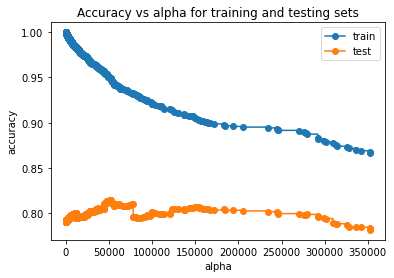
\includegraphics[keepaspectratio]{regression_tree_sp25_files/figure-pdf/cell-30-output-1.png}}

\subsection{Output feature importance}\label{output-feature-importance}

\begin{Shaded}
\begin{Highlighting}[]
\CommentTok{\# Get feature importances and names}
\NormalTok{feature\_importances }\OperatorTok{=}\NormalTok{ best\_model.named\_steps[}\StringTok{\textquotesingle{}regressor\textquotesingle{}}\NormalTok{].feature\_importances\_}
\NormalTok{feature\_names }\OperatorTok{=}\NormalTok{ best\_model.named\_steps[}\StringTok{\textquotesingle{}preprocessor\textquotesingle{}}\NormalTok{].get\_feature\_names\_out()}

\CommentTok{\# Create DataFrame and select top 10}
\NormalTok{feature\_importance\_df }\OperatorTok{=}\NormalTok{ (}
\NormalTok{    pd.DataFrame(\{}\StringTok{\textquotesingle{}Feature\textquotesingle{}}\NormalTok{: feature\_names, }\StringTok{\textquotesingle{}Importance\textquotesingle{}}\NormalTok{: feature\_importances\})}
\NormalTok{    .sort\_values(by}\OperatorTok{=}\StringTok{\textquotesingle{}Importance\textquotesingle{}}\NormalTok{, ascending}\OperatorTok{=}\VariableTok{False}\NormalTok{)}
\NormalTok{    .head(}\DecValTok{10}\NormalTok{)  }\CommentTok{\# Keep only top 10 features}
\NormalTok{)}

\CommentTok{\# Print top 10 features}
\BuiltInTok{print}\NormalTok{(}\StringTok{"=== Top 10 Feature Importances ==="}\NormalTok{)}
\BuiltInTok{print}\NormalTok{(feature\_importance\_df)}

\CommentTok{\# Plot top 10 features}
\NormalTok{plt.figure(figsize}\OperatorTok{=}\NormalTok{(}\DecValTok{12}\NormalTok{, }\DecValTok{6}\NormalTok{))}
\NormalTok{sns.barplot(data}\OperatorTok{=}\NormalTok{feature\_importance\_df, x}\OperatorTok{=}\StringTok{\textquotesingle{}Importance\textquotesingle{}}\NormalTok{, y}\OperatorTok{=}\StringTok{\textquotesingle{}Feature\textquotesingle{}}\NormalTok{)}
\NormalTok{plt.title(}\StringTok{\textquotesingle{}Top 10 Feature Importances from Decision Tree\textquotesingle{}}\NormalTok{)}
\NormalTok{plt.xlabel(}\StringTok{\textquotesingle{}Importance\textquotesingle{}}\NormalTok{)}
\NormalTok{plt.ylabel(}\StringTok{\textquotesingle{}Feature\textquotesingle{}}\NormalTok{)}
\NormalTok{plt.tight\_layout()}
\NormalTok{plt.show()}
\end{Highlighting}
\end{Shaded}

\begin{verbatim}
=== Top 10 Feature Importances ===
                   Feature  Importance
112  remainder__engineSize    0.437921
109     remainder__mileage    0.173215
108        remainder__year    0.149303
111         remainder__mpg    0.086922
98          cat__model_ i8    0.017971
2          cat__brand_ford    0.013837
92          cat__model_ X7    0.013477
110         remainder__tax    0.011502
60     cat__model_ Mustang    0.009517
86     cat__model_ V Class    0.008147
\end{verbatim}

\pandocbounded{\includegraphics[keepaspectratio]{regression_tree_sp25_files/figure-pdf/cell-31-output-2.png}}

\section{\texorpdfstring{Cost-Complexity Pruning
(\texttt{ccp\_alpha})}{Cost-Complexity Pruning (ccp\_alpha)}}\label{cost-complexity-pruning-ccp_alpha}

Cost-complexity pruning is a post-pruning technique used to reduce the
size of a decision tree by removing sections that provide little to no
improvement in prediction accuracy. It helps prevent
\textbf{overfitting} and improves \textbf{model generalization}.

\subsection{Key Idea}\label{key-idea}

Each subtree in a decision tree has an associated
\textbf{cost-complexity score}:

\$ R\_\alpha(T) = R(T) + \alpha \cdot \textbar T\textbar{} \$

\begin{itemize}
\tightlist
\item
  \$ R(T) \$: Total training error of the tree ( T )
\item
  \$ \textbar T\textbar{} \$: Number of leaf nodes in the tree
\item
  \(alpha\) (\textbf{ccp\_alpha}): Complexity parameter that penalizes
  tree size
\end{itemize}

As \(alpha\) increases, the tree is \textbf{pruned more aggressively}.

\subsection{\texorpdfstring{Parameter: \texttt{ccp\_alpha} in
scikit-learn}{Parameter: ccp\_alpha in scikit-learn}}\label{parameter-ccp_alpha-in-scikit-learn}

\begin{itemize}
\tightlist
\item
  Available in \texttt{DecisionTreeRegressor} and
  \texttt{DecisionTreeClassifier}
\item
  Default: \texttt{ccp\_alpha\ =\ 0.0} (no pruning)
\item
  Increasing \texttt{ccp\_alpha} encourages simpler trees by penalizing
  extra leaf nodes
\end{itemize}

\begin{Shaded}
\begin{Highlighting}[]
\ImportTok{from}\NormalTok{ sklearn.model\_selection }\ImportTok{import}\NormalTok{ GridSearchCV}
\ImportTok{from}\NormalTok{ sklearn.metrics }\ImportTok{import}\NormalTok{ make\_scorer, mean\_squared\_error}
\ImportTok{import}\NormalTok{ numpy }\ImportTok{as}\NormalTok{ np}

\CommentTok{\# Define your parameter grid with pipeline step prefix}
\NormalTok{param\_grid }\OperatorTok{=}\NormalTok{ \{}
    \StringTok{\textquotesingle{}regressor\_\_ccp\_alpha\textquotesingle{}}\NormalTok{: [}\FloatTok{0.0}\NormalTok{, }\FloatTok{0.001}\NormalTok{, }\FloatTok{0.01}\NormalTok{, }\FloatTok{0.1}\NormalTok{]}
\NormalTok{\}}

\CommentTok{\# Create custom scorer for RMSE}
\NormalTok{rmse\_scorer }\OperatorTok{=}\NormalTok{ make\_scorer(}\KeywordTok{lambda}\NormalTok{ y\_true, y\_pred: np.sqrt(mean\_squared\_error(y\_true, y\_pred)),}
\NormalTok{                          greater\_is\_better}\OperatorTok{=}\VariableTok{False}\NormalTok{)}

\CommentTok{\# Create GridSearchCV object}
\NormalTok{grid\_search\_ccp }\OperatorTok{=}\NormalTok{ GridSearchCV(}
\NormalTok{    estimator}\OperatorTok{=}\NormalTok{pipeline,}
\NormalTok{    param\_grid}\OperatorTok{=}\NormalTok{param\_grid,}
\NormalTok{    scoring}\OperatorTok{=}\NormalTok{\{}
        \StringTok{\textquotesingle{}RMSE\textquotesingle{}}\NormalTok{: rmse\_scorer,}
        \StringTok{\textquotesingle{}R2\textquotesingle{}}\NormalTok{: }\StringTok{\textquotesingle{}r2\textquotesingle{}}
\NormalTok{    \},}
\NormalTok{    refit}\OperatorTok{=}\StringTok{\textquotesingle{}R2\textquotesingle{}}\NormalTok{,}
\NormalTok{    cv}\OperatorTok{=}\DecValTok{5}\NormalTok{,}
\NormalTok{    n\_jobs}\OperatorTok{={-}}\DecValTok{1}\NormalTok{,}
\NormalTok{    verbose}\OperatorTok{=}\DecValTok{1}
\NormalTok{)}

\CommentTok{\# Fit the grid search to training data}
\NormalTok{grid\_search\_ccp.fit(X\_train, y\_train)}
\end{Highlighting}
\end{Shaded}

\begin{verbatim}
Fitting 5 folds for each of 4 candidates, totalling 20 fits
\end{verbatim}

\begin{verbatim}
GridSearchCV(cv=5,
             estimator=Pipeline(steps=[('preprocessor',
                                        ColumnTransformer(force_int_remainder_cols=False,
                                                          remainder='passthrough',
                                                          transformers=[('cat',
                                                                         OneHotEncoder(handle_unknown='ignore'),
                                                                         ['brand',
                                                                          'model',
                                                                          'transmission',
                                                                          'fuelType'])])),
                                       ('regressor',
                                        DecisionTreeRegressor(max_depth=4,
                                                              random_state=42))]),
             n_jobs=-1,
             param_grid={'regressor__ccp_alpha': [0.0, 0.001, 0.01, 0.1]},
             refit='R2',
             scoring={'R2': 'r2',
                      'RMSE': make_scorer(<lambda>, greater_is_better=False, response_method='predict')},
             verbose=1)
\end{verbatim}

\begin{Shaded}
\begin{Highlighting}[]
\NormalTok{encoder }\OperatorTok{=}\NormalTok{ OneHotEncoder(handle\_unknown}\OperatorTok{=}\StringTok{\textquotesingle{}ignore\textquotesingle{}}\NormalTok{, sparse\_output}\OperatorTok{=}\VariableTok{False}\NormalTok{)}

\NormalTok{X\_train\_encoded }\OperatorTok{=}\NormalTok{ encoder.fit\_transform(X\_train[categorical\_feature])}
\NormalTok{X\_test\_encoded }\OperatorTok{=}\NormalTok{ encoder.transform(X\_test[categorical\_feature])}

\CommentTok{\# Convert the encoded features back to DataFrame}
\NormalTok{X\_train\_encoded\_df }\OperatorTok{=}\NormalTok{ pd.DataFrame(X\_train\_encoded, columns}\OperatorTok{=}\NormalTok{encoder.get\_feature\_names\_out(categorical\_feature))}
\NormalTok{X\_test\_encoded\_df }\OperatorTok{=}\NormalTok{ pd.DataFrame(X\_test\_encoded, columns}\OperatorTok{=}\NormalTok{encoder.get\_feature\_names\_out(categorical\_feature))}

\CommentTok{\# Concatenate the encoded features with the original numerical features}
\NormalTok{X\_train\_final }\OperatorTok{=}\NormalTok{ pd.concat([X\_train\_encoded\_df, X\_train[numerical\_feature].reset\_index(drop}\OperatorTok{=}\VariableTok{True}\NormalTok{)], axis}\OperatorTok{=}\DecValTok{1}\NormalTok{)}
\NormalTok{X\_test\_final }\OperatorTok{=}\NormalTok{ pd.concat([X\_test\_encoded\_df, X\_test[numerical\_feature].reset\_index(drop}\OperatorTok{=}\VariableTok{True}\NormalTok{)], axis}\OperatorTok{=}\DecValTok{1}\NormalTok{)}

\CommentTok{\# Check the final shape of the training and testing sets}
\BuiltInTok{print}\NormalTok{(}\StringTok{"Training set shape:"}\NormalTok{, X\_train\_final.shape)}
\BuiltInTok{print}\NormalTok{(}\StringTok{"Testing set shape:"}\NormalTok{, X\_test\_final.shape)}
\CommentTok{\# Check the first few rows of the final training set}
\NormalTok{X\_train\_final.head()}
\CommentTok{\# Check the first few rows of the final testing set}
\end{Highlighting}
\end{Shaded}

\begin{verbatim}
Training set shape: (6105, 113)
Testing set shape: (1527, 113)
\end{verbatim}

\begin{longtable}[]{@{}llllllllllllllllllllll@{}}
\toprule\noalign{}
& brand\_audi & brand\_bmw & brand\_ford & brand\_hyundi & brand\_merc &
brand\_skoda & brand\_toyota & brand\_vauxhall & brand\_vw & model\_ 6
Series & ... & fuelType\_Diesel & fuelType\_Electric & fuelType\_Hybrid
& fuelType\_Other & fuelType\_Petrol & year & mileage & tax & mpg &
engineSize \\
\midrule\noalign{}
\endhead
\bottomrule\noalign{}
\endlastfoot
0 & 0.0 & 0.0 & 0.0 & 0.0 & 0.0 & 0.0 & 0.0 & 0.0 & 1.0 & 0.0 & ... &
1.0 & 0.0 & 0.0 & 0.0 & 0.0 & 2016 & 41167 & 20 & 55.2654 & 2.0 \\
1 & 0.0 & 0.0 & 0.0 & 0.0 & 1.0 & 0.0 & 0.0 & 0.0 & 0.0 & 0.0 & ... &
1.0 & 0.0 & 0.0 & 0.0 & 0.0 & 2018 & 12078 & 145 & 47.7624 & 2.9 \\
2 & 0.0 & 0.0 & 0.0 & 1.0 & 0.0 & 0.0 & 0.0 & 0.0 & 0.0 & 0.0 & ... &
1.0 & 0.0 & 0.0 & 0.0 & 0.0 & 2019 & 623 & 145 & 43.0887 & 2.2 \\
3 & 0.0 & 0.0 & 0.0 & 1.0 & 0.0 & 0.0 & 0.0 & 0.0 & 0.0 & 0.0 & ... &
1.0 & 0.0 & 0.0 & 0.0 & 0.0 & 2014 & 37095 & 145 & 53.4862 & 1.7 \\
4 & 0.0 & 0.0 & 1.0 & 0.0 & 0.0 & 0.0 & 0.0 & 0.0 & 0.0 & 0.0 & ... &
1.0 & 0.0 & 0.0 & 0.0 & 0.0 & 2016 & 15727 & 160 & 49.0741 & 2.0 \\
\end{longtable}

\begin{Shaded}
\begin{Highlighting}[]
\NormalTok{model }\OperatorTok{=}\NormalTok{ DecisionTreeRegressor(random\_state }\OperatorTok{=} \DecValTok{1}\NormalTok{)}\CommentTok{\#model without any restrictions}
\NormalTok{path}\OperatorTok{=}\NormalTok{ model.cost\_complexity\_pruning\_path(X\_train\_final,y\_train)}\CommentTok{\# Compute the pruning path during Minimal Cost{-}Complexity Pruning.}
\end{Highlighting}
\end{Shaded}

\begin{Shaded}
\begin{Highlighting}[]
\CommentTok{\# Extract the effective alphas and the corresponding performance metrics}
\NormalTok{ccp\_alphas }\OperatorTok{=}\NormalTok{ path.ccp\_alphas}
\NormalTok{impurities }\OperatorTok{=}\NormalTok{ path.impurities}
\CommentTok{\# Create a DataFrame to store the results}
\NormalTok{ccp\_results }\OperatorTok{=}\NormalTok{ pd.DataFrame(\{}\StringTok{\textquotesingle{}ccp\_alpha\textquotesingle{}}\NormalTok{: ccp\_alphas, }\StringTok{\textquotesingle{}impurity\textquotesingle{}}\NormalTok{: impurities\})}
\CommentTok{\# Fit the model for each alpha value and calculate the mean test score}
\NormalTok{mean\_test\_scores }\OperatorTok{=}\NormalTok{ []}
\ControlFlowTok{for}\NormalTok{ alpha }\KeywordTok{in}\NormalTok{ ccp\_alphas:}
\NormalTok{    model }\OperatorTok{=}\NormalTok{ DecisionTreeRegressor(random\_state}\OperatorTok{=}\DecValTok{1}\NormalTok{, ccp\_alpha}\OperatorTok{=}\NormalTok{alpha)}
\NormalTok{    model.fit(X\_train\_final, y\_train)}
\NormalTok{    y\_pred }\OperatorTok{=}\NormalTok{ model.predict(X\_test\_final)}
\NormalTok{    mean\_test\_scores.append(np.sqrt(mean\_squared\_error(y\_test, y\_pred)))}
\CommentTok{\# Add the mean test scores to the DataFrame}
\NormalTok{ccp\_results[}\StringTok{\textquotesingle{}mean\_test\_score\textquotesingle{}}\NormalTok{] }\OperatorTok{=}\NormalTok{ mean\_test\_scores}
\CommentTok{\# Plot the results}
\NormalTok{plt.figure(figsize}\OperatorTok{=}\NormalTok{(}\DecValTok{12}\NormalTok{, }\DecValTok{6}\NormalTok{))}
\NormalTok{plt.plot(ccp\_results[}\StringTok{\textquotesingle{}ccp\_alpha\textquotesingle{}}\NormalTok{], ccp\_results[}\StringTok{\textquotesingle{}mean\_test\_score\textquotesingle{}}\NormalTok{], marker}\OperatorTok{=}\StringTok{\textquotesingle{}o\textquotesingle{}}\NormalTok{)}
\NormalTok{plt.xlabel(}\StringTok{\textquotesingle{}ccp\_alpha\textquotesingle{}}\NormalTok{)}
\NormalTok{plt.ylabel(}\StringTok{\textquotesingle{}Mean Test RMSE\textquotesingle{}}\NormalTok{)}
\NormalTok{plt.title(}\StringTok{\textquotesingle{}Effect of ccp\_alpha on Test RMSE\textquotesingle{}}\NormalTok{)}
\NormalTok{plt.xscale(}\StringTok{\textquotesingle{}log\textquotesingle{}}\NormalTok{)}
\NormalTok{plt.grid()}
\end{Highlighting}
\end{Shaded}

\pandocbounded{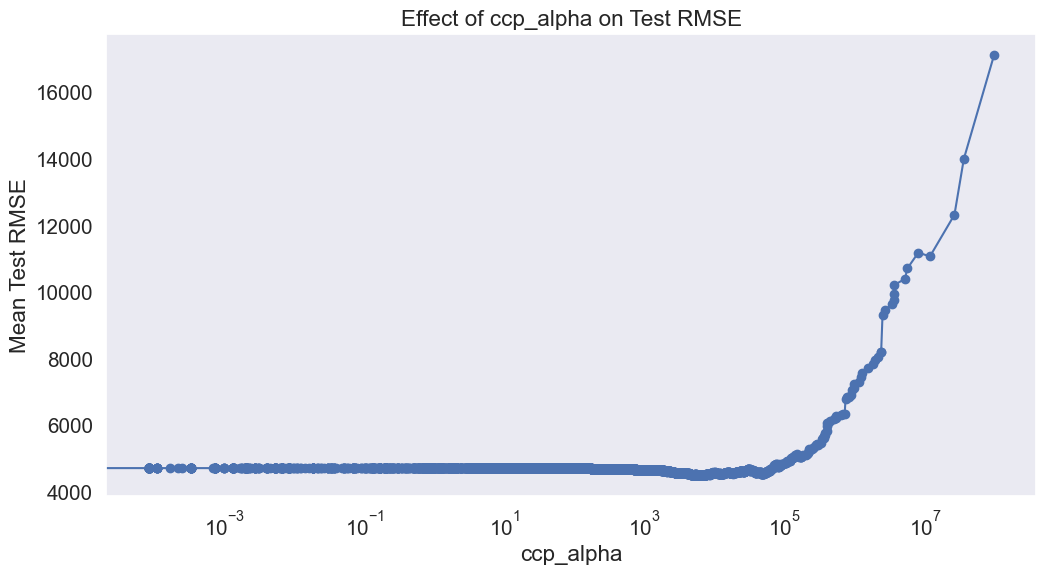
\includegraphics[keepaspectratio]{regression_tree_sp25_files/figure-pdf/cell-35-output-1.png}}

\chapter{Classification trees}\label{classification-trees}

\emph{Read section 8.1.2 of the book before using these notes.}

\emph{Note that in this course, lecture notes are not sufficient, you
must read the book for better understanding. Lecture notes are just
implementing the concepts of the book on a dataset, but not explaining
the concepts elaborately.}

Import libraries

\begin{Shaded}
\begin{Highlighting}[]
\CommentTok{\# \%load ../standard\_import.txt}
\ImportTok{import}\NormalTok{ pandas }\ImportTok{as}\NormalTok{ pd}
\ImportTok{import}\NormalTok{ numpy }\ImportTok{as}\NormalTok{ np}
\ImportTok{import}\NormalTok{ matplotlib.pyplot }\ImportTok{as}\NormalTok{ plt}
\ImportTok{import}\NormalTok{ seaborn }\ImportTok{as}\NormalTok{ sns}

\ImportTok{from}\NormalTok{ IPython.display }\ImportTok{import}\NormalTok{ Image}

\ImportTok{from}\NormalTok{ sklearn.model\_selection }\ImportTok{import}\NormalTok{ train\_test\_split, cross\_val\_score}
\ImportTok{from}\NormalTok{ six }\ImportTok{import}\NormalTok{ StringIO}
\ImportTok{from}\NormalTok{ sklearn.tree }\ImportTok{import}\NormalTok{ export\_graphviz, DecisionTreeClassifier, plot\_tree}
\ImportTok{from}\NormalTok{ sklearn.metrics }\ImportTok{import}\NormalTok{ confusion\_matrix, accuracy\_score}

\OperatorTok{\%}\NormalTok{matplotlib inline}
\end{Highlighting}
\end{Shaded}

\begin{Shaded}
\begin{Highlighting}[]
\CommentTok{\# load the dataset}
\NormalTok{heart\_df  }\OperatorTok{=}\NormalTok{ pd.read\_csv(}\StringTok{\textquotesingle{}datasets/heart\_disease\_classification.csv\textquotesingle{}}\NormalTok{)}
\BuiltInTok{print}\NormalTok{(heart\_df .shape)}
\NormalTok{heart\_df .head()}
\end{Highlighting}
\end{Shaded}

\begin{verbatim}
(303, 14)
\end{verbatim}

\begin{longtable}[]{@{}lllllllllllllll@{}}
\toprule\noalign{}
& age & sex & cp & trestbps & chol & fbs & restecg & thalach & exang &
oldpeak & slope & ca & thal & target \\
\midrule\noalign{}
\endhead
\bottomrule\noalign{}
\endlastfoot
0 & 63 & 1 & 3 & 145 & 233 & 1 & 0 & 150 & 0 & 2.3 & 0 & 0 & 1 & 1 \\
1 & 37 & 1 & 2 & 130 & 250 & 0 & 1 & 187 & 0 & 3.5 & 0 & 0 & 2 & 1 \\
2 & 41 & 0 & 1 & 130 & 204 & 0 & 0 & 172 & 0 & 1.4 & 2 & 0 & 2 & 1 \\
3 & 56 & 1 & 1 & 120 & 236 & 0 & 1 & 178 & 0 & 0.8 & 2 & 0 & 2 & 1 \\
4 & 57 & 0 & 0 & 120 & 354 & 0 & 1 & 163 & 1 & 0.6 & 2 & 0 & 2 & 1 \\
\end{longtable}

\begin{Shaded}
\begin{Highlighting}[]
\CommentTok{\# print out target distribution}
\NormalTok{heart\_df.target.value\_counts()}
\end{Highlighting}
\end{Shaded}

\begin{verbatim}
target
1    165
0    138
Name: count, dtype: int64
\end{verbatim}

\begin{Shaded}
\begin{Highlighting}[]
\CommentTok{\# split the x and y data}
\NormalTok{X }\OperatorTok{=}\NormalTok{ heart\_df.drop(columns}\OperatorTok{=}\NormalTok{[}\StringTok{\textquotesingle{}target\textquotesingle{}}\NormalTok{])}
\NormalTok{y }\OperatorTok{=}\NormalTok{ heart\_df.target}

\CommentTok{\# split the data into train and test sets}
\NormalTok{X\_train, X\_test, y\_train, y\_test }\OperatorTok{=}\NormalTok{ train\_test\_split(X, y, test\_size}\OperatorTok{=}\FloatTok{0.2}\NormalTok{, random\_state}\OperatorTok{=}\DecValTok{42}\NormalTok{)}
\end{Highlighting}
\end{Shaded}

\section{Building a Classification
Tree}\label{building-a-classification-tree}

We will build a classification tree to predict whether a person has
heart disease, using the default parameters of the decision tree
classifier.

\begin{Shaded}
\begin{Highlighting}[]
\CommentTok{\# create a decision tree classifier}
\NormalTok{tree }\OperatorTok{=}\NormalTok{ DecisionTreeClassifier(random\_state}\OperatorTok{=}\DecValTok{42}\NormalTok{)}

\CommentTok{\# fit the model to the training data}
\NormalTok{tree.fit(X\_train, y\_train)}

\CommentTok{\# make predictions on the test data}
\NormalTok{y\_pred }\OperatorTok{=}\NormalTok{ tree.predict(X\_test)}

\CommentTok{\# calculate the accuracy of the model}
\NormalTok{accuracy }\OperatorTok{=}\NormalTok{ accuracy\_score(y\_test, y\_pred)}
\BuiltInTok{print}\NormalTok{(}\SpecialStringTok{f\textquotesingle{}Test Accuracy: }\SpecialCharTok{\{}\NormalTok{accuracy}\SpecialCharTok{:.2f\}}\SpecialStringTok{\textquotesingle{}}\NormalTok{)}

\CommentTok{\# train accuracy}
\NormalTok{y\_train\_pred }\OperatorTok{=}\NormalTok{ tree.predict(X\_train)}
\NormalTok{train\_accuracy }\OperatorTok{=}\NormalTok{ accuracy\_score(y\_train, y\_train\_pred)}
\BuiltInTok{print}\NormalTok{(}\SpecialStringTok{f\textquotesingle{}Train Accuracy: }\SpecialCharTok{\{}\NormalTok{train\_accuracy}\SpecialCharTok{:.2f\}}\SpecialStringTok{\textquotesingle{}}\NormalTok{)}
\end{Highlighting}
\end{Shaded}

\begin{verbatim}
Test Accuracy: 0.75
Train Accuracy: 1.00
\end{verbatim}

\begin{Shaded}
\begin{Highlighting}[]
\CommentTok{\# plot the decision tree}
\NormalTok{plt.figure(figsize}\OperatorTok{=}\NormalTok{(}\DecValTok{12}\NormalTok{, }\DecValTok{8}\NormalTok{))}
\NormalTok{plot\_tree(tree, filled}\OperatorTok{=}\VariableTok{True}\NormalTok{, feature\_names}\OperatorTok{=}\NormalTok{X.columns, class\_names}\OperatorTok{=}\NormalTok{[}\StringTok{\textquotesingle{}No Disease\textquotesingle{}}\NormalTok{, }\StringTok{\textquotesingle{}Disease\textquotesingle{}}\NormalTok{])}
\NormalTok{plt.title(}\StringTok{\textquotesingle{}Decision Tree for Heart Disease Classification\textquotesingle{}}\NormalTok{)}\OperatorTok{;}
\end{Highlighting}
\end{Shaded}

\pandocbounded{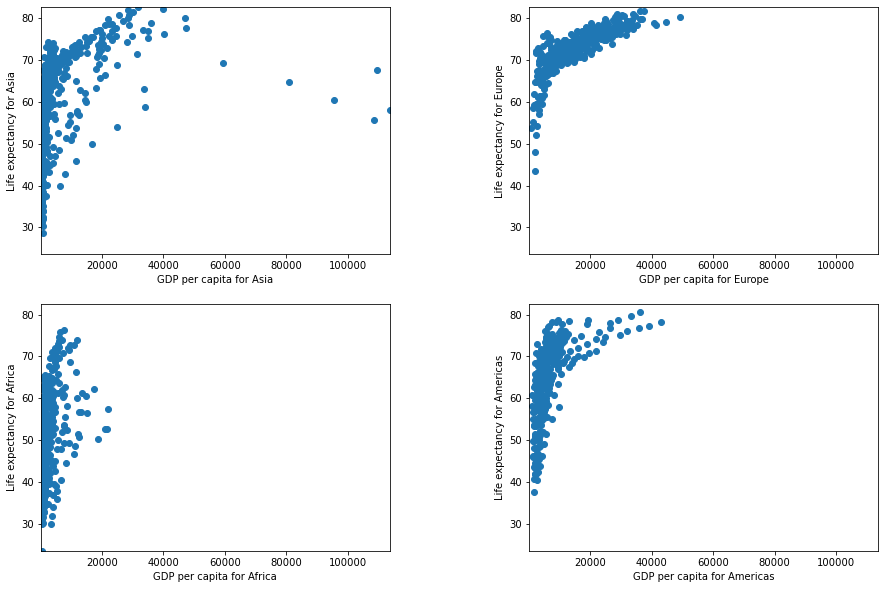
\includegraphics[keepaspectratio]{Classification _Tree_files/figure-pdf/cell-7-output-1.png}}

\begin{Shaded}
\begin{Highlighting}[]
\CommentTok{\# get the number of leaves in the tree}
\NormalTok{num\_leaves }\OperatorTok{=}\NormalTok{ tree.get\_n\_leaves()}
\BuiltInTok{print}\NormalTok{(}\SpecialStringTok{f\textquotesingle{}Number of leaves: }\SpecialCharTok{\{}\NormalTok{num\_leaves}\SpecialCharTok{\}}\SpecialStringTok{\textquotesingle{}}\NormalTok{)}

\CommentTok{\# get the depth of the tree}
\NormalTok{tree\_depth }\OperatorTok{=}\NormalTok{ tree.get\_depth()}
\BuiltInTok{print}\NormalTok{(}\SpecialStringTok{f\textquotesingle{}Depth of the tree: }\SpecialCharTok{\{}\NormalTok{tree\_depth}\SpecialCharTok{\}}\SpecialStringTok{\textquotesingle{}}\NormalTok{)}
\end{Highlighting}
\end{Shaded}

\begin{verbatim}
Number of leaves: 41
Depth of the tree: 9
\end{verbatim}

Clearly, the model is overfitting, as indicated by a training accuracy
of 100\% and a much lower test accuracy of 75\%.\\
Next, we will explore different strategies to address and reduce
overfitting.

\section{Pre-pruning: Hyperparameters
Tuning}\label{pre-pruning-hyperparameters-tuning}

Maximum depth of tree (\texttt{max\_depth}) - Used to control
over-fitting as higher depth will allow model to learn relations very
specific to a particular sample.

Minimum samples for a node split (\texttt{min\_samples\_split}) -
Defines the minimum number of samples (or observations) which are
required in a node to be considered for splitting. - Used to control
over-fitting. Higher values prevent a model from learning relations
which might be highly specific to the particular sample selected for a
tree.

Minimum samples for a terminal node (\texttt{min\_samples\_leaf}) -
Defines the minimum samples (or observations) required in a terminal
node or leaf. - Used to control over-fitting similar to
\texttt{min\_samples\_split}. - Generally lower values should be chosen
for imbalanced class problems because the regions in which the minority
class will be in majority will be very small.

Maximum number of terminal nodes (\texttt{max\_leaf\_nodes}) - The
maximum number of terminal nodes or leaves in a tree.

\begin{Shaded}
\begin{Highlighting}[]
\CommentTok{\# hyperparameter tuning}

\ImportTok{from}\NormalTok{ sklearn.model\_selection }\ImportTok{import}\NormalTok{ GridSearchCV}

\CommentTok{\# define the parameter grid}
\NormalTok{param\_grid }\OperatorTok{=}\NormalTok{ \{}
    \StringTok{\textquotesingle{}max\_depth\textquotesingle{}}\NormalTok{: }\BuiltInTok{list}\NormalTok{(}\BuiltInTok{range}\NormalTok{(}\DecValTok{1}\NormalTok{, }\DecValTok{9}\NormalTok{)) }\OperatorTok{+}\NormalTok{ [}\VariableTok{None}\NormalTok{], }
    \StringTok{\textquotesingle{}min\_samples\_split\textquotesingle{}}\NormalTok{: [}\DecValTok{2}\NormalTok{, }\DecValTok{5}\NormalTok{, }\DecValTok{10}\NormalTok{, }\DecValTok{15}\NormalTok{, }\DecValTok{20}\NormalTok{],}
    \StringTok{\textquotesingle{}min\_samples\_leaf\textquotesingle{}}\NormalTok{: [}\DecValTok{1}\NormalTok{, }\DecValTok{2}\NormalTok{, }\DecValTok{4}\NormalTok{]}
\NormalTok{\}}

\CommentTok{\# create a grid search object}
\NormalTok{grid\_search }\OperatorTok{=}\NormalTok{ GridSearchCV(estimator}\OperatorTok{=}\NormalTok{tree, param\_grid}\OperatorTok{=}\NormalTok{param\_grid, cv}\OperatorTok{=}\DecValTok{5}\NormalTok{, n\_jobs}\OperatorTok{={-}}\DecValTok{1}\NormalTok{, verbose}\OperatorTok{=}\DecValTok{2}\NormalTok{)}
\CommentTok{\# fit the grid search to the training data}
\NormalTok{grid\_search.fit(X\_train, y\_train)}
\CommentTok{\# print the best parameters}
\BuiltInTok{print}\NormalTok{(}\StringTok{"Best parameters found: "}\NormalTok{, grid\_search.best\_params\_)}

\CommentTok{\# print the best score}
\BuiltInTok{print}\NormalTok{(}\StringTok{"Best score: "}\NormalTok{, grid\_search.best\_score\_)}
\CommentTok{\# get the best estimator}
\NormalTok{best\_tree }\OperatorTok{=}\NormalTok{ grid\_search.best\_estimator\_}

\CommentTok{\# make predictions on the test data with the best estimator}
\NormalTok{y\_pred\_best }\OperatorTok{=}\NormalTok{ best\_tree.predict(X\_test)}
\CommentTok{\# calculate the accuracy of the best estimator}
\NormalTok{best\_accuracy }\OperatorTok{=}\NormalTok{ accuracy\_score(y\_test, y\_pred\_best)}
\BuiltInTok{print}\NormalTok{(}\SpecialStringTok{f\textquotesingle{}Best Test Accuracy: }\SpecialCharTok{\{}\NormalTok{best\_accuracy}\SpecialCharTok{:.2f\}}\SpecialStringTok{\textquotesingle{}}\NormalTok{)}
\end{Highlighting}
\end{Shaded}

\begin{verbatim}
Fitting 5 folds for each of 135 candidates, totalling 675 fits
Best parameters found:  {'max_depth': 6, 'min_samples_leaf': 2, 'min_samples_split': 10}
Best score:  0.7687074829931972
Best Test Accuracy: 0.85
\end{verbatim}

\begin{Shaded}
\begin{Highlighting}[]
\CommentTok{\# print out the best tree depth and number of leaves}
\NormalTok{best\_num\_leaves }\OperatorTok{=}\NormalTok{ best\_tree.get\_n\_leaves()}
\BuiltInTok{print}\NormalTok{(}\SpecialStringTok{f\textquotesingle{}Best Number of leaves: }\SpecialCharTok{\{}\NormalTok{best\_num\_leaves}\SpecialCharTok{\}}\SpecialStringTok{\textquotesingle{}}\NormalTok{)}

\NormalTok{best\_tree\_depth }\OperatorTok{=}\NormalTok{ best\_tree.get\_depth()}
\BuiltInTok{print}\NormalTok{(}\SpecialStringTok{f\textquotesingle{}Best Depth of the tree: }\SpecialCharTok{\{}\NormalTok{best\_tree\_depth}\SpecialCharTok{\}}\SpecialStringTok{\textquotesingle{}}\NormalTok{)}
\end{Highlighting}
\end{Shaded}

\begin{verbatim}
Best Number of leaves: 21
Best Depth of the tree: 6
\end{verbatim}

\begin{Shaded}
\begin{Highlighting}[]
\CommentTok{\# plot the best decision tree}
\NormalTok{plt.figure(figsize}\OperatorTok{=}\NormalTok{(}\DecValTok{12}\NormalTok{, }\DecValTok{8}\NormalTok{))}
\NormalTok{plot\_tree(best\_tree, filled}\OperatorTok{=}\VariableTok{True}\NormalTok{, feature\_names}\OperatorTok{=}\NormalTok{X.columns, class\_names}\OperatorTok{=}\NormalTok{[}\StringTok{\textquotesingle{}No Disease\textquotesingle{}}\NormalTok{, }\StringTok{\textquotesingle{}Disease\textquotesingle{}}\NormalTok{])}
\NormalTok{plt.title(}\StringTok{\textquotesingle{}Best Decision Tree for Heart Disease Classification\textquotesingle{}}\NormalTok{)}
\NormalTok{plt.show()}
\end{Highlighting}
\end{Shaded}

\pandocbounded{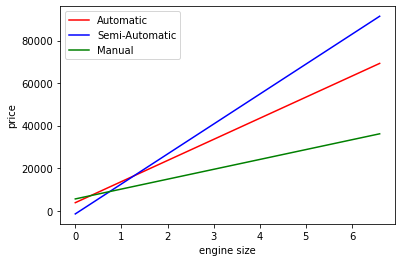
\includegraphics[keepaspectratio]{Classification _Tree_files/figure-pdf/cell-11-output-1.png}}

\subsection{Gini or entropy}\label{gini-or-entropy}

\begin{Shaded}
\begin{Highlighting}[]
\CommentTok{\# define the parameter grid}
\NormalTok{param\_grid\_metric }\OperatorTok{=}\NormalTok{ \{}
    \StringTok{\textquotesingle{}max\_depth\textquotesingle{}}\NormalTok{: }\BuiltInTok{list}\NormalTok{(}\BuiltInTok{range}\NormalTok{(}\DecValTok{1}\NormalTok{, }\DecValTok{9}\NormalTok{)) }\OperatorTok{+}\NormalTok{ [}\VariableTok{None}\NormalTok{], }
    \StringTok{\textquotesingle{}min\_samples\_split\textquotesingle{}}\NormalTok{: [}\DecValTok{2}\NormalTok{, }\DecValTok{5}\NormalTok{, }\DecValTok{10}\NormalTok{, }\DecValTok{15}\NormalTok{, }\DecValTok{20}\NormalTok{],}
    \StringTok{\textquotesingle{}min\_samples\_leaf\textquotesingle{}}\NormalTok{: [}\DecValTok{1}\NormalTok{, }\DecValTok{2}\NormalTok{, }\DecValTok{4}\NormalTok{],}
    \CommentTok{\# adding the criterion parameter to the grid search}
    \StringTok{\textquotesingle{}criterion\textquotesingle{}}\NormalTok{: [}\StringTok{\textquotesingle{}gini\textquotesingle{}}\NormalTok{, }\StringTok{\textquotesingle{}entropy\textquotesingle{}}\NormalTok{]}
\NormalTok{\}}

\CommentTok{\# create a grid search object}
\NormalTok{grid\_search\_metric }\OperatorTok{=}\NormalTok{ GridSearchCV(estimator}\OperatorTok{=}\NormalTok{tree, param\_grid}\OperatorTok{=}\NormalTok{param\_grid\_metric, cv}\OperatorTok{=}\DecValTok{5}\NormalTok{, n\_jobs}\OperatorTok{={-}}\DecValTok{1}\NormalTok{, verbose}\OperatorTok{=}\DecValTok{2}\NormalTok{)}
\CommentTok{\# fit the grid search to the training data}
\NormalTok{grid\_search\_metric.fit(X\_train, y\_train)}
\CommentTok{\# print the best parameters}
\BuiltInTok{print}\NormalTok{(}\StringTok{"Best parameters found: "}\NormalTok{, grid\_search\_metric.best\_params\_)}

\CommentTok{\# print the best score}
\BuiltInTok{print}\NormalTok{(}\StringTok{"Best score: "}\NormalTok{, grid\_search\_metric.best\_score\_)}
\CommentTok{\# get the best estimator}
\NormalTok{best\_tree }\OperatorTok{=}\NormalTok{ grid\_search\_metric.best\_estimator\_}

\CommentTok{\# make predictions on the test data with the best estimator}
\NormalTok{y\_pred\_best }\OperatorTok{=}\NormalTok{ best\_tree.predict(X\_test)}
\CommentTok{\# calculate the accuracy of the best estimator}
\NormalTok{best\_accuracy }\OperatorTok{=}\NormalTok{ accuracy\_score(y\_test, y\_pred\_best)}
\BuiltInTok{print}\NormalTok{(}\SpecialStringTok{f\textquotesingle{}Best Test Accuracy: }\SpecialCharTok{\{}\NormalTok{best\_accuracy}\SpecialCharTok{:.2f\}}\SpecialStringTok{\textquotesingle{}}\NormalTok{)}
\end{Highlighting}
\end{Shaded}

\begin{verbatim}
Fitting 5 folds for each of 270 candidates, totalling 1350 fits
Best parameters found:  {'criterion': 'entropy', 'max_depth': 4, 'min_samples_leaf': 1, 'min_samples_split': 20}
Best score:  0.7811224489795918
Best Test Accuracy: 0.85
\end{verbatim}

\begin{Shaded}
\begin{Highlighting}[]
\CommentTok{\# print out the best tree depth and number of leaves}
\NormalTok{best\_num\_leaves }\OperatorTok{=}\NormalTok{ best\_tree.get\_n\_leaves()}
\BuiltInTok{print}\NormalTok{(}\SpecialStringTok{f\textquotesingle{}Best Number of leaves: }\SpecialCharTok{\{}\NormalTok{best\_num\_leaves}\SpecialCharTok{\}}\SpecialStringTok{\textquotesingle{}}\NormalTok{)}

\NormalTok{best\_tree\_depth }\OperatorTok{=}\NormalTok{ best\_tree.get\_depth()}
\BuiltInTok{print}\NormalTok{(}\SpecialStringTok{f\textquotesingle{}Best Depth of the tree: }\SpecialCharTok{\{}\NormalTok{best\_tree\_depth}\SpecialCharTok{\}}\SpecialStringTok{\textquotesingle{}}\NormalTok{)}
\end{Highlighting}
\end{Shaded}

\begin{verbatim}
Best Number of leaves: 11
Best Depth of the tree: 4
\end{verbatim}

\begin{Shaded}
\begin{Highlighting}[]
\CommentTok{\# plot the best decision tree}
\NormalTok{plt.figure(figsize}\OperatorTok{=}\NormalTok{(}\DecValTok{12}\NormalTok{, }\DecValTok{8}\NormalTok{))}
\NormalTok{plot\_tree(best\_tree, filled}\OperatorTok{=}\VariableTok{True}\NormalTok{, feature\_names}\OperatorTok{=}\NormalTok{X.columns, class\_names}\OperatorTok{=}\NormalTok{[}\StringTok{\textquotesingle{}No Disease\textquotesingle{}}\NormalTok{, }\StringTok{\textquotesingle{}Disease\textquotesingle{}}\NormalTok{])}
\NormalTok{plt.title(}\StringTok{\textquotesingle{}Best Decision Tree for Heart Disease Classification\textquotesingle{}}\NormalTok{)}
\NormalTok{plt.show()}
\end{Highlighting}
\end{Shaded}

\pandocbounded{\includegraphics[keepaspectratio]{Classification _Tree_files/figure-pdf/cell-14-output-1.png}}

Both criteria aim to minimize impurity in splits, in pratice, they often
lead to comparable performance in decision trees, even though their
mathematical forulations differ

\begin{itemize}
\tightlist
\item
  \textbf{Gini}: Faster to compute (no logarithms) and often used for
  large datasets. so it is a good default. May produce slightly more
  complex trees.
\item
  \textbf{Entropy}: Slower but aligns with information theory. Prefers
  splits that balance node sizes, leading to more interpretable trees.
\end{itemize}

\section{Post-pruning: Cost complexity
pruning}\label{post-pruning-cost-complexity-pruning}

Post-pruning, on the other hand, allows the decision tree to grow to its
full extent and then prunes it back to reduce complexity. This approach
first builds a complete tree and then removes or collapses branches that
don't significantly contribute to the model's performance. One common
post-pruning technique is called Cost-Complexity Pruning.

\subsection{step 1: calculate the cost complexity pruning
path}\label{step-1-calculate-the-cost-complexity-pruning-path}

\begin{Shaded}
\begin{Highlighting}[]
\NormalTok{path }\OperatorTok{=}\NormalTok{ tree.cost\_complexity\_pruning\_path(X\_train, y\_train)}
\NormalTok{ccp\_alphas, impurities }\OperatorTok{=}\NormalTok{ path.ccp\_alphas, path.impurities}
\end{Highlighting}
\end{Shaded}

\subsection{step 2: Create trees with different ccp\_alpha values and
evaluate their
performance}\label{step-2-create-trees-with-different-ccp_alpha-values-and-evaluate-their-performance}

\begin{Shaded}
\begin{Highlighting}[]

\CommentTok{\# We\textquotesingle{}ll skip the last alpha which would produce a single{-}node tree}
\NormalTok{alphas }\OperatorTok{=}\NormalTok{ ccp\_alphas[:}\OperatorTok{{-}}\DecValTok{1}\NormalTok{]}

\CommentTok{\# Create empty lists to store the results}
\NormalTok{train\_scores }\OperatorTok{=}\NormalTok{ []}
\NormalTok{test\_scores }\OperatorTok{=}\NormalTok{ []}
\NormalTok{cv\_scores }\OperatorTok{=}\NormalTok{ []}
\NormalTok{node\_counts }\OperatorTok{=}\NormalTok{ []}

\CommentTok{\# For each alpha value, fit a tree and evaluate}
\ControlFlowTok{for}\NormalTok{ alpha }\KeywordTok{in}\NormalTok{ alphas:}
    \CommentTok{\# Create and train the model}
\NormalTok{    clf }\OperatorTok{=}\NormalTok{ DecisionTreeClassifier(ccp\_alpha}\OperatorTok{=}\NormalTok{alpha, random\_state}\OperatorTok{=}\DecValTok{42}\NormalTok{)}
\NormalTok{    clf.fit(X\_train, y\_train)}
    
    \CommentTok{\# Record scores}
\NormalTok{    train\_scores.append(accuracy\_score(y\_train, clf.predict(X\_train)))}
\NormalTok{    test\_scores.append(accuracy\_score(y\_test, clf.predict(X\_test)))}
    
    \CommentTok{\# Cross{-}validation score for robustness}
\NormalTok{    cv\_score }\OperatorTok{=}\NormalTok{ cross\_val\_score(clf, X\_train, y\_train, cv}\OperatorTok{=}\DecValTok{5}\NormalTok{).mean()}
\NormalTok{    cv\_scores.append(cv\_score)}
    
    \CommentTok{\# Record tree complexity}
\NormalTok{    node\_counts.append(clf.tree\_.node\_count)}
\end{Highlighting}
\end{Shaded}

\subsection{Step 3: Visualize the
results}\label{step-3-visualize-the-results}

\begin{Shaded}
\begin{Highlighting}[]
\CommentTok{\# Step 3: Visualize the results}
\NormalTok{fig, ax }\OperatorTok{=}\NormalTok{ plt.subplots(}\DecValTok{2}\NormalTok{, }\DecValTok{2}\NormalTok{, figsize}\OperatorTok{=}\NormalTok{(}\DecValTok{15}\NormalTok{, }\DecValTok{10}\NormalTok{))}

\CommentTok{\# Plot accuracy vs alpha}
\NormalTok{ax[}\DecValTok{0}\NormalTok{, }\DecValTok{0}\NormalTok{].plot(alphas, train\_scores, marker}\OperatorTok{=}\StringTok{\textquotesingle{}o\textquotesingle{}}\NormalTok{, label}\OperatorTok{=}\StringTok{\textquotesingle{}Train\textquotesingle{}}\NormalTok{)}
\NormalTok{ax[}\DecValTok{0}\NormalTok{, }\DecValTok{0}\NormalTok{].plot(alphas, test\_scores, marker}\OperatorTok{=}\StringTok{\textquotesingle{}o\textquotesingle{}}\NormalTok{, label}\OperatorTok{=}\StringTok{\textquotesingle{}Test\textquotesingle{}}\NormalTok{)}
\NormalTok{ax[}\DecValTok{0}\NormalTok{, }\DecValTok{0}\NormalTok{].plot(alphas, cv\_scores, marker}\OperatorTok{=}\StringTok{\textquotesingle{}o\textquotesingle{}}\NormalTok{, label}\OperatorTok{=}\StringTok{\textquotesingle{}Cross{-}validation\textquotesingle{}}\NormalTok{)}
\NormalTok{ax[}\DecValTok{0}\NormalTok{, }\DecValTok{0}\NormalTok{].set\_xlabel(}\StringTok{\textquotesingle{}ccp\_alpha\textquotesingle{}}\NormalTok{)}
\NormalTok{ax[}\DecValTok{0}\NormalTok{, }\DecValTok{0}\NormalTok{].set\_ylabel(}\StringTok{\textquotesingle{}Accuracy\textquotesingle{}}\NormalTok{)}
\NormalTok{ax[}\DecValTok{0}\NormalTok{, }\DecValTok{0}\NormalTok{].set\_title(}\StringTok{\textquotesingle{}Accuracy vs. ccp\_alpha\textquotesingle{}}\NormalTok{)}
\NormalTok{ax[}\DecValTok{0}\NormalTok{, }\DecValTok{0}\NormalTok{].legend()}
\NormalTok{ax[}\DecValTok{0}\NormalTok{, }\DecValTok{0}\NormalTok{].grid(}\VariableTok{True}\NormalTok{)}

\CommentTok{\# Plot number of nodes vs alpha}
\NormalTok{ax[}\DecValTok{0}\NormalTok{, }\DecValTok{1}\NormalTok{].plot(alphas, node\_counts, marker}\OperatorTok{=}\StringTok{\textquotesingle{}o\textquotesingle{}}\NormalTok{)}
\NormalTok{ax[}\DecValTok{0}\NormalTok{, }\DecValTok{1}\NormalTok{].set\_xlabel(}\StringTok{\textquotesingle{}ccp\_alpha\textquotesingle{}}\NormalTok{)}
\NormalTok{ax[}\DecValTok{0}\NormalTok{, }\DecValTok{1}\NormalTok{].set\_ylabel(}\StringTok{\textquotesingle{}Number of nodes\textquotesingle{}}\NormalTok{)}
\NormalTok{ax[}\DecValTok{0}\NormalTok{, }\DecValTok{1}\NormalTok{].set\_title(}\StringTok{\textquotesingle{}Tree complexity vs. ccp\_alpha\textquotesingle{}}\NormalTok{)}
\NormalTok{ax[}\DecValTok{0}\NormalTok{, }\DecValTok{1}\NormalTok{].grid(}\VariableTok{True}\NormalTok{)}

\CommentTok{\# Log scale for better visualization of small alpha values}
\NormalTok{ax[}\DecValTok{1}\NormalTok{, }\DecValTok{0}\NormalTok{].plot(alphas, train\_scores, marker}\OperatorTok{=}\StringTok{\textquotesingle{}o\textquotesingle{}}\NormalTok{, label}\OperatorTok{=}\StringTok{\textquotesingle{}Train\textquotesingle{}}\NormalTok{)}
\NormalTok{ax[}\DecValTok{1}\NormalTok{, }\DecValTok{0}\NormalTok{].plot(alphas, test\_scores, marker}\OperatorTok{=}\StringTok{\textquotesingle{}o\textquotesingle{}}\NormalTok{, label}\OperatorTok{=}\StringTok{\textquotesingle{}Test\textquotesingle{}}\NormalTok{)}
\NormalTok{ax[}\DecValTok{1}\NormalTok{, }\DecValTok{0}\NormalTok{].plot(alphas, cv\_scores, marker}\OperatorTok{=}\StringTok{\textquotesingle{}o\textquotesingle{}}\NormalTok{, label}\OperatorTok{=}\StringTok{\textquotesingle{}Cross{-}validation\textquotesingle{}}\NormalTok{)}
\NormalTok{ax[}\DecValTok{1}\NormalTok{, }\DecValTok{0}\NormalTok{].set\_xlabel(}\StringTok{\textquotesingle{}ccp\_alpha (log scale)\textquotesingle{}}\NormalTok{)}
\NormalTok{ax[}\DecValTok{1}\NormalTok{, }\DecValTok{0}\NormalTok{].set\_ylabel(}\StringTok{\textquotesingle{}Accuracy\textquotesingle{}}\NormalTok{)}
\NormalTok{ax[}\DecValTok{1}\NormalTok{, }\DecValTok{0}\NormalTok{].set\_title(}\StringTok{\textquotesingle{}Accuracy vs. ccp\_alpha (log scale)\textquotesingle{}}\NormalTok{)}
\NormalTok{ax[}\DecValTok{1}\NormalTok{, }\DecValTok{0}\NormalTok{].set\_xscale(}\StringTok{\textquotesingle{}log\textquotesingle{}}\NormalTok{)}
\NormalTok{ax[}\DecValTok{1}\NormalTok{, }\DecValTok{0}\NormalTok{].legend()}
\NormalTok{ax[}\DecValTok{1}\NormalTok{, }\DecValTok{0}\NormalTok{].grid(}\VariableTok{True}\NormalTok{)}

\CommentTok{\# Find best alpha based on test score}
\NormalTok{best\_test\_idx }\OperatorTok{=}\NormalTok{ np.argmax(test\_scores)}
\NormalTok{best\_test\_alpha }\OperatorTok{=}\NormalTok{ alphas[best\_test\_idx]}
\NormalTok{best\_test\_acc }\OperatorTok{=}\NormalTok{ test\_scores[best\_test\_idx]}

\CommentTok{\# Find best alpha based on CV score (more robust)}
\NormalTok{best\_cv\_idx }\OperatorTok{=}\NormalTok{ np.argmax(cv\_scores)}
\NormalTok{best\_cv\_alpha }\OperatorTok{=}\NormalTok{ alphas[best\_cv\_idx]}
\NormalTok{best\_cv\_acc }\OperatorTok{=}\NormalTok{ cv\_scores[best\_cv\_idx]}

\CommentTok{\# Plot highlighting best points}
\NormalTok{ax[}\DecValTok{1}\NormalTok{, }\DecValTok{1}\NormalTok{].plot(alphas, test\_scores, }\StringTok{\textquotesingle{}b{-}\textquotesingle{}}\NormalTok{, marker}\OperatorTok{=}\StringTok{\textquotesingle{}o\textquotesingle{}}\NormalTok{, label}\OperatorTok{=}\StringTok{\textquotesingle{}Test accuracy\textquotesingle{}}\NormalTok{)}
\NormalTok{ax[}\DecValTok{1}\NormalTok{, }\DecValTok{1}\NormalTok{].plot(alphas, cv\_scores, }\StringTok{\textquotesingle{}g{-}\textquotesingle{}}\NormalTok{, marker}\OperatorTok{=}\StringTok{\textquotesingle{}o\textquotesingle{}}\NormalTok{, label}\OperatorTok{=}\StringTok{\textquotesingle{}CV accuracy\textquotesingle{}}\NormalTok{)}
\NormalTok{ax[}\DecValTok{1}\NormalTok{, }\DecValTok{1}\NormalTok{].axvline(x}\OperatorTok{=}\NormalTok{best\_test\_alpha, color}\OperatorTok{=}\StringTok{\textquotesingle{}blue\textquotesingle{}}\NormalTok{, linestyle}\OperatorTok{=}\StringTok{\textquotesingle{}{-}{-}\textquotesingle{}}\NormalTok{, alpha}\OperatorTok{=}\FloatTok{0.5}\NormalTok{, }
\NormalTok{                label}\OperatorTok{=}\SpecialStringTok{f\textquotesingle{}Best test alpha: }\SpecialCharTok{\{}\NormalTok{best\_test\_alpha}\SpecialCharTok{:.6f\}}\SpecialStringTok{\textquotesingle{}}\NormalTok{)}
\NormalTok{ax[}\DecValTok{1}\NormalTok{, }\DecValTok{1}\NormalTok{].axvline(x}\OperatorTok{=}\NormalTok{best\_cv\_alpha, color}\OperatorTok{=}\StringTok{\textquotesingle{}green\textquotesingle{}}\NormalTok{, linestyle}\OperatorTok{=}\StringTok{\textquotesingle{}{-}{-}\textquotesingle{}}\NormalTok{, alpha}\OperatorTok{=}\FloatTok{0.5}\NormalTok{,}
\NormalTok{                label}\OperatorTok{=}\SpecialStringTok{f\textquotesingle{}Best CV alpha: }\SpecialCharTok{\{}\NormalTok{best\_cv\_alpha}\SpecialCharTok{:.6f\}}\SpecialStringTok{\textquotesingle{}}\NormalTok{)}
\NormalTok{ax[}\DecValTok{1}\NormalTok{, }\DecValTok{1}\NormalTok{].set\_xlabel(}\StringTok{\textquotesingle{}ccp\_alpha\textquotesingle{}}\NormalTok{)}
\NormalTok{ax[}\DecValTok{1}\NormalTok{, }\DecValTok{1}\NormalTok{].set\_ylabel(}\StringTok{\textquotesingle{}Accuracy\textquotesingle{}}\NormalTok{)}
\NormalTok{ax[}\DecValTok{1}\NormalTok{, }\DecValTok{1}\NormalTok{].set\_title(}\StringTok{\textquotesingle{}Finding optimal ccp\_alpha\textquotesingle{}}\NormalTok{)}
\NormalTok{ax[}\DecValTok{1}\NormalTok{, }\DecValTok{1}\NormalTok{].legend(loc}\OperatorTok{=}\StringTok{\textquotesingle{}lower left\textquotesingle{}}\NormalTok{)}
\NormalTok{ax[}\DecValTok{1}\NormalTok{, }\DecValTok{1}\NormalTok{].grid(}\VariableTok{True}\NormalTok{)}

\NormalTok{plt.tight\_layout()}
\NormalTok{plt.show()}

\CommentTok{\# Print the optimal alpha values and corresponding metrics}
\BuiltInTok{print}\NormalTok{(}\SpecialStringTok{f"Best alpha based on test score: }\SpecialCharTok{\{}\NormalTok{best\_test\_alpha}\SpecialCharTok{:.6f\}}\SpecialStringTok{ (Accuracy: }\SpecialCharTok{\{}\NormalTok{best\_test\_acc}\SpecialCharTok{:.4f\}}\SpecialStringTok{, Nodes: }\SpecialCharTok{\{}\NormalTok{node\_counts[best\_test\_idx]}\SpecialCharTok{\}}\SpecialStringTok{)"}\NormalTok{)}
\BuiltInTok{print}\NormalTok{(}\SpecialStringTok{f"Best alpha based on CV score: }\SpecialCharTok{\{}\NormalTok{best\_cv\_alpha}\SpecialCharTok{:.6f\}}\SpecialStringTok{ (Accuracy: }\SpecialCharTok{\{}\NormalTok{best\_cv\_acc}\SpecialCharTok{:.4f\}}\SpecialStringTok{, Nodes: }\SpecialCharTok{\{}\NormalTok{node\_counts[best\_cv\_idx]}\SpecialCharTok{\}}\SpecialStringTok{)"}\NormalTok{)}
\end{Highlighting}
\end{Shaded}

\pandocbounded{\includegraphics[keepaspectratio]{Classification _Tree_files/figure-pdf/cell-17-output-1.png}}

\subsection{Step 4: Create the final model with the optimal
alpha}\label{step-4-create-the-final-model-with-the-optimal-alpha}

\begin{Shaded}
\begin{Highlighting}[]
\CommentTok{\# Using CV{-}based alpha as it\textquotesingle{}s more robust against overfitting}
\NormalTok{final\_model }\OperatorTok{=}\NormalTok{ DecisionTreeClassifier(ccp\_alpha}\OperatorTok{=}\NormalTok{best\_cv\_alpha, random\_state}\OperatorTok{=}\DecValTok{42}\NormalTok{)}
\NormalTok{final\_model.fit(X\_train, y\_train)}

\CommentTok{\# Evaluate the final model}
\NormalTok{train\_acc }\OperatorTok{=}\NormalTok{ accuracy\_score(y\_train, final\_model.predict(X\_train))}
\NormalTok{test\_acc }\OperatorTok{=}\NormalTok{ accuracy\_score(y\_test, final\_model.predict(X\_test))}

\BuiltInTok{print}\NormalTok{(}\SpecialStringTok{f"}\CharTok{\textbackslash{}n}\SpecialStringTok{Final model performance:"}\NormalTok{)}
\BuiltInTok{print}\NormalTok{(}\SpecialStringTok{f"Training accuracy: }\SpecialCharTok{\{}\NormalTok{train\_acc}\SpecialCharTok{:.4f\}}\SpecialStringTok{"}\NormalTok{)}
\BuiltInTok{print}\NormalTok{(}\SpecialStringTok{f"Test accuracy: }\SpecialCharTok{\{}\NormalTok{test\_acc}\SpecialCharTok{:.4f\}}\SpecialStringTok{"}\NormalTok{)}
\BuiltInTok{print}\NormalTok{(}\SpecialStringTok{f"Tree nodes: }\SpecialCharTok{\{}\NormalTok{final\_model}\SpecialCharTok{.}\NormalTok{tree\_}\SpecialCharTok{.}\NormalTok{node\_count}\SpecialCharTok{\}}\SpecialStringTok{"}\NormalTok{)}
\BuiltInTok{print}\NormalTok{(}\SpecialStringTok{f"Tree depth: }\SpecialCharTok{\{}\NormalTok{final\_model}\SpecialCharTok{.}\NormalTok{get\_depth()}\SpecialCharTok{\}}\SpecialStringTok{"}\NormalTok{)}
\end{Highlighting}
\end{Shaded}

\begin{verbatim}
Best alpha based on test score: 0.007969 (Accuracy: 0.8852, Nodes: 23)
Best alpha based on CV score: 0.007969 (Accuracy: 0.7604, Nodes: 23)

Final model performance:
Training accuracy: 0.8967
Test accuracy: 0.8852
Tree nodes: 23
Tree depth: 6
\end{verbatim}

\begin{Shaded}
\begin{Highlighting}[]
\CommentTok{\# plot the final decision tree}
\NormalTok{plt.figure(figsize}\OperatorTok{=}\NormalTok{(}\DecValTok{12}\NormalTok{, }\DecValTok{8}\NormalTok{))}
\NormalTok{plot\_tree(final\_model, filled}\OperatorTok{=}\VariableTok{True}\NormalTok{, feature\_names}\OperatorTok{=}\NormalTok{X.columns, class\_names}\OperatorTok{=}\NormalTok{[}\StringTok{\textquotesingle{}No Disease\textquotesingle{}}\NormalTok{, }\StringTok{\textquotesingle{}Disease\textquotesingle{}}\NormalTok{])}
\NormalTok{plt.title(}\StringTok{\textquotesingle{}Final Decision Tree for Heart Disease Classification\textquotesingle{}}\NormalTok{)}
\NormalTok{plt.show()}
\end{Highlighting}
\end{Shaded}

\pandocbounded{\includegraphics[keepaspectratio]{Classification _Tree_files/figure-pdf/cell-19-output-1.png}}

Post-pruning can potentially create more optimal trees, as it considers
the entire tree structure before making pruning decisions. However, it
can be more computationally expensive.

Both approaches aim to find a balance between model complexity and
performance, with the goal of creating a model that generalizes well to
unseen data. The choice between pre-pruning and post-pruning (or a
combination of both) often depends on the specific dataset, the problem
at hand, and of course, computational resources available.

\section{Feature Importance in Decision
Trees}\label{feature-importance-in-decision-trees}

Decision tree algorithms, such as Classification and Regression Trees
(CART), compute \textbf{feature importance} scores based on how much
each feature contributes to reducing the splitting criterion (e.g.,
\textbf{Gini impurity} or \textbf{entropy}).

This methodology extends naturally to \textbf{ensemble models} like
\textbf{Random Forests} and \textbf{Gradient Boosting}, which average
feature importance across all trees in the ensemble.

Once a model is trained, the relative importance of each feature can be
accessed using the \texttt{.feature\_importances\_} attribute. These
scores indicate how valuable each feature was in constructing the
decision rules that led to the model's predictions.

\begin{Shaded}
\begin{Highlighting}[]
\NormalTok{importances  }\OperatorTok{=}\NormalTok{ final\_model.feature\_importances\_}

\CommentTok{\# Create a DataFrame for easier visualization}
\NormalTok{feature\_importance\_df }\OperatorTok{=}\NormalTok{ pd.DataFrame(\{}
    \StringTok{\textquotesingle{}Feature\textquotesingle{}}\NormalTok{: X.columns,}
    \StringTok{\textquotesingle{}Importance\textquotesingle{}}\NormalTok{: importances}
\NormalTok{\}).sort\_values(by}\OperatorTok{=}\StringTok{\textquotesingle{}Importance\textquotesingle{}}\NormalTok{, ascending}\OperatorTok{=}\VariableTok{False}\NormalTok{)}

\CommentTok{\# Display the DataFrame}
\NormalTok{feature\_importance\_df}
\end{Highlighting}
\end{Shaded}

\begin{longtable}[]{@{}lll@{}}
\toprule\noalign{}
& Feature & Importance \\
\midrule\noalign{}
\endhead
\bottomrule\noalign{}
\endlastfoot
2 & cp & 0.340102 \\
11 & ca & 0.145273 \\
9 & oldpeak & 0.139508 \\
8 & exang & 0.113871 \\
0 & age & 0.095885 \\
4 & chol & 0.056089 \\
10 & slope & 0.041242 \\
12 & thal & 0.035531 \\
1 & sex & 0.032499 \\
3 & trestbps & 0.000000 \\
5 & fbs & 0.000000 \\
6 & restecg & 0.000000 \\
7 & thalach & 0.000000 \\
\end{longtable}

\begin{Shaded}
\begin{Highlighting}[]
\NormalTok{plt.figure(figsize}\OperatorTok{=}\NormalTok{(}\DecValTok{10}\NormalTok{, }\DecValTok{6}\NormalTok{))}
\NormalTok{plt.barh(feature\_importance\_df[}\StringTok{\textquotesingle{}Feature\textquotesingle{}}\NormalTok{], feature\_importance\_df[}\StringTok{\textquotesingle{}Importance\textquotesingle{}}\NormalTok{])}
\NormalTok{plt.xlabel(}\StringTok{"Importance Score"}\NormalTok{)}
\NormalTok{plt.title(}\StringTok{"Feature Importances"}\NormalTok{)}
\NormalTok{plt.gca().invert\_yaxis()  }\CommentTok{\# Most important feature at the top}
\NormalTok{plt.show()}
\end{Highlighting}
\end{Shaded}

\pandocbounded{\includegraphics[keepaspectratio]{Classification _Tree_files/figure-pdf/cell-21-output-1.png}}

\subsection{Do We Need Feature Selection or Regularization with Tree
Models?}\label{do-we-need-feature-selection-or-regularization-with-tree-models}

When using \textbf{tree-based models} (e.g., Decision Trees, Random
Forests, Gradient Boosting) and you have a \textbf{small number of
predictors}, you typically \textbf{don't need to worry much about
feature selection or regularization}. Here's why:

\begin{itemize}
\tightlist
\item
  \textbf{Tree models inherently ignore uninformative features}. They
  only split on features that reduce impurity (e.g., Gini or entropy),
  so irrelevant features tend to receive \textbf{zero or very low
  importance}.
\item
  \textbf{Ensemble methods} like Random Forest or Boosting average over
  many trees. Features that don't help prediction are rarely used across
  the ensemble.
\item
  \textbf{Including unimportant features won't significantly hurt model
  performance} in small feature spaces. The model will usually ignore
  them during training.
\item
  \textbf{However}, even in small feature sets, irrelevant features may
  slightly:
\item
  Increase model variance
\item
  Increase training time
\item
  Reduce interpretability
\end{itemize}

\subsection{Bottom Line}\label{bottom-line}

\begin{quote}
If the number of predictors is small, you can typically skip feature
selection and regularization when using tree-based models --- they will
handle irrelevant features gracefully.
\end{quote}

\section{Next Lecture}\label{next-lecture}

A single decision tree is highly susceptible to \textbf{overfitting},
especially on noisy or complex datasets.

In this notebook, we explored two techniques to reduce variance and
improve generalization:

\begin{itemize}
\tightlist
\item
  \textbf{Pre-pruning} (e.g., setting \texttt{max\_depth},
  \texttt{min\_samples\_split}, etc)
\item
  \textbf{Post-pruning} (e.g., cost-complexity pruning)
\end{itemize}

In the next lecture, we'll introduce another powerful method to combat
overfitting:\\
👉 \textbf{Bagging (Bootstrap Aggregating)} --- an ensemble technique
that builds multiple trees and averages their predictions to reduce
variance and improve robustness.

\chapter{Bagging}\label{bagging}

\emph{Read section 8.2.1 of the book before using these notes.}

\emph{Note that in this course, lecture notes are not sufficient, you
must read the book for better understanding. Lecture notes are just
implementing the concepts of the book on a dataset, but not explaining
the concepts elaborately.}

\section{Bagging: A Variance Reduction
Technique}\label{bagging-a-variance-reduction-technique}

Bagging, short for \textbf{Bootstrap Aggregating}, is an effective way
to reduce overfitting in decision trees. It works by training multiple
decision trees---each on a different bootstrap sample of the data---and
then aggregating their predictions.

Each individual decision tree is a \textbf{weak learner} and prone to
overfitting, but by combining many such trees, bagging produces a
\textbf{strong learner} with \textbf{lower variance} and improved
generalization performance.

The number of trees to include in the ensemble is specified by the
\texttt{n\_estimators} hyperparameter.

\begin{Shaded}
\begin{Highlighting}[]
\CommentTok{\# Importing necessary libraries}
\ImportTok{import}\NormalTok{ pandas }\ImportTok{as}\NormalTok{ pd}
\ImportTok{import}\NormalTok{ numpy }\ImportTok{as}\NormalTok{ np}
\ImportTok{import}\NormalTok{ matplotlib.pyplot }\ImportTok{as}\NormalTok{ plt}
\ImportTok{import}\NormalTok{ seaborn }\ImportTok{as}\NormalTok{ sns}
\NormalTok{sns.}\BuiltInTok{set}\NormalTok{(font\_scale}\OperatorTok{=}\FloatTok{1.35}\NormalTok{)}

\CommentTok{\# import the decision tree regressor}
\ImportTok{from}\NormalTok{ sklearn.tree }\ImportTok{import}\NormalTok{ DecisionTreeRegressor, DecisionTreeClassifier, plot\_tree, export\_graphviz}
\ImportTok{from}\NormalTok{ sklearn.ensemble }\ImportTok{import}\NormalTok{ BaggingRegressor,BaggingClassifier}

\CommentTok{\# split the dataset into training and testing sets}
\ImportTok{from}\NormalTok{ sklearn.model\_selection }\ImportTok{import}\NormalTok{ train\_test\_split}


\ImportTok{from}\NormalTok{ sklearn.model\_selection }\ImportTok{import}\NormalTok{ cross\_val\_score, GridSearchCV, cross\_val\_predict, KFold}

\ImportTok{from}\NormalTok{ sklearn.pipeline }\ImportTok{import}\NormalTok{ Pipeline}
\ImportTok{from}\NormalTok{ sklearn.compose }\ImportTok{import}\NormalTok{ ColumnTransformer}
\ImportTok{from}\NormalTok{ sklearn.preprocessing }\ImportTok{import}\NormalTok{ OneHotEncoder, FunctionTransformer}
\ImportTok{from}\NormalTok{ sklearn.metrics }\ImportTok{import}\NormalTok{ root\_mean\_squared\_error, r2\_score, make\_scorer, accuracy\_score}
\end{Highlighting}
\end{Shaded}

\section{Bagging Regression Trees}\label{bagging-regression-trees}

Let's revisit the same dataset used for building a single regression
tree and explore whether we can further improve its performance using
bagging

\begin{Shaded}
\begin{Highlighting}[]
\CommentTok{\# Load the dataset}
\NormalTok{car }\OperatorTok{=}\NormalTok{ pd.read\_csv(}\StringTok{\textquotesingle{}Datasets/car.csv\textquotesingle{}}\NormalTok{)}
\NormalTok{car.head()}
\end{Highlighting}
\end{Shaded}

\begin{longtable}[]{@{}lllllllllll@{}}
\toprule\noalign{}
& brand & model & year & transmission & mileage & fuelType & tax & mpg &
engineSize & price \\
\midrule\noalign{}
\endhead
\bottomrule\noalign{}
\endlastfoot
0 & vw & Beetle & 2014 & Manual & 55457 & Diesel & 30 & 65.3266 & 1.6 &
7490 \\
1 & vauxhall & GTC & 2017 & Manual & 15630 & Petrol & 145 & 47.2049 &
1.4 & 10998 \\
2 & merc & G Class & 2012 & Automatic & 43000 & Diesel & 570 & 25.1172 &
3.0 & 44990 \\
3 & audi & RS5 & 2019 & Automatic & 10 & Petrol & 145 & 30.5593 & 2.9 &
51990 \\
4 & merc & X-CLASS & 2018 & Automatic & 14000 & Diesel & 240 & 35.7168 &
2.3 & 28990 \\
\end{longtable}

Split the predictors and target, then perform the train-test split

\begin{Shaded}
\begin{Highlighting}[]
\NormalTok{X }\OperatorTok{=}\NormalTok{ car.drop(columns}\OperatorTok{=}\NormalTok{[}\StringTok{\textquotesingle{}price\textquotesingle{}}\NormalTok{])}
\NormalTok{y }\OperatorTok{=}\NormalTok{ car[}\StringTok{\textquotesingle{}price\textquotesingle{}}\NormalTok{]}

\NormalTok{X\_train, X\_test, y\_train, y\_test }\OperatorTok{=}\NormalTok{ train\_test\_split(X, y, test\_size}\OperatorTok{=}\FloatTok{0.2}\NormalTok{, random\_state}\OperatorTok{=}\DecValTok{42}\NormalTok{)}

\CommentTok{\# extract the categorical columns and put them in a list}
\NormalTok{categorical\_feature }\OperatorTok{=}\NormalTok{ X.select\_dtypes(include}\OperatorTok{=}\NormalTok{[}\StringTok{\textquotesingle{}object\textquotesingle{}}\NormalTok{]).columns.tolist()}

\CommentTok{\# extract the numerical columns and put them in a list}
\NormalTok{numerical\_feature }\OperatorTok{=}\NormalTok{ X.select\_dtypes(include}\OperatorTok{=}\NormalTok{[}\StringTok{\textquotesingle{}int64\textquotesingle{}}\NormalTok{, }\StringTok{\textquotesingle{}float64\textquotesingle{}}\NormalTok{]).columns.tolist()}
\end{Highlighting}
\end{Shaded}

Encode categorical predictors

\begin{Shaded}
\begin{Highlighting}[]
\NormalTok{encoder }\OperatorTok{=}\NormalTok{ OneHotEncoder(handle\_unknown}\OperatorTok{=}\StringTok{\textquotesingle{}ignore\textquotesingle{}}\NormalTok{, sparse\_output}\OperatorTok{=}\VariableTok{False}\NormalTok{)}

\NormalTok{X\_train\_encoded }\OperatorTok{=}\NormalTok{ encoder.fit\_transform(X\_train[categorical\_feature])}
\NormalTok{X\_test\_encoded }\OperatorTok{=}\NormalTok{ encoder.transform(X\_test[categorical\_feature])}

\CommentTok{\# Convert the encoded features back to DataFrame}
\NormalTok{X\_train\_encoded\_df }\OperatorTok{=}\NormalTok{ pd.DataFrame(X\_train\_encoded, columns}\OperatorTok{=}\NormalTok{encoder.get\_feature\_names\_out(categorical\_feature))}
\NormalTok{X\_test\_encoded\_df }\OperatorTok{=}\NormalTok{ pd.DataFrame(X\_test\_encoded, columns}\OperatorTok{=}\NormalTok{encoder.get\_feature\_names\_out(categorical\_feature))}

\CommentTok{\# Concatenate the encoded features with the original numerical features}
\NormalTok{X\_train\_final }\OperatorTok{=}\NormalTok{ pd.concat([X\_train\_encoded\_df, X\_train[numerical\_feature].reset\_index(drop}\OperatorTok{=}\VariableTok{True}\NormalTok{)], axis}\OperatorTok{=}\DecValTok{1}\NormalTok{)}
\NormalTok{X\_test\_final }\OperatorTok{=}\NormalTok{ pd.concat([X\_test\_encoded\_df, X\_test[numerical\_feature].reset\_index(drop}\OperatorTok{=}\VariableTok{True}\NormalTok{)], axis}\OperatorTok{=}\DecValTok{1}\NormalTok{)}
\end{Highlighting}
\end{Shaded}

By default, a single decision tree grows to its full depth, which often
leads to overfitting as shown below

\begin{Shaded}
\begin{Highlighting}[]
\CommentTok{\# build a decision tree regressor using the default parameters}
\NormalTok{tree\_reg }\OperatorTok{=}\NormalTok{ DecisionTreeRegressor(random\_state}\OperatorTok{=}\DecValTok{42}\NormalTok{)}
\NormalTok{tree\_reg.fit(X\_train\_final, y\_train)}
\NormalTok{y\_pred }\OperatorTok{=}\NormalTok{ tree\_reg.predict(X\_test\_final)}
\NormalTok{rmse }\OperatorTok{=}\NormalTok{ root\_mean\_squared\_error(y\_test, y\_pred)}
\NormalTok{r2 }\OperatorTok{=}\NormalTok{ r2\_score(y\_test, y\_pred)}
\BuiltInTok{print}\NormalTok{(}\SpecialStringTok{f"Test RMSE: }\SpecialCharTok{\{}\NormalTok{rmse}\SpecialCharTok{:.2f\}}\SpecialStringTok{, test R\^{}2: }\SpecialCharTok{\{}\NormalTok{r2}\SpecialCharTok{:.2f\}}\SpecialStringTok{"}\NormalTok{)}

\CommentTok{\# training rmse and r2}
\NormalTok{y\_train\_pred }\OperatorTok{=}\NormalTok{ tree\_reg.predict(X\_train\_final)}
\NormalTok{train\_rmse }\OperatorTok{=}\NormalTok{ root\_mean\_squared\_error(y\_train, y\_train\_pred)}
\NormalTok{train\_r2 }\OperatorTok{=}\NormalTok{ r2\_score(y\_train, y\_train\_pred)}
\BuiltInTok{print}\NormalTok{(}\SpecialStringTok{f"Train RMSE: }\SpecialCharTok{\{}\NormalTok{train\_rmse}\SpecialCharTok{:.2f\}}\SpecialStringTok{, train R\^{}2: }\SpecialCharTok{\{}\NormalTok{train\_r2}\SpecialCharTok{:.2f\}}\SpecialStringTok{"}\NormalTok{)}

\CommentTok{\# print the depth of the tree}
\BuiltInTok{print}\NormalTok{(}\SpecialStringTok{f"Depth of the tree: }\SpecialCharTok{\{}\NormalTok{tree\_reg}\SpecialCharTok{.}\NormalTok{get\_depth()}\SpecialCharTok{\}}\SpecialStringTok{"}\NormalTok{)}
\CommentTok{\# print the number of leaves in the tree}
\BuiltInTok{print}\NormalTok{(}\SpecialStringTok{f"Number of leaves in the tree: }\SpecialCharTok{\{}\NormalTok{tree\_reg}\SpecialCharTok{.}\NormalTok{get\_n\_leaves()}\SpecialCharTok{\}}\SpecialStringTok{"}\NormalTok{)}
\end{Highlighting}
\end{Shaded}

\begin{verbatim}
Test RMSE: 6219.96, test R^2: 0.87
Train RMSE: 0.00, train R^2: 1.00
Depth of the tree: 34
Number of leaves in the tree: 5925
\end{verbatim}

As observed, the model achieves an RMSE of 0.00 and an R² of 100\% on
the training data with default parameters, indicating overfitting

To address this, we've previously explored pre-pruning and post-pruning
techniques. Another effective approach is bagging, which helps reduce
overfitting by lowering model variance.

Next, we'll explore how bagging can improve the performance of unpruned
decision trees by reducing variance

\begin{Shaded}
\begin{Highlighting}[]
\CommentTok{\#Bagging the results of 10 decision trees with the default parameters to predict car price}
\NormalTok{bagging\_reg }\OperatorTok{=}\NormalTok{ BaggingRegressor(random\_state}\OperatorTok{=}\DecValTok{1}\NormalTok{, }
\NormalTok{                        n\_jobs}\OperatorTok{={-}}\DecValTok{1}\NormalTok{).fit(X\_train\_final, y\_train)}

\CommentTok{\# make predictions on the test set}
\NormalTok{y\_pred\_bagging }\OperatorTok{=}\NormalTok{ bagging\_reg.predict(X\_test\_final)}

\CommentTok{\# calculate the RMSE and R\^{}2 score}
\NormalTok{rmse\_bagging }\OperatorTok{=}\NormalTok{ root\_mean\_squared\_error(y\_test, y\_pred\_bagging)}
\NormalTok{r2\_bagging }\OperatorTok{=}\NormalTok{ r2\_score(y\_test, y\_pred\_bagging)}

\BuiltInTok{print}\NormalTok{(}\StringTok{"Test RMSE with Bagging unpruned trees:"}\NormalTok{, }\BuiltInTok{round}\NormalTok{(rmse\_bagging, }\DecValTok{2}\NormalTok{))}
\BuiltInTok{print}\NormalTok{(}\StringTok{"Test R\^{}2 score with Bagging unpruned trees:"}\NormalTok{, }\BuiltInTok{round}\NormalTok{(r2\_bagging, }\DecValTok{2}\NormalTok{))}

\CommentTok{\# training RMSE and R\^{}2 score}
\NormalTok{y\_pred\_train\_bagging }\OperatorTok{=}\NormalTok{ bagging\_reg.predict(X\_train\_final)}

\CommentTok{\# calculate the RMSE and R\^{}2 score}
\NormalTok{rmse\_train\_bagging }\OperatorTok{=}\NormalTok{ root\_mean\_squared\_error(y\_train, y\_pred\_train\_bagging)}
\NormalTok{r2\_train\_bagging }\OperatorTok{=}\NormalTok{ r2\_score(y\_train, y\_pred\_train\_bagging)}

\BuiltInTok{print}\NormalTok{(}\StringTok{"Train RMSE with Bagging unpruned trees:"}\NormalTok{, }\BuiltInTok{round}\NormalTok{(rmse\_train\_bagging, }\DecValTok{2}\NormalTok{))}
\BuiltInTok{print}\NormalTok{(}\StringTok{"Train R\^{}2 score with Bagging unpruned trees:"}\NormalTok{, }\BuiltInTok{round}\NormalTok{(r2\_train\_bagging, }\DecValTok{2}\NormalTok{))}
\end{Highlighting}
\end{Shaded}

\begin{verbatim}
Test RMSE with Bagging unpruned trees: 3758.1
Test R^2 score with Bagging unpruned trees: 0.95
Train RMSE with Bagging unpruned trees: 1501.04
Train R^2 score with Bagging unpruned trees: 0.99
\end{verbatim}

With the default settings, bagging unpruned trees improves performance,
reducing the RMSE from 6219.96 to 3758.10 and increasing the R² score
from 0.87 to 0.95.

What about bagging pruned trees? Since pruning improves the performance
of a single decision tree, does that mean bagging pruned trees will also
outperform bagging unpruned trees? Let's find out through
implementation.

Below is the
\href{https://lizhen0909.github.io/STAT303-3-class-notes/regression_tree_sp25.html\#key-hyperparameters-in-decision-tree}{best
model} obtained by tuning the hyperparameters of a single decision tree.

\begin{Shaded}
\begin{Highlighting}[]
\CommentTok{\# fit the decision tree regressor}
\NormalTok{pruned\_tree\_reg }\OperatorTok{=}\NormalTok{ DecisionTreeRegressor(max\_depth}\OperatorTok{=}\VariableTok{None}\NormalTok{, min\_samples\_leaf}\OperatorTok{=}\DecValTok{1}\NormalTok{, min\_samples\_split}\OperatorTok{=}\DecValTok{5}\NormalTok{, random\_state}\OperatorTok{=}\DecValTok{42}\NormalTok{)}
\NormalTok{pruned\_tree\_reg.fit(X\_train\_final, y\_train)}

\CommentTok{\# make predictions on the test set}
\NormalTok{y\_pred }\OperatorTok{=}\NormalTok{ pruned\_tree\_reg.predict(X\_test\_final)}
\CommentTok{\# calculate the RMSE and R\^{}2 score}
\NormalTok{rmse }\OperatorTok{=}\NormalTok{ root\_mean\_squared\_error(y\_test, y\_pred)}
\NormalTok{r2 }\OperatorTok{=}\NormalTok{ r2\_score(y\_test, y\_pred)}

\CommentTok{\# print the RMSE and R\^{}2 score, keep the decimal points to 2}
\BuiltInTok{print}\NormalTok{(}\StringTok{"Test RMSE:"}\NormalTok{, }\BuiltInTok{round}\NormalTok{(rmse, }\DecValTok{2}\NormalTok{))}
\BuiltInTok{print}\NormalTok{(}\StringTok{"Test R\^{}2 score:"}\NormalTok{, }\BuiltInTok{round}\NormalTok{(r2, }\DecValTok{2}\NormalTok{))}

\CommentTok{\#print the depth of the tree}
\BuiltInTok{print}\NormalTok{(}\SpecialStringTok{f"Depth of the tree: }\SpecialCharTok{\{}\NormalTok{pruned\_tree\_reg}\SpecialCharTok{.}\NormalTok{get\_depth()}\SpecialCharTok{\}}\SpecialStringTok{"}\NormalTok{)}
\CommentTok{\#print the number of leaves in the tree}
\BuiltInTok{print}\NormalTok{(}\SpecialStringTok{f"Number of leaves in the tree: }\SpecialCharTok{\{}\NormalTok{pruned\_tree\_reg}\SpecialCharTok{.}\NormalTok{get\_n\_leaves()}\SpecialCharTok{\}}\SpecialStringTok{"}\NormalTok{)}
\end{Highlighting}
\end{Shaded}

\begin{verbatim}
Test RMSE: 4726.17
Test R^2 score: 0.92
Depth of the tree: 33
Number of leaves in the tree: 2558
\end{verbatim}

Next, let's apply bagging to these pruned trees using the default
settings.

\begin{Shaded}
\begin{Highlighting}[]
\CommentTok{\#Bagging the results of 10 decision trees to predict car price}
\NormalTok{bagging\_reg }\OperatorTok{=}\NormalTok{ BaggingRegressor(estimator}\OperatorTok{=}\NormalTok{pruned\_tree\_reg, random\_state}\OperatorTok{=}\DecValTok{1}\NormalTok{,}
\NormalTok{                        n\_jobs}\OperatorTok{={-}}\DecValTok{1}\NormalTok{).fit(X\_train\_final, y\_train)}

\CommentTok{\# make predictions on the test set}
\NormalTok{y\_pred\_bagging }\OperatorTok{=}\NormalTok{ bagging\_reg.predict(X\_test\_final)}

\CommentTok{\# calculate the RMSE and R\^{}2 score}
\NormalTok{rmse\_bagging }\OperatorTok{=}\NormalTok{ root\_mean\_squared\_error(y\_test, y\_pred\_bagging)}
\NormalTok{r2\_bagging }\OperatorTok{=}\NormalTok{ r2\_score(y\_test, y\_pred\_bagging)}

\BuiltInTok{print}\NormalTok{(}\StringTok{"Test RMSE with Bagging pruned trees:"}\NormalTok{, }\BuiltInTok{round}\NormalTok{(rmse\_bagging, }\DecValTok{2}\NormalTok{))}
\BuiltInTok{print}\NormalTok{(}\StringTok{"Test R\^{}2 score with Bagging pruned trees:"}\NormalTok{, }\BuiltInTok{round}\NormalTok{(r2\_bagging, }\DecValTok{2}\NormalTok{))}


\CommentTok{\# training RMSE and R\^{}2 score}
\NormalTok{y\_pred\_train\_bagging }\OperatorTok{=}\NormalTok{ bagging\_reg.predict(X\_train\_final)}

\CommentTok{\# calculate the RMSE and R\^{}2 score}
\NormalTok{rmse\_train\_bagging }\OperatorTok{=}\NormalTok{ root\_mean\_squared\_error(y\_train, y\_pred\_train\_bagging)}
\NormalTok{r2\_train\_bagging }\OperatorTok{=}\NormalTok{ r2\_score(y\_train, y\_pred\_train\_bagging)}

\BuiltInTok{print}\NormalTok{(}\StringTok{"Train RMSE with Bagging pruned trees:"}\NormalTok{, }\BuiltInTok{round}\NormalTok{(rmse\_train\_bagging, }\DecValTok{2}\NormalTok{))}
\BuiltInTok{print}\NormalTok{(}\StringTok{"Train R\^{}2 score with Bagging pruned trees:"}\NormalTok{, }\BuiltInTok{round}\NormalTok{(r2\_train\_bagging, }\DecValTok{2}\NormalTok{))}
\end{Highlighting}
\end{Shaded}

\begin{verbatim}
Test RMSE with Bagging pruned trees: 3806.7
Test R^2 score with Bagging pruned trees: 0.95
Train RMSE with Bagging pruned trees: 1868.7
Train R^2 score with Bagging pruned trees: 0.99
\end{verbatim}

Compared to bagging the unpruned trees, the performance is slightly
worse, with bagging pruned trees the RMSE is 3806.7, bagging the
unpruned trees lead to RMSe 3758.1.

\textbf{Why is bagging tuned trees worse than bagging untuned trees?}

In the pruned tree, limiting the maximum depth reduces variance but
increases bias, as reflected by the smaller depth and fewer leaves
compared to the unpruned tree. Since bagging only reduces variance and
does not affect bias, applying it to pruned trees---which have slightly
higher bias---results in slightly worse performance than bagging
unpruned trees

This suggests that when using bagging, we don't necessarily need to tune
the hyperparameters of the base decision tree---bagging itself
effectively combats overfitting by reducing variance, much like
hyperparameter tuning does.

\section{Bagging Doesn't Reduce Bias}\label{bagging-doesnt-reduce-bias}

Bagging high-variance models can effectively lower overall variance, as
long as the individual models are not highly correlated. However,
Bagging high-bias models will still produce a high-bias ensemble.

To demonstrate this, we first fit a \textbf{shallow decision tree} with
\texttt{max\_depth=2}, which severely underfits the data due to its
limited capacity. Then, we apply \textbf{bagging} using 10 such shallow
trees (default setting) as base estimators.

Since each tree has high bias, the aggregated predictions from bagging
still inherit that bias. In our results, both the single shallow tree
and the bagged version yield similar (and poor) performance in terms of
RMSE and R² on both the training and test sets.

This experiment shows that if your base model is too simple to capture
the underlying patterns in the data, bagging will not help. To improve
performance in such cases, we need to use more expressive base models or
consider methods like \textbf{boosting}, which are better suited to
reducing both bias and variance.

\begin{Shaded}
\begin{Highlighting}[]
\CommentTok{\# Single shallow decision tree (underfitting)}
\NormalTok{shallow\_tree\_reg }\OperatorTok{=}\NormalTok{ DecisionTreeRegressor(max\_depth}\OperatorTok{=}\DecValTok{2}\NormalTok{, random\_state}\OperatorTok{=}\DecValTok{1}\NormalTok{)}
\NormalTok{shallow\_tree\_reg.fit(X\_train\_final, y\_train)}

\CommentTok{\# Predict and evaluate on test set}
\NormalTok{y\_pred\_single }\OperatorTok{=}\NormalTok{ shallow\_tree\_reg.predict(X\_test\_final)}
\NormalTok{rmse\_single }\OperatorTok{=}\NormalTok{ root\_mean\_squared\_error(y\_test, y\_pred\_single)}
\NormalTok{r2\_single }\OperatorTok{=}\NormalTok{ r2\_score(y\_test, y\_pred\_single)}

\CommentTok{\# Predict and evaluate on training set}
\NormalTok{y\_pred\_train\_single }\OperatorTok{=}\NormalTok{ shallow\_tree\_reg.predict(X\_train\_final)}
\NormalTok{rmse\_train\_single }\OperatorTok{=}\NormalTok{ root\_mean\_squared\_error(y\_train, y\_pred\_train\_single)}
\NormalTok{r2\_train\_single }\OperatorTok{=}\NormalTok{ r2\_score(y\_train, y\_pred\_train\_single)}

\BuiltInTok{print}\NormalTok{(}\StringTok{"Single Shallow Tree {-} Test RMSE:"}\NormalTok{, }\BuiltInTok{round}\NormalTok{(rmse\_single, }\DecValTok{2}\NormalTok{))}
\BuiltInTok{print}\NormalTok{(}\StringTok{"Single Shallow Tree {-} Test R\^{}2:"}\NormalTok{, }\BuiltInTok{round}\NormalTok{(r2\_single, }\DecValTok{2}\NormalTok{))}
\BuiltInTok{print}\NormalTok{(}\StringTok{"Single Shallow Tree {-} Train RMSE:"}\NormalTok{, }\BuiltInTok{round}\NormalTok{(rmse\_train\_single, }\DecValTok{2}\NormalTok{))}
\BuiltInTok{print}\NormalTok{(}\StringTok{"Single Shallow Tree {-} Train R\^{}2:"}\NormalTok{, }\BuiltInTok{round}\NormalTok{(r2\_train\_single, }\DecValTok{2}\NormalTok{))}
\end{Highlighting}
\end{Shaded}

\begin{verbatim}
Single Shallow Tree - Test RMSE: 11084.97
Single Shallow Tree - Test R^2: 0.58
Single Shallow Tree - Train RMSE: 10314.42
Single Shallow Tree - Train R^2: 0.6
\end{verbatim}

Let's bag these shallow trees

\begin{Shaded}
\begin{Highlighting}[]

\CommentTok{\# Bagging with 10 shallow trees}
\NormalTok{bagging\_shallow }\OperatorTok{=}\NormalTok{ BaggingRegressor(estimator}\OperatorTok{=}\NormalTok{DecisionTreeRegressor(max\_depth}\OperatorTok{=}\DecValTok{2}\NormalTok{, random\_state}\OperatorTok{=}\DecValTok{1}\NormalTok{),}
\NormalTok{                                    random\_state}\OperatorTok{=}\DecValTok{1}\NormalTok{,}
\NormalTok{                                    n\_jobs}\OperatorTok{={-}}\DecValTok{1}\NormalTok{)}
\NormalTok{bagging\_shallow.fit(X\_train\_final, y\_train)}

\CommentTok{\# Predict and evaluate on test set}
\NormalTok{y\_pred\_bagging }\OperatorTok{=}\NormalTok{ bagging\_shallow.predict(X\_test\_final)}
\NormalTok{rmse\_bagging }\OperatorTok{=}\NormalTok{ root\_mean\_squared\_error(y\_test, y\_pred\_bagging)}
\NormalTok{r2\_bagging }\OperatorTok{=}\NormalTok{ r2\_score(y\_test, y\_pred\_bagging)}

\CommentTok{\# Predict and evaluate on training set}
\NormalTok{y\_pred\_train\_bagging }\OperatorTok{=}\NormalTok{ bagging\_shallow.predict(X\_train\_final)}
\NormalTok{rmse\_train\_bagging }\OperatorTok{=}\NormalTok{ root\_mean\_squared\_error(y\_train, y\_pred\_train\_bagging)}
\NormalTok{r2\_train\_bagging }\OperatorTok{=}\NormalTok{ r2\_score(y\_train, y\_pred\_train\_bagging)}

\BuiltInTok{print}\NormalTok{(}\StringTok{"Bagged Shallow Trees {-} Test RMSE:"}\NormalTok{, }\BuiltInTok{round}\NormalTok{(rmse\_bagging, }\DecValTok{2}\NormalTok{))}
\BuiltInTok{print}\NormalTok{(}\StringTok{"Bagged Shallow Trees {-} Test R\^{}2:"}\NormalTok{, }\BuiltInTok{round}\NormalTok{(r2\_bagging, }\DecValTok{2}\NormalTok{))}
\BuiltInTok{print}\NormalTok{(}\StringTok{"Bagged Shallow Trees {-} Train RMSE:"}\NormalTok{, }\BuiltInTok{round}\NormalTok{(rmse\_train\_bagging, }\DecValTok{2}\NormalTok{))}
\BuiltInTok{print}\NormalTok{(}\StringTok{"Bagged Shallow Trees {-} Train R\^{}2:"}\NormalTok{, }\BuiltInTok{round}\NormalTok{(r2\_train\_bagging, }\DecValTok{2}\NormalTok{))}
\end{Highlighting}
\end{Shaded}

\begin{verbatim}
Bagged Shallow Trees - Test RMSE: 10894.92
Bagged Shallow Trees - Test R^2: 0.6
Bagged Shallow Trees - Train RMSE: 10114.07
Bagged Shallow Trees - Train R^2: 0.62
\end{verbatim}

✅ What you should observe:

\begin{itemize}
\tightlist
\item
  \textbf{Both models show low R² and high RMSE due to the shallow depth
  (\texttt{max\_depth=2}).}
\item
  \textbf{Bagging cannot fix the high bias inherent in a shallow
  decision tree.}
\end{itemize}

\section{Model Performance vs.~Number of
Trees}\label{model-performance-vs.-number-of-trees}

To better understand how the number of base estimators affects the
performance of a bagging model, we evaluate the test RMSE and R² score
across different numbers of trees.\\
This analysis helps us determine whether adding more trees continues to
improve performance or if the model reaches a performance plateau.

\begin{Shaded}
\begin{Highlighting}[]
\CommentTok{\# explore how the number of estimators affects the performance of the model, output both oob and test scores}
\NormalTok{n\_estimators }\OperatorTok{=}\NormalTok{ [ }\DecValTok{10}\NormalTok{, }\DecValTok{15}\NormalTok{, }\DecValTok{20}\NormalTok{, }\DecValTok{25}\NormalTok{,}\DecValTok{30}\NormalTok{, }\DecValTok{35}\NormalTok{, }\DecValTok{40}\NormalTok{, }\DecValTok{45}\NormalTok{, }\DecValTok{50}\NormalTok{]}
\NormalTok{rmse\_scores }\OperatorTok{=}\NormalTok{ []}
\NormalTok{r2\_scores }\OperatorTok{=}\NormalTok{ []}

\CommentTok{\# iterate through the number of estimators and fit the model}
\ControlFlowTok{for}\NormalTok{ n }\KeywordTok{in}\NormalTok{ n\_estimators:}
\NormalTok{    bagging\_reg }\OperatorTok{=}\NormalTok{ BaggingRegressor(estimator}\OperatorTok{=}\NormalTok{pruned\_tree\_reg, n\_estimators}\OperatorTok{=}\NormalTok{n, random\_state}\OperatorTok{=}\DecValTok{1}\NormalTok{,}
\NormalTok{                        n\_jobs}\OperatorTok{={-}}\DecValTok{1}\NormalTok{).fit(X\_train\_final, y\_train)}
\NormalTok{    y\_pred\_bagging }\OperatorTok{=}\NormalTok{ bagging\_reg.predict(X\_test\_final)}
\NormalTok{    rmse\_scores.append(np.sqrt(np.mean((y\_test }\OperatorTok{{-}}\NormalTok{ y\_pred\_bagging) }\OperatorTok{**} \DecValTok{2}\NormalTok{)))}
\NormalTok{    r2\_scores.append(r2\_score(y\_test, y\_pred\_bagging))}

\CommentTok{\# plot the RMSE and R\^{}2 scores against the number of estimators}
\NormalTok{plt.figure(figsize}\OperatorTok{=}\NormalTok{(}\DecValTok{12}\NormalTok{, }\DecValTok{6}\NormalTok{))}
\NormalTok{plt.subplot(}\DecValTok{1}\NormalTok{, }\DecValTok{2}\NormalTok{, }\DecValTok{1}\NormalTok{)}
\NormalTok{plt.plot(n\_estimators, rmse\_scores, marker}\OperatorTok{=}\StringTok{\textquotesingle{}o\textquotesingle{}}\NormalTok{)}
\NormalTok{plt.title(}\StringTok{\textquotesingle{}RMSE vs Number of Estimators\textquotesingle{}}\NormalTok{)}
\NormalTok{plt.xlabel(}\StringTok{\textquotesingle{}Number of Estimators\textquotesingle{}}\NormalTok{)}
\NormalTok{plt.ylabel(}\StringTok{\textquotesingle{}RMSE\textquotesingle{}}\NormalTok{)}
\NormalTok{plt.xticks(n\_estimators)}
\NormalTok{plt.grid()}
\NormalTok{plt.subplot(}\DecValTok{1}\NormalTok{, }\DecValTok{2}\NormalTok{, }\DecValTok{2}\NormalTok{)}
\NormalTok{plt.plot(n\_estimators, r2\_scores, marker}\OperatorTok{=}\StringTok{\textquotesingle{}o\textquotesingle{}}\NormalTok{)}
\NormalTok{plt.title(}\StringTok{\textquotesingle{}R\^{}2 Score vs Number of Estimators\textquotesingle{}}\NormalTok{)}
\NormalTok{plt.xlabel(}\StringTok{\textquotesingle{}Number of Estimators\textquotesingle{}}\NormalTok{)}
\NormalTok{plt.ylabel(}\StringTok{\textquotesingle{}R\^{}2 Score\textquotesingle{}}\NormalTok{)}
\NormalTok{plt.xticks(n\_estimators)}
\NormalTok{plt.grid()}
\NormalTok{plt.tight\_layout()}
\NormalTok{plt.show()}
\end{Highlighting}
\end{Shaded}

\pandocbounded{\includegraphics[keepaspectratio]{bagging_files/figure-pdf/cell-12-output-1.png}}

\textbf{Quick Takeaway}

\begin{itemize}
\tightlist
\item
  \textbf{Increasing the number of estimators initially improves
  performance}, as seen from the decreasing RMSE and increasing R²
  scores.
\item
  \textbf{Performance stabilizes around 30--35 estimators}. Beyond this
  point, additional trees provide minimal gains.
\item
  Due to the small and possibly noisy test set, performance may appear
  to \textbf{peak and then decline slightly}. However, this is not
  typical---under normal circumstances, performance \textbf{levels off
  and forms a plateau}.
\end{itemize}

\begin{Shaded}
\begin{Highlighting}[]
\CommentTok{\# get the number of estimators that gives the best RMSE score}
\NormalTok{best\_rmse\_index }\OperatorTok{=}\NormalTok{ np.argmin(rmse\_scores)}
\NormalTok{best\_rmse\_n\_estimators }\OperatorTok{=}\NormalTok{ n\_estimators[best\_rmse\_index]}
\NormalTok{best\_rmse\_value }\OperatorTok{=}\NormalTok{ rmse\_scores[best\_rmse\_index]}
\BuiltInTok{print}\NormalTok{(}\StringTok{"Best number of estimators for RMSE:"}\NormalTok{, best\_rmse\_n\_estimators)}
\BuiltInTok{print}\NormalTok{(}\StringTok{"Best RMSE value:"}\NormalTok{, }\BuiltInTok{round}\NormalTok{(best\_rmse\_value, }\DecValTok{2}\NormalTok{))}

\CommentTok{\# get the number of estimators that gives the best R\^{}2 score}
\NormalTok{best\_r2\_index }\OperatorTok{=}\NormalTok{ np.argmax(r2\_scores)}
\NormalTok{best\_r2\_n\_estimators }\OperatorTok{=}\NormalTok{ n\_estimators[best\_r2\_index]}
\NormalTok{best\_r2\_value }\OperatorTok{=}\NormalTok{ r2\_scores[best\_r2\_index]}
\BuiltInTok{print}\NormalTok{(}\StringTok{"Best number of estimators for R\^{}2 score:"}\NormalTok{, best\_r2\_n\_estimators)}
\BuiltInTok{print}\NormalTok{(}\StringTok{"Best R\^{}2 score:"}\NormalTok{, }\BuiltInTok{round}\NormalTok{(best\_r2\_value, }\DecValTok{2}\NormalTok{))}
\end{Highlighting}
\end{Shaded}

\begin{verbatim}
Best number of estimators for RMSE: 30
Best RMSE value: 3508.31
Best number of estimators for R^2 score: 30
Best R^2 score: 0.96
\end{verbatim}

\section{OOB Sample and OOB Score in
Bagging}\label{oob-sample-and-oob-score-in-bagging}

When training a \textbf{Bagging ensemble}, such as
\texttt{BaggingClassifier} or \texttt{BaggingRegressor}, each base
learner is trained on a \textbf{bootstrap sample}---a random sample
\emph{with replacement} from the original dataset.

\subsection{What is an OOB Sample?}\label{what-is-an-oob-sample}

For each base learner, the data points \textbf{not selected} in the
bootstrap sample form its \textbf{Out-of-Bag (OOB) sample}. On average,
about \textbf{1/3 of the original data points} are not included in each
bootstrap sample. These unused samples are called \textbf{OOB samples}.

\subsection{What is OOB Score?}\label{what-is-oob-score}

Each base learner can be evaluated on its corresponding OOB
sample---i.e., the instances it did \emph{not} see during training. This
provides a \textbf{built-in validation mechanism} without needing an
explicit validation set or cross-validation.

The OOB score is the \textbf{average performance} (e.g., accuracy for
classifiers, R² for regressors) of the ensemble evaluated on OOB
samples.

\begin{quote}
🔧 \textbf{Note:} By default, the \texttt{oob\_score} option is turned
\textbf{off} in scikit-learn. You must explicitly set
\texttt{oob\_score=True} to enable it, as shown below.
\end{quote}

\begin{Shaded}
\begin{Highlighting}[]
\ImportTok{from}\NormalTok{ sklearn.ensemble }\ImportTok{import}\NormalTok{ BaggingClassifier}

\NormalTok{bagging\_clf }\OperatorTok{=}\NormalTok{ BaggingClassifier(}
\NormalTok{    base\_estimator}\OperatorTok{=}\NormalTok{DecisionTreeClassifier(),}
\NormalTok{    n\_estimators}\OperatorTok{=}\DecValTok{100}\NormalTok{,}
\NormalTok{    oob\_score}\OperatorTok{=}\VariableTok{True}\NormalTok{,}
\NormalTok{    random\_state}\OperatorTok{=}\DecValTok{42}
\NormalTok{)}
\NormalTok{bagging\_clf.fit(X\_train, y\_train)}

\CommentTok{\# Access the OOB score}
\BuiltInTok{print}\NormalTok{(}\SpecialStringTok{f"OOB Score: }\SpecialCharTok{\{}\NormalTok{bagging\_clf}\SpecialCharTok{.}\NormalTok{oob\_score\_}\SpecialCharTok{:.4f\}}\SpecialStringTok{"}\NormalTok{)}
\end{Highlighting}
\end{Shaded}

\begin{Shaded}
\begin{Highlighting}[]
\NormalTok{n\_estimators }\OperatorTok{=}\NormalTok{ [ }\DecValTok{10}\NormalTok{, }\DecValTok{15}\NormalTok{, }\DecValTok{20}\NormalTok{, }\DecValTok{25}\NormalTok{,}\DecValTok{30}\NormalTok{, }\DecValTok{35}\NormalTok{, }\DecValTok{40}\NormalTok{, }\DecValTok{45}\NormalTok{, }\DecValTok{50}\NormalTok{]}
\NormalTok{rmse\_scores }\OperatorTok{=}\NormalTok{ []}
\NormalTok{r2\_scores }\OperatorTok{=}\NormalTok{ []}
\NormalTok{oob\_scores }\OperatorTok{=}\NormalTok{ []}
\NormalTok{oob\_rmse\_scores }\OperatorTok{=}\NormalTok{ []}
\ControlFlowTok{for}\NormalTok{ n }\KeywordTok{in}\NormalTok{ n\_estimators:}
\NormalTok{    bagging\_reg }\OperatorTok{=}\NormalTok{ BaggingRegressor(estimator}\OperatorTok{=}\NormalTok{tree\_reg, n\_estimators}\OperatorTok{=}\NormalTok{n, oob\_score}\OperatorTok{=}\VariableTok{True}\NormalTok{, random\_state}\OperatorTok{=}\DecValTok{1}\NormalTok{,}
\NormalTok{                        n\_jobs}\OperatorTok{={-}}\DecValTok{1}\NormalTok{).fit(X\_train\_final, y\_train)}
\NormalTok{    y\_pred\_bagging }\OperatorTok{=}\NormalTok{ bagging\_reg.predict(X\_test\_final)}
\NormalTok{    rmse\_scores.append(np.sqrt(np.mean((y\_test }\OperatorTok{{-}}\NormalTok{ y\_pred\_bagging) }\OperatorTok{**} \DecValTok{2}\NormalTok{)))}
\NormalTok{    r2\_scores.append(r2\_score(y\_test, y\_pred\_bagging))}
\NormalTok{    oob\_scores.append(bagging\_reg.oob\_score\_)}
\NormalTok{    oob\_rmse\_scores.append(np.sqrt(np.mean((y\_train }\OperatorTok{{-}}\NormalTok{ bagging\_reg.oob\_prediction\_) }\OperatorTok{**} \DecValTok{2}\NormalTok{)))}

\CommentTok{\# plot the RMSE and R\^{}2 scores against the number of estimators}
\NormalTok{plt.figure(figsize}\OperatorTok{=}\NormalTok{(}\DecValTok{12}\NormalTok{, }\DecValTok{6}\NormalTok{))}
\NormalTok{plt.subplot(}\DecValTok{1}\NormalTok{, }\DecValTok{2}\NormalTok{, }\DecValTok{1}\NormalTok{)}
\NormalTok{plt.plot(n\_estimators, rmse\_scores, marker}\OperatorTok{=}\StringTok{\textquotesingle{}o\textquotesingle{}}\NormalTok{)}
\NormalTok{plt.plot(n\_estimators, oob\_rmse\_scores, marker}\OperatorTok{=}\StringTok{\textquotesingle{}o\textquotesingle{}}\NormalTok{)}
\NormalTok{plt.legend([}\StringTok{\textquotesingle{}RMSE\textquotesingle{}}\NormalTok{, }\StringTok{\textquotesingle{}OOB RMSE\textquotesingle{}}\NormalTok{])}
\NormalTok{plt.title(}\StringTok{\textquotesingle{}RMSE vs Number of Estimators\textquotesingle{}}\NormalTok{)}
\NormalTok{plt.xlabel(}\StringTok{\textquotesingle{}Number of Estimators\textquotesingle{}}\NormalTok{)}
\NormalTok{plt.ylabel(}\StringTok{\textquotesingle{}RMSE\textquotesingle{}}\NormalTok{)}
\NormalTok{plt.xticks(n\_estimators)}
\NormalTok{plt.grid()}
\NormalTok{plt.subplot(}\DecValTok{1}\NormalTok{, }\DecValTok{2}\NormalTok{, }\DecValTok{2}\NormalTok{)}
\NormalTok{plt.plot(n\_estimators, r2\_scores, marker}\OperatorTok{=}\StringTok{\textquotesingle{}o\textquotesingle{}}\NormalTok{)}
\NormalTok{plt.plot(n\_estimators, oob\_scores, marker}\OperatorTok{=}\StringTok{\textquotesingle{}o\textquotesingle{}}\NormalTok{)}
\NormalTok{plt.legend([}\StringTok{\textquotesingle{}R\^{}2 Score\textquotesingle{}}\NormalTok{, }\StringTok{\textquotesingle{}OOB R\^{}2 Score\textquotesingle{}}\NormalTok{])}
\NormalTok{plt.title(}\StringTok{\textquotesingle{}R\^{}2 Score vs Number of Estimators\textquotesingle{}}\NormalTok{)}
\NormalTok{plt.xlabel(}\StringTok{\textquotesingle{}Number of Estimators\textquotesingle{}}\NormalTok{)}
\NormalTok{plt.ylabel(}\StringTok{\textquotesingle{}R\^{}2 Score\textquotesingle{}}\NormalTok{)}
\NormalTok{plt.xticks(n\_estimators)}
\NormalTok{plt.grid()}
\NormalTok{plt.tight\_layout()}
\NormalTok{plt.show()}
\end{Highlighting}
\end{Shaded}

\begin{verbatim}
c:\Users\lsi8012\AppData\Local\anaconda3\Lib\site-packages\sklearn\ensemble\_bagging.py:1315: UserWarning: Some inputs do not have OOB scores. This probably means too few estimators were used to compute any reliable oob estimates.
  warn(
c:\Users\lsi8012\AppData\Local\anaconda3\Lib\site-packages\sklearn\ensemble\_bagging.py:1315: UserWarning: Some inputs do not have OOB scores. This probably means too few estimators were used to compute any reliable oob estimates.
  warn(
c:\Users\lsi8012\AppData\Local\anaconda3\Lib\site-packages\sklearn\ensemble\_bagging.py:1315: UserWarning: Some inputs do not have OOB scores. This probably means too few estimators were used to compute any reliable oob estimates.
  warn(
\end{verbatim}

\pandocbounded{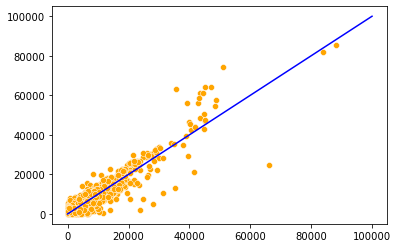
\includegraphics[keepaspectratio]{bagging_files/figure-pdf/cell-14-output-2.png}}

\textbf{Quick Takeaway}

\begin{itemize}
\tightlist
\item
  \textbf{OOB estimates become more reliable} as the number of trees
  grows, with OOB scores closely tracking the test performance after
  around 30 estimators.
\item
  \textbf{OOB RMSE is consistently higher} and \textbf{OOB R² is
  consistently lower} than their test counterparts when the ensemble is
  small, highlighting the \textbf{instability of OOB estimates with few
  trees}.
\end{itemize}

\begin{Shaded}
\begin{Highlighting}[]
\CommentTok{\# get the number of estimators that gives the best OOB RMSE score}
\NormalTok{best\_oob\_rmse\_index }\OperatorTok{=}\NormalTok{ np.argmin(oob\_rmse\_scores)}
\NormalTok{best\_oob\_rmse\_n\_estimators }\OperatorTok{=}\NormalTok{ n\_estimators[best\_oob\_rmse\_index]}
\NormalTok{best\_oob\_rmse\_value }\OperatorTok{=}\NormalTok{ oob\_rmse\_scores[best\_oob\_rmse\_index]}
\BuiltInTok{print}\NormalTok{(}\StringTok{"Best number of estimators for OOB RMSE:"}\NormalTok{, best\_oob\_rmse\_n\_estimators)}
\BuiltInTok{print}\NormalTok{(}\StringTok{"Best OOB RMSE value:"}\NormalTok{, }\BuiltInTok{round}\NormalTok{(best\_oob\_rmse\_value, }\DecValTok{2}\NormalTok{))}
\end{Highlighting}
\end{Shaded}

\begin{verbatim}
Best number of estimators for OOB RMSE: 30
Best OOB RMSE value: 3539.1
\end{verbatim}

\section{Bagging Hyperparameter
Tuning}\label{bagging-hyperparameter-tuning}

To further improve the performance of our bagging model, we can tune key
hyperparameters such as:

\begin{itemize}
\tightlist
\item
  \texttt{n\_estimators}: the number of base estimators in the ensemble,
\item
  \texttt{max\_features}: the maximum number of features considered at
  each split,
\item
  \texttt{max\_samples}: the size of each bootstrap sample used to train
  base estimators,
\item
  \texttt{bootstrap}: whether sampling is performed with replacement
  (\texttt{True}) or without (\texttt{False}),
\item
  \texttt{bootstrap\_features}: whether features are sampled with
  replacement when selecting subsets of features for each estimator.
\end{itemize}

By systematically exploring different combinations of these parameters,
we aim to identify the optimal settings that enhance predictive accuracy
while maintaining good generalization.

There are two common approaches for tuning these hyperparameters: -
\textbf{Cross-validation}, which provides a robust estimate of model
performance, and\\
- \textbf{Out-of-Bag (OOB) score}, which offers an efficient built-in
alternative without needing a separate validation set.

\subsection{Tuning with
Cross-Validation}\label{tuning-with-cross-validation}

Next, let's use \texttt{GridSearchCV} to tune these hyperparameters and
identify the best combination for improved model performance.

\begin{Shaded}
\begin{Highlighting}[]
\CommentTok{\# hyperparameter tuning using GridSearchCV}
\NormalTok{param\_grid }\OperatorTok{=}\NormalTok{ \{}
    \StringTok{\textquotesingle{}n\_estimators\textquotesingle{}}\NormalTok{: [}\DecValTok{10}\NormalTok{, }\DecValTok{20}\NormalTok{, }\DecValTok{30}\NormalTok{, }\DecValTok{40}\NormalTok{, }\DecValTok{50}\NormalTok{],}
    \StringTok{\textquotesingle{}max\_samples\textquotesingle{}}\NormalTok{: [}\FloatTok{0.5}\NormalTok{, }\FloatTok{0.75}\NormalTok{, }\FloatTok{1.0}\NormalTok{],}
    \StringTok{\textquotesingle{}max\_features\textquotesingle{}}\NormalTok{: [}\FloatTok{0.5}\NormalTok{, }\FloatTok{0.75}\NormalTok{, }\FloatTok{1.0}\NormalTok{],}
    \StringTok{\textquotesingle{}bootstrap\textquotesingle{}}\NormalTok{: [}\VariableTok{True}\NormalTok{, }\VariableTok{False}\NormalTok{],}
    \StringTok{\textquotesingle{}bootstrap\_features\textquotesingle{}}\NormalTok{: [}\VariableTok{True}\NormalTok{, }\VariableTok{False}\NormalTok{]}
\NormalTok{\}}

\NormalTok{bagging\_reg\_grid }\OperatorTok{=}\NormalTok{ BaggingRegressor(random\_state}\OperatorTok{=}\DecValTok{42}\NormalTok{, n\_jobs}\OperatorTok{={-}}\DecValTok{1}\NormalTok{)}
\NormalTok{grid\_search }\OperatorTok{=}\NormalTok{ GridSearchCV(bagging\_reg\_grid, param\_grid, cv}\OperatorTok{=}\DecValTok{5}\NormalTok{, scoring}\OperatorTok{=}\StringTok{\textquotesingle{}neg\_mean\_squared\_error\textquotesingle{}}\NormalTok{, n\_jobs}\OperatorTok{={-}}\DecValTok{1}\NormalTok{)}
\NormalTok{grid\_search.fit(X\_train\_final, y\_train)}

\CommentTok{\# get the best parameters and the best score}
\NormalTok{best\_params }\OperatorTok{=}\NormalTok{ grid\_search.best\_params\_}
\NormalTok{best\_score }\OperatorTok{=}\NormalTok{ np.sqrt(}\OperatorTok{{-}}\NormalTok{grid\_search.best\_score\_)}
\BuiltInTok{print}\NormalTok{(}\StringTok{"Best parameters:"}\NormalTok{, best\_params)}
\BuiltInTok{print}\NormalTok{(}\StringTok{"Best RMSE cv score:"}\NormalTok{, }\BuiltInTok{round}\NormalTok{(best\_score, }\DecValTok{2}\NormalTok{))}

\CommentTok{\# make predictions on the test set using the best parameters}
\NormalTok{best\_bagging\_reg }\OperatorTok{=}\NormalTok{ grid\_search.best\_estimator\_}
\NormalTok{y\_pred\_best\_bagging }\OperatorTok{=}\NormalTok{ best\_bagging\_reg.predict(X\_test\_final)}

\CommentTok{\# calculate the RMSE and R\^{}2 score}
\NormalTok{rmse\_best\_bagging }\OperatorTok{=}\NormalTok{ root\_mean\_squared\_error(y\_test, y\_pred\_best\_bagging)}
\NormalTok{r2\_best\_bagging }\OperatorTok{=}\NormalTok{ r2\_score(y\_test, y\_pred\_best\_bagging)}
\BuiltInTok{print}\NormalTok{(}\StringTok{"Test RMSE with best Bagging model:"}\NormalTok{, }\BuiltInTok{round}\NormalTok{(rmse\_best\_bagging, }\DecValTok{2}\NormalTok{))}
\BuiltInTok{print}\NormalTok{(}\StringTok{"Test R\^{}2 score with best Bagging model:"}\NormalTok{, }\BuiltInTok{round}\NormalTok{(r2\_best\_bagging, }\DecValTok{2}\NormalTok{))}

\CommentTok{\# training RMSE and R\^{}2 score}
\NormalTok{y\_pred\_train\_best\_bagging }\OperatorTok{=}\NormalTok{ best\_bagging\_reg.predict(X\_train\_final)}

\CommentTok{\# calculate the RMSE and R\^{}2 score}
\NormalTok{rmse\_train\_best\_bagging }\OperatorTok{=}\NormalTok{ root\_mean\_squared\_error(y\_train, y\_pred\_train\_best\_bagging)}
\NormalTok{r2\_train\_best\_bagging }\OperatorTok{=}\NormalTok{ r2\_score(y\_train, y\_pred\_train\_best\_bagging)}
\BuiltInTok{print}\NormalTok{(}\StringTok{"Train RMSE with best Bagging model:"}\NormalTok{, }\BuiltInTok{round}\NormalTok{(rmse\_train\_best\_bagging, }\DecValTok{2}\NormalTok{))}
\BuiltInTok{print}\NormalTok{(}\StringTok{"Train R\^{}2 score with best Bagging model:"}\NormalTok{, }\BuiltInTok{round}\NormalTok{(r2\_train\_best\_bagging, }\DecValTok{2}\NormalTok{))}
\end{Highlighting}
\end{Shaded}

\begin{verbatim}
Best parameters: {'bootstrap': True, 'bootstrap_features': False, 'max_features': 0.75, 'max_samples': 1.0, 'n_estimators': 50}
Best RMSE cv score: 3288.03
Test RMSE with best Bagging model: 3348.45
Test R^2 score with best Bagging model: 0.96
Train RMSE with best Bagging model: 1411.13
Train R^2 score with best Bagging model: 0.99
\end{verbatim}

After simultaneously tuning multiple hyperparameters of the bagging
model, including \texttt{n\_estimators}, \texttt{max\_features}, and
\texttt{max\_samples}, we achieved the best performance:

\begin{itemize}
\tightlist
\item
  \textbf{Test RMSE with best Bagging model:} 3348.45\\
\item
  \textbf{Test R² score with best Bagging model:} 0.96
\end{itemize}

This demonstrates that careful tuning of bagging-specific parameters can
lead to further improvements beyond using default or even optimized
single decision trees.

\subsection{Tuning with Out-of-Bag (OOB)
Score}\label{tuning-with-out-of-bag-oob-score}

As an alternative to cross-validation, we can use the \textbf{Out-of-Bag
(OOB) score} to evaluate model performance during training.\\
This method is more efficient for large datasets, as it avoids the need
to split data or run multiple folds.

By enabling \texttt{oob\_score=True}, we can monitor performance on
unseen data points (those not included in each bootstrap sample) and use
this score to guide hyperparameter tuning.

\begin{Shaded}
\begin{Highlighting}[]
\ImportTok{from}\NormalTok{ sklearn.model\_selection }\ImportTok{import}\NormalTok{ ParameterGrid}
\CommentTok{\# tune the hyperparameters of the decision tree regressor using oob score}
\CommentTok{\# Hyperparameter grid}
\NormalTok{param\_grid }\OperatorTok{=}\NormalTok{ \{}
    \StringTok{\textquotesingle{}n\_estimators\textquotesingle{}}\NormalTok{: [}\DecValTok{10}\NormalTok{, }\DecValTok{20}\NormalTok{, }\DecValTok{30}\NormalTok{, }\DecValTok{40}\NormalTok{, }\DecValTok{50}\NormalTok{],}
    \StringTok{\textquotesingle{}max\_samples\textquotesingle{}}\NormalTok{: [}\FloatTok{0.5}\NormalTok{, }\FloatTok{0.75}\NormalTok{, }\FloatTok{1.0}\NormalTok{],}
    \StringTok{\textquotesingle{}max\_features\textquotesingle{}}\NormalTok{: [}\FloatTok{0.5}\NormalTok{, }\FloatTok{0.75}\NormalTok{, }\FloatTok{1.0}\NormalTok{],}
    \StringTok{\textquotesingle{}bootstrap\textquotesingle{}}\NormalTok{: [}\VariableTok{True}\NormalTok{],  }\CommentTok{\# Required for OOB}
    \StringTok{\textquotesingle{}bootstrap\_features\textquotesingle{}}\NormalTok{: [}\VariableTok{True}\NormalTok{, }\VariableTok{False}\NormalTok{]}
\NormalTok{\}}

\CommentTok{\# Track best parameters and OOB score}
\NormalTok{best\_score }\OperatorTok{=} \OperatorTok{{-}}\NormalTok{np.inf}
\NormalTok{best\_params }\OperatorTok{=}\NormalTok{ \{\}}

\CommentTok{\# Iterate over all hyperparameter combinations}
\ControlFlowTok{for}\NormalTok{ params }\KeywordTok{in}\NormalTok{ ParameterGrid(param\_grid):}
    \CommentTok{\# Train model with current params and OOB score enabled}
\NormalTok{    model }\OperatorTok{=}\NormalTok{ BaggingRegressor(}
\NormalTok{        estimator}\OperatorTok{=}\NormalTok{tree\_reg,}
        \OperatorTok{**}\NormalTok{params,}
\NormalTok{        oob\_score}\OperatorTok{=}\VariableTok{True}\NormalTok{,}
\NormalTok{        random\_state}\OperatorTok{=}\DecValTok{42}\NormalTok{,}
\NormalTok{        n\_jobs}\OperatorTok{={-}}\DecValTok{1}
\NormalTok{    )}
\NormalTok{    model.fit(X\_train\_final, y\_train)}
    
    \CommentTok{\# Get OOB score (higher is better for R², lower for RMSE)}
\NormalTok{    current\_score }\OperatorTok{=}\NormalTok{ model.oob\_score\_}
    
    \CommentTok{\# Update best params if current score is better}
    \ControlFlowTok{if}\NormalTok{ current\_score }\OperatorTok{\textgreater{}}\NormalTok{ best\_score:}
\NormalTok{        best\_score }\OperatorTok{=}\NormalTok{ current\_score}
\NormalTok{        best\_params }\OperatorTok{=}\NormalTok{ params}

\CommentTok{\# Best model}
\NormalTok{best\_model }\OperatorTok{=}\NormalTok{ BaggingRegressor(}
\NormalTok{    estimator}\OperatorTok{=}\NormalTok{tree\_reg,}
    \OperatorTok{**}\NormalTok{best\_params,}
\NormalTok{    oob\_score}\OperatorTok{=}\VariableTok{True}\NormalTok{,}
\NormalTok{    random\_state}\OperatorTok{=}\DecValTok{42}\NormalTok{,}
\NormalTok{    n\_jobs}\OperatorTok{={-}}\DecValTok{1}
\NormalTok{)}
\NormalTok{best\_model.fit(X\_train\_final, y\_train)}

\BuiltInTok{print}\NormalTok{(}\StringTok{"Best Hyperparameters:"}\NormalTok{, best\_params)}
\BuiltInTok{print}\NormalTok{(}\StringTok{"Best OOB Score:"}\NormalTok{, best\_score)}
\end{Highlighting}
\end{Shaded}

\begin{verbatim}
c:\Users\lsi8012\AppData\Local\anaconda3\Lib\site-packages\sklearn\ensemble\_bagging.py:1315: UserWarning: Some inputs do not have OOB scores. This probably means too few estimators were used to compute any reliable oob estimates.
  warn(
c:\Users\lsi8012\AppData\Local\anaconda3\Lib\site-packages\sklearn\ensemble\_bagging.py:1315: UserWarning: Some inputs do not have OOB scores. This probably means too few estimators were used to compute any reliable oob estimates.
  warn(
c:\Users\lsi8012\AppData\Local\anaconda3\Lib\site-packages\sklearn\ensemble\_bagging.py:1315: UserWarning: Some inputs do not have OOB scores. This probably means too few estimators were used to compute any reliable oob estimates.
  warn(
c:\Users\lsi8012\AppData\Local\anaconda3\Lib\site-packages\sklearn\ensemble\_bagging.py:1315: UserWarning: Some inputs do not have OOB scores. This probably means too few estimators were used to compute any reliable oob estimates.
  warn(
c:\Users\lsi8012\AppData\Local\anaconda3\Lib\site-packages\sklearn\ensemble\_bagging.py:1315: UserWarning: Some inputs do not have OOB scores. This probably means too few estimators were used to compute any reliable oob estimates.
  warn(
c:\Users\lsi8012\AppData\Local\anaconda3\Lib\site-packages\sklearn\ensemble\_bagging.py:1315: UserWarning: Some inputs do not have OOB scores. This probably means too few estimators were used to compute any reliable oob estimates.
  warn(
c:\Users\lsi8012\AppData\Local\anaconda3\Lib\site-packages\sklearn\ensemble\_bagging.py:1315: UserWarning: Some inputs do not have OOB scores. This probably means too few estimators were used to compute any reliable oob estimates.
  warn(
c:\Users\lsi8012\AppData\Local\anaconda3\Lib\site-packages\sklearn\ensemble\_bagging.py:1315: UserWarning: Some inputs do not have OOB scores. This probably means too few estimators were used to compute any reliable oob estimates.
  warn(
c:\Users\lsi8012\AppData\Local\anaconda3\Lib\site-packages\sklearn\ensemble\_bagging.py:1315: UserWarning: Some inputs do not have OOB scores. This probably means too few estimators were used to compute any reliable oob estimates.
  warn(
c:\Users\lsi8012\AppData\Local\anaconda3\Lib\site-packages\sklearn\ensemble\_bagging.py:1315: UserWarning: Some inputs do not have OOB scores. This probably means too few estimators were used to compute any reliable oob estimates.
  warn(
c:\Users\lsi8012\AppData\Local\anaconda3\Lib\site-packages\sklearn\ensemble\_bagging.py:1315: UserWarning: Some inputs do not have OOB scores. This probably means too few estimators were used to compute any reliable oob estimates.
  warn(
c:\Users\lsi8012\AppData\Local\anaconda3\Lib\site-packages\sklearn\ensemble\_bagging.py:1315: UserWarning: Some inputs do not have OOB scores. This probably means too few estimators were used to compute any reliable oob estimates.
  warn(
c:\Users\lsi8012\AppData\Local\anaconda3\Lib\site-packages\sklearn\ensemble\_bagging.py:1315: UserWarning: Some inputs do not have OOB scores. This probably means too few estimators were used to compute any reliable oob estimates.
  warn(
c:\Users\lsi8012\AppData\Local\anaconda3\Lib\site-packages\sklearn\ensemble\_bagging.py:1315: UserWarning: Some inputs do not have OOB scores. This probably means too few estimators were used to compute any reliable oob estimates.
  warn(
c:\Users\lsi8012\AppData\Local\anaconda3\Lib\site-packages\sklearn\ensemble\_bagging.py:1315: UserWarning: Some inputs do not have OOB scores. This probably means too few estimators were used to compute any reliable oob estimates.
  warn(
c:\Users\lsi8012\AppData\Local\anaconda3\Lib\site-packages\sklearn\ensemble\_bagging.py:1315: UserWarning: Some inputs do not have OOB scores. This probably means too few estimators were used to compute any reliable oob estimates.
  warn(
c:\Users\lsi8012\AppData\Local\anaconda3\Lib\site-packages\sklearn\ensemble\_bagging.py:1315: UserWarning: Some inputs do not have OOB scores. This probably means too few estimators were used to compute any reliable oob estimates.
  warn(
c:\Users\lsi8012\AppData\Local\anaconda3\Lib\site-packages\sklearn\ensemble\_bagging.py:1315: UserWarning: Some inputs do not have OOB scores. This probably means too few estimators were used to compute any reliable oob estimates.
  warn(
\end{verbatim}

\begin{verbatim}
Best Hyperparameters: {'bootstrap': True, 'bootstrap_features': False, 'max_features': 0.75, 'max_samples': 0.75, 'n_estimators': 50}
Best OOB Score: 0.9587800605892783
\end{verbatim}

\begin{Shaded}
\begin{Highlighting}[]
\CommentTok{\# output the test RMSE and R\^{}2 score with the best model}
\NormalTok{y\_pred\_best\_model }\OperatorTok{=}\NormalTok{ best\_model.predict(X\_test\_final)}
\NormalTok{rmse\_best\_model }\OperatorTok{=}\NormalTok{ root\_mean\_squared\_error(y\_test, y\_pred\_best\_model)}
\NormalTok{r2\_best\_model }\OperatorTok{=}\NormalTok{ r2\_score(y\_test, y\_pred\_best\_model)}
\BuiltInTok{print}\NormalTok{(}\StringTok{"Test RMSE with best model:"}\NormalTok{, }\BuiltInTok{round}\NormalTok{(rmse\_best\_model, }\DecValTok{2}\NormalTok{))}
\BuiltInTok{print}\NormalTok{(}\StringTok{"Test R\^{}2 score with best model:"}\NormalTok{, }\BuiltInTok{round}\NormalTok{(r2\_best\_model, }\DecValTok{2}\NormalTok{))}
\end{Highlighting}
\end{Shaded}

\begin{verbatim}
Test RMSE with best model: 3418.55
Test R^2 score with best model: 0.96
\end{verbatim}

\subsection{Comparing Hyperparameter Tuning: Cross-Validation vs.~OOB
Score}\label{comparing-hyperparameter-tuning-cross-validation-vs.-oob-score}

\begin{longtable}[]{@{}
  >{\raggedright\arraybackslash}p{(\linewidth - 4\tabcolsep) * \real{0.2044}}
  >{\raggedright\arraybackslash}p{(\linewidth - 4\tabcolsep) * \real{0.4015}}
  >{\raggedright\arraybackslash}p{(\linewidth - 4\tabcolsep) * \real{0.3942}}@{}}
\toprule\noalign{}
\begin{minipage}[b]{\linewidth}\raggedright
Aspect
\end{minipage} & \begin{minipage}[b]{\linewidth}\raggedright
Cross-Validation (CV)
\end{minipage} & \begin{minipage}[b]{\linewidth}\raggedright
Out-of-Bag (OOB) Score
\end{minipage} \\
\midrule\noalign{}
\endhead
\bottomrule\noalign{}
\endlastfoot
\textbf{Mechanism} & Splits training data into multiple folds to
validate & Uses unused (out-of-bag) samples in each bootstrap \\
\textbf{Requires Manual Splits?} & Yes & No --- internal to bagging
process \\
\textbf{Efficiency} & Slower, especially for large datasets & Faster and
more efficient for large datasets \\
\textbf{Bias-Variance Tradeoff} & More stable and less biased
performance estimate & Slightly more variable and can underestimate
accuracy \\
\textbf{Availability} & Available for all models & Only available when
\texttt{bootstrap=True} in bagging \\
\textbf{Integration in Sklearn} & Built-in via \texttt{GridSearchCV} &
Must be implemented manually for tuning \\
\textbf{Flexibility} & Works with any model type & Only works with
bagging-based models \\
\textbf{Use Case} & Ideal for robust model comparison & Great for quick
tuning on large datasets \\
\textbf{Scoring Access} & \texttt{.best\_score\_} from
\texttt{GridSearchCV} & \texttt{.oob\_score\_} from trained model \\
\end{longtable}

\subsubsection{✅ Best Practices for Imbalanced
Classification}\label{best-practices-for-imbalanced-classification}

\begin{itemize}
\tightlist
\item
  \textbf{Prefer Cross-Validation}, especially with:

  \begin{itemize}
  \tightlist
  \item
    \texttt{StratifiedKFold} to maintain class distribution in each
    fold.
  \item
    Custom metrics (e.g., F1-score, ROC-AUC, balanced accuracy) using
    \texttt{scoring=}.
  \end{itemize}
\item
  \textbf{Be cautious using OOB score:}

  \begin{itemize}
  \tightlist
  \item
    OOB score may be misleading for \textbf{rare classes}, especially
    when \texttt{n\_estimators} is small.
  \item
    Only use it for \textbf{rough estimates} or \textbf{early tuning}
    when computational efficiency is critical.
  \end{itemize}
\end{itemize}

\#\#\#\# ✅ Summary

\begin{itemize}
\tightlist
\item
  \textbf{Use Cross-Validation} when:

  \begin{itemize}
  \tightlist
  \item
    You want robust, model-agnostic performance evaluation.
  \item
    You need precise comparisons between different model types or
    pipelines.
  \item
    You work on imbalanced classification task
  \end{itemize}
\item
  \textbf{Use OOB Score} when:

  \begin{itemize}
  \tightlist
  \item
    You're working with large datasets and want faster tuning.
  \item
    Your model is based on bagging (e.g., \texttt{BaggingClassifier},
    \texttt{RandomForestClassifier}).
  \item
    You want to avoid manual train/validation splits.
  \end{itemize}
\end{itemize}

\begin{quote}
⚠️ Note: Scikit-learn's \texttt{GridSearchCV} \textbf{does not use OOB
score} for tuning---even if \texttt{oob\_score=True} is set. To use OOB
for tuning, you must loop over hyperparameters manually and evaluate
using \texttt{.oob\_score\_}.
\end{quote}

\section{Bagging Classification
Trees}\label{bagging-classification-trees}

Let's revisit the same dataset used for building a single classification
tree.\\
When using the default settings, the tree tends to \textbf{overfit} the
data, as shown
\href{https://lizhen0909.github.io/STAT303-3-class-notes/Classification\%20_Tree.html\#building-a-classification-tree}{here}.

In that notebook, we addressed the overfitting issue using both
\textbf{pre-pruning} and \textbf{post-pruning} techniques.\\
Now, we'll explore an alternative approach---\textbf{bagging}---to
reduce overfitting and improve model performance.

\begin{Shaded}
\begin{Highlighting}[]
\CommentTok{\# load the dataset}
\NormalTok{heart\_df  }\OperatorTok{=}\NormalTok{ pd.read\_csv(}\StringTok{\textquotesingle{}datasets/heart\_disease\_classification.csv\textquotesingle{}}\NormalTok{)}
\BuiltInTok{print}\NormalTok{(heart\_df .shape)}
\NormalTok{heart\_df .head()}
\end{Highlighting}
\end{Shaded}

\begin{verbatim}
(303, 14)
\end{verbatim}

\begin{longtable}[]{@{}lllllllllllllll@{}}
\toprule\noalign{}
& age & sex & cp & trestbps & chol & fbs & restecg & thalach & exang &
oldpeak & slope & ca & thal & target \\
\midrule\noalign{}
\endhead
\bottomrule\noalign{}
\endlastfoot
0 & 63 & 1 & 3 & 145 & 233 & 1 & 0 & 150 & 0 & 2.3 & 0 & 0 & 1 & 1 \\
1 & 37 & 1 & 2 & 130 & 250 & 0 & 1 & 187 & 0 & 3.5 & 0 & 0 & 2 & 1 \\
2 & 41 & 0 & 1 & 130 & 204 & 0 & 0 & 172 & 0 & 1.4 & 2 & 0 & 2 & 1 \\
3 & 56 & 1 & 1 & 120 & 236 & 0 & 1 & 178 & 0 & 0.8 & 2 & 0 & 2 & 1 \\
4 & 57 & 0 & 0 & 120 & 354 & 0 & 1 & 163 & 1 & 0.6 & 2 & 0 & 2 & 1 \\
\end{longtable}

\begin{Shaded}
\begin{Highlighting}[]
\CommentTok{\# split the x and y data}
\NormalTok{X\_cls }\OperatorTok{=}\NormalTok{ heart\_df.drop(columns}\OperatorTok{=}\NormalTok{[}\StringTok{\textquotesingle{}target\textquotesingle{}}\NormalTok{])}
\NormalTok{y\_cls }\OperatorTok{=}\NormalTok{ heart\_df.target}

\CommentTok{\# split the data into train and test sets, add \_cls to the variable names}
\NormalTok{X\_train\_cls, X\_test\_cls, y\_train\_cls, y\_test\_cls }\OperatorTok{=}\NormalTok{ train\_test\_split(X\_cls, y\_cls, test\_size}\OperatorTok{=}\FloatTok{0.2}\NormalTok{, random\_state}\OperatorTok{=}\DecValTok{42}\NormalTok{)}
\end{Highlighting}
\end{Shaded}

\begin{Shaded}
\begin{Highlighting}[]
\CommentTok{\# using tree bagging to fit the data}

\NormalTok{bagging }\OperatorTok{=}\NormalTok{ BaggingClassifier(DecisionTreeClassifier(), n\_estimators}\OperatorTok{=}\DecValTok{100}\NormalTok{, random\_state}\OperatorTok{=}\DecValTok{0}\NormalTok{)}
\NormalTok{bagging.fit(X\_train\_cls, y\_train\_cls)}

\NormalTok{y\_pred\_train\_cls }\OperatorTok{=}\NormalTok{ bagging.predict(X\_train\_cls)}
\NormalTok{y\_pred\_cls }\OperatorTok{=}\NormalTok{ bagging.predict(X\_test\_cls)}


\CommentTok{\#print out the accuracy on test set and training set}
\BuiltInTok{print}\NormalTok{(}\StringTok{"Train Accuracy is "}\NormalTok{, accuracy\_score(y\_train\_cls,y\_pred\_train\_cls)}\OperatorTok{*}\DecValTok{100}\NormalTok{)}
\BuiltInTok{print}\NormalTok{(}\StringTok{"Test Accuracy is "}\NormalTok{, accuracy\_score(y\_test\_cls,y\_pred\_cls)}\OperatorTok{*}\DecValTok{100}\NormalTok{)}
\end{Highlighting}
\end{Shaded}

\begin{verbatim}
Train Accuracy is  100.0
Test Accuracy is  85.24590163934425
\end{verbatim}

\chapter{Random Forests}\label{random-forests}

\emph{Read section 8.2.2 of the book before using these notes.}

\emph{Note that in this course, lecture notes are not sufficient, you
must read the book for better understanding. Lecture notes are just
implementing the concepts of the book on a dataset, but not explaining
the concepts elaborately.}

\begin{Shaded}
\begin{Highlighting}[]
\CommentTok{\# Importing necessary libraries}
\ImportTok{import}\NormalTok{ pandas }\ImportTok{as}\NormalTok{ pd}
\ImportTok{import}\NormalTok{ numpy }\ImportTok{as}\NormalTok{ np}
\ImportTok{import}\NormalTok{ matplotlib.pyplot }\ImportTok{as}\NormalTok{ plt}
\ImportTok{import}\NormalTok{ seaborn }\ImportTok{as}\NormalTok{ sns}
\NormalTok{sns.}\BuiltInTok{set}\NormalTok{(font\_scale}\OperatorTok{=}\FloatTok{1.35}\NormalTok{)}

\CommentTok{\# import the decision tree regressor}
\ImportTok{from}\NormalTok{ sklearn.tree }\ImportTok{import}\NormalTok{ DecisionTreeRegressor, DecisionTreeClassifier, plot\_tree, export\_graphviz}
\ImportTok{from}\NormalTok{ sklearn.ensemble }\ImportTok{import}\NormalTok{ BaggingRegressor,BaggingClassifier}

\CommentTok{\# split the dataset into training and testing sets}
\ImportTok{from}\NormalTok{ sklearn.model\_selection }\ImportTok{import}\NormalTok{ train\_test\_split}


\ImportTok{from}\NormalTok{ sklearn.model\_selection }\ImportTok{import}\NormalTok{ cross\_val\_score, GridSearchCV, cross\_val\_predict, KFold}

\ImportTok{from}\NormalTok{ sklearn.pipeline }\ImportTok{import}\NormalTok{ Pipeline}
\ImportTok{from}\NormalTok{ sklearn.compose }\ImportTok{import}\NormalTok{ ColumnTransformer}
\ImportTok{from}\NormalTok{ sklearn.preprocessing }\ImportTok{import}\NormalTok{ OneHotEncoder, FunctionTransformer}
\ImportTok{from}\NormalTok{ sklearn.metrics }\ImportTok{import}\NormalTok{ root\_mean\_squared\_error, r2\_score, make\_scorer, accuracy\_score}
\end{Highlighting}
\end{Shaded}

\section{Motivation: Bagging
Revisited}\label{motivation-bagging-revisited}

In Bagging (Bootstrap Aggregating), we:

\begin{itemize}
\item
  Train many trees on different bootstrap samples of the training data.
\item
  Aggregate their predictions by averaging (regression) or voting
  (classification).
\end{itemize}

\begin{quote}
✅ Bagging helps reduce variance ⚠️ But if the trees are too similar
(i.e., highly correlated), averaging won't help as much.
\end{quote}

\begin{Shaded}
\begin{Highlighting}[]
\CommentTok{\# Load the dataset}
\NormalTok{car }\OperatorTok{=}\NormalTok{ pd.read\_csv(}\StringTok{\textquotesingle{}Datasets/car.csv\textquotesingle{}}\NormalTok{)}
\NormalTok{car.head()}
\end{Highlighting}
\end{Shaded}

\begin{longtable}[]{@{}lllllllllll@{}}
\toprule\noalign{}
& brand & model & year & transmission & mileage & fuelType & tax & mpg &
engineSize & price \\
\midrule\noalign{}
\endhead
\bottomrule\noalign{}
\endlastfoot
0 & vw & Beetle & 2014 & Manual & 55457 & Diesel & 30 & 65.3266 & 1.6 &
7490 \\
1 & vauxhall & GTC & 2017 & Manual & 15630 & Petrol & 145 & 47.2049 &
1.4 & 10998 \\
2 & merc & G Class & 2012 & Automatic & 43000 & Diesel & 570 & 25.1172 &
3.0 & 44990 \\
3 & audi & RS5 & 2019 & Automatic & 10 & Petrol & 145 & 30.5593 & 2.9 &
51990 \\
4 & merc & X-CLASS & 2018 & Automatic & 14000 & Diesel & 240 & 35.7168 &
2.3 & 28990 \\
\end{longtable}

\begin{Shaded}
\begin{Highlighting}[]
\NormalTok{X }\OperatorTok{=}\NormalTok{ car.drop(columns}\OperatorTok{=}\NormalTok{[}\StringTok{\textquotesingle{}price\textquotesingle{}}\NormalTok{])}
\NormalTok{y }\OperatorTok{=}\NormalTok{ car[}\StringTok{\textquotesingle{}price\textquotesingle{}}\NormalTok{]}

\NormalTok{X\_train, X\_test, y\_train, y\_test }\OperatorTok{=}\NormalTok{ train\_test\_split(X, y, test\_size}\OperatorTok{=}\FloatTok{0.2}\NormalTok{, random\_state}\OperatorTok{=}\DecValTok{42}\NormalTok{)}

\CommentTok{\# extract the categorical columns and put them in a list}
\NormalTok{categorical\_feature }\OperatorTok{=}\NormalTok{ X.select\_dtypes(include}\OperatorTok{=}\NormalTok{[}\StringTok{\textquotesingle{}object\textquotesingle{}}\NormalTok{]).columns.tolist()}

\CommentTok{\# extract the numerical columns and put them in a list}
\NormalTok{numerical\_feature }\OperatorTok{=}\NormalTok{ X.select\_dtypes(include}\OperatorTok{=}\NormalTok{[}\StringTok{\textquotesingle{}int64\textquotesingle{}}\NormalTok{, }\StringTok{\textquotesingle{}float64\textquotesingle{}}\NormalTok{]).columns.tolist()}
\end{Highlighting}
\end{Shaded}

\begin{Shaded}
\begin{Highlighting}[]
\NormalTok{preprocessor }\OperatorTok{=}\NormalTok{ ColumnTransformer(}
\NormalTok{    transformers}\OperatorTok{=}\NormalTok{[}
\NormalTok{        (}\StringTok{\textquotesingle{}num\textquotesingle{}}\NormalTok{, FunctionTransformer(), numerical\_feature),}
\NormalTok{        (}\StringTok{\textquotesingle{}cat\textquotesingle{}}\NormalTok{, OneHotEncoder(handle\_unknown}\OperatorTok{=}\StringTok{\textquotesingle{}ignore\textquotesingle{}}\NormalTok{), categorical\_feature)}
\NormalTok{    ],}
\NormalTok{    remainder}\OperatorTok{=}\StringTok{\textquotesingle{}passthrough\textquotesingle{}}
\NormalTok{)}
\end{Highlighting}
\end{Shaded}

\subsection{Let's build a single decision tree and output its
performance}\label{lets-build-a-single-decision-tree-and-output-its-performance}

\begin{Shaded}
\begin{Highlighting}[]
\CommentTok{\# build a single decsision tree regressor}
\NormalTok{single\_tree\_regressor }\OperatorTok{=}\NormalTok{ DecisionTreeRegressor(random\_state}\OperatorTok{=}\DecValTok{0}\NormalTok{)}

\CommentTok{\# pipeline for the single decision tree regressor}
\NormalTok{single\_tree\_pipeline }\OperatorTok{=}\NormalTok{ Pipeline(steps}\OperatorTok{=}\NormalTok{[}
\NormalTok{    (}\StringTok{\textquotesingle{}preprocessor\textquotesingle{}}\NormalTok{, preprocessor),}
\NormalTok{    (}\StringTok{\textquotesingle{}tree\textquotesingle{}}\NormalTok{, single\_tree\_regressor)}
\NormalTok{])}
\CommentTok{\# fit the pipeline to the training data}
\NormalTok{single\_tree\_pipeline.fit(X\_train, y\_train)}
\CommentTok{\# make predictions on the test data}
\NormalTok{y\_pred\_single\_tree }\OperatorTok{=}\NormalTok{ single\_tree\_pipeline.predict(X\_test)}
\CommentTok{\# calculate the RMSE and R\^{}2 score}
\NormalTok{rmse\_single\_tree }\OperatorTok{=}\NormalTok{ root\_mean\_squared\_error(y\_test, y\_pred\_single\_tree)}
\NormalTok{r2\_single\_tree }\OperatorTok{=}\NormalTok{ r2\_score(y\_test, y\_pred\_single\_tree)}
\BuiltInTok{print}\NormalTok{(}\SpecialStringTok{f\textquotesingle{}Single Tree RMSE: }\SpecialCharTok{\{}\NormalTok{rmse\_single\_tree}\SpecialCharTok{:.2f\}}\SpecialStringTok{\textquotesingle{}}\NormalTok{)}
\BuiltInTok{print}\NormalTok{(}\SpecialStringTok{f\textquotesingle{}Single Tree R\^{}2: }\SpecialCharTok{\{}\NormalTok{r2\_single\_tree}\SpecialCharTok{:.2f\}}\SpecialStringTok{\textquotesingle{}}\NormalTok{)}

\CommentTok{\# calculate the RMSE and R\^{}2 score for the training data}
\NormalTok{y\_pred\_train\_single\_tree }\OperatorTok{=}\NormalTok{ single\_tree\_pipeline.predict(X\_train)}
\NormalTok{rmse\_train\_single\_tree }\OperatorTok{=}\NormalTok{ root\_mean\_squared\_error(y\_train, y\_pred\_train\_single\_tree)}
\NormalTok{r2\_train\_single\_tree }\OperatorTok{=}\NormalTok{ r2\_score(y\_train, y\_pred\_train\_single\_tree)}
\BuiltInTok{print}\NormalTok{(}\SpecialStringTok{f\textquotesingle{}Single Tree Train RMSE: }\SpecialCharTok{\{}\NormalTok{rmse\_train\_single\_tree}\SpecialCharTok{:.2f\}}\SpecialStringTok{\textquotesingle{}}\NormalTok{)}
\BuiltInTok{print}\NormalTok{(}\SpecialStringTok{f\textquotesingle{}Single Tree Train R\^{}2: }\SpecialCharTok{\{}\NormalTok{r2\_train\_single\_tree}\SpecialCharTok{:.2f\}}\SpecialStringTok{\textquotesingle{}}\NormalTok{)}
\end{Highlighting}
\end{Shaded}

\begin{verbatim}
Single Tree RMSE: 5073.81
Single Tree R^2: 0.91
Single Tree Train RMSE: 0.00
Single Tree Train R^2: 1.00
\end{verbatim}

\begin{Shaded}
\begin{Highlighting}[]
\CommentTok{\# single tree depth}
\NormalTok{tree\_depth }\OperatorTok{=}\NormalTok{ single\_tree\_pipeline.named\_steps[}\StringTok{\textquotesingle{}tree\textquotesingle{}}\NormalTok{].get\_depth()}
\BuiltInTok{print}\NormalTok{(}\SpecialStringTok{f"Depth of the single decision tree: }\SpecialCharTok{\{}\NormalTok{tree\_depth}\SpecialCharTok{\}}\SpecialStringTok{"}\NormalTok{)}
\end{Highlighting}
\end{Shaded}

\begin{verbatim}
Depth of the single decision tree: 34
\end{verbatim}

\subsection{Let's Build a Bagging Tree with Bootstrap Sampling to Reduce
Variance}\label{lets-build-a-bagging-tree-with-bootstrap-sampling-to-reduce-variance}

By default, \texttt{bootstrap=True}, meaning each training set is
created by sampling \textbf{with replacement} from the original dataset.

\begin{Shaded}
\begin{Highlighting}[]
\CommentTok{\# bagging with bootstrap}
\NormalTok{bagging\_with\_bootstrap\_regressor }\OperatorTok{=}\NormalTok{ BaggingRegressor(}
\NormalTok{    estimator}\OperatorTok{=}\NormalTok{DecisionTreeRegressor(random\_state}\OperatorTok{=}\DecValTok{0}\NormalTok{),}
\NormalTok{    n\_estimators}\OperatorTok{=}\DecValTok{50}\NormalTok{,}
\NormalTok{    random\_state}\OperatorTok{=}\DecValTok{42}
\NormalTok{)}

\CommentTok{\# create a pipeline with the preprocessor and the bagging regressor}
\NormalTok{bootstrap\_bagging\_pipeline }\OperatorTok{=}\NormalTok{ Pipeline(steps}\OperatorTok{=}\NormalTok{[}
\NormalTok{    (}\StringTok{\textquotesingle{}preprocessor\textquotesingle{}}\NormalTok{, preprocessor),}
\NormalTok{    (}\StringTok{\textquotesingle{}bagging\textquotesingle{}}\NormalTok{, bagging\_with\_bootstrap\_regressor)}
\NormalTok{])}

\CommentTok{\# fit the pipeline to the training data}
\NormalTok{bootstrap\_bagging\_pipeline.fit(X\_train, y\_train)}
\CommentTok{\# make predictions on the test data}
\NormalTok{y\_pred }\OperatorTok{=}\NormalTok{ bootstrap\_bagging\_pipeline.predict(X\_test)}
\CommentTok{\# calculate the RMSE and R\^{}2 score}
\NormalTok{rmse }\OperatorTok{=}\NormalTok{ root\_mean\_squared\_error(y\_test, y\_pred)}
\NormalTok{r2 }\OperatorTok{=}\NormalTok{ r2\_score(y\_test, y\_pred)}
\BuiltInTok{print}\NormalTok{(}\SpecialStringTok{f\textquotesingle{}RMSE using bootstraping: }\SpecialCharTok{\{}\NormalTok{rmse}\SpecialCharTok{:.2f\}}\SpecialStringTok{\textquotesingle{}}\NormalTok{)}
\BuiltInTok{print}\NormalTok{(}\SpecialStringTok{f\textquotesingle{}R\^{}2 using bootstraping: }\SpecialCharTok{\{}\NormalTok{r2}\SpecialCharTok{:.2f\}}\SpecialStringTok{\textquotesingle{}}\NormalTok{)}
\CommentTok{\# calculate the training rmse and r\^{}2 score}
\NormalTok{y\_train\_pred }\OperatorTok{=}\NormalTok{ bootstrap\_bagging\_pipeline.predict(X\_train)}
\NormalTok{train\_rmse }\OperatorTok{=}\NormalTok{ root\_mean\_squared\_error(y\_train, y\_train\_pred)}
\NormalTok{train\_r2 }\OperatorTok{=}\NormalTok{ r2\_score(y\_train, y\_train\_pred)}
\BuiltInTok{print}\NormalTok{(}\SpecialStringTok{f\textquotesingle{}Training RMSE using bootstraping: }\SpecialCharTok{\{}\NormalTok{train\_rmse}\SpecialCharTok{:.2f\}}\SpecialStringTok{\textquotesingle{}}\NormalTok{)}
\BuiltInTok{print}\NormalTok{(}\SpecialStringTok{f\textquotesingle{}Training R\^{}2 using bootstraping: }\SpecialCharTok{\{}\NormalTok{train\_r2}\SpecialCharTok{:.2f\}}\SpecialStringTok{\textquotesingle{}}\NormalTok{)}
\end{Highlighting}
\end{Shaded}

\begin{verbatim}
RMSE using bootstraping: 3756.85
R^2 using bootstraping: 0.95
Training RMSE using bootstraping: 1395.75
Training R^2 using bootstraping: 0.99
\end{verbatim}

The test RMSE improved significantly from 5073 to 3756, and the R² score
increased from 0.91 to 0.95 after applying bagging.

\subsection{Let's Build a Bagging Tree Without Bootstrap
Sampling}\label{lets-build-a-bagging-tree-without-bootstrap-sampling}

Now, we'll turn off bootstrap sampling (\texttt{bootstrap=False}) and
observe how it affects the bagging model's performance.

\begin{Shaded}
\begin{Highlighting}[]
\NormalTok{bagging\_without\_bootstrap\_regressor }\OperatorTok{=}\NormalTok{ BaggingRegressor(}
\NormalTok{    estimator}\OperatorTok{=}\NormalTok{DecisionTreeRegressor(random\_state}\OperatorTok{=}\DecValTok{0}\NormalTok{),}
\NormalTok{    bootstrap}\OperatorTok{=}\VariableTok{False}\NormalTok{,}
\NormalTok{    n\_estimators}\OperatorTok{=}\DecValTok{50}\NormalTok{,}
\NormalTok{    random\_state}\OperatorTok{=}\DecValTok{42}
\NormalTok{)}

\CommentTok{\# create a pipeline with the preprocessor and the bagging regressor}
\NormalTok{without\_bootstrap\_bagging\_pipeline }\OperatorTok{=}\NormalTok{ Pipeline(steps}\OperatorTok{=}\NormalTok{[}
\NormalTok{    (}\StringTok{\textquotesingle{}preprocessor\textquotesingle{}}\NormalTok{, preprocessor),}
\NormalTok{    (}\StringTok{\textquotesingle{}bagging\textquotesingle{}}\NormalTok{, bagging\_without\_bootstrap\_regressor)}
\NormalTok{])}

\CommentTok{\# fit the pipeline to the training data}
\NormalTok{without\_bootstrap\_bagging\_pipeline.fit(X\_train, y\_train)}
\CommentTok{\# make predictions on the test data}
\NormalTok{y\_pred }\OperatorTok{=}\NormalTok{ without\_bootstrap\_bagging\_pipeline.predict(X\_test)}

\CommentTok{\# calculate the RMSE and R\^{}2 score}
\NormalTok{rmse }\OperatorTok{=}\NormalTok{ root\_mean\_squared\_error(y\_test, y\_pred)}
\NormalTok{r2 }\OperatorTok{=}\NormalTok{ r2\_score(y\_test, y\_pred)}
\BuiltInTok{print}\NormalTok{(}\SpecialStringTok{f\textquotesingle{}RMSE without bootstrap sampling: }\SpecialCharTok{\{}\NormalTok{rmse}\SpecialCharTok{:.2f\}}\SpecialStringTok{\textquotesingle{}}\NormalTok{)}
\BuiltInTok{print}\NormalTok{(}\SpecialStringTok{f\textquotesingle{}R\^{}2 without bootstrap sampling: }\SpecialCharTok{\{}\NormalTok{r2}\SpecialCharTok{:.2f\}}\SpecialStringTok{\textquotesingle{}}\NormalTok{)}

\CommentTok{\# calculate the training rmse and r\^{}2 score}
\NormalTok{y\_train\_pred }\OperatorTok{=}\NormalTok{ without\_bootstrap\_bagging\_pipeline.predict(X\_train)}
\NormalTok{train\_rmse }\OperatorTok{=}\NormalTok{ root\_mean\_squared\_error(y\_train, y\_train\_pred)}
\NormalTok{train\_r2 }\OperatorTok{=}\NormalTok{ r2\_score(y\_train, y\_train\_pred)}
\BuiltInTok{print}\NormalTok{(}\SpecialStringTok{f\textquotesingle{}Training RMSE without bootstrap sampling: }\SpecialCharTok{\{}\NormalTok{train\_rmse}\SpecialCharTok{:.2f\}}\SpecialStringTok{\textquotesingle{}}\NormalTok{)}
\BuiltInTok{print}\NormalTok{(}\SpecialStringTok{f\textquotesingle{}Training R\^{}2 without bootstrap sampling: }\SpecialCharTok{\{}\NormalTok{train\_r2}\SpecialCharTok{:.2f\}}\SpecialStringTok{\textquotesingle{}}\NormalTok{)}
\end{Highlighting}
\end{Shaded}

\begin{verbatim}
RMSE: 4667.43
R^2: 0.93
Training RMSE: 0.00
Training R^2: 1.00
\end{verbatim}

As observed from the results, the performance of bagging without
bootstrap sampling is worse (RMSE: 4667) compared to using bootstrap
sampling (RMSE: 3756).

\subsection{❓ Why Does Bagging Without Bootstrap Perform
Worse?}\label{why-does-bagging-without-bootstrap-perform-worse}

When \texttt{bootstrap=True}, each tree in the ensemble is trained on a
different bootstrap sample --- a random sample drawn \textbf{with
replacement} from the training data. This process has two key effects:

\begin{itemize}
\tightlist
\item
  It \textbf{introduces diversity} among the individual trees.
\item
  It \textbf{reduces correlation} between trees.
\end{itemize}

This diversity is the \textbf{core strength} of bagging: even though
individual trees may overfit, their errors tend to cancel out when their
predictions are averaged, leading to improved generalization.

\subsection{❓ Why Can Bagging Without Bootstrap Still Show Slight
Improvement?}\label{why-can-bagging-without-bootstrap-still-show-slight-improvement}

When \texttt{bootstrap=False}, all trees are trained on the \textbf{same
full dataset}, removing the primary source of diversity in bagging. As a
result, the \textbf{variance reduction benefit} from averaging is
significantly weakened.

However, even when trees are trained on the same data, slight variations
can still arise due to \textbf{internal randomness} in how decision
trees are constructed. For example:

\begin{itemize}
\tightlist
\item
  When multiple splits yield the same information gain, one split may be
  selected \textbf{randomly}.
\item
  \textbf{Ties} between split candidates can be broken differently.
\item
  \textbf{Minor numerical differences} can occur due to floating-point
  operations.
\end{itemize}

These small variations cause the trees to differ slightly, allowing the
ensemble to achieve \textbf{some variance reduction}, which can
\textbf{slightly improve generalization} compared to a single decision
tree.

\begin{quote}
⚠️ However, this improvement is typically \textbf{much smaller} than the
improvement achieved when using full bootstrap sampling
(\texttt{bootstrap=True}).
\end{quote}

\section{Random Forest}\label{random-forest}

While \textbf{diversity} is the core strength of bagging, \textbf{Random
Forest} further improves upon bagging by introducing \textbf{even more
diversity among the individual trees}.

The goal of Random Forest is to \textbf{further decorrelate the trees},
which leads to improved generalization and predictive performance.

\subsection{Idea Behind Random Forest}\label{idea-behind-random-forest}

Random Forest introduces an additional source of randomness:

\begin{itemize}
\tightlist
\item
  At each split in a tree, instead of considering \textbf{all
  predictors}, Random Forest randomly selects a \textbf{subset of
  predictors} to evaluate.
\end{itemize}

This approach:

\begin{itemize}
\tightlist
\item
  Increases \textbf{diversity} among the trees.
\item
  Decreases \textbf{correlation} between trees.
\item
  Further \textbf{reduces the variance} of the aggregated model.
\end{itemize}

\begin{quote}
\textbf{Result}: Random Forest generally achieves better performance
than standard bagging, especially on high-dimensional datasets.
\end{quote}

\subsection{Key Hyperparameter
Comparison}\label{key-hyperparameter-comparison}

\begin{longtable}[]{@{}
  >{\raggedright\arraybackslash}p{(\linewidth - 4\tabcolsep) * \real{0.1720}}
  >{\raggedright\arraybackslash}p{(\linewidth - 4\tabcolsep) * \real{0.3978}}
  >{\raggedright\arraybackslash}p{(\linewidth - 4\tabcolsep) * \real{0.4301}}@{}}
\toprule\noalign{}
\begin{minipage}[b]{\linewidth}\raggedright
Hyperparameter
\end{minipage} & \begin{minipage}[b]{\linewidth}\raggedright
\textbf{Bagging}
\end{minipage} & \begin{minipage}[b]{\linewidth}\raggedright
\textbf{Random Forest}
\end{minipage} \\
\midrule\noalign{}
\endhead
\bottomrule\noalign{}
\endlastfoot
\texttt{bootstrap} & ✅ Yes & ✅ Yes \\
\texttt{max\_features} & 🧩 All features considered at each split & 🧩
Random subset of features at each split \\
\texttt{oob\_score} & ✅ Often used for evaluation & ✅ Often used for
evaluation \\
\texttt{n\_estimators} & ✅ Number of trees & ✅ Number of trees \\
\end{longtable}

\subsection{Let's Build a Random Forest Model Using the Default
Settings}\label{lets-build-a-random-forest-model-using-the-default-settings}

The \texttt{max\_features} hyperparameter controls the number of
features considered when searching for the best split at each node.\\
By default, \texttt{max\_features=1.0}, meaning \textbf{all features}
are considered at every split, similar to standard bagging.

\begin{Shaded}
\begin{Highlighting}[]
\ImportTok{from}\NormalTok{ sklearn.ensemble }\ImportTok{import}\NormalTok{ RandomForestRegressor}

\NormalTok{rf\_regressor }\OperatorTok{=}\NormalTok{ RandomForestRegressor(}
\NormalTok{    n\_estimators}\OperatorTok{=}\DecValTok{50}\NormalTok{,}
\NormalTok{    random\_state}\OperatorTok{=}\DecValTok{42}
\NormalTok{)}

\CommentTok{\# create a pipeline with the preprocessor and the bagging regressor}
\NormalTok{rf\_pipeline }\OperatorTok{=}\NormalTok{ Pipeline(steps}\OperatorTok{=}\NormalTok{[}
\NormalTok{    (}\StringTok{\textquotesingle{}preprocessor\textquotesingle{}}\NormalTok{, preprocessor),}
\NormalTok{    (}\StringTok{\textquotesingle{}rf\textquotesingle{}}\NormalTok{, rf\_regressor)}
\NormalTok{])}

\CommentTok{\# fit the pipeline to the training data}
\NormalTok{rf\_pipeline.fit(X\_train, y\_train)}
\CommentTok{\# make predictions on the test data}
\NormalTok{y\_pred }\OperatorTok{=}\NormalTok{ rf\_pipeline.predict(X\_test)}

\CommentTok{\# calculate the RMSE and R\^{}2 score}
\NormalTok{rmse }\OperatorTok{=}\NormalTok{ root\_mean\_squared\_error(y\_test, y\_pred)}
\NormalTok{r2 }\OperatorTok{=}\NormalTok{ r2\_score(y\_test, y\_pred)}
\BuiltInTok{print}\NormalTok{(}\SpecialStringTok{f\textquotesingle{}RMSE using random forest: }\SpecialCharTok{\{}\NormalTok{rmse}\SpecialCharTok{:.2f\}}\SpecialStringTok{\textquotesingle{}}\NormalTok{)}
\BuiltInTok{print}\NormalTok{(}\SpecialStringTok{f\textquotesingle{}R\^{}2 using random forest: }\SpecialCharTok{\{}\NormalTok{r2}\SpecialCharTok{:.2f\}}\SpecialStringTok{\textquotesingle{}}\NormalTok{)}

\CommentTok{\# calculate the training rmse and r\^{}2 score}
\NormalTok{y\_train\_pred }\OperatorTok{=}\NormalTok{ rf\_pipeline.predict(X\_train)}
\NormalTok{train\_rmse }\OperatorTok{=}\NormalTok{ root\_mean\_squared\_error(y\_train, y\_train\_pred)}
\NormalTok{train\_r2 }\OperatorTok{=}\NormalTok{ r2\_score(y\_train, y\_train\_pred)}
\BuiltInTok{print}\NormalTok{(}\SpecialStringTok{f\textquotesingle{}Training RMSE using random forest: }\SpecialCharTok{\{}\NormalTok{train\_rmse}\SpecialCharTok{:.2f\}}\SpecialStringTok{\textquotesingle{}}\NormalTok{)}
\BuiltInTok{print}\NormalTok{(}\SpecialStringTok{f\textquotesingle{}Training R\^{}2 using random forest: }\SpecialCharTok{\{}\NormalTok{train\_r2}\SpecialCharTok{:.2f\}}\SpecialStringTok{\textquotesingle{}}\NormalTok{)}
\end{Highlighting}
\end{Shaded}

\begin{verbatim}
RMSE: 3747.58
R^2: 0.95
Training RMSE: 1395.03
Training R^2: 0.99
\end{verbatim}

This result is close to that of the bagging model with bootstrap
sampling (RMSE: 3756 vs.~3747).\\
To further decorrelate the trees, we can adjust the
\texttt{max\_features} parameter. Reducing \texttt{max\_features} limits
the number of features considered at each split, which increases
diversity among the trees and helps further reduce variance.

\subsection{\texorpdfstring{Let's Build a Random Forest Model with
\texttt{sqrt}
max\_features}{Let's Build a Random Forest Model with sqrt max\_features}}\label{lets-build-a-random-forest-model-with-sqrt-max_features}

There are two common options to reduce the number of features considered
at each split: \texttt{sqrt} and \texttt{log2}.\\
Here, we will set
\texttt{max\_features=\textquotesingle{}sqrt\textquotesingle{}} and
observe how it affects the model's performance.

\begin{Shaded}
\begin{Highlighting}[]
\NormalTok{rf\_sqrt\_regressor }\OperatorTok{=}\NormalTok{ RandomForestRegressor(}
\NormalTok{    n\_estimators}\OperatorTok{=}\DecValTok{50}\NormalTok{,}
\NormalTok{    max\_features}\OperatorTok{=}\StringTok{\textquotesingle{}sqrt\textquotesingle{}}\NormalTok{,}
\NormalTok{    random\_state}\OperatorTok{=}\DecValTok{42}
\NormalTok{)}

\CommentTok{\# create a pipeline with the preprocessor and the bagging regressor}
\NormalTok{rf\_sqrt\_pipeline }\OperatorTok{=}\NormalTok{ Pipeline(steps}\OperatorTok{=}\NormalTok{[}
\NormalTok{    (}\StringTok{\textquotesingle{}preprocessor\textquotesingle{}}\NormalTok{, preprocessor),}
\NormalTok{    (}\StringTok{\textquotesingle{}bagging\textquotesingle{}}\NormalTok{, rf\_sqrt\_regressor)}
\NormalTok{])}

\CommentTok{\# fit the pipeline to the training data}
\NormalTok{rf\_sqrt\_pipeline.fit(X\_train, y\_train)}
\CommentTok{\# make predictions on the test data}
\NormalTok{y\_pred }\OperatorTok{=}\NormalTok{ rf\_sqrt\_pipeline.predict(X\_test)}

\CommentTok{\# calculate the RMSE and R\^{}2 score}
\NormalTok{rmse }\OperatorTok{=}\NormalTok{ root\_mean\_squared\_error(y\_test, y\_pred)}
\NormalTok{r2 }\OperatorTok{=}\NormalTok{ r2\_score(y\_test, y\_pred)}
\BuiltInTok{print}\NormalTok{(}\SpecialStringTok{f\textquotesingle{}RMSE: }\SpecialCharTok{\{}\NormalTok{rmse}\SpecialCharTok{:.2f\}}\SpecialStringTok{\textquotesingle{}}\NormalTok{)}
\BuiltInTok{print}\NormalTok{(}\SpecialStringTok{f\textquotesingle{}R\^{}2: }\SpecialCharTok{\{}\NormalTok{r2}\SpecialCharTok{:.2f\}}\SpecialStringTok{\textquotesingle{}}\NormalTok{)}

\CommentTok{\# calculate the training rmse and r\^{}2 score}
\NormalTok{y\_train\_pred }\OperatorTok{=}\NormalTok{ rf\_sqrt\_pipeline.predict(X\_train)}
\NormalTok{train\_rmse }\OperatorTok{=}\NormalTok{ root\_mean\_squared\_error(y\_train, y\_train\_pred)}
\NormalTok{train\_r2 }\OperatorTok{=}\NormalTok{ r2\_score(y\_train, y\_train\_pred)}
\BuiltInTok{print}\NormalTok{(}\SpecialStringTok{f\textquotesingle{}Training RMSE: }\SpecialCharTok{\{}\NormalTok{train\_rmse}\SpecialCharTok{:.2f\}}\SpecialStringTok{\textquotesingle{}}\NormalTok{)}
\BuiltInTok{print}\NormalTok{(}\SpecialStringTok{f\textquotesingle{}Training R\^{}2: }\SpecialCharTok{\{}\NormalTok{train\_r2}\SpecialCharTok{:.2f\}}\SpecialStringTok{\textquotesingle{}}\NormalTok{)}

\end{Highlighting}
\end{Shaded}

\begin{verbatim}
RMSE: 3424.28
R^2: 0.96
Training RMSE: 1279.85
Training R^2: 0.99
\end{verbatim}

By using \texttt{sqrt} for \texttt{max\_features}, we further
decorrelate the trees, resulting in a lower RMSE of 3424 compared to
3747 when using all features at each split.

\section{\texorpdfstring{Let's Explore How \texttt{max\_features}
Affects
Performance}{Let's Explore How max\_features Affects Performance}}\label{lets-explore-how-max_features-affects-performance}

The \texttt{max\_features} parameter controls the degree of feature
decorrelation among trees.\\
Let's explore different values:

\begin{Shaded}
\begin{Highlighting}[]
\CommentTok{\# explore how the max\_features parameter affects the model performance}
\NormalTok{max\_features }\OperatorTok{=}\NormalTok{ [}\StringTok{\textquotesingle{}sqrt\textquotesingle{}}\NormalTok{, }\StringTok{\textquotesingle{}log2\textquotesingle{}}\NormalTok{, }\FloatTok{0.1}\NormalTok{, }\FloatTok{0.2}\NormalTok{, }\FloatTok{0.3}\NormalTok{, }\FloatTok{0.4}\NormalTok{, }\FloatTok{0.5}\NormalTok{, }\FloatTok{0.6}\NormalTok{, }\FloatTok{0.7}\NormalTok{, }\FloatTok{0.8}\NormalTok{, }\FloatTok{0.9}\NormalTok{, }\FloatTok{1.0}\NormalTok{]}
\NormalTok{rmse\_list }\OperatorTok{=}\NormalTok{ []}
\NormalTok{r2\_list }\OperatorTok{=}\NormalTok{ []}
\ControlFlowTok{for}\NormalTok{ max\_feature }\KeywordTok{in}\NormalTok{ max\_features:}
\NormalTok{    rf\_regressor }\OperatorTok{=}\NormalTok{ RandomForestRegressor(}
\NormalTok{        n\_estimators}\OperatorTok{=}\DecValTok{50}\NormalTok{,}
\NormalTok{        max\_features}\OperatorTok{=}\NormalTok{max\_feature,}
\NormalTok{        random\_state}\OperatorTok{=}\DecValTok{42}
\NormalTok{    )}

    \CommentTok{\# create a pipeline with the preprocessor and the bagging regressor}
\NormalTok{    rf\_pipeline }\OperatorTok{=}\NormalTok{ Pipeline(steps}\OperatorTok{=}\NormalTok{[}
\NormalTok{        (}\StringTok{\textquotesingle{}preprocessor\textquotesingle{}}\NormalTok{, preprocessor),}
\NormalTok{        (}\StringTok{\textquotesingle{}bagging\textquotesingle{}}\NormalTok{, rf\_regressor)}
\NormalTok{    ])}

    \CommentTok{\# fit the pipeline to the training data}
\NormalTok{    rf\_pipeline.fit(X\_train, y\_train)}
    \CommentTok{\# make predictions on the test data}
\NormalTok{    y\_pred }\OperatorTok{=}\NormalTok{ rf\_pipeline.predict(X\_test)}

    \CommentTok{\# calculate the RMSE and R\^{}2 score}
\NormalTok{    rmse }\OperatorTok{=}\NormalTok{ root\_mean\_squared\_error(y\_test, y\_pred)}
\NormalTok{    r2 }\OperatorTok{=}\NormalTok{ r2\_score(y\_test, y\_pred)}
\NormalTok{    rmse\_list.append(rmse)}
\NormalTok{    r2\_list.append(r2)}
\end{Highlighting}
\end{Shaded}

\begin{Shaded}
\begin{Highlighting}[]
\CommentTok{\# plot the RMSE and R\^{}2 score against the max\_features parameter}
\NormalTok{plt.figure(figsize}\OperatorTok{=}\NormalTok{(}\DecValTok{12}\NormalTok{, }\DecValTok{6}\NormalTok{))}
\NormalTok{plt.subplot(}\DecValTok{1}\NormalTok{, }\DecValTok{2}\NormalTok{, }\DecValTok{1}\NormalTok{)}
\NormalTok{plt.plot(max\_features, rmse\_list, marker}\OperatorTok{=}\StringTok{\textquotesingle{}o\textquotesingle{}}\NormalTok{)}
\NormalTok{plt.xlabel(}\StringTok{\textquotesingle{}max\_features\textquotesingle{}}\NormalTok{)}
\NormalTok{plt.ylabel(}\StringTok{\textquotesingle{}RMSE\textquotesingle{}}\NormalTok{)}
\NormalTok{plt.title(}\StringTok{\textquotesingle{}RMSE vs max\_features\textquotesingle{}}\NormalTok{)}
\NormalTok{plt.grid(}\VariableTok{True}\NormalTok{)}
\NormalTok{plt.subplot(}\DecValTok{1}\NormalTok{, }\DecValTok{2}\NormalTok{, }\DecValTok{2}\NormalTok{)}
\NormalTok{plt.plot(max\_features, r2\_list, marker}\OperatorTok{=}\StringTok{\textquotesingle{}o\textquotesingle{}}\NormalTok{)}
\NormalTok{plt.xlabel(}\StringTok{\textquotesingle{}max\_features\textquotesingle{}}\NormalTok{)}
\NormalTok{plt.ylabel(}\StringTok{\textquotesingle{}R\^{}2\textquotesingle{}}\NormalTok{)}
\NormalTok{plt.title(}\StringTok{\textquotesingle{}R\^{}2 vs max\_features\textquotesingle{}}\NormalTok{)}
\NormalTok{plt.grid(}\VariableTok{True}\NormalTok{)}
\NormalTok{plt.tight\_layout()}
\NormalTok{plt.show()}
\end{Highlighting}
\end{Shaded}

\pandocbounded{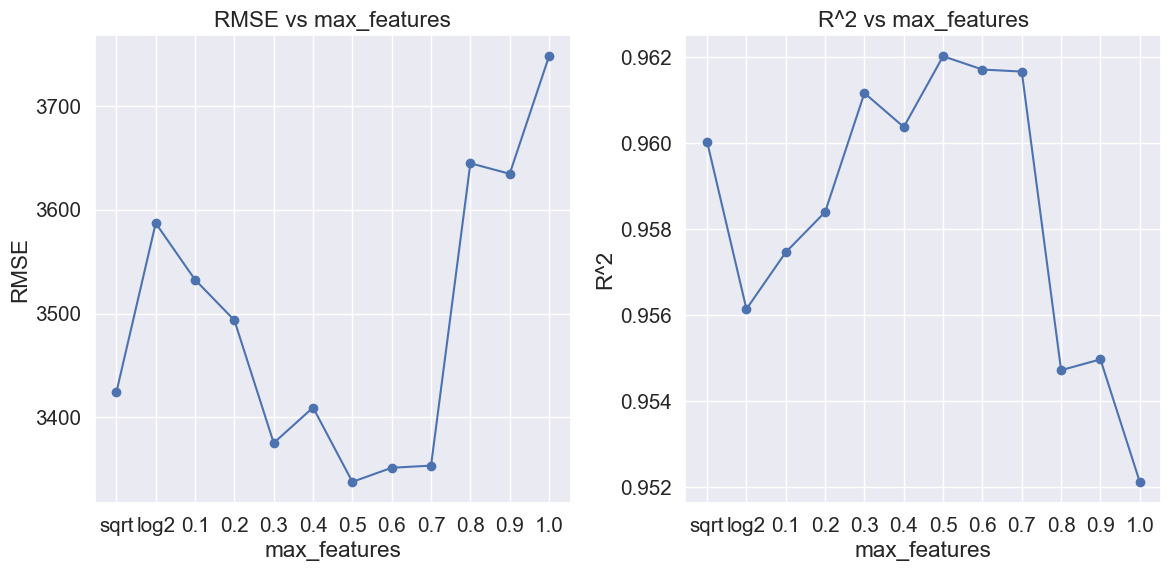
\includegraphics[keepaspectratio]{random_forest_files/figure-pdf/cell-13-output-1.png}}

As observed from the plots, \textbf{Random Forest performs best when
tree decorrelation is balanced}.\\
Setting \texttt{max\_features} too low or too high hurts the model's
generalization ability.

\begin{itemize}
\tightlist
\item
  \textbf{R²} peaks when \texttt{max\_features} is around \textbf{0.5 to
  0.6}, consistent with the lowest RMSE values.
\item
  \textbf{R²} drops at both extremes:

  \begin{itemize}
  \tightlist
  \item
    Using \textbf{too few features} (\texttt{sqrt}, \texttt{log2}, or
    very small proportions) leads to \textbf{underfitting}.
  \item
    Using \textbf{all features} (\texttt{max\_features=1.0}) increases
    correlation between trees, leading to \textbf{overfitting}.
  \end{itemize}
\end{itemize}

\begin{quote}
🔑 \textbf{Key takeaway}: Carefully tuning \texttt{max\_features} is
critical for achieving the best balance between bias and variance in
Random Forest models.
\end{quote}

Let's get the minimum RMSE and the corresponding \texttt{max\_features}
value from the result

\begin{Shaded}
\begin{Highlighting}[]

\NormalTok{min\_rmse }\OperatorTok{=} \BuiltInTok{min}\NormalTok{(rmse\_list)}
\NormalTok{min\_rmse\_index }\OperatorTok{=}\NormalTok{ rmse\_list.index(min\_rmse)}
\NormalTok{best\_max\_feature }\OperatorTok{=}\NormalTok{ max\_features[min\_rmse\_index]}
\BuiltInTok{print}\NormalTok{(}\SpecialStringTok{f\textquotesingle{}Minimum RMSE: }\SpecialCharTok{\{}\NormalTok{min\_rmse}\SpecialCharTok{:.2f\}}\SpecialStringTok{\textquotesingle{}}\NormalTok{)}
\BuiltInTok{print}\NormalTok{(}\SpecialStringTok{f\textquotesingle{}Best max\_features: }\SpecialCharTok{\{}\NormalTok{best\_max\_feature}\SpecialCharTok{\}}\SpecialStringTok{\textquotesingle{}}\NormalTok{)}
\CommentTok{\# get the maximum R\^{}2 and the corresponding max\_features parameter}
\NormalTok{max\_r2 }\OperatorTok{=} \BuiltInTok{max}\NormalTok{(r2\_list)}
\NormalTok{max\_r2\_index }\OperatorTok{=}\NormalTok{ r2\_list.index(max\_r2)}
\NormalTok{best\_max\_feature\_r2 }\OperatorTok{=}\NormalTok{ max\_features[max\_r2\_index]}
\BuiltInTok{print}\NormalTok{(}\SpecialStringTok{f\textquotesingle{}Maximum R\^{}2: }\SpecialCharTok{\{}\NormalTok{max\_r2}\SpecialCharTok{:.2f\}}\SpecialStringTok{\textquotesingle{}}\NormalTok{)}
\BuiltInTok{print}\NormalTok{(}\SpecialStringTok{f\textquotesingle{}Best max\_features: }\SpecialCharTok{\{}\NormalTok{best\_max\_feature\_r2}\SpecialCharTok{\}}\SpecialStringTok{\textquotesingle{}}\NormalTok{)}
\end{Highlighting}
\end{Shaded}

\begin{verbatim}
Minimum RMSE: 3338.02
Best max_features: 0.5
Maximum R^2: 0.96
Best max_features: 0.5
\end{verbatim}

Adjusting \texttt{max\_features} from `sqrt' to 0.5 led to a slight
improvement in RMSE, reducing it from 3424 to 3338

\section{Other Hyperparameters in Random
Forest}\label{other-hyperparameters-in-random-forest}

\subsection{Why Bagging Uses Unpruned
Trees}\label{why-bagging-uses-unpruned-trees}

\begin{itemize}
\tightlist
\item
  Bagging's main strength lies in \textbf{reducing variance}, not bias.
\item
  Deep, unpruned decision trees tend to \textbf{overfit} (high
  variance), but bagging effectively reduces this variance through
  aggregation.
\item
  Using pruned trees reduces variance but \textbf{increases bias} ---
  and since bagging does not correct bias, this would weaken overall
  performance.
\end{itemize}

\begin{quote}
Therefore, in bagging, it is common to let each tree \textbf{grow fully}
to preserve low bias and rely on bagging to reduce variance.
\end{quote}

\subsection{Hyperparameters That Control Tree Complexity in Random
Forest}\label{hyperparameters-that-control-tree-complexity-in-random-forest}

\begin{longtable}[]{@{}
  >{\raggedright\arraybackslash}p{(\linewidth - 4\tabcolsep) * \real{0.3293}}
  >{\raggedright\arraybackslash}p{(\linewidth - 4\tabcolsep) * \real{0.4390}}
  >{\raggedright\arraybackslash}p{(\linewidth - 4\tabcolsep) * \real{0.2317}}@{}}
\toprule\noalign{}
\begin{minipage}[b]{\linewidth}\raggedright
Setting
\end{minipage} & \begin{minipage}[b]{\linewidth}\raggedright
Effect
\end{minipage} & \begin{minipage}[b]{\linewidth}\raggedright
Applies to
\end{minipage} \\
\midrule\noalign{}
\endhead
\bottomrule\noalign{}
\endlastfoot
\texttt{max\_depth=None} & Full trees, low bias, high variance &
Bagging, RF \\
\texttt{max\_depth=some\ int} & Pruned trees, more bias, less variance &
Especially helpful in RF \\
\texttt{min\_samples\_split/leaves} & Prevents small, unreliable
branches & Both \\
\end{longtable}

\subsection{Why Random Forest Often Limits Tree
Depth}\label{why-random-forest-often-limits-tree-depth}

In Random Forest, only a \textbf{subset of features} is considered at
each split.\\
As a result, fully growing trees without any depth constraint can cause
them to \textbf{overfit} to noise within these smaller subsets.

Limiting tree complexity in Random Forest:

\begin{itemize}
\tightlist
\item
  \textbf{Prevents deep trees} from chasing noise and overfitting.
\item
  \textbf{Improves generalization}, especially in high-dimensional or
  noisy datasets.
\item
  \textbf{Balances} the bias-variance tradeoff more effectively than
  using full trees.
\end{itemize}

\begin{quote}
Careful tuning of tree depth and other complexity-controlling
hyperparameters is critical to maximizing Random Forest performance.
\end{quote}

\subsection{Let's Tune Multiple Hyperparameters Simultaneously Using
Cross-Validation}\label{lets-tune-multiple-hyperparameters-simultaneously-using-cross-validation}

Given the number of hyperparameters involved, we will use
\texttt{BayesSearchCV} to efficiently perform tuning.\\
This approach helps reduce computational cost while exploring a wide
range of hyperparameter combinations.

\begin{Shaded}
\begin{Highlighting}[]
\CommentTok{\# hyperparameter tuning for the random forest regressor}

\ImportTok{from}\NormalTok{ skopt.space }\ImportTok{import}\NormalTok{ Integer, Categorical, Real}
\ImportTok{from}\NormalTok{ skopt }\ImportTok{import}\NormalTok{ BayesSearchCV}

\CommentTok{\# Rename the pipeline step for clarity (recommended)}
\NormalTok{random\_forest\_regressor }\OperatorTok{=}\NormalTok{ RandomForestRegressor(}
\NormalTok{    random\_state}\OperatorTok{=}\DecValTok{42}
\NormalTok{)}

\NormalTok{randome\_forest\_pipeline }\OperatorTok{=}\NormalTok{ Pipeline(steps}\OperatorTok{=}\NormalTok{[}
\NormalTok{    (}\StringTok{\textquotesingle{}preprocessor\textquotesingle{}}\NormalTok{, preprocessor),}
\NormalTok{    (}\StringTok{\textquotesingle{}rf\textquotesingle{}}\NormalTok{, random\_forest\_regressor)  }\CommentTok{\# Renamed from \textquotesingle{}bagging\textquotesingle{} to \textquotesingle{}rf\textquotesingle{}}
\NormalTok{])}

\NormalTok{param\_space }\OperatorTok{=}\NormalTok{ \{}
    \CommentTok{\# Tree structure (control complexity)}
    \StringTok{"rf\_\_max\_depth"}\NormalTok{: Integer(}\DecValTok{5}\NormalTok{, }\DecValTok{35}\NormalTok{),  }
    \StringTok{"rf\_\_min\_samples\_split"}\NormalTok{: Integer(}\DecValTok{2}\NormalTok{, }\DecValTok{20}\NormalTok{),}
    \StringTok{"rf\_\_min\_samples\_leaf"}\NormalTok{: Integer(}\DecValTok{1}\NormalTok{, }\DecValTok{10}\NormalTok{),}
    \StringTok{"rf\_\_max\_features"}\NormalTok{: Real(}\FloatTok{0.1}\NormalTok{, }\FloatTok{1.0}\NormalTok{),}
    
    \CommentTok{\# Ensemble settings}
    \StringTok{"rf\_\_n\_estimators"}\NormalTok{: Integer(}\DecValTok{20}\NormalTok{, }\DecValTok{60}\NormalTok{),}
    
    \CommentTok{\# Advanced}
    \StringTok{"rf\_\_max\_samples"}\NormalTok{: Real(}\FloatTok{0.1}\NormalTok{, }\FloatTok{1.0}\NormalTok{),}
\NormalTok{\}}

\NormalTok{opt }\OperatorTok{=}\NormalTok{ BayesSearchCV(}
\NormalTok{    randome\_forest\_pipeline,}
\NormalTok{    param\_space,}
\NormalTok{    n\_iter}\OperatorTok{=}\DecValTok{50}\NormalTok{,  }\CommentTok{\# Adjust based on computational resources}
\NormalTok{    cv}\OperatorTok{=}\DecValTok{5}\NormalTok{,}
\NormalTok{    n\_jobs}\OperatorTok{={-}}\DecValTok{1}\NormalTok{,}
\NormalTok{    random\_state}\OperatorTok{=}\DecValTok{42}
\NormalTok{)}
\NormalTok{opt.fit(X\_train, y\_train)  }

\CommentTok{\# make predictions on the test data}
\NormalTok{y\_pred }\OperatorTok{=}\NormalTok{ opt.predict(X\_test)}
\CommentTok{\# calculate the RMSE and R\^{}2 score}
\NormalTok{rmse }\OperatorTok{=}\NormalTok{ root\_mean\_squared\_error(y\_test, y\_pred)}
\NormalTok{r2 }\OperatorTok{=}\NormalTok{ r2\_score(y\_test, y\_pred)}
\BuiltInTok{print}\NormalTok{(}\SpecialStringTok{f\textquotesingle{}RMSE: }\SpecialCharTok{\{}\NormalTok{rmse}\SpecialCharTok{:.2f\}}\SpecialStringTok{\textquotesingle{}}\NormalTok{)}
\BuiltInTok{print}\NormalTok{(}\SpecialStringTok{f\textquotesingle{}R\^{}2: }\SpecialCharTok{\{}\NormalTok{r2}\SpecialCharTok{:.2f\}}\SpecialStringTok{\textquotesingle{}}\NormalTok{)}
\CommentTok{\# calculate the training rmse and r\^{}2 score}
\NormalTok{y\_train\_pred }\OperatorTok{=}\NormalTok{ opt.predict(X\_train)}
\NormalTok{train\_rmse }\OperatorTok{=}\NormalTok{ root\_mean\_squared\_error(y\_train, y\_train\_pred)}
\NormalTok{train\_r2 }\OperatorTok{=}\NormalTok{ r2\_score(y\_train, y\_train\_pred)}
\BuiltInTok{print}\NormalTok{(}\SpecialStringTok{f\textquotesingle{}Training RMSE: }\SpecialCharTok{\{}\NormalTok{train\_rmse}\SpecialCharTok{:.2f\}}\SpecialStringTok{\textquotesingle{}}\NormalTok{)}
\BuiltInTok{print}\NormalTok{(}\SpecialStringTok{f\textquotesingle{}Training R\^{}2: }\SpecialCharTok{\{}\NormalTok{train\_r2}\SpecialCharTok{:.2f\}}\SpecialStringTok{\textquotesingle{}}\NormalTok{)}
\end{Highlighting}
\end{Shaded}

\begin{verbatim}
RMSE: 3278.42
R^2: 0.96
Training RMSE: 1220.88
Training R^2: 0.99
\end{verbatim}

As observed in the results, RMSE was further reduced after
simultaneously tuning multiple hyperparameters compared to only tuning
\texttt{max\_features} (from 3338 to 3278).\\
However, due to the small and simple nature of the dataset, the
performance improvement is relatively marginal.\\
On larger and more complex datasets, the performance gains from
comprehensive hyperparameter tuning would likely be much more
substantial.

\section{Feature Importance in Random
Forest}\label{feature-importance-in-random-forest}

Random Forest provides a natural way to estimate \textbf{feature
importance}.

Each time a feature is used to split a node, it contributes to reducing
impurity (such as Gini impurity for classification or variance for
regression).\\
By averaging these contributions over all trees in the forest, we can
rank features by how important they are to the model's predictive
performance.

\subsection{How Feature Importance Is
Calculated}\label{how-feature-importance-is-calculated}

\begin{itemize}
\tightlist
\item
  A feature's importance is based on the \textbf{total reduction of the
  criterion} (e.g., variance for regression) it brings across all splits
  it is used in.
\item
  Features that result in larger reductions in impurity are assigned
  \textbf{higher importance scores}.
\item
  The importance scores are \textbf{normalized} so that they sum to 1
  across all features.
\end{itemize}

\subsection{Accessing Feature
Importances}\label{accessing-feature-importances}

After fitting a Random Forest model, feature importances can be accessed
through the attribute:

\begin{Shaded}
\begin{Highlighting}[]
\NormalTok{model.feature\_importances\_}
\end{Highlighting}
\end{Shaded}

\begin{Shaded}
\begin{Highlighting}[]
\CommentTok{\# get numerical\_feature and categorical\_feature from the pipeline}
\NormalTok{num\_features }\OperatorTok{=}\NormalTok{ numerical\_feature}
\NormalTok{cat\_transformer }\OperatorTok{=}\NormalTok{ opt.best\_estimator\_.named\_steps[}\StringTok{\textquotesingle{}preprocessor\textquotesingle{}}\NormalTok{].named\_transformers\_[}\StringTok{\textquotesingle{}cat\textquotesingle{}}\NormalTok{]}
\NormalTok{cat\_features }\OperatorTok{=}\NormalTok{ cat\_transformer.get\_feature\_names\_out(categorical\_feature)}

\CommentTok{\# concatenate all feature names}
\NormalTok{feature\_names }\OperatorTok{=}\NormalTok{ np.concatenate([num\_features, cat\_features])}
\end{Highlighting}
\end{Shaded}

\begin{Shaded}
\begin{Highlighting}[]
\CommentTok{\# output feature importances}

\NormalTok{importances }\OperatorTok{=}\NormalTok{ opt.best\_estimator\_.named\_steps[}\StringTok{\textquotesingle{}rf\textquotesingle{}}\NormalTok{].feature\_importances\_}
\NormalTok{feature\_importances }\OperatorTok{=}\NormalTok{ pd.DataFrame(importances, index}\OperatorTok{=}\NormalTok{feature\_names, columns}\OperatorTok{=}\NormalTok{[}\StringTok{\textquotesingle{}importance\textquotesingle{}}\NormalTok{]).sort\_values(}\StringTok{\textquotesingle{}importance\textquotesingle{}}\NormalTok{, ascending}\OperatorTok{=}\VariableTok{False}\NormalTok{)}

\CommentTok{\# select top 10 features}
\NormalTok{top\_10 }\OperatorTok{=}\NormalTok{ feature\_importances.head(}\DecValTok{10}\NormalTok{)}

\CommentTok{\# plot the top 10 feature importances}
\NormalTok{plt.figure(figsize}\OperatorTok{=}\NormalTok{(}\DecValTok{12}\NormalTok{, }\DecValTok{6}\NormalTok{))}
\NormalTok{plt.barh(top\_10.index[::}\OperatorTok{{-}}\DecValTok{1}\NormalTok{], top\_10[}\StringTok{\textquotesingle{}importance\textquotesingle{}}\NormalTok{][::}\OperatorTok{{-}}\DecValTok{1}\NormalTok{])  }\CommentTok{\# reverse for top{-}to{-}bottom order}
\NormalTok{plt.xlabel(}\StringTok{\textquotesingle{}Importance\textquotesingle{}}\NormalTok{)}
\NormalTok{plt.title(}\StringTok{\textquotesingle{}Top 10 Feature Importances\textquotesingle{}}\NormalTok{)}
\NormalTok{plt.grid(axis}\OperatorTok{=}\StringTok{\textquotesingle{}x\textquotesingle{}}\NormalTok{)}
\NormalTok{plt.tight\_layout()}
\NormalTok{plt.show()}
\end{Highlighting}
\end{Shaded}

\pandocbounded{\includegraphics[keepaspectratio]{random_forest_files/figure-pdf/cell-17-output-1.png}}

\section{In Summary}\label{in-summary}

Random Forest is a special case of bagging.\\
The \texttt{n\_estimators} and \texttt{oob\_score} hyperparameters
function similarly in both methods, helping to aggregate multiple
decision trees into a strong ensemble.

In this notebook, we focused on the key differences between
\textbf{Random Forest} and \textbf{standard bagging}.\\
Random Forest generally outperforms bagging by introducing an additional
layer of randomness:\\
at each split, only a \textbf{random subset of features} is
considered.\\
This strategy \textbf{decorrelates} the individual trees,
\textbf{increases diversity} within the ensemble, and \textbf{further
reduces variance}, leading to stronger generalization performance.

\begin{quote}
🎯 \textbf{Key takeaway}: Bagging reduces variance by aggregating
independent models, while Random Forest improves further by
strategically injecting feature-level randomness to strengthen ensemble
diversity.
\end{quote}

\section{Next Step}\label{next-step}

In the next section, we will explore \textbf{Boosting methods},\\
where models are built \textbf{sequentially}, each one focusing on
correcting the errors made by the previous models.\\
Boosting shifts the focus from reducing variance to \textbf{reducing
bias}, offering another powerful strategy for improving model
performance.

\chapter{Adaptive Boosting}\label{adaptive-boosting}

After learning how Bagging and Random Forest reduce variance by
aggregating many trees,\\
we now turn to a different strategy: \textbf{Boosting}.

\textbf{Boosting} builds trees \textbf{sequentially}, with each new tree
focusing on correcting the mistakes made by the previous ones.

\emph{Read section 8.2.3 of the book before using these notes.}

For the exact algorithms underlying the AdaBoost algorithm, check out
the papers
\href{https://citeseerx.ist.psu.edu/document?repid=rep1&type=pdf&doi=6d8226a52ebc70c8d97ccae10a74e1b0a3908ec1}{\texttt{AdaBoostRegressor()}}
and
\href{https://dept.stat.lsa.umich.edu/~jizhu/pubs/Zhu-SII09.pdf}{\texttt{AdaBoostClassifier()}}.

\begin{Shaded}
\begin{Highlighting}[]
\ImportTok{import}\NormalTok{ pandas }\ImportTok{as}\NormalTok{ pd}
\ImportTok{import}\NormalTok{ numpy }\ImportTok{as}\NormalTok{ np}
\ImportTok{import}\NormalTok{ seaborn }\ImportTok{as}\NormalTok{ sns}
\ImportTok{import}\NormalTok{ matplotlib.pyplot }\ImportTok{as}\NormalTok{ plt}
\ImportTok{from}\NormalTok{ sklearn.metrics }\ImportTok{import}\NormalTok{ mean\_squared\_error}
\ImportTok{from}\NormalTok{ sklearn.model\_selection }\ImportTok{import}\NormalTok{ cross\_val\_score,train\_test\_split, KFold, cross\_val\_predict}
\ImportTok{from}\NormalTok{ sklearn.metrics }\ImportTok{import}\NormalTok{ root\_mean\_squared\_error,r2\_score,roc\_curve,auc,precision\_recall\_curve, accuracy\_score, }\OperatorTok{\textbackslash{}}
\NormalTok{recall\_score, precision\_score, confusion\_matrix}
\ImportTok{from}\NormalTok{ sklearn.tree }\ImportTok{import}\NormalTok{ DecisionTreeRegressor,DecisionTreeClassifier}
\ImportTok{from}\NormalTok{ sklearn.model\_selection }\ImportTok{import}\NormalTok{ GridSearchCV, ParameterGrid, StratifiedKFold}
\ImportTok{from}\NormalTok{ sklearn.ensemble }\ImportTok{import}\NormalTok{ BaggingRegressor,BaggingClassifier,AdaBoostRegressor,AdaBoostClassifier, }\OperatorTok{\textbackslash{}}
\NormalTok{RandomForestRegressor}
\ImportTok{from}\NormalTok{ sklearn.pipeline }\ImportTok{import}\NormalTok{ Pipeline}
\ImportTok{from}\NormalTok{ sklearn.compose }\ImportTok{import}\NormalTok{ ColumnTransformer}
\ImportTok{from}\NormalTok{ sklearn.preprocessing }\ImportTok{import}\NormalTok{ OneHotEncoder, FunctionTransformer}
\ImportTok{import}\NormalTok{ itertools }\ImportTok{as}\NormalTok{ it}
\ImportTok{import}\NormalTok{ time }\ImportTok{as}\NormalTok{ time}

\ImportTok{from}\NormalTok{ skopt }\ImportTok{import}\NormalTok{ BayesSearchCV}
\ImportTok{from}\NormalTok{ skopt.space }\ImportTok{import}\NormalTok{ Real, Categorical, Integer}
\ImportTok{from}\NormalTok{ skopt.plots }\ImportTok{import}\NormalTok{ plot\_objective, plot\_histogram, plot\_convergence}
\ImportTok{import}\NormalTok{ warnings}
\ImportTok{from}\NormalTok{ IPython }\ImportTok{import}\NormalTok{ display}
\end{Highlighting}
\end{Shaded}

\section{What is AdaBoost?}\label{what-is-adaboost}

\textbf{AdaBoost} stands for \textbf{Adaptive Boosting}.\\
It was one of the first boosting algorithms developed.

The core idea behind AdaBoost:

\begin{itemize}
\tightlist
\item
  Train a \textbf{weak learner} (usually a shallow decision tree) on the
  original data.
\item
  Increase the weights of examples that the learner misclassified.
\item
  Train the next learner on this updated, reweighted data.
\item
  Repeat this process, focusing more and more on hard-to-predict
  examples.
\end{itemize}

The final prediction is a \textbf{weighted combination} of all the weak
learners.

\section{AdaBoost Intuition}\label{adaboost-intuition}

\begin{itemize}
\tightlist
\item
  Easy-to-classify points are \textbf{de-emphasized}.
\item
  Hard-to-classify points are \textbf{emphasized}.
\item
  Each learner \textbf{adapts} to the mistakes made by previous learners
  --- hence ``adaptive'' boosting.
\item
  \textbf{Better-performing learners} are given \textbf{higher weight}
  in the final prediction.
\end{itemize}

\begin{quote}
Over time, the model becomes better at handling difficult cases.
\end{quote}

\section{How AdaBoost Works (High-Level
Steps)}\label{how-adaboost-works-high-level-steps}

\begin{enumerate}
\def\labelenumi{\arabic{enumi}.}
\tightlist
\item
  Initialize equal weights for all training examples.
\item
  Train a weak learner (e.g., decision stump).
\item
  Evaluate its performance:

  \begin{itemize}
  \tightlist
  \item
    Increase weights for misclassified points.
  \item
    Decrease weights for correctly classified points.
  \end{itemize}
\item
  Train the next learner using the updated weights.
\item
  Repeat for a set number of learners (\texttt{n\_estimators}).
\item
  Combine all learners into a final weighted model.
\end{enumerate}

\section{Key Hyperparameters in
AdaBoost}\label{key-hyperparameters-in-adaboost}

\begin{longtable}[]{@{}
  >{\raggedright\arraybackslash}p{(\linewidth - 4\tabcolsep) * \real{0.2000}}
  >{\raggedright\arraybackslash}p{(\linewidth - 4\tabcolsep) * \real{0.6000}}
  >{\raggedright\arraybackslash}p{(\linewidth - 4\tabcolsep) * \real{0.2000}}@{}}
\toprule\noalign{}
\begin{minipage}[b]{\linewidth}\raggedright
Hyperparameter
\end{minipage} & \begin{minipage}[b]{\linewidth}\raggedright
Meaning
\end{minipage} & \begin{minipage}[b]{\linewidth}\raggedright
Typical Values
\end{minipage} \\
\midrule\noalign{}
\endhead
\bottomrule\noalign{}
\endlastfoot
\texttt{n\_estimators} & Number of weak learners & 50--500 \\
\texttt{learning\_rate} & Shrinks each learner's contribution &
0.01--1.0 \\
\texttt{estimator} & Type of weak learner (default: decision stump) &
Shallow trees \\
\end{longtable}

\begin{itemize}
\tightlist
\item
  \textbf{Lowering \texttt{learning\_rate}} typically requires
  \textbf{more estimators} but improves generalization.
\end{itemize}

\section{AdaBoost for Regression}\label{adaboost-for-regression}

We will revisit the car dataset we used earlier and evaluate how
AdaBoost performs compared to a single decision tree and a bagging
ensemble

\begin{Shaded}
\begin{Highlighting}[]
\CommentTok{\# Load the dataset}
\NormalTok{car }\OperatorTok{=}\NormalTok{ pd.read\_csv(}\StringTok{\textquotesingle{}Datasets/car.csv\textquotesingle{}}\NormalTok{)}
\NormalTok{car.head()}
\end{Highlighting}
\end{Shaded}

\begin{longtable}[]{@{}lllllllllll@{}}
\toprule\noalign{}
& brand & model & year & transmission & mileage & fuelType & tax & mpg &
engineSize & price \\
\midrule\noalign{}
\endhead
\bottomrule\noalign{}
\endlastfoot
0 & vw & Beetle & 2014 & Manual & 55457 & Diesel & 30 & 65.3266 & 1.6 &
7490 \\
1 & vauxhall & GTC & 2017 & Manual & 15630 & Petrol & 145 & 47.2049 &
1.4 & 10998 \\
2 & merc & G Class & 2012 & Automatic & 43000 & Diesel & 570 & 25.1172 &
3.0 & 44990 \\
3 & audi & RS5 & 2019 & Automatic & 10 & Petrol & 145 & 30.5593 & 2.9 &
51990 \\
4 & merc & X-CLASS & 2018 & Automatic & 14000 & Diesel & 240 & 35.7168 &
2.3 & 28990 \\
\end{longtable}

\begin{Shaded}
\begin{Highlighting}[]
\BuiltInTok{print}\NormalTok{(car.info())}
\end{Highlighting}
\end{Shaded}

\begin{verbatim}
<class 'pandas.core.frame.DataFrame'>
RangeIndex: 7632 entries, 0 to 7631
Data columns (total 10 columns):
 #   Column        Non-Null Count  Dtype  
---  ------        --------------  -----  
 0   brand         7632 non-null   object 
 1   model         7632 non-null   object 
 2   year          7632 non-null   int64  
 3   transmission  7632 non-null   object 
 4   mileage       7632 non-null   int64  
 5   fuelType      7632 non-null   object 
 6   tax           7632 non-null   int64  
 7   mpg           7632 non-null   float64
 8   engineSize    7632 non-null   float64
 9   price         7632 non-null   int64  
dtypes: float64(2), int64(4), object(4)
memory usage: 596.4+ KB
None
\end{verbatim}

\begin{Shaded}
\begin{Highlighting}[]
\NormalTok{X }\OperatorTok{=}\NormalTok{ car.drop(columns}\OperatorTok{=}\NormalTok{[}\StringTok{\textquotesingle{}price\textquotesingle{}}\NormalTok{])}
\NormalTok{y }\OperatorTok{=}\NormalTok{ car[}\StringTok{\textquotesingle{}price\textquotesingle{}}\NormalTok{]}

\NormalTok{X\_train, X\_test, y\_train, y\_test }\OperatorTok{=}\NormalTok{ train\_test\_split(X, y, test\_size}\OperatorTok{=}\FloatTok{0.2}\NormalTok{, random\_state}\OperatorTok{=}\DecValTok{42}\NormalTok{)}

\CommentTok{\# extract the categorical columns and put them in a list}
\NormalTok{categorical\_feature }\OperatorTok{=}\NormalTok{ X.select\_dtypes(include}\OperatorTok{=}\NormalTok{[}\StringTok{\textquotesingle{}object\textquotesingle{}}\NormalTok{]).columns.tolist()}

\CommentTok{\# extract the numerical columns and put them in a list}
\NormalTok{numerical\_feature }\OperatorTok{=}\NormalTok{ X.select\_dtypes(include}\OperatorTok{=}\NormalTok{[}\StringTok{\textquotesingle{}int64\textquotesingle{}}\NormalTok{, }\StringTok{\textquotesingle{}float64\textquotesingle{}}\NormalTok{]).columns.tolist()}
\end{Highlighting}
\end{Shaded}

\begin{Shaded}
\begin{Highlighting}[]
\NormalTok{encoder }\OperatorTok{=}\NormalTok{ OneHotEncoder(handle\_unknown}\OperatorTok{=}\StringTok{\textquotesingle{}ignore\textquotesingle{}}\NormalTok{, sparse\_output}\OperatorTok{=}\VariableTok{False}\NormalTok{)}

\NormalTok{X\_train\_encoded }\OperatorTok{=}\NormalTok{ encoder.fit\_transform(X\_train[categorical\_feature])}
\NormalTok{X\_test\_encoded }\OperatorTok{=}\NormalTok{ encoder.transform(X\_test[categorical\_feature])}

\CommentTok{\# Convert the encoded features back to DataFrame}
\NormalTok{X\_train\_encoded\_df }\OperatorTok{=}\NormalTok{ pd.DataFrame(X\_train\_encoded, columns}\OperatorTok{=}\NormalTok{encoder.get\_feature\_names\_out(categorical\_feature))}
\NormalTok{X\_test\_encoded\_df }\OperatorTok{=}\NormalTok{ pd.DataFrame(X\_test\_encoded, columns}\OperatorTok{=}\NormalTok{encoder.get\_feature\_names\_out(categorical\_feature))}

\CommentTok{\# Concatenate the encoded features with the original numerical features}
\NormalTok{X\_train\_final }\OperatorTok{=}\NormalTok{ pd.concat([X\_train\_encoded\_df, X\_train[numerical\_feature].reset\_index(drop}\OperatorTok{=}\VariableTok{True}\NormalTok{)], axis}\OperatorTok{=}\DecValTok{1}\NormalTok{)}
\NormalTok{X\_test\_final }\OperatorTok{=}\NormalTok{ pd.concat([X\_test\_encoded\_df, X\_test[numerical\_feature].reset\_index(drop}\OperatorTok{=}\VariableTok{True}\NormalTok{)], axis}\OperatorTok{=}\DecValTok{1}\NormalTok{)}
\end{Highlighting}
\end{Shaded}

\subsection{Let's build a adaboost regressor model with default
settings}\label{lets-build-a-adaboost-regressor-model-with-default-settings}

\begin{Shaded}
\begin{Highlighting}[]

\CommentTok{\# build a adaboost regressor model with default parameters}
\NormalTok{adaboost\_regressor }\OperatorTok{=}\NormalTok{ AdaBoostRegressor(random\_state}\OperatorTok{=}\DecValTok{0}\NormalTok{)}

\CommentTok{\# fit the model}
\NormalTok{adaboost\_regressor.fit(X\_train\_final, y\_train)}

\CommentTok{\# predict the test set}
\NormalTok{y\_pred }\OperatorTok{=}\NormalTok{ adaboost\_regressor.predict(X\_test\_final)}

\CommentTok{\# calculate the mean squared error}
\NormalTok{rmse }\OperatorTok{=}\NormalTok{ root\_mean\_squared\_error(y\_test, y\_pred)}
\BuiltInTok{print}\NormalTok{(}\SpecialStringTok{f\textquotesingle{}RMSE: }\SpecialCharTok{\{}\NormalTok{rmse}\SpecialCharTok{:.2f\}}\SpecialStringTok{\textquotesingle{}}\NormalTok{)}
\BuiltInTok{print}\NormalTok{(}\SpecialStringTok{f\textquotesingle{}R2 Score: }\SpecialCharTok{\{}\NormalTok{r2\_score(y\_test, y\_pred)}\SpecialCharTok{\}}\SpecialStringTok{\textquotesingle{}}\NormalTok{)}


\CommentTok{\# calculate the RMSE and R\^{}2 score for the training data}
\NormalTok{y\_pred\_train }\OperatorTok{=}\NormalTok{ adaboost\_regressor.predict(X\_train\_final)}
\NormalTok{rmse\_train }\OperatorTok{=}\NormalTok{ root\_mean\_squared\_error(y\_train, y\_pred\_train)}
\NormalTok{r2\_train }\OperatorTok{=}\NormalTok{ r2\_score(y\_train, y\_pred\_train)}
\BuiltInTok{print}\NormalTok{(}\SpecialStringTok{f\textquotesingle{}Adaboost Train RMSE: }\SpecialCharTok{\{}\NormalTok{rmse\_train}\SpecialCharTok{:.2f\}}\SpecialStringTok{\textquotesingle{}}\NormalTok{)}
\BuiltInTok{print}\NormalTok{(}\SpecialStringTok{f\textquotesingle{}Adaboost Train R\^{}2: }\SpecialCharTok{\{}\NormalTok{r2\_train}\SpecialCharTok{:.2f\}}\SpecialStringTok{\textquotesingle{}}\NormalTok{)}

\CommentTok{\# calculate the test score}
\end{Highlighting}
\end{Shaded}

\begin{verbatim}
RMSE: 10239.74
R2 Score: 0.6426025126917443
Adaboost Train RMSE: 10081.26
Adaboost Train R^2: 0.62
\end{verbatim}

\subsubsection{❓ Why AdaBoost Perform Worse
Here}\label{why-adaboost-perform-worse-here}

\begin{itemize}
\item
  \textbf{Default base estimator is very weak}:\\
  By default, AdaBoost uses \textbf{Decision Stumps}
  (\texttt{DecisionTreeRegressor(max\_depth=1)}), which are extremely
  shallow and tend to \textbf{underfit} the data badly.
\item
  \textbf{Learning rate (\texttt{learning\_rate=1.0}) is too
  aggressive}:\\
  When using very weak learners, a high learning rate can cause the
  boosting process to \textbf{fail to properly build up model strength},
  leading to poor performance.
\item
  \textbf{Dataset characteristics}:\\
  This dataset is \textbf{small} and \textbf{not very noisy}, using very
  shallow trees combined with a high learning rate can cause
  \textbf{severe underfitting}.
\end{itemize}

What should we do next to reduce bias

\begin{itemize}
\tightlist
\item
  Use deeper Trees as Base Learners
\item
  Tune Learning Rate
\item
  Increase the Number of Estimators
\end{itemize}

\subsection{Impact of Tree Depth}\label{impact-of-tree-depth}

By default, AdaBoost uses shallow decision stumps
(\texttt{max\_depth=1}) as weak learners.\\
However, slightly increasing the tree depth can make each learner more
expressive,\\
helping the ensemble capture more complex patterns in the data.

This often leads to a \textbf{reduction in cross-validation RMSE} and
improved model performance,\\
especially when the underlying relationships in the data are non-linear.

From our previous exploration, we found that the fully grown decision
tree has a depth of 34 on this dataset.\\
In this section, we'll experiment with limiting the tree depth and
observe how it affects the model's RMSE.\\
The goal is to find a depth that balances \textbf{bias and variance},
leading to better generalization.

\begin{Shaded}
\begin{Highlighting}[]
\CommentTok{\# get a list of models to evaluate}
\KeywordTok{def}\NormalTok{ get\_models():}
\NormalTok{    models }\OperatorTok{=} \BuiltInTok{dict}\NormalTok{()}
    \CommentTok{\# explore depths from 1 to 10}
    \ControlFlowTok{for}\NormalTok{ i }\KeywordTok{in} \BuiltInTok{range}\NormalTok{(}\DecValTok{1}\NormalTok{,}\DecValTok{34}\NormalTok{):}
        \CommentTok{\# define base model}
\NormalTok{        base }\OperatorTok{=}\NormalTok{ DecisionTreeRegressor(max\_depth}\OperatorTok{=}\NormalTok{i)}
        \CommentTok{\# define ensemble model}
\NormalTok{        models[}\BuiltInTok{str}\NormalTok{(i)] }\OperatorTok{=}\NormalTok{ AdaBoostRegressor(estimator}\OperatorTok{=}\NormalTok{base,n\_estimators}\OperatorTok{=}\DecValTok{100}\NormalTok{, learning\_rate}\OperatorTok{=}\FloatTok{0.1}\NormalTok{, random\_state}\OperatorTok{=}\DecValTok{0}\NormalTok{)}
    \ControlFlowTok{return}\NormalTok{ models}

\CommentTok{\# evaluate a given model using cross{-}validation}
\KeywordTok{def}\NormalTok{ evaluate\_model(model, X, y):}
    \CommentTok{\# define the evaluation procedure}
\NormalTok{    cv }\OperatorTok{=}\NormalTok{ KFold(n\_splits}\OperatorTok{=}\DecValTok{10}\NormalTok{, shuffle}\OperatorTok{=}\VariableTok{True}\NormalTok{, random\_state}\OperatorTok{=}\DecValTok{1}\NormalTok{)}
    \CommentTok{\# evaluate the model and collect the results}
\NormalTok{    scores }\OperatorTok{=} \OperatorTok{{-}}\NormalTok{cross\_val\_score(model, X, y, scoring}\OperatorTok{=}\StringTok{\textquotesingle{}neg\_root\_mean\_squared\_error\textquotesingle{}}\NormalTok{, cv}\OperatorTok{=}\NormalTok{cv, n\_jobs}\OperatorTok{={-}}\DecValTok{1}\NormalTok{)}
    \ControlFlowTok{return}\NormalTok{ scores}

\CommentTok{\# get the models to evaluate}
\NormalTok{models }\OperatorTok{=}\NormalTok{ get\_models()}
\CommentTok{\# evaluate the models and store results}
\NormalTok{results, names }\OperatorTok{=} \BuiltInTok{list}\NormalTok{(), }\BuiltInTok{list}\NormalTok{()}
\ControlFlowTok{for}\NormalTok{ name, model }\KeywordTok{in}\NormalTok{ models.items():}
    \CommentTok{\# evaluate the model}
\NormalTok{    scores }\OperatorTok{=}\NormalTok{ evaluate\_model(model, X\_train\_final, y\_train)}
    \CommentTok{\# store the results}
\NormalTok{    results.append(scores)}
\NormalTok{    names.append(name)}
    \CommentTok{\# summarize the performance along the way}
    \BuiltInTok{print}\NormalTok{(}\StringTok{\textquotesingle{}\textgreater{}}\SpecialCharTok{\%s}\StringTok{ }\SpecialCharTok{\%.3f}\StringTok{ (}\SpecialCharTok{\%.3f}\StringTok{)\textquotesingle{}} \OperatorTok{\%}\NormalTok{ (name, np.mean(scores), np.std(scores)))}
\NormalTok{plt.boxplot(results, labels}\OperatorTok{=}\NormalTok{names, showmeans}\OperatorTok{=}\VariableTok{True}\NormalTok{)}
\NormalTok{plt.ylabel(}\StringTok{\textquotesingle{}Cross validation error\textquotesingle{}}\NormalTok{,fontsize}\OperatorTok{=}\DecValTok{15}\NormalTok{)}
\NormalTok{plt.xlabel(}\StringTok{\textquotesingle{}Depth of each tree\textquotesingle{}}\NormalTok{,fontsize}\OperatorTok{=}\DecValTok{15}\NormalTok{)}\OperatorTok{;}
\end{Highlighting}
\end{Shaded}

\begin{verbatim}
>1 13770.872 (518.361)
>2 9673.586 (398.116)
>3 7783.875 (393.200)
>4 6686.293 (253.234)
>5 5575.918 (176.859)
>6 5106.235 (342.995)
>7 4695.491 (353.584)
>8 4395.372 (366.340)
>9 4143.296 (422.938)
>10 4064.871 (414.840)
>11 3880.994 (433.105)
>12 3831.714 (396.971)
>13 3773.891 (437.190)
>14 3771.442 (425.043)
>15 3769.082 (388.875)
>16 3741.356 (394.563)
>17 3740.153 (415.062)
>18 3721.954 (444.760)
>19 3765.976 (425.594)
>20 3777.496 (425.025)
>21 3827.491 (434.580)
>22 3761.119 (409.760)
>23 3773.776 (429.259)
>24 3763.150 (408.907)
>25 3763.396 (417.512)
>26 3782.507 (405.136)
>27 3791.885 (446.067)
>28 3812.705 (406.567)
>29 3792.121 (445.264)
>30 3780.123 (429.651)
>31 3739.596 (472.987)
>32 3797.480 (426.929)
>33 3754.727 (417.368)
\end{verbatim}

\pandocbounded{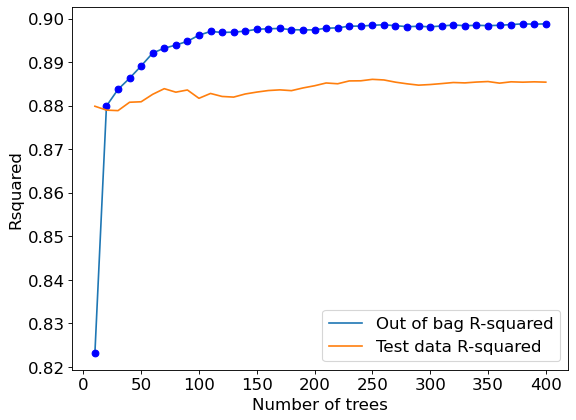
\includegraphics[keepaspectratio]{adaboost_files/figure-pdf/cell-8-output-2.png}}

As shown in the plot, very shallow trees (e.g., \texttt{max\_depth=1} to
\texttt{3}) result in high cross-validation error due to underfitting.\\
As tree depth increases, the model becomes more expressive, and the
error drops sharply up to around depth 10.

Beyond this point, deeper trees offer diminishing returns, and
performance stabilizes.\\
\textgreater{} 🔍 This suggests that \textbf{slightly deeper trees
(e.g., depth 5--10)} strike a good balance between model complexity and
generalization in AdaBoost.

\subsection{Impact of Learning Rate}\label{impact-of-learning-rate}

In boosting algorithms such as \textbf{AdaBoost} or \textbf{Gradient
Boosting}, the \texttt{learning\_rate} controls \textbf{how much each
new tree contributes} to the overall model.

Each new tree makes a correction to the current prediction, and the
learning rate scales \textbf{how aggressively} that correction is
applied.

\begin{itemize}
\tightlist
\item
  🔺 A \textbf{high learning rate} takes \textbf{large correction steps}
  --- fast learning, but higher risk of overshooting or overfitting.
\item
  🔹 A \textbf{low learning rate} takes \textbf{small correction steps}
  --- more stable, but may underfit unless paired with enough trees.
\end{itemize}

\subsubsection{Effect on Performance}\label{effect-on-performance}

\begin{longtable}[]{@{}
  >{\raggedright\arraybackslash}p{(\linewidth - 4\tabcolsep) * \real{0.2800}}
  >{\raggedright\arraybackslash}p{(\linewidth - 4\tabcolsep) * \real{0.3700}}
  >{\raggedright\arraybackslash}p{(\linewidth - 4\tabcolsep) * \real{0.3500}}@{}}
\toprule\noalign{}
\begin{minipage}[b]{\linewidth}\raggedright
Learning Rate
\end{minipage} & \begin{minipage}[b]{\linewidth}\raggedright
Behavior
\end{minipage} & \begin{minipage}[b]{\linewidth}\raggedright
Risk
\end{minipage} \\
\midrule\noalign{}
\endhead
\bottomrule\noalign{}
\endlastfoot
Very Small (e.g., 0.01) & Learns slowly, needs many trees & Underfitting
if not enough trees \\
Moderate (e.g., 0.1--0.2) & Balanced correction, stable learning & Often
optimal \\
Large (e.g., 0.5--1.0) & Learns quickly, may overshoot & Overfitting or
unstable learning \\
\end{longtable}

\begin{quote}
\textbf{Key takeaway}: Small learning rates usually generalize better
--- especially when combined with more estimators.
\end{quote}

\begin{Shaded}
\begin{Highlighting}[]
\KeywordTok{def}\NormalTok{ get\_models():}
\NormalTok{    models }\OperatorTok{=} \BuiltInTok{dict}\NormalTok{()}
\NormalTok{    learning\_rates }\OperatorTok{=}\NormalTok{ [}\FloatTok{0.01}\NormalTok{, }\FloatTok{0.02}\NormalTok{, }\FloatTok{0.04}\NormalTok{, }\FloatTok{0.08}\NormalTok{, }\FloatTok{0.1}\NormalTok{, }\FloatTok{0.15}\NormalTok{, }\FloatTok{0.2}\NormalTok{, }\FloatTok{0.3}\NormalTok{, }\FloatTok{0.6}\NormalTok{, }\FloatTok{1.0}\NormalTok{]}
    \ControlFlowTok{for}\NormalTok{ i }\KeywordTok{in} \BuiltInTok{range}\NormalTok{(}\BuiltInTok{len}\NormalTok{(learning\_rates)):}
\NormalTok{        key }\OperatorTok{=}\NormalTok{ learning\_rates[i]}
\NormalTok{        models[key] }\OperatorTok{=}\NormalTok{ AdaBoostRegressor(learning\_rate}\OperatorTok{=}\NormalTok{learning\_rates[i])}
    \ControlFlowTok{return}\NormalTok{ models}

\CommentTok{\# evaluate a given model using cross{-}validation}
\KeywordTok{def}\NormalTok{ evaluate\_model(model, X, y):}
    \CommentTok{\# define the evaluation procedure}
\NormalTok{    cv }\OperatorTok{=}\NormalTok{ KFold(n\_splits}\OperatorTok{=}\DecValTok{10}\NormalTok{, shuffle}\OperatorTok{=}\VariableTok{True}\NormalTok{, random\_state}\OperatorTok{=}\DecValTok{1}\NormalTok{)}
    \CommentTok{\# evaluate the model and collect the results}
\NormalTok{    scores }\OperatorTok{=} \OperatorTok{{-}}\NormalTok{cross\_val\_score(model, X, y, scoring}\OperatorTok{=}\StringTok{\textquotesingle{}neg\_root\_mean\_squared\_error\textquotesingle{}}\NormalTok{, cv}\OperatorTok{=}\NormalTok{cv, n\_jobs}\OperatorTok{={-}}\DecValTok{1}\NormalTok{)}
    \ControlFlowTok{return}\NormalTok{ scores}

\CommentTok{\# get the models to evaluate}
\NormalTok{models }\OperatorTok{=}\NormalTok{ get\_models()}
\CommentTok{\# evaluate the models and store results}
\NormalTok{results, names }\OperatorTok{=} \BuiltInTok{list}\NormalTok{(), }\BuiltInTok{list}\NormalTok{()}
\ControlFlowTok{for}\NormalTok{ name, model }\KeywordTok{in}\NormalTok{ models.items():}
    \CommentTok{\# evaluate the model}
\NormalTok{    scores }\OperatorTok{=}\NormalTok{ evaluate\_model(model, X\_train\_final, y\_train)}
    \CommentTok{\# store the results}
\NormalTok{    results.append(scores)}
\NormalTok{    names.append(name)}
    \CommentTok{\# summarize the performance along the way}
    \BuiltInTok{print}\NormalTok{(}\StringTok{\textquotesingle{}\textgreater{}}\SpecialCharTok{\%s}\StringTok{ }\SpecialCharTok{\%.1f}\StringTok{ (}\SpecialCharTok{\%.1f}\StringTok{)\textquotesingle{}} \OperatorTok{\%}\NormalTok{ (name, np.mean(scores), np.std(scores)))}
\CommentTok{\# plot model performance for comparison}
\NormalTok{plt.figure(figsize}\OperatorTok{=}\NormalTok{(}\DecValTok{7}\NormalTok{, }\DecValTok{7}\NormalTok{))}
\NormalTok{plt.boxplot(results, labels}\OperatorTok{=}\NormalTok{names, showmeans}\OperatorTok{=}\VariableTok{True}\NormalTok{)}
\NormalTok{plt.ylabel(}\StringTok{\textquotesingle{}Cross validation error\textquotesingle{}}\NormalTok{,fontsize}\OperatorTok{=}\DecValTok{15}\NormalTok{)}
\NormalTok{plt.xlabel(}\StringTok{\textquotesingle{}Learning rate\textquotesingle{}}\NormalTok{,fontsize}\OperatorTok{=}\DecValTok{15}\NormalTok{)}\OperatorTok{;}
\end{Highlighting}
\end{Shaded}

\begin{verbatim}
>0.01 8877.6 (725.1)
>0.02 8797.2 (656.7)
>0.04 8554.4 (540.3)
>0.08 7988.1 (479.9)
>0.1 7763.7 (345.8)
>0.15 7754.0 (380.3)
>0.2 7862.9 (368.8)
>0.3 8024.6 (345.3)
>0.6 9078.9 (205.6)
>1.0 10508.4 (507.6)
\end{verbatim}

\pandocbounded{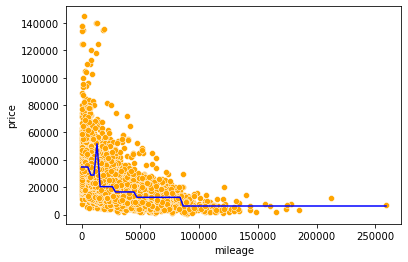
\includegraphics[keepaspectratio]{adaboost_files/figure-pdf/cell-9-output-2.png}}

The plot shows that moderate learning rates (0.1--0.2) yield the best
and most stable model performance, while very small or very large values
hurt generalization --- likely due to underfitting or overfitting.

\subsection{Impact of Number of Trees in
Boosting}\label{impact-of-number-of-trees-in-boosting}

As the number of trees increases in a boosting model, the
\textbf{prediction bias tends to decrease}, while the \textbf{variance
may increase}.

This creates a trade-off:

\begin{itemize}
\tightlist
\item
  Too few trees → underfitting (high bias)\\
\item
  Too many trees → potential overfitting (high variance)
\end{itemize}

\begin{quote}
There is typically an \textbf{optimal number of trees} that minimizes
the overall prediction error, which can be identified using
cross-validation.
\end{quote}

\begin{Shaded}
\begin{Highlighting}[]
\KeywordTok{def}\NormalTok{ get\_models():}
\NormalTok{    models }\OperatorTok{=} \BuiltInTok{dict}\NormalTok{()}
    \CommentTok{\# define number of trees to consider}
\NormalTok{    n\_trees }\OperatorTok{=}\NormalTok{ [}\DecValTok{10}\NormalTok{, }\DecValTok{20}\NormalTok{, }\DecValTok{30}\NormalTok{, }\DecValTok{40}\NormalTok{,  }\DecValTok{50}\NormalTok{, }\DecValTok{60}\NormalTok{, }\DecValTok{70}\NormalTok{,  }\DecValTok{80}\NormalTok{, }\DecValTok{90}\NormalTok{, }\DecValTok{100}\NormalTok{,  }\DecValTok{200}\NormalTok{, }\DecValTok{300}\NormalTok{, }\DecValTok{500}\NormalTok{]}
    \ControlFlowTok{for}\NormalTok{ n }\KeywordTok{in}\NormalTok{ n\_trees:}
\NormalTok{        models[}\BuiltInTok{str}\NormalTok{(n)] }\OperatorTok{=}\NormalTok{ AdaBoostRegressor(n\_estimators}\OperatorTok{=}\NormalTok{n,random\_state}\OperatorTok{=}\DecValTok{1}\NormalTok{, learning\_rate}\OperatorTok{=}\FloatTok{0.1}\NormalTok{)}
    \ControlFlowTok{return}\NormalTok{ models}

\CommentTok{\# evaluate a given model using cross{-}validation}
\KeywordTok{def}\NormalTok{ evaluate\_model(model, X, y):}
    \CommentTok{\# define the evaluation procedure}
\NormalTok{    cv }\OperatorTok{=}\NormalTok{ KFold(n\_splits}\OperatorTok{=}\DecValTok{5}\NormalTok{, shuffle}\OperatorTok{=}\VariableTok{True}\NormalTok{, random\_state}\OperatorTok{=}\DecValTok{1}\NormalTok{)}
    \CommentTok{\# evaluate the model and collect the results}
\NormalTok{    scores }\OperatorTok{=} \OperatorTok{{-}}\NormalTok{cross\_val\_score(model, X, y, scoring}\OperatorTok{=}\StringTok{\textquotesingle{}neg\_root\_mean\_squared\_error\textquotesingle{}}\NormalTok{, cv}\OperatorTok{=}\NormalTok{cv, n\_jobs}\OperatorTok{={-}}\DecValTok{1}\NormalTok{)}
    \ControlFlowTok{return}\NormalTok{ scores}

\CommentTok{\# get the models to evaluate}
\NormalTok{models }\OperatorTok{=}\NormalTok{ get\_models()}
\CommentTok{\# evaluate the models and store results}
\NormalTok{results, names }\OperatorTok{=} \BuiltInTok{list}\NormalTok{(), }\BuiltInTok{list}\NormalTok{()}
\ControlFlowTok{for}\NormalTok{ name, model }\KeywordTok{in}\NormalTok{ models.items():}
    \CommentTok{\# evaluate the model}
\NormalTok{    scores }\OperatorTok{=}\NormalTok{ evaluate\_model(model, X\_train\_final, y\_train)}
    \CommentTok{\# store the results}
\NormalTok{    results.append(scores)}
\NormalTok{    names.append(name)}
    \CommentTok{\# summarize the performance along the way}
    \BuiltInTok{print}\NormalTok{(}\StringTok{\textquotesingle{}\textgreater{}}\SpecialCharTok{\%s}\StringTok{ }\SpecialCharTok{\%.3f}\StringTok{ (}\SpecialCharTok{\%.3f}\StringTok{)\textquotesingle{}} \OperatorTok{\%}\NormalTok{ (name, np.mean(scores), np.std(scores)))}
\CommentTok{\# plot model performance for comparison}
\NormalTok{plt.boxplot(results, labels}\OperatorTok{=}\NormalTok{names, showmeans}\OperatorTok{=}\VariableTok{True}\NormalTok{)}
\NormalTok{plt.ylabel(}\StringTok{\textquotesingle{}Cross validation error\textquotesingle{}}\NormalTok{,fontsize}\OperatorTok{=}\DecValTok{15}\NormalTok{)}
\NormalTok{plt.xlabel(}\StringTok{\textquotesingle{}Number of trees\textquotesingle{}}\NormalTok{,fontsize}\OperatorTok{=}\DecValTok{15}\NormalTok{)}\OperatorTok{;}
\end{Highlighting}
\end{Shaded}

\begin{verbatim}
>10 8901.126 (529.620)
>20 8640.382 (495.164)
>30 8328.349 (539.563)
>40 7972.809 (387.803)
>50 7907.280 (359.779)
>60 7927.212 (305.995)
>70 7904.131 (281.108)
>80 7914.196 (295.777)
>90 7917.841 (274.357)
>100 7927.393 (260.542)
>200 8286.386 (180.913)
>300 8884.444 (230.006)
>500 10024.047 (421.340)
\end{verbatim}

\pandocbounded{\includegraphics[keepaspectratio]{adaboost_files/figure-pdf/cell-10-output-2.png}}

With a learning rate of 0.1, the validation error initially decreases,
then levels off, and eventually starts to increase --- indicating that
overfitting is beginning to occur

\subsection{Tuning Hyperparameters
Simultaneously}\label{tuning-hyperparameters-simultaneously}

In the following section, we will use \textbf{BayesSearchCV} instead of
\texttt{GridSearchCV} to efficiently tune multiple hyperparameters at
once.\\
Unlike grid search, which exhaustively evaluates all combinations,
Bayesian optimization intelligently explores the hyperparameter space by
learning from previous evaluations.\\
This allows us to find a high-performing model using \textbf{fewer
iterations and less computation}.

\begin{Shaded}
\begin{Highlighting}[]
\ImportTok{from}\NormalTok{ skopt }\ImportTok{import}\NormalTok{ BayesSearchCV}
\ImportTok{from}\NormalTok{ skopt.space }\ImportTok{import}\NormalTok{ Real, Integer}

\CommentTok{\# Define the base estimator search space (DecisionTreeRegressor)}
\NormalTok{base\_estimator }\OperatorTok{=}\NormalTok{ DecisionTreeRegressor()}

\CommentTok{\# AdaBoost model (wrapped for BayesSearchCV)}
\NormalTok{adaboost }\OperatorTok{=}\NormalTok{ AdaBoostRegressor(estimator}\OperatorTok{=}\NormalTok{base\_estimator, random\_state}\OperatorTok{=}\DecValTok{42}\NormalTok{)}

\CommentTok{\# Search space for tuning}
\NormalTok{search\_space }\OperatorTok{=}\NormalTok{ \{}
    \StringTok{\textquotesingle{}estimator\_\_max\_depth\textquotesingle{}}\NormalTok{: Integer(}\DecValTok{5}\NormalTok{, }\DecValTok{25}\NormalTok{),}
    \StringTok{\textquotesingle{}n\_estimators\textquotesingle{}}\NormalTok{: Integer(}\DecValTok{100}\NormalTok{, }\DecValTok{500}\NormalTok{),}
    \StringTok{\textquotesingle{}learning\_rate\textquotesingle{}}\NormalTok{: Real(}\FloatTok{0.01}\NormalTok{, }\FloatTok{2.0}\NormalTok{, prior}\OperatorTok{=}\StringTok{\textquotesingle{}log{-}uniform\textquotesingle{}}\NormalTok{)}
\NormalTok{\}}

\CommentTok{\# Set up the BayesSearchCV}
\NormalTok{opt }\OperatorTok{=}\NormalTok{ BayesSearchCV(}
\NormalTok{    estimator}\OperatorTok{=}\NormalTok{adaboost,}
\NormalTok{    search\_spaces}\OperatorTok{=}\NormalTok{search\_space,}
\NormalTok{    n\_iter}\OperatorTok{=}\DecValTok{50}\NormalTok{,}
\NormalTok{    scoring}\OperatorTok{=}\StringTok{\textquotesingle{}neg\_root\_mean\_squared\_error\textquotesingle{}}\NormalTok{,  }\CommentTok{\# or use \textquotesingle{}r2\textquotesingle{}}
\NormalTok{    cv}\OperatorTok{=}\DecValTok{10}\NormalTok{,}
\NormalTok{    random\_state}\OperatorTok{=}\DecValTok{42}\NormalTok{,}
\NormalTok{    n\_jobs}\OperatorTok{={-}}\DecValTok{1}\NormalTok{,}
\NormalTok{    verbose}\OperatorTok{=}\DecValTok{1}
\NormalTok{)}

\CommentTok{\# Fit on training data}
\NormalTok{opt.fit(X\_train\_final, y\_train)}

\CommentTok{\# Best parameters}
\BuiltInTok{print}\NormalTok{(}\StringTok{"Best parameters found:"}\NormalTok{)}
\BuiltInTok{print}\NormalTok{(opt.best\_params\_)}
\end{Highlighting}
\end{Shaded}

\begin{verbatim}
Fitting 10 folds for each of 1 candidates, totalling 10 fits
Fitting 10 folds for each of 1 candidates, totalling 10 fits
Fitting 10 folds for each of 1 candidates, totalling 10 fits
Fitting 10 folds for each of 1 candidates, totalling 10 fits
Fitting 10 folds for each of 1 candidates, totalling 10 fits
Fitting 10 folds for each of 1 candidates, totalling 10 fits
Fitting 10 folds for each of 1 candidates, totalling 10 fits
Fitting 10 folds for each of 1 candidates, totalling 10 fits
Fitting 10 folds for each of 1 candidates, totalling 10 fits
Fitting 10 folds for each of 1 candidates, totalling 10 fits
Fitting 10 folds for each of 1 candidates, totalling 10 fits
Fitting 10 folds for each of 1 candidates, totalling 10 fits
Fitting 10 folds for each of 1 candidates, totalling 10 fits
Fitting 10 folds for each of 1 candidates, totalling 10 fits
Fitting 10 folds for each of 1 candidates, totalling 10 fits
Fitting 10 folds for each of 1 candidates, totalling 10 fits
Fitting 10 folds for each of 1 candidates, totalling 10 fits
Fitting 10 folds for each of 1 candidates, totalling 10 fits
Fitting 10 folds for each of 1 candidates, totalling 10 fits
Fitting 10 folds for each of 1 candidates, totalling 10 fits
Fitting 10 folds for each of 1 candidates, totalling 10 fits
Fitting 10 folds for each of 1 candidates, totalling 10 fits
Fitting 10 folds for each of 1 candidates, totalling 10 fits
Fitting 10 folds for each of 1 candidates, totalling 10 fits
Fitting 10 folds for each of 1 candidates, totalling 10 fits
Fitting 10 folds for each of 1 candidates, totalling 10 fits
Fitting 10 folds for each of 1 candidates, totalling 10 fits
Fitting 10 folds for each of 1 candidates, totalling 10 fits
Fitting 10 folds for each of 1 candidates, totalling 10 fits
Fitting 10 folds for each of 1 candidates, totalling 10 fits
Fitting 10 folds for each of 1 candidates, totalling 10 fits
Fitting 10 folds for each of 1 candidates, totalling 10 fits
Fitting 10 folds for each of 1 candidates, totalling 10 fits
Fitting 10 folds for each of 1 candidates, totalling 10 fits
Fitting 10 folds for each of 1 candidates, totalling 10 fits
Fitting 10 folds for each of 1 candidates, totalling 10 fits
Fitting 10 folds for each of 1 candidates, totalling 10 fits
Fitting 10 folds for each of 1 candidates, totalling 10 fits
Fitting 10 folds for each of 1 candidates, totalling 10 fits
Fitting 10 folds for each of 1 candidates, totalling 10 fits
Fitting 10 folds for each of 1 candidates, totalling 10 fits
Fitting 10 folds for each of 1 candidates, totalling 10 fits
Fitting 10 folds for each of 1 candidates, totalling 10 fits
Fitting 10 folds for each of 1 candidates, totalling 10 fits
Fitting 10 folds for each of 1 candidates, totalling 10 fits
Fitting 10 folds for each of 1 candidates, totalling 10 fits
Fitting 10 folds for each of 1 candidates, totalling 10 fits
Fitting 10 folds for each of 1 candidates, totalling 10 fits
Fitting 10 folds for each of 1 candidates, totalling 10 fits
Fitting 10 folds for each of 1 candidates, totalling 10 fits
Best parameters found:
OrderedDict({'estimator__max_depth': 16, 'learning_rate': 1.3460276374020355, 'n_estimators': 398})
\end{verbatim}

\begin{Shaded}
\begin{Highlighting}[]
\CommentTok{\# Best score}
\BuiltInTok{print}\NormalTok{(}\StringTok{"Best score (RMSE):"}\NormalTok{)}
\BuiltInTok{print}\NormalTok{(}\OperatorTok{{-}}\NormalTok{opt.best\_score\_)}
\end{Highlighting}
\end{Shaded}

\begin{verbatim}
Best score (RMSE):
3280.273309604182
\end{verbatim}

\begin{Shaded}
\begin{Highlighting}[]
\CommentTok{\# evaluate the best model on the test set}
\NormalTok{best\_model }\OperatorTok{=}\NormalTok{ opt.best\_estimator\_}
\NormalTok{y\_pred\_test }\OperatorTok{=}\NormalTok{ best\_model.predict(X\_test\_final)}
\NormalTok{rmse\_test }\OperatorTok{=}\NormalTok{ root\_mean\_squared\_error(y\_test, y\_pred\_test)}
\BuiltInTok{print}\NormalTok{(}\SpecialStringTok{f\textquotesingle{}Test RMSE: }\SpecialCharTok{\{}\NormalTok{rmse\_test}\SpecialCharTok{:.2f\}}\SpecialStringTok{\textquotesingle{}}\NormalTok{)}
\BuiltInTok{print}\NormalTok{(}\SpecialStringTok{f\textquotesingle{}Test R\^{}2: }\SpecialCharTok{\{}\NormalTok{r2\_score(y\_test, y\_pred\_test)}\SpecialCharTok{:.2f\}}\SpecialStringTok{\textquotesingle{}}\NormalTok{)}
\end{Highlighting}
\end{Shaded}

\begin{verbatim}
Test RMSE: 3989.52
Test R^2: 0.95
\end{verbatim}

Below is the plot showing the minimum cross-validated score computed
obtained until `n' hyperparameter values are considered for
cross-validation.

\begin{Shaded}
\begin{Highlighting}[]
\CommentTok{\# import plot\_convergence from skopt}
\ImportTok{from}\NormalTok{ skopt.plots }\ImportTok{import}\NormalTok{ plot\_convergence}

\NormalTok{plot\_convergence(opt.optimizer\_results\_)}
\NormalTok{plt.show()}
\end{Highlighting}
\end{Shaded}

\pandocbounded{\includegraphics[keepaspectratio]{adaboost_files/figure-pdf/cell-14-output-1.png}}

\begin{Shaded}
\begin{Highlighting}[]
\CommentTok{\# access the full results}
\NormalTok{results\_df }\OperatorTok{=}\NormalTok{ pd.DataFrame(opt.cv\_results\_)}
\NormalTok{results\_df[}\StringTok{\textquotesingle{}mean\_test\_score\textquotesingle{}}\NormalTok{] }\OperatorTok{=} \OperatorTok{{-}}\NormalTok{results\_df[}\StringTok{\textquotesingle{}mean\_test\_score\textquotesingle{}}\NormalTok{] }
\NormalTok{results\_df.head()}
\end{Highlighting}
\end{Shaded}

\begin{longtable}[]{@{}llllllllllllllllllllll@{}}
\toprule\noalign{}
& mean\_fit\_time & std\_fit\_time & mean\_score\_time &
std\_score\_time & param\_estimator\_\_max\_depth &
param\_learning\_rate & param\_n\_estimators & params &
split0\_test\_score & split1\_test\_score & ... & split3\_test\_score &
split4\_test\_score & split5\_test\_score & split6\_test\_score &
split7\_test\_score & split8\_test\_score & split9\_test\_score &
mean\_test\_score & std\_test\_score & rank\_test\_score \\
\midrule\noalign{}
\endhead
\bottomrule\noalign{}
\endlastfoot
0 & 27.288841 & 0.743828 & 0.243362 & 0.085644 & 13 & 0.472627 & 473 &
\{\textquotesingle estimator\_\_max\_depth\textquotesingle: 13,
\textquotesingle learning\_rate\textquotesingle: ... & -3294.069041 &
-3813.012426 & ... & -2756.999972 & -2932.996457 & -3575.875394 &
-3939.806709 & -3177.591857 & -3766.324137 & -3573.518290 & 3424.096527
& 366.570915 & 19 \\
1 & 17.667935 & 0.272929 & 0.097709 & 0.037637 & 22 & 1.077792 & 221 &
\{\textquotesingle estimator\_\_max\_depth\textquotesingle: 22,
\textquotesingle learning\_rate\textquotesingle: ... & -3425.092032 &
-3911.963174 & ... & -2779.928592 & -2983.762090 & -2930.152797 &
-3924.408565 & -3440.000215 & -3206.956114 & -3554.256617 & 3353.027977
& 368.446075 & 14 \\
2 & 8.346380 & 0.144302 & 0.054507 & 0.011088 & 14 & 1.300194 & 142 &
\{\textquotesingle estimator\_\_max\_depth\textquotesingle: 14,
\textquotesingle learning\_rate\textquotesingle: ... & -3321.981911 &
-4164.975787 & ... & -2725.368888 & -2880.655623 & -3542.504943 &
-3951.995509 & -3251.140610 & -3233.160256 & -3651.305989 & 3403.423338
& 419.768357 & 17 \\
3 & 30.282255 & 0.495589 & 0.178685 & 0.054628 & 21 & 0.024859 & 339 &
\{\textquotesingle estimator\_\_max\_depth\textquotesingle: 21,
\textquotesingle learning\_rate\textquotesingle: ... & -3409.024380 &
-5096.657461 & ... & -2763.126306 & -3056.556831 & -3554.147448 &
-4526.278591 & -3471.156642 & -3489.118289 & -3832.937027 & 3671.805682
& 645.785144 & 29 \\
4 & 27.381998 & 0.592005 & 0.195445 & 0.069875 & 21 & 0.101840 & 311 &
\{\textquotesingle estimator\_\_max\_depth\textquotesingle: 21,
\textquotesingle learning\_rate\textquotesingle: ... & -3554.834507 &
-5030.730461 & ... & -2786.992358 & -3032.669232 & -3554.205187 &
-4512.125597 & -3486.494604 & -3709.185433 & -3678.304514 & 3702.954168
& 616.274481 & 35 \\
\end{longtable}

\subsubsection{\texorpdfstring{Analyzing \texttt{BayesSearchCV}
Results}{Analyzing BayesSearchCV Results}}\label{analyzing-bayessearchcv-results}

\begin{Shaded}
\begin{Highlighting}[]
\CommentTok{\# Create 1x3 subplots}
\NormalTok{fig, axes }\OperatorTok{=}\NormalTok{ plt.subplots(}\DecValTok{1}\NormalTok{, }\DecValTok{3}\NormalTok{, figsize}\OperatorTok{=}\NormalTok{(}\DecValTok{18}\NormalTok{, }\DecValTok{5}\NormalTok{), sharey}\OperatorTok{=}\VariableTok{True}\NormalTok{)}

\CommentTok{\# List of hyperparameters and axis labels}
\NormalTok{params }\OperatorTok{=}\NormalTok{ [}\StringTok{\textquotesingle{}param\_learning\_rate\textquotesingle{}}\NormalTok{, }\StringTok{\textquotesingle{}param\_estimator\_\_max\_depth\textquotesingle{}}\NormalTok{, }\StringTok{\textquotesingle{}param\_n\_estimators\textquotesingle{}}\NormalTok{]}
\NormalTok{labels }\OperatorTok{=}\NormalTok{ [}\StringTok{\textquotesingle{}Learning Rate\textquotesingle{}}\NormalTok{, }\StringTok{\textquotesingle{}Max Depth\textquotesingle{}}\NormalTok{, }\StringTok{\textquotesingle{}Number of Estimators\textquotesingle{}}\NormalTok{]}

\CommentTok{\# Plot each subplot}
\ControlFlowTok{for}\NormalTok{ ax, param, label }\KeywordTok{in} \BuiltInTok{zip}\NormalTok{(axes, params, labels):}
\NormalTok{    sc }\OperatorTok{=}\NormalTok{ ax.scatter(}
\NormalTok{        results\_df[param],}
\NormalTok{        results\_df[}\StringTok{\textquotesingle{}mean\_test\_score\textquotesingle{}}\NormalTok{],}
\NormalTok{        c}\OperatorTok{=}\NormalTok{results\_df[}\StringTok{\textquotesingle{}rank\_test\_score\textquotesingle{}}\NormalTok{],}
\NormalTok{        cmap}\OperatorTok{=}\StringTok{\textquotesingle{}viridis\textquotesingle{}}\NormalTok{,}
\NormalTok{        s}\OperatorTok{=}\DecValTok{100}\NormalTok{,}
\NormalTok{        alpha}\OperatorTok{=}\FloatTok{0.7}
\NormalTok{    )}
\NormalTok{    ax.set\_xlabel(label, fontsize}\OperatorTok{=}\DecValTok{13}\NormalTok{)}
\NormalTok{    ax.grid(}\VariableTok{True}\NormalTok{)}

\CommentTok{\# Set shared y{-}axis label and title}
\NormalTok{axes[}\DecValTok{0}\NormalTok{].set\_ylabel(}\StringTok{\textquotesingle{}Mean Test Score (CV)\textquotesingle{}}\NormalTok{, fontsize}\OperatorTok{=}\DecValTok{13}\NormalTok{)}
\NormalTok{fig.suptitle(}\StringTok{\textquotesingle{}Hyperparameter Tuning Results\textquotesingle{}}\NormalTok{, fontsize}\OperatorTok{=}\DecValTok{16}\NormalTok{)}

\CommentTok{\# Add shared colorbar}
\NormalTok{cbar }\OperatorTok{=}\NormalTok{ fig.colorbar(sc, ax}\OperatorTok{=}\NormalTok{axes.ravel().tolist(), label}\OperatorTok{=}\StringTok{\textquotesingle{}Rank Test Score\textquotesingle{}}\NormalTok{)}\OperatorTok{;}
\end{Highlighting}
\end{Shaded}

\pandocbounded{\includegraphics[keepaspectratio]{adaboost_files/figure-pdf/cell-16-output-1.png}}

3D scatterplot

\begin{itemize}
\item
  Each point is a combination of the 3 hyperparameters.
\item
  Color indicates performance (darker = better).
\item
  You can rotate the 3D plot in Jupyter interactively!
\end{itemize}

\begin{Shaded}
\begin{Highlighting}[]
\ImportTok{from}\NormalTok{ mpl\_toolkits.mplot3d }\ImportTok{import}\NormalTok{ Axes3D}
\ImportTok{import}\NormalTok{ matplotlib.pyplot }\ImportTok{as}\NormalTok{ plt}

\NormalTok{fig }\OperatorTok{=}\NormalTok{ plt.figure(figsize}\OperatorTok{=}\NormalTok{(}\DecValTok{10}\NormalTok{, }\DecValTok{7}\NormalTok{))}
\NormalTok{ax }\OperatorTok{=}\NormalTok{ fig.add\_subplot(}\DecValTok{111}\NormalTok{, projection}\OperatorTok{=}\StringTok{\textquotesingle{}3d\textquotesingle{}}\NormalTok{)}

\NormalTok{p }\OperatorTok{=}\NormalTok{ ax.scatter(}
\NormalTok{    results\_df[}\StringTok{\textquotesingle{}param\_learning\_rate\textquotesingle{}}\NormalTok{],}
\NormalTok{    results\_df[}\StringTok{\textquotesingle{}param\_estimator\_\_max\_depth\textquotesingle{}}\NormalTok{],}
\NormalTok{    results\_df[}\StringTok{\textquotesingle{}param\_n\_estimators\textquotesingle{}}\NormalTok{],}
\NormalTok{    c}\OperatorTok{=}\NormalTok{results\_df[}\StringTok{\textquotesingle{}mean\_test\_score\textquotesingle{}}\NormalTok{],}
\NormalTok{    cmap}\OperatorTok{=}\StringTok{\textquotesingle{}viridis\textquotesingle{}}\NormalTok{,}
\NormalTok{    s}\OperatorTok{=}\DecValTok{60}\NormalTok{,}
\NormalTok{    alpha}\OperatorTok{=}\FloatTok{0.8}
\NormalTok{)}

\NormalTok{ax.set\_xlabel(}\StringTok{\textquotesingle{}Learning Rate\textquotesingle{}}\NormalTok{)}
\NormalTok{ax.set\_ylabel(}\StringTok{\textquotesingle{}Max Depth\textquotesingle{}}\NormalTok{)}
\NormalTok{ax.set\_zlabel(}\StringTok{\textquotesingle{}N Estimators\textquotesingle{}}\NormalTok{)}
\NormalTok{fig.colorbar(p, label}\OperatorTok{=}\StringTok{\textquotesingle{}Mean Test Score\textquotesingle{}}\NormalTok{)}
\NormalTok{plt.title(}\StringTok{\textquotesingle{}3D Interaction of Hyperparameters\textquotesingle{}}\NormalTok{)}
\NormalTok{plt.tight\_layout()}
\NormalTok{plt.show()}
\end{Highlighting}
\end{Shaded}

\pandocbounded{\includegraphics[keepaspectratio]{adaboost_files/figure-pdf/cell-17-output-1.png}}

\begin{Shaded}
\begin{Highlighting}[]
\NormalTok{sorted\_results }\OperatorTok{=}\NormalTok{ results\_df.copy()}
\NormalTok{sorted\_results }\OperatorTok{=}\NormalTok{ sorted\_results[[}\StringTok{\textquotesingle{}param\_learning\_rate\textquotesingle{}}\NormalTok{, }\StringTok{\textquotesingle{}param\_estimator\_\_max\_depth\textquotesingle{}}\NormalTok{, }\StringTok{\textquotesingle{}param\_n\_estimators\textquotesingle{}}\NormalTok{, }\StringTok{\textquotesingle{}mean\_test\_score\textquotesingle{}}\NormalTok{, }\StringTok{\textquotesingle{}std\_test\_score\textquotesingle{}}\NormalTok{, }\StringTok{\textquotesingle{}rank\_test\_score\textquotesingle{}}\NormalTok{]]  }\CommentTok{\# Convert to RMSE}
\NormalTok{sorted\_results }\OperatorTok{=}\NormalTok{ sorted\_results.sort\_values(by}\OperatorTok{=}\StringTok{\textquotesingle{}rank\_test\_score\textquotesingle{}}\NormalTok{)}
\NormalTok{sorted\_results.reset\_index(drop}\OperatorTok{=}\VariableTok{True}\NormalTok{, inplace}\OperatorTok{=}\VariableTok{True}\NormalTok{)}
\NormalTok{sorted\_results[:}\DecValTok{10}\NormalTok{] }\CommentTok{\# Display the top 10 results}
\end{Highlighting}
\end{Shaded}

\begin{longtable}[]{@{}lllllll@{}}
\toprule\noalign{}
& param\_learning\_rate & param\_estimator\_\_max\_depth &
param\_n\_estimators & mean\_test\_score & std\_test\_score &
rank\_test\_score \\
\midrule\noalign{}
\endhead
\bottomrule\noalign{}
\endlastfoot
0 & 1.346028 & 16 & 398 & 3280.273310 & 368.679254 & 1 \\
1 & 1.339271 & 17 & 436 & 3285.379694 & 347.295833 & 2 \\
2 & 1.318424 & 17 & 399 & 3286.757311 & 349.655468 & 3 \\
3 & 1.386113 & 18 & 478 & 3289.156528 & 363.813811 & 4 \\
4 & 1.342019 & 17 & 434 & 3291.786531 & 354.169181 & 5 \\
5 & 1.340962 & 17 & 100 & 3300.807523 & 343.109325 & 6 \\
6 & 1.313334 & 16 & 297 & 3304.849191 & 342.465107 & 7 \\
7 & 1.401063 & 20 & 100 & 3309.832144 & 341.978057 & 8 \\
8 & 1.309088 & 16 & 299 & 3312.005185 & 332.872216 & 9 \\
9 & 1.396356 & 18 & 500 & 3317.350680 & 334.036525 & 10 \\
\end{longtable}

Let's analyze radeoffs/interactions

\begin{Shaded}
\begin{Highlighting}[]
\NormalTok{sns.pairplot(}
\NormalTok{    results\_df,}
    \BuiltInTok{vars}\OperatorTok{=}\NormalTok{[}
        \StringTok{\textquotesingle{}param\_learning\_rate\textquotesingle{}}\NormalTok{,}
        \StringTok{\textquotesingle{}param\_estimator\_\_max\_depth\textquotesingle{}}\NormalTok{,}
        \StringTok{\textquotesingle{}param\_n\_estimators\textquotesingle{}}
\NormalTok{    ],}
\NormalTok{    hue}\OperatorTok{=}\StringTok{\textquotesingle{}rank\_test\_score\textquotesingle{}}\NormalTok{,}
\NormalTok{    palette}\OperatorTok{=}\StringTok{\textquotesingle{}viridis\textquotesingle{}}
\NormalTok{)}\OperatorTok{;}
\end{Highlighting}
\end{Shaded}

\pandocbounded{\includegraphics[keepaspectratio]{adaboost_files/figure-pdf/cell-19-output-1.png}}

\begin{Shaded}
\begin{Highlighting}[]
\ImportTok{from}\NormalTok{ skopt.plots }\ImportTok{import}\NormalTok{ plot\_objective}

\NormalTok{plot\_objective(opt.optimizer\_results\_[}\DecValTok{0}\NormalTok{], dimensions}\OperatorTok{=}\VariableTok{None}\NormalTok{, size }\OperatorTok{=} \DecValTok{3}\NormalTok{)}
\NormalTok{plt.tight\_layout()}
\NormalTok{plt.show()}
\end{Highlighting}
\end{Shaded}

\pandocbounded{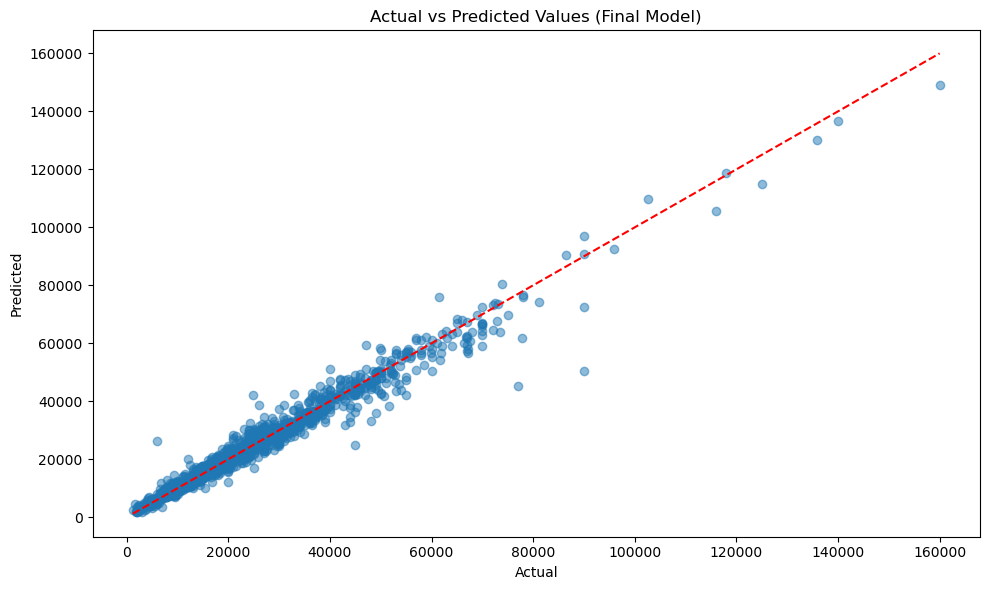
\includegraphics[keepaspectratio]{adaboost_files/figure-pdf/cell-20-output-1.png}}

\subsection{Using Optuna for Hyperparameter
Tuning}\label{using-optuna-for-hyperparameter-tuning}

\begin{Shaded}
\begin{Highlighting}[]
\NormalTok{pip install optuna}
\end{Highlighting}
\end{Shaded}

\begin{verbatim}
Collecting optuna
  Downloading optuna-4.3.0-py3-none-any.whl.metadata (17 kB)
Collecting alembic>=1.5.0 (from optuna)
  Downloading alembic-1.15.2-py3-none-any.whl.metadata (7.3 kB)
Collecting colorlog (from optuna)
  Downloading colorlog-6.9.0-py3-none-any.whl.metadata (10 kB)
Requirement already satisfied: numpy in c:\users\lsi8012\appdata\local\anaconda3\lib\site-packages (from optuna) (1.26.4)
Requirement already satisfied: packaging>=20.0 in c:\users\lsi8012\appdata\roaming\python\python312\site-packages (from optuna) (24.2)
Requirement already satisfied: sqlalchemy>=1.4.2 in c:\users\lsi8012\appdata\local\anaconda3\lib\site-packages (from optuna) (2.0.30)
Requirement already satisfied: tqdm in c:\users\lsi8012\appdata\local\anaconda3\lib\site-packages (from optuna) (4.66.4)
Requirement already satisfied: PyYAML in c:\users\lsi8012\appdata\local\anaconda3\lib\site-packages (from optuna) (6.0.1)
Collecting Mako (from alembic>=1.5.0->optuna)
  Downloading mako-1.3.10-py3-none-any.whl.metadata (2.9 kB)
Collecting typing-extensions>=4.12 (from alembic>=1.5.0->optuna)
  Downloading typing_extensions-4.13.2-py3-none-any.whl.metadata (3.0 kB)
Requirement already satisfied: greenlet!=0.4.17 in c:\users\lsi8012\appdata\local\anaconda3\lib\site-packages (from sqlalchemy>=1.4.2->optuna) (3.0.1)
Requirement already satisfied: colorama in c:\users\lsi8012\appdata\roaming\python\python312\site-packages (from colorlog->optuna) (0.4.6)
Requirement already satisfied: MarkupSafe>=0.9.2 in c:\users\lsi8012\appdata\local\anaconda3\lib\site-packages (from Mako->alembic>=1.5.0->optuna) (2.1.3)
Downloading optuna-4.3.0-py3-none-any.whl (386 kB)
   ---------------------------------------- 0.0/386.6 kB ? eta -:--:--
   ------------------ --------------------- 174.1/386.6 kB 3.5 MB/s eta 0:00:01
   ---------------------------------------- 386.6/386.6 kB 4.8 MB/s eta 0:00:00
Downloading alembic-1.15.2-py3-none-any.whl (231 kB)
   ---------------------------------------- 0.0/231.9 kB ? eta -:--:--
   ---------------------------------------- 231.9/231.9 kB 7.2 MB/s eta 0:00:00
Downloading colorlog-6.9.0-py3-none-any.whl (11 kB)
Downloading typing_extensions-4.13.2-py3-none-any.whl (45 kB)
   ---------------------------------------- 0.0/45.8 kB ? eta -:--:--
   ---------------------------------------- 45.8/45.8 kB 2.4 MB/s eta 0:00:00
Downloading mako-1.3.10-py3-none-any.whl (78 kB)
   ---------------------------------------- 0.0/78.5 kB ? eta -:--:--
   ---------------------------------------- 78.5/78.5 kB 4.6 MB/s eta 0:00:00
Installing collected packages: typing-extensions, Mako, colorlog, alembic, optuna
  Attempting uninstall: typing-extensions
    Found existing installation: typing_extensions 4.11.0
    Uninstalling typing_extensions-4.11.0:
      Successfully uninstalled typing_extensions-4.11.0
Successfully installed Mako-1.3.10 alembic-1.15.2 colorlog-6.9.0 optuna-4.3.0 typing-extensions-4.13.2
Note: you may need to restart the kernel to use updated packages.
\end{verbatim}

\begin{verbatim}
ERROR: pip's dependency resolver does not currently take into account all the packages that are installed. This behaviour is the source of the following dependency conflicts.
streamlit 1.32.0 requires packaging<24,>=16.8, but you have packaging 24.2 which is incompatible.
\end{verbatim}

Step 1: Import

\begin{Shaded}
\begin{Highlighting}[]
\CommentTok{\# import optuna}
\ImportTok{import}\NormalTok{ optuna}
\end{Highlighting}
\end{Shaded}

Step 2: Define the Objective Function

\begin{Shaded}
\begin{Highlighting}[]
\KeywordTok{def}\NormalTok{ objective(trial):}
    \CommentTok{\# Suggest hyperparameters}
\NormalTok{    learning\_rate }\OperatorTok{=}\NormalTok{ trial.suggest\_float(}\StringTok{"learning\_rate"}\NormalTok{, }\FloatTok{0.01}\NormalTok{, }\FloatTok{2.0}\NormalTok{)}
\NormalTok{    max\_depth }\OperatorTok{=}\NormalTok{ trial.suggest\_int(}\StringTok{"max\_depth"}\NormalTok{, }\DecValTok{5}\NormalTok{, }\DecValTok{25}\NormalTok{)}
\NormalTok{    n\_estimators }\OperatorTok{=}\NormalTok{ trial.suggest\_int(}\StringTok{"n\_estimators"}\NormalTok{, }\DecValTok{100}\NormalTok{, }\DecValTok{500}\NormalTok{)}

    \CommentTok{\# Define model with trial parameters}
\NormalTok{    base\_estimator }\OperatorTok{=}\NormalTok{ DecisionTreeRegressor(max\_depth}\OperatorTok{=}\NormalTok{max\_depth)}
\NormalTok{    model }\OperatorTok{=}\NormalTok{ AdaBoostRegressor(}
\NormalTok{        estimator}\OperatorTok{=}\NormalTok{base\_estimator,}
\NormalTok{        learning\_rate}\OperatorTok{=}\NormalTok{learning\_rate,}
\NormalTok{        n\_estimators}\OperatorTok{=}\NormalTok{n\_estimators,}
\NormalTok{        random\_state}\OperatorTok{=}\DecValTok{42}
\NormalTok{    )}

    \CommentTok{\# Cross{-}validation score (negative RMSE)}
\NormalTok{    score }\OperatorTok{=}\NormalTok{ cross\_val\_score(model, X\_train\_final, y\_train, scoring}\OperatorTok{=}\StringTok{"neg\_root\_mean\_squared\_error"}\NormalTok{, cv}\OperatorTok{=}\DecValTok{5}\NormalTok{)}
    \ControlFlowTok{return} \OperatorTok{{-}}\NormalTok{np.mean(score)}
\end{Highlighting}
\end{Shaded}

Step 3: Run the study

\begin{Shaded}
\begin{Highlighting}[]
\NormalTok{study }\OperatorTok{=}\NormalTok{ optuna.create\_study(direction}\OperatorTok{=}\StringTok{"minimize"}\NormalTok{)}
\NormalTok{study.optimize(objective, n\_trials}\OperatorTok{=}\DecValTok{20}\NormalTok{, timeout}\OperatorTok{=}\DecValTok{600}\NormalTok{)  }\CommentTok{\# 50 trials or 10 min}
\end{Highlighting}
\end{Shaded}

\begin{verbatim}
[I 2025-04-29 18:13:37,366] A new study created in memory with name: no-name-8c1fd49f-a877-442b-99b1-047e129cf2d6
[I 2025-04-29 18:13:55,695] Trial 0 finished with value: 3604.108244895723 and parameters: {'learning_rate': 0.2657114590825371, 'max_depth': 16, 'n_estimators': 118}. Best is trial 0 with value: 3604.108244895723.
[I 2025-04-29 18:14:39,369] Trial 1 finished with value: 3418.989299711666 and parameters: {'learning_rate': 1.3034198280227978, 'max_depth': 19, 'n_estimators': 299}. Best is trial 1 with value: 3418.989299711666.
[I 2025-04-29 18:15:01,876] Trial 2 finished with value: 6675.343723783454 and parameters: {'learning_rate': 1.8424651045294824, 'max_depth': 19, 'n_estimators': 422}. Best is trial 1 with value: 3418.989299711666.
[I 2025-04-29 18:15:51,382] Trial 3 finished with value: 3534.3761450527854 and parameters: {'learning_rate': 0.5334103211344221, 'max_depth': 12, 'n_estimators': 454}. Best is trial 1 with value: 3418.989299711666.
[I 2025-04-29 18:16:17,255] Trial 4 finished with value: 4146.601971284103 and parameters: {'learning_rate': 0.3024670447553495, 'max_depth': 8, 'n_estimators': 291}. Best is trial 1 with value: 3418.989299711666.
[I 2025-04-29 18:16:51,329] Trial 5 finished with value: 3373.6473210617305 and parameters: {'learning_rate': 1.5257826326174242, 'max_depth': 16, 'n_estimators': 256}. Best is trial 5 with value: 3373.6473210617305.
[I 2025-04-29 18:17:22,661] Trial 6 finished with value: 4645.349739417665 and parameters: {'learning_rate': 0.5297828519634237, 'max_depth': 7, 'n_estimators': 367}. Best is trial 5 with value: 3373.6473210617305.
[I 2025-04-29 18:17:48,173] Trial 7 finished with value: 3783.098791065398 and parameters: {'learning_rate': 1.4149558081471842, 'max_depth': 10, 'n_estimators': 263}. Best is trial 5 with value: 3373.6473210617305.
[I 2025-04-29 18:18:07,203] Trial 8 finished with value: 3642.6233815254373 and parameters: {'learning_rate': 1.9601482801398697, 'max_depth': 11, 'n_estimators': 188}. Best is trial 5 with value: 3373.6473210617305.
[I 2025-04-29 18:19:28,631] Trial 9 finished with value: 3815.355472103091 and parameters: {'learning_rate': 0.259029718590615, 'max_depth': 25, 'n_estimators': 452}. Best is trial 5 with value: 3373.6473210617305.
[I 2025-04-29 18:19:52,259] Trial 10 finished with value: 3460.264767659689 and parameters: {'learning_rate': 1.0867872885809007, 'max_depth': 23, 'n_estimators': 145}. Best is trial 5 with value: 3373.6473210617305.
[I 2025-04-29 18:20:24,557] Trial 11 finished with value: 3354.0174995460206 and parameters: {'learning_rate': 1.4283231452601248, 'max_depth': 17, 'n_estimators': 232}. Best is trial 11 with value: 3354.0174995460206.
[I 2025-04-29 18:20:51,602] Trial 12 finished with value: 3424.5702876072514 and parameters: {'learning_rate': 1.5895892175714832, 'max_depth': 15, 'n_estimators': 217}. Best is trial 11 with value: 3354.0174995460206.
[I 2025-04-29 18:21:42,335] Trial 13 finished with value: 3428.9633976083956 and parameters: {'learning_rate': 0.9643138493113337, 'max_depth': 17, 'n_estimators': 364}. Best is trial 11 with value: 3354.0174995460206.
[I 2025-04-29 18:22:07,861] Trial 14 finished with value: 3363.7031695680153 and parameters: {'learning_rate': 1.62982211920311, 'max_depth': 20, 'n_estimators': 234}. Best is trial 11 with value: 3354.0174995460206.
[I 2025-04-29 18:22:38,820] Trial 15 finished with value: 3467.0742139036493 and parameters: {'learning_rate': 1.0494403165070592, 'max_depth': 21, 'n_estimators': 195}. Best is trial 11 with value: 3354.0174995460206.
[I 2025-04-29 18:23:03,761] Trial 16 finished with value: 4339.523251732014 and parameters: {'learning_rate': 1.7528718262914982, 'max_depth': 21, 'n_estimators': 347}. Best is trial 11 with value: 3354.0174995460206.
[I 2025-04-29 18:23:32,216] Trial 17 finished with value: 3429.3383627414196 and parameters: {'learning_rate': 1.2930834352035752, 'max_depth': 14, 'n_estimators': 235}. Best is trial 11 with value: 3354.0174995460206.
[I 2025-04-29 18:23:46,880] Trial 18 finished with value: 3432.187531277779 and parameters: {'learning_rate': 1.6679028063369739, 'max_depth': 19, 'n_estimators': 145}. Best is trial 11 with value: 3354.0174995460206.
\end{verbatim}

Step 4: Review Best Result

\begin{Shaded}
\begin{Highlighting}[]
\BuiltInTok{print}\NormalTok{(}\StringTok{"Best RMSE:"}\NormalTok{, study.best\_value)}
\BuiltInTok{print}\NormalTok{(}\StringTok{"Best hyperparameters:"}\NormalTok{, study.best\_params)}
\end{Highlighting}
\end{Shaded}

\begin{verbatim}
Best RMSE: 3354.0174995460206
Best hyperparameters: {'learning_rate': 1.4283231452601248, 'max_depth': 17, 'n_estimators': 232}
\end{verbatim}

\begin{Shaded}
\begin{Highlighting}[]
\CommentTok{\# make a prediction using the best hyperparameters}
\NormalTok{best\_params }\OperatorTok{=}\NormalTok{ study.best\_params}
\NormalTok{base\_estimator }\OperatorTok{=}\NormalTok{ DecisionTreeRegressor(max\_depth}\OperatorTok{=}\NormalTok{best\_params[}\StringTok{\textquotesingle{}max\_depth\textquotesingle{}}\NormalTok{])}
\NormalTok{model }\OperatorTok{=}\NormalTok{ AdaBoostRegressor(}
\NormalTok{    estimator}\OperatorTok{=}\NormalTok{base\_estimator,}
\NormalTok{    learning\_rate}\OperatorTok{=}\NormalTok{best\_params[}\StringTok{\textquotesingle{}learning\_rate\textquotesingle{}}\NormalTok{],}
\NormalTok{    n\_estimators}\OperatorTok{=}\NormalTok{best\_params[}\StringTok{\textquotesingle{}n\_estimators\textquotesingle{}}\NormalTok{],}
\NormalTok{    random\_state}\OperatorTok{=}\DecValTok{42}
\NormalTok{)}
\CommentTok{\# fit the model}
\NormalTok{model.fit(X\_train\_final, y\_train)}
\CommentTok{\# predict the test set}
\NormalTok{y\_pred }\OperatorTok{=}\NormalTok{ model.predict(X\_test\_final)}
\CommentTok{\# calculate the mean squared error}
\NormalTok{rmse }\OperatorTok{=}\NormalTok{ root\_mean\_squared\_error(y\_test, y\_pred)}
\BuiltInTok{print}\NormalTok{(}\SpecialStringTok{f\textquotesingle{}RMSE: }\SpecialCharTok{\{}\NormalTok{rmse}\SpecialCharTok{:.2f\}}\SpecialStringTok{\textquotesingle{}}\NormalTok{)}
\BuiltInTok{print}\NormalTok{(}\SpecialStringTok{f\textquotesingle{}R2 Score: }\SpecialCharTok{\{}\NormalTok{r2\_score(y\_test, y\_pred)}\SpecialCharTok{\}}\SpecialStringTok{\textquotesingle{}}\NormalTok{)}
\end{Highlighting}
\end{Shaded}

\begin{verbatim}
RMSE: 3524.38
R2 Score: 0.9576611696103872
\end{verbatim}

Step 5: Visualize the Search

\begin{Shaded}
\begin{Highlighting}[]
\NormalTok{optuna.visualization.plot\_optimization\_history(study).show()}
\end{Highlighting}
\end{Shaded}

\begin{verbatim}
Unable to display output for mime type(s): application/vnd.plotly.v1+json
\end{verbatim}

\begin{Shaded}
\begin{Highlighting}[]
\NormalTok{optuna.visualization.plot\_param\_importances(study).show()}
\end{Highlighting}
\end{Shaded}

\begin{verbatim}
Unable to display output for mime type(s): application/vnd.plotly.v1+json
\end{verbatim}

\begin{Shaded}
\begin{Highlighting}[]
\NormalTok{optuna.visualization.plot\_parallel\_coordinate(study).show()}
\end{Highlighting}
\end{Shaded}

\begin{verbatim}
Unable to display output for mime type(s): application/vnd.plotly.v1+json
\end{verbatim}

\textbf{Insights:}

\begin{itemize}
\item
  Best Hyperparameter Region:

  \begin{itemize}
  \tightlist
  \item
    \texttt{learning\_rate}: \textasciitilde0.2--0.5
  \item
    \texttt{max\_depth}: \textasciitilde7--10
  \item
    \texttt{n\_estimators}: \textasciitilde300--450
  \end{itemize}
\item
  Trade-offs:

  \begin{itemize}
  \tightlist
  \item
    Increasing \texttt{n\_estimators} improves performance but increases
    computation time.
  \item
    Lower \texttt{learning\_rate} values require more estimators to
    achieve good performance.
  \end{itemize}
\item
  Next Steps:

  \begin{itemize}
  \tightlist
  \item
    Focus on fine-tuning within the identified ranges for
    \texttt{learning\_rate}, \texttt{max\_depth}, and
    \texttt{n\_estimators}.
  \item
    Use these insights to narrow the search space for further
    optimization.
  \end{itemize}
\end{itemize}

\chapter{Gradient Boosting}\label{gradient-boosting}

\emph{Note that in this course, lecture notes are not sufficient, you
must read the book for better understanding. Lecture notes are just
implementing the concepts of the book on a dataset, but not explaining
the concepts elaborately.}

\section{What is Gradient Boosting?}\label{what-is-gradient-boosting}

Gradient Boosting is a \textbf{boosting technique} that builds an
additive model in a forward stage-wise manner. Unlike AdaBoost, which
adjusts weights on training instances, Gradient Boosting fits new models
to the \textbf{residual errors} made by prior models using the gradient
of a specified loss function.

At each stage, a new weak learner is trained to minimize the loss
function by correcting the errors of the current ensemble.

\section{Gradient Boosting Intuition}\label{gradient-boosting-intuition}

Gradient Boosting can be understood as \textbf{functional gradient
descent}:

\begin{itemize}
\tightlist
\item
  We start with an initial prediction (e.g., the mean of the targets).
\item
  At each iteration, we fit a new model to the \textbf{negative
  gradient} of the loss function with respect to the current
  predictions.
\item
  This negative gradient plays a similar role to residuals in squared
  loss regression---it points in the direction that most reduces the
  loss.
\item
  The new model's predictions are then added to the current model,
  scaled by a learning rate.
\end{itemize}

By sequentially adding models that reduce the remaining error, the
ensemble gradually improves.

\section{How Gradient Boosting Works (Regression
Example)}\label{how-gradient-boosting-works-regression-example}

\begin{enumerate}
\def\labelenumi{\arabic{enumi}.}
\item
  \textbf{Initialize} the model with a constant prediction:\\
  \[
  \hat{f}^{(0)}(x) = \arg\min_c \sum_{i=1}^n L(y_i, c)
  \]
\item
  \textbf{For} \(m = 1\) to \(M\) (number of boosting rounds):

  \begin{itemize}
  \item
    Compute the \textbf{negative gradient} (pseudo-residuals):\\
    \[
    r_i^{(m)} = - \left[ \frac{\partial L(y_i, \hat{f}(x_i))}{\partial \hat{f}(x_i)} \right]_{\hat{f}(x) = \hat{f}^{(m-1)}(x)}
    \]
  \item
    Fit a \textbf{base learner} \(h^{(m)}(x)\) to the residuals
    \(r_i^{(m)}\).
  \item
    Determine the \textbf{optimal step size} (line search):\\
    \[
    \gamma^{(m)} = \arg\min_\gamma \sum_{i=1}^n L\left(y_i, \hat{f}^{(m-1)}(x_i) + \gamma \cdot h^{(m)}(x_i)\right)
    \]
  \item
    \textbf{Update the model}:\\
    \[
    \hat{f}^{(m)}(x) = \hat{f}^{(m-1)}(x) + \eta \cdot \gamma^{(m)} h^{(m)}(x)
    \] where \(\eta\) is the learning rate.
  \end{itemize}
\item
  \textbf{Final prediction}:\\
  \[
  \hat{f}^{(M)}(x)
  \]
\end{enumerate}

\begin{Shaded}
\begin{Highlighting}[]
\ImportTok{import}\NormalTok{ pandas }\ImportTok{as}\NormalTok{ pd}
\ImportTok{import}\NormalTok{ numpy }\ImportTok{as}\NormalTok{ np}
\ImportTok{import}\NormalTok{ seaborn }\ImportTok{as}\NormalTok{ sns}
\ImportTok{import}\NormalTok{ matplotlib.pyplot }\ImportTok{as}\NormalTok{ plt}
\ImportTok{from}\NormalTok{ sklearn.metrics }\ImportTok{import}\NormalTok{ mean\_squared\_error}
\ImportTok{from}\NormalTok{ sklearn.model\_selection }\ImportTok{import}\NormalTok{ cross\_val\_score,train\_test\_split, KFold, cross\_val\_predict}
\ImportTok{from}\NormalTok{ sklearn.metrics }\ImportTok{import}\NormalTok{ root\_mean\_squared\_error, mean\_squared\_error,r2\_score,roc\_curve,auc,precision\_recall\_curve, accuracy\_score, }\OperatorTok{\textbackslash{}}
\NormalTok{recall\_score, precision\_score, confusion\_matrix}
\ImportTok{from}\NormalTok{ sklearn.tree }\ImportTok{import}\NormalTok{ DecisionTreeRegressor,DecisionTreeClassifier}
\ImportTok{from}\NormalTok{ sklearn.model\_selection }\ImportTok{import}\NormalTok{ GridSearchCV, ParameterGrid, StratifiedKFold}
\ImportTok{from}\NormalTok{ sklearn.ensemble }\ImportTok{import}\NormalTok{ GradientBoostingRegressor,GradientBoostingClassifier, BaggingRegressor,BaggingClassifier,RandomForestRegressor,RandomForestClassifier,AdaBoostRegressor,AdaBoostClassifier}
\ImportTok{from}\NormalTok{ sklearn.preprocessing }\ImportTok{import}\NormalTok{ OneHotEncoder, FunctionTransformer}
\ImportTok{import}\NormalTok{ itertools }\ImportTok{as}\NormalTok{ it}
\ImportTok{import}\NormalTok{ time }\ImportTok{as}\NormalTok{ time}

\ImportTok{import}\NormalTok{ optuna}
\ImportTok{from}\NormalTok{ skopt }\ImportTok{import}\NormalTok{ BayesSearchCV}
\ImportTok{from}\NormalTok{ skopt.space }\ImportTok{import}\NormalTok{ Real, Categorical, Integer}
\ImportTok{from}\NormalTok{ skopt.plots }\ImportTok{import}\NormalTok{ plot\_objective, plot\_histogram, plot\_convergence}
\ImportTok{import}\NormalTok{ warnings}
\ImportTok{from}\NormalTok{ IPython }\ImportTok{import}\NormalTok{ display}
\end{Highlighting}
\end{Shaded}

\section{Gradient Boosting in
Scikit-Learn}\label{gradient-boosting-in-scikit-learn}

Scikit-learn offers a standard implementation of Gradient Boosting
through two primary estimators:

\begin{itemize}
\tightlist
\item
  \href{https://scikit-learn.org/stable/modules/generated/sklearn.ensemble.GradientBoostingClassifier.html}{\texttt{GradientBoostingClassifier}}
  for classification tasks
\item
  \href{https://scikit-learn.org/stable/modules/generated/sklearn.ensemble.GradientBoostingRegressor.html}{\texttt{GradientBoostingRegressor}}
  for regression tasks
\end{itemize}

These estimators build an additive model in a forward stage-wise
fashion, allowing for the optimization of arbitrary differentiable loss
functions. They are suitable for small to medium-sized datasets and
provide flexibility in model tuning.

For larger datasets (typically with
\texttt{n\_samples\ \textgreater{}=\ 10,000}), consider using the
histogram-based variants:

\begin{itemize}
\tightlist
\item
  \href{https://scikit-learn.org/stable/modules/generated/sklearn.ensemble.HistGradientBoostingClassifier.html}{\texttt{HistGradientBoostingClassifier}}
\item
  \href{https://scikit-learn.org/stable/modules/generated/sklearn.ensemble.HistGradientBoostingRegressor.html}{\texttt{HistGradientBoostingRegressor}}
\end{itemize}

\section{Core Hyperparameters
Categories}\label{core-hyperparameters-categories}

The primary hyperparameters for \texttt{GradientBoostingClassifier} and
\texttt{GradientBoostingRegressor} can be grouped into the following
categories:

\begin{enumerate}
\def\labelenumi{\arabic{enumi}.}
\item
  \textbf{Number of Trees} (\texttt{n\_estimators})

  \begin{itemize}
  \tightlist
  \item
    Use \textbf{early stopping} (via \texttt{n\_iter\_no\_change} and
    \texttt{validation\_fraction} in scikit-learn) to avoid
    overfitting.\\
  \item
    Start with a large value (e.g., 500--1000) and let early stopping
    prune unnecessary trees.
  \end{itemize}
\item
  \textbf{Early Stopping}

  \begin{itemize}
  \tightlist
  \item
    Prevents overfitting by halting training once the validation
    performance stops improving.\\
  \item
    Controlled using:

    \begin{itemize}
    \tightlist
    \item
      \texttt{n\_iter\_no\_change}: Number of rounds with no improvement
      before stopping (e.g., 10).
    \item
      \texttt{validation\_fraction}: Fraction of training data reserved
      as internal validation set (e.g., 0.1).
    \item
      \texttt{tol}: Minimum improvement to be considered significant
      (e.g., \texttt{1e-4}).
    \end{itemize}
  \item
    Set a large \texttt{n\_estimators}, and let early stopping determine
    the optimal number of boosting iterations.
  \end{itemize}
\item
  \textbf{Learning Rate} (\texttt{learning\_rate})

  \begin{itemize}
  \tightlist
  \item
    Shrinks the contribution of each tree to improve generalization.\\
  \item
    \emph{Typical range}: 0.01--0.2 (lower values require more trees).
  \end{itemize}
\item
  \textbf{Tree Complexity}

  \begin{itemize}
  \tightlist
  \item
    \texttt{max\_depth}: Depth of individual trees. Start shallow (3--6)
    to limit overfitting.\\
  \item
    \texttt{min\_samples\_split}: Minimum samples required to split a
    node (e.g., 10--50).\\
  \item
    \texttt{min\_samples\_leaf}: Minimum samples required in a leaf node
    (e.g., 5--20).
  \end{itemize}
\item
  \textbf{Stochastic Gradient Boosting}

  \begin{itemize}
  \tightlist
  \item
    \texttt{subsample}: Fraction of training data sampled per tree
    (e.g., 0.5--1.0).\\
  \item
    \texttt{max\_features}: Fraction/absolute number of features used
    per split (e.g., \texttt{sqrt(n\_features)} or \texttt{0.8}).
  \end{itemize}
\item
  \textbf{Loss Function} (\texttt{loss})

  \begin{itemize}
  \tightlist
  \item
    Matches the problem type:

    \begin{itemize}
    \tightlist
    \item
      Regression: \texttt{squared\_error}, \texttt{absolute\_error}
    \item
      Classification: \texttt{log\_loss} (binary/multinomial deviance)
    \end{itemize}
  \end{itemize}
\end{enumerate}

For a comprehensive list and detailed explanations of all
hyperparameters, refer to the official Scikit-learn documentation:

\begin{itemize}
\tightlist
\item
  \href{https://scikit-learn.org/stable/modules/generated/sklearn.ensemble.GradientBoostingClassifier.html}{GradientBoostingClassifier
  Documentation}
\item
  \href{https://scikit-learn.org/stable/modules/generated/sklearn.ensemble.GradientBoostingRegressor.html}{GradientBoostingRegressor
  Documentation}
\end{itemize}

\section{Hyperparameter Tuning}\label{hyperparameter-tuning-2}

Let's reuse the car dataset to evaluate how different hyperparameter
settings affect the performance of gradient boosting

\begin{Shaded}
\begin{Highlighting}[]
\CommentTok{\# Load the dataset}
\NormalTok{car }\OperatorTok{=}\NormalTok{ pd.read\_csv(}\StringTok{\textquotesingle{}Datasets/car.csv\textquotesingle{}}\NormalTok{)}
\NormalTok{car.head()}
\end{Highlighting}
\end{Shaded}

\begin{longtable}[]{@{}lllllllllll@{}}
\toprule\noalign{}
& brand & model & year & transmission & mileage & fuelType & tax & mpg &
engineSize & price \\
\midrule\noalign{}
\endhead
\bottomrule\noalign{}
\endlastfoot
0 & vw & Beetle & 2014 & Manual & 55457 & Diesel & 30 & 65.3266 & 1.6 &
7490 \\
1 & vauxhall & GTC & 2017 & Manual & 15630 & Petrol & 145 & 47.2049 &
1.4 & 10998 \\
2 & merc & G Class & 2012 & Automatic & 43000 & Diesel & 570 & 25.1172 &
3.0 & 44990 \\
3 & audi & RS5 & 2019 & Automatic & 10 & Petrol & 145 & 30.5593 & 2.9 &
51990 \\
4 & merc & X-CLASS & 2018 & Automatic & 14000 & Diesel & 240 & 35.7168 &
2.3 & 28990 \\
\end{longtable}

\begin{Shaded}
\begin{Highlighting}[]
\NormalTok{X }\OperatorTok{=}\NormalTok{ car.drop(columns}\OperatorTok{=}\NormalTok{[}\StringTok{\textquotesingle{}price\textquotesingle{}}\NormalTok{])}
\NormalTok{y }\OperatorTok{=}\NormalTok{ car[}\StringTok{\textquotesingle{}price\textquotesingle{}}\NormalTok{]}

\NormalTok{X\_train, X\_test, y\_train, y\_test }\OperatorTok{=}\NormalTok{ train\_test\_split(X, y, test\_size}\OperatorTok{=}\FloatTok{0.2}\NormalTok{, random\_state}\OperatorTok{=}\DecValTok{42}\NormalTok{)}

\CommentTok{\# extract the categorical columns and put them in a list}
\NormalTok{categorical\_feature }\OperatorTok{=}\NormalTok{ X.select\_dtypes(include}\OperatorTok{=}\NormalTok{[}\StringTok{\textquotesingle{}object\textquotesingle{}}\NormalTok{]).columns.tolist()}

\CommentTok{\# extract the numerical columns and put them in a list}
\NormalTok{numerical\_feature }\OperatorTok{=}\NormalTok{ X.select\_dtypes(include}\OperatorTok{=}\NormalTok{[}\StringTok{\textquotesingle{}int64\textquotesingle{}}\NormalTok{, }\StringTok{\textquotesingle{}float64\textquotesingle{}}\NormalTok{]).columns.tolist()}
\end{Highlighting}
\end{Shaded}

\begin{Shaded}
\begin{Highlighting}[]
\NormalTok{encoder }\OperatorTok{=}\NormalTok{ OneHotEncoder(handle\_unknown}\OperatorTok{=}\StringTok{\textquotesingle{}ignore\textquotesingle{}}\NormalTok{, sparse\_output}\OperatorTok{=}\VariableTok{False}\NormalTok{)}

\NormalTok{X\_train\_encoded }\OperatorTok{=}\NormalTok{ encoder.fit\_transform(X\_train[categorical\_feature])}
\NormalTok{X\_test\_encoded }\OperatorTok{=}\NormalTok{ encoder.transform(X\_test[categorical\_feature])}

\CommentTok{\# Convert the encoded features back to DataFrame}
\NormalTok{X\_train\_encoded\_df }\OperatorTok{=}\NormalTok{ pd.DataFrame(X\_train\_encoded, columns}\OperatorTok{=}\NormalTok{encoder.get\_feature\_names\_out(categorical\_feature))}
\NormalTok{X\_test\_encoded\_df }\OperatorTok{=}\NormalTok{ pd.DataFrame(X\_test\_encoded, columns}\OperatorTok{=}\NormalTok{encoder.get\_feature\_names\_out(categorical\_feature))}

\CommentTok{\# Concatenate the encoded features with the original numerical features}
\NormalTok{X\_train\_final }\OperatorTok{=}\NormalTok{ pd.concat([X\_train\_encoded\_df, X\_train[numerical\_feature].reset\_index(drop}\OperatorTok{=}\VariableTok{True}\NormalTok{)], axis}\OperatorTok{=}\DecValTok{1}\NormalTok{)}
\NormalTok{X\_test\_final }\OperatorTok{=}\NormalTok{ pd.concat([X\_test\_encoded\_df, X\_test[numerical\_feature].reset\_index(drop}\OperatorTok{=}\VariableTok{True}\NormalTok{)], axis}\OperatorTok{=}\DecValTok{1}\NormalTok{)}
\end{Highlighting}
\end{Shaded}

\subsection{Individual Hyperparameter Impact
Analysis}\label{individual-hyperparameter-impact-analysis}

\subsubsection{Effect of Number of Trees on Cross-Validation
Error}\label{effect-of-number-of-trees-on-cross-validation-error}

Effect of Number of Trees on Cross-Validation Error In Gradient
Boosting, the number of trees (\texttt{n\_estimators}) controls how many
boosting rounds the model performs. Adding more trees can reduce bias
and improve training accuracy, but it also increases the risk of
overfitting, especially with a high learning rate.

The optimal number of trees is often found by balancing \textbf{model
complexity} and \textbf{generalization performance} using
cross-validation.

\begin{Shaded}
\begin{Highlighting}[]
\KeywordTok{def}\NormalTok{ get\_models():}
\NormalTok{    models }\OperatorTok{=} \BuiltInTok{dict}\NormalTok{()}
    \CommentTok{\# define number of trees to consider}
\NormalTok{    n\_trees }\OperatorTok{=}\NormalTok{ [}\DecValTok{50}\NormalTok{, }\DecValTok{100}\NormalTok{, }\DecValTok{500}\NormalTok{, }\DecValTok{800}\NormalTok{, }\DecValTok{1000}\NormalTok{, }\DecValTok{1500}\NormalTok{, }\DecValTok{2000}\NormalTok{]}
    \ControlFlowTok{for}\NormalTok{ n }\KeywordTok{in}\NormalTok{ n\_trees:}
\NormalTok{        models[}\BuiltInTok{str}\NormalTok{(n)] }\OperatorTok{=}\NormalTok{ GradientBoostingRegressor(n\_estimators}\OperatorTok{=}\NormalTok{n,random\_state}\OperatorTok{=}\DecValTok{1}\NormalTok{,loss}\OperatorTok{=}\StringTok{\textquotesingle{}huber\textquotesingle{}}\NormalTok{)}
    \ControlFlowTok{return}\NormalTok{ models}

\CommentTok{\# evaluate a given model using cross{-}validation}
\KeywordTok{def}\NormalTok{ evaluate\_model(model, X, y):}
    \CommentTok{\# define the evaluation procedure}
\NormalTok{    cv }\OperatorTok{=}\NormalTok{ KFold(n\_splits}\OperatorTok{=}\DecValTok{5}\NormalTok{, shuffle}\OperatorTok{=}\VariableTok{True}\NormalTok{, random\_state}\OperatorTok{=}\DecValTok{1}\NormalTok{)}
    \CommentTok{\# evaluate the model and collect the results}
\NormalTok{    scores }\OperatorTok{=}\NormalTok{ np.sqrt(}\OperatorTok{{-}}\NormalTok{cross\_val\_score(model, X, y, scoring}\OperatorTok{=}\StringTok{\textquotesingle{}neg\_mean\_squared\_error\textquotesingle{}}\NormalTok{, cv}\OperatorTok{=}\NormalTok{cv, n\_jobs}\OperatorTok{={-}}\DecValTok{1}\NormalTok{))}
    \ControlFlowTok{return}\NormalTok{ scores}

\CommentTok{\# get the models to evaluate}
\NormalTok{models }\OperatorTok{=}\NormalTok{ get\_models()}
\CommentTok{\# evaluate the models and store results}
\NormalTok{results, names }\OperatorTok{=} \BuiltInTok{list}\NormalTok{(), }\BuiltInTok{list}\NormalTok{()}
\ControlFlowTok{for}\NormalTok{ name, model }\KeywordTok{in}\NormalTok{ models.items():}
    \CommentTok{\# evaluate the model}
\NormalTok{    scores }\OperatorTok{=}\NormalTok{ evaluate\_model(model, X\_train\_final, y\_train)}
    \CommentTok{\# store the results}
\NormalTok{    results.append(scores)}
\NormalTok{    names.append(name)}
    \CommentTok{\# summarize the performance along the way}
    \BuiltInTok{print}\NormalTok{(}\StringTok{\textquotesingle{}\textgreater{}}\SpecialCharTok{\%s}\StringTok{ }\SpecialCharTok{\%.3f}\StringTok{ (}\SpecialCharTok{\%.3f}\StringTok{)\textquotesingle{}} \OperatorTok{\%}\NormalTok{ (name, np.mean(scores), np.std(scores)))}

\NormalTok{plt.boxplot(results, labels}\OperatorTok{=}\NormalTok{names, showmeans}\OperatorTok{=}\VariableTok{True}\NormalTok{)}
\NormalTok{plt.ylabel(}\StringTok{\textquotesingle{}Cross validation error\textquotesingle{}}\NormalTok{,fontsize}\OperatorTok{=}\DecValTok{15}\NormalTok{)}
\NormalTok{plt.xlabel(}\StringTok{\textquotesingle{}Number of trees\textquotesingle{}}\NormalTok{,fontsize}\OperatorTok{=}\DecValTok{15}\NormalTok{)}\OperatorTok{;}

\CommentTok{\# get the optimal number of trees}
\NormalTok{best\_index }\OperatorTok{=}\NormalTok{ np.argmin([np.mean(r) }\ControlFlowTok{for}\NormalTok{ r }\KeywordTok{in}\NormalTok{ results])}
\NormalTok{best\_n\_trees }\OperatorTok{=}\NormalTok{ names[best\_index]}
\NormalTok{best\_score }\OperatorTok{=}\NormalTok{ np.mean(results[best\_index])}


\CommentTok{\# Highlight the best model on the plot}
\NormalTok{plt.axvline(x}\OperatorTok{=}\NormalTok{best\_index}\OperatorTok{+}\DecValTok{1}\NormalTok{, color}\OperatorTok{=}\StringTok{\textquotesingle{}red\textquotesingle{}}\NormalTok{, linestyle}\OperatorTok{=}\StringTok{\textquotesingle{}{-}{-}\textquotesingle{}}\NormalTok{, alpha}\OperatorTok{=}\FloatTok{0.7}\NormalTok{)}
\NormalTok{plt.text(best\_index }\OperatorTok{+} \DecValTok{1} \OperatorTok{{-}} \FloatTok{0.4}\NormalTok{, best\_score}\OperatorTok{+}\DecValTok{700}\NormalTok{, }
         \SpecialStringTok{f\textquotesingle{}Best: }\SpecialCharTok{\{}\NormalTok{best\_n\_trees}\SpecialCharTok{\}}\SpecialStringTok{ (RMSE: }\SpecialCharTok{\{}\NormalTok{best\_score}\SpecialCharTok{:.1f\}}\SpecialStringTok{)\textquotesingle{}}\NormalTok{, }
\NormalTok{         color}\OperatorTok{=}\StringTok{\textquotesingle{}red\textquotesingle{}}\NormalTok{, fontweight}\OperatorTok{=}\StringTok{\textquotesingle{}bold\textquotesingle{}}\NormalTok{)}

\BuiltInTok{print}\NormalTok{(}\SpecialStringTok{f"Best number of trees: }\SpecialCharTok{\{}\NormalTok{best\_n\_trees}\SpecialCharTok{\}}\SpecialStringTok{ with RMSE: }\SpecialCharTok{\{}\NormalTok{best\_score}\SpecialCharTok{:.3f\}}\SpecialStringTok{"}\NormalTok{)}
\end{Highlighting}
\end{Shaded}

\begin{verbatim}
>50 6549.576 (722.462)
>100 5232.949 (656.216)
>500 3419.467 (262.753)
>800 3202.489 (194.072)
>1000 3106.002 (184.799)
>1500 3039.520 (210.989)
>2000 3194.874 (293.134)
Best number of trees: 1500 with RMSE: 3039.520
\end{verbatim}

\pandocbounded{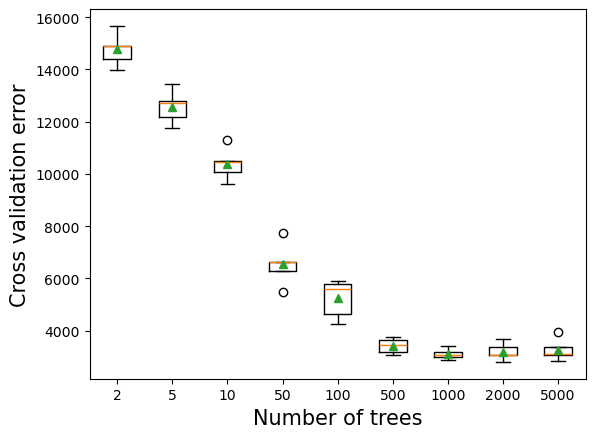
\includegraphics[keepaspectratio]{Gradient_Boosting_files/figure-pdf/cell-6-output-2.png}}

\subsubsection{Early stopping in Gradient
Boosting}\label{early-stopping-in-gradient-boosting}

\textbf{Why Early Stopping Matters}

Specifying a fixed number of trees means deciding in advance how many
boosting rounds (i.e., trees) the model will train.

This approach can be inefficient or risky:

\begin{itemize}
\tightlist
\item
  If \textbf{too few} trees are used, the model may \textbf{underfit}.
\item
  If \textbf{too many}, the model may \textbf{overfit} or \textbf{waste
  computation}.
\end{itemize}

That's why \textbf{early stopping} is useful --- it allows the model to
\textbf{stop training once performance on a validation set no longer
improves}, effectively selecting the optimal number of trees
automatically.

\textbf{How Early Stopping Works}

Instead of specifying a fixed number of trees (\texttt{n\_estimators}),
the algorithm monitors performance on a \textbf{validation set} and
stops adding new trees once the model's improvement has plateaued.

In scikit-learn, early stopping can be enabled using:

\begin{itemize}
\tightlist
\item
  \texttt{early\_stopping=True}
\item
  \texttt{validation\_fraction}: The fraction of training data used as a
  validation set
\item
  \texttt{n\_iter\_no\_change}: Number of iterations to wait without
  improvement before stopping
\end{itemize}

This approach not only improves generalization but also reduces training
time by avoiding unnecessary trees.

\begin{Shaded}
\begin{Highlighting}[]
\NormalTok{params }\OperatorTok{=} \BuiltInTok{dict}\NormalTok{(n\_estimators}\OperatorTok{=}\DecValTok{2000}\NormalTok{, max\_depth}\OperatorTok{=}\DecValTok{5}\NormalTok{, learning\_rate}\OperatorTok{=}\FloatTok{0.1}\NormalTok{, random\_state}\OperatorTok{=}\DecValTok{42}\NormalTok{)}

\NormalTok{gbm\_full }\OperatorTok{=}\NormalTok{ GradientBoostingRegressor(}\OperatorTok{**}\NormalTok{params)}
\NormalTok{gbm\_early\_stopping }\OperatorTok{=}\NormalTok{ GradientBoostingRegressor(}
    \OperatorTok{**}\NormalTok{params,}
\NormalTok{    validation\_fraction}\OperatorTok{=}\FloatTok{0.1}\NormalTok{,}
\NormalTok{    n\_iter\_no\_change}\OperatorTok{=}\DecValTok{10}\NormalTok{,}
\NormalTok{)}

\NormalTok{start\_time }\OperatorTok{=}\NormalTok{ time.time()}
\NormalTok{gbm\_full.fit(X\_train\_final, y\_train)}
\NormalTok{training\_time\_full }\OperatorTok{=}\NormalTok{ time.time() }\OperatorTok{{-}}\NormalTok{ start\_time}
\NormalTok{n\_estimators\_full }\OperatorTok{=}\NormalTok{ gbm\_full.n\_estimators\_}

\NormalTok{start\_time }\OperatorTok{=}\NormalTok{ time.time()}
\NormalTok{gbm\_early\_stopping.fit(X\_train\_final, y\_train)}
\NormalTok{training\_time\_early\_stopping }\OperatorTok{=}\NormalTok{ time.time() }\OperatorTok{{-}}\NormalTok{ start\_time}
\NormalTok{estimators\_early\_stopping }\OperatorTok{=}\NormalTok{ gbm\_early\_stopping.n\_estimators\_}
\end{Highlighting}
\end{Shaded}

Let's calculate the RMSE on both the training and test datasets for each
model, which will be used for later visualization.

\begin{Shaded}
\begin{Highlighting}[]
\CommentTok{\# import root mean squared error function}
\ImportTok{from}\NormalTok{ sklearn.metrics }\ImportTok{import}\NormalTok{ root\_mean\_squared\_error}

\NormalTok{train\_errors\_without }\OperatorTok{=}\NormalTok{ []}
\NormalTok{test\_errors\_without }\OperatorTok{=}\NormalTok{ []}

\NormalTok{train\_errors\_with }\OperatorTok{=}\NormalTok{ []}
\NormalTok{test\_errors\_with }\OperatorTok{=}\NormalTok{ []}

\ControlFlowTok{for}\NormalTok{ i, (train\_pred, test\_pred) }\KeywordTok{in} \BuiltInTok{enumerate}\NormalTok{(}
    \BuiltInTok{zip}\NormalTok{(}
\NormalTok{        gbm\_full.staged\_predict(X\_train\_final),}
\NormalTok{        gbm\_full.staged\_predict(X\_test\_final),}
\NormalTok{    )}
\NormalTok{):}
\NormalTok{    train\_errors\_without.append(root\_mean\_squared\_error(y\_train, train\_pred))}
\NormalTok{    test\_errors\_without.append(root\_mean\_squared\_error(y\_test, test\_pred))}

\ControlFlowTok{for}\NormalTok{ i, (train\_pred, test\_pred) }\KeywordTok{in} \BuiltInTok{enumerate}\NormalTok{(}
    \BuiltInTok{zip}\NormalTok{(}
\NormalTok{        gbm\_early\_stopping.staged\_predict(X\_train\_final),}
\NormalTok{        gbm\_early\_stopping.staged\_predict(X\_test\_final),}
\NormalTok{    )}
\NormalTok{):}
\NormalTok{    train\_errors\_with.append(root\_mean\_squared\_error(y\_train, train\_pred))}
\NormalTok{    test\_errors\_with.append(root\_mean\_squared\_error(y\_test, test\_pred))}
\end{Highlighting}
\end{Shaded}

Let's visulize Comparison. It includes three subplots:

\begin{enumerate}
\def\labelenumi{\arabic{enumi}.}
\tightlist
\item
  Plotting training errors of both models over boosting iterations.
\item
  Plotting test errors of both models over boosting iterations.
\item
  Creating a bar chart to compare the training times and the number of
  estimators used by the models with and without early stopping.
\end{enumerate}

\begin{Shaded}
\begin{Highlighting}[]
\NormalTok{fig, axes }\OperatorTok{=}\NormalTok{ plt.subplots(ncols}\OperatorTok{=}\DecValTok{3}\NormalTok{, figsize}\OperatorTok{=}\NormalTok{(}\DecValTok{12}\NormalTok{, }\DecValTok{4}\NormalTok{))}

\NormalTok{axes[}\DecValTok{0}\NormalTok{].plot(train\_errors\_without, label}\OperatorTok{=}\StringTok{"gbm\_full"}\NormalTok{)}
\NormalTok{axes[}\DecValTok{0}\NormalTok{].plot(train\_errors\_with, label}\OperatorTok{=}\StringTok{"gbm\_early\_stopping"}\NormalTok{)}
\NormalTok{axes[}\DecValTok{0}\NormalTok{].set\_xlabel(}\StringTok{"Boosting Iterations"}\NormalTok{)}
\NormalTok{axes[}\DecValTok{0}\NormalTok{].set\_ylabel(}\StringTok{"RMSE (Training)"}\NormalTok{)}
\NormalTok{axes[}\DecValTok{0}\NormalTok{].set\_yscale(}\StringTok{"log"}\NormalTok{)}
\NormalTok{axes[}\DecValTok{0}\NormalTok{].legend()}
\NormalTok{axes[}\DecValTok{0}\NormalTok{].set\_title(}\StringTok{"Training Error"}\NormalTok{)}

\NormalTok{axes[}\DecValTok{1}\NormalTok{].plot(test\_errors\_without, label}\OperatorTok{=}\StringTok{"gbm\_full"}\NormalTok{)}
\NormalTok{axes[}\DecValTok{1}\NormalTok{].plot(test\_errors\_with, label}\OperatorTok{=}\StringTok{"gbm\_early\_stopping"}\NormalTok{)}
\NormalTok{axes[}\DecValTok{1}\NormalTok{].set\_xlabel(}\StringTok{"Boosting Iterations"}\NormalTok{)}
\NormalTok{axes[}\DecValTok{1}\NormalTok{].set\_ylabel(}\StringTok{"RMSE (Test)"}\NormalTok{)}
\NormalTok{axes[}\DecValTok{1}\NormalTok{].set\_yscale(}\StringTok{"log"}\NormalTok{)}
\NormalTok{axes[}\DecValTok{1}\NormalTok{].legend()}
\NormalTok{axes[}\DecValTok{1}\NormalTok{].set\_title(}\StringTok{"Test Error"}\NormalTok{)}

\NormalTok{training\_times }\OperatorTok{=}\NormalTok{ [training\_time\_full, training\_time\_early\_stopping]}
\NormalTok{labels }\OperatorTok{=}\NormalTok{ [}\StringTok{"gbm\_full"}\NormalTok{, }\StringTok{"gbm\_early\_stopping"}\NormalTok{]}
\NormalTok{bars }\OperatorTok{=}\NormalTok{ axes[}\DecValTok{2}\NormalTok{].bar(labels, training\_times)}
\NormalTok{axes[}\DecValTok{2}\NormalTok{].set\_ylabel(}\StringTok{"Training Time (s)"}\NormalTok{)}

\ControlFlowTok{for}\NormalTok{ bar, n\_estimators }\KeywordTok{in} \BuiltInTok{zip}\NormalTok{(bars, [n\_estimators\_full, estimators\_early\_stopping]):}
\NormalTok{    height }\OperatorTok{=}\NormalTok{ bar.get\_height()}
\NormalTok{    axes[}\DecValTok{2}\NormalTok{].text(}
\NormalTok{        bar.get\_x() }\OperatorTok{+}\NormalTok{ bar.get\_width() }\OperatorTok{/} \DecValTok{2}\NormalTok{,}
\NormalTok{        height }\OperatorTok{+} \FloatTok{0.001}\NormalTok{,}
        \SpecialStringTok{f"Estimators: }\SpecialCharTok{\{}\NormalTok{n\_estimators}\SpecialCharTok{\}}\SpecialStringTok{"}\NormalTok{,}
\NormalTok{        ha}\OperatorTok{=}\StringTok{"center"}\NormalTok{,}
\NormalTok{        va}\OperatorTok{=}\StringTok{"bottom"}\NormalTok{,}
\NormalTok{    )}

\NormalTok{plt.tight\_layout()}
\NormalTok{plt.show()}
\end{Highlighting}
\end{Shaded}

\pandocbounded{\includegraphics[keepaspectratio]{Gradient_Boosting_files/figure-pdf/cell-9-output-1.png}}

The difference in training error between the \texttt{gbm\_full} and the
\texttt{gbm\_early\_stopping} stems from the fact that\\
\texttt{gbm\_early\_stopping} sets aside \texttt{validation\_fraction}
of the training data as an internal validation set.

Early stopping is decided based on this internal validation score.

\textbf{Benefits of Using Early Stopping in Boosting:}

\begin{itemize}
\item
  \textbf{Preventing Overfitting}\\
  Early stopping helps avoid overfitting by monitoring the test error.\\
  When the error stabilizes or starts increasing, training stops ---
  resulting in better generalization to unseen data.
\item
  \textbf{Improving Training Efficiency}\\
  Models with early stopping often require \textbf{fewer estimators}
  while achieving similar accuracy.\\
  This reduces training time significantly compared to training without
  early stopping.
\end{itemize}

\subsubsection{Effect of Learning Rate on Cross-Validation
Error}\label{effect-of-learning-rate-on-cross-validation-error}

The learning rate (\texttt{learning\_rate}) determines how much each new
tree contributes to the overall model. A \textbf{smaller learning rate}
results in slower learning and often requires more trees to achieve good
performance. A \textbf{larger learning rate} speeds up learning but
increases the risk of overfitting.

Finding the optimal learning rate involves balancing: - \textbf{High
learning rate} → faster convergence, but higher risk of overfitting\\
- \textbf{Low learning rate} → better generalization, but requires more
trees and longer training time

Cross-validation helps identify the learning rate that minimizes
prediction error while ensuring model stability.

\begin{Shaded}
\begin{Highlighting}[]
\KeywordTok{def}\NormalTok{ get\_models():}
\NormalTok{    models }\OperatorTok{=} \BuiltInTok{dict}\NormalTok{()}
    \CommentTok{\# create 9 evenly spaced values between 0.2 and 1.0}
\NormalTok{    learning\_rates }\OperatorTok{=}\NormalTok{ np.linspace(}\FloatTok{0.2}\NormalTok{, }\FloatTok{1.0}\NormalTok{, }\DecValTok{9}\NormalTok{)}
    \ControlFlowTok{for}\NormalTok{ learning\_rate }\KeywordTok{in}\NormalTok{ learning\_rates:}
        \CommentTok{\# Round to 2 decimal places for clean keys}
\NormalTok{        lr\_rounded }\OperatorTok{=} \BuiltInTok{round}\NormalTok{(learning\_rate, }\DecValTok{2}\NormalTok{)}
\NormalTok{        key }\OperatorTok{=} \SpecialStringTok{f"}\SpecialCharTok{\{}\NormalTok{lr\_rounded}\SpecialCharTok{:.2f\}}\SpecialStringTok{"}
\NormalTok{        models[key] }\OperatorTok{=}\NormalTok{ GradientBoostingRegressor(learning\_rate}\OperatorTok{=}\NormalTok{lr\_rounded, random\_state}\OperatorTok{=}\DecValTok{1}\NormalTok{, loss}\OperatorTok{=}\StringTok{\textquotesingle{}huber\textquotesingle{}}\NormalTok{)}
    \ControlFlowTok{return}\NormalTok{ models}

\CommentTok{\# evaluate a given model using cross{-}validation}
\KeywordTok{def}\NormalTok{ evaluate\_model(model, X, y):}
    \CommentTok{\# define the evaluation procedure}
\NormalTok{    cv }\OperatorTok{=}\NormalTok{ KFold(n\_splits}\OperatorTok{=}\DecValTok{5}\NormalTok{, shuffle}\OperatorTok{=}\VariableTok{True}\NormalTok{, random\_state}\OperatorTok{=}\DecValTok{1}\NormalTok{)}
    \CommentTok{\# evaluate the model and collect the results}
\NormalTok{    scores }\OperatorTok{=}\NormalTok{ np.sqrt(}\OperatorTok{{-}}\NormalTok{cross\_val\_score(model, X, y, scoring}\OperatorTok{=}\StringTok{\textquotesingle{}neg\_mean\_squared\_error\textquotesingle{}}\NormalTok{, cv}\OperatorTok{=}\NormalTok{cv, n\_jobs}\OperatorTok{={-}}\DecValTok{1}\NormalTok{))}
    \ControlFlowTok{return}\NormalTok{ scores}

\CommentTok{\# get the models to evaluate}
\NormalTok{models }\OperatorTok{=}\NormalTok{ get\_models()}

\CommentTok{\# evaluate the models and store results}
\NormalTok{results, names }\OperatorTok{=} \BuiltInTok{list}\NormalTok{(), }\BuiltInTok{list}\NormalTok{()}
\NormalTok{mean\_scores }\OperatorTok{=}\NormalTok{ []  }\CommentTok{\# Track mean scores separately}

\ControlFlowTok{for}\NormalTok{ name, model }\KeywordTok{in}\NormalTok{ models.items():}
    \CommentTok{\# evaluate the model}
\NormalTok{    scores }\OperatorTok{=}\NormalTok{ evaluate\_model(model, X\_train\_final, y\_train)}
    \CommentTok{\# store the results}
\NormalTok{    results.append(scores)}
\NormalTok{    names.append(name)}
    \CommentTok{\# Calculate and store mean score}
\NormalTok{    mean\_score }\OperatorTok{=}\NormalTok{ np.mean(scores)}
\NormalTok{    mean\_scores.append(mean\_score)}
    \CommentTok{\# summarize the performance along the way}
    \BuiltInTok{print}\NormalTok{(}\StringTok{\textquotesingle{}\textgreater{}}\SpecialCharTok{\%s}\StringTok{ }\SpecialCharTok{\%.1f}\StringTok{ (}\SpecialCharTok{\%.1f}\StringTok{)\textquotesingle{}} \OperatorTok{\%}\NormalTok{ (name, mean\_score, np.std(scores)))}

\CommentTok{\# plot model performance for comparison}
\NormalTok{plt.figure(figsize}\OperatorTok{=}\NormalTok{(}\DecValTok{10}\NormalTok{, }\DecValTok{7}\NormalTok{))}
\NormalTok{plt.boxplot(results, labels}\OperatorTok{=}\NormalTok{names, showmeans}\OperatorTok{=}\VariableTok{True}\NormalTok{)}
\NormalTok{plt.ylabel(}\StringTok{\textquotesingle{}Cross validation error\textquotesingle{}}\NormalTok{, fontsize}\OperatorTok{=}\DecValTok{15}\NormalTok{)}
\NormalTok{plt.xlabel(}\StringTok{\textquotesingle{}Learning rate\textquotesingle{}}\NormalTok{, fontsize}\OperatorTok{=}\DecValTok{15}\NormalTok{)}
\NormalTok{plt.title(}\StringTok{\textquotesingle{}Model Performance by Learning Rate\textquotesingle{}}\NormalTok{, fontsize}\OperatorTok{=}\DecValTok{16}\NormalTok{)}
\NormalTok{plt.grid(}\VariableTok{True}\NormalTok{, linestyle}\OperatorTok{=}\StringTok{\textquotesingle{}{-}{-}\textquotesingle{}}\NormalTok{, alpha}\OperatorTok{=}\FloatTok{0.7}\NormalTok{)}

\CommentTok{\# Find the best model using the saved mean scores}
\NormalTok{best\_index }\OperatorTok{=}\NormalTok{ np.argmin(mean\_scores)}
\NormalTok{best\_lr }\OperatorTok{=}\NormalTok{ names[best\_index]}
\NormalTok{best\_score }\OperatorTok{=}\NormalTok{ mean\_scores[best\_index]}

\CommentTok{\# Highlight the best model on the plot}
\NormalTok{plt.axvline(x}\OperatorTok{=}\NormalTok{best\_index}\OperatorTok{+}\DecValTok{1}\NormalTok{, color}\OperatorTok{=}\StringTok{\textquotesingle{}red\textquotesingle{}}\NormalTok{, linestyle}\OperatorTok{=}\StringTok{\textquotesingle{}{-}{-}\textquotesingle{}}\NormalTok{, alpha}\OperatorTok{=}\FloatTok{0.7}\NormalTok{)}
\NormalTok{plt.text(best\_index}\OperatorTok{+}\FloatTok{1.2}\NormalTok{, }\BuiltInTok{min}\NormalTok{(mean\_scores)}\OperatorTok{*}\FloatTok{0.95}\NormalTok{, }
         \SpecialStringTok{f\textquotesingle{}Best: }\SpecialCharTok{\{}\NormalTok{best\_lr}\SpecialCharTok{\}}\SpecialStringTok{ (RMSE: }\SpecialCharTok{\{}\NormalTok{best\_score}\SpecialCharTok{:.1f\}}\SpecialStringTok{)\textquotesingle{}}\NormalTok{, }
\NormalTok{         color}\OperatorTok{=}\StringTok{\textquotesingle{}red\textquotesingle{}}\NormalTok{, fontweight}\OperatorTok{=}\StringTok{\textquotesingle{}bold\textquotesingle{}}\NormalTok{)}

\NormalTok{plt.show()}

\CommentTok{\# Print the best model information}
\BuiltInTok{print}\NormalTok{(}\SpecialStringTok{f"}\CharTok{\textbackslash{}n}\SpecialStringTok{Best model: }\SpecialCharTok{\{}\NormalTok{best\_lr}\SpecialCharTok{\}}\SpecialStringTok{ with RMSE: }\SpecialCharTok{\{}\NormalTok{best\_score}\SpecialCharTok{:.3f\}}\SpecialStringTok{"}\NormalTok{)}
\end{Highlighting}
\end{Shaded}

\begin{verbatim}
>0.20 4193.7 (301.2)
>0.30 3740.3 (306.3)
>0.40 3630.0 (212.2)
>0.50 3529.6 (181.5)
>0.60 3650.2 (169.0)
>0.70 3644.7 (142.5)
>0.80 3908.9 (260.6)
>0.90 3968.7 (201.1)
>1.00 4208.3 (368.5)
\end{verbatim}

\pandocbounded{\includegraphics[keepaspectratio]{Gradient_Boosting_files/figure-pdf/cell-10-output-2.png}}

\begin{verbatim}

Best model: 0.50 with RMSE: 3529.563
\end{verbatim}

\subsubsection{Learning Rate and Number of Trees Are Closely
Linked}\label{learning-rate-and-number-of-trees-are-closely-linked}

The \textbf{learning rate} and \textbf{number of trees}
(\texttt{n\_estimators}) are tightly coupled hyperparameters in gradient
boosting. Their balance plays a key role in model performance and
overfitting control.

\begin{itemize}
\tightlist
\item
  A \textbf{lower learning rate} slows the learning process, requiring
  \textbf{more trees} to achieve strong performance.
\item
  A \textbf{higher learning rate} speeds up training but may cause the
  model to \textbf{overfit} if not regularized properly.
\end{itemize}

⚠️ A high learning rate with too few trees can lead to poor
generalization, while a very low learning rate with too many trees may
improve accuracy but increase training time significantly.

\textbf{Best practice:} Use a low to moderate learning rate (e.g.,
\texttt{0.01}--\texttt{0.1}) combined with \textbf{early stopping} to
find the optimal number of trees.

\subsubsection{Effect of Stochastic Gradient Boosting on
Cross-Validation
Error}\label{effect-of-stochastic-gradient-boosting-on-cross-validation-error}

\textbf{Stochastic Gradient Boosting} enhances generalization by
introducing randomness into the model-building process. Two key
hyperparameters that control this are \texttt{subsample} and
\texttt{max\_features}, and they operate on \textbf{different
dimensions} of the data:

\begin{longtable}[]{@{}
  >{\raggedright\arraybackslash}p{(\linewidth - 4\tabcolsep) * \real{0.1429}}
  >{\raggedright\arraybackslash}p{(\linewidth - 4\tabcolsep) * \real{0.2054}}
  >{\raggedright\arraybackslash}p{(\linewidth - 4\tabcolsep) * \real{0.6518}}@{}}
\toprule\noalign{}
\begin{minipage}[b]{\linewidth}\raggedright
Parameter
\end{minipage} & \begin{minipage}[b]{\linewidth}\raggedright
Applies To
\end{minipage} & \begin{minipage}[b]{\linewidth}\raggedright
Purpose
\end{minipage} \\
\midrule\noalign{}
\endhead
\bottomrule\noalign{}
\endlastfoot
\texttt{subsample} & Rows (data points) & Randomly samples a fraction of
the training data for each tree \\
\texttt{max\_features} & Columns (features) & Randomly samples a
fraction of the features for each tree or split \\
\end{longtable}

By tuning these parameters, we can reduce overfitting and increase model
robustness. However, setting them too low may lead to underfitting due
to insufficient information per tree.

\begin{Shaded}
\begin{Highlighting}[]
\ImportTok{from}\NormalTok{ sklearn.metrics }\ImportTok{import}\NormalTok{ make\_scorer, mean\_squared\_error}

\CommentTok{\# Define model}
\NormalTok{model }\OperatorTok{=}\NormalTok{ GradientBoostingRegressor(n\_estimators}\OperatorTok{=}\DecValTok{100}\NormalTok{, max\_depth}\OperatorTok{=}\DecValTok{4}\NormalTok{, learning\_rate}\OperatorTok{=}\FloatTok{0.1}\NormalTok{, random\_state}\OperatorTok{=}\DecValTok{1}\NormalTok{)}

\CommentTok{\# Define param grid}
\NormalTok{param\_grid }\OperatorTok{=}\NormalTok{ \{}
    \StringTok{\textquotesingle{}subsample\textquotesingle{}}\NormalTok{: np.linspace(}\FloatTok{0.2}\NormalTok{, }\FloatTok{1.0}\NormalTok{, }\DecValTok{9}\NormalTok{),}
    \StringTok{\textquotesingle{}max\_features\textquotesingle{}}\NormalTok{: np.linspace(}\FloatTok{0.2}\NormalTok{, }\FloatTok{1.0}\NormalTok{, }\DecValTok{9}\NormalTok{)}
\NormalTok{\}}

\CommentTok{\# RMSE scoring}
\NormalTok{scorer }\OperatorTok{=}\NormalTok{ make\_scorer(mean\_squared\_error, greater\_is\_better}\OperatorTok{=}\VariableTok{False}\NormalTok{)}

\CommentTok{\# Grid search}
\NormalTok{grid }\OperatorTok{=}\NormalTok{ GridSearchCV(estimator}\OperatorTok{=}\NormalTok{model, param\_grid}\OperatorTok{=}\NormalTok{param\_grid,}
\NormalTok{                    scoring}\OperatorTok{=}\NormalTok{scorer, cv}\OperatorTok{=}\DecValTok{5}\NormalTok{, n\_jobs}\OperatorTok{={-}}\DecValTok{1}\NormalTok{, verbose}\OperatorTok{=}\DecValTok{1}\NormalTok{)}
\NormalTok{grid.fit(X\_train\_final, y\_train)}

\CommentTok{\# Create DataFrame from results}
\NormalTok{results\_df }\OperatorTok{=}\NormalTok{ pd.DataFrame(grid.cv\_results\_)}
\NormalTok{results\_df[}\StringTok{\textquotesingle{}mean\_rmse\textquotesingle{}}\NormalTok{] }\OperatorTok{=}\NormalTok{ np.sqrt(}\OperatorTok{{-}}\NormalTok{results\_df[}\StringTok{\textquotesingle{}mean\_test\_score\textquotesingle{}}\NormalTok{])}
\end{Highlighting}
\end{Shaded}

\begin{verbatim}
Fitting 5 folds for each of 81 candidates, totalling 405 fits
\end{verbatim}

\begin{Shaded}
\begin{Highlighting}[]
\CommentTok{\# Round subsample and max\_features to 2 decimal places for display}
\NormalTok{results\_df[}\StringTok{\textquotesingle{}subsample\textquotesingle{}}\NormalTok{] }\OperatorTok{=}\NormalTok{ results\_df[}\StringTok{\textquotesingle{}param\_subsample\textquotesingle{}}\NormalTok{].astype(}\BuiltInTok{float}\NormalTok{).}\BuiltInTok{round}\NormalTok{(}\DecValTok{2}\NormalTok{)}
\NormalTok{results\_df[}\StringTok{\textquotesingle{}max\_features\textquotesingle{}}\NormalTok{] }\OperatorTok{=}\NormalTok{ results\_df[}\StringTok{\textquotesingle{}param\_max\_features\textquotesingle{}}\NormalTok{].astype(}\BuiltInTok{float}\NormalTok{).}\BuiltInTok{round}\NormalTok{(}\DecValTok{2}\NormalTok{)}

\CommentTok{\# Then pivot using the rounded values}
\NormalTok{heatmap\_data }\OperatorTok{=}\NormalTok{ results\_df.pivot(index}\OperatorTok{=}\StringTok{\textquotesingle{}subsample\textquotesingle{}}\NormalTok{, columns}\OperatorTok{=}\StringTok{\textquotesingle{}max\_features\textquotesingle{}}\NormalTok{, values}\OperatorTok{=}\StringTok{\textquotesingle{}mean\_rmse\textquotesingle{}}\NormalTok{)}

\CommentTok{\# Plot heatmap}
\NormalTok{plt.figure(figsize}\OperatorTok{=}\NormalTok{(}\DecValTok{12}\NormalTok{, }\DecValTok{9}\NormalTok{))}
\NormalTok{sns.heatmap(heatmap\_data, annot}\OperatorTok{=}\VariableTok{True}\NormalTok{, fmt}\OperatorTok{=}\StringTok{".3f"}\NormalTok{, cmap}\OperatorTok{=}\StringTok{"YlGnBu"}\NormalTok{, cbar\_kws}\OperatorTok{=}\NormalTok{\{}\StringTok{\textquotesingle{}label\textquotesingle{}}\NormalTok{: }\StringTok{\textquotesingle{}CV RMSE\textquotesingle{}}\NormalTok{\})}
\NormalTok{plt.title(}\StringTok{\textquotesingle{}Grid Search: CV RMSE by Subsample and Max Features\textquotesingle{}}\NormalTok{)}
\NormalTok{plt.ylabel(}\StringTok{\textquotesingle{}Subsample\textquotesingle{}}\NormalTok{)}
\NormalTok{plt.xlabel(}\StringTok{\textquotesingle{}Max Features\textquotesingle{}}\NormalTok{)}
\NormalTok{plt.tight\_layout()}
\NormalTok{plt.show()}

\CommentTok{\# Find the location (subsample, max\_features) of the minimum RMSE}
\NormalTok{min\_rmse }\OperatorTok{=}\NormalTok{ heatmap\_data.}\BuiltInTok{min}\NormalTok{().}\BuiltInTok{min}\NormalTok{()}
\NormalTok{best\_location }\OperatorTok{=}\NormalTok{ heatmap\_data.stack().idxmin()  }\CommentTok{\# returns a tuple: (subsample, max\_features)}

\BuiltInTok{print}\NormalTok{(}\SpecialStringTok{f"Best RMSE: }\SpecialCharTok{\{}\NormalTok{min\_rmse}\SpecialCharTok{:.3f\}}\SpecialStringTok{ at subsample = }\SpecialCharTok{\{}\NormalTok{best\_location[}\DecValTok{0}\NormalTok{]}\SpecialCharTok{\}}\SpecialStringTok{, max\_features = }\SpecialCharTok{\{}\NormalTok{best\_location[}\DecValTok{1}\NormalTok{]}\SpecialCharTok{\}}\SpecialStringTok{"}\NormalTok{)}
\end{Highlighting}
\end{Shaded}

\pandocbounded{\includegraphics[keepaspectratio]{Gradient_Boosting_files/figure-pdf/cell-12-output-1.png}}

\begin{verbatim}
Best RMSE: 3748.534 at subsample = 0.5, max_features = 0.7
\end{verbatim}

\subsubsection{Effect of Tree Complexity on Cross-Validation Error (Not
Tuned
Here)}\label{effect-of-tree-complexity-on-cross-validation-error-not-tuned-here}

\textbf{Tree complexity} controls how expressive and flexible each
individual tree in the gradient boosting ensemble can be. While deeper
and more complex trees can capture intricate patterns in the data, they
are also more prone to overfitting, especially when combined with many
trees.

Key parameters include:

\begin{itemize}
\tightlist
\item
  \texttt{max\_depth}: Limits the depth of each tree. Shallower trees
  (e.g., depth 3--6) are preferred for reducing overfitting.
\item
  \texttt{min\_samples\_split}: Specifies the minimum number of samples
  required to split an internal node. Higher values make the tree more
  conservative.
\item
  \texttt{min\_samples\_leaf}: Sets the minimum number of samples
  required to be at a leaf node. This also helps smooth the model and
  avoid capturing noise.
\end{itemize}

These parameters influence the bias-variance trade-off by adjusting how
expressive each tree can be.

Since we have already discussed and tuned these parameters in earlier
lessons (decision trees and random forests), we will \textbf{not tune
them again here}.

\subsubsection{\texorpdfstring{Loss Function
(\texttt{loss})}{Loss Function (loss)}}\label{loss-function-loss}

In gradient boosting, the loss function determines how the model
measures prediction errors and guides the optimization process during
training. Here's a breakdown of common loss functions for regression and
classification tasks:

\begin{itemize}
\tightlist
\item
  \textbf{Regression}:

  \begin{itemize}
  \tightlist
  \item
    \texttt{squared\_error}: Penalizes larger errors more heavily;
    sensitive to outliers. \emph{(Default for regression)}
  \item
    \texttt{absolute\_error}: Penalizes all errors equally; more robust
    to outliers.
  \item
    \texttt{huber}: Combines squared and absolute error; less sensitive
    to outliers than \texttt{squared\_error} and smoother than
    \texttt{absolute\_error}.
  \end{itemize}
\item
  \textbf{Classification}:

  \begin{itemize}
  \tightlist
  \item
    \texttt{log\_loss}: Also known as logistic loss or deviance;
    commonly used for binary and multiclass classification.
  \item
    \texttt{exponential}: Used by AdaBoost; heavily penalizes
    misclassified points, making it more sensitive to outliers.
  \end{itemize}
\end{itemize}

Choosing an appropriate loss function ensures the model is optimized for
the specific structure and goals of the problem.

\subsection{Joint Hyperparameter
Optimization}\label{joint-hyperparameter-optimization}

Since the optimal values of hyperparameters are often interdependent,
they should be tuned \textbf{together} rather than in isolation to
achieve the best performance.Next we will simultaneously tune multiple
core hyperparameters to find the best combination for overall model
performance.

\subsubsection{\texorpdfstring{Using \texttt{BayesSearchCV} for
Hyperparameter
Tuning}{Using BayesSearchCV for Hyperparameter Tuning}}\label{using-bayessearchcv-for-hyperparameter-tuning}

We can use \texttt{BayesSearchCV} with early stopping to
\textbf{simultaneously tune multiple hyperparameters} in a more
efficient and automated way.

\begin{Shaded}
\begin{Highlighting}[]
\CommentTok{\# time the search}
\NormalTok{start }\OperatorTok{=}\NormalTok{ time.time()}
\CommentTok{\# Define the search space}
\NormalTok{search\_space }\OperatorTok{=}\NormalTok{ \{}
    \StringTok{\textquotesingle{}learning\_rate\textquotesingle{}}\NormalTok{: Real(}\FloatTok{0.01}\NormalTok{, }\FloatTok{0.8}\NormalTok{, prior}\OperatorTok{=}\StringTok{\textquotesingle{}log{-}uniform\textquotesingle{}}\NormalTok{),  }\CommentTok{\# Prefer lower rates}
    \StringTok{\textquotesingle{}max\_depth\textquotesingle{}}\NormalTok{: Integer(}\DecValTok{4}\NormalTok{, }\DecValTok{32}\NormalTok{),          }\CommentTok{\# Shallow trees to prevent overfitting}
    \StringTok{\textquotesingle{}min\_samples\_split\textquotesingle{}}\NormalTok{: Integer(}\DecValTok{2}\NormalTok{, }\DecValTok{100}\NormalTok{), }\CommentTok{\# Regularize splits}
    \StringTok{\textquotesingle{}min\_samples\_leaf\textquotesingle{}}\NormalTok{: Integer(}\DecValTok{1}\NormalTok{, }\DecValTok{30}\NormalTok{),  }\CommentTok{\# Regularize leaves}
    \StringTok{\textquotesingle{}subsample\textquotesingle{}}\NormalTok{: Real(}\FloatTok{0.1}\NormalTok{, }\FloatTok{1.0}\NormalTok{),         }\CommentTok{\# Stochastic sampling}
    \StringTok{\textquotesingle{}max\_features\textquotesingle{}}\NormalTok{: Categorical([}
        \StringTok{\textquotesingle{}sqrt\textquotesingle{}}\NormalTok{, }\StringTok{\textquotesingle{}log2\textquotesingle{}}\NormalTok{, }\VariableTok{None}\NormalTok{,  }\CommentTok{\# String options}
        \FloatTok{0.1}\NormalTok{, }\FloatTok{0.2}\NormalTok{, }\FloatTok{0.3}\NormalTok{, }\FloatTok{0.4}\NormalTok{, }\FloatTok{0.5}\NormalTok{, }\FloatTok{0.6}\NormalTok{, }\FloatTok{0.7}\NormalTok{, }\FloatTok{0.8}\NormalTok{, }\FloatTok{0.9}  \CommentTok{\# Fractional options (discrete)}
\NormalTok{    ])  }\CommentTok{\# Feature sampling}
\NormalTok{\}}

\CommentTok{\# Define the model}
\NormalTok{model\_with\_early\_stopping }\OperatorTok{=}\NormalTok{ GradientBoostingRegressor(}
\NormalTok{    n\_estimators}\OperatorTok{=}\DecValTok{10000}\NormalTok{,  }\CommentTok{\# Start with a large number of trees}
\NormalTok{    validation\_fraction}\OperatorTok{=}\FloatTok{0.1}\NormalTok{,  }\CommentTok{\# Reserve 10\% of training data for validation}
\NormalTok{    n\_iter\_no\_change}\OperatorTok{=}\DecValTok{10}\NormalTok{,      }\CommentTok{\# Stop after 20 rounds of no improvement}
\NormalTok{    tol}\OperatorTok{=}\FloatTok{0.001}\NormalTok{,           }\CommentTok{\# Tolerance for early stopping}
\NormalTok{    random\_state}\OperatorTok{=}\DecValTok{42}
\NormalTok{)}
\CommentTok{\# Define the search}
\NormalTok{bayes\_cv  }\OperatorTok{=}\NormalTok{ BayesSearchCV(}
\NormalTok{    model\_with\_early\_stopping,}
\NormalTok{    search\_space,}
\NormalTok{    n\_iter}\OperatorTok{=}\DecValTok{50}\NormalTok{,  }\CommentTok{\# Number of iterations}
\NormalTok{    scoring}\OperatorTok{=}\StringTok{\textquotesingle{}neg\_mean\_squared\_error\textquotesingle{}}\NormalTok{,}
\NormalTok{    cv}\OperatorTok{=}\DecValTok{5}\NormalTok{,  }\CommentTok{\# Cross{-}validation folds}
\NormalTok{    n\_jobs}\OperatorTok{={-}}\DecValTok{1}\NormalTok{,  }\CommentTok{\# Use all available cores}
\NormalTok{    verbose}\OperatorTok{=}\DecValTok{1}\NormalTok{,  }\CommentTok{\# Verbosity level}
\NormalTok{    random\_state}\OperatorTok{=}\DecValTok{42}  \CommentTok{\# For reproducibility}
\NormalTok{)}
\CommentTok{\# Fit the model}
\NormalTok{bayes\_cv.fit(X\_train\_final, y\_train)}
\CommentTok{\# Stop the timer}
\NormalTok{end }\OperatorTok{=}\NormalTok{ time.time()}
\CommentTok{\# Calculate elapsed time}
\NormalTok{elapsed\_time }\OperatorTok{=}\NormalTok{ (end }\OperatorTok{{-}}\NormalTok{ start)}\OperatorTok{/}\DecValTok{60}  \CommentTok{\# Convert to minutes}
\CommentTok{\# Print elapsed time}
\BuiltInTok{print}\NormalTok{(}\SpecialStringTok{f"Elapsed time for Bayesian optimization with early stopping: }\SpecialCharTok{\{}\NormalTok{elapsed\_time}\SpecialCharTok{:.2f\}}\SpecialStringTok{ minutes"}\NormalTok{)}

\CommentTok{\# Extract the best parameters and score}
\NormalTok{best\_params }\OperatorTok{=}\NormalTok{ bayes\_cv.best\_params\_}
\NormalTok{best\_score }\OperatorTok{=}\NormalTok{ np.sqrt(}\OperatorTok{{-}}\NormalTok{bayes\_cv.best\_score\_)}

\BuiltInTok{print}\NormalTok{(}\SpecialStringTok{f"Best Parameters: }\SpecialCharTok{\{}\NormalTok{best\_params}\SpecialCharTok{\}}\SpecialStringTok{"}\NormalTok{)}
\BuiltInTok{print}\NormalTok{(}\SpecialStringTok{f"Best CV RMSE: }\SpecialCharTok{\{}\NormalTok{best\_score}\SpecialCharTok{:.3f\}}\SpecialStringTok{"}\NormalTok{)}
\end{Highlighting}
\end{Shaded}

\begin{verbatim}
Fitting 5 folds for each of 1 candidates, totalling 5 fits
Fitting 5 folds for each of 1 candidates, totalling 5 fits
Fitting 5 folds for each of 1 candidates, totalling 5 fits
Fitting 5 folds for each of 1 candidates, totalling 5 fits
Fitting 5 folds for each of 1 candidates, totalling 5 fits
Fitting 5 folds for each of 1 candidates, totalling 5 fits
Fitting 5 folds for each of 1 candidates, totalling 5 fits
Fitting 5 folds for each of 1 candidates, totalling 5 fits
Fitting 5 folds for each of 1 candidates, totalling 5 fits
Fitting 5 folds for each of 1 candidates, totalling 5 fits
Fitting 5 folds for each of 1 candidates, totalling 5 fits
Fitting 5 folds for each of 1 candidates, totalling 5 fits
Fitting 5 folds for each of 1 candidates, totalling 5 fits
Fitting 5 folds for each of 1 candidates, totalling 5 fits
Fitting 5 folds for each of 1 candidates, totalling 5 fits
Fitting 5 folds for each of 1 candidates, totalling 5 fits
Fitting 5 folds for each of 1 candidates, totalling 5 fits
Fitting 5 folds for each of 1 candidates, totalling 5 fits
Fitting 5 folds for each of 1 candidates, totalling 5 fits
Fitting 5 folds for each of 1 candidates, totalling 5 fits
Fitting 5 folds for each of 1 candidates, totalling 5 fits
Fitting 5 folds for each of 1 candidates, totalling 5 fits
Fitting 5 folds for each of 1 candidates, totalling 5 fits
Fitting 5 folds for each of 1 candidates, totalling 5 fits
Fitting 5 folds for each of 1 candidates, totalling 5 fits
Fitting 5 folds for each of 1 candidates, totalling 5 fits
Fitting 5 folds for each of 1 candidates, totalling 5 fits
Fitting 5 folds for each of 1 candidates, totalling 5 fits
Fitting 5 folds for each of 1 candidates, totalling 5 fits
Fitting 5 folds for each of 1 candidates, totalling 5 fits
Fitting 5 folds for each of 1 candidates, totalling 5 fits
Fitting 5 folds for each of 1 candidates, totalling 5 fits
Fitting 5 folds for each of 1 candidates, totalling 5 fits
Fitting 5 folds for each of 1 candidates, totalling 5 fits
Fitting 5 folds for each of 1 candidates, totalling 5 fits
Fitting 5 folds for each of 1 candidates, totalling 5 fits
Fitting 5 folds for each of 1 candidates, totalling 5 fits
Fitting 5 folds for each of 1 candidates, totalling 5 fits
Fitting 5 folds for each of 1 candidates, totalling 5 fits
Fitting 5 folds for each of 1 candidates, totalling 5 fits
Fitting 5 folds for each of 1 candidates, totalling 5 fits
Fitting 5 folds for each of 1 candidates, totalling 5 fits
Fitting 5 folds for each of 1 candidates, totalling 5 fits
Fitting 5 folds for each of 1 candidates, totalling 5 fits
Fitting 5 folds for each of 1 candidates, totalling 5 fits
Fitting 5 folds for each of 1 candidates, totalling 5 fits
Fitting 5 folds for each of 1 candidates, totalling 5 fits
Fitting 5 folds for each of 1 candidates, totalling 5 fits
Fitting 5 folds for each of 1 candidates, totalling 5 fits
Fitting 5 folds for each of 1 candidates, totalling 5 fits
Elapsed time for Bayesian optimization with early stopping: 10.00 minutes
Best Parameters: OrderedDict({'learning_rate': 0.01, 'max_depth': 32, 'max_features': 0.6, 'min_samples_leaf': 1, 'min_samples_split': 2, 'subsample': 0.302790110221997})
Best CV RMSE: 3142.483
\end{verbatim}

\begin{Shaded}
\begin{Highlighting}[]
\CommentTok{\# Plot the optimization results}
\NormalTok{plot\_convergence(bayes\_cv.optimizer\_results\_)}\OperatorTok{;}
\end{Highlighting}
\end{Shaded}

\pandocbounded{\includegraphics[keepaspectratio]{Gradient_Boosting_files/figure-pdf/cell-14-output-1.png}}

\begin{Shaded}
\begin{Highlighting}[]
\CommentTok{\# Plot the objective function}
\NormalTok{plot\_objective(bayes\_cv.optimizer\_results\_[}\DecValTok{0}\NormalTok{])}
\NormalTok{plt.title(}\StringTok{\textquotesingle{}Bayesian Optimization: Objective Function\textquotesingle{}}\NormalTok{)}
\NormalTok{plt.xlabel(}\StringTok{\textquotesingle{}Parameter Value\textquotesingle{}}\NormalTok{)}
\NormalTok{plt.ylabel(}\StringTok{\textquotesingle{}Objective Value (RMSE)\textquotesingle{}}\NormalTok{)}
\NormalTok{plt.show()}
\end{Highlighting}
\end{Shaded}

\pandocbounded{\includegraphics[keepaspectratio]{Gradient_Boosting_files/figure-pdf/cell-15-output-1.png}}

\subsubsection{Hyperparameter Optimization with
Optuna}\label{hyperparameter-optimization-with-optuna}

\begin{Shaded}
\begin{Highlighting}[]
\KeywordTok{def}\NormalTok{ objective(trial):}
    \CommentTok{\# Define hyperparameters to optimize}
\NormalTok{    params }\OperatorTok{=}\NormalTok{ \{}
        \StringTok{\textquotesingle{}learning\_rate\textquotesingle{}}\NormalTok{: trial.suggest\_float(}\StringTok{\textquotesingle{}learning\_rate\textquotesingle{}}\NormalTok{, }\FloatTok{0.01}\NormalTok{, }\FloatTok{0.8}\NormalTok{, log}\OperatorTok{=}\VariableTok{True}\NormalTok{),}
        \StringTok{\textquotesingle{}max\_depth\textquotesingle{}}\NormalTok{: trial.suggest\_int(}\StringTok{\textquotesingle{}max\_depth\textquotesingle{}}\NormalTok{, }\DecValTok{4}\NormalTok{, }\DecValTok{32}\NormalTok{),}
        \StringTok{\textquotesingle{}min\_samples\_split\textquotesingle{}}\NormalTok{: trial.suggest\_int(}\StringTok{\textquotesingle{}min\_samples\_split\textquotesingle{}}\NormalTok{, }\DecValTok{2}\NormalTok{, }\DecValTok{100}\NormalTok{),}
        \StringTok{\textquotesingle{}min\_samples\_leaf\textquotesingle{}}\NormalTok{: trial.suggest\_int(}\StringTok{\textquotesingle{}min\_samples\_leaf\textquotesingle{}}\NormalTok{, }\DecValTok{1}\NormalTok{, }\DecValTok{30}\NormalTok{),}
        \StringTok{\textquotesingle{}subsample\textquotesingle{}}\NormalTok{: trial.suggest\_float(}\StringTok{\textquotesingle{}subsample\textquotesingle{}}\NormalTok{, }\FloatTok{0.1}\NormalTok{, }\FloatTok{1.0}\NormalTok{),}
        \StringTok{\textquotesingle{}max\_features\textquotesingle{}}\NormalTok{: trial.suggest\_categorical(}
            \StringTok{\textquotesingle{}max\_features\textquotesingle{}}\NormalTok{, }
\NormalTok{            [}\StringTok{\textquotesingle{}sqrt\textquotesingle{}}\NormalTok{, }\StringTok{\textquotesingle{}log2\textquotesingle{}}\NormalTok{, }\VariableTok{None}\NormalTok{, }\FloatTok{0.1}\NormalTok{, }\FloatTok{0.2}\NormalTok{, }\FloatTok{0.3}\NormalTok{, }\FloatTok{0.4}\NormalTok{, }\FloatTok{0.5}\NormalTok{, }\FloatTok{0.6}\NormalTok{, }\FloatTok{0.7}\NormalTok{, }\FloatTok{0.8}\NormalTok{, }\FloatTok{0.9}\NormalTok{]}
\NormalTok{        ),}
        \StringTok{\textquotesingle{}n\_iter\_no\_change\textquotesingle{}}\NormalTok{: }\DecValTok{10}\NormalTok{,  }\CommentTok{\# Stop if no improvement in 50 rounds}
        \StringTok{\textquotesingle{}validation\_fraction\textquotesingle{}}\NormalTok{: }\FloatTok{0.1}\NormalTok{,  }\CommentTok{\# 10\% of training data for validation}
        \StringTok{\textquotesingle{}tol\textquotesingle{}}\NormalTok{: }\FloatTok{0.001}\NormalTok{,  }\CommentTok{\# Tolerance for early stopping}
        \StringTok{\textquotesingle{}n\_estimators\textquotesingle{}}\NormalTok{: }\DecValTok{10000}\NormalTok{,  }\CommentTok{\# Start with a large number of trees}
        \StringTok{\textquotesingle{}random\_state\textquotesingle{}}\NormalTok{: }\DecValTok{42}
\NormalTok{    \}}

    \CommentTok{\# Initialize the model with the parameters, adding early stopping}
\NormalTok{    model }\OperatorTok{=}\NormalTok{ GradientBoostingRegressor(}
        \OperatorTok{**}\NormalTok{params}
\NormalTok{    )}
\NormalTok{    model }\OperatorTok{=}\NormalTok{ GradientBoostingRegressor(}\OperatorTok{**}\NormalTok{params)}
    \CommentTok{\# Define the evaluation procedure}
\NormalTok{    cv }\OperatorTok{=}\NormalTok{ KFold(n\_splits}\OperatorTok{=}\DecValTok{5}\NormalTok{, shuffle}\OperatorTok{=}\VariableTok{True}\NormalTok{, random\_state}\OperatorTok{=}\DecValTok{1}\NormalTok{)}
    \CommentTok{\# Perform cross{-}validation}
\NormalTok{    scores }\OperatorTok{=}\NormalTok{ cross\_val\_score(model, X\_train\_final, y\_train, cv}\OperatorTok{=}\NormalTok{cv, scoring}\OperatorTok{=}\StringTok{\textquotesingle{}neg\_mean\_squared\_error\textquotesingle{}}\NormalTok{, n\_jobs}\OperatorTok{={-}}\DecValTok{1}\NormalTok{)}
    \ControlFlowTok{return}\NormalTok{ np.mean(np.sqrt(}\OperatorTok{{-}}\NormalTok{scores)) }
\end{Highlighting}
\end{Shaded}

\begin{Shaded}
\begin{Highlighting}[]

\NormalTok{start }\OperatorTok{=}\NormalTok{ time.time()}
\CommentTok{\# Create a study object}
\NormalTok{study }\OperatorTok{=}\NormalTok{ optuna.create\_study(direction}\OperatorTok{=}\StringTok{"minimize"}\NormalTok{)}
\NormalTok{study.optimize(objective, n\_trials}\OperatorTok{=}\DecValTok{70}\NormalTok{, timeout}\OperatorTok{=}\DecValTok{600}\NormalTok{)  }\CommentTok{\# 50 trials or 10 min}
\CommentTok{\# Stop the timer}
\NormalTok{end }\OperatorTok{=}\NormalTok{ time.time()}
\CommentTok{\# Calculate elapsed time}
\NormalTok{elapsed\_time }\OperatorTok{=}\NormalTok{ (end }\OperatorTok{{-}}\NormalTok{ start)}\OperatorTok{/}\DecValTok{60}  \CommentTok{\# Convert to minutes}
\BuiltInTok{print}\NormalTok{(}\SpecialStringTok{f"Elapsed time for Optuna optimization: }\SpecialCharTok{\{}\NormalTok{elapsed\_time}\SpecialCharTok{:.2f\}}\SpecialStringTok{ minutes"}\NormalTok{)}
\CommentTok{\# Extract the best parameters and score}
\NormalTok{best\_params\_optuna }\OperatorTok{=}\NormalTok{ study.best\_params}
\NormalTok{best\_score\_optuna }\OperatorTok{=}\NormalTok{ study.best\_value}
\BuiltInTok{print}\NormalTok{(}\SpecialStringTok{f"Best Parameters: }\SpecialCharTok{\{}\NormalTok{best\_params\_optuna}\SpecialCharTok{\}}\SpecialStringTok{"}\NormalTok{)}
\BuiltInTok{print}\NormalTok{(}\SpecialStringTok{f"Best CV RMSE: }\SpecialCharTok{\{}\NormalTok{best\_score\_optuna}\SpecialCharTok{:.3f\}}\SpecialStringTok{"}\NormalTok{)}
\end{Highlighting}
\end{Shaded}

\begin{verbatim}
[I 2025-05-08 11:07:29,094] A new study created in memory with name: no-name-84a8f2a9-1577-4460-b0fa-ddf16779a99d
[I 2025-05-08 11:07:30,013] Trial 0 finished with value: 6402.677876019744 and parameters: {'learning_rate': 0.035073388881695464, 'max_depth': 30, 'min_samples_split': 46, 'min_samples_leaf': 26, 'subsample': 0.1177589817042714, 'max_features': 0.8}. Best is trial 0 with value: 6402.677876019744.
[I 2025-05-08 11:07:31,621] Trial 1 finished with value: 5817.716936023959 and parameters: {'learning_rate': 0.01478220034105809, 'max_depth': 10, 'min_samples_split': 36, 'min_samples_leaf': 21, 'subsample': 0.15640172328228477, 'max_features': 0.2}. Best is trial 1 with value: 5817.716936023959.
[I 2025-05-08 11:07:33,048] Trial 2 finished with value: 4639.695965157119 and parameters: {'learning_rate': 0.03787502889529579, 'max_depth': 7, 'min_samples_split': 42, 'min_samples_leaf': 16, 'subsample': 0.4581205314481861, 'max_features': 'log2'}. Best is trial 2 with value: 4639.695965157119.
[I 2025-05-08 11:07:33,778] Trial 3 finished with value: 3888.640108615851 and parameters: {'learning_rate': 0.18174509299300778, 'max_depth': 17, 'min_samples_split': 78, 'min_samples_leaf': 14, 'subsample': 0.5795668347371169, 'max_features': 0.1}. Best is trial 3 with value: 3888.640108615851.
[I 2025-05-08 11:07:34,527] Trial 4 finished with value: 5637.440291328167 and parameters: {'learning_rate': 0.1380752210199847, 'max_depth': 19, 'min_samples_split': 90, 'min_samples_leaf': 28, 'subsample': 0.23325390500017087, 'max_features': 0.7}. Best is trial 3 with value: 3888.640108615851.
[I 2025-05-08 11:08:15,193] Trial 5 finished with value: 4349.349334283657 and parameters: {'learning_rate': 0.012573622109971098, 'max_depth': 11, 'min_samples_split': 59, 'min_samples_leaf': 29, 'subsample': 0.8662915238008442, 'max_features': None}. Best is trial 3 with value: 3888.640108615851.
[I 2025-05-08 11:08:16,690] Trial 6 finished with value: 3538.201600150815 and parameters: {'learning_rate': 0.20506627729566493, 'max_depth': 22, 'min_samples_split': 29, 'min_samples_leaf': 1, 'subsample': 0.7644887945675666, 'max_features': 0.4}. Best is trial 6 with value: 3538.201600150815.
[I 2025-05-08 11:08:40,300] Trial 7 finished with value: 4222.0969339973235 and parameters: {'learning_rate': 0.013692887049401567, 'max_depth': 12, 'min_samples_split': 6, 'min_samples_leaf': 29, 'subsample': 0.7647042705751687, 'max_features': 0.7}. Best is trial 6 with value: 3538.201600150815.
[I 2025-05-08 11:08:40,844] Trial 8 finished with value: 5987.876440565123 and parameters: {'learning_rate': 0.07695507379792597, 'max_depth': 4, 'min_samples_split': 47, 'min_samples_leaf': 30, 'subsample': 0.2875628082638476, 'max_features': 0.1}. Best is trial 6 with value: 3538.201600150815.
[I 2025-05-08 11:08:41,963] Trial 9 finished with value: 5930.236597113848 and parameters: {'learning_rate': 0.03751759109605761, 'max_depth': 23, 'min_samples_split': 89, 'min_samples_leaf': 14, 'subsample': 0.12412065494979885, 'max_features': 0.4}. Best is trial 6 with value: 3538.201600150815.
[I 2025-05-08 11:08:43,184] Trial 10 finished with value: 4249.647691193036 and parameters: {'learning_rate': 0.7095372554176897, 'max_depth': 29, 'min_samples_split': 11, 'min_samples_leaf': 2, 'subsample': 0.9605533508261285, 'max_features': 0.4}. Best is trial 6 with value: 3538.201600150815.
[I 2025-05-08 11:08:43,792] Trial 11 finished with value: 3721.412018003831 and parameters: {'learning_rate': 0.30049152507822724, 'max_depth': 18, 'min_samples_split': 70, 'min_samples_leaf': 4, 'subsample': 0.6346922402417411, 'max_features': 0.1}. Best is trial 6 with value: 3538.201600150815.
[I 2025-05-08 11:08:44,200] Trial 12 finished with value: 3992.3681134868325 and parameters: {'learning_rate': 0.3980500012172675, 'max_depth': 25, 'min_samples_split': 24, 'min_samples_leaf': 1, 'subsample': 0.673568941345692, 'max_features': 'sqrt'}. Best is trial 6 with value: 3538.201600150815.
[I 2025-05-08 11:08:45,596] Trial 13 finished with value: 3745.0231375714984 and parameters: {'learning_rate': 0.2685874728814681, 'max_depth': 18, 'min_samples_split': 64, 'min_samples_leaf': 7, 'subsample': 0.46246048029745535, 'max_features': 0.6}. Best is trial 6 with value: 3538.201600150815.
[I 2025-05-08 11:08:46,415] Trial 14 finished with value: 4496.274561417728 and parameters: {'learning_rate': 0.5835585949486959, 'max_depth': 23, 'min_samples_split': 73, 'min_samples_leaf': 7, 'subsample': 0.6950785249386102, 'max_features': 0.5}. Best is trial 6 with value: 3538.201600150815.
[I 2025-05-08 11:08:50,798] Trial 15 finished with value: 3532.351997763184 and parameters: {'learning_rate': 0.09745878730555008, 'max_depth': 15, 'min_samples_split': 25, 'min_samples_leaf': 6, 'subsample': 0.8242687895348413, 'max_features': 0.9}. Best is trial 15 with value: 3532.351997763184.
[I 2025-05-08 11:08:57,644] Trial 16 finished with value: 3712.683820416855 and parameters: {'learning_rate': 0.08381685480205123, 'max_depth': 14, 'min_samples_split': 24, 'min_samples_leaf': 9, 'subsample': 0.8376225281110229, 'max_features': 0.9}. Best is trial 15 with value: 3532.351997763184.
[I 2025-05-08 11:09:08,351] Trial 17 finished with value: 3878.4225603020363 and parameters: {'learning_rate': 0.13671338236610117, 'max_depth': 26, 'min_samples_split': 25, 'min_samples_leaf': 10, 'subsample': 0.9981438257438544, 'max_features': 0.9}. Best is trial 15 with value: 3532.351997763184.
[I 2025-05-08 11:09:12,426] Trial 18 finished with value: 3258.6536376666345 and parameters: {'learning_rate': 0.054298295833061686, 'max_depth': 15, 'min_samples_split': 32, 'min_samples_leaf': 5, 'subsample': 0.8705317335073132, 'max_features': 0.3}. Best is trial 18 with value: 3258.6536376666345.
[I 2025-05-08 11:09:14,871] Trial 19 finished with value: 3299.8057419420575 and parameters: {'learning_rate': 0.05307237898099509, 'max_depth': 15, 'min_samples_split': 15, 'min_samples_leaf': 5, 'subsample': 0.8923755963839227, 'max_features': 0.3}. Best is trial 18 with value: 3258.6536376666345.
[I 2025-05-08 11:09:22,909] Trial 20 finished with value: 3558.1548802314146 and parameters: {'learning_rate': 0.024374699406738868, 'max_depth': 8, 'min_samples_split': 13, 'min_samples_leaf': 11, 'subsample': 0.9312911241232275, 'max_features': 0.3}. Best is trial 18 with value: 3258.6536376666345.
[I 2025-05-08 11:09:24,627] Trial 21 finished with value: 3344.1360986274194 and parameters: {'learning_rate': 0.05641174821037, 'max_depth': 15, 'min_samples_split': 2, 'min_samples_leaf': 5, 'subsample': 0.8413643277096872, 'max_features': 0.3}. Best is trial 18 with value: 3258.6536376666345.
[I 2025-05-08 11:09:26,856] Trial 22 finished with value: 3346.290872146259 and parameters: {'learning_rate': 0.05576222901451701, 'max_depth': 14, 'min_samples_split': 2, 'min_samples_leaf': 4, 'subsample': 0.8899852988884344, 'max_features': 0.3}. Best is trial 18 with value: 3258.6536376666345.
[I 2025-05-08 11:09:30,886] Trial 23 finished with value: 3682.572188125887 and parameters: {'learning_rate': 0.053636711663155555, 'max_depth': 20, 'min_samples_split': 12, 'min_samples_leaf': 18, 'subsample': 0.7533492065291382, 'max_features': 0.3}. Best is trial 18 with value: 3258.6536376666345.
[I 2025-05-08 11:09:36,517] Trial 24 finished with value: 3324.1356706329725 and parameters: {'learning_rate': 0.023446567191311374, 'max_depth': 16, 'min_samples_split': 17, 'min_samples_leaf': 5, 'subsample': 0.8976166400827316, 'max_features': 0.3}. Best is trial 18 with value: 3258.6536376666345.
[I 2025-05-08 11:09:48,021] Trial 25 finished with value: 3477.877832840085 and parameters: {'learning_rate': 0.02114726465183569, 'max_depth': 12, 'min_samples_split': 33, 'min_samples_leaf': 11, 'subsample': 0.925317351270135, 'max_features': 0.3}. Best is trial 18 with value: 3258.6536376666345.
[I 2025-05-08 11:09:51,103] Trial 26 finished with value: 3543.4521345710564 and parameters: {'learning_rate': 0.022722851512216705, 'max_depth': 16, 'min_samples_split': 16, 'min_samples_leaf': 8, 'subsample': 0.4238807472210913, 'max_features': 0.3}. Best is trial 18 with value: 3258.6536376666345.
[I 2025-05-08 11:09:54,116] Trial 27 finished with value: 3234.0013427023514 and parameters: {'learning_rate': 0.0283832867263049, 'max_depth': 21, 'min_samples_split': 18, 'min_samples_leaf': 3, 'subsample': 0.5528086908100067, 'max_features': 0.3}. Best is trial 27 with value: 3234.0013427023514.
[I 2025-05-08 11:10:00,202] Trial 28 finished with value: 3508.54835466015 and parameters: {'learning_rate': 0.046930229833580556, 'max_depth': 27, 'min_samples_split': 38, 'min_samples_leaf': 3, 'subsample': 0.5371065252040612, 'max_features': None}. Best is trial 27 with value: 3234.0013427023514.
[I 2025-05-08 11:10:02,298] Trial 29 finished with value: 5004.42107047821 and parameters: {'learning_rate': 0.031927515240275074, 'max_depth': 20, 'min_samples_split': 52, 'min_samples_leaf': 21, 'subsample': 0.39582140307352154, 'max_features': 'log2'}. Best is trial 27 with value: 3234.0013427023514.
[I 2025-05-08 11:10:03,666] Trial 30 finished with value: 4324.686970916422 and parameters: {'learning_rate': 0.07372182576303132, 'max_depth': 21, 'min_samples_split': 54, 'min_samples_leaf': 12, 'subsample': 0.3360673538685467, 'max_features': 0.5}. Best is trial 27 with value: 3234.0013427023514.
[I 2025-05-08 11:10:11,068] Trial 31 finished with value: 3484.424151386007 and parameters: {'learning_rate': 0.028420783094759556, 'max_depth': 13, 'min_samples_split': 18, 'min_samples_leaf': 5, 'subsample': 0.7793810894071969, 'max_features': 0.8}. Best is trial 27 with value: 3234.0013427023514.
[I 2025-05-08 11:10:18,699] Trial 32 finished with value: 3291.106187349627 and parameters: {'learning_rate': 0.015581688189605165, 'max_depth': 17, 'min_samples_split': 19, 'min_samples_leaf': 3, 'subsample': 0.7003002093460347, 'max_features': 0.3}. Best is trial 27 with value: 3234.0013427023514.
[I 2025-05-08 11:10:22,168] Trial 33 finished with value: 3325.6927625938033 and parameters: {'learning_rate': 0.01749834216320663, 'max_depth': 9, 'min_samples_split': 34, 'min_samples_leaf': 2, 'subsample': 0.5707418196808265, 'max_features': 0.2}. Best is trial 27 with value: 3234.0013427023514.
[I 2025-05-08 11:10:27,550] Trial 34 finished with value: 3243.0601177315375 and parameters: {'learning_rate': 0.01860910283944705, 'max_depth': 32, 'min_samples_split': 40, 'min_samples_leaf': 3, 'subsample': 0.519199766539664, 'max_features': 0.3}. Best is trial 27 with value: 3234.0013427023514.
[I 2025-05-08 11:10:36,064] Trial 35 finished with value: 3258.8499173154833 and parameters: {'learning_rate': 0.010243612859981979, 'max_depth': 30, 'min_samples_split': 43, 'min_samples_leaf': 1, 'subsample': 0.623847104984506, 'max_features': 0.3}. Best is trial 27 with value: 3234.0013427023514.
[I 2025-05-08 11:10:40,944] Trial 36 finished with value: 4733.54257152398 and parameters: {'learning_rate': 0.010552375239783827, 'max_depth': 31, 'min_samples_split': 44, 'min_samples_leaf': 24, 'subsample': 0.4832981433471137, 'max_features': 'sqrt'}. Best is trial 27 with value: 3234.0013427023514.
[I 2025-05-08 11:10:55,316] Trial 37 finished with value: 3330.1658474531714 and parameters: {'learning_rate': 0.011303182659432521, 'max_depth': 32, 'min_samples_split': 40, 'min_samples_leaf': 1, 'subsample': 0.6192904496322136, 'max_features': 0.6}. Best is trial 27 with value: 3234.0013427023514.
[I 2025-05-08 11:11:08,984] Trial 38 finished with value: 3657.4081420035955 and parameters: {'learning_rate': 0.01817928172328691, 'max_depth': 29, 'min_samples_split': 47, 'min_samples_leaf': 8, 'subsample': 0.5215847207874392, 'max_features': 0.8}. Best is trial 27 with value: 3234.0013427023514.
[I 2025-05-08 11:11:11,528] Trial 39 finished with value: 3246.3324692045935 and parameters: {'learning_rate': 0.03864849232157439, 'max_depth': 28, 'min_samples_split': 58, 'min_samples_leaf': 2, 'subsample': 0.600994007175315, 'max_features': 0.2}. Best is trial 27 with value: 3234.0013427023514.
[I 2025-05-08 11:11:14,072] Trial 40 finished with value: 3223.908916424979 and parameters: {'learning_rate': 0.04161574178039716, 'max_depth': 27, 'min_samples_split': 61, 'min_samples_leaf': 3, 'subsample': 0.38840542153155744, 'max_features': 0.2}. Best is trial 40 with value: 3223.908916424979.
[I 2025-05-08 11:11:16,764] Trial 41 finished with value: 3262.2664150628366 and parameters: {'learning_rate': 0.040900390028730825, 'max_depth': 28, 'min_samples_split': 57, 'min_samples_leaf': 3, 'subsample': 0.39000153769914736, 'max_features': 0.2}. Best is trial 40 with value: 3223.908916424979.
[I 2025-05-08 11:11:18,027] Trial 42 finished with value: 3536.1048831110393 and parameters: {'learning_rate': 0.0373869523765574, 'max_depth': 25, 'min_samples_split': 63, 'min_samples_leaf': 3, 'subsample': 0.22414441067489127, 'max_features': 0.2}. Best is trial 40 with value: 3223.908916424979.
[I 2025-05-08 11:11:20,006] Trial 43 finished with value: 3725.757422297686 and parameters: {'learning_rate': 0.028313793871723975, 'max_depth': 31, 'min_samples_split': 79, 'min_samples_leaf': 6, 'subsample': 0.33977679725241394, 'max_features': 0.2}. Best is trial 40 with value: 3223.908916424979.
[I 2025-05-08 11:11:21,612] Trial 44 finished with value: 3401.5545066433783 and parameters: {'learning_rate': 0.06669527321370879, 'max_depth': 24, 'min_samples_split': 48, 'min_samples_leaf': 4, 'subsample': 0.48718984715872016, 'max_features': 0.2}. Best is trial 40 with value: 3223.908916424979.
[I 2025-05-08 11:11:25,264] Trial 45 finished with value: 3635.4930797564184 and parameters: {'learning_rate': 0.0961058290284304, 'max_depth': 27, 'min_samples_split': 30, 'min_samples_leaf': 7, 'subsample': 0.5935867492892174, 'max_features': 0.7}. Best is trial 40 with value: 3223.908916424979.
[I 2025-05-08 11:11:26,855] Trial 46 finished with value: 3297.8485341280875 and parameters: {'learning_rate': 0.04204785692165129, 'max_depth': 32, 'min_samples_split': 61, 'min_samples_leaf': 2, 'subsample': 0.5167714519960092, 'max_features': 'log2'}. Best is trial 40 with value: 3223.908916424979.
[I 2025-05-08 11:11:28,066] Trial 47 finished with value: 3484.8710748592084 and parameters: {'learning_rate': 0.031490405131204394, 'max_depth': 29, 'min_samples_split': 68, 'min_samples_leaf': 1, 'subsample': 0.20255680688589325, 'max_features': 0.2}. Best is trial 40 with value: 3223.908916424979.
[I 2025-05-08 11:11:29,916] Trial 48 finished with value: 5067.6932650619365 and parameters: {'learning_rate': 0.13316769809796983, 'max_depth': 22, 'min_samples_split': 81, 'min_samples_leaf': 18, 'subsample': 0.31148972269250275, 'max_features': None}. Best is trial 40 with value: 3223.908916424979.
[I 2025-05-08 11:11:33,570] Trial 49 finished with value: 3519.5312534022605 and parameters: {'learning_rate': 0.020121256369718885, 'max_depth': 27, 'min_samples_split': 37, 'min_samples_leaf': 6, 'subsample': 0.43073583851342867, 'max_features': 0.1}. Best is trial 40 with value: 3223.908916424979.
[I 2025-05-08 11:11:38,292] Trial 50 finished with value: 4947.269431523515 and parameters: {'learning_rate': 0.01401704983937264, 'max_depth': 30, 'min_samples_split': 56, 'min_samples_leaf': 13, 'subsample': 0.2680374684875922, 'max_features': 0.4}. Best is trial 40 with value: 3223.908916424979.
[I 2025-05-08 11:11:42,794] Trial 51 finished with value: 3223.184387572671 and parameters: {'learning_rate': 0.026412005607226167, 'max_depth': 30, 'min_samples_split': 42, 'min_samples_leaf': 2, 'subsample': 0.65936728502067, 'max_features': 0.3}. Best is trial 51 with value: 3223.184387572671.
[I 2025-05-08 11:11:47,351] Trial 52 finished with value: 3215.28175313329 and parameters: {'learning_rate': 0.026909377347601734, 'max_depth': 31, 'min_samples_split': 30, 'min_samples_leaf': 2, 'subsample': 0.6638539074973421, 'max_features': 0.3}. Best is trial 52 with value: 3215.28175313329.
[I 2025-05-08 11:11:51,995] Trial 53 finished with value: 3251.8248895524334 and parameters: {'learning_rate': 0.029697182156018534, 'max_depth': 31, 'min_samples_split': 51, 'min_samples_leaf': 2, 'subsample': 0.6712307703997793, 'max_features': 0.2}. Best is trial 52 with value: 3215.28175313329.
[I 2025-05-08 11:12:03,513] Trial 54 finished with value: 3397.6799413335893 and parameters: {'learning_rate': 0.01643638758357564, 'max_depth': 28, 'min_samples_split': 67, 'min_samples_leaf': 3, 'subsample': 0.5673934972094804, 'max_features': 0.7}. Best is trial 52 with value: 3215.28175313329.
[I 2025-05-08 11:12:10,304] Trial 55 finished with value: 3260.8279178294406 and parameters: {'learning_rate': 0.026362863130942972, 'max_depth': 30, 'min_samples_split': 27, 'min_samples_leaf': 4, 'subsample': 0.7153814770338778, 'max_features': 0.3}. Best is trial 52 with value: 3215.28175313329.
[I 2025-05-08 11:12:12,294] Trial 56 finished with value: 3192.9791005502093 and parameters: {'learning_rate': 0.03446122898299111, 'max_depth': 25, 'min_samples_split': 22, 'min_samples_leaf': 1, 'subsample': 0.6677588032576087, 'max_features': 'sqrt'}. Best is trial 56 with value: 3192.9791005502093.
[I 2025-05-08 11:12:13,927] Trial 57 finished with value: 3269.998258903558 and parameters: {'learning_rate': 0.033447603873263364, 'max_depth': 26, 'min_samples_split': 21, 'min_samples_leaf': 1, 'subsample': 0.669383626299888, 'max_features': 'sqrt'}. Best is trial 56 with value: 3192.9791005502093.
[I 2025-05-08 11:12:17,716] Trial 58 finished with value: 3457.122430183835 and parameters: {'learning_rate': 0.019680446694802907, 'max_depth': 24, 'min_samples_split': 8, 'min_samples_leaf': 8, 'subsample': 0.6399247722507589, 'max_features': 'sqrt'}. Best is trial 56 with value: 3192.9791005502093.
[I 2025-05-08 11:12:20,307] Trial 59 finished with value: 3247.949537776105 and parameters: {'learning_rate': 0.04792784341369982, 'max_depth': 32, 'min_samples_split': 29, 'min_samples_leaf': 4, 'subsample': 0.7314524099096733, 'max_features': 'sqrt'}. Best is trial 56 with value: 3192.9791005502093.
[I 2025-05-08 11:12:51,502] Trial 60 finished with value: 4050.280737550346 and parameters: {'learning_rate': 0.013362536181651579, 'max_depth': 25, 'min_samples_split': 21, 'min_samples_leaf': 26, 'subsample': 0.7856311694762674, 'max_features': 0.6}. Best is trial 56 with value: 3192.9791005502093.
[I 2025-05-08 11:12:56,091] Trial 61 finished with value: 3249.9684847878243 and parameters: {'learning_rate': 0.025286437646103447, 'max_depth': 28, 'min_samples_split': 35, 'min_samples_leaf': 2, 'subsample': 0.5916004227404528, 'max_features': 0.3}. Best is trial 56 with value: 3192.9791005502093.
[I 2025-05-08 11:13:01,774] Trial 62 finished with value: 3328.4822044271473 and parameters: {'learning_rate': 0.037252636958638265, 'max_depth': 29, 'min_samples_split': 60, 'min_samples_leaf': 2, 'subsample': 0.5509938512062063, 'max_features': 0.5}. Best is trial 56 with value: 3192.9791005502093.
[I 2025-05-08 11:13:12,800] Trial 63 finished with value: 3490.4301182885783 and parameters: {'learning_rate': 0.04480753984980458, 'max_depth': 26, 'min_samples_split': 40, 'min_samples_leaf': 6, 'subsample': 0.6501238052668078, 'max_features': 0.9}. Best is trial 56 with value: 3192.9791005502093.
[I 2025-05-08 11:13:15,262] Trial 64 finished with value: 3540.8369062274187 and parameters: {'learning_rate': 0.0651918522339886, 'max_depth': 5, 'min_samples_split': 50, 'min_samples_leaf': 1, 'subsample': 0.6047519410402453, 'max_features': 0.3}. Best is trial 56 with value: 3192.9791005502093.
[I 2025-05-08 11:13:20,471] Trial 65 finished with value: 3294.353628295925 and parameters: {'learning_rate': 0.02196859905859851, 'max_depth': 23, 'min_samples_split': 98, 'min_samples_leaf': 3, 'subsample': 0.5103851076291236, 'max_features': 0.3}. Best is trial 56 with value: 3192.9791005502093.
[I 2025-05-08 11:13:29,893] Trial 66 finished with value: 3326.4094166662317 and parameters: {'learning_rate': 0.03527083345645445, 'max_depth': 31, 'min_samples_split': 23, 'min_samples_leaf': 4, 'subsample': 0.687510121444283, 'max_features': 0.4}. Best is trial 56 with value: 3192.9791005502093.
[I 2025-05-08 11:13:44,533] Trial 67 finished with value: 3548.591414006273 and parameters: {'learning_rate': 0.026050250772540858, 'max_depth': 29, 'min_samples_split': 74, 'min_samples_leaf': 16, 'subsample': 0.8079428723552805, 'max_features': 0.3}. Best is trial 56 with value: 3192.9791005502093.
[I 2025-05-08 11:13:51,439] Trial 68 finished with value: 3228.1005724210245 and parameters: {'learning_rate': 0.018440524791042332, 'max_depth': 28, 'min_samples_split': 45, 'min_samples_leaf': 5, 'subsample': 0.7401907036295743, 'max_features': 0.1}. Best is trial 56 with value: 3192.9791005502093.
[I 2025-05-08 11:13:58,247] Trial 69 finished with value: 3264.495066558836 and parameters: {'learning_rate': 0.015627930519455754, 'max_depth': 19, 'min_samples_split': 31, 'min_samples_leaf': 5, 'subsample': 0.6551335248065494, 'max_features': 0.1}. Best is trial 56 with value: 3192.9791005502093.
\end{verbatim}

\begin{verbatim}
Elapsed time for Optuna optimization: 6.49 minutes
Best Parameters: {'learning_rate': 0.03446122898299111, 'max_depth': 25, 'min_samples_split': 22, 'min_samples_leaf': 1, 'subsample': 0.6677588032576087, 'max_features': 'sqrt'}
Best CV RMSE: 3192.979
\end{verbatim}

\begin{Shaded}
\begin{Highlighting}[]
\NormalTok{optuna.visualization.plot\_optimization\_history(study).show()}
\end{Highlighting}
\end{Shaded}

\begin{verbatim}
Unable to display output for mime type(s): application/vnd.plotly.v1+json
\end{verbatim}

\begin{Shaded}
\begin{Highlighting}[]
\NormalTok{optuna.visualization.plot\_param\_importances(study).show()}
\end{Highlighting}
\end{Shaded}

\begin{verbatim}
Unable to display output for mime type(s): application/vnd.plotly.v1+json
\end{verbatim}

\begin{Shaded}
\begin{Highlighting}[]
\NormalTok{optuna.visualization.plot\_parallel\_coordinate(study).show()}
\end{Highlighting}
\end{Shaded}

\begin{verbatim}
Unable to display output for mime type(s): application/vnd.plotly.v1+json
\end{verbatim}

\section{Independent Study}\label{independent-study}

In this notebook, we used the car dataset for a guided regression task
to illustrate the core hyperparameters in gradient boosting and how to
tune them to balance bias and variance.

For your practice, please work with the \textbf{diabetes dataset} and
complete the following:

\begin{itemize}
\tightlist
\item
  Fit a baseline gradient boosting classifier.
\item
  Tune key hyperparameters: \texttt{learning\_rate},
  \texttt{n\_estimators}, \texttt{max\_depth}, and \texttt{subsample}.
\item
  Use \textbf{early stopping} to determine the optimal number of trees.
\item
  Compare training and test \texttt{roc\_auc} before and after tuning.
\item
  Visualize the learning curve (training vs test error across
  iterations).
\item
  Summarize what combination of hyperparameters yielded the best
  performance and how they impacted bias and variance.
\end{itemize}

Feel free to use \texttt{GridSearchCV}, \texttt{BayesSearchCV}, or other
tuning as you prefer.

\begin{Shaded}
\begin{Highlighting}[]
\NormalTok{train }\OperatorTok{=}\NormalTok{ pd.read\_csv(}\StringTok{\textquotesingle{}./Datasets/diabetes\_train.csv\textquotesingle{}}\NormalTok{)}
\NormalTok{test }\OperatorTok{=}\NormalTok{ pd.read\_csv(}\StringTok{\textquotesingle{}./Datasets/diabetes\_test.csv\textquotesingle{}}\NormalTok{)}
\end{Highlighting}
\end{Shaded}

\begin{Shaded}
\begin{Highlighting}[]
\BuiltInTok{print}\NormalTok{(train.shape, test.shape)}
\NormalTok{train.head()}
\end{Highlighting}
\end{Shaded}

\begin{verbatim}
(614, 9) (154, 9)
\end{verbatim}

\begin{longtable}[]{@{}llllllllll@{}}
\toprule\noalign{}
& Pregnancies & Glucose & BloodPressure & SkinThickness & Insulin & BMI
& DiabetesPedigreeFunction & Age & Outcome \\
\midrule\noalign{}
\endhead
\bottomrule\noalign{}
\endlastfoot
0 & 2 & 88 & 74 & 19 & 53 & 29.0 & 0.229 & 22 & 0 \\
1 & 2 & 129 & 84 & 0 & 0 & 28.0 & 0.284 & 27 & 0 \\
2 & 0 & 102 & 78 & 40 & 90 & 34.5 & 0.238 & 24 & 0 \\
3 & 0 & 123 & 72 & 0 & 0 & 36.3 & 0.258 & 52 & 1 \\
4 & 1 & 144 & 82 & 46 & 180 & 46.1 & 0.335 & 46 & 1 \\
\end{longtable}

\begin{Shaded}
\begin{Highlighting}[]
\CommentTok{\# check the distribution of the target variable}
\NormalTok{train[}\StringTok{\textquotesingle{}Outcome\textquotesingle{}}\NormalTok{].value\_counts(normalize}\OperatorTok{=}\VariableTok{True}\NormalTok{)}
\end{Highlighting}
\end{Shaded}

\begin{verbatim}
Outcome
0    0.662866
1    0.337134
Name: proportion, dtype: float64
\end{verbatim}

\begin{Shaded}
\begin{Highlighting}[]
\CommentTok{\# define the features and target variable}
\NormalTok{X\_train }\OperatorTok{=}\NormalTok{ train.drop(columns}\OperatorTok{=}\NormalTok{[}\StringTok{\textquotesingle{}Outcome\textquotesingle{}}\NormalTok{])}
\NormalTok{y\_train }\OperatorTok{=}\NormalTok{ train[}\StringTok{\textquotesingle{}Outcome\textquotesingle{}}\NormalTok{]}
\NormalTok{X\_test }\OperatorTok{=}\NormalTok{ test.drop(columns}\OperatorTok{=}\NormalTok{[}\StringTok{\textquotesingle{}Outcome\textquotesingle{}}\NormalTok{])}
\NormalTok{y\_test }\OperatorTok{=}\NormalTok{ test[}\StringTok{\textquotesingle{}Outcome\textquotesingle{}}\NormalTok{]}
\end{Highlighting}
\end{Shaded}

\section{Foundational Paper}\label{foundational-paper}

The foundational paper introducing ``vanilla'' Gradient Boosting is:

\textbf{Greedy Function Approximation: A Gradient Boosting Machine}\\
\emph{Author}: Jerome H. Friedman\\
\emph{Published in}: \emph{The Annals of Statistics}, 2001, Vol. 29,
No.~5, pp.~1189--1232\\
\emph{DOI}:
\href{https://doi.org/10.1214/aos/1013203451}{10.1214/aos/1013203451}

\chapter{XGBoost}\label{xgboost}

\section{What is XGBoost?}\label{what-is-xgboost}

\textbf{XGBoost} (Extreme Gradient Boosting) is a scalable and efficient
implementation of gradient boosting developed by Tianqi Chen and Carlos
Guestrin in 2016. It has become one of the most popular machine learning
algorithms for structured/tabular data, widely used in Kaggle
competitions and production environments.

Compared to vanilla Gradient Boosting, XGBoost includes additional
system-level and algorithmic optimizations such as:

\begin{itemize}
\tightlist
\item
  Regularization (to reduce overfitting)
\item
  Tree pruning
\item
  Parallelized tree construction
\item
  Missing value handling
\item
  Out-of-core computation for large datasets
\end{itemize}

\section{XGBoost Intuition}\label{xgboost-intuition}

XGBoost extends vanilla gradient boosting with:

\begin{itemize}
\tightlist
\item
  \textbf{Regularization}: Penalizes complex models via L1/L2 terms in
  the loss function.
\item
  \textbf{Second-order optimization}: Uses both gradients and hessians
  for faster convergence and more accurate splits.
\item
  \textbf{Split constraints}: Prevents splits with insufficient gain
  (via \texttt{gamma}) during tree growth, avoiding the need for
  post-pruning.
\end{itemize}

\section{How XGBoost Works (Regression
Example)}\label{how-xgboost-works-regression-example}

XGBoost minimizes the following \textbf{regularized objective} at each
boosting round \(t\):

\[
\mathcal{L}^{(t)} = \sum_{i=1}^n l(y_i, \hat{y}_i^{(t-1)} + f_t(x_i)) + \Omega(f_t)
\]

Where: - \(l\) is a differentiable convex loss function (e.g., squared
error) - \(f_t\) is the prediction function at iteration \(t\) (a tree)
- \(\Omega(f_t) = \gamma T + \frac{1}{2} \lambda \sum w_j^2\) is the
regularization term (penalizes the number of leaves \(T\) and leaf
weights \(w_j\))

To simplify optimization, XGBoost applies a \textbf{second-order Taylor
approximation} of the loss function:

\[
\mathcal{L}^{(t)} \approx \sum_{i=1}^n \left[ g_i f_t(x_i) + \frac{1}{2} h_i f_t(x_i)^2 \right] + \Omega(f_t)
\]

Where: - \(g_i = \frac{\partial l(y_i, \hat{y}_i)}{\partial \hat{y}_i}\)
is the first-order derivative (gradient) -
\(h_i = \frac{\partial^2 l(y_i, \hat{y}_i)}{\partial \hat{y}_i^2}\) is
the second-order derivative (hessian)

XGBoost then chooses the \textbf{tree structure and leaf values} that
minimize this approximate objective.

\section{Using XGBoost}\label{using-xgboost}

Although \textbf{XGBoost is not part of Scikit-learn}, it provides a
\textbf{Scikit-learn-compatible API} through the
\texttt{xgboost.sklearn} module. This allows you to use XGBoost models
seamlessly with Scikit-learn tools such as \texttt{Pipeline},
\texttt{GridSearchCV}, and \texttt{cross\_val\_score}.

The main classes are:

\begin{itemize}
\tightlist
\item
  \href{https://xgboost.readthedocs.io/en/stable/python/python_api/xgboost.XGBRegressor.html}{\texttt{XGBRegressor}}:
  for regression tasks\\
\item
  \href{https://xgboost.readthedocs.io/en/stable/python/python_api/xgboost.XGBClassifier.html}{\texttt{XGBClassifier}}:
  for classification tasks
\end{itemize}

To install the package:

\begin{Shaded}
\begin{Highlighting}[]
\ExtensionTok{pip}\NormalTok{ install xgboost}
\end{Highlighting}
\end{Shaded}

\begin{quote}
\textbf{Note:} XGBoost is a separate library, not part of Scikit-learn,
but it provides a \textbf{Scikit-learn-compatible API} via
\texttt{XGBClassifier} and \texttt{XGBRegressor}.\\
This makes it easy to integrate XGBoost models into Scikit-learn
workflows such as \texttt{Pipeline}, \texttt{GridSearchCV}, and
\texttt{cross\_val\_score}.
\end{quote}

\section{Core Hyperparameter
Categories}\label{core-hyperparameter-categories}

\subsection{Model Complexity}\label{model-complexity}

\begin{itemize}
\tightlist
\item
  \texttt{n\_estimators}: Number of boosting rounds\\
\item
  \texttt{max\_depth}: Maximum depth of a tree\\
\item
  \texttt{min\_child\_weight}: Minimum sum of instance weight needed in
  a child
\end{itemize}

\subsection{Learning and
Regularization}\label{learning-and-regularization}

\begin{itemize}
\tightlist
\item
  \texttt{learning\_rate} (\texttt{eta}): Shrinkage rate to scale each
  tree's contribution\\
\item
  \texttt{subsample}: Fraction of rows used per boosting round\\
\item
  \texttt{colsample\_bytree}: Fraction of features used per tree\\
\item
  \texttt{colsample\_bylevel}, \texttt{colsample\_bynode}: Further
  control over feature subsampling
\end{itemize}

\subsection{Regularization}\label{regularization}

\begin{itemize}
\tightlist
\item
  \texttt{gamma}: Minimum loss reduction required to make a further
  partition\\
\item
  \texttt{reg\_alpha}: L1 regularization term on weights (Lasso)\\
\item
  \texttt{reg\_lambda}: L2 regularization term on weights (Ridge)
\end{itemize}

\subsection{Optimization Control}\label{optimization-control}

\begin{itemize}
\tightlist
\item
  \texttt{objective}: Loss function (e.g.,
  \texttt{\textquotesingle{}reg:squarederror\textquotesingle{}},
  \texttt{\textquotesingle{}binary:logistic\textquotesingle{}})\\
\item
  \texttt{tree\_method}: Tree construction algorithm
  (\texttt{\textquotesingle{}auto\textquotesingle{}},
  \texttt{\textquotesingle{}hist\textquotesingle{}},
  \texttt{\textquotesingle{}gpu\_hist\textquotesingle{}})\\
\item
  \texttt{early\_stopping\_rounds}: Stop if validation score doesn't
  improve after N rounds
\end{itemize}

However, there are other hyperparameters that can be tuned as well.
Check out the list of all hyperparameters in the XGBoost
\href{https://xgboost.readthedocs.io/en/stable/python/python_api.html\#}{documentation}.

\begin{Shaded}
\begin{Highlighting}[]
\ImportTok{import}\NormalTok{ pandas }\ImportTok{as}\NormalTok{ pd}
\ImportTok{import}\NormalTok{ numpy }\ImportTok{as}\NormalTok{ np}
\ImportTok{import}\NormalTok{ matplotlib.pyplot }\ImportTok{as}\NormalTok{ plt}
\ImportTok{from}\NormalTok{ sklearn.model\_selection }\ImportTok{import}\NormalTok{ train\_test\_split, GridSearchCV}
\ImportTok{from}\NormalTok{ sklearn.preprocessing }\ImportTok{import}\NormalTok{ OneHotEncoder, StandardScaler}
\ImportTok{from}\NormalTok{ sklearn.compose }\ImportTok{import}\NormalTok{ ColumnTransformer}
\ImportTok{from}\NormalTok{ sklearn.pipeline }\ImportTok{import}\NormalTok{ Pipeline}
\ImportTok{from}\NormalTok{ sklearn.metrics }\ImportTok{import}\NormalTok{ root\_mean\_squared\_error, r2\_score, accuracy\_score, precision\_score, recall\_score, f1\_score, precision\_recall\_curve}
\ImportTok{from}\NormalTok{ xgboost }\ImportTok{import}\NormalTok{ XGBRegressor, XGBClassifier}
\ImportTok{import}\NormalTok{ seaborn }\ImportTok{as}\NormalTok{ sns}

\ImportTok{from}\NormalTok{ skopt }\ImportTok{import}\NormalTok{ BayesSearchCV}
\ImportTok{from}\NormalTok{ skopt.space }\ImportTok{import}\NormalTok{ Real, Categorical, Integer}
\ImportTok{from}\NormalTok{ skopt.plots }\ImportTok{import}\NormalTok{ plot\_objective, plot\_histogram, plot\_convergence}
\ImportTok{import}\NormalTok{ warnings}
\ImportTok{from}\NormalTok{ IPython }\ImportTok{import}\NormalTok{ display}
\end{Highlighting}
\end{Shaded}

\begin{Shaded}
\begin{Highlighting}[]
\CommentTok{\# Load the dataset}
\NormalTok{car }\OperatorTok{=}\NormalTok{ pd.read\_csv(}\StringTok{\textquotesingle{}Datasets/car.csv\textquotesingle{}}\NormalTok{)}
\NormalTok{car.head()}
\end{Highlighting}
\end{Shaded}

\begin{longtable}[]{@{}lllllllllll@{}}
\toprule\noalign{}
& brand & model & year & transmission & mileage & fuelType & tax & mpg &
engineSize & price \\
\midrule\noalign{}
\endhead
\bottomrule\noalign{}
\endlastfoot
0 & vw & Beetle & 2014 & Manual & 55457 & Diesel & 30 & 65.3266 & 1.6 &
7490 \\
1 & vauxhall & GTC & 2017 & Manual & 15630 & Petrol & 145 & 47.2049 &
1.4 & 10998 \\
2 & merc & G Class & 2012 & Automatic & 43000 & Diesel & 570 & 25.1172 &
3.0 & 44990 \\
3 & audi & RS5 & 2019 & Automatic & 10 & Petrol & 145 & 30.5593 & 2.9 &
51990 \\
4 & merc & X-CLASS & 2018 & Automatic & 14000 & Diesel & 240 & 35.7168 &
2.3 & 28990 \\
\end{longtable}

\begin{Shaded}
\begin{Highlighting}[]
\NormalTok{X }\OperatorTok{=}\NormalTok{ car.drop(columns}\OperatorTok{=}\NormalTok{[}\StringTok{\textquotesingle{}price\textquotesingle{}}\NormalTok{])}
\NormalTok{y }\OperatorTok{=}\NormalTok{ car[}\StringTok{\textquotesingle{}price\textquotesingle{}}\NormalTok{]}


\CommentTok{\# Identify categorical and numerical columns}
\NormalTok{categorical\_cols }\OperatorTok{=}\NormalTok{ X.select\_dtypes(include}\OperatorTok{=}\NormalTok{[}\StringTok{\textquotesingle{}object\textquotesingle{}}\NormalTok{]).columns.tolist()}
\NormalTok{numerical\_cols }\OperatorTok{=}\NormalTok{ X.select\_dtypes(exclude}\OperatorTok{=}\NormalTok{[}\StringTok{\textquotesingle{}object\textquotesingle{}}\NormalTok{]).columns.tolist()}

\NormalTok{X\_train, X\_test, y\_train, y\_test }\OperatorTok{=}\NormalTok{ train\_test\_split(X, y, test\_size}\OperatorTok{=}\FloatTok{0.2}\NormalTok{, random\_state}\OperatorTok{=}\DecValTok{42}\NormalTok{)}
\end{Highlighting}
\end{Shaded}

Let's define some helper functions before building any models.

\begin{Shaded}
\begin{Highlighting}[]
\CommentTok{\# Create preprocessing for numerical and categorical features}
\NormalTok{preprocessor }\OperatorTok{=}\NormalTok{ ColumnTransformer(}
\NormalTok{    transformers}\OperatorTok{=}\NormalTok{[}
\NormalTok{        (}\StringTok{\textquotesingle{}num\textquotesingle{}}\NormalTok{, }\StringTok{\textquotesingle{}passthrough\textquotesingle{}}\NormalTok{, numerical\_cols),}
\NormalTok{        (}\StringTok{\textquotesingle{}cat\textquotesingle{}}\NormalTok{, OneHotEncoder(handle\_unknown}\OperatorTok{=}\StringTok{\textquotesingle{}ignore\textquotesingle{}}\NormalTok{), categorical\_cols)}
\NormalTok{    ]}
\NormalTok{)}

\CommentTok{\# Function to evaluate model}
\KeywordTok{def}\NormalTok{ evaluate\_model(model, X\_test, y\_test):}
\NormalTok{    y\_pred }\OperatorTok{=}\NormalTok{ model.predict(X\_test)}
\NormalTok{    rmse }\OperatorTok{=}\NormalTok{ root\_mean\_squared\_error(y\_test, y\_pred)}
\NormalTok{    r2 }\OperatorTok{=}\NormalTok{ r2\_score(y\_test, y\_pred)}
    
    \BuiltInTok{print}\NormalTok{(}\SpecialStringTok{f"Root Mean Squared Error: }\SpecialCharTok{\{}\NormalTok{rmse}\SpecialCharTok{:.2f\}}\SpecialStringTok{"}\NormalTok{)}
    \BuiltInTok{print}\NormalTok{(}\SpecialStringTok{f"R² Score: }\SpecialCharTok{\{}\NormalTok{r2}\SpecialCharTok{:.4f\}}\SpecialStringTok{"}\NormalTok{)}
    
    \ControlFlowTok{return}\NormalTok{ rmse,  r2}

\CommentTok{\# Function to plot feature importance}
\KeywordTok{def}\NormalTok{ plot\_feature\_importance(model, preprocessor, X):}
    \ControlFlowTok{if} \BuiltInTok{hasattr}\NormalTok{(model, }\StringTok{\textquotesingle{}feature\_importances\_\textquotesingle{}}\NormalTok{):}
        \CommentTok{\# Get feature names after one{-}hot encoding}
\NormalTok{        cat\_features }\OperatorTok{=}\NormalTok{ preprocessor.named\_transformers\_[}\StringTok{\textquotesingle{}cat\textquotesingle{}}\NormalTok{].get\_feature\_names\_out(categorical\_cols)}
\NormalTok{        all\_features }\OperatorTok{=}\NormalTok{ np.append(numerical\_cols, cat\_features)}
        
        \CommentTok{\# Get feature importances}
\NormalTok{        importances }\OperatorTok{=}\NormalTok{ model.feature\_importances\_}
        
        \CommentTok{\# Sort feature importances in descending order}
\NormalTok{        indices }\OperatorTok{=}\NormalTok{ np.argsort(importances)[::}\OperatorTok{{-}}\DecValTok{1}\NormalTok{]}
        
        \CommentTok{\# Create a DataFrame for easier visualization}
\NormalTok{        importance\_df }\OperatorTok{=}\NormalTok{ pd.DataFrame(\{}
            \StringTok{\textquotesingle{}Feature\textquotesingle{}}\NormalTok{: all\_features[indices][:}\DecValTok{20}\NormalTok{],  }\CommentTok{\# Top 20 features}
            \StringTok{\textquotesingle{}Importance\textquotesingle{}}\NormalTok{: importances[indices][:}\DecValTok{20}\NormalTok{]}
\NormalTok{        \})}
\NormalTok{        importance\_df }\OperatorTok{=}\NormalTok{ importance\_df.sort\_values(by}\OperatorTok{=}\StringTok{\textquotesingle{}Importance\textquotesingle{}}\NormalTok{, ascending}\OperatorTok{=}\VariableTok{False}\NormalTok{)}
        \ControlFlowTok{return}\NormalTok{ importance\_df}
\end{Highlighting}
\end{Shaded}

\subsection{Baseline Model}\label{baseline-model}

\begin{Shaded}
\begin{Highlighting}[]
\CommentTok{\# ===== 1. Baseline Model =====}
\BuiltInTok{print}\NormalTok{(}\StringTok{"}\CharTok{\textbackslash{}n}\StringTok{===== Baseline XGBoost Model ====="}\NormalTok{)}
\NormalTok{baseline\_pipeline }\OperatorTok{=}\NormalTok{ Pipeline([}
\NormalTok{    (}\StringTok{\textquotesingle{}preprocessor\textquotesingle{}}\NormalTok{, preprocessor),}
\NormalTok{    (}\StringTok{\textquotesingle{}regressor\textquotesingle{}}\NormalTok{, XGBRegressor(random\_state}\OperatorTok{=}\DecValTok{42}\NormalTok{))}
\NormalTok{])}

\NormalTok{baseline\_pipeline.fit(X\_train, y\_train)}
\BuiltInTok{print}\NormalTok{(}\StringTok{"}\CharTok{\textbackslash{}n}\StringTok{Baseline Model Evaluation:"}\NormalTok{)}
\NormalTok{baseline\_metrics }\OperatorTok{=}\NormalTok{ evaluate\_model(baseline\_pipeline, X\_test, y\_test)}

\CommentTok{\# Plot feature importance for baseline model}
\NormalTok{baseline\_importance }\OperatorTok{=}\NormalTok{ plot\_feature\_importance(baseline\_pipeline.named\_steps[}\StringTok{\textquotesingle{}regressor\textquotesingle{}}\NormalTok{], }
\NormalTok{                                             baseline\_pipeline.named\_steps[}\StringTok{\textquotesingle{}preprocessor\textquotesingle{}}\NormalTok{], }
\NormalTok{                                             X)}
\end{Highlighting}
\end{Shaded}

\begin{verbatim}

===== Baseline XGBoost Model =====

Baseline Model Evaluation:
Root Mean Squared Error: 3354.16
R² Score: 0.9617
\end{verbatim}

\subsection{Early Stopping in XGBoost}\label{early-stopping-in-xgboost}

\textbf{Early stopping} is a technique that stops training when the
model's performance on a validation set stops improving, helping to
prevent overfitting and reduce training time.

\subsubsection{How It Works}\label{how-it-works}

At each boosting round, XGBoost tracks a performance metric (e.g., RMSE
or log loss) on a \textbf{validation set}. If the metric doesn't improve
for a specified number of rounds (\texttt{early\_stopping\_rounds}),
training is halted.

\begin{itemize}
\tightlist
\item
  Saves computation by avoiding unnecessary boosting rounds.
\item
  Returns the model from the best iteration (with the lowest validation
  error).
\end{itemize}

\subsubsection{Requirements}\label{requirements}

\begin{itemize}
\tightlist
\item
  You must provide an \textbf{\texttt{eval\_set}} containing a
  validation set.
\item
  The evaluation metric must be one that XGBoost can track
  (\texttt{eval\_metric} is optional but recommended).
\end{itemize}

\begin{Shaded}
\begin{Highlighting}[]
\CommentTok{\# ===== 2. Early Stopping =====}
\BuiltInTok{print}\NormalTok{(}\StringTok{"}\CharTok{\textbackslash{}n}\StringTok{===== XGBoost with Early Stopping ====="}\NormalTok{)}
\CommentTok{\# Create validation set for early stopping}
\NormalTok{X\_train\_es, X\_val, y\_train\_es, y\_val }\OperatorTok{=}\NormalTok{ train\_test\_split(X\_train, y\_train, test\_size}\OperatorTok{=}\FloatTok{0.1}\NormalTok{, random\_state}\OperatorTok{=}\DecValTok{42}\NormalTok{)}

\CommentTok{\# Preprocess the validation set}
\NormalTok{preprocessor\_fit }\OperatorTok{=}\NormalTok{ preprocessor.fit(X\_train\_es)}
\NormalTok{X\_train\_es\_transformed }\OperatorTok{=}\NormalTok{ preprocessor\_fit.transform(X\_train\_es)}
\NormalTok{X\_val\_transformed }\OperatorTok{=}\NormalTok{ preprocessor\_fit.transform(X\_val)}


\CommentTok{\# Train with early stopping}
\NormalTok{early\_stop\_model }\OperatorTok{=}\NormalTok{ XGBRegressor(}
\NormalTok{    random\_state}\OperatorTok{=}\DecValTok{42}\NormalTok{,}
\NormalTok{    n\_estimators}\OperatorTok{=}\DecValTok{1000}\NormalTok{,}
\NormalTok{    early\_stopping\_rounds}\OperatorTok{=}\DecValTok{20}
\NormalTok{)}
\NormalTok{early\_stop\_model.fit(}
\NormalTok{    X\_train\_es\_transformed, y\_train\_es,}
\NormalTok{    eval\_set}\OperatorTok{=}\NormalTok{[(X\_val\_transformed, y\_val)],}
\NormalTok{    verbose}\OperatorTok{=}\VariableTok{False}
\NormalTok{)}
\end{Highlighting}
\end{Shaded}

\begin{verbatim}

===== XGBoost with Early Stopping =====
\end{verbatim}

\begin{verbatim}
XGBRegressor(base_score=None, booster=None, callbacks=None,
             colsample_bylevel=None, colsample_bynode=None,
             colsample_bytree=None, device=None, early_stopping_rounds=20,
             enable_categorical=False, eval_metric=None, feature_types=None,
             feature_weights=None, gamma=None, grow_policy=None,
             importance_type=None, interaction_constraints=None,
             learning_rate=None, max_bin=None, max_cat_threshold=None,
             max_cat_to_onehot=None, max_delta_step=None, max_depth=None,
             max_leaves=None, min_child_weight=None, missing=nan,
             monotone_constraints=None, multi_strategy=None, n_estimators=1000,
             n_jobs=None, num_parallel_tree=None, ...)
\end{verbatim}

\begin{Shaded}
\begin{Highlighting}[]
\CommentTok{\# Update the pipeline with the best model}
\NormalTok{early\_stop\_pipeline }\OperatorTok{=}\NormalTok{ Pipeline([}
\NormalTok{    (}\StringTok{\textquotesingle{}preprocessor\textquotesingle{}}\NormalTok{, preprocessor),}
\NormalTok{    (}\StringTok{\textquotesingle{}regressor\textquotesingle{}}\NormalTok{, XGBRegressor(}
\NormalTok{        random\_state}\OperatorTok{=}\DecValTok{42}\NormalTok{,}
\NormalTok{        n\_estimators}\OperatorTok{=}\NormalTok{early\_stop\_model.best\_iteration,  }\CommentTok{\# Use the best number of iterations}
\NormalTok{    ))}
\NormalTok{])}

\NormalTok{early\_stop\_pipeline.fit(X\_train, y\_train)}
\BuiltInTok{print}\NormalTok{(}\StringTok{"}\CharTok{\textbackslash{}n}\StringTok{Early Stopping Model Evaluation:"}\NormalTok{)}
\NormalTok{early\_stop\_metrics }\OperatorTok{=}\NormalTok{ evaluate\_model(early\_stop\_pipeline, X\_test, y\_test)}
\BuiltInTok{print}\NormalTok{(}\SpecialStringTok{f"Best number of iterations: }\SpecialCharTok{\{}\NormalTok{early\_stop\_model}\SpecialCharTok{.}\NormalTok{best\_iteration}\SpecialCharTok{\}}\SpecialStringTok{"}\NormalTok{)}
\end{Highlighting}
\end{Shaded}

\begin{verbatim}

Early Stopping Model Evaluation:
Root Mean Squared Error: 3332.03
R² Score: 0.9622
Best number of iterations: 193
\end{verbatim}

\subsection{\texorpdfstring{\texttt{gamma} in
XGBoost}{gamma in XGBoost}}\label{gamma-in-xgboost}

\textbf{Definition}:\\
\texttt{gamma} (also called \texttt{min\_split\_loss}) specifies the
\textbf{minimum loss reduction required} to make a further partition
(split) on a leaf node of the tree.

\textbf{How it works}:

\begin{itemize}
\tightlist
\item
  During tree construction, XGBoost evaluates whether splitting a node
  reduces the overall training loss.
\item
  If the \textbf{reduction in loss is less than \texttt{gamma}}, the
  split is \textbf{discarded}, and the node becomes a leaf.
\item
  Higher values of \texttt{gamma} make the algorithm more
  \textbf{conservative}, leading to \textbf{simpler trees}.
\end{itemize}

\textbf{Formula}:\\
At each split, XGBoost calculates the gain (reduction in regularized
loss):

\[
\text{Gain} = \frac{1}{2} \left( \frac{G_L^2}{H_L + \lambda} + \frac{G_R^2}{H_R + \lambda} - \frac{(G_L + G_R)^2}{H_L + H_R + \lambda} \right) - \gamma
\]

Where: - \(G_L\), \(H_L\): gradient and hessian sums for the
\textbf{left child} - \(G_R\), \(H_R\): gradient and hessian sums for
the \textbf{right child} - \(\lambda\): L2 regularization term -
\(\gamma\): minimum loss reduction required to make a split

\textbf{Effect of \texttt{gamma}}:

\begin{longtable}[]{@{}
  >{\raggedright\arraybackslash}p{(\linewidth - 4\tabcolsep) * \real{0.2174}}
  >{\raggedright\arraybackslash}p{(\linewidth - 4\tabcolsep) * \real{0.4348}}
  >{\raggedright\arraybackslash}p{(\linewidth - 4\tabcolsep) * \real{0.3478}}@{}}
\toprule\noalign{}
\begin{minipage}[b]{\linewidth}\raggedright
\texttt{gamma} Value
\end{minipage} & \begin{minipage}[b]{\linewidth}\raggedright
Behavior
\end{minipage} & \begin{minipage}[b]{\linewidth}\raggedright
Risk
\end{minipage} \\
\midrule\noalign{}
\endhead
\bottomrule\noalign{}
\endlastfoot
0 (default) & Most splits are allowed & Overfitting possible \\
Moderate & Small-gain splits are blocked & More robust trees \\
High & Very few splits allowed & Underfitting possible \\
\end{longtable}

\textbf{Use case}: - Tune \texttt{gamma} to \textbf{prune noisy or
unnecessary splits}. - Helpful when the model is \textbf{overfitting},
especially on small datasets.

\textbf{Example}:

\begin{Shaded}
\begin{Highlighting}[]
\NormalTok{XGBRegressor(gamma}\OperatorTok{=}\FloatTok{1.0}\NormalTok{)}
\end{Highlighting}
\end{Shaded}

\begin{Shaded}
\begin{Highlighting}[]
\CommentTok{\# ===== 3. Regularization Experiments: varying gamma =====}

\BuiltInTok{print}\NormalTok{(}\StringTok{"}\CharTok{\textbackslash{}n}\StringTok{===== XGBoost with Regularization: Varying Gamma ====="}\NormalTok{)}
\CommentTok{\# Define the parameter grid for gamma}
\NormalTok{param\_grid }\OperatorTok{=}\NormalTok{ \{}
    \StringTok{\textquotesingle{}regressor\_\_gamma\textquotesingle{}}\NormalTok{: [}\DecValTok{0}\NormalTok{, }\FloatTok{0.1}\NormalTok{, }\FloatTok{0.5}\NormalTok{, }\DecValTok{1}\NormalTok{, }\DecValTok{5}\NormalTok{, }\DecValTok{10}\NormalTok{, }\DecValTok{100}\NormalTok{],}
\NormalTok{\}}
\CommentTok{\# Create a new pipeline for the regularization experiment}
\NormalTok{regularization\_gamma\_pipeline }\OperatorTok{=}\NormalTok{ Pipeline([}
\NormalTok{    (}\StringTok{\textquotesingle{}preprocessor\textquotesingle{}}\NormalTok{, preprocessor),}
\NormalTok{    (}\StringTok{\textquotesingle{}regressor\textquotesingle{}}\NormalTok{, XGBRegressor(random\_state}\OperatorTok{=}\DecValTok{42}\NormalTok{, n\_estimators}\OperatorTok{=}\NormalTok{early\_stop\_model.best\_iteration))}
\NormalTok{])}

\CommentTok{\# Perform grid search with cross{-}validation}
\NormalTok{grid\_search\_gamma }\OperatorTok{=}\NormalTok{ GridSearchCV(}
\NormalTok{    regularization\_gamma\_pipeline,}
\NormalTok{    param\_grid,}
\NormalTok{    scoring}\OperatorTok{=}\StringTok{\textquotesingle{}neg\_mean\_squared\_error\textquotesingle{}}\NormalTok{,}
\NormalTok{    n\_jobs}\OperatorTok{={-}}\DecValTok{1}
\NormalTok{)}

\NormalTok{grid\_search\_gamma.fit(X\_train, y\_train)}
\BuiltInTok{print}\NormalTok{(}\StringTok{"}\CharTok{\textbackslash{}n}\StringTok{Best Parameters from Regularization Tuning (γ {-} gamma)::"}\NormalTok{)}
\BuiltInTok{print}\NormalTok{(grid\_search\_gamma.best\_params\_)}
\BuiltInTok{print}\NormalTok{(}\StringTok{"Best Cross{-}Validation RMSE: }\SpecialCharTok{\{:.2f\}}\StringTok{"}\NormalTok{.}\BuiltInTok{format}\NormalTok{(np.sqrt(}\OperatorTok{{-}}\NormalTok{grid\_search\_gamma.best\_score\_)))}

\CommentTok{\# Evaluate the best model from grid search}
\NormalTok{best\_gamma\_model }\OperatorTok{=}\NormalTok{ grid\_search\_gamma.best\_estimator\_}
\BuiltInTok{print}\NormalTok{(}\StringTok{"}\CharTok{\textbackslash{}n}\StringTok{Test Set Evaluation for Best Model from Gamma Regularization Tuning:"}\NormalTok{)}
\NormalTok{regularization\_metrics }\OperatorTok{=}\NormalTok{ evaluate\_model(best\_gamma\_model, X\_test, y\_test)}
\end{Highlighting}
\end{Shaded}

\begin{verbatim}

===== XGBoost with Regularization: Varying Gamma =====

Best Parameters from Regularization Tuning (γ - gamma)::
{'regressor__gamma': 100}
Best Cross-Validation RMSE: 3428.44

Test Set Evaluation for Best Model from Gamma Regularization Tuning:
Root Mean Squared Error: 3332.02
R² Score: 0.9622
\end{verbatim}

\begin{Shaded}
\begin{Highlighting}[]
\CommentTok{\# Extract gamma values and corresponding mean CV RMSE}
\NormalTok{gamma\_values }\OperatorTok{=}\NormalTok{ grid\_search\_gamma.cv\_results\_[}\StringTok{\textquotesingle{}param\_regressor\_\_gamma\textquotesingle{}}\NormalTok{].data}

\CommentTok{\# Convert mean test scores to RMSE, rounding to 2 decimal places}
\NormalTok{mean\_rmse\_scores }\OperatorTok{=}\NormalTok{ np.sqrt(}\OperatorTok{{-}}\NormalTok{grid\_search\_gamma.cv\_results\_[}\StringTok{\textquotesingle{}mean\_test\_score\textquotesingle{}}\NormalTok{])}
\CommentTok{\# Round the RMSE scores to 2 decimal places}
\NormalTok{mean\_rmse\_scores }\OperatorTok{=}\NormalTok{ np.}\BuiltInTok{round}\NormalTok{(mean\_rmse\_scores, }\DecValTok{4}\NormalTok{)}

\CommentTok{\# Plot gamma vs RMSE with plain y{-}axis tick labels}
\NormalTok{plt.figure(figsize}\OperatorTok{=}\NormalTok{(}\DecValTok{8}\NormalTok{, }\DecValTok{5}\NormalTok{))}
\NormalTok{plt.plot(gamma\_values, mean\_rmse\_scores, marker}\OperatorTok{=}\StringTok{\textquotesingle{}o\textquotesingle{}}\NormalTok{)}
\NormalTok{plt.xlabel(}\StringTok{\textquotesingle{}Gamma (min\_split\_loss)\textquotesingle{}}\NormalTok{, fontsize}\OperatorTok{=}\DecValTok{12}\NormalTok{)}
\NormalTok{plt.ylabel(}\StringTok{\textquotesingle{}CV RMSE\textquotesingle{}}\NormalTok{, fontsize}\OperatorTok{=}\DecValTok{12}\NormalTok{)}
\NormalTok{plt.title(}\StringTok{\textquotesingle{}Effect of gamma on XGBoost Performance\textquotesingle{}}\NormalTok{, fontsize}\OperatorTok{=}\DecValTok{14}\NormalTok{)}
\NormalTok{plt.grid(}\VariableTok{True}\NormalTok{)}

\NormalTok{plt.tight\_layout()}
\NormalTok{plt.show()}
\end{Highlighting}
\end{Shaded}

\pandocbounded{\includegraphics[keepaspectratio]{XGBoost_files/figure-pdf/cell-10-output-1.png}}

\textbf{Effect of \texttt{gamma} on XGBoost Performance}

As \texttt{gamma} increases, XGBoost becomes more selective about making
splits.

\begin{itemize}
\tightlist
\item
  \textbf{Low gamma (0--5)}: Trees grow freely → higher RMSE due to
  possible overfitting.
\item
  \textbf{Moderate to high gamma (10--100)}: Blocks weak splits →
  simpler trees with better validation performance.
\end{itemize}

In this dataset, higher \texttt{gamma} values improved generalization by
preventing unnecessary splits.

\subsection{\texorpdfstring{\texttt{reg\_lambda} and \texttt{reg\_alpha}
in
XGBoost}{reg\_lambda and reg\_alpha in XGBoost}}\label{reg_lambda-and-reg_alpha-in-xgboost}

XGBoost includes \textbf{regularization} to help prevent overfitting by
penalizing complex trees.

\begin{itemize}
\tightlist
\item
  \texttt{reg\_lambda} (L2 regularization):

  \begin{itemize}
  \tightlist
  \item
    Penalizes large leaf weights using a squared penalty.
  \item
    Encourages smaller, smoother weight values (like Ridge regression).
  \item
    Helps when many features contribute weakly.
  \end{itemize}
\item
  \texttt{reg\_alpha} (L1 regularization):

  \begin{itemize}
  \tightlist
  \item
    Penalizes absolute values of leaf weights.
  \item
    Can shrink some weights to zero, effectively performing feature
    selection (like Lasso).
  \item
    Useful when you expect only a few strong features.
  \end{itemize}
\end{itemize}

\textbf{Objective function with regularization}: \[
\mathcal{L} = \text{Loss} + \gamma T + \frac{1}{2} \lambda \sum_j w_j^2 + \alpha \sum_j |w_j|
\]

Where: - \(\text{Loss}\): training loss (e.g., squared error or log
loss) - \(T\): number of leaves in the tree - \(w_j\): weight of the
\(j\)-th leaf - \(\lambda\): L2 regularization (Ridge penalty) -
\(\alpha\): L1 regularization (Lasso penalty) - \(\gamma\): cost for
adding a new leaf (controls tree growth)

\textbf{Understanding them via Ridge, Lasso, and ElasticNet you learned
in STAT303-2}

Just like Ridge/Lasso regularization helps linear models generalize
better, \texttt{reg\_lambda} and \texttt{reg\_alpha} help XGBoost
prevent overfitting by controlling how complex the trees become through
leaf weight penalties.

\begin{itemize}
\tightlist
\item
  \texttt{reg\_alpha} = 0 → \textbf{No L1 penalty}, behaves like Ridge
  (only L2 used)
\item
  \texttt{reg\_lambda} = 0 → \textbf{No L2 penalty}, behaves like Lasso
  (only L1 used)
\item
  \texttt{reg\_alpha\ \textgreater{}\ 0} and
  \texttt{reg\_lambda\ \textgreater{}\ 0} → behaves like
  \textbf{ElasticNet}
\end{itemize}

This analogy helps understand how XGBoost controls model complexity:

\begin{longtable}[]{@{}
  >{\raggedright\arraybackslash}p{(\linewidth - 2\tabcolsep) * \real{0.3824}}
  >{\raggedright\arraybackslash}p{(\linewidth - 2\tabcolsep) * \real{0.6176}}@{}}
\toprule\noalign{}
\begin{minipage}[b]{\linewidth}\raggedright
Setting
\end{minipage} & \begin{minipage}[b]{\linewidth}\raggedright
Behavior
\end{minipage} \\
\midrule\noalign{}
\endhead
\bottomrule\noalign{}
\endlastfoot
\texttt{reg\_alpha=0}, \texttt{reg\_lambda\textgreater{}0} & Like
\textbf{Ridge} → smooth leaf weights, all included \\
\texttt{reg\_alpha\textgreater{}0}, \texttt{reg\_lambda=0} & Like
\textbf{Lasso} → some leaf weights may shrink to zero \\
Both \textgreater{} 0 & Like \textbf{ElasticNet} → balance shrinkage and
sparsity \\
Both = 0 (default) & No regularization → may overfit on small/noisy
data \\
\end{longtable}

\begin{Shaded}
\begin{Highlighting}[]
\CommentTok{\# ===== 3. Regularization Experiments: tuning reg\_lambda and reg\_alpha =====}
\BuiltInTok{print}\NormalTok{(}\StringTok{"}\CharTok{\textbackslash{}n}\StringTok{===== Exploring Regularization Parameters: reg\_lambda and reg\_alpha ====="}\NormalTok{)}

\CommentTok{\# Define the parameter grid for reg\_lambda and reg\_alpha}
\NormalTok{param\_grid\_reg }\OperatorTok{=}\NormalTok{ \{}
    \StringTok{\textquotesingle{}regressor\_\_reg\_lambda\textquotesingle{}}\NormalTok{: [}\DecValTok{0}\NormalTok{, }\FloatTok{0.1}\NormalTok{, }\FloatTok{0.5}\NormalTok{, }\DecValTok{1}\NormalTok{, }\DecValTok{5}\NormalTok{, }\DecValTok{10}\NormalTok{, }\DecValTok{100}\NormalTok{],}
    \StringTok{\textquotesingle{}regressor\_\_reg\_alpha\textquotesingle{}}\NormalTok{: [}\DecValTok{0}\NormalTok{, }\FloatTok{0.1}\NormalTok{, }\FloatTok{0.5}\NormalTok{, }\DecValTok{1}\NormalTok{, }\DecValTok{5}\NormalTok{, }\DecValTok{10}\NormalTok{, }\DecValTok{100}\NormalTok{],}
\NormalTok{\}}

\CommentTok{\# Create a new pipeline for the regularization experiment}
\NormalTok{regularization\_lambda\_alpha\_pipeline }\OperatorTok{=}\NormalTok{ Pipeline([}
\NormalTok{    (}\StringTok{\textquotesingle{}preprocessor\textquotesingle{}}\NormalTok{, preprocessor),}
\NormalTok{    (}\StringTok{\textquotesingle{}regressor\textquotesingle{}}\NormalTok{, XGBRegressor(random\_state}\OperatorTok{=}\DecValTok{42}\NormalTok{, n\_estimators}\OperatorTok{=}\NormalTok{early\_stop\_model.best\_iteration))}
\NormalTok{])}

\CommentTok{\# Perform grid search with cross{-}validation}
\NormalTok{grid\_search\_lambda\_alpha\_reg }\OperatorTok{=}\NormalTok{ GridSearchCV(}
\NormalTok{    regularization\_lambda\_alpha\_pipeline,}
\NormalTok{    param\_grid\_reg,}
\NormalTok{    scoring}\OperatorTok{=}\StringTok{\textquotesingle{}neg\_mean\_squared\_error\textquotesingle{}}\NormalTok{,}
\NormalTok{    n\_jobs}\OperatorTok{={-}}\DecValTok{1}
\NormalTok{)}
\NormalTok{grid\_search\_lambda\_alpha\_reg.fit(X\_train, y\_train)}
\BuiltInTok{print}\NormalTok{(}\StringTok{"}\CharTok{\textbackslash{}n}\StringTok{Best Parameters from Lambda and Alpha Regularization Tuning:"}\NormalTok{)}
\BuiltInTok{print}\NormalTok{(grid\_search\_lambda\_alpha\_reg.best\_params\_)}
\BuiltInTok{print}\NormalTok{(}\StringTok{"Best Cross{-}Validation RMSE: }\SpecialCharTok{\{:.2f\}}\StringTok{"}\NormalTok{.}\BuiltInTok{format}\NormalTok{(np.sqrt(}\OperatorTok{{-}}\NormalTok{grid\_search\_lambda\_alpha\_reg.best\_score\_)))}

\CommentTok{\# Evaluate the best model from grid search}
\NormalTok{best\_lambda\_alpha\_model }\OperatorTok{=}\NormalTok{ grid\_search\_lambda\_alpha\_reg.best\_estimator\_}
\BuiltInTok{print}\NormalTok{(}\StringTok{"}\CharTok{\textbackslash{}n}\StringTok{Test Set Evaluation for Best Regularization Model (λ and α):"}\NormalTok{)}
\NormalTok{regularization\_metrics\_reg }\OperatorTok{=}\NormalTok{ evaluate\_model(best\_lambda\_alpha\_model, X\_test, y\_test)}
\end{Highlighting}
\end{Shaded}

\begin{verbatim}

===== Exploring Regularization Parameters: reg_lambda and reg_alpha =====

Best Parameters from Lambda and Alpha Regularization Tuning:
{'regressor__reg_alpha': 1, 'regressor__reg_lambda': 0}
Best Cross-Validation RMSE: 3361.75

Test Set Evaluation for Best Regularization Model (λ and α):
Root Mean Squared Error: 3551.09
R² Score: 0.9570
\end{verbatim}

\begin{Shaded}
\begin{Highlighting}[]
\CommentTok{\# Extract reg\_lambda and reg\_alpha values and corresponding mean CV RMSE}
\NormalTok{reg\_lambda\_values }\OperatorTok{=}\NormalTok{ grid\_search\_lambda\_alpha\_reg.cv\_results\_[}\StringTok{\textquotesingle{}param\_regressor\_\_reg\_lambda\textquotesingle{}}\NormalTok{].data}
\NormalTok{reg\_alpha\_values }\OperatorTok{=}\NormalTok{ grid\_search\_lambda\_alpha\_reg.cv\_results\_[}\StringTok{\textquotesingle{}param\_regressor\_\_reg\_alpha\textquotesingle{}}\NormalTok{].data}

\CommentTok{\# Convert mean test scores to RMSE, rounding to 2 decimal places}
\NormalTok{mean\_rmse\_scores\_reg }\OperatorTok{=}\NormalTok{ np.sqrt(}\OperatorTok{{-}}\NormalTok{grid\_search\_lambda\_alpha\_reg.cv\_results\_[}\StringTok{\textquotesingle{}mean\_test\_score\textquotesingle{}}\NormalTok{])}
\CommentTok{\# Round the RMSE scores to 2 decimal places}
\NormalTok{mean\_rmse\_scores\_reg }\OperatorTok{=}\NormalTok{ np.}\BuiltInTok{round}\NormalTok{(mean\_rmse\_scores\_reg, }\DecValTok{4}\NormalTok{)}

\CommentTok{\# Create a DataFrame for easier plotting}
\NormalTok{reg\_lambda\_alpha\_results\_df }\OperatorTok{=}\NormalTok{ pd.DataFrame(\{}
    \StringTok{\textquotesingle{}reg\_lambda\textquotesingle{}}\NormalTok{: reg\_lambda\_values,}
    \StringTok{\textquotesingle{}reg\_alpha\textquotesingle{}}\NormalTok{: reg\_alpha\_values,}
    \StringTok{\textquotesingle{}mean\_rmse\textquotesingle{}}\NormalTok{: mean\_rmse\_scores\_reg}
\NormalTok{\})}

\CommentTok{\# Pivot the DataFrame for heatmap}
\NormalTok{regreg\_lambda\_alpha\_results\_df\_pivot\_df }\OperatorTok{=}\NormalTok{ reg\_lambda\_alpha\_results\_df.pivot(index}\OperatorTok{=}\StringTok{\textquotesingle{}reg\_lambda\textquotesingle{}}\NormalTok{, columns}\OperatorTok{=}\StringTok{\textquotesingle{}reg\_alpha\textquotesingle{}}\NormalTok{, values}\OperatorTok{=}\StringTok{\textquotesingle{}mean\_rmse\textquotesingle{}}\NormalTok{)}

\CommentTok{\# Plotting the heatmap}
\NormalTok{plt.figure(figsize}\OperatorTok{=}\NormalTok{(}\DecValTok{10}\NormalTok{, }\DecValTok{6}\NormalTok{))}
\NormalTok{sns.heatmap(regreg\_lambda\_alpha\_results\_df\_pivot\_df, annot}\OperatorTok{=}\VariableTok{True}\NormalTok{, fmt}\OperatorTok{=}\StringTok{".2f"}\NormalTok{, cmap}\OperatorTok{=}\StringTok{\textquotesingle{}viridis\textquotesingle{}}\NormalTok{, cbar\_kws}\OperatorTok{=}\NormalTok{\{}\StringTok{\textquotesingle{}label\textquotesingle{}}\NormalTok{: }\StringTok{\textquotesingle{}CV RMSE\textquotesingle{}}\NormalTok{\})}
\NormalTok{plt.title(}\StringTok{\textquotesingle{}Effect of reg\_lambda and reg\_alpha on XGBoost Performance\textquotesingle{}}\NormalTok{, fontsize}\OperatorTok{=}\DecValTok{14}\NormalTok{)}
\NormalTok{plt.xlabel(}\StringTok{\textquotesingle{}reg\_alpha\textquotesingle{}}\NormalTok{, fontsize}\OperatorTok{=}\DecValTok{12}\NormalTok{)}
\NormalTok{plt.ylabel(}\StringTok{\textquotesingle{}reg\_lambda\textquotesingle{}}\NormalTok{, fontsize}\OperatorTok{=}\DecValTok{12}\NormalTok{)}
\NormalTok{plt.tight\_layout()}\OperatorTok{;}
\end{Highlighting}
\end{Shaded}

\pandocbounded{\includegraphics[keepaspectratio]{XGBoost_files/figure-pdf/cell-12-output-1.png}}

\subsection{Exploring Regularization Hyperparameters
Simultaneously}\label{exploring-regularization-hyperparameters-simultaneously}

In addition to \texttt{gamma}, \texttt{reg\_lambda}, and
\texttt{reg\_alpha}, the parameters \texttt{max\_depth} and
\texttt{min\_child\_weight} also control the complexity of XGBoost
models. These parameters behave similarly to how they work in other
tree-based models.

Rather than tuning them in isolation, it's important to recognize that
these parameters \textbf{interact} with one another. In the next step,
we will tune them \textbf{simultaneously} to better capture their
combined effect on model performance.

\begin{Shaded}
\begin{Highlighting}[]

\CommentTok{\# ===== 3. Regularization Experiments: Simultaneous Exploration  =====}
\BuiltInTok{print}\NormalTok{(}\StringTok{"}\CharTok{\textbackslash{}n}\StringTok{===== Exploring Regularization Parameters Simultaneously ====="}\NormalTok{)}
\CommentTok{\# Define regularization parameters to test}
\NormalTok{reg\_params }\OperatorTok{=}\NormalTok{ [}
\NormalTok{    \{}\StringTok{\textquotesingle{}regressor\_\_max\_depth\textquotesingle{}}\NormalTok{: }\DecValTok{3}\NormalTok{, }\StringTok{\textquotesingle{}regressor\_\_min\_child\_weight\textquotesingle{}}\NormalTok{: }\DecValTok{1}\NormalTok{, }\StringTok{\textquotesingle{}regressor\_\_gamma\textquotesingle{}}\NormalTok{: }\DecValTok{0}\NormalTok{, }
     \StringTok{\textquotesingle{}regressor\_\_reg\_alpha\textquotesingle{}}\NormalTok{: }\DecValTok{0}\NormalTok{, }\StringTok{\textquotesingle{}regressor\_\_reg\_lambda\textquotesingle{}}\NormalTok{: }\DecValTok{1}\NormalTok{\},}
\NormalTok{    \{}\StringTok{\textquotesingle{}regressor\_\_max\_depth\textquotesingle{}}\NormalTok{: }\DecValTok{3}\NormalTok{, }\StringTok{\textquotesingle{}regressor\_\_min\_child\_weight\textquotesingle{}}\NormalTok{: }\DecValTok{1}\NormalTok{, }\StringTok{\textquotesingle{}regressor\_\_gamma\textquotesingle{}}\NormalTok{: }\DecValTok{0}\NormalTok{, }
     \StringTok{\textquotesingle{}regressor\_\_reg\_alpha\textquotesingle{}}\NormalTok{: }\DecValTok{1}\NormalTok{, }\StringTok{\textquotesingle{}regressor\_\_reg\_lambda\textquotesingle{}}\NormalTok{: }\DecValTok{1}\NormalTok{\},}
\NormalTok{    \{}\StringTok{\textquotesingle{}regressor\_\_max\_depth\textquotesingle{}}\NormalTok{: }\DecValTok{5}\NormalTok{, }\StringTok{\textquotesingle{}regressor\_\_min\_child\_weight\textquotesingle{}}\NormalTok{: }\DecValTok{3}\NormalTok{, }\StringTok{\textquotesingle{}regressor\_\_gamma\textquotesingle{}}\NormalTok{: }\FloatTok{0.1}\NormalTok{, }
     \StringTok{\textquotesingle{}regressor\_\_reg\_alpha\textquotesingle{}}\NormalTok{: }\DecValTok{0}\NormalTok{, }\StringTok{\textquotesingle{}regressor\_\_reg\_lambda\textquotesingle{}}\NormalTok{: }\DecValTok{1}\NormalTok{\},}
\NormalTok{    \{}\StringTok{\textquotesingle{}regressor\_\_max\_depth\textquotesingle{}}\NormalTok{: }\DecValTok{5}\NormalTok{, }\StringTok{\textquotesingle{}regressor\_\_min\_child\_weight\textquotesingle{}}\NormalTok{: }\DecValTok{3}\NormalTok{, }\StringTok{\textquotesingle{}regressor\_\_gamma\textquotesingle{}}\NormalTok{: }\FloatTok{0.1}\NormalTok{, }
     \StringTok{\textquotesingle{}regressor\_\_reg\_alpha\textquotesingle{}}\NormalTok{: }\DecValTok{1}\NormalTok{, }\StringTok{\textquotesingle{}regressor\_\_reg\_lambda\textquotesingle{}}\NormalTok{: }\DecValTok{5}\NormalTok{\},}
\NormalTok{    \{}\StringTok{\textquotesingle{}regressor\_\_max\_depth\textquotesingle{}}\NormalTok{: }\DecValTok{7}\NormalTok{, }\StringTok{\textquotesingle{}regressor\_\_min\_child\_weight\textquotesingle{}}\NormalTok{: }\DecValTok{1}\NormalTok{, }\StringTok{\textquotesingle{}regressor\_\_gamma\textquotesingle{}}\NormalTok{: }\FloatTok{0.2}\NormalTok{, }
     \StringTok{\textquotesingle{}regressor\_\_reg\_alpha\textquotesingle{}}\NormalTok{: }\DecValTok{5}\NormalTok{, }\StringTok{\textquotesingle{}regressor\_\_reg\_lambda\textquotesingle{}}\NormalTok{: }\DecValTok{10}\NormalTok{\}}
\NormalTok{]}

\CommentTok{\# Store results for comparison}
\NormalTok{reg\_results }\OperatorTok{=}\NormalTok{ []}

\ControlFlowTok{for}\NormalTok{ i, params }\KeywordTok{in} \BuiltInTok{enumerate}\NormalTok{(reg\_params):}
    \BuiltInTok{print}\NormalTok{(}\SpecialStringTok{f"}\CharTok{\textbackslash{}n}\SpecialStringTok{Regularization Test }\SpecialCharTok{\{}\NormalTok{i}\OperatorTok{+}\DecValTok{1}\SpecialCharTok{\}}\SpecialStringTok{:"}\NormalTok{)}
    \BuiltInTok{print}\NormalTok{(params)}
    
    \CommentTok{\# Create pipeline with these parameters}
\NormalTok{    reg\_pipeline }\OperatorTok{=}\NormalTok{ Pipeline([}
\NormalTok{        (}\StringTok{\textquotesingle{}preprocessor\textquotesingle{}}\NormalTok{, preprocessor),}
\NormalTok{        (}\StringTok{\textquotesingle{}regressor\textquotesingle{}}\NormalTok{, XGBRegressor(}
\NormalTok{            random\_state}\OperatorTok{=}\DecValTok{42}\NormalTok{,}
\NormalTok{            n\_estimators}\OperatorTok{=}\NormalTok{early\_stop\_model.best\_iteration,}
            \OperatorTok{**}\NormalTok{\{k.replace(}\StringTok{\textquotesingle{}regressor\_\_\textquotesingle{}}\NormalTok{, }\StringTok{\textquotesingle{}\textquotesingle{}}\NormalTok{): v }\ControlFlowTok{for}\NormalTok{ k, v }\KeywordTok{in}\NormalTok{ params.items()\}}
\NormalTok{        ))}
\NormalTok{    ])}
    
    \CommentTok{\# Train and evaluate}
\NormalTok{    reg\_pipeline.fit(X\_train, y\_train)}
    \BuiltInTok{print}\NormalTok{(}\StringTok{"}\CharTok{\textbackslash{}n}\StringTok{Model Evaluation:"}\NormalTok{)}
\NormalTok{    metrics }\OperatorTok{=}\NormalTok{ evaluate\_model(reg\_pipeline, X\_test, y\_test)}
\NormalTok{    rmse, r2 }\OperatorTok{=}\NormalTok{ metrics}

    \CommentTok{\# Store results}
\NormalTok{    reg\_results.append(\{}
        \StringTok{\textquotesingle{}test\textquotesingle{}}\NormalTok{: i}\OperatorTok{+}\DecValTok{1}\NormalTok{,}
        \StringTok{\textquotesingle{}params\textquotesingle{}}\NormalTok{: params,}
        \StringTok{\textquotesingle{}rmse\textquotesingle{}}\NormalTok{: rmse,}
        \StringTok{\textquotesingle{}r2\textquotesingle{}}\NormalTok{: r2}
\NormalTok{    \})}

\CommentTok{\# Find best regularization parameters}
\NormalTok{reg\_df }\OperatorTok{=}\NormalTok{ pd.DataFrame(reg\_results)}
\NormalTok{best\_reg\_idx }\OperatorTok{=}\NormalTok{ reg\_df[}\StringTok{\textquotesingle{}rmse\textquotesingle{}}\NormalTok{].idxmin()}
\NormalTok{best\_reg\_params }\OperatorTok{=}\NormalTok{ reg\_df.loc[best\_reg\_idx, }\StringTok{\textquotesingle{}params\textquotesingle{}}\NormalTok{]}
\BuiltInTok{print}\NormalTok{(}\StringTok{"}\CharTok{\textbackslash{}n}\StringTok{Best Regularization Parameters:"}\NormalTok{)}
\BuiltInTok{print}\NormalTok{(best\_reg\_params)}
\BuiltInTok{print}\NormalTok{(}\StringTok{"Best RMSE: }\SpecialCharTok{\{:.2f\}}\StringTok{"}\NormalTok{.}\BuiltInTok{format}\NormalTok{(reg\_df[}\StringTok{\textquotesingle{}rmse\textquotesingle{}}\NormalTok{].}\BuiltInTok{min}\NormalTok{()))}
\end{Highlighting}
\end{Shaded}

\begin{verbatim}

===== Exploring Regularization Parameters Simultaneously =====

Regularization Test 1:
{'regressor__max_depth': 3, 'regressor__min_child_weight': 1, 'regressor__gamma': 0, 'regressor__reg_alpha': 0, 'regressor__reg_lambda': 1}

Model Evaluation:
Root Mean Squared Error: 3774.48
R² Score: 0.9514

Regularization Test 2:
{'regressor__max_depth': 3, 'regressor__min_child_weight': 1, 'regressor__gamma': 0, 'regressor__reg_alpha': 1, 'regressor__reg_lambda': 1}

Model Evaluation:
Root Mean Squared Error: 3774.48
R² Score: 0.9514

Regularization Test 3:
{'regressor__max_depth': 5, 'regressor__min_child_weight': 3, 'regressor__gamma': 0.1, 'regressor__reg_alpha': 0, 'regressor__reg_lambda': 1}

Model Evaluation:
Root Mean Squared Error: 3334.18
R² Score: 0.9621

Regularization Test 4:
{'regressor__max_depth': 5, 'regressor__min_child_weight': 3, 'regressor__gamma': 0.1, 'regressor__reg_alpha': 1, 'regressor__reg_lambda': 5}

Model Evaluation:
Root Mean Squared Error: 3298.88
R² Score: 0.9629

Regularization Test 5:
{'regressor__max_depth': 7, 'regressor__min_child_weight': 1, 'regressor__gamma': 0.2, 'regressor__reg_alpha': 5, 'regressor__reg_lambda': 10}

Model Evaluation:
Root Mean Squared Error: 3222.51
R² Score: 0.9646

Best Regularization Parameters:
{'regressor__max_depth': 7, 'regressor__min_child_weight': 1, 'regressor__gamma': 0.2, 'regressor__reg_alpha': 5, 'regressor__reg_lambda': 10}
Best RMSE: 3222.51
\end{verbatim}

\subsection{Comprehensive Hyperparameter
Tuning}\label{comprehensive-hyperparameter-tuning}

In this step, we expand our search to include a broader set of
influential hyperparameters that govern both \textbf{model complexity}
and \textbf{regularization strength} in XGBoost. These include:

\begin{itemize}
\tightlist
\item
  \textbf{\texttt{learning\_rate}}: Controls the contribution of each
  tree in the ensemble.
\item
  \textbf{\texttt{max\_depth}} and \textbf{\texttt{min\_child\_weight}}:
  Control tree complexity and can help prevent overfitting.
\item
  \textbf{\texttt{gamma}}: Adds regularization by requiring a minimum
  loss reduction for a split.
\item
  \textbf{\texttt{subsample}} and \textbf{\texttt{colsample\_bytree}}:
  Introduce stochasticity to reduce overfitting by sampling rows and
  features, respectively.
\item
  \textbf{\texttt{reg\_alpha}} (L1 regularization) and
  \textbf{\texttt{reg\_lambda}} (L2 regularization): Add penalties to
  leaf weights to shrink overly complex trees.
\end{itemize}

Rather than optimizing these parameters independently, we will
\textbf{tune them together} using a grid search to capture the complex
interactions between them. This comprehensive search aims to identify a
well-balanced model that generalizes well to unseen data.

This comprehensive tuning process helps us identify the most effective
combination of hyperparameters for maximizing predictive performance
while minimizing overfitting.

\subsubsection{\texorpdfstring{Why \texttt{GridSearchCV} Is Not a
Practical
Option}{Why GridSearchCV Is Not a Practical Option}}\label{why-gridsearchcv-is-not-a-practical-option}

While \texttt{GridSearchCV} is a straightforward and exhaustive
approach, it can be \textbf{extremely time-consuming}, especially when
tuning many hyperparameters over multiple values. In our case, the
parameter grid includes:

\begin{itemize}
\tightlist
\item
  3 values for \texttt{learning\_rate}
\item
  3 values for \texttt{max\_depth}
\item
  3 values for \texttt{min\_child\_weight}
\item
  3 values for \texttt{gamma}
\item
  3 values each for \texttt{subsample} and \texttt{colsample\_bytree}
\item
  3 values for \texttt{reg\_alpha}
\item
  3 values for \texttt{reg\_lambda}
\end{itemize}

This results in a \textbf{total of 3⁸ = 6,561 combinations}. With 3-fold
cross-validation, this would involve training and evaluating
\textbf{over 19,000 models}, making it \textbf{computationally expensive
and inefficient}.

The code is included below if you're curious to try it out --- just
\textbf{uncomment the \texttt{.fit()} line} to experience how long it
takes.

\begin{Shaded}
\begin{Highlighting}[]
\CommentTok{\# ===== 4. Comprehensive Hyperparameter Tuning =====}
\BuiltInTok{print}\NormalTok{(}\StringTok{"}\CharTok{\textbackslash{}n}\StringTok{===== Comprehensive Hyperparameter Tuning Using GridSearchCV====="}\NormalTok{)}
\CommentTok{\# Define hyperparameter grid}
\NormalTok{param\_grid }\OperatorTok{=}\NormalTok{ \{}
    \StringTok{\textquotesingle{}regressor\_\_learning\_rate\textquotesingle{}}\NormalTok{: [}\FloatTok{0.01}\NormalTok{, }\FloatTok{0.05}\NormalTok{, }\FloatTok{0.1}\NormalTok{],}
    \StringTok{\textquotesingle{}regressor\_\_max\_depth\textquotesingle{}}\NormalTok{: [}\DecValTok{3}\NormalTok{, }\DecValTok{5}\NormalTok{, }\DecValTok{7}\NormalTok{],}
    \StringTok{\textquotesingle{}regressor\_\_min\_child\_weight\textquotesingle{}}\NormalTok{: [}\DecValTok{1}\NormalTok{, }\DecValTok{3}\NormalTok{, }\DecValTok{5}\NormalTok{],}
    \StringTok{\textquotesingle{}regressor\_\_gamma\textquotesingle{}}\NormalTok{: [}\DecValTok{0}\NormalTok{, }\FloatTok{0.1}\NormalTok{, }\FloatTok{0.2}\NormalTok{],}
    \StringTok{\textquotesingle{}regressor\_\_subsample\textquotesingle{}}\NormalTok{: [}\FloatTok{0.8}\NormalTok{, }\FloatTok{0.9}\NormalTok{, }\FloatTok{1.0}\NormalTok{],}
    \StringTok{\textquotesingle{}regressor\_\_colsample\_bytree\textquotesingle{}}\NormalTok{: [}\FloatTok{0.8}\NormalTok{, }\FloatTok{0.9}\NormalTok{, }\FloatTok{1.0}\NormalTok{],}
    \StringTok{\textquotesingle{}regressor\_\_reg\_alpha\textquotesingle{}}\NormalTok{: [}\DecValTok{0}\NormalTok{, }\DecValTok{1}\NormalTok{, }\DecValTok{5}\NormalTok{],}
    \StringTok{\textquotesingle{}regressor\_\_reg\_lambda\textquotesingle{}}\NormalTok{: [}\DecValTok{1}\NormalTok{, }\DecValTok{5}\NormalTok{, }\DecValTok{10}\NormalTok{]}
\NormalTok{\}}

\CommentTok{\# Create a pipeline for grid search}
\NormalTok{tune\_pipeline }\OperatorTok{=}\NormalTok{ Pipeline([}
\NormalTok{    (}\StringTok{\textquotesingle{}preprocessor\textquotesingle{}}\NormalTok{, preprocessor),}
\NormalTok{    (}\StringTok{\textquotesingle{}regressor\textquotesingle{}}\NormalTok{, XGBRegressor(}
\NormalTok{        random\_state}\OperatorTok{=}\DecValTok{42}\NormalTok{,}
\NormalTok{        n\_estimators}\OperatorTok{=}\NormalTok{early\_stop\_model.best\_iteration}
\NormalTok{    ))}
\NormalTok{])}

\CommentTok{\# Set up grid search with cross{-}validation}
\NormalTok{grid\_search }\OperatorTok{=}\NormalTok{ GridSearchCV(}
\NormalTok{    tune\_pipeline,}
\NormalTok{    param\_grid,}
\NormalTok{    cv}\OperatorTok{=}\DecValTok{3}\NormalTok{,}
\NormalTok{    scoring}\OperatorTok{=}\StringTok{\textquotesingle{}neg\_root\_mean\_squared\_error\textquotesingle{}}\NormalTok{,}
\NormalTok{    n\_jobs}\OperatorTok{={-}}\DecValTok{1}\NormalTok{,}
\NormalTok{    verbose}\OperatorTok{=}\DecValTok{1}
\NormalTok{)}

\CommentTok{\# uncomment the line below to run the grid search (it may take a long time)}
\CommentTok{\#grid\_search.fit(X\_train, y\_train)}
\end{Highlighting}
\end{Shaded}

\begin{verbatim}

===== Comprehensive Hyperparameter Tuning =====
\end{verbatim}

\subsubsection{Smarter Tuning with Optuna or
BayesSearchCV}\label{smarter-tuning-with-optuna-or-bayessearchcv}

Instead of exhaustively evaluating every combination like
\texttt{GridSearchCV}, we can use smarter search strategies like:

\begin{itemize}
\item
  \textbf{Optuna}: A powerful hyperparameter optimization framework that
  uses \textbf{Tree-structured Parzen Estimators (TPE)} to efficiently
  explore the search space. It dynamically chooses the next set of
  hyperparameters to try based on past performance.
\item
  \textbf{BayesSearchCV} (from \texttt{scikit-optimize}): Implements
  \textbf{Bayesian optimization}, which builds a probabilistic model of
  the objective function and selects the most promising hyperparameters
  to try next.
\end{itemize}

These methods are:

\begin{itemize}
\tightlist
\item
  \textbf{More efficient}: They converge to good solutions with far
  fewer iterations.
\item
  \textbf{Flexible}: They support conditional hyperparameter tuning.
\item
  \textbf{Scalable}: Much better suited for high-dimensional or
  expensive-to-evaluate models.
\end{itemize}

In summary, we commented out the grid search due to its high cost and
instead favor more \textbf{intelligent, efficient} hyperparameter search
methods like \texttt{Optuna} or \texttt{BayesSearchCV} for practical
use.

\paragraph{\texorpdfstring{\texttt{BayesSearchCV} (from
\texttt{skopt})}{BayesSearchCV (from skopt)}}\label{bayessearchcv-from-skopt}

You define the search space using a dictionary where:

\begin{itemize}
\tightlist
\item
  For pipelines and scikit-learn integration, \texttt{BayesSearchCV} is
  simpler
\item
  Keys are hyperparameter names (matching pipeline step names like
  \texttt{\textquotesingle{}regressor\_\_max\_depth\textquotesingle{}})
\item
  Values are distributions or discrete ranges from \texttt{skopt.space}
\end{itemize}

\begin{quote}
🔹 \textbf{Key Tip}: Use
\texttt{Real(...,\ prior=\textquotesingle{}log-uniform\textquotesingle{})}
for parameters like \texttt{learning\_rate}, which benefit from
exploring small values on a \textbf{logarithmic scale}.\\
This helps the search algorithm better identify optimal values in ranges
where performance is sensitive to small changes (e.g., between 0.01 and
0.1).
\end{quote}

\begin{Shaded}
\begin{Highlighting}[]
\CommentTok{\# define the search space for Bayesian optimization}

\NormalTok{search\_space }\OperatorTok{=}\NormalTok{ \{}
    \StringTok{\textquotesingle{}regressor\_\_learning\_rate\textquotesingle{}}\NormalTok{: Real(}\FloatTok{0.01}\NormalTok{, }\FloatTok{0.5}\NormalTok{, prior}\OperatorTok{=}\StringTok{\textquotesingle{}uniform\textquotesingle{}}\NormalTok{),}
    \StringTok{\textquotesingle{}regressor\_\_max\_depth\textquotesingle{}}\NormalTok{: Integer(}\DecValTok{3}\NormalTok{, }\DecValTok{7}\NormalTok{),}
    \StringTok{\textquotesingle{}regressor\_\_min\_child\_weight\textquotesingle{}}\NormalTok{: Integer(}\DecValTok{1}\NormalTok{, }\DecValTok{5}\NormalTok{),}
    \StringTok{\textquotesingle{}regressor\_\_gamma\textquotesingle{}}\NormalTok{: Real(}\DecValTok{0}\NormalTok{, }\FloatTok{0.2}\NormalTok{),}
    \StringTok{\textquotesingle{}regressor\_\_subsample\textquotesingle{}}\NormalTok{: Real(}\FloatTok{0.5}\NormalTok{, }\FloatTok{1.0}\NormalTok{),}
    \StringTok{\textquotesingle{}regressor\_\_colsample\_bytree\textquotesingle{}}\NormalTok{: Real(}\FloatTok{0.5}\NormalTok{, }\FloatTok{1.0}\NormalTok{),}
    \StringTok{\textquotesingle{}regressor\_\_reg\_alpha\textquotesingle{}}\NormalTok{: Real(}\DecValTok{0}\NormalTok{, }\DecValTok{5}\NormalTok{),}
    \StringTok{\textquotesingle{}regressor\_\_reg\_lambda\textquotesingle{}}\NormalTok{: Real(}\DecValTok{1}\NormalTok{, }\DecValTok{10}\NormalTok{)}
\NormalTok{\}}

\CommentTok{\# Create a pipeline for Bayesian optimization}
\NormalTok{bayes\_pipeline }\OperatorTok{=}\NormalTok{ Pipeline([}
\NormalTok{    (}\StringTok{\textquotesingle{}preprocessor\textquotesingle{}}\NormalTok{, preprocessor),}
\NormalTok{    (}\StringTok{\textquotesingle{}regressor\textquotesingle{}}\NormalTok{, XGBRegressor(}
\NormalTok{        random\_state}\OperatorTok{=}\DecValTok{42}\NormalTok{,}
\NormalTok{        n\_estimators}\OperatorTok{=}\NormalTok{early\_stop\_model.best\_iteration}
\NormalTok{    ))}
\NormalTok{])}
\CommentTok{\# Set up Bayesian optimization with cross{-}validation}
\NormalTok{bayes\_search }\OperatorTok{=}\NormalTok{ BayesSearchCV(}
\NormalTok{    bayes\_pipeline,}
\NormalTok{    search\_space,}
\NormalTok{    cv}\OperatorTok{=}\DecValTok{3}\NormalTok{,}
\NormalTok{    n\_iter}\OperatorTok{=}\DecValTok{50}\NormalTok{,  }\CommentTok{\# Number of iterations for Bayesian optimization}
\NormalTok{    scoring}\OperatorTok{=}\StringTok{\textquotesingle{}neg\_root\_mean\_squared\_error\textquotesingle{}}\NormalTok{,}
\NormalTok{    n\_jobs}\OperatorTok{={-}}\DecValTok{1}\NormalTok{,}
\NormalTok{    verbose}\OperatorTok{=}\DecValTok{0}
\NormalTok{)}
\CommentTok{\# Perform Bayesian optimization}
\NormalTok{bayes\_search.fit(X\_train, y\_train)}

\CommentTok{\# Print the best parameters and score}
\BuiltInTok{print}\NormalTok{(}\StringTok{"}\CharTok{\textbackslash{}n}\StringTok{Best Parameters from Bayesian Optimization:"}\NormalTok{)}
\BuiltInTok{print}\NormalTok{(bayes\_search.best\_params\_)}
\BuiltInTok{print}\NormalTok{(}\StringTok{"Best Cross{-}Validation RMSE: }\SpecialCharTok{\{:.2f\}}\StringTok{"}\NormalTok{.}\BuiltInTok{format}\NormalTok{(}\OperatorTok{{-}}\NormalTok{bayes\_search.best\_score\_))}
\CommentTok{\# Evaluate the best model from Bayesian optimization}
\NormalTok{best\_bayes\_model }\OperatorTok{=}\NormalTok{ bayes\_search.best\_estimator\_}
\BuiltInTok{print}\NormalTok{(}\StringTok{"}\CharTok{\textbackslash{}n}\StringTok{Bayesian Optimization Model Evaluation:"}\NormalTok{)}
\NormalTok{bayes\_metrics }\OperatorTok{=}\NormalTok{ evaluate\_model(best\_bayes\_model, X\_test, y\_test)}
\end{Highlighting}
\end{Shaded}

\begin{verbatim}
Fitting 3 folds for each of 1 candidates, totalling 3 fits
Fitting 3 folds for each of 1 candidates, totalling 3 fits
Fitting 3 folds for each of 1 candidates, totalling 3 fits
Fitting 3 folds for each of 1 candidates, totalling 3 fits
Fitting 3 folds for each of 1 candidates, totalling 3 fits
Fitting 3 folds for each of 1 candidates, totalling 3 fits
Fitting 3 folds for each of 1 candidates, totalling 3 fits
Fitting 3 folds for each of 1 candidates, totalling 3 fits
Fitting 3 folds for each of 1 candidates, totalling 3 fits
Fitting 3 folds for each of 1 candidates, totalling 3 fits
Fitting 3 folds for each of 1 candidates, totalling 3 fits
Fitting 3 folds for each of 1 candidates, totalling 3 fits
Fitting 3 folds for each of 1 candidates, totalling 3 fits
Fitting 3 folds for each of 1 candidates, totalling 3 fits
Fitting 3 folds for each of 1 candidates, totalling 3 fits
Fitting 3 folds for each of 1 candidates, totalling 3 fits
Fitting 3 folds for each of 1 candidates, totalling 3 fits
Fitting 3 folds for each of 1 candidates, totalling 3 fits
Fitting 3 folds for each of 1 candidates, totalling 3 fits
Fitting 3 folds for each of 1 candidates, totalling 3 fits
Fitting 3 folds for each of 1 candidates, totalling 3 fits
Fitting 3 folds for each of 1 candidates, totalling 3 fits
Fitting 3 folds for each of 1 candidates, totalling 3 fits
Fitting 3 folds for each of 1 candidates, totalling 3 fits
Fitting 3 folds for each of 1 candidates, totalling 3 fits
Fitting 3 folds for each of 1 candidates, totalling 3 fits
Fitting 3 folds for each of 1 candidates, totalling 3 fits
Fitting 3 folds for each of 1 candidates, totalling 3 fits
Fitting 3 folds for each of 1 candidates, totalling 3 fits
Fitting 3 folds for each of 1 candidates, totalling 3 fits
Fitting 3 folds for each of 1 candidates, totalling 3 fits
Fitting 3 folds for each of 1 candidates, totalling 3 fits
Fitting 3 folds for each of 1 candidates, totalling 3 fits
Fitting 3 folds for each of 1 candidates, totalling 3 fits
Fitting 3 folds for each of 1 candidates, totalling 3 fits
Fitting 3 folds for each of 1 candidates, totalling 3 fits
Fitting 3 folds for each of 1 candidates, totalling 3 fits
Fitting 3 folds for each of 1 candidates, totalling 3 fits
Fitting 3 folds for each of 1 candidates, totalling 3 fits
Fitting 3 folds for each of 1 candidates, totalling 3 fits
Fitting 3 folds for each of 1 candidates, totalling 3 fits
Fitting 3 folds for each of 1 candidates, totalling 3 fits
Fitting 3 folds for each of 1 candidates, totalling 3 fits
Fitting 3 folds for each of 1 candidates, totalling 3 fits
Fitting 3 folds for each of 1 candidates, totalling 3 fits
Fitting 3 folds for each of 1 candidates, totalling 3 fits
Fitting 3 folds for each of 1 candidates, totalling 3 fits
Fitting 3 folds for each of 1 candidates, totalling 3 fits
Fitting 3 folds for each of 1 candidates, totalling 3 fits
Fitting 3 folds for each of 1 candidates, totalling 3 fits

Best Parameters from Bayesian Optimization:
OrderedDict({'regressor__colsample_bytree': 0.6350099974437949, 'regressor__gamma': 0.0, 'regressor__learning_rate': 0.15012576802968475, 'regressor__max_depth': 7, 'regressor__min_child_weight': 1, 'regressor__reg_alpha': 5.0, 'regressor__reg_lambda': 9.330007518126198, 'regressor__subsample': 0.77576084288087})
Best Cross-Validation RMSE: 3212.04

Bayesian Optimization Model Evaluation:
Root Mean Squared Error: 3083.10
R² Score: 0.9676
\end{verbatim}

Let's visualize the search results

\begin{Shaded}
\begin{Highlighting}[]
\CommentTok{\# plot convergence}
\NormalTok{plot\_convergence(bayes\_search.optimizer\_results\_)}\OperatorTok{;}
\end{Highlighting}
\end{Shaded}

\pandocbounded{\includegraphics[keepaspectratio]{XGBoost_files/figure-pdf/cell-16-output-1.png}}

\begin{Shaded}
\begin{Highlighting}[]
\CommentTok{\# Plot the objective function}
\NormalTok{plot\_objective(bayes\_search.optimizer\_results\_[}\DecValTok{0}\NormalTok{])}
\NormalTok{plt.title(}\StringTok{\textquotesingle{}Bayesian Optimization: Objective Function\textquotesingle{}}\NormalTok{)}
\NormalTok{plt.xlabel(}\StringTok{\textquotesingle{}Parameter Value\textquotesingle{}}\NormalTok{)}
\NormalTok{plt.ylabel(}\StringTok{\textquotesingle{}Objective Value (RMSE)\textquotesingle{}}\NormalTok{)}
\NormalTok{plt.show()}
\end{Highlighting}
\end{Shaded}

\pandocbounded{\includegraphics[keepaspectratio]{XGBoost_files/figure-pdf/cell-17-output-1.png}}

\begin{Shaded}
\begin{Highlighting}[]
\CommentTok{\# Create the final model with the best hyperparameters}
\BuiltInTok{print}\NormalTok{(}\StringTok{"}\CharTok{\textbackslash{}n}\StringTok{===== Final Model with Best Hyperparameters ====="}\NormalTok{)}
\NormalTok{final\_pipeline }\OperatorTok{=}\NormalTok{ Pipeline([}
\NormalTok{    (}\StringTok{\textquotesingle{}preprocessor\textquotesingle{}}\NormalTok{, preprocessor),}
\NormalTok{    (}\StringTok{\textquotesingle{}regressor\textquotesingle{}}\NormalTok{, XGBRegressor(}
\NormalTok{        random\_state}\OperatorTok{=}\DecValTok{42}\NormalTok{,}
\NormalTok{        n\_estimators}\OperatorTok{=}\NormalTok{early\_stop\_model.best\_iteration,}
        \OperatorTok{**}\NormalTok{\{k.replace(}\StringTok{\textquotesingle{}regressor\_\_\textquotesingle{}}\NormalTok{, }\StringTok{\textquotesingle{}\textquotesingle{}}\NormalTok{): v }\ControlFlowTok{for}\NormalTok{ k, v }\KeywordTok{in}\NormalTok{ bayes\_search.best\_params\_.items()\}}
\NormalTok{    ))}
\NormalTok{])}

\CommentTok{\# Train the final model}
\NormalTok{final\_pipeline.fit(X\_train, y\_train)}

\CommentTok{\# Evaluate final model}
\BuiltInTok{print}\NormalTok{(}\StringTok{"}\CharTok{\textbackslash{}n}\StringTok{Final Model Evaluation:"}\NormalTok{)}
\NormalTok{final\_metrics }\OperatorTok{=}\NormalTok{ evaluate\_model(final\_pipeline, X\_test, y\_test)}
\end{Highlighting}
\end{Shaded}

\begin{verbatim}

===== Final Model with Best Hyperparameters =====

Final Model Evaluation:
Root Mean Squared Error: 3083.10
R² Score: 0.9676
\end{verbatim}

\begin{Shaded}
\begin{Highlighting}[]
\CommentTok{\# Display actual vs predicted values for the final model}
\NormalTok{y\_pred }\OperatorTok{=}\NormalTok{ final\_pipeline.predict(X\_test)}
\NormalTok{plt.figure(figsize}\OperatorTok{=}\NormalTok{(}\DecValTok{10}\NormalTok{, }\DecValTok{6}\NormalTok{))}
\NormalTok{plt.scatter(y\_test, y\_pred, alpha}\OperatorTok{=}\FloatTok{0.5}\NormalTok{)}
\NormalTok{plt.plot([y\_test.}\BuiltInTok{min}\NormalTok{(), y\_test.}\BuiltInTok{max}\NormalTok{()], [y\_test.}\BuiltInTok{min}\NormalTok{(), y\_test.}\BuiltInTok{max}\NormalTok{()], }\StringTok{\textquotesingle{}r{-}{-}\textquotesingle{}}\NormalTok{)}
\NormalTok{plt.xlabel(}\StringTok{\textquotesingle{}Actual\textquotesingle{}}\NormalTok{)}
\NormalTok{plt.ylabel(}\StringTok{\textquotesingle{}Predicted\textquotesingle{}}\NormalTok{)}
\NormalTok{plt.title(}\StringTok{\textquotesingle{}Actual vs Predicted Values (Final Model)\textquotesingle{}}\NormalTok{)}
\NormalTok{plt.tight\_layout()}
\NormalTok{plt.show()}
\end{Highlighting}
\end{Shaded}

\pandocbounded{\includegraphics[keepaspectratio]{XGBoost_files/figure-pdf/cell-19-output-1.png}}

\begin{Shaded}
\begin{Highlighting}[]
\CommentTok{\# output the feature importance for the final model}
\NormalTok{final\_importance }\OperatorTok{=}\NormalTok{ plot\_feature\_importance(final\_pipeline.named\_steps[}\StringTok{\textquotesingle{}regressor\textquotesingle{}}\NormalTok{], }
\NormalTok{                                             final\_pipeline.named\_steps[}\StringTok{\textquotesingle{}preprocessor\textquotesingle{}}\NormalTok{], }
\NormalTok{                                             X)}
\NormalTok{final\_importance}
\end{Highlighting}
\end{Shaded}

\begin{longtable}[]{@{}lll@{}}
\toprule\noalign{}
& Feature & Importance \\
\midrule\noalign{}
\endhead
\bottomrule\noalign{}
\endlastfoot
0 & model\_ I800 & 0.109385 \\
1 & engineSize & 0.085000 \\
2 & transmission\_Manual & 0.080872 \\
3 & brand\_hyundi & 0.045237 \\
4 & brand\_vw & 0.041919 \\
5 & brand\_ford & 0.038523 \\
6 & model\_ Mustang & 0.031646 \\
7 & model\_ i8 & 0.030787 \\
8 & brand\_bmw & 0.029788 \\
9 & year & 0.025983 \\
10 & brand\_merc & 0.024978 \\
11 & model\_ R8 & 0.024132 \\
12 & model\_ S Class & 0.024024 \\
13 & brand\_audi & 0.019605 \\
14 & model\_ X7 & 0.019070 \\
15 & model\_ V Class & 0.014943 \\
16 & model\_ X-CLASS & 0.013910 \\
17 & brand\_toyota & 0.013511 \\
18 & mpg & 0.012854 \\
19 & model\_ X4 & 0.011403 \\
\end{longtable}

\paragraph{Tuning with Optuna}\label{tuning-with-optuna}

With Optuna, you define the search space inside an objective function
using trial suggestions:

\begin{Shaded}
\begin{Highlighting}[]
\ImportTok{import}\NormalTok{ optuna}
\ImportTok{from}\NormalTok{ sklearn.model\_selection }\ImportTok{import}\NormalTok{ cross\_val\_score}
\CommentTok{\# Define the objective function for Optuna}
\KeywordTok{def}\NormalTok{ objective(trial):}
    \CommentTok{\# Suggest hyperparameters}
\NormalTok{    params }\OperatorTok{=}\NormalTok{ \{}
        \StringTok{\textquotesingle{}learning\_rate\textquotesingle{}}\NormalTok{: trial.suggest\_float(}\StringTok{\textquotesingle{}learning\_rate\textquotesingle{}}\NormalTok{, }\FloatTok{0.01}\NormalTok{, }\FloatTok{0.5}\NormalTok{),}
        \StringTok{\textquotesingle{}max\_depth\textquotesingle{}}\NormalTok{: trial.suggest\_int(}\StringTok{\textquotesingle{}max\_depth\textquotesingle{}}\NormalTok{, }\DecValTok{3}\NormalTok{, }\DecValTok{7}\NormalTok{),}
        \StringTok{\textquotesingle{}min\_child\_weight\textquotesingle{}}\NormalTok{: trial.suggest\_int(}\StringTok{\textquotesingle{}min\_child\_weight\textquotesingle{}}\NormalTok{, }\DecValTok{1}\NormalTok{, }\DecValTok{5}\NormalTok{),}
        \StringTok{\textquotesingle{}gamma\textquotesingle{}}\NormalTok{: trial.suggest\_float(}\StringTok{\textquotesingle{}gamma\textquotesingle{}}\NormalTok{, }\DecValTok{0}\NormalTok{, }\FloatTok{0.2}\NormalTok{),}
        \StringTok{\textquotesingle{}subsample\textquotesingle{}}\NormalTok{: trial.suggest\_float(}\StringTok{\textquotesingle{}subsample\textquotesingle{}}\NormalTok{, }\FloatTok{0.5}\NormalTok{, }\FloatTok{1.0}\NormalTok{),}
        \StringTok{\textquotesingle{}colsample\_bytree\textquotesingle{}}\NormalTok{: trial.suggest\_float(}\StringTok{\textquotesingle{}colsample\_bytree\textquotesingle{}}\NormalTok{, }\FloatTok{0.5}\NormalTok{, }\FloatTok{1.0}\NormalTok{),}
        \StringTok{\textquotesingle{}reg\_alpha\textquotesingle{}}\NormalTok{: trial.suggest\_float(}\StringTok{\textquotesingle{}reg\_alpha\textquotesingle{}}\NormalTok{, }\DecValTok{0}\NormalTok{, }\DecValTok{5}\NormalTok{),}
        \StringTok{\textquotesingle{}reg\_lambda\textquotesingle{}}\NormalTok{: trial.suggest\_float(}\StringTok{\textquotesingle{}reg\_lambda\textquotesingle{}}\NormalTok{, }\DecValTok{1}\NormalTok{, }\DecValTok{10}\NormalTok{),}
        \StringTok{\textquotesingle{}random\_state\textquotesingle{}}\NormalTok{: }\DecValTok{42}\NormalTok{,}
        \StringTok{\textquotesingle{}n\_estimators\textquotesingle{}}\NormalTok{: }\DecValTok{1000}
\NormalTok{    \}}

    \CommentTok{\# Define the model}
\NormalTok{    model }\OperatorTok{=}\NormalTok{ XGBRegressor(}\OperatorTok{**}\NormalTok{params)}

    \CommentTok{\# Optionally: wrap in pipeline if preprocessing is needed}
\NormalTok{    pipeline }\OperatorTok{=}\NormalTok{ Pipeline([}
\NormalTok{        (}\StringTok{\textquotesingle{}preprocessor\textquotesingle{}}\NormalTok{, preprocessor),  }\CommentTok{\# assumed to be defined earlier}
\NormalTok{        (}\StringTok{\textquotesingle{}regressor\textquotesingle{}}\NormalTok{, model)}
\NormalTok{    ])}

    \CommentTok{\# Evaluate with cross{-}validation}
\NormalTok{    score }\OperatorTok{=}\NormalTok{ cross\_val\_score(pipeline, X\_train, y\_train, cv}\OperatorTok{=}\DecValTok{3}\NormalTok{, scoring}\OperatorTok{=}\StringTok{\textquotesingle{}neg\_root\_mean\_squared\_error\textquotesingle{}}\NormalTok{).mean()}
    \ControlFlowTok{return}\NormalTok{ score  }\CommentTok{\# Maximize negative RMSE (i.e., minimize RMSE)}

\CommentTok{\# Run the Optuna study}
\NormalTok{study }\OperatorTok{=}\NormalTok{ optuna.create\_study(direction}\OperatorTok{=}\StringTok{\textquotesingle{}maximize\textquotesingle{}}\NormalTok{)  }\CommentTok{\# maximizing negative RMSE}
\NormalTok{study.optimize(objective, n\_trials}\OperatorTok{=}\DecValTok{50}\NormalTok{, timeout}\OperatorTok{=}\DecValTok{600}\NormalTok{)}

\CommentTok{\# Display the best result}
\BuiltInTok{print}\NormalTok{(}\StringTok{"Best trial:"}\NormalTok{)}
\BuiltInTok{print}\NormalTok{(}\SpecialStringTok{f"  RMSE (CV): }\SpecialCharTok{\{}\OperatorTok{{-}}\NormalTok{study}\SpecialCharTok{.}\NormalTok{best\_value}\SpecialCharTok{:.4f\}}\SpecialStringTok{"}\NormalTok{)}
\BuiltInTok{print}\NormalTok{(}\StringTok{"  Best hyperparameters:"}\NormalTok{)}
\ControlFlowTok{for}\NormalTok{ key, value }\KeywordTok{in}\NormalTok{ study.best\_params.items():}
    \BuiltInTok{print}\NormalTok{(}\SpecialStringTok{f"    }\SpecialCharTok{\{}\NormalTok{key}\SpecialCharTok{\}}\SpecialStringTok{: }\SpecialCharTok{\{}\NormalTok{value}\SpecialCharTok{\}}\SpecialStringTok{"}\NormalTok{)}
\end{Highlighting}
\end{Shaded}

\begin{verbatim}
[I 2025-05-14 04:47:06,217] A new study created in memory with name: no-name-59242cf6-161a-4605-a35c-8961a98f403e
[I 2025-05-14 04:47:07,258] Trial 0 finished with value: -3162.7913411458335 and parameters: {'learning_rate': 0.1641733170152142, 'max_depth': 4, 'min_child_weight': 3, 'gamma': 0.15950428057497823, 'subsample': 0.8687525001570833, 'colsample_bytree': 0.5001903459871172, 'reg_alpha': 2.767789824640966, 'reg_lambda': 8.129162242032194}. Best is trial 0 with value: -3162.7913411458335.
[I 2025-05-14 04:47:09,975] Trial 1 finished with value: -3368.8380533854165 and parameters: {'learning_rate': 0.15178125229556488, 'max_depth': 7, 'min_child_weight': 1, 'gamma': 0.050258482002987326, 'subsample': 0.5898378683092566, 'colsample_bytree': 0.9917924243351735, 'reg_alpha': 0.23111115691692774, 'reg_lambda': 2.0125181234384675}. Best is trial 0 with value: -3162.7913411458335.
[I 2025-05-14 04:47:10,925] Trial 2 finished with value: -3432.02392578125 and parameters: {'learning_rate': 0.42391219724854534, 'max_depth': 3, 'min_child_weight': 5, 'gamma': 0.13708107402474898, 'subsample': 0.6148247399767317, 'colsample_bytree': 0.7362060869492091, 'reg_alpha': 2.489679115528034, 'reg_lambda': 2.1233179056863065}. Best is trial 0 with value: -3162.7913411458335.
[I 2025-05-14 04:47:12,191] Trial 3 finished with value: -3344.6248372395835 and parameters: {'learning_rate': 0.265690187570691, 'max_depth': 4, 'min_child_weight': 2, 'gamma': 0.16133880047200677, 'subsample': 0.6611070905675426, 'colsample_bytree': 0.6704715035156631, 'reg_alpha': 4.144973354445489, 'reg_lambda': 3.9063999949186705}. Best is trial 0 with value: -3162.7913411458335.
[I 2025-05-14 04:47:13,975] Trial 4 finished with value: -3270.3804524739585 and parameters: {'learning_rate': 0.028752592609356385, 'max_depth': 5, 'min_child_weight': 2, 'gamma': 0.03302184395133658, 'subsample': 0.721688869095855, 'colsample_bytree': 0.632919922307615, 'reg_alpha': 3.0139736364453245, 'reg_lambda': 8.336475479937352}. Best is trial 0 with value: -3162.7913411458335.
[I 2025-05-14 04:47:16,075] Trial 5 finished with value: -3520.0126953125 and parameters: {'learning_rate': 0.3795040467605126, 'max_depth': 5, 'min_child_weight': 4, 'gamma': 0.0923172410962489, 'subsample': 0.6576538128571611, 'colsample_bytree': 0.5874178737107301, 'reg_alpha': 4.327790643794075, 'reg_lambda': 5.539914427905474}. Best is trial 0 with value: -3162.7913411458335.
[I 2025-05-14 04:47:18,141] Trial 6 finished with value: -3230.2576497395835 and parameters: {'learning_rate': 0.01887765935706954, 'max_depth': 7, 'min_child_weight': 4, 'gamma': 0.08395864006045435, 'subsample': 0.9650583569644329, 'colsample_bytree': 0.5068836778426125, 'reg_alpha': 4.319194027803546, 'reg_lambda': 2.4577201842849408}. Best is trial 0 with value: -3162.7913411458335.
[I 2025-05-14 04:47:20,158] Trial 7 finished with value: -3265.4407552083335 and parameters: {'learning_rate': 0.10762455895584233, 'max_depth': 5, 'min_child_weight': 1, 'gamma': 0.18945099975997307, 'subsample': 0.6082738049159904, 'colsample_bytree': 0.8839951047303432, 'reg_alpha': 1.7804602782057595, 'reg_lambda': 4.01856427883501}. Best is trial 0 with value: -3162.7913411458335.
[I 2025-05-14 04:47:22,225] Trial 8 finished with value: -3521.05517578125 and parameters: {'learning_rate': 0.41352773552997424, 'max_depth': 5, 'min_child_weight': 2, 'gamma': 0.12690667210056658, 'subsample': 0.5821082070503734, 'colsample_bytree': 0.5074336963373632, 'reg_alpha': 3.7306140414159943, 'reg_lambda': 3.3055935850297096}. Best is trial 0 with value: -3162.7913411458335.
[I 2025-05-14 04:47:23,242] Trial 9 finished with value: -3271.8055013020835 and parameters: {'learning_rate': 0.08043112986012362, 'max_depth': 3, 'min_child_weight': 4, 'gamma': 0.18113380178376634, 'subsample': 0.972342410237745, 'colsample_bytree': 0.9814376966070582, 'reg_alpha': 4.5010583121903815, 'reg_lambda': 8.046775880725079}. Best is trial 0 with value: -3162.7913411458335.
[I 2025-05-14 04:47:25,226] Trial 10 finished with value: -3261.6067708333335 and parameters: {'learning_rate': 0.22708806215964497, 'max_depth': 4, 'min_child_weight': 3, 'gamma': 0.0009135391068176013, 'subsample': 0.8494117211823278, 'colsample_bytree': 0.8257696123522402, 'reg_alpha': 1.0416025541499645, 'reg_lambda': 6.671020134916106}. Best is trial 0 with value: -3162.7913411458335.
[I 2025-05-14 04:47:27,859] Trial 11 finished with value: -3377.5233561197915 and parameters: {'learning_rate': 0.20808419263829792, 'max_depth': 7, 'min_child_weight': 4, 'gamma': 0.09467108637827251, 'subsample': 0.9298835740565166, 'colsample_bytree': 0.5010865276579407, 'reg_alpha': 4.982274512288781, 'reg_lambda': 6.398529741869817}. Best is trial 0 with value: -3162.7913411458335.
[I 2025-05-14 04:47:30,092] Trial 12 finished with value: -3359.8211263020835 and parameters: {'learning_rate': 0.01826323043937967, 'max_depth': 6, 'min_child_weight': 3, 'gamma': 0.07224880626353157, 'subsample': 0.8525172381777258, 'colsample_bytree': 0.566498265995001, 'reg_alpha': 3.0087037386707145, 'reg_lambda': 9.999053425477364}. Best is trial 0 with value: -3162.7913411458335.
[I 2025-05-14 04:47:32,225] Trial 13 finished with value: -3389.99609375 and parameters: {'learning_rate': 0.13857618173924105, 'max_depth': 6, 'min_child_weight': 5, 'gamma': 0.1293470109573417, 'subsample': 0.8631896630954577, 'colsample_bytree': 0.7029461161450377, 'reg_alpha': 3.4076274113715366, 'reg_lambda': 1.1597707357570677}. Best is trial 0 with value: -3162.7913411458335.
[I 2025-05-14 04:47:33,783] Trial 14 finished with value: -3303.03955078125 and parameters: {'learning_rate': 0.3047205728875082, 'max_depth': 4, 'min_child_weight': 4, 'gamma': 0.14361295278041297, 'subsample': 0.7937194720693732, 'colsample_bytree': 0.5727779194914605, 'reg_alpha': 2.129378952206828, 'reg_lambda': 9.80217028801741}. Best is trial 0 with value: -3162.7913411458335.
[I 2025-05-14 04:47:36,609] Trial 15 finished with value: -3350.712158203125 and parameters: {'learning_rate': 0.17656556325674955, 'max_depth': 6, 'min_child_weight': 3, 'gamma': 0.10914046017834621, 'subsample': 0.9996361890269867, 'colsample_bytree': 0.821830315105234, 'reg_alpha': 1.4844593608366676, 'reg_lambda': 8.251897448342861}. Best is trial 0 with value: -3162.7913411458335.
[I 2025-05-14 04:47:39,729] Trial 16 finished with value: -3751.3375651041665 and parameters: {'learning_rate': 0.49732527342995736, 'max_depth': 7, 'min_child_weight': 5, 'gamma': 0.06646629587180926, 'subsample': 0.9191757507198699, 'colsample_bytree': 0.6417276413491501, 'reg_alpha': 3.7131164539205996, 'reg_lambda': 4.691801429872557}. Best is trial 0 with value: -3162.7913411458335.
[I 2025-05-14 04:47:41,442] Trial 17 finished with value: -3220.991943359375 and parameters: {'learning_rate': 0.06349399117329421, 'max_depth': 4, 'min_child_weight': 4, 'gamma': 0.16152083780312498, 'subsample': 0.5193007623949828, 'colsample_bytree': 0.5378275423151795, 'reg_alpha': 4.957968250711724, 'reg_lambda': 6.887432633162225}. Best is trial 0 with value: -3162.7913411458335.
[I 2025-05-14 04:47:42,826] Trial 18 finished with value: -3196.406494140625 and parameters: {'learning_rate': 0.09062768738247484, 'max_depth': 4, 'min_child_weight': 3, 'gamma': 0.16932220309933962, 'subsample': 0.5102446555382051, 'colsample_bytree': 0.567680668921065, 'reg_alpha': 0.05899287011786036, 'reg_lambda': 7.095135377059309}. Best is trial 0 with value: -3162.7913411458335.
[I 2025-05-14 04:47:43,876] Trial 19 finished with value: -3185.7190755208335 and parameters: {'learning_rate': 0.26626727039895703, 'max_depth': 3, 'min_child_weight': 2, 'gamma': 0.19772641560218734, 'subsample': 0.770138637973236, 'colsample_bytree': 0.6097234828156883, 'reg_alpha': 0.4836011903906194, 'reg_lambda': 9.025056369210269}. Best is trial 0 with value: -3162.7913411458335.
[I 2025-05-14 04:47:45,326] Trial 20 finished with value: -3203.70068359375 and parameters: {'learning_rate': 0.26090742668861305, 'max_depth': 3, 'min_child_weight': 2, 'gamma': 0.19121127716686365, 'subsample': 0.7677836477495147, 'colsample_bytree': 0.6255725064175632, 'reg_alpha': 0.9445649986769805, 'reg_lambda': 9.184359429957107}. Best is trial 0 with value: -3162.7913411458335.
[I 2025-05-14 04:47:46,993] Trial 21 finished with value: -3228.9916178385415 and parameters: {'learning_rate': 0.31856834300340886, 'max_depth': 3, 'min_child_weight': 3, 'gamma': 0.167803945880308, 'subsample': 0.7143519606311484, 'colsample_bytree': 0.5838931745172615, 'reg_alpha': 0.12405952462738234, 'reg_lambda': 7.282731249021393}. Best is trial 0 with value: -3162.7913411458335.
[I 2025-05-14 04:47:48,459] Trial 22 finished with value: -3219.378662109375 and parameters: {'learning_rate': 0.19033406785822546, 'max_depth': 4, 'min_child_weight': 2, 'gamma': 0.1736546025660118, 'subsample': 0.7757362268856869, 'colsample_bytree': 0.5444873799616068, 'reg_alpha': 0.522783087786272, 'reg_lambda': 8.840854511279815}. Best is trial 0 with value: -3162.7913411458335.
[I 2025-05-14 04:47:49,809] Trial 23 finished with value: -3211.786865234375 and parameters: {'learning_rate': 0.12106773616337452, 'max_depth': 3, 'min_child_weight': 3, 'gamma': 0.15243869650940434, 'subsample': 0.5134972988786516, 'colsample_bytree': 0.622819927934837, 'reg_alpha': 0.9827289505727954, 'reg_lambda': 7.603828126201174}. Best is trial 0 with value: -3162.7913411458335.
[I 2025-05-14 04:47:51,676] Trial 24 finished with value: -3334.4794921875 and parameters: {'learning_rate': 0.3147366533286231, 'max_depth': 4, 'min_child_weight': 3, 'gamma': 0.1991269835131424, 'subsample': 0.8079082775226714, 'colsample_bytree': 0.6818057638014908, 'reg_alpha': 1.552038632861544, 'reg_lambda': 6.041540266193317}. Best is trial 0 with value: -3162.7913411458335.
[I 2025-05-14 04:47:53,576] Trial 25 finished with value: -3267.5618489583335 and parameters: {'learning_rate': 0.23472812275507773, 'max_depth': 4, 'min_child_weight': 1, 'gamma': 0.11335743801729878, 'subsample': 0.8916931874251384, 'colsample_bytree': 0.7531828256664181, 'reg_alpha': 0.5869522985399849, 'reg_lambda': 9.145754803235887}. Best is trial 0 with value: -3162.7913411458335.
[I 2025-05-14 04:47:54,926] Trial 26 finished with value: -3202.6060384114585 and parameters: {'learning_rate': 0.08193443679035439, 'max_depth': 3, 'min_child_weight': 2, 'gamma': 0.1774109969796935, 'subsample': 0.8212131624598183, 'colsample_bytree': 0.54479642033082, 'reg_alpha': 2.4562856136420543, 'reg_lambda': 7.804051665963241}. Best is trial 0 with value: -3162.7913411458335.
[I 2025-05-14 04:47:56,627] Trial 27 finished with value: -3199.9505208333335 and parameters: {'learning_rate': 0.1648392550100305, 'max_depth': 4, 'min_child_weight': 3, 'gamma': 0.1995055644785968, 'subsample': 0.7369161561012435, 'colsample_bytree': 0.603109126467272, 'reg_alpha': 1.9696422807593317, 'reg_lambda': 8.794238617217513}. Best is trial 0 with value: -3162.7913411458335.
[I 2025-05-14 04:47:58,059] Trial 28 finished with value: -3233.1486002604165 and parameters: {'learning_rate': 0.2816142969893795, 'max_depth': 3, 'min_child_weight': 2, 'gamma': 0.14825724873193188, 'subsample': 0.6758392394896388, 'colsample_bytree': 0.5464275473497652, 'reg_alpha': 0.5537122249305592, 'reg_lambda': 7.1212918481316265}. Best is trial 0 with value: -3162.7913411458335.
[I 2025-05-14 04:47:59,893] Trial 29 finished with value: -3205.3538411458335 and parameters: {'learning_rate': 0.1469906386117053, 'max_depth': 4, 'min_child_weight': 1, 'gamma': 0.11925438218317995, 'subsample': 0.8909004703392734, 'colsample_bytree': 0.7322050029057333, 'reg_alpha': 0.037746661579750096, 'reg_lambda': 5.289887258623613}. Best is trial 0 with value: -3162.7913411458335.
[I 2025-05-14 04:48:01,494] Trial 30 finished with value: -3383.5137532552085 and parameters: {'learning_rate': 0.37120330910823546, 'max_depth': 3, 'min_child_weight': 3, 'gamma': 0.1833492386708398, 'subsample': 0.5602887881874641, 'colsample_bytree': 0.6518986122343293, 'reg_alpha': 3.0231284972065575, 'reg_lambda': 9.61973061024477}. Best is trial 0 with value: -3162.7913411458335.
[I 2025-05-14 04:48:03,243] Trial 31 finished with value: -3167.3258463541665 and parameters: {'learning_rate': 0.1863689590113835, 'max_depth': 4, 'min_child_weight': 3, 'gamma': 0.19908264163989292, 'subsample': 0.7278685694121224, 'colsample_bytree': 0.5861480239301309, 'reg_alpha': 2.026116015039801, 'reg_lambda': 8.699297071780851}. Best is trial 0 with value: -3162.7913411458335.
[I 2025-05-14 04:48:05,445] Trial 32 finished with value: -3281.510986328125 and parameters: {'learning_rate': 0.20151346925924155, 'max_depth': 5, 'min_child_weight': 3, 'gamma': 0.16458591948116905, 'subsample': 0.6958914280325602, 'colsample_bytree': 0.6042564555277344, 'reg_alpha': 1.3700762573158425, 'reg_lambda': 8.518791773797872}. Best is trial 0 with value: -3162.7913411458335.
[I 2025-05-14 04:48:07,111] Trial 33 finished with value: -3204.1426595052085 and parameters: {'learning_rate': 0.12026108279051516, 'max_depth': 4, 'min_child_weight': 2, 'gamma': 0.15438462102064923, 'subsample': 0.6242819620230452, 'colsample_bytree': 0.5342892669503979, 'reg_alpha': 0.4963669112142102, 'reg_lambda': 7.666852561159716}. Best is trial 0 with value: -3162.7913411458335.
[I 2025-05-14 04:48:08,476] Trial 34 finished with value: -3220.5049641927085 and parameters: {'learning_rate': 0.2337807893313772, 'max_depth': 3, 'min_child_weight': 3, 'gamma': 0.188224524248803, 'subsample': 0.7519391438650187, 'colsample_bytree': 0.6734690653266131, 'reg_alpha': 2.366857352866043, 'reg_lambda': 9.337266831653581}. Best is trial 0 with value: -3162.7913411458335.
[I 2025-05-14 04:48:10,219] Trial 35 finished with value: -3141.7112630208335 and parameters: {'learning_rate': 0.05427916910483564, 'max_depth': 5, 'min_child_weight': 2, 'gamma': 0.17217342372478064, 'subsample': 0.6486895737288911, 'colsample_bytree': 0.5748420678684818, 'reg_alpha': 2.823104446765354, 'reg_lambda': 6.123835171658451}. Best is trial 35 with value: -3141.7112630208335.
[I 2025-05-14 04:48:12,727] Trial 36 finished with value: -3424.205810546875 and parameters: {'learning_rate': 0.3434536736887878, 'max_depth': 5, 'min_child_weight': 1, 'gamma': 0.19798037524773468, 'subsample': 0.6462109533575047, 'colsample_bytree': 0.6013661462288122, 'reg_alpha': 2.8058983646067652, 'reg_lambda': 5.836376792997449}. Best is trial 35 with value: -3141.7112630208335.
[I 2025-05-14 04:48:14,696] Trial 37 finished with value: -3118.7006022135415 and parameters: {'learning_rate': 0.050933621089207015, 'max_depth': 5, 'min_child_weight': 2, 'gamma': 0.17859904779145075, 'subsample': 0.687046200984366, 'colsample_bytree': 0.5234986611495844, 'reg_alpha': 2.814493606788762, 'reg_lambda': 4.8395816535714555}. Best is trial 37 with value: -3118.7006022135415.
[I 2025-05-14 04:48:16,481] Trial 38 finished with value: -3122.8831380208335 and parameters: {'learning_rate': 0.06168478840447832, 'max_depth': 5, 'min_child_weight': 2, 'gamma': 0.13797722131867746, 'subsample': 0.6960007534848832, 'colsample_bytree': 0.5182244063678463, 'reg_alpha': 2.731920033783212, 'reg_lambda': 4.550908916595087}. Best is trial 37 with value: -3118.7006022135415.
[I 2025-05-14 04:48:18,515] Trial 39 finished with value: -3139.6028645833335 and parameters: {'learning_rate': 0.05316829440470475, 'max_depth': 5, 'min_child_weight': 1, 'gamma': 0.13489818880210416, 'subsample': 0.6912991523076674, 'colsample_bytree': 0.517984422252086, 'reg_alpha': 3.408188018857992, 'reg_lambda': 4.62131346940151}. Best is trial 37 with value: -3118.7006022135415.
[I 2025-05-14 04:48:21,326] Trial 40 finished with value: -3165.2281901041665 and parameters: {'learning_rate': 0.040909566934035954, 'max_depth': 6, 'min_child_weight': 1, 'gamma': 0.13647271109557557, 'subsample': 0.6868429049917079, 'colsample_bytree': 0.5098868980895536, 'reg_alpha': 3.3309798162772895, 'reg_lambda': 4.842339064732724}. Best is trial 37 with value: -3118.7006022135415.
[I 2025-05-14 04:48:22,927] Trial 41 finished with value: -3153.988525390625 and parameters: {'learning_rate': 0.04764134215278892, 'max_depth': 5, 'min_child_weight': 1, 'gamma': 0.13734423615317123, 'subsample': 0.6396914085172828, 'colsample_bytree': 0.5222333533007302, 'reg_alpha': 2.7683392736744907, 'reg_lambda': 3.4848817151425147}. Best is trial 37 with value: -3118.7006022135415.
[I 2025-05-14 04:48:25,194] Trial 42 finished with value: -3138.40869140625 and parameters: {'learning_rate': 0.04665794491311853, 'max_depth': 5, 'min_child_weight': 1, 'gamma': 0.14050710663623797, 'subsample': 0.6466622773319057, 'colsample_bytree': 0.5243207754378303, 'reg_alpha': 2.742598397314503, 'reg_lambda': 3.4532539995737297}. Best is trial 37 with value: -3118.7006022135415.
[I 2025-05-14 04:48:27,181] Trial 43 finished with value: -3634.5953776041665 and parameters: {'learning_rate': 0.010559089516967338, 'max_depth': 5, 'min_child_weight': 1, 'gamma': 0.10464776864762987, 'subsample': 0.590380693415102, 'colsample_bytree': 0.5527271103337551, 'reg_alpha': 3.3406191855405254, 'reg_lambda': 4.270515611372069}. Best is trial 37 with value: -3118.7006022135415.
[I 2025-05-14 04:48:28,967] Trial 44 finished with value: -3160.775146484375 and parameters: {'learning_rate': 0.060736025914241036, 'max_depth': 5, 'min_child_weight': 1, 'gamma': 0.12354110870609715, 'subsample': 0.7089501071182204, 'colsample_bytree': 0.5237902329649554, 'reg_alpha': 3.7441364304748164, 'reg_lambda': 2.9387955530200216}. Best is trial 37 with value: -3118.7006022135415.
[I 2025-05-14 04:48:31,730] Trial 45 finished with value: -3168.1395670572915 and parameters: {'learning_rate': 0.037531801199779405, 'max_depth': 6, 'min_child_weight': 2, 'gamma': 0.14149686953692464, 'subsample': 0.6665114574999642, 'colsample_bytree': 0.5033999882927995, 'reg_alpha': 3.0970914358769033, 'reg_lambda': 4.899606528403381}. Best is trial 37 with value: -3118.7006022135415.
[I 2025-05-14 04:48:34,529] Trial 46 finished with value: -3193.5437825520835 and parameters: {'learning_rate': 0.09959112301640272, 'max_depth': 5, 'min_child_weight': 1, 'gamma': 0.15729275651842772, 'subsample': 0.622910390210815, 'colsample_bytree': 0.5659218113820054, 'reg_alpha': 2.5987048583369248, 'reg_lambda': 4.437051597406045}. Best is trial 37 with value: -3118.7006022135415.
[I 2025-05-14 04:48:37,245] Trial 47 finished with value: -3228.6897786458335 and parameters: {'learning_rate': 0.07037240171555721, 'max_depth': 5, 'min_child_weight': 2, 'gamma': 0.1344051098663805, 'subsample': 0.565145406031194, 'colsample_bytree': 0.9281697283786465, 'reg_alpha': 2.2287279424305964, 'reg_lambda': 3.764118180558043}. Best is trial 37 with value: -3118.7006022135415.
[I 2025-05-14 04:48:40,511] Trial 48 finished with value: -3211.089111328125 and parameters: {'learning_rate': 0.10995519780575633, 'max_depth': 6, 'min_child_weight': 2, 'gamma': 0.09688240640580331, 'subsample': 0.6949408506367961, 'colsample_bytree': 0.5247184310894689, 'reg_alpha': 3.9418544972703486, 'reg_lambda': 5.287998554183364}. Best is trial 37 with value: -3118.7006022135415.
[I 2025-05-14 04:48:42,711] Trial 49 finished with value: -3200.5746256510415 and parameters: {'learning_rate': 0.028839725004554832, 'max_depth': 5, 'min_child_weight': 1, 'gamma': 0.024679179556514927, 'subsample': 0.6593982063331032, 'colsample_bytree': 0.5591427707331742, 'reg_alpha': 2.638934979392886, 'reg_lambda': 2.9603331872221825}. Best is trial 37 with value: -3118.7006022135415.
\end{verbatim}

\begin{verbatim}
Best trial:
  RMSE (CV): 3118.7006
  Best hyperparameters:
    learning_rate: 0.050933621089207015
    max_depth: 5
    min_child_weight: 2
    gamma: 0.17859904779145075
    subsample: 0.687046200984366
    colsample_bytree: 0.5234986611495844
    reg_alpha: 2.814493606788762
    reg_lambda: 4.8395816535714555
\end{verbatim}

Let's visualize the result

\begin{Shaded}
\begin{Highlighting}[]
\ImportTok{import}\NormalTok{ optuna.visualization }\ImportTok{as}\NormalTok{ vis}

\NormalTok{fig1 }\OperatorTok{=}\NormalTok{ vis.plot\_optimization\_history(study)}
\NormalTok{fig1.show()}
    
\NormalTok{fig2 }\OperatorTok{=}\NormalTok{ vis.plot\_param\_importances(study)}
\NormalTok{fig2.show()}

\NormalTok{fig3 }\OperatorTok{=}\NormalTok{ vis.plot\_slice(study)}
\NormalTok{fig3.show()}
    
\end{Highlighting}
\end{Shaded}

\begin{verbatim}
Unable to display output for mime type(s): application/vnd.plotly.v1+json
\end{verbatim}

\begin{verbatim}
Unable to display output for mime type(s): application/vnd.plotly.v1+json
\end{verbatim}

\begin{verbatim}
Unable to display output for mime type(s): application/vnd.plotly.v1+json
\end{verbatim}

\subsubsection{After Training: Analyze and
Refine}\label{after-training-analyze-and-refine}

Once the tuning is complete, \textbf{don't forget to visualize the
search results} to understand how different hyperparameters affected
performance. This helps you:

\begin{itemize}
\tightlist
\item
  Identify which parameters had the most impact.
\item
  Spot trends (e.g., performance plateaus or sharp drop-offs).
\item
  Detect boundary effects (e.g., best values lie at the edge of the
  current search space).
\end{itemize}

\begin{quote}
🔹 \textbf{Key Tip}: If the best values are near the boundary of your
current search space, consider \textbf{fine-tuning the search space} and
re-running the optimization.
\end{quote}

You can visualize results using:

\begin{itemize}
\tightlist
\item
  \texttt{Optuna}'s built-in plots like
  \texttt{plot\_optimization\_history()} and
  \texttt{plot\_param\_importances()}.
\item
  \texttt{BayesSearchCV}'s \texttt{cv\_results\_} attribute to create
  custom plots using \texttt{pandas} or \texttt{seaborn}.
\end{itemize}

Effective tuning is often \textbf{iterative} --- let the data guide you!

\section{XGBoost for Imbalanced
Classification}\label{xgboost-for-imbalanced-classification}

\subsection{Common Strategies Across
Libraries}\label{common-strategies-across-libraries}

Imbalanced classification arises when one class is significantly
underrepresented---common in applications like \textbf{fraud detection},
\textbf{rare disease diagnosis}, and \textbf{anomaly detection}.

\begin{itemize}
\item
  \textbf{Use Better Evaluation Metrics}\\
  Avoid relying on accuracy. Instead, use metrics that reflect class
  imbalance, such as:

  \begin{itemize}
  \tightlist
  \item
    \textbf{F1-score}
  \item
    \textbf{AUC-PR} (Area Under the Precision-Recall Curve)
  \item
    \textbf{Matthews Correlation Coefficient (MCC)}
  \end{itemize}
\item
  \textbf{Threshold Tuning}\\
  Adjust the \textbf{decision threshold} to balance between precision
  and recall based on your use case.
\item
  \textbf{Stratified Sampling}\\
  When splitting the dataset (for training/validation or
  cross-validation), use \textbf{stratified sampling} to maintain the
  class distribution in each fold.
\end{itemize}

\subsection{\texorpdfstring{Handling Class Imbalance with
\texttt{scale\_pos\_weight} in
XGBoost}{Handling Class Imbalance with scale\_pos\_weight in XGBoost}}\label{handling-class-imbalance-with-scale_pos_weight-in-xgboost}

While XGBoost (and other gradient boosting libraries) can perform well
on imbalanced datasets, models can become biased toward the
\textbf{majority class} if no corrective strategies are used. One of the
most effective built-in solutions in XGBoost is the
\texttt{scale\_pos\_weight} parameter.

\subsubsection{\texorpdfstring{What Does \texttt{scale\_pos\_weight}
Do?}{What Does scale\_pos\_weight Do?}}\label{what-does-scale_pos_weight-do}

The \texttt{scale\_pos\_weight} parameter adjusts the \textbf{relative
importance} of positive class examples (\texttt{label\ =\ 1}) by scaling
their gradients and Hessians during training.

\begin{itemize}
\tightlist
\item
  A higher value places \textbf{more penalty on misclassifying positive
  samples}
\item
  This encourages the model to \textbf{focus more on the minority
  class}, helping improve recall and F1-score
\end{itemize}

\subsubsection{When to Use It}\label{when-to-use-it}

Use \texttt{scale\_pos\_weight\ \textgreater{}\ 1} when:

\begin{itemize}
\tightlist
\item
  The dataset is \textbf{heavily imbalanced}
\item
  You care more about the \textbf{positive class performance} (e.g.,
  improving \textbf{recall}, \textbf{precision}, or \textbf{F1-score})
\end{itemize}

\subsection{How to Set It}\label{how-to-set-it}

A commonly used heuristic:

\[
\text{scale\_pos\_weight} = \frac{\text{Number of negative samples}}{\text{Number of positive samples}}
\]

This provides a \textbf{balanced gradient contribution} during training
and serves as a good \textbf{starting point}. You can further fine-tune
this value via cross-validation for optimal performance.

\textbf{Note}: While \texttt{scale\_pos\_weight} adjusts learning
behavior internally, you should still monitor metrics like
\textbf{AUC-PR}, \textbf{F1-score}, or \textbf{recall} to ensure it's
improving your model's performance on the minority class.

\begin{Shaded}
\begin{Highlighting}[]
\NormalTok{diabetes\_train }\OperatorTok{=}\NormalTok{ pd.read\_csv(}\StringTok{\textquotesingle{}./Datasets/diabetes\_train.csv\textquotesingle{}}\NormalTok{)}
\NormalTok{diabetes\_test }\OperatorTok{=}\NormalTok{ pd.read\_csv(}\StringTok{\textquotesingle{}./Datasets/diabetes\_test.csv\textquotesingle{}}\NormalTok{)}
\end{Highlighting}
\end{Shaded}

\begin{Shaded}
\begin{Highlighting}[]
\BuiltInTok{print}\NormalTok{(diabetes\_train.shape, diabetes\_test.shape)}
\NormalTok{diabetes\_train.head()}
\end{Highlighting}
\end{Shaded}

\begin{verbatim}
(614, 9) (154, 9)
\end{verbatim}

\begin{longtable}[]{@{}llllllllll@{}}
\toprule\noalign{}
& Pregnancies & Glucose & BloodPressure & SkinThickness & Insulin & BMI
& DiabetesPedigreeFunction & Age & Outcome \\
\midrule\noalign{}
\endhead
\bottomrule\noalign{}
\endlastfoot
0 & 2 & 88 & 74 & 19 & 53 & 29.0 & 0.229 & 22 & 0 \\
1 & 2 & 129 & 84 & 0 & 0 & 28.0 & 0.284 & 27 & 0 \\
2 & 0 & 102 & 78 & 40 & 90 & 34.5 & 0.238 & 24 & 0 \\
3 & 0 & 123 & 72 & 0 & 0 & 36.3 & 0.258 & 52 & 1 \\
4 & 1 & 144 & 82 & 46 & 180 & 46.1 & 0.335 & 46 & 1 \\
\end{longtable}

\begin{Shaded}
\begin{Highlighting}[]
\CommentTok{\# check the outcome of the distribution in the training set and test set}
\BuiltInTok{print}\NormalTok{(diabetes\_train[}\StringTok{\textquotesingle{}Outcome\textquotesingle{}}\NormalTok{].value\_counts(normalize}\OperatorTok{=}\VariableTok{True}\NormalTok{))}
\BuiltInTok{print}\NormalTok{(diabetes\_test[}\StringTok{\textquotesingle{}Outcome\textquotesingle{}}\NormalTok{].value\_counts(normalize}\OperatorTok{=}\VariableTok{True}\NormalTok{))}
\end{Highlighting}
\end{Shaded}

\begin{verbatim}
Outcome
0    0.662866
1    0.337134
Name: proportion, dtype: float64
Outcome
0    0.603896
1    0.396104
Name: proportion, dtype: float64
\end{verbatim}

\begin{Shaded}
\begin{Highlighting}[]
\CommentTok{\# Data Preprocessing}
\NormalTok{X\_diabetes }\OperatorTok{=}\NormalTok{ diabetes\_train.drop(columns}\OperatorTok{=}\NormalTok{[}\StringTok{\textquotesingle{}Outcome\textquotesingle{}}\NormalTok{])}
\NormalTok{y\_diabetes }\OperatorTok{=}\NormalTok{ diabetes\_train[}\StringTok{\textquotesingle{}Outcome\textquotesingle{}}\NormalTok{]}
\NormalTok{X\_diabetes\_test }\OperatorTok{=}\NormalTok{ diabetes\_test.drop(columns}\OperatorTok{=}\NormalTok{[}\StringTok{\textquotesingle{}Outcome\textquotesingle{}}\NormalTok{])}
\NormalTok{y\_diabetes\_test }\OperatorTok{=}\NormalTok{ diabetes\_test[}\StringTok{\textquotesingle{}Outcome\textquotesingle{}}\NormalTok{]}

\CommentTok{\# define categorical and numerical columns}
\NormalTok{categorical\_cols\_diabetes }\OperatorTok{=}\NormalTok{ X\_diabetes.select\_dtypes(include}\OperatorTok{=}\NormalTok{[}\StringTok{\textquotesingle{}object\textquotesingle{}}\NormalTok{]).columns.tolist()}
\NormalTok{numerical\_cols\_diabetes }\OperatorTok{=}\NormalTok{ X\_diabetes.select\_dtypes(exclude}\OperatorTok{=}\NormalTok{[}\StringTok{\textquotesingle{}object\textquotesingle{}}\NormalTok{]).columns.tolist()}

\CommentTok{\# define the preprocessor, passing the numerical and categorical columns}
\NormalTok{preprocessor\_diabetes }\OperatorTok{=}\NormalTok{ ColumnTransformer(}
\NormalTok{    transformers}\OperatorTok{=}\NormalTok{[}
\NormalTok{        (}\StringTok{\textquotesingle{}num\textquotesingle{}}\NormalTok{, }\StringTok{\textquotesingle{}passthrough\textquotesingle{}}\NormalTok{, numerical\_cols\_diabetes),  }\CommentTok{\# no scaling}
\NormalTok{        (}\StringTok{\textquotesingle{}cat\textquotesingle{}}\NormalTok{, OneHotEncoder(handle\_unknown}\OperatorTok{=}\StringTok{\textquotesingle{}ignore\textquotesingle{}}\NormalTok{), categorical\_cols\_diabetes)}
\NormalTok{    ]}
\NormalTok{)}

\CommentTok{\# Create a pipeline for the diabetes dataset}
\NormalTok{diabetes\_pipeline }\OperatorTok{=}\NormalTok{ Pipeline([}
\NormalTok{    (}\StringTok{\textquotesingle{}preprocessor\textquotesingle{}}\NormalTok{, preprocessor\_diabetes),}
\NormalTok{    (}\StringTok{\textquotesingle{}regressor\textquotesingle{}}\NormalTok{, XGBClassifier(random\_state}\OperatorTok{=}\DecValTok{42}\NormalTok{))}
\NormalTok{])}

\CommentTok{\# Train the pipeline on the diabetes dataset}
\NormalTok{diabetes\_pipeline.fit(X\_diabetes, y\_diabetes)}
\end{Highlighting}
\end{Shaded}

\begin{verbatim}
Pipeline(steps=[('preprocessor',
                 ColumnTransformer(transformers=[('num', 'passthrough',
                                                  ['Pregnancies', 'Glucose',
                                                   'BloodPressure',
                                                   'SkinThickness', 'Insulin',
                                                   'BMI',
                                                   'DiabetesPedigreeFunction',
                                                   'Age']),
                                                 ('cat',
                                                  OneHotEncoder(handle_unknown='ignore'),
                                                  [])])),
                ('regressor',
                 XGBClassifier(base_score=None, booster=None, callbacks=None,
                               colsample_bylevel=None, colsample_...
                               feature_types=None, feature_weights=None,
                               gamma=None, grow_policy=None,
                               importance_type=None,
                               interaction_constraints=None, learning_rate=None,
                               max_bin=None, max_cat_threshold=None,
                               max_cat_to_onehot=None, max_delta_step=None,
                               max_depth=None, max_leaves=None,
                               min_child_weight=None, missing=nan,
                               monotone_constraints=None, multi_strategy=None,
                               n_estimators=None, n_jobs=None,
                               num_parallel_tree=None, ...))])
\end{verbatim}

\begin{Shaded}
\begin{Highlighting}[]
\CommentTok{\# make predictions on the test set}

\BuiltInTok{print}\NormalTok{(}\StringTok{"}\CharTok{\textbackslash{}n}\StringTok{===== Test Performance with Default Setting ====="}\NormalTok{)}
\NormalTok{y\_diabetes\_pred }\OperatorTok{=}\NormalTok{ diabetes\_pipeline.predict(X\_diabetes\_test)}
\CommentTok{\# evaluate the model in terms of accuracy, precision, recall, and f1{-}score}
\NormalTok{accuracy }\OperatorTok{=}\NormalTok{ np.mean(y\_diabetes\_pred }\OperatorTok{==}\NormalTok{ y\_diabetes\_test)}
\BuiltInTok{print}\NormalTok{(}\SpecialStringTok{f"Accuracy on Diabetes Test Set: }\SpecialCharTok{\{}\NormalTok{accuracy}\SpecialCharTok{:.2f\}}\SpecialStringTok{"}\NormalTok{)}
\NormalTok{precision }\OperatorTok{=}\NormalTok{ precision\_score(y\_diabetes\_test, y\_diabetes\_pred)}
\BuiltInTok{print}\NormalTok{(}\SpecialStringTok{f"Precision on Diabetes Test Set: }\SpecialCharTok{\{}\NormalTok{precision}\SpecialCharTok{:.2f\}}\SpecialStringTok{"}\NormalTok{)}
\NormalTok{recall }\OperatorTok{=}\NormalTok{ recall\_score(y\_diabetes\_test, y\_diabetes\_pred)}
\BuiltInTok{print}\NormalTok{(}\SpecialStringTok{f"Recall on Diabetes Test Set: }\SpecialCharTok{\{}\NormalTok{recall}\SpecialCharTok{:.2f\}}\SpecialStringTok{"}\NormalTok{)}
\NormalTok{f1 }\OperatorTok{=}\NormalTok{ f1\_score(y\_diabetes\_test, y\_diabetes\_pred)}
\BuiltInTok{print}\NormalTok{(}\SpecialStringTok{f"F1 Score on Diabetes Test Set: }\SpecialCharTok{\{}\NormalTok{f1}\SpecialCharTok{:.2f\}}\SpecialStringTok{"}\NormalTok{)}
\end{Highlighting}
\end{Shaded}

\begin{verbatim}

===== Test Performance with Default Setting =====
Accuracy on Diabetes Test Set: 0.73
Precision on Diabetes Test Set: 0.68
Recall on Diabetes Test Set: 0.59
F1 Score on Diabetes Test Set: 0.63
\end{verbatim}

\subsection{\texorpdfstring{Using
\texttt{scale\_pos\_weight}}{Using scale\_pos\_weight}}\label{using-scale_pos_weight}

\begin{Shaded}
\begin{Highlighting}[]
\NormalTok{neg }\OperatorTok{=}\NormalTok{ (diabetes\_train[}\StringTok{\textquotesingle{}Outcome\textquotesingle{}}\NormalTok{] }\OperatorTok{==} \DecValTok{0}\NormalTok{).}\BuiltInTok{sum}\NormalTok{()}
\NormalTok{pos }\OperatorTok{=}\NormalTok{ (diabetes\_train[}\StringTok{\textquotesingle{}Outcome\textquotesingle{}}\NormalTok{] }\OperatorTok{==} \DecValTok{1}\NormalTok{).}\BuiltInTok{sum}\NormalTok{()}
\NormalTok{baseline\_ratio }\OperatorTok{=}\NormalTok{ neg }\OperatorTok{/}\NormalTok{ pos}

\CommentTok{\# set a small grid for scale\_pos\_weight}
\NormalTok{scale\_pos\_weight }\OperatorTok{=}\NormalTok{ [}\DecValTok{1}\NormalTok{, }\DecValTok{2}\NormalTok{, }\DecValTok{3}\NormalTok{, }\DecValTok{5}\NormalTok{, }\DecValTok{10}\NormalTok{]}

\CommentTok{\# Create a new pipeline for the diabetes dataset}
\NormalTok{diabetes\_pipeline\_scale }\OperatorTok{=}\NormalTok{ Pipeline([}
\NormalTok{    (}\StringTok{\textquotesingle{}preprocessor\textquotesingle{}}\NormalTok{, preprocessor\_diabetes),}
\NormalTok{    (}\StringTok{\textquotesingle{}regressor\textquotesingle{}}\NormalTok{, XGBClassifier(random\_state}\OperatorTok{=}\DecValTok{42}\NormalTok{))}
\NormalTok{])}

\CommentTok{\# Store results for comparison}
\NormalTok{diabetes\_results }\OperatorTok{=}\NormalTok{ []}
\ControlFlowTok{for}\NormalTok{ i, weight }\KeywordTok{in} \BuiltInTok{enumerate}\NormalTok{(scale\_pos\_weight):}
    \BuiltInTok{print}\NormalTok{(}\SpecialStringTok{f"}\CharTok{\textbackslash{}n}\SpecialStringTok{Scale Pos Weight Test }\SpecialCharTok{\{}\NormalTok{i}\OperatorTok{+}\DecValTok{1}\SpecialCharTok{\}}\SpecialStringTok{:"}\NormalTok{)}
    \BuiltInTok{print}\NormalTok{(}\SpecialStringTok{f"scale\_pos\_weight = }\SpecialCharTok{\{}\NormalTok{weight}\SpecialCharTok{\}}\SpecialStringTok{"}\NormalTok{)}
    
    \CommentTok{\# Update the pipeline with the scale\_pos\_weight parameter}
\NormalTok{    diabetes\_pipeline\_scale.set\_params(regressor\_\_scale\_pos\_weight}\OperatorTok{=}\NormalTok{weight)}
    
    \CommentTok{\# Train and evaluate}
\NormalTok{    diabetes\_pipeline\_scale.fit(X\_diabetes, y\_diabetes)}
\NormalTok{    y\_diabetes\_pred }\OperatorTok{=}\NormalTok{ diabetes\_pipeline\_scale.predict(X\_diabetes\_test)}
    
    \CommentTok{\# Evaluate the model}
\NormalTok{    accuracy }\OperatorTok{=}\NormalTok{ np.mean(y\_diabetes\_pred }\OperatorTok{==}\NormalTok{ y\_diabetes\_test)}
\NormalTok{    precision }\OperatorTok{=}\NormalTok{ precision\_score(y\_diabetes\_test, y\_diabetes\_pred)}
\NormalTok{    recall }\OperatorTok{=}\NormalTok{ recall\_score(y\_diabetes\_test, y\_diabetes\_pred)}
\NormalTok{    f1 }\OperatorTok{=}\NormalTok{ f1\_score(y\_diabetes\_test, y\_diabetes\_pred)}
    
    \CommentTok{\# Store results}
\NormalTok{    diabetes\_results.append(\{}
        \StringTok{\textquotesingle{}test\textquotesingle{}}\NormalTok{: i}\OperatorTok{+}\DecValTok{1}\NormalTok{,}
        \StringTok{\textquotesingle{}scale\_pos\_weight\textquotesingle{}}\NormalTok{: weight,}
        \StringTok{\textquotesingle{}accuracy\textquotesingle{}}\NormalTok{: accuracy,}
        \StringTok{\textquotesingle{}precision\textquotesingle{}}\NormalTok{: precision,}
        \StringTok{\textquotesingle{}recall\textquotesingle{}}\NormalTok{: recall,}
        \StringTok{\textquotesingle{}f1\textquotesingle{}}\NormalTok{: f1}
\NormalTok{    \})}
\CommentTok{\# Create a DataFrame for the results}
\NormalTok{diabetes\_results\_df }\OperatorTok{=}\NormalTok{ pd.DataFrame(diabetes\_results)   }

\CommentTok{\# Find the best scale\_pos\_weight based on F1 score}
\NormalTok{best\_f1\_idx }\OperatorTok{=}\NormalTok{ diabetes\_results\_df[}\StringTok{\textquotesingle{}f1\textquotesingle{}}\NormalTok{].idxmax()}
\NormalTok{best\_scale\_pos\_weight }\OperatorTok{=}\NormalTok{ diabetes\_results\_df.loc[best\_f1\_idx, }\StringTok{\textquotesingle{}scale\_pos\_weight\textquotesingle{}}\NormalTok{]}
\BuiltInTok{print}\NormalTok{(}\StringTok{"}\CharTok{\textbackslash{}n}\StringTok{===== Test Performance with Best Scale Pos Weight: ====="}\NormalTok{)}
\BuiltInTok{print}\NormalTok{(best\_scale\_pos\_weight)}
\BuiltInTok{print}\NormalTok{(}\StringTok{"Best F1 Score: }\SpecialCharTok{\{:.2f\}}\StringTok{"}\NormalTok{.}\BuiltInTok{format}\NormalTok{(diabetes\_results\_df[}\StringTok{\textquotesingle{}f1\textquotesingle{}}\NormalTok{].}\BuiltInTok{max}\NormalTok{()))}
\CommentTok{\# find the accuracy, precision, and recall for the best scale\_pos\_weight}
\NormalTok{best\_accuracy }\OperatorTok{=}\NormalTok{ diabetes\_results\_df.loc[best\_f1\_idx, }\StringTok{\textquotesingle{}accuracy\textquotesingle{}}\NormalTok{]}
\NormalTok{best\_precision }\OperatorTok{=}\NormalTok{ diabetes\_results\_df.loc[best\_f1\_idx, }\StringTok{\textquotesingle{}precision\textquotesingle{}}\NormalTok{]}
\NormalTok{best\_recall }\OperatorTok{=}\NormalTok{ diabetes\_results\_df.loc[best\_f1\_idx, }\StringTok{\textquotesingle{}recall\textquotesingle{}}\NormalTok{]}
\BuiltInTok{print}\NormalTok{(}\SpecialStringTok{f"Best Accuracy: }\SpecialCharTok{\{}\NormalTok{best\_accuracy}\SpecialCharTok{:.2f\}}\SpecialStringTok{"}\NormalTok{)}
\BuiltInTok{print}\NormalTok{(}\SpecialStringTok{f"Best Precision: }\SpecialCharTok{\{}\NormalTok{best\_precision}\SpecialCharTok{:.2f\}}\SpecialStringTok{"}\NormalTok{)}
\BuiltInTok{print}\NormalTok{(}\SpecialStringTok{f"Best Recall: }\SpecialCharTok{\{}\NormalTok{best\_recall}\SpecialCharTok{:.2f\}}\SpecialStringTok{"}\NormalTok{)}
\end{Highlighting}
\end{Shaded}

\begin{verbatim}

Scale Pos Weight Test 1:
scale_pos_weight = 1

Scale Pos Weight Test 2:
scale_pos_weight = 2

Scale Pos Weight Test 3:
scale_pos_weight = 3

Scale Pos Weight Test 4:
scale_pos_weight = 5

Scale Pos Weight Test 5:
scale_pos_weight = 10

Best Scale Pos Weight:
3
Best F1 Score: 0.69
Best Accuracy: 0.76
Best Precision: 0.71
Best Recall: 0.67
\end{verbatim}

\begin{Shaded}
\begin{Highlighting}[]
\CommentTok{\# Plot the results for accuracy, precision, and recall with different colors}
\NormalTok{plt.figure(figsize}\OperatorTok{=}\NormalTok{(}\DecValTok{10}\NormalTok{, }\DecValTok{6}\NormalTok{))}
\NormalTok{plt.plot(diabetes\_results\_df[}\StringTok{\textquotesingle{}scale\_pos\_weight\textquotesingle{}}\NormalTok{], diabetes\_results\_df[}\StringTok{\textquotesingle{}accuracy\textquotesingle{}}\NormalTok{], marker}\OperatorTok{=}\StringTok{\textquotesingle{}o\textquotesingle{}}\NormalTok{, color}\OperatorTok{=}\StringTok{\textquotesingle{}blue\textquotesingle{}}\NormalTok{, label}\OperatorTok{=}\StringTok{\textquotesingle{}Accuracy\textquotesingle{}}\NormalTok{)}
\NormalTok{plt.plot(diabetes\_results\_df[}\StringTok{\textquotesingle{}scale\_pos\_weight\textquotesingle{}}\NormalTok{], diabetes\_results\_df[}\StringTok{\textquotesingle{}precision\textquotesingle{}}\NormalTok{], marker}\OperatorTok{=}\StringTok{\textquotesingle{}o\textquotesingle{}}\NormalTok{, color}\OperatorTok{=}\StringTok{\textquotesingle{}orange\textquotesingle{}}\NormalTok{, label}\OperatorTok{=}\StringTok{\textquotesingle{}Precision\textquotesingle{}}\NormalTok{)}
\NormalTok{plt.plot(diabetes\_results\_df[}\StringTok{\textquotesingle{}scale\_pos\_weight\textquotesingle{}}\NormalTok{], diabetes\_results\_df[}\StringTok{\textquotesingle{}recall\textquotesingle{}}\NormalTok{], marker}\OperatorTok{=}\StringTok{\textquotesingle{}o\textquotesingle{}}\NormalTok{, color}\OperatorTok{=}\StringTok{\textquotesingle{}green\textquotesingle{}}\NormalTok{, label}\OperatorTok{=}\StringTok{\textquotesingle{}Recall\textquotesingle{}}\NormalTok{)}
\NormalTok{plt.xlabel(}\StringTok{\textquotesingle{}Scale Pos Weight\textquotesingle{}}\NormalTok{, fontsize}\OperatorTok{=}\DecValTok{12}\NormalTok{)}
\NormalTok{plt.ylabel(}\StringTok{\textquotesingle{}Score\textquotesingle{}}\NormalTok{, fontsize}\OperatorTok{=}\DecValTok{12}\NormalTok{)}
\NormalTok{plt.title(}\StringTok{\textquotesingle{}Effect of Scale Pos Weight on Accuracy, Precision, and Recall\textquotesingle{}}\NormalTok{, fontsize}\OperatorTok{=}\DecValTok{14}\NormalTok{)}
\NormalTok{plt.grid(}\VariableTok{True}\NormalTok{)}
\NormalTok{plt.xticks(scale\_pos\_weight)}
\NormalTok{plt.legend()}
\NormalTok{plt.tight\_layout()}
\NormalTok{plt.show()}
\end{Highlighting}
\end{Shaded}

\pandocbounded{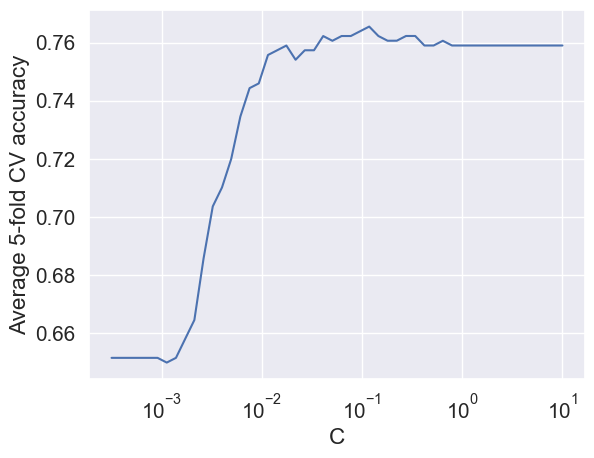
\includegraphics[keepaspectratio]{XGBoost_files/figure-pdf/cell-29-output-1.png}}

Tuning \texttt{scale\_pos\_weight} changes the \textbf{model's internal
learning dynamics}, not just the decision threshold. This allows the
model to adjust how it learns from imbalanced data.

In this case, as \texttt{scale\_pos\_weight} increases from 1 to 3:

\begin{itemize}
\tightlist
\item
  XGBoost starts giving \textbf{more importance to the minority
  (positive) class}.
\item
  The model becomes better at identifying \textbf{true positives} → ✅
  \textbf{Recall increases}
\item
  Simultaneously, it avoids more \textbf{false positives} → ✅
  \textbf{Precision increases}
\end{itemize}

✅ This indicates the model was previously \textbf{underperforming on
the positive class}, and that moderate rebalancing (e.g.,
\texttt{scale\_pos\_weight\ =\ 3}) helped improve \textbf{both recall
and precision} --- something that can happen when the model is initially
biased toward the majority class.

\subsection{Threshold adjustment}\label{threshold-adjustment}

\begin{Shaded}
\begin{Highlighting}[]
\CommentTok{\# get prediction probabilities}
\NormalTok{y\_diabetes\_pred\_proba }\OperatorTok{=}\NormalTok{ diabetes\_pipeline.predict\_proba(X\_diabetes\_test)[:, }\DecValTok{1}\NormalTok{]}

\CommentTok{\# plot the precision{-}recall curve}
\NormalTok{precision, recall, thresholds }\OperatorTok{=}\NormalTok{ precision\_recall\_curve(y\_diabetes\_test, y\_diabetes\_pred\_proba)}

\CommentTok{\# final threshold}
\NormalTok{f1\_scores }\OperatorTok{=} \DecValTok{2} \OperatorTok{*}\NormalTok{ (precision }\OperatorTok{*}\NormalTok{ recall) }\OperatorTok{/}\NormalTok{ (precision }\OperatorTok{+}\NormalTok{ recall }\OperatorTok{+} \FloatTok{1e{-}9}\NormalTok{) }\CommentTok{\# avoid division by zero}
\NormalTok{best\_f1\_threshold }\OperatorTok{=}\NormalTok{ thresholds[np.argmax(f1\_scores)]}
\NormalTok{best\_threshold }\OperatorTok{=}\NormalTok{ np.}\BuiltInTok{round}\NormalTok{(best\_f1\_threshold, }\DecValTok{2}\NormalTok{)}
\BuiltInTok{print}\NormalTok{(}\SpecialStringTok{f"Best Threshold for F1 Score: }\SpecialCharTok{\{}\NormalTok{best\_threshold}\SpecialCharTok{:.2f\}}\SpecialStringTok{"}\NormalTok{)}

\CommentTok{\# adjust the threshold for the predictions}
\NormalTok{y\_diabetes\_pred\_adjusted }\OperatorTok{=}\NormalTok{ (y\_diabetes\_pred\_proba }\OperatorTok{\textgreater{}=}\NormalTok{ best\_f1\_threshold).astype(}\BuiltInTok{int}\NormalTok{)}
\CommentTok{\# evaluate the model with the adjusted threshold}
\NormalTok{accuracy\_adjusted }\OperatorTok{=}\NormalTok{ np.mean(y\_diabetes\_pred\_adjusted }\OperatorTok{==}\NormalTok{ y\_diabetes\_test)}
\BuiltInTok{print}\NormalTok{(}\SpecialStringTok{f"Accuracy with Adjusted Threshold: }\SpecialCharTok{\{}\NormalTok{accuracy\_adjusted}\SpecialCharTok{:.2f\}}\SpecialStringTok{"}\NormalTok{)}
\NormalTok{precision\_adjusted }\OperatorTok{=}\NormalTok{ precision\_score(y\_diabetes\_test, y\_diabetes\_pred\_adjusted)}
\BuiltInTok{print}\NormalTok{(}\SpecialStringTok{f"Precision with Adjusted Threshold: }\SpecialCharTok{\{}\NormalTok{precision\_adjusted}\SpecialCharTok{:.2f\}}\SpecialStringTok{"}\NormalTok{)}
\NormalTok{recall\_adjusted }\OperatorTok{=}\NormalTok{ recall\_score(y\_diabetes\_test, y\_diabetes\_pred\_adjusted)}
\BuiltInTok{print}\NormalTok{(}\SpecialStringTok{f"Recall with Adjusted Threshold: }\SpecialCharTok{\{}\NormalTok{recall\_adjusted}\SpecialCharTok{:.2f\}}\SpecialStringTok{"}\NormalTok{)}
\CommentTok{\# plot the precision{-}recall curve}
\NormalTok{plt.figure(figsize}\OperatorTok{=}\NormalTok{(}\DecValTok{10}\NormalTok{, }\DecValTok{6}\NormalTok{))}
\NormalTok{plt.plot(recall, precision, marker}\OperatorTok{=}\StringTok{\textquotesingle{}o\textquotesingle{}}\NormalTok{)}
\NormalTok{plt.xlabel(}\StringTok{\textquotesingle{}Recall\textquotesingle{}}\NormalTok{, fontsize}\OperatorTok{=}\DecValTok{12}\NormalTok{)}
\NormalTok{plt.ylabel(}\StringTok{\textquotesingle{}Precision\textquotesingle{}}\NormalTok{, fontsize}\OperatorTok{=}\DecValTok{12}\NormalTok{)}
\NormalTok{plt.title(}\StringTok{\textquotesingle{}Precision{-}Recall Curve\textquotesingle{}}\NormalTok{, fontsize}\OperatorTok{=}\DecValTok{14}\NormalTok{)}
\NormalTok{plt.grid(}\VariableTok{True}\NormalTok{)}
\NormalTok{plt.axvline(x}\OperatorTok{=}\NormalTok{recall[np.argmax(f1\_scores)], color}\OperatorTok{=}\StringTok{\textquotesingle{}red\textquotesingle{}}\NormalTok{, linestyle}\OperatorTok{=}\StringTok{\textquotesingle{}{-}{-}\textquotesingle{}}\NormalTok{, label}\OperatorTok{=}\StringTok{\textquotesingle{}Best Threshold\textquotesingle{}}\NormalTok{)}
\NormalTok{plt.legend()}
\NormalTok{plt.tight\_layout()}
\NormalTok{plt.show()}
\end{Highlighting}
\end{Shaded}

\begin{verbatim}
Best Threshold for F1 Score: 0.19
Accuracy with Adjusted Threshold: 0.78
Precision with Adjusted Threshold: 0.68
Recall with Adjusted Threshold: 0.82
\end{verbatim}

\pandocbounded{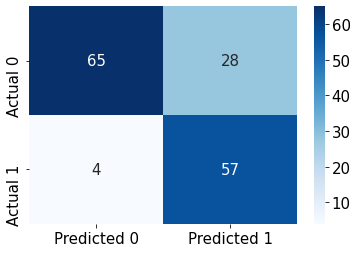
\includegraphics[keepaspectratio]{XGBoost_files/figure-pdf/cell-30-output-2.png}}

\subsection{\texorpdfstring{Alternative Method: Custom Instance Weights
(\texttt{sample\_weight})}{Alternative Method: Custom Instance Weights (sample\_weight)}}\label{alternative-method-custom-instance-weights-sample_weight}

You can assign \textbf{custom weights to individual training samples}
using the \texttt{sample\_weight} parameter in \texttt{fit()}
(scikit-learn API) or \texttt{weight} in \texttt{DMatrix} (native API).
This gives you \textbf{fine-grained control} over how much each sample
contributes to the loss and gradient during training.

Example (scikit-learn API):

\begin{Shaded}
\begin{Highlighting}[]
\ImportTok{from}\NormalTok{ xgboost }\ImportTok{import}\NormalTok{ XGBClassifier}
\ImportTok{import}\NormalTok{ numpy }\ImportTok{as}\NormalTok{ np}

\CommentTok{\# Assign higher weights to positive class}
\NormalTok{weights }\OperatorTok{=}\NormalTok{ np.where(y\_train }\OperatorTok{==} \DecValTok{1}\NormalTok{, }\DecValTok{5}\NormalTok{, }\DecValTok{1}\NormalTok{)}

\NormalTok{model }\OperatorTok{=}\NormalTok{ XGBClassifier()}
\NormalTok{model.fit(X\_train, y\_train, sample\_weight}\OperatorTok{=}\NormalTok{weights)}
\end{Highlighting}
\end{Shaded}

\textbf{When to Use This:}

\begin{itemize}
\item
  When you want more flexibility than scale\_pos\_weight allows
\item
  When the imbalance is complex (e.g., multi-class or cost-sensitive)
\item
  When you want to incorporate domain knowledge into weight assignments
\end{itemize}

\subsection{\texorpdfstring{\texttt{scale\_pos\_weight}
vs.~\texttt{sample\_weight}}{scale\_pos\_weight vs.~sample\_weight}}\label{scale_pos_weight-vs.-sample_weight}

\begin{longtable}[]{@{}
  >{\raggedright\arraybackslash}p{(\linewidth - 4\tabcolsep) * \real{0.1198}}
  >{\raggedright\arraybackslash}p{(\linewidth - 4\tabcolsep) * \real{0.4491}}
  >{\raggedright\arraybackslash}p{(\linewidth - 4\tabcolsep) * \real{0.4311}}@{}}
\toprule\noalign{}
\begin{minipage}[b]{\linewidth}\raggedright
\textbf{Feature}
\end{minipage} & \begin{minipage}[b]{\linewidth}\raggedright
\textbf{\texttt{scale\_pos\_weight}}
\end{minipage} & \begin{minipage}[b]{\linewidth}\raggedright
\textbf{\texttt{sample\_weight}}
\end{minipage} \\
\midrule\noalign{}
\endhead
\bottomrule\noalign{}
\endlastfoot
\textbf{Applies to} & Entire positive class (\texttt{label\ =\ 1}) &
Individual samples \\
\textbf{How it works} & Multiplies gradients and Hessians of the
positive class during training & Directly scales the loss function per
instance \\
\textbf{Use case} & Binary classification with class imbalance & Any
situation needing custom weighting (e.g., multi-class, domain-driven) \\
\textbf{Flexibility} & One global weight value & Full per-sample
control \\
\textbf{Where to set} & \texttt{scale\_pos\_weight} parameter in
\texttt{XGBClassifier} or \texttt{DMatrix} & \texttt{sample\_weight} in
\texttt{.fit()} or \texttt{weight=} in \texttt{DMatrix} \\
\end{longtable}

\section{Resources for Learning
XGBoost}\label{resources-for-learning-xgboost}

The foundational paper is:

\textbf{XGBoost: A Scalable Tree Boosting System}\\
\emph{Authors}: Tianqi Chen and Carlos Guestrin\\
\emph{Conference}: KDD 2016\\
\href{https://arxiv.org/abs/1603.02754}{Link to paper (PDF)}\\
\href{https://doi.org/10.1145/2939672.2939785}{DOI:
10.1145/2939672.2939785}

XGBoost is a relatively recent algorithm (2016), and thus not yet
included in many standard textbooks. Below are helpful learning
resources:

\begin{itemize}
\tightlist
\item
  \href{https://xgboost.readthedocs.io/en/stable/python/python_api.html}{Documentation}
\item
  \href{https://files.speakerdeck.com/presentations/5c6dab45648344208185d2b1ab4fdc95/XGBoost-Newest.pdf}{Slides
  by Tianqi Chen}
\item
  \href{https://dl.acm.org/doi/pdf/10.1145/2939672.2939785}{Reference
  Paper}
\item
  \href{https://www.youtube.com/watch?v=Vly8xGnNiWs}{Video by Tianqi
  Chen (author)}
\item
  \href{https://www.youtube.com/watch?v=OtD8wVaFm6E}{StatQuest Video
  Explanation}
\end{itemize}

\chapter{LightGBM and CatBoost}\label{lightgbm-and-catboost}

Gradient boosting is one of the most powerful techniques for
\textbf{structured/tabular data}, often serving as the \textbf{go-to
choice for tabular data tasks in machine learning competitions}.

In the previous chapter, we explored \textbf{XGBoost} in
detail---covering its \textbf{optimization objective},
\textbf{regularization techniques}, \textbf{split finding algorithms},
and its role as a cornerstone in modern \textbf{tabular modeling}.

While \textbf{XGBoost} is highly effective, other libraries have
introduced innovations to address challenges like scalability and
categorical feature handling. In this chapter, we focus on two
\textbf{advanced gradient boosting libraries} and their \textbf{key
innovations}:

\begin{itemize}
\item
  \textbf{LightGBM}: Developed by Microsoft, \textbf{LightGBM} is
  optimized for \textbf{speed and scalability}. It introduces
  \textbf{Gradient-based One-Side Sampling (GOSS)}, which prioritizes
  instances with larger gradients for faster training, and
  \textbf{Exclusive Feature Bundling (EFB)}, which reduces memory usage
  by grouping mutually exclusive features. \textbf{LightGBM} also
  supports \textbf{categorical features} efficiently, making it ideal
  for \textbf{large datasets and high-dimensional features}.
\item
  \textbf{CatBoost}: Created by Yandex, \textbf{CatBoost} excels in its
  \textbf{optimized support for categorical features} through advanced
  target-based encoding. It uses \textbf{ordered boosting} to prevent
  prediction shift and reduce overfitting, often performing well with
  \textbf{minimal tuning} on datasets rich in \textbf{categorical
  variables}.
\end{itemize}

\section{What They Share with
XGBoost}\label{what-they-share-with-xgboost}

While \textbf{LightGBM} and \textbf{CatBoost} introduce unique
innovations, they build on the same foundational principles as
\textbf{XGBoost}:

\begin{itemize}
\tightlist
\item
  They use a \textbf{similar objective function structure} (loss plus
  regularization) to balance model fit and complexity.
\item
  They apply a \textbf{second-order Taylor approximation} for efficient
  optimization of the loss function.
\item
  They support \textbf{histogram-based split-finding algorithms} to
  speed up training, with \textbf{LightGBM} particularly optimized for
  this approach.
\item
  They support \textbf{parallel tree building}, significantly
  accelerating training compared to traditional gradient boosting.
\item
  They provide \textbf{native support for categorical encoding},
  reducing the need for preprocessing (e.g., one-hot encoding), with
  \textbf{XGBoost} introducing this feature starting in version 1.5.0.
\end{itemize}

\section{LightGBM}\label{lightgbm}

\subsection{What is LightGBM?}\label{what-is-lightgbm}

\textbf{LightGBM} (Light Gradient Boosting Machine) is a
high-performance gradient boosting framework developed by Microsoft in
2017. Designed for \textbf{speed and scalability}, it is typically
faster than \textbf{XGBoost} due to its optimized algorithms, with
accuracy that is generally comparable but may require tuning. LightGBM
excels in:

\begin{itemize}
\tightlist
\item
  \textbf{Handling large-scale datasets} with many rows and features
\item
  \textbf{Achieving high speed and memory efficiency} through
  innovations like \textbf{Gradient-based One-Side Sampling (GOSS)},
  \textbf{Exclusive Feature Bundling (EFB)}, and \textbf{histogram-based
  splitting}
\end{itemize}

Like \textbf{XGBoost} and \textbf{CatBoost}, it supports \textbf{native
categorical encoding} and \textbf{parallel tree building}, enhancing its
efficiency for tabular data tasks. See the
\href{https://proceedings.neurips.cc/paper/2017/file/6449f44a102fde848669bdd9eb6b76fa-Paper.pdf}{LightGBM
paper} for details on its algorithmic innovations and performance
benchmarks.

\subsection{What Makes LightGBM Lighting
Fast?}\label{what-makes-lightgbm-lighting-fast}

LightGBM often outperforms XGBoost in \textbf{training speed} and
\textbf{memory efficiency}, thanks to several key innovations:

\subsubsection{Leaf-Wise Tree Growth}\label{leaf-wise-tree-growth}

\begin{itemize}
\tightlist
\item
  LightGBM splits the \textbf{leaf with the largest potential loss
  reduction}, unlike XGBoost's \textbf{level-wise} approach.
\item
  This leads to \textbf{lower loss per tree}, making learning more
  efficient --- though it may \textbf{overfit} without proper
  regularization.
\item
  Main controls:

  \begin{itemize}
  \tightlist
  \item
    \texttt{num\_leaves}: primary control for tree complexity
  \item
    \texttt{max\_depth}: optional constraint to prevent overfitting
  \end{itemize}
\end{itemize}

\subsubsection{GOSS (Gradient-based One-Side
Sampling)}\label{goss-gradient-based-one-side-sampling}

\begin{itemize}
\tightlist
\item
  GOSS improves speed by:

  \begin{itemize}
  \tightlist
  \item
    \textbf{Retaining all instances with large gradients} (i.e., high
    error)
  \item
    \textbf{Randomly sampling those with small gradients}
  \end{itemize}
\item
  This reduces the dataset size while maintaining accurate split
  decisions.
\end{itemize}

In gradient boosting, the tree is fit to the \textbf{negative gradient}
of the loss:

\[
r_m = -\left[ \frac{\partial L(y_i, f(x_i))}{\partial f(x_i)} \right]_{f = f_{m-1}}
\]

Observations with larger gradients have more influence on reducing the
loss --- GOSS prioritizes those. This approach reduces the number of
data points processed per iteration, speeding up training while
preserving important information.

\subsubsection{Exclusive Feature Bundling
(EFB)}\label{exclusive-feature-bundling-efb}

\begin{itemize}
\tightlist
\item
  \textbf{EFB} reduces memory usage and accelerates training by bundling
  \textbf{mutually exclusive} features (i.e., features that rarely have
  non-zero values simultaneously) in \textbf{high-dimensional sparse
  feature spaces}.
\item
  This is particularly effective for datasets with \textbf{many
  categorical variables} or \textbf{one-hot encoded features}, avoiding
  the memory overhead of one-hot encoding and complementing LightGBM's
  \textbf{native categorical support}.
\end{itemize}

\textbf{Example}:\\
The table below shows two mutually exclusive features, \texttt{feature1}
and \texttt{feature2}, bundled into a single \texttt{feature\_bundle} by
assigning distinct value ranges (e.g., 1--4 for \texttt{feature1}, 5--6
for \texttt{feature2}):

\begin{longtable}[]{@{}lll@{}}
\toprule\noalign{}
\texttt{feature1} & \texttt{feature2} & \texttt{feature\_bundle} \\
\midrule\noalign{}
\endhead
\bottomrule\noalign{}
\endlastfoot
0 & 2 & 6 \\
0 & 1 & 5 \\
0 & 2 & 6 \\
1 & 0 & 1 \\
2 & 0 & 2 \\
3 & 0 & 3 \\
4 & 0 & 4 \\
\end{longtable}

\begin{itemize}
\tightlist
\item
  \textbf{Hyperparameter for EFB}:

  \begin{itemize}
  \tightlist
  \item
    \texttt{enable\_bundle}: Enabled by default to activate automatic
    bundling.
  \item
    \texttt{max\_conflict\_rate}: Controls the maximum conflict rate for
    bundling (default: 0.0, no conflicts allowed); adjust (e.g., 0.1) to
    allow minor overlaps.
  \end{itemize}
\end{itemize}

This approach reduces the number of features processed per iteration,
speeding up training while preserving important information.

Combined with \textbf{GOSS}, \textbf{EFB} makes \textbf{LightGBM}
especially well-suited for \textbf{large-scale, sparse, tabular
datasets}, offering \textbf{speed and scalability} while maintaining
comparable accuracy with proper tuning.

\subsection{Using LightGBM}\label{using-lightgbm}

Although \textbf{LightGBM is not part of Scikit-learn}, it provides a
\textbf{Scikit-learn-compatible API} through the
\texttt{lightgbm.sklearn} module. This allows you to use LightGBM models
seamlessly with Scikit-learn tools such as \texttt{Pipeline},
\texttt{GridSearchCV}, and \texttt{cross\_val\_score}.

The main classes are:

\begin{itemize}
\tightlist
\item
  \href{https://lightgbm.readthedocs.io/en/latest/pythonapi/lightgbm.LGBMRegressor.html}{\texttt{LGBMRegressor}}:
  for regression tasks\\
\item
  \href{https://lightgbm.readthedocs.io/en/latest/pythonapi/lightgbm.LGBMClassifier.html}{\texttt{LGBMClassifier}}:
  for classification tasks
\end{itemize}

To install the package:

\begin{Shaded}
\begin{Highlighting}[]
\NormalTok{pip install lightgbm}
\end{Highlighting}
\end{Shaded}

\begin{quote}
\textbf{Note:} LightGBM is a separate library, not part of Scikit-learn,
but it provides a \textbf{Scikit-learn-compatible API} via
\texttt{LGBMClassifier} and \texttt{LGBMRegressor}.\\
This makes it easy to integrate LightGBM models into Scikit-learn
workflows such as \texttt{Pipeline}, \texttt{GridSearchCV}, and
\texttt{cross\_val\_score}.
\end{quote}

\subsubsection{Core LightGBM
Hyperparameters}\label{core-lightgbm-hyperparameters}

\textbf{Core Tree Structure}:

\begin{itemize}
\tightlist
\item
  \texttt{num\_leaves}: Maximum number of leaves (terminal nodes) per
  tree.
\item
  \texttt{min\_data\_in\_leaf}: Minimum number of data points required
  in a leaf.
\item
  \texttt{max\_depth}: Maximum depth of a tree (used to control
  overfitting).
\end{itemize}

\textbf{Learning Control and Regularization}:

\begin{itemize}
\tightlist
\item
  \texttt{learning\_rate\ (η)}: Shrinks the contribution of each tree.
\item
  \texttt{n\_estimators}: Number of boosting rounds.
\item
  \texttt{lambda\_l1} / \texttt{lambda\_l2}: L1 and L2 regularization on
  leaf weights.
\item
  \texttt{min\_gain\_to\_split}: Minimum loss reduction required to make
  a further split (structure regularization).
\end{itemize}

\textbf{Data Handling}:

\begin{itemize}
\tightlist
\item
  \texttt{feature\_fraction}: Fraction of features randomly sampled for
  each tree (a.k.a. \texttt{colsample\_bytree} in XGBoost).
\item
  \texttt{bagging\_fraction}: Fraction of data randomly sampled for each
  iteration.
\item
  \texttt{bagging\_freq}: Frequency (in iterations) to perform bagging.
\item
  \texttt{categorical\_feature}: Specifies which features are
  categorical (enables native handling).
\end{itemize}

\textbf{Speed vs.~Accuracy Trade-offs}:

\begin{itemize}
\tightlist
\item
  \texttt{max\_bin}: Number of bins used to bucket continuous features.
\item
  \texttt{data\_sample\_strategy} : \texttt{bagging} or \texttt{goss}
\item
  \texttt{top\_rate} \emph{(\texttt{goss} only)}: Fraction of instances
  with the largest gradients to keep.
\item
  \texttt{other\_rate} \emph{(\texttt{goss} only)}: Fraction of
  small-gradient instances to randomly sample. -\texttt{enable\_bundle}:
  set this to true to spped up the training for sparse datasets
\end{itemize}

\textbf{Optimization Control}:

\begin{itemize}
\tightlist
\item
  \texttt{boosting}: Type of boosting algorithm (\texttt{gbdt},
  \texttt{dart}, \texttt{rf}, etc.).
\item
  \texttt{early\_stopping\_rounds}: Stops training if the validation
  score doesn't improve over a set number of rounds.
\end{itemize}

\textbf{Imbalanced Data}

\begin{itemize}
\tightlist
\item
  \texttt{scale\_pos\_weight}: Manually sets the weight for the positive
  class in binary classification.
\item
  \texttt{is\_unbalance}: Automatically adjusts class weights based on
  the training data distribution.
\end{itemize}

\begin{quote}
⚠️ These two options are \textbf{mutually exclusive} --- use
\textbf{only one}. If both are set, \texttt{scale\_pos\_weight} takes
priority.
\end{quote}

For full details and advanced options, see the
\href{https://lightgbm.readthedocs.io/en/latest/Parameters.html}{LightGBM
Parameters Guide}.

\begin{Shaded}
\begin{Highlighting}[]
\ImportTok{import}\NormalTok{ pandas }\ImportTok{as}\NormalTok{ pd}
\ImportTok{import}\NormalTok{ numpy }\ImportTok{as}\NormalTok{ np}
\ImportTok{import}\NormalTok{ matplotlib.pyplot }\ImportTok{as}\NormalTok{ plt}
\ImportTok{from}\NormalTok{ sklearn.model\_selection }\ImportTok{import}\NormalTok{ train\_test\_split, GridSearchCV}
\ImportTok{from}\NormalTok{ sklearn.preprocessing }\ImportTok{import}\NormalTok{ OneHotEncoder, StandardScaler}
\ImportTok{from}\NormalTok{ sklearn.compose }\ImportTok{import}\NormalTok{ ColumnTransformer}
\ImportTok{from}\NormalTok{ sklearn.pipeline }\ImportTok{import}\NormalTok{ Pipeline}
\ImportTok{from}\NormalTok{ sklearn.metrics }\ImportTok{import}\NormalTok{ root\_mean\_squared\_error, r2\_score, accuracy\_score, precision\_score, recall\_score, f1\_score, precision\_recall\_curve}
\ImportTok{from}\NormalTok{ xgboost }\ImportTok{import}\NormalTok{ XGBRegressor, XGBClassifier}
\ImportTok{import}\NormalTok{ lightgbm }\ImportTok{as}\NormalTok{ lgb}
\ImportTok{import}\NormalTok{ seaborn }\ImportTok{as}\NormalTok{ sns}

\ImportTok{from}\NormalTok{ skopt }\ImportTok{import}\NormalTok{ BayesSearchCV}
\ImportTok{from}\NormalTok{ skopt.space }\ImportTok{import}\NormalTok{ Real, Categorical, Integer}
\ImportTok{from}\NormalTok{ skopt.plots }\ImportTok{import}\NormalTok{ plot\_objective, plot\_histogram, plot\_convergence}
\ImportTok{import}\NormalTok{ warnings}
\end{Highlighting}
\end{Shaded}

We'll continue to use the same datasets that we have been using
throughout the course.

\begin{Shaded}
\begin{Highlighting}[]
\CommentTok{\# Load the dataset}
\NormalTok{car }\OperatorTok{=}\NormalTok{ pd.read\_csv(}\StringTok{\textquotesingle{}Datasets/car.csv\textquotesingle{}}\NormalTok{)}
\NormalTok{car.head()}
\end{Highlighting}
\end{Shaded}

\begin{longtable}[]{@{}lllllllllll@{}}
\toprule\noalign{}
& brand & model & year & transmission & mileage & fuelType & tax & mpg &
engineSize & price \\
\midrule\noalign{}
\endhead
\bottomrule\noalign{}
\endlastfoot
0 & vw & Beetle & 2014 & Manual & 55457 & Diesel & 30 & 65.3266 & 1.6 &
7490 \\
1 & vauxhall & GTC & 2017 & Manual & 15630 & Petrol & 145 & 47.2049 &
1.4 & 10998 \\
2 & merc & G Class & 2012 & Automatic & 43000 & Diesel & 570 & 25.1172 &
3.0 & 44990 \\
3 & audi & RS5 & 2019 & Automatic & 10 & Petrol & 145 & 30.5593 & 2.9 &
51990 \\
4 & merc & X-CLASS & 2018 & Automatic & 14000 & Diesel & 240 & 35.7168 &
2.3 & 28990 \\
\end{longtable}

\begin{Shaded}
\begin{Highlighting}[]
\NormalTok{X }\OperatorTok{=}\NormalTok{ car.drop(columns}\OperatorTok{=}\NormalTok{[}\StringTok{\textquotesingle{}price\textquotesingle{}}\NormalTok{])}
\NormalTok{y }\OperatorTok{=}\NormalTok{ car[}\StringTok{\textquotesingle{}price\textquotesingle{}}\NormalTok{]}

\CommentTok{\# extract the categorical columns and put them in a list}
\NormalTok{categorical\_feature }\OperatorTok{=}\NormalTok{ X.select\_dtypes(include}\OperatorTok{=}\NormalTok{[}\StringTok{\textquotesingle{}object\textquotesingle{}}\NormalTok{]).columns.tolist()}

\CommentTok{\# extract the numerical columns and put them in a list}
\NormalTok{numerical\_feature }\OperatorTok{=}\NormalTok{ X.select\_dtypes(include}\OperatorTok{=}\NormalTok{[}\StringTok{\textquotesingle{}int64\textquotesingle{}}\NormalTok{, }\StringTok{\textquotesingle{}float64\textquotesingle{}}\NormalTok{]).columns.tolist()}

\CommentTok{\# convert the categorical columns to category type}
\ControlFlowTok{for}\NormalTok{ col }\KeywordTok{in}\NormalTok{ categorical\_feature:}
\NormalTok{    X[col] }\OperatorTok{=}\NormalTok{ X[col].astype(}\StringTok{\textquotesingle{}category\textquotesingle{}}\NormalTok{)}


\CommentTok{\# Split the data into training and testing sets}
\NormalTok{X\_train, X\_test, y\_train, y\_test }\OperatorTok{=}\NormalTok{ train\_test\_split(X, y, test\_size}\OperatorTok{=}\FloatTok{0.2}\NormalTok{, random\_state}\OperatorTok{=}\DecValTok{42}\NormalTok{)}
\end{Highlighting}
\end{Shaded}

\subsubsection{Building a Baseline Model Using LightGBM's Native
Categorical Feature
Support}\label{building-a-baseline-model-using-lightgbms-native-categorical-feature-support}

LightGBM provides \textbf{built-in support for handling categorical
features}, eliminating the need for manual encoding (like one-hot or
ordinal encoding). By directly passing categorical column names or
indices to the model, LightGBM can internally apply efficient encoding
and optimized split finding for categorical variables.

In this section, we'll use this native capability to \textbf{quickly
build a baseline model}, taking advantage of LightGBM's efficiency with
structured data that includes categorical columns.

This baseline model serves as a \textbf{starting point} for comparison
against more advanced tuning

\begin{Shaded}
\begin{Highlighting}[]
\OperatorTok{\%\%}\NormalTok{time}
\CommentTok{\# ===== 1. Baseline Model =====}
\BuiltInTok{print}\NormalTok{(}\StringTok{"}\CharTok{\textbackslash{}n}\StringTok{===== Baseline LightGBM Model ====="}\NormalTok{)}
\CommentTok{\# Initialize the LightGBM regressor}
\NormalTok{model }\OperatorTok{=}\NormalTok{ lgb.LGBMRegressor(random\_state}\OperatorTok{=}\DecValTok{42}\NormalTok{)}

\CommentTok{\# Train the model with categorical features specified}
\NormalTok{model.fit(}
\NormalTok{    X\_train, }
\NormalTok{    y\_train,}
\NormalTok{    categorical\_feature}\OperatorTok{=}\NormalTok{categorical\_feature}
\NormalTok{)}

\CommentTok{\# Predict on the test set}
\NormalTok{y\_pred }\OperatorTok{=}\NormalTok{ model.predict(X\_test)}

\CommentTok{\# Calculate evaluation metrics}
\NormalTok{rmse }\OperatorTok{=}\NormalTok{ root\_mean\_squared\_error(y\_test, y\_pred)}
\NormalTok{r2 }\OperatorTok{=}\NormalTok{ r2\_score(y\_test, y\_pred)}

\CommentTok{\# Output results}
\BuiltInTok{print}\NormalTok{(}\SpecialStringTok{f"Test RMSE: }\SpecialCharTok{\{}\NormalTok{rmse}\SpecialCharTok{:.4f\}}\SpecialStringTok{"}\NormalTok{)}
\BuiltInTok{print}\NormalTok{(}\SpecialStringTok{f"Test R²: }\SpecialCharTok{\{}\NormalTok{r2}\SpecialCharTok{:.4f\}}\SpecialStringTok{"}\NormalTok{)}
\end{Highlighting}
\end{Shaded}

\begin{verbatim}

===== Baseline LightGBM Model =====
Test RMSE: 3680.8999
Test R²: 0.9538
CPU times: total: 875 ms
Wall time: 82.6 ms
\end{verbatim}

\subsubsection{Enabling GOSS and EFB in
LightGBM}\label{enabling-goss-and-efb-in-lightgbm}

\paragraph{\texorpdfstring{GOSS is \textbf{not enabled by
default}.}{GOSS is not enabled by default.}}\label{goss-is-not-enabled-by-default.}

The default boosting type is \texttt{gbdt} (traditional Gradient
Boosting Decision Tree), which uses all data instances for each
iteration without sampling based on gradients.

To use GOSS, you must explicitly set the \texttt{boosting\_type}
parameter to \texttt{goss} in the model configuration. When you do this,
LightGBM uses GOSS with default values for its specific hyperparameters:

\begin{itemize}
\tightlist
\item
  \texttt{top\_rate}: 0.2 (keeps 20\% of instances with large gradients)
\item
  \texttt{other\_rate}: 0.1 (randomly samples 10\% of instances with
  small gradients)
\end{itemize}

\paragraph{\texorpdfstring{EFB is \textbf{enabled by
default}}{EFB is enabled by default}}\label{efb-is-enabled-by-default}

\begin{Shaded}
\begin{Highlighting}[]
\NormalTok{enable\_bundle }\OperatorTok{=} \VariableTok{True}
\end{Highlighting}
\end{Shaded}

This optimization reduces dimensionality by bundling mutually exclusive
sparse features, such as those resulting from one-hot encoding.

⚠️ Note: In our car dataset, the data size is small and there are only a
few categorical features, so these optimizations may not have a
noticeable impact. However, for large-scale datasets with many
categorical features, enabling GOSS and EFB is highly recommended to
improve training efficiency and reduce memory usage.

\begin{Shaded}
\begin{Highlighting}[]
\OperatorTok{\%\%}\NormalTok{time}
\CommentTok{\# ===== 2. LightGBM with GOSS Sampling =====}
\BuiltInTok{print}\NormalTok{(}\StringTok{"}\CharTok{\textbackslash{}n}\StringTok{===== LightGBM with GOSS Sampling ====="}\NormalTok{)}

\CommentTok{\# Initialize the LightGBM regressor with GOSS}
\NormalTok{model\_goss }\OperatorTok{=}\NormalTok{ lgb.LGBMRegressor(}
\NormalTok{    boosting\_type}\OperatorTok{=}\StringTok{\textquotesingle{}goss\textquotesingle{}}\NormalTok{,}
\NormalTok{    random\_state}\OperatorTok{=}\DecValTok{42}
\NormalTok{)}

\CommentTok{\# Train the model with categorical features specified}
\NormalTok{model\_goss.fit(}
\NormalTok{    X\_train,}
\NormalTok{    y\_train,}
\NormalTok{    categorical\_feature}\OperatorTok{=}\NormalTok{categorical\_feature}
\NormalTok{)}

\CommentTok{\# Predict on the test set}
\NormalTok{y\_pred\_goss }\OperatorTok{=}\NormalTok{ model\_goss.predict(X\_test)}

\CommentTok{\# Calculate evaluation metrics}
\NormalTok{rmse\_goss }\OperatorTok{=}\NormalTok{ root\_mean\_squared\_error(y\_test, y\_pred\_goss)}
\NormalTok{r2\_goss }\OperatorTok{=}\NormalTok{ r2\_score(y\_test, y\_pred\_goss)}

\CommentTok{\# Output results}
\BuiltInTok{print}\NormalTok{(}\SpecialStringTok{f"Test RMSE (GOSS): }\SpecialCharTok{\{}\NormalTok{rmse\_goss}\SpecialCharTok{:.4f\}}\SpecialStringTok{"}\NormalTok{)}
\BuiltInTok{print}\NormalTok{(}\SpecialStringTok{f"Test R² (GOSS): }\SpecialCharTok{\{}\NormalTok{r2\_goss}\SpecialCharTok{:.4f\}}\SpecialStringTok{"}\NormalTok{)}
\end{Highlighting}
\end{Shaded}

\begin{verbatim}

===== LightGBM with GOSS Sampling =====
Test RMSE (GOSS): 3510.7726
Test R² (GOSS): 0.9580
CPU times: total: 766 ms
Wall time: 79.6 ms
\end{verbatim}

\subsubsection{\texorpdfstring{Tuning \texttt{top\_rate} and
\texttt{other\_rate} in
GOSS}{Tuning top\_rate and other\_rate in GOSS}}\label{tuning-top_rate-and-other_rate-in-goss}

Even with this small dataset, we observed a \textbf{shorter execution
time} and a \textbf{slight improvement in performance} using GOSS.

The default settings are reasonable for many datasets. To leverage
\textbf{GOSS} more effectively, optimize performance by tuning
\textbf{top\_rate} (e.g., 0.1, 0.2, 0.3, 0.4) and \textbf{other\_rate}
(e.g., 0.05, 0.1, 0.15, 0.2) using cross-validation, especially for
large or noisy datasets.

\begin{quote}
⚠️ \textbf{Note:} When using
\texttt{boosting\_type=\textquotesingle{}goss\textquotesingle{}},
LightGBM requires that\\
\textbf{\texttt{top\_rate\ +\ other\_rate\ ≤\ 1.0}}\strut \\
This constraint ensures that the combined sample used for training does
not exceed the size of the full dataset.
\end{quote}

\begin{Shaded}
\begin{Highlighting}[]
\CommentTok{\# tuning the top\_rate and other\_rate parameters}
\CommentTok{\# Initialize the LightGBM regressor with GOSS}
\NormalTok{model\_goss\_tune }\OperatorTok{=}\NormalTok{ lgb.LGBMRegressor(}
\NormalTok{    boosting\_type}\OperatorTok{=}\StringTok{\textquotesingle{}goss\textquotesingle{}}\NormalTok{,}
\NormalTok{    random\_state}\OperatorTok{=}\DecValTok{42}
\NormalTok{)}
\CommentTok{\# Define the parameter grid for tuning}
\NormalTok{param\_grid }\OperatorTok{=}\NormalTok{ \{}
    \StringTok{\textquotesingle{}top\_rate\textquotesingle{}}\NormalTok{: Real(}\FloatTok{0.1}\NormalTok{, }\FloatTok{0.6}\NormalTok{, prior}\OperatorTok{=}\StringTok{\textquotesingle{}uniform\textquotesingle{}}\NormalTok{),}
    \StringTok{\textquotesingle{}other\_rate\textquotesingle{}}\NormalTok{: Real(}\FloatTok{0.1}\NormalTok{, }\FloatTok{0.4}\NormalTok{, prior}\OperatorTok{=}\StringTok{\textquotesingle{}uniform\textquotesingle{}}\NormalTok{),}
\NormalTok{\}}
\CommentTok{\# Initialize the BayesSearchCV object}
\NormalTok{opt }\OperatorTok{=}\NormalTok{ BayesSearchCV(}
\NormalTok{    model\_goss\_tune,}
\NormalTok{    param\_grid,}
\NormalTok{    n\_iter}\OperatorTok{=}\DecValTok{10}\NormalTok{,}
\NormalTok{    cv}\OperatorTok{=}\DecValTok{3}\NormalTok{,}
\NormalTok{    n\_jobs}\OperatorTok{={-}}\DecValTok{1}\NormalTok{,}
\NormalTok{    random\_state}\OperatorTok{=}\DecValTok{42}
\NormalTok{)}
\CommentTok{\# Fit the model}
\NormalTok{opt.fit(}
\NormalTok{    X\_train,}
\NormalTok{    y\_train,}
\NormalTok{    categorical\_feature}\OperatorTok{=}\NormalTok{categorical\_feature}
\NormalTok{)}
\CommentTok{\# the best parameters}
\BuiltInTok{print}\NormalTok{(}\StringTok{"Best parameters found: "}\NormalTok{, opt.best\_params\_)}

\CommentTok{\# Predict on the test set}
\NormalTok{y\_pred\_opt }\OperatorTok{=}\NormalTok{ opt.predict(X\_test)}

\CommentTok{\# Calculate evaluation metrics}
\NormalTok{rmse\_opt }\OperatorTok{=}\NormalTok{ root\_mean\_squared\_error(y\_test, y\_pred\_opt)}
\NormalTok{r2\_opt }\OperatorTok{=}\NormalTok{ r2\_score(y\_test, y\_pred\_opt)}
\CommentTok{\# Output results}
\BuiltInTok{print}\NormalTok{(}\SpecialStringTok{f"Test RMSE (GOSS with tuning): }\SpecialCharTok{\{}\NormalTok{rmse\_opt}\SpecialCharTok{:.4f\}}\SpecialStringTok{"}\NormalTok{)}
\BuiltInTok{print}\NormalTok{(}\SpecialStringTok{f"Test R² (GOSS with tuning): }\SpecialCharTok{\{}\NormalTok{r2\_opt}\SpecialCharTok{:.4f\}}\SpecialStringTok{"}\NormalTok{)}
\end{Highlighting}
\end{Shaded}

\begin{verbatim}
Best parameters found:  OrderedDict({'other_rate': 0.33986603248215197, 'top_rate': 0.31901459322046166})
Test RMSE (GOSS with tuning): 3458.7664
Test R² (GOSS with tuning): 0.9592
\end{verbatim}

\subsubsection{\texorpdfstring{Optimizing LightGBM with
\texttt{BayesSearchCV}}{Optimizing LightGBM with BayesSearchCV}}\label{optimizing-lightgbm-with-bayessearchcv}

\texttt{BayesSearchCV} from \texttt{scikit-optimize} provides an
efficient way to tune hyperparameters. Here's how to set this up:

\begin{Shaded}
\begin{Highlighting}[]
\OperatorTok{\%\%}\NormalTok{time}
\CommentTok{\# ===== 2. Hyperparameter Tuning with Bayesian Optimization =====}
\CommentTok{\# Define the parameter space for Bayesian optimization}
\NormalTok{param\_space }\OperatorTok{=}\NormalTok{ \{}
    \StringTok{\textquotesingle{}num\_leaves\textquotesingle{}}\NormalTok{: Integer(}\DecValTok{20}\NormalTok{, }\DecValTok{100}\NormalTok{),}
    \StringTok{\textquotesingle{}max\_depth\textquotesingle{}}\NormalTok{: Integer(}\DecValTok{5}\NormalTok{, }\DecValTok{50}\NormalTok{),}
    \StringTok{\textquotesingle{}min\_data\_in\_leaf\textquotesingle{}}\NormalTok{: Integer(}\DecValTok{1}\NormalTok{, }\DecValTok{100}\NormalTok{),}
    \StringTok{\textquotesingle{}learning\_rate\textquotesingle{}}\NormalTok{: Real(}\FloatTok{0.01}\NormalTok{, }\FloatTok{0.5}\NormalTok{, prior}\OperatorTok{=}\StringTok{\textquotesingle{}uniform\textquotesingle{}}\NormalTok{),}
    \StringTok{\textquotesingle{}n\_estimators\textquotesingle{}}\NormalTok{: Integer(}\DecValTok{50}\NormalTok{, }\DecValTok{500}\NormalTok{),}
    \StringTok{\textquotesingle{}top\_rate\textquotesingle{}}\NormalTok{: Real(}\FloatTok{0.1}\NormalTok{, }\FloatTok{0.6}\NormalTok{, prior}\OperatorTok{=}\StringTok{\textquotesingle{}uniform\textquotesingle{}}\NormalTok{),}
    \StringTok{\textquotesingle{}other\_rate\textquotesingle{}}\NormalTok{: Real(}\FloatTok{0.1}\NormalTok{, }\FloatTok{0.4}\NormalTok{, prior}\OperatorTok{=}\StringTok{\textquotesingle{}uniform\textquotesingle{}}\NormalTok{),}
\NormalTok{\}}
\CommentTok{\# Create the Bayesian search object}
\NormalTok{bayes\_search }\OperatorTok{=}\NormalTok{ BayesSearchCV(}
    \CommentTok{\# using verbose={-}1 to suppress warnings}
    \CommentTok{\# using n\_jobs={-}1 to use all available cores}
    \CommentTok{\# using random\_state=42 for reproducibility}
\NormalTok{    estimator}\OperatorTok{=}\NormalTok{lgb.LGBMRegressor( categorical\_feature}\OperatorTok{=}\NormalTok{categorical\_feature, random\_state}\OperatorTok{=}\DecValTok{42}\NormalTok{, boosting\_type}\OperatorTok{=}\StringTok{\textquotesingle{}goss\textquotesingle{}}\NormalTok{, verbose}\OperatorTok{={-}}\DecValTok{1}\NormalTok{),}
    \CommentTok{\# Define the parameter space for Bayesian optimization}
\NormalTok{    search\_spaces}\OperatorTok{=}\NormalTok{param\_space,}
\NormalTok{    n\_iter}\OperatorTok{=}\DecValTok{50}\NormalTok{,}
\NormalTok{    scoring}\OperatorTok{=}\StringTok{\textquotesingle{}neg\_root\_mean\_squared\_error\textquotesingle{}}\NormalTok{,}
\NormalTok{    cv}\OperatorTok{=}\DecValTok{3}\NormalTok{,}
\NormalTok{    n\_jobs}\OperatorTok{={-}}\DecValTok{1}\NormalTok{,}
\NormalTok{    random\_state}\OperatorTok{=}\DecValTok{42}
\NormalTok{)}
\CommentTok{\# Fit the Bayesian search object to the training data}
\NormalTok{bayes\_search.fit(X\_train, y\_train)}
\CommentTok{\# Get the best parameters and score}
\NormalTok{best\_params }\OperatorTok{=}\NormalTok{ bayes\_search.best\_params\_}
\NormalTok{best\_score }\OperatorTok{=}\NormalTok{ bayes\_search.best\_score\_}
\BuiltInTok{print}\NormalTok{(}\SpecialStringTok{f"Best Parameters: }\SpecialCharTok{\{}\NormalTok{best\_params}\SpecialCharTok{\}}\SpecialStringTok{"}\NormalTok{)}
\BuiltInTok{print}\NormalTok{(}\SpecialStringTok{f"Best Score: }\SpecialCharTok{\{}\NormalTok{best\_score}\SpecialCharTok{\}}\SpecialStringTok{"}\NormalTok{)}
\CommentTok{\# Get the best model}
\NormalTok{best\_model }\OperatorTok{=}\NormalTok{ bayes\_search.best\_estimator\_}
\CommentTok{\# Make predictions on the test set}
\NormalTok{y\_pred\_bayes }\OperatorTok{=}\NormalTok{ best\_model.predict(X\_test)}
\CommentTok{\# Calculate RMSE and R2 score for the best model}
\NormalTok{rmse\_bayes }\OperatorTok{=}\NormalTok{ root\_mean\_squared\_error(y\_test, y\_pred\_bayes)}
\NormalTok{r2\_bayes }\OperatorTok{=}\NormalTok{ r2\_score(y\_test, y\_pred\_bayes)}
\BuiltInTok{print}\NormalTok{(}\SpecialStringTok{f"RMSE (Bayesian Optimized): }\SpecialCharTok{\{}\NormalTok{rmse\_bayes}\SpecialCharTok{\}}\SpecialStringTok{"}\NormalTok{)}
\BuiltInTok{print}\NormalTok{(}\SpecialStringTok{f"R2 Score (Bayesian Optimized): }\SpecialCharTok{\{}\NormalTok{r2\_bayes}\SpecialCharTok{\}}\SpecialStringTok{"}\NormalTok{)}
\end{Highlighting}
\end{Shaded}

\begin{verbatim}
Best Parameters: OrderedDict({'learning_rate': 0.31777940485083805, 'max_depth': 5, 'min_data_in_leaf': 47, 'n_estimators': 369, 'num_leaves': 20, 'other_rate': 0.4, 'top_rate': 0.6})
Best Score: -3361.8218393725633
RMSE (Bayesian Optimized): 3071.418344800289
R2 Score (Bayesian Optimized): 0.9678447743461689
CPU times: total: 49.4 s
Wall time: 1min 35s
\end{verbatim}

\textbf{LightGBM} achieved performance comparable to \textbf{XGBoost}.
By leveraging \textbf{GOSS} (Gradient-based One-Side Sampling) for
gradient sampling and \textbf{EFB} (Exclusive Feature Bundling) for
feature reduction, it improved training speed slightly on large, sparse
datasets. These optimizations, along with \textbf{native categorical
feature support}, can also help reduce cross-validation tuning time by
simplifying the feature space and accelerating learning.

\section{CatBoost}\label{catboost}

\subsection{What is CatBoost?}\label{what-is-catboost}

\textbf{CatBoost} (short for \emph{Categorical Boosting}) is a
high-performance gradient boosting framework developed by
\textbf{Yandex}. While several modern boosting frameworks support native
categorical features, CatBoost uses \textbf{optimized encoding
strategies}---such as \textbf{ordered target statistics}---that often
lead to better performance with less risk of overfitting on
\textbf{categorical-heavy} data.

In addition to its categorical handling, CatBoost includes features like
\textbf{ordered boosting} and strong \textbf{regularization}, which help
reduce overfitting. It typically requires \textbf{less hyperparameter
tuning} than XGBoost or LightGBM, making it more \textbf{user-friendly},
especially on datasets with many categorical variables.

\subsection{What Makes CatBoost
Unique?}\label{what-makes-catboost-unique}

CatBoost introduces several \textbf{key innovations} that set it apart
from other gradient boosting frameworks:

\subsubsection{Symmetric (Oblivious)
Trees}\label{symmetric-oblivious-trees}

CatBoost builds \textbf{symmetric (oblivious) decision trees}, where the
same feature and split threshold are used at each level of the tree
across all nodes. This structure results in:

\begin{itemize}
\tightlist
\item
  \textbf{Robust to noise}
\item
  \textbf{Improved regularization}
\item
  \textbf{Faster inference times}
\end{itemize}

\subsubsection{Advanced Categorical Feature
Handling}\label{advanced-categorical-feature-handling}

CatBoost can \textbf{natively process categorical features} using an
approach based on \textbf{ordered target statistics}, which:

\begin{itemize}
\tightlist
\item
  Avoids target leakage during training
\item
  Typically outperforms traditional encodings like one-hot or label
  encoding
\end{itemize}

\subsubsection{Ordered Boosting (vs.~Standard
Boosting)}\label{ordered-boosting-vs.-standard-boosting}

Traditional gradient boosting algorithms often suffer from
\textbf{prediction shift}, a form of overfitting that occurs when the
model uses the same data to compute residuals and to fit new trees.

CatBoost addresses this with \textbf{ordered boosting}, a
permutation-driven strategy that builds each tree on one subset of data
and computes residuals on another (unseen) subset.

Recall that gradient boosting fits trees on the gradient of the loss
function:

\[
r_m = -\left[ \frac{\partial L(y_i, f(x_i))}{\partial f(x_i)} \right]_{f = f_{m-1}}
\]

In classic boosting, this gradient is calculated using the same training
observations that were used to fit the model, which leads to target
leakage.

In contrast, CatBoost:

\begin{itemize}
\tightlist
\item
  Shuffles the data at each iteration
\item
  Computes residuals for an observation \textbf{only from prior
  observations} in the permutation
\item
  Ensures that \textbf{each gradient estimate is based on unseen data}
\end{itemize}

This significantly improves the model's \textbf{generalizability} and
reduces overfitting, especially on \textbf{small or noisy datasets}.

\subsubsection{Handling of Text and Embedding
Features}\label{handling-of-text-and-embedding-features}

CatBoost can process text features directly by converting them into
numerical representations (e.g., using bag-of-words or embeddings)
within the model, reducing the need for external preprocessing. It also
supports integration with pre-trained embeddings, which is useful for
natural language processing (NLP) tasks.

Together, these innovations make CatBoost a strong candidate for
modeling \textbf{high-dimensional, categorical, and imbalanced tabular
data}, even with minimal feature engineering or hyperparameter tuning.

\subsubsection{Ease of Use and Defaults}\label{ease-of-use-and-defaults}

CatBoost's default hyperparameters are well-tuned for a wide range of
problems, reducing the need for extensive tuning. For example, its
learning rate, depth, and regularization parameters often yield strong
performance out of the box. In the paper, the authors also showed that
CatBoost outperforms XGBoost and LightGBM without tuning, i.e., with
default hyperparameter settings.

Read the
\href{https://proceedings.neurips.cc/paper_files/paper/2018/file/14491b756b3a51daac41c24863285549-Paper.pdf}{CatBoost
paper} for more details.

Here is a good
\href{https://neptune.ai/blog/when-to-choose-catboost-over-xgboost-or-lightgbm}{blog}
listing the key features of CatBoost.

\subsection{Using CatBoost}\label{using-catboost}

CatBoost provides a \textbf{scikit-learn-compatible API} through
\texttt{CatBoostClassifier} and \texttt{CatBoostRegressor}, which makes
it easy to integrate into pipelines and use with tools like
\texttt{GridSearchCV}, \texttt{cross\_val\_score}, and
\texttt{train\_test\_split}.

\subsection{Installation}\label{installation}

To install CatBoost, run:

\begin{Shaded}
\begin{Highlighting}[]
\NormalTok{pip install catboost}
\end{Highlighting}
\end{Shaded}

\begin{quote}
💡 GPU users: CatBoost automatically detects and uses GPU if available.
You can explicitly enable it with
\texttt{task\_type=\textquotesingle{}GPU\textquotesingle{}}.
\end{quote}

\subsection{CatBoost for Regression}\label{catboost-for-regression}

Let us check the performance of \texttt{CatBoostRegressor()} without
tuning, i.e., with default hyperparameter settings on our car dataset

The parameter \texttt{cat\_features} will be used to specify the indices
of the categorical predictors for target encoding.

\begin{Shaded}
\begin{Highlighting}[]
\CommentTok{\# build a catboostregressor model}
\ImportTok{from}\NormalTok{ catboost }\ImportTok{import}\NormalTok{ CatBoostRegressor}
\CommentTok{\# Initialize the CatBoost regressor}
\NormalTok{model\_cat }\OperatorTok{=}\NormalTok{ CatBoostRegressor(}
\NormalTok{    cat\_features}\OperatorTok{=}\NormalTok{categorical\_feature,}
\NormalTok{    random\_seed}\OperatorTok{=}\DecValTok{42}\NormalTok{,}
\NormalTok{    verbose}\OperatorTok{=}\DecValTok{0}
\NormalTok{)}

\CommentTok{\# Train the model}
\NormalTok{model\_cat.fit(X\_train, y\_train)}
\CommentTok{\# Predict on the test set}
\NormalTok{y\_pred\_cat }\OperatorTok{=}\NormalTok{ model\_cat.predict(X\_test)}
\CommentTok{\# Calculate evaluation metrics}
\NormalTok{rmse\_cat }\OperatorTok{=}\NormalTok{ root\_mean\_squared\_error(y\_test, y\_pred\_cat)}
\NormalTok{r2\_cat }\OperatorTok{=}\NormalTok{ r2\_score(y\_test, y\_pred\_cat)}
\CommentTok{\# Output results}
\BuiltInTok{print}\NormalTok{(}\SpecialStringTok{f"Test RMSE (CatBoost): }\SpecialCharTok{\{}\NormalTok{rmse\_cat}\SpecialCharTok{:.4f\}}\SpecialStringTok{"}\NormalTok{)}
\BuiltInTok{print}\NormalTok{(}\SpecialStringTok{f"Test R² (CatBoost): }\SpecialCharTok{\{}\NormalTok{r2\_cat}\SpecialCharTok{:.4f\}}\SpecialStringTok{"}\NormalTok{)}
\end{Highlighting}
\end{Shaded}

\begin{verbatim}
Test RMSE (CatBoost): 3307.2604
Test R² (CatBoost): 0.9627
\end{verbatim}

Even with default hyperparameter settings, CatBoost has outperformed
both XGBoost and LightGBM in terms of test RMSE and R-squared.

\subsection{\texorpdfstring{Tuning
\texttt{CatBoostRegressor}}{Tuning CatBoostRegressor}}\label{tuning-catboostregressor}

You can tune the hyperparameters of \texttt{CatBoostRegressor} using
\textbf{Optuna} or other tuning strategies, just as you would for
\texttt{XGBoost} or \texttt{LightGBM}. However, CatBoost has a
\textbf{distinct set of hyperparameters}, reflecting its unique design
choices.

\subsubsection{\texorpdfstring{❌ Hyperparameters \textbf{not used} in
CatBoost:}{❌ Hyperparameters not used in CatBoost:}}\label{hyperparameters-not-used-in-catboost}

\begin{itemize}
\tightlist
\item
  \texttt{reg\_alpha}: CatBoost does \textbf{not} support L1
  regularization on leaf weights; it uses only \textbf{L2
  regularization} (\texttt{l2\_leaf\_reg}).
\item
  \texttt{colsample\_bytree}: CatBoost \textbf{does not} use this
  parameter; it uses \texttt{rsm} and handles feature selection
  differently.
\end{itemize}

These parameters are common in XGBoost and LightGBM but are \textbf{not
part of CatBoost's configuration}.

\subsubsection{✅ Unique Hyperparameters in
CatBoost}\label{unique-hyperparameters-in-catboost}

CatBoost introduces several hyperparameters related to
\textbf{categorical feature handling} and \textbf{ordered boosting}:

\begin{itemize}
\item
  \texttt{one\_hot\_max\_size}: Threshold for switching between
  \textbf{one-hot encoding} and \textbf{target encoding} for categorical
  features.
\item
  \texttt{boosting\_type=\textquotesingle{}Ordered\textquotesingle{}}:
  Ordered boosting is \textbf{enabled by default} in CatBoost to reduce
  overfitting and prevent prediction shift.
\item
  \texttt{bootstrap\_type=\textquotesingle{}Bayesian\textquotesingle{}}:
  Default bootstrap method. Works well with ordered boosting.
\item
  \texttt{bagging\_temperature}: Works with
  \texttt{bootstrap\_type=\textquotesingle{}Bayesian\textquotesingle{}}.\\
  Controls how sharply bootstrap weights are distributed:

  \begin{itemize}
  \tightlist
  \item
    \textbf{Low values} (e.g., \texttt{0}): more uniform sampling (close
    to deterministic).
  \item
    \textbf{High values} (e.g., \texttt{1}, \texttt{5}, \texttt{10}):
    more aggressive sampling---some rows are weighted more heavily.
  \end{itemize}
\item
  \texttt{random\_strength}: Adds randomness to the \textbf{split
  selection score}, especially useful for regularizing categorical
  splits.
\item
  \texttt{rsm}: Random selection rate for column sampling.
\end{itemize}

These CatBoost-specific hyperparameters are important when fine-tuning
with Cross-Validation, particularly for datasets with many
\textbf{categorical features} or at risk of \textbf{overfitting}.

\begin{Shaded}
\begin{Highlighting}[]
\ImportTok{import}\NormalTok{ optuna}
\ImportTok{from}\NormalTok{ optuna }\ImportTok{import}\NormalTok{ create\_study}
\ImportTok{from}\NormalTok{ catboost }\ImportTok{import}\NormalTok{ CatBoostRegressor, Pool}

\CommentTok{\# create a validation set for early stopping}
\NormalTok{X\_train, X\_valid, y\_train, y\_valid }\OperatorTok{=}\NormalTok{ train\_test\_split(X\_train, y\_train, test\_size}\OperatorTok{=}\FloatTok{0.1}\NormalTok{, random\_state}\OperatorTok{=}\DecValTok{42}\NormalTok{)}

\CommentTok{\#convert to Catboost pool}
\NormalTok{train\_pool }\OperatorTok{=}\NormalTok{ Pool(X\_train, y\_train, cat\_features}\OperatorTok{=}\NormalTok{categorical\_feature)}
\NormalTok{valid\_pool }\OperatorTok{=}\NormalTok{ Pool(X\_valid, y\_valid, cat\_features}\OperatorTok{=}\NormalTok{categorical\_feature)}

\CommentTok{\# Define the objective function for Optuna}
\KeywordTok{def}\NormalTok{ objective(trial):}
    \CommentTok{\# Define the hyperparameters to tune}
\NormalTok{    params }\OperatorTok{=}\NormalTok{ \{}
        \StringTok{\textquotesingle{}learning\_rate\textquotesingle{}}\NormalTok{: trial.suggest\_float(}\StringTok{\textquotesingle{}learning\_rate\textquotesingle{}}\NormalTok{, }\FloatTok{0.01}\NormalTok{, }\FloatTok{0.3}\NormalTok{),}
        \StringTok{\textquotesingle{}depth\textquotesingle{}}\NormalTok{: trial.suggest\_int(}\StringTok{\textquotesingle{}depth\textquotesingle{}}\NormalTok{, }\DecValTok{4}\NormalTok{, }\DecValTok{10}\NormalTok{),}
        \StringTok{\textquotesingle{}l2\_leaf\_reg\textquotesingle{}}\NormalTok{: trial.suggest\_float(}\StringTok{\textquotesingle{}l2\_leaf\_reg\textquotesingle{}}\NormalTok{, }\FloatTok{1e{-}8}\NormalTok{, }\FloatTok{10.0}\NormalTok{, log}\OperatorTok{=}\VariableTok{True}\NormalTok{),}
        \StringTok{\textquotesingle{}min\_data\_in\_leaf\textquotesingle{}}\NormalTok{: trial.suggest\_int(}\StringTok{\textquotesingle{}min\_data\_in\_leaf\textquotesingle{}}\NormalTok{, }\DecValTok{1}\NormalTok{, }\DecValTok{30}\NormalTok{),}
        \StringTok{\textquotesingle{}bagging\_temperature\textquotesingle{}}\NormalTok{: trial.suggest\_float(}\StringTok{\textquotesingle{}bagging\_temperature\textquotesingle{}}\NormalTok{, }\FloatTok{0.0}\NormalTok{, }\FloatTok{1.0}\NormalTok{),}
        \StringTok{\textquotesingle{}random\_strength\textquotesingle{}}\NormalTok{: trial.suggest\_float(}\StringTok{\textquotesingle{}random\_strength\textquotesingle{}}\NormalTok{, }\FloatTok{1e{-}8}\NormalTok{, }\FloatTok{10.0}\NormalTok{, log}\OperatorTok{=}\VariableTok{True}\NormalTok{),}

        \CommentTok{\# Fixed parameters}
        \StringTok{\textquotesingle{}iterations\textquotesingle{}}\NormalTok{: }\DecValTok{3000}\NormalTok{,  }\CommentTok{\# Set to a high number, early stopping will determine the actual number}
        \StringTok{\textquotesingle{}verbose\textquotesingle{}}\NormalTok{: }\VariableTok{False}\NormalTok{,}
        \StringTok{\textquotesingle{}random\_seed\textquotesingle{}}\NormalTok{: }\DecValTok{42}
\NormalTok{    \}}
    
    \CommentTok{\# Create and train the model with early stopping}
\NormalTok{    model }\OperatorTok{=}\NormalTok{ CatBoostRegressor(}\OperatorTok{**}\NormalTok{params)}
    
    \CommentTok{\# Use early stopping to prevent overfitting}
\NormalTok{    model.fit(}
\NormalTok{        train\_pool,}
\NormalTok{        eval\_set}\OperatorTok{=}\NormalTok{valid\_pool,}
\NormalTok{        early\_stopping\_rounds}\OperatorTok{=}\DecValTok{20}\NormalTok{,  }\CommentTok{\# Stop if no improvement for 50 rounds}
\NormalTok{        verbose}\OperatorTok{=}\VariableTok{False}\NormalTok{,}
\NormalTok{        n\_jobs}\OperatorTok{={-}}\DecValTok{1}
\NormalTok{    )}
    
    \CommentTok{\# Evaluate on validation set}
\NormalTok{    y\_pred }\OperatorTok{=}\NormalTok{ model.predict(valid\_pool)}
\NormalTok{    val\_rmse }\OperatorTok{=}\NormalTok{ root\_mean\_squared\_error(y\_valid, y\_pred)}
    
    \CommentTok{\# Return negative RMSE (for maximization)}
    \ControlFlowTok{return} \OperatorTok{{-}}\NormalTok{val\_rmse}

\CommentTok{\# Create and run the study}
\NormalTok{study }\OperatorTok{=}\NormalTok{ optuna.create\_study(direction}\OperatorTok{=}\StringTok{\textquotesingle{}maximize\textquotesingle{}}\NormalTok{)}
\NormalTok{study.optimize(objective, n\_trials}\OperatorTok{=}\DecValTok{20}\NormalTok{)}
\end{Highlighting}
\end{Shaded}

\begin{verbatim}
[I 2025-05-16 06:53:24,620] A new study created in memory with name: no-name-2b89c789-86c1-45aa-9511-7e7990a5767a
[I 2025-05-16 06:53:36,438] Trial 0 finished with value: -2885.7311361568736 and parameters: {'learning_rate': 0.12726746487613003, 'depth': 10, 'l2_leaf_reg': 0.00172009052841597, 'min_data_in_leaf': 13, 'bagging_temperature': 0.21730485409197553, 'random_strength': 0.0002251704542179119}. Best is trial 0 with value: -2885.7311361568736.
[I 2025-05-16 06:54:07,518] Trial 1 finished with value: -2620.171198484414 and parameters: {'learning_rate': 0.05369228812155998, 'depth': 7, 'l2_leaf_reg': 2.5645654686725287e-07, 'min_data_in_leaf': 28, 'bagging_temperature': 0.03449070019194467, 'random_strength': 2.200162833623553}. Best is trial 1 with value: -2620.171198484414.
[I 2025-05-16 06:55:01,902] Trial 2 finished with value: -2696.8294539080816 and parameters: {'learning_rate': 0.02548811714993481, 'depth': 8, 'l2_leaf_reg': 0.0023811609906064252, 'min_data_in_leaf': 13, 'bagging_temperature': 0.9288401488970826, 'random_strength': 1.082500115732704}. Best is trial 1 with value: -2620.171198484414.
[I 2025-05-16 06:55:22,721] Trial 3 finished with value: -2724.528794214105 and parameters: {'learning_rate': 0.06451150035785631, 'depth': 9, 'l2_leaf_reg': 4.5131464056397556e-08, 'min_data_in_leaf': 30, 'bagging_temperature': 0.5960655866129079, 'random_strength': 9.28215317432208e-07}. Best is trial 1 with value: -2620.171198484414.
[I 2025-05-16 06:55:36,587] Trial 4 finished with value: -2878.820243617394 and parameters: {'learning_rate': 0.11527331094852836, 'depth': 4, 'l2_leaf_reg': 0.4475951626701213, 'min_data_in_leaf': 20, 'bagging_temperature': 0.7324000256379442, 'random_strength': 0.4338664457953787}. Best is trial 1 with value: -2620.171198484414.
[I 2025-05-16 06:55:49,775] Trial 5 finished with value: -2668.619984949151 and parameters: {'learning_rate': 0.1855528089325658, 'depth': 6, 'l2_leaf_reg': 1.8378952869939127e-05, 'min_data_in_leaf': 24, 'bagging_temperature': 0.5768414336451607, 'random_strength': 0.010522014874970544}. Best is trial 1 with value: -2620.171198484414.
[I 2025-05-16 06:55:57,119] Trial 6 finished with value: -2912.272947098299 and parameters: {'learning_rate': 0.2451855882147167, 'depth': 10, 'l2_leaf_reg': 1.7673885188960817e-06, 'min_data_in_leaf': 10, 'bagging_temperature': 0.4334470051053827, 'random_strength': 0.11406026772554442}. Best is trial 1 with value: -2620.171198484414.
[I 2025-05-16 06:56:13,622] Trial 7 finished with value: -2695.2648598625924 and parameters: {'learning_rate': 0.09755102190100745, 'depth': 10, 'l2_leaf_reg': 9.566125114415794e-08, 'min_data_in_leaf': 19, 'bagging_temperature': 0.9211592949414568, 'random_strength': 2.436347090461743e-08}. Best is trial 1 with value: -2620.171198484414.
[I 2025-05-16 06:56:26,903] Trial 8 finished with value: -2753.084945654914 and parameters: {'learning_rate': 0.18843128663283498, 'depth': 5, 'l2_leaf_reg': 5.835652831494221e-06, 'min_data_in_leaf': 6, 'bagging_temperature': 0.7987698449327993, 'random_strength': 0.06362728767715319}. Best is trial 1 with value: -2620.171198484414.
[I 2025-05-16 06:56:34,769] Trial 9 finished with value: -2921.4504143784643 and parameters: {'learning_rate': 0.22960449698497942, 'depth': 10, 'l2_leaf_reg': 1.1782309803914464e-08, 'min_data_in_leaf': 22, 'bagging_temperature': 0.7169193876429558, 'random_strength': 0.023405106337219345}. Best is trial 1 with value: -2620.171198484414.
[I 2025-05-16 06:56:45,103] Trial 10 finished with value: -2797.656433395867 and parameters: {'learning_rate': 0.29638954558703867, 'depth': 7, 'l2_leaf_reg': 7.121156648133439, 'min_data_in_leaf': 1, 'bagging_temperature': 0.028555585214749657, 'random_strength': 0.00013397670124843048}. Best is trial 1 with value: -2620.171198484414.
[I 2025-05-16 06:57:00,983] Trial 11 finished with value: -2987.804912052353 and parameters: {'learning_rate': 0.17465375823124038, 'depth': 6, 'l2_leaf_reg': 3.169840926062148e-05, 'min_data_in_leaf': 29, 'bagging_temperature': 0.40829527505593155, 'random_strength': 7.361593602808678}. Best is trial 1 with value: -2620.171198484414.
[I 2025-05-16 06:58:30,211] Trial 12 finished with value: -2656.269812196844 and parameters: {'learning_rate': 0.017073325011989847, 'depth': 7, 'l2_leaf_reg': 0.00018641156280634486, 'min_data_in_leaf': 25, 'bagging_temperature': 0.2504148253088835, 'random_strength': 0.0036050209677933906}. Best is trial 1 with value: -2620.171198484414.
[I 2025-05-16 06:59:27,791] Trial 13 finished with value: -2744.3027101379294 and parameters: {'learning_rate': 0.01817177055582332, 'depth': 7, 'l2_leaf_reg': 0.03706735720453296, 'min_data_in_leaf': 25, 'bagging_temperature': 0.002547331855073512, 'random_strength': 2.0356833250740667e-05}. Best is trial 1 with value: -2620.171198484414.
[I 2025-05-16 06:59:53,265] Trial 14 finished with value: -2697.6837955182573 and parameters: {'learning_rate': 0.06236194061749396, 'depth': 8, 'l2_leaf_reg': 5.295910383215519e-07, 'min_data_in_leaf': 27, 'bagging_temperature': 0.20340714193628523, 'random_strength': 0.0018522086502427496}. Best is trial 1 with value: -2620.171198484414.
[I 2025-05-16 07:00:21,452] Trial 15 finished with value: -2766.897166940931 and parameters: {'learning_rate': 0.061014851192040906, 'depth': 6, 'l2_leaf_reg': 0.00013014280192782276, 'min_data_in_leaf': 17, 'bagging_temperature': 0.21609021631792624, 'random_strength': 9.66330609620808}. Best is trial 1 with value: -2620.171198484414.
[I 2025-05-16 07:01:00,089] Trial 16 finished with value: -2731.9161533728666 and parameters: {'learning_rate': 0.027412623287634285, 'depth': 8, 'l2_leaf_reg': 0.0010697541231850665, 'min_data_in_leaf': 26, 'bagging_temperature': 0.1205465052440132, 'random_strength': 9.050362919853505e-06}. Best is trial 1 with value: -2620.171198484414.
[I 2025-05-16 07:01:13,872] Trial 17 finished with value: -2950.387762628911 and parameters: {'learning_rate': 0.06559997537771182, 'depth': 5, 'l2_leaf_reg': 0.03303703827909148, 'min_data_in_leaf': 22, 'bagging_temperature': 0.33823889215394143, 'random_strength': 0.004091235937143242}. Best is trial 1 with value: -2620.171198484414.
[I 2025-05-16 07:01:24,805] Trial 18 finished with value: -2799.2851339120025 and parameters: {'learning_rate': 0.08913764405155444, 'depth': 7, 'l2_leaf_reg': 4.0696494316792653e-07, 'min_data_in_leaf': 30, 'bagging_temperature': 0.3238078952128749, 'random_strength': 0.0012282635994702415}. Best is trial 1 with value: -2620.171198484414.
[I 2025-05-16 07:01:36,339] Trial 19 finished with value: -2772.5541221320145 and parameters: {'learning_rate': 0.14059069364937926, 'depth': 9, 'l2_leaf_reg': 9.039692246883738e-05, 'min_data_in_leaf': 23, 'bagging_temperature': 0.07579428007376465, 'random_strength': 0.5896255350389338}. Best is trial 1 with value: -2620.171198484414.
\end{verbatim}

\begin{Shaded}
\begin{Highlighting}[]
\CommentTok{\# Get best parameters and train final model with early stopping}
\NormalTok{best\_params }\OperatorTok{=}\NormalTok{ study.best\_params}
\BuiltInTok{print}\NormalTok{(}\StringTok{"Best parameters:"}\NormalTok{, best\_params)}

\CommentTok{\# Get the best trial}
\NormalTok{best\_trial }\OperatorTok{=}\NormalTok{ study.best\_trial}
\BuiltInTok{print}\NormalTok{(}\StringTok{"Best trial:"}\NormalTok{, best\_trial)}
\end{Highlighting}
\end{Shaded}

\begin{verbatim}
Best parameters: {'learning_rate': 0.05369228812155998, 'depth': 7, 'l2_leaf_reg': 2.5645654686725287e-07, 'min_data_in_leaf': 28, 'bagging_temperature': 0.03449070019194467, 'random_strength': 2.200162833623553}
Best trial: FrozenTrial(number=1, state=1, values=[-2620.171198484414], datetime_start=datetime.datetime(2025, 5, 16, 6, 53, 36, 439603), datetime_complete=datetime.datetime(2025, 5, 16, 6, 54, 7, 518257), params={'learning_rate': 0.05369228812155998, 'depth': 7, 'l2_leaf_reg': 2.5645654686725287e-07, 'min_data_in_leaf': 28, 'bagging_temperature': 0.03449070019194467, 'random_strength': 2.200162833623553}, user_attrs={}, system_attrs={}, intermediate_values={}, distributions={'learning_rate': FloatDistribution(high=0.3, log=False, low=0.01, step=None), 'depth': IntDistribution(high=10, log=False, low=4, step=1), 'l2_leaf_reg': FloatDistribution(high=10.0, log=True, low=1e-08, step=None), 'min_data_in_leaf': IntDistribution(high=30, log=False, low=1, step=1), 'bagging_temperature': FloatDistribution(high=1.0, log=False, low=0.0, step=None), 'random_strength': FloatDistribution(high=10.0, log=True, low=1e-08, step=None)}, trial_id=1, value=None)
\end{verbatim}

\begin{Shaded}
\begin{Highlighting}[]
\CommentTok{\# Use column indices instead of names}
\NormalTok{cat\_feature\_indices }\OperatorTok{=}\NormalTok{ [X\_train.columns.get\_loc(col) }\ControlFlowTok{for}\NormalTok{ col }\KeywordTok{in}\NormalTok{ categorical\_feature]}

\CommentTok{\# Add iterations parameter back for final model}
\NormalTok{best\_params[}\StringTok{\textquotesingle{}iterations\textquotesingle{}}\NormalTok{] }\OperatorTok{=} \DecValTok{3000}  \CommentTok{\# High number, early stopping will be used}

\CommentTok{\# create a train+validation set for final model}
\NormalTok{train\_val\_pool }\OperatorTok{=}\NormalTok{ Pool(}
\NormalTok{    np.vstack((X\_train, X\_valid)),}
\NormalTok{    np.concatenate((y\_train, y\_valid)),}
\NormalTok{    cat\_features}\OperatorTok{=}\NormalTok{cat\_feature\_indices}
\NormalTok{)}

\CommentTok{\# Create a test pool}
\NormalTok{test\_pool }\OperatorTok{=}\NormalTok{ Pool(X\_test, y\_test, cat\_features}\OperatorTok{=}\NormalTok{categorical\_feature)}

\CommentTok{\# Train final model on combined train+validation data}
\NormalTok{final\_model }\OperatorTok{=}\NormalTok{ CatBoostRegressor(}\OperatorTok{**}\NormalTok{best\_params)}
\NormalTok{final\_model.fit(}
\NormalTok{    train\_val\_pool,}
\NormalTok{    eval\_set}\OperatorTok{=}\NormalTok{test\_pool,}
\NormalTok{    early\_stopping\_rounds}\OperatorTok{=}\DecValTok{50}\NormalTok{,}
\NormalTok{    verbose}\OperatorTok{=}\VariableTok{False}
\NormalTok{)}

\CommentTok{\# Get actual number of trees used after early stopping}
\NormalTok{actual\_iterations }\OperatorTok{=}\NormalTok{ final\_model.tree\_count\_}
\BuiltInTok{print}\NormalTok{(}\SpecialStringTok{f"Actual number of trees used: }\SpecialCharTok{\{}\NormalTok{actual\_iterations}\SpecialCharTok{\}}\SpecialStringTok{"}\NormalTok{)}

\CommentTok{\# Evaluate on test set}
\NormalTok{y\_pred\_test }\OperatorTok{=}\NormalTok{ final\_model.predict(X\_test)}
\NormalTok{test\_rmse }\OperatorTok{=}\NormalTok{ root\_mean\_squared\_error(y\_test, y\_pred\_test)}
\NormalTok{test\_r2 }\OperatorTok{=}\NormalTok{ r2\_score(y\_test, y\_pred\_test)}
\BuiltInTok{print}\NormalTok{(}\SpecialStringTok{f"Test RMSE: }\SpecialCharTok{\{}\NormalTok{test\_rmse}\SpecialCharTok{:.4f\}}\SpecialStringTok{"}\NormalTok{)}
\BuiltInTok{print}\NormalTok{(}\SpecialStringTok{f"Test R²: }\SpecialCharTok{\{}\NormalTok{test\_r2}\SpecialCharTok{:.4f\}}\SpecialStringTok{"}\NormalTok{)}
\end{Highlighting}
\end{Shaded}

\begin{verbatim}
Actual number of trees used: 1021
Test RMSE: 3147.8477
Test R²: 0.9662
\end{verbatim}

\begin{Shaded}
\begin{Highlighting}[]
\NormalTok{fig1 }\OperatorTok{=}\NormalTok{ optuna.visualization.plot\_optimization\_history(study)}
\NormalTok{fig1.show()}
    
\NormalTok{fig2 }\OperatorTok{=}\NormalTok{ optuna.visualization.plot\_param\_importances(study)}
\NormalTok{fig2.show()}
    
\CommentTok{\# Plot feature importance from the final model}
\CommentTok{\# Get feature importance values}
\NormalTok{feature\_importance }\OperatorTok{=}\NormalTok{ final\_model.get\_feature\_importance()}

\CommentTok{\# Get sorted indices}
\NormalTok{sorted\_idx }\OperatorTok{=}\NormalTok{ np.argsort(feature\_importance)}

\CommentTok{\# Plot}
\NormalTok{plt.figure(figsize}\OperatorTok{=}\NormalTok{(}\DecValTok{5}\NormalTok{, }\DecValTok{7}\NormalTok{))}
\NormalTok{plt.barh(}\BuiltInTok{range}\NormalTok{(}\BuiltInTok{len}\NormalTok{(sorted\_idx)), feature\_importance[sorted\_idx])}

\CommentTok{\# Use feature names if X is a DataFrame}
\NormalTok{feature\_names }\OperatorTok{=}\NormalTok{ X.columns }\ControlFlowTok{if} \BuiltInTok{hasattr}\NormalTok{(X, }\StringTok{\textquotesingle{}columns\textquotesingle{}}\NormalTok{) }\ControlFlowTok{else}\NormalTok{ np.array(}\BuiltInTok{range}\NormalTok{(X.shape[}\DecValTok{1}\NormalTok{]))}
\NormalTok{plt.yticks(}\BuiltInTok{range}\NormalTok{(}\BuiltInTok{len}\NormalTok{(sorted\_idx)), feature\_names[sorted\_idx])}

\NormalTok{plt.title(}\StringTok{\textquotesingle{}CatBoost Feature Importance\textquotesingle{}}\NormalTok{)}
\NormalTok{plt.tight\_layout()}
\NormalTok{plt.show()}
\end{Highlighting}
\end{Shaded}

\begin{verbatim}
Unable to display output for mime type(s): application/vnd.plotly.v1+json
\end{verbatim}

\begin{verbatim}
Unable to display output for mime type(s): application/vnd.plotly.v1+json
\end{verbatim}

\pandocbounded{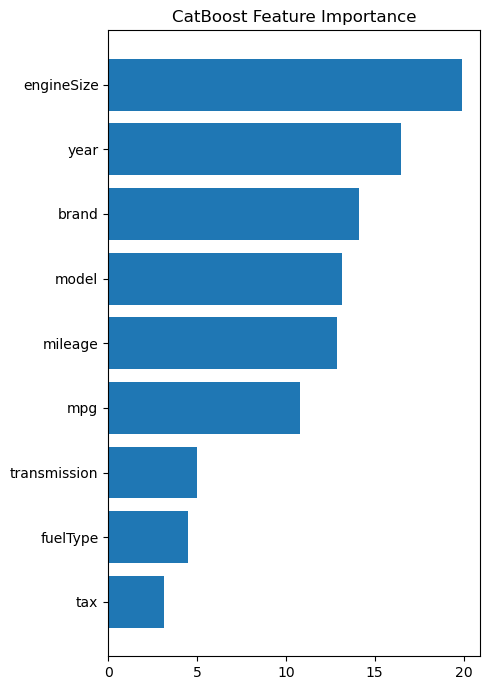
\includegraphics[keepaspectratio]{LightGBM_CatBoost_files/figure-pdf/cell-13-output-3.png}}

Check the
\href{https://catboost.ai/en/docs/references/training-parameters/common}{documentation}
for hyperparameter tuning.

With proper hyperparameter tuning, CatBoost can achieve better
performance than its default settings. However, even without tuning,
CatBoost's default configuration often outperforms the default settings
of XGBoost and LightGBM, particularly on datasets with categorical
features.

\subsection{\texorpdfstring{When to Use \textbf{CatBoost} Over
\textbf{XGBoost}}{When to Use CatBoost Over XGBoost}}\label{when-to-use-catboost-over-xgboost}

\begin{itemize}
\tightlist
\item
  When your dataset is ``categorical-heavy**
\item
  \textbf{CatBoost} tends to perform well \textbf{out of the box} with
  minimal hyperparameter tuning, making it more user-friendly for quick
  experimentation or deployment\\
\item
  CatBoost's \textbf{GPU implementation} is optimized for handling
  categorical data efficiently, and can \textbf{outperform XGBoost} on
  datasets dominated by categorical variables\\
  \textgreater{} While both libraries support GPU acceleration,
  CatBoost's architecture is particularly well-suited for
  categorical-heavy tasks
\end{itemize}

\section{Handling Imbalanced Classification: XGBoost vs.~LightGBM
vs.~CatBoost}\label{handling-imbalanced-classification-xgboost-vs.-lightgbm-vs.-catboost}

Imbalanced classification occurs when one class significantly outnumbers
the other (e.g., fraud detection, disease diagnosis). Each boosting
library offers tools to address this issue:

\textbf{XGBoost}:

\begin{itemize}
\tightlist
\item
  \textbf{Parameter}: \texttt{scale\_pos\_weight}

  \begin{itemize}
  \tightlist
  \item
    Formula:\\
    \[
    \texttt{scale\_pos\_weight} = \frac{\text{Number of negative samples}}{\text{Number of positive samples}}
    \]
  \item
    Increases the gradient of the positive class during training.
  \end{itemize}
\item
  \textbf{Additional Strategies}:

  \begin{itemize}
  \tightlist
  \item
    Use custom \texttt{eval\_metric} (e.g., \texttt{"auc"},
    \texttt{"aucpr"}, or \texttt{"logloss"})
  \item
    Apply early stopping on validation AUC
  \end{itemize}
\end{itemize}

\textbf{LightGBM}:

\begin{itemize}
\tightlist
\item
  \textbf{Parameter}: \texttt{scale\_pos\_weight} (same as in XGBoost)
\item
  \textbf{Alternative}: \texttt{is\_unbalance\ =\ TRUE}

  \begin{itemize}
  \tightlist
  \item
    Automatically adjusts class weights based on distribution
  \end{itemize}
\item
  \textbf{Other Tips}:

  \begin{itemize}
  \tightlist
  \item
    Use \texttt{metric\ =\ "auc"} or \texttt{"binary\_logloss"} for
    better guidance during training
  \item
    Resampling techniques also compatible
  \end{itemize}
\end{itemize}

\textbf{CatBoost}:

\begin{itemize}
\tightlist
\item
  \textbf{Parameter}: \texttt{class\_weights}

  \begin{itemize}
  \tightlist
  \item
    Accepts a numeric vector (e.g., \texttt{class\_weights\ =\ c(1,\ 5)}
    for {[}negative, positive{]})
  \item
    Directly modifies the loss function to emphasize minority class
  \end{itemize}
\item
  \textbf{Advantages}:

  \begin{itemize}
  \tightlist
  \item
    More flexible than \texttt{scale\_pos\_weight}
  \item
    Works well with default settings
  \end{itemize}
\item
  \textbf{Other Tips}:

  \begin{itemize}
  \tightlist
  \item
    Use \texttt{loss\_function\ =\ "Logloss"} and
    \texttt{eval\_metric\ =\ "AUC"} for binary classification
  \end{itemize}
\end{itemize}

Below is the summary table:

\begin{longtable}[]{@{}
  >{\raggedright\arraybackslash}p{(\linewidth - 6\tabcolsep) * \real{0.1048}}
  >{\raggedright\arraybackslash}p{(\linewidth - 6\tabcolsep) * \real{0.3810}}
  >{\raggedright\arraybackslash}p{(\linewidth - 6\tabcolsep) * \real{0.2381}}
  >{\raggedright\arraybackslash}p{(\linewidth - 6\tabcolsep) * \real{0.2762}}@{}}
\toprule\noalign{}
\begin{minipage}[b]{\linewidth}\raggedright
Library
\end{minipage} & \begin{minipage}[b]{\linewidth}\raggedright
Imbalance Handling Parameter
\end{minipage} & \begin{minipage}[b]{\linewidth}\raggedright
Default Support
\end{minipage} & \begin{minipage}[b]{\linewidth}\raggedright
Recommended Metric
\end{minipage} \\
\midrule\noalign{}
\endhead
\bottomrule\noalign{}
\endlastfoot
XGBoost & \texttt{scale\_pos\_weight} & No & \texttt{auc},
\texttt{aucpr} \\
LightGBM & \texttt{scale\_pos\_weight}, \texttt{is\_unbalance} & Yes
(with flag) & \texttt{auc}, \texttt{binary\_logloss} \\
CatBoost & \texttt{class\_weights} & Yes & \texttt{Logloss},
\texttt{AUC} \\
\end{longtable}

\section{Summary: XGBoost vs.~LightGBM
vs.~CatBoost}\label{summary-xgboost-vs.-lightgbm-vs.-catboost}

Gradient boosting is a powerful ensemble technique, and XGBoost,
LightGBM, and CatBoost are three of its most widely used
implementations. Each has unique strengths and is well-suited to
different use cases.

\textbf{XGBoost}:

\begin{itemize}
\tightlist
\item
  \textbf{Strengths}: Robust, well-documented, strong performance on
  structured/tabular data\\
\item
  \textbf{Split Finding}: Level-wise tree growth\\
\item
  \textbf{Regularization}: Explicit L1 and L2 regularization\\
\item
  \textbf{Flexibility}: Highly customizable with many hyperparameters\\
\item
  \textbf{Best for}: General-purpose tabular data, especially when you
  have time to tune parameters
\end{itemize}

\textbf{LightGBM}:

\begin{itemize}
\tightlist
\item
  \textbf{Strengths}: Fast training, low memory usage, excellent
  scalability\\
\item
  \textbf{Split Finding}: Leaf-wise tree growth with depth control\\
\item
  \textbf{Binning}: Uses histogram-based algorithm with
  \texttt{max\_bin} to speed up training\\
\item
  \textbf{Best for}: Large-scale datasets, high-dimensional features,
  and when training speed matters
\end{itemize}

\textbf{CatBoost}:

\begin{itemize}
\tightlist
\item
  \textbf{Strengths}: Handles categorical features natively, works well
  with minimal tuning\\
\item
  \textbf{Boosting Innovation}: Uses \emph{ordered boosting} to prevent
  prediction shift\\
\item
  \textbf{Categorical Encoding}: Uses target-based encoding internally\\
\item
  \textbf{Best for}: Datasets with many categorical variables or limited
  time for tuning
\end{itemize}

\textbf{Final Thoughts}

All three libraries are powerful and battle-tested. Here's a rough
guideline:

\begin{itemize}
\tightlist
\item
  \textbf{Use XGBoost} if you want control, flexibility, and a
  well-documented standard
\item
  \textbf{Use LightGBM} when training speed and large data scalability
  are your top priorities
\item
  \textbf{Use CatBoost} when working with many categorical features or
  seeking strong baseline results with minimal tuning
\end{itemize}

\section{References}\label{references}

\begin{itemize}
\tightlist
\item
  \href{https://papers.nips.cc/paper_files/paper/2017/file/6449f44a102fde848669bdd9eb6b76fa-Paper.pdf}{LightGBM
  Paper (Original NIPS 2017)}
\item
  \href{https://lightgbm.readthedocs.io/}{LightGBM Official Website}
\item
  \href{https://arxiv.org/abs/1810.11363}{CatBoost Paper (arXiv)}
\item
  \href{https://catboost.ai/}{CatBoost Official Website}
\end{itemize}

\chapter{Smarter Hyperparameter Optimization for Tree-Based
Models}\label{smarter-hyperparameter-optimization-for-tree-based-models}

Tree-based models, like decision trees, random forests, and boosting
algorithms (e.g., XGBoost, LightGBM, CatBoost), benefit significantly
from hyperparameter optimization. Tools like \texttt{GridSearchCV},
\texttt{RandomizedSearchCV}, and \texttt{cross\_val\_score} in
scikit-learn enable robust tuning via cross-validation, similar to
linear or logistic regression models. Below, we explore these tools and
smarter alternatives for complex models.

\section{Cross-Validation Basics}\label{cross-validation-basics}

\begin{itemize}
\item
  \texttt{cross\_val\_score}: Evaluates a model's performance for a
  fixed set of hyperparameters using cross-validation. Requires manual
  loops to search over hyperparameter combinations, making it
  labor-intensive for extensive tuning.
\item
  \texttt{GridSearchCV} and \texttt{RandomizedSearchCV}: Automate
  hyperparameter search with built-in cross-validation, internally
  handling loops to evaluate combinations efficiently.
\end{itemize}

\section{\texorpdfstring{\texttt{GridSearchCV}: Exhaustive but
Limited}{GridSearchCV: Exhaustive but Limited}}\label{gridsearchcv-exhaustive-but-limited}

\texttt{GridSearchCV} performs an \textbf{exhaustive search} over a
predefined grid of hyperparameter values.

\begin{itemize}
\tightlist
\item
  \textbf{Pros}:

  \begin{itemize}
  \tightlist
  \item
    Guarantees finding the best combination within the specified grid.
  \item
    Ideal for small, well-defined search spaces (e.g., tuning
    \texttt{max\_depth={[}3,\ 5,\ 7{]}} and
    \texttt{n\_estimators={[}100,\ 200{]}}).
  \end{itemize}
\item
  \textbf{Cons}:

  \begin{itemize}
  \tightlist
  \item
    Requires \textbf{discrete lists} for each hyperparameter, unable to
    sample from continuous distributions.
  \item
    Grid size grows \textbf{exponentially} with more hyperparameters,
    making it \textbf{computationally infeasible} for complex models
    like boosting trees (e.g., XGBoost with 5+ hyperparameters).
  \item
    Time-consuming, especially for large datasets or slow models.
  \end{itemize}
\end{itemize}

\textbf{Use Case}: Best for simple models or when you have a small,
targeted set of hyperparameter values.

\section{\texorpdfstring{\texttt{RandomizedSearchCV}: Efficient but
Random}{RandomizedSearchCV: Efficient but Random}}\label{randomizedsearchcv-efficient-but-random}

\texttt{RandomizedSearchCV} samples a fixed number of hyperparameter
combinations (\texttt{n\_iter}) randomly from user-defined
distributions.

\begin{itemize}
\tightlist
\item
  \textbf{Pros}:

  \begin{itemize}
  \item
    \textbf{More efficient} than \texttt{GridSearchCV} for large search
    spaces, as it evaluates fewer combinations.
  \item
    Supports \textbf{continuous distributions} (e.g.,
    \texttt{scipy.stats.loguniform} for learning rate), offering greater
    flexibility.

\begin{Shaded}
\begin{Highlighting}[]
\ImportTok{from}\NormalTok{ scipy.stats }\ImportTok{import}\NormalTok{ uniform}
\CommentTok{\textquotesingle{}learning\_rate\textquotesingle{}}\NormalTok{: uniform(loc}\OperatorTok{=}\FloatTok{0.01}\NormalTok{, scale}\OperatorTok{=}\FloatTok{0.3}\NormalTok{),  }\CommentTok{\# Range: [0.01, 0.31)}
\end{Highlighting}
\end{Shaded}
  \item
    \textbf{Faster}, as it avoids exhaustive enumeration.
  \end{itemize}
\item
  \textbf{Cons}:

  \begin{itemize}
  \tightlist
  \item
    Random sampling may \textbf{miss optimal regions}, especially in
    high-dimensional spaces or with limited iterations.
  \item
    Performance depends on the choice of \texttt{n\_iter} and
    distribution quality.
  \end{itemize}
\end{itemize}

\textbf{Use Case}: Preferred for \textbf{initial exploration} or when
\textbf{computational resources are limited} but the search space is
large.

\section{Challenges with Boosting
Models}\label{challenges-with-boosting-models}

Boosting models (e.g., Gradient Boosting, XGBoost, LightGBM) are
powerful but have \textbf{many hyperparameters} (e.g., learning rate,
max depth, number of estimators, regularization terms). This complexity
makes \texttt{GridSearchCV} impractical and \texttt{RandomizedSearchCV}
suboptimal, as random sampling can be inefficient in high-dimensional
spaces.

\section{Smarter Alternatives for Complex
Models}\label{smarter-alternatives-for-complex-models}

For boosting models, neural networks, or other high-dimensional
algorithms, intelligent optimization methods outperform traditional
approaches by efficiently exploring the hyperparameter space. Here are
the top alternatives:

\subsection{\texorpdfstring{1. \texttt{BayesSearchCV} (Bayesian
Optimization)}{1. BayesSearchCV (Bayesian Optimization)}}\label{bayessearchcv-bayesian-optimization}

\begin{itemize}
\item
  \textbf{How it works}: Uses a probabilistic surrogate model (e.g.,
  Gaussian Process) to predict promising hyperparameter combinations
  based on past evaluations.
\item
  \textbf{Advantages}:

  \begin{itemize}
  \tightlist
  \item
    Converges faster than random search by focusing on high-performing
    regions.
  \item
    It works natively with scikit-learn pipelines, simplifying tuning
    for workflows with preprocessing
  \item
    GP (Gassian Process) - based optimization is effective for smooth,
    continuous hyperparameters (e.g., learning rate, regularization),
    converging faster in low-dimensional spaces (Tuning 2-5 continuous
    parameters).
  \item
    Ideal for produnction environment restricted to scikit-learn
    extensions
  \end{itemize}
\item
  \textbf{Library}: \texttt{scikit-optimize} or \texttt{bayes\_opt}.
\item
  \textbf{Use Case}: Ideal for \textbf{small to medium} search spaces
  with \textbf{continuous parameters} on \textbf{small to medium-sized}
  datasets.
\end{itemize}

\begin{Shaded}
\begin{Highlighting}[]
\ImportTok{import}\NormalTok{ pandas }\ImportTok{as}\NormalTok{ pd}
\ImportTok{import}\NormalTok{ numpy }\ImportTok{as}\NormalTok{ np}
\ImportTok{import}\NormalTok{ matplotlib.pyplot }\ImportTok{as}\NormalTok{ plt}
\ImportTok{from}\NormalTok{ sklearn.model\_selection }\ImportTok{import}\NormalTok{ train\_test\_split, GridSearchCV}
\ImportTok{from}\NormalTok{ sklearn.preprocessing }\ImportTok{import}\NormalTok{ OneHotEncoder, StandardScaler}
\ImportTok{from}\NormalTok{ sklearn.compose }\ImportTok{import}\NormalTok{ ColumnTransformer}
\ImportTok{from}\NormalTok{ sklearn.pipeline }\ImportTok{import}\NormalTok{ Pipeline}
\ImportTok{from}\NormalTok{ sklearn.metrics }\ImportTok{import}\NormalTok{ root\_mean\_squared\_error, r2\_score, accuracy\_score, precision\_score, recall\_score, f1\_score, precision\_recall\_curve}
\ImportTok{from}\NormalTok{ xgboost }\ImportTok{import}\NormalTok{ XGBRegressor, XGBClassifier}
\ImportTok{import}\NormalTok{ seaborn }\ImportTok{as}\NormalTok{ sns}
\ImportTok{import}\NormalTok{ plotly}

\ImportTok{from}\NormalTok{ skopt }\ImportTok{import}\NormalTok{ BayesSearchCV}
\ImportTok{from}\NormalTok{ skopt.space }\ImportTok{import}\NormalTok{ Real, Categorical, Integer}
\ImportTok{from}\NormalTok{ skopt.plots }\ImportTok{import}\NormalTok{ plot\_objective, plot\_histogram, plot\_convergence}
\ImportTok{import}\NormalTok{ warnings}
\ImportTok{from}\NormalTok{ IPython }\ImportTok{import}\NormalTok{ display}
\end{Highlighting}
\end{Shaded}

\begin{Shaded}
\begin{Highlighting}[]
\CommentTok{\# Load the dataset}
\NormalTok{car }\OperatorTok{=}\NormalTok{ pd.read\_csv(}\StringTok{\textquotesingle{}Datasets/car.csv\textquotesingle{}}\NormalTok{)}
\NormalTok{car.head()}
\end{Highlighting}
\end{Shaded}

\begin{longtable}[]{@{}lllllllllll@{}}
\toprule\noalign{}
& brand & model & year & transmission & mileage & fuelType & tax & mpg &
engineSize & price \\
\midrule\noalign{}
\endhead
\bottomrule\noalign{}
\endlastfoot
0 & vw & Beetle & 2014 & Manual & 55457 & Diesel & 30 & 65.3266 & 1.6 &
7490 \\
1 & vauxhall & GTC & 2017 & Manual & 15630 & Petrol & 145 & 47.2049 &
1.4 & 10998 \\
2 & merc & G Class & 2012 & Automatic & 43000 & Diesel & 570 & 25.1172 &
3.0 & 44990 \\
3 & audi & RS5 & 2019 & Automatic & 10 & Petrol & 145 & 30.5593 & 2.9 &
51990 \\
4 & merc & X-CLASS & 2018 & Automatic & 14000 & Diesel & 240 & 35.7168 &
2.3 & 28990 \\
\end{longtable}

\begin{Shaded}
\begin{Highlighting}[]
\NormalTok{X }\OperatorTok{=}\NormalTok{ car.drop(columns}\OperatorTok{=}\NormalTok{[}\StringTok{\textquotesingle{}price\textquotesingle{}}\NormalTok{])}
\NormalTok{y }\OperatorTok{=}\NormalTok{ car[}\StringTok{\textquotesingle{}price\textquotesingle{}}\NormalTok{]}

\CommentTok{\# extract the categorical columns and put them in a list}
\NormalTok{categorical\_feature }\OperatorTok{=}\NormalTok{ X.select\_dtypes(include}\OperatorTok{=}\NormalTok{[}\StringTok{\textquotesingle{}object\textquotesingle{}}\NormalTok{]).columns.tolist()}

\CommentTok{\# extract the numerical columns and put them in a list}
\NormalTok{numerical\_feature }\OperatorTok{=}\NormalTok{ X.select\_dtypes(include}\OperatorTok{=}\NormalTok{[}\StringTok{\textquotesingle{}int64\textquotesingle{}}\NormalTok{, }\StringTok{\textquotesingle{}float64\textquotesingle{}}\NormalTok{]).columns.tolist()}

\CommentTok{\# convert the categorical columns to category type}
\ControlFlowTok{for}\NormalTok{ col }\KeywordTok{in}\NormalTok{ categorical\_feature:}
\NormalTok{    X[col] }\OperatorTok{=}\NormalTok{ X[col].astype(}\StringTok{\textquotesingle{}category\textquotesingle{}}\NormalTok{)}


\CommentTok{\# Split the data into training and testing sets}
\NormalTok{X\_train, X\_test, y\_train, y\_test }\OperatorTok{=}\NormalTok{ train\_test\_split(X, y, test\_size}\OperatorTok{=}\FloatTok{0.2}\NormalTok{, random\_state}\OperatorTok{=}\DecValTok{42}\NormalTok{)}
\end{Highlighting}
\end{Shaded}

\begin{Shaded}
\begin{Highlighting}[]
\CommentTok{\# build a baseline xgboost model}
\NormalTok{xgb }\OperatorTok{=}\NormalTok{ XGBRegressor(objective}\OperatorTok{=}\StringTok{\textquotesingle{}reg:squarederror\textquotesingle{}}\NormalTok{, enable\_categorical}\OperatorTok{=}\VariableTok{True}\NormalTok{, random\_state}\OperatorTok{=}\DecValTok{42}\NormalTok{)}
\CommentTok{\# fit the model}
\NormalTok{xgb.fit(X\_train, y\_train, )}
\CommentTok{\# make predictions}
\NormalTok{y\_pred }\OperatorTok{=}\NormalTok{ xgb.predict(X\_test)}

\BuiltInTok{print}\NormalTok{ (}\StringTok{\textquotesingle{}Baseline Model: \textquotesingle{}}\NormalTok{)}
\CommentTok{\# calculate the RMSE}
\NormalTok{rmse }\OperatorTok{=}\NormalTok{ root\_mean\_squared\_error(y\_test, y\_pred)}
\BuiltInTok{print}\NormalTok{(}\SpecialStringTok{f\textquotesingle{}RMSE: }\SpecialCharTok{\{}\NormalTok{rmse}\SpecialCharTok{\}}\SpecialStringTok{\textquotesingle{}}\NormalTok{)}
\CommentTok{\# calculate the R2 score}
\NormalTok{r2 }\OperatorTok{=}\NormalTok{ r2\_score(y\_test, y\_pred)}
\BuiltInTok{print}\NormalTok{(}\SpecialStringTok{f\textquotesingle{}R2: }\SpecialCharTok{\{}\NormalTok{r2}\SpecialCharTok{\}}\SpecialStringTok{\textquotesingle{}}\NormalTok{)}
\end{Highlighting}
\end{Shaded}

\begin{verbatim}
Baseline Model: 
RMSE: 3299.648193359375
R2: 0.9628884792327881
\end{verbatim}

Let's use BayesSearchCV to boost its performance

\begin{Shaded}
\begin{Highlighting}[]
\OperatorTok{\%\%}\NormalTok{time}
\CommentTok{\# define the search space for Bayesian optimization}
\NormalTok{search\_space }\OperatorTok{=}\NormalTok{ \{}
    \StringTok{\textquotesingle{}n\_estimators\textquotesingle{}}\NormalTok{: Integer(}\DecValTok{50}\NormalTok{, }\DecValTok{500}\NormalTok{),}
    \StringTok{\textquotesingle{}max\_depth\textquotesingle{}}\NormalTok{: Integer(}\DecValTok{5}\NormalTok{, }\DecValTok{30}\NormalTok{),}
    \StringTok{\textquotesingle{}learning\_rate\textquotesingle{}}\NormalTok{: Real(}\FloatTok{0.01}\NormalTok{, }\FloatTok{0.3}\NormalTok{, prior}\OperatorTok{=}\StringTok{\textquotesingle{}uniform\textquotesingle{}}\NormalTok{),}
    \StringTok{\textquotesingle{}subsample\textquotesingle{}}\NormalTok{: Real(}\FloatTok{0.5}\NormalTok{, }\FloatTok{1.0}\NormalTok{, prior}\OperatorTok{=}\StringTok{\textquotesingle{}uniform\textquotesingle{}}\NormalTok{),}
    \StringTok{\textquotesingle{}colsample\_bytree\textquotesingle{}}\NormalTok{: Real(}\FloatTok{0.5}\NormalTok{, }\FloatTok{1.0}\NormalTok{, prior}\OperatorTok{=}\StringTok{\textquotesingle{}uniform\textquotesingle{}}\NormalTok{),}
    \StringTok{\textquotesingle{}gamma\textquotesingle{}}\NormalTok{: Real(}\DecValTok{0}\NormalTok{, }\DecValTok{5}\NormalTok{, prior}\OperatorTok{=}\StringTok{\textquotesingle{}uniform\textquotesingle{}}\NormalTok{),}
\NormalTok{\}}

\CommentTok{\# define the model}
\NormalTok{xgb }\OperatorTok{=}\NormalTok{ XGBRegressor(objective}\OperatorTok{=}\StringTok{\textquotesingle{}reg:squarederror\textquotesingle{}}\NormalTok{, enable\_categorical}\OperatorTok{=}\VariableTok{True}\NormalTok{, random\_state}\OperatorTok{=}\DecValTok{42}\NormalTok{)}
\CommentTok{\# define the Bayesian optimization search}
\NormalTok{bayes\_search }\OperatorTok{=}\NormalTok{ BayesSearchCV(}
\NormalTok{    xgb,}
\NormalTok{    search\_space,}
\NormalTok{    n\_iter}\OperatorTok{=}\DecValTok{50}\NormalTok{,}
\NormalTok{    scoring}\OperatorTok{=}\StringTok{\textquotesingle{}neg\_root\_mean\_squared\_error\textquotesingle{}}\NormalTok{,}
\NormalTok{    cv}\OperatorTok{=}\DecValTok{3}\NormalTok{,}
\NormalTok{    n\_jobs}\OperatorTok{={-}}\DecValTok{1}\NormalTok{,}
\NormalTok{    random\_state}\OperatorTok{=}\DecValTok{42}\NormalTok{,}
\NormalTok{    verbose}\OperatorTok{=}\DecValTok{0}
\NormalTok{)}
\CommentTok{\# fit the model}
\NormalTok{bayes\_search.fit(X\_train, y\_train)}
\end{Highlighting}
\end{Shaded}

\begin{verbatim}
CPU times: total: 46.6 s
Wall time: 3min 24s
\end{verbatim}

\begin{verbatim}
BayesSearchCV(cv=3,
              estimator=XGBRegressor(base_score=None, booster=None,
                                     callbacks=None, colsample_bylevel=None,
                                     colsample_bynode=None,
                                     colsample_bytree=None, device=None,
                                     early_stopping_rounds=None,
                                     enable_categorical=True, eval_metric=None,
                                     feature_types=None, feature_weights=None,
                                     gamma=None, grow_policy=None,
                                     importance_type=None,
                                     interaction_constraints=None...
                             'gamma': Real(low=0, high=5, prior='uniform', transform='normalize'),
                             'learning_rate': Real(low=0.01, high=0.3, prior='uniform', transform='normalize'),
                             'max_depth': Integer(low=5, high=30, prior='uniform', transform='normalize'),
                             'n_estimators': Integer(low=50, high=500, prior='uniform', transform='normalize'),
                             'subsample': Real(low=0.5, high=1.0, prior='uniform', transform='normalize')})
\end{verbatim}

\begin{Shaded}
\begin{Highlighting}[]
\BuiltInTok{print}\NormalTok{(}\StringTok{\textquotesingle{}Bayesian Optimization Results: \textquotesingle{}}\NormalTok{)}
\CommentTok{\# get the best parameters}
\NormalTok{best\_params\_bayes }\OperatorTok{=}\NormalTok{ bayes\_search.best\_params\_}
\BuiltInTok{print}\NormalTok{(}\StringTok{\textquotesingle{}Best Parameters: \textquotesingle{}}\NormalTok{)}
\BuiltInTok{print}\NormalTok{(best\_params\_bayes)}
\CommentTok{\# get the best score}
\NormalTok{best\_score\_bayes }\OperatorTok{=}\NormalTok{ bayes\_search.best\_score\_}
\BuiltInTok{print}\NormalTok{(}\StringTok{\textquotesingle{}Best CV Score: \textquotesingle{}}\NormalTok{, best\_score\_bayes)}
\CommentTok{\# make predictions}
\NormalTok{y\_pred\_bayes }\OperatorTok{=}\NormalTok{ bayes\_search.predict(X\_test)}
\CommentTok{\# calculate the RMSE}
\NormalTok{rmse\_bayes }\OperatorTok{=}\NormalTok{ root\_mean\_squared\_error(y\_test, y\_pred\_bayes)}
\BuiltInTok{print}\NormalTok{(}\StringTok{\textquotesingle{}Test RMSE: \textquotesingle{}}\NormalTok{, rmse\_bayes)}
\CommentTok{\# calculate the R2 score}
\NormalTok{r2\_bayes }\OperatorTok{=}\NormalTok{ r2\_score(y\_test, y\_pred\_bayes)}
\BuiltInTok{print}\NormalTok{(}\StringTok{\textquotesingle{}Test R2: \textquotesingle{}}\NormalTok{, r2\_bayes)}

\end{Highlighting}
\end{Shaded}

\begin{verbatim}
Bayesian Optimization Results: 
Best Parameters: 
OrderedDict({'colsample_bytree': 0.7800962787418171, 'gamma': 5.0, 'learning_rate': 0.03253670126492928, 'max_depth': 5, 'n_estimators': 342, 'subsample': 0.5})
Best CV Score:  -3061.9464518229165
Test RMSE:  3236.476318359375
Test R2:  0.9642958641052246
\end{verbatim}

\subsection{\texorpdfstring{Visualizing \texttt{BayesSearchCV}
Results}{Visualizing BayesSearchCV Results}}\label{visualizing-bayessearchcv-results}

Visualizing \texttt{BayesSearchCV} outcomes helps interpret the
hyperparameter optimization process for tree-based models like
\textbf{XGBoost}. Visualization can provide critical insights into
convergence, parameter impact, and model behavior, helping you
understand and refine model behavior.

\textbf{Key Benefits of Visualization:}

\begin{itemize}
\item
  \textbf{Check Convergence}:\\
  Plot best scores vs.~iterations to determine if the search has
  stabilized or requires more trials.
\item
  \textbf{Identify Key Parameters}:\\
  Use scatter plots to reveal which hyperparameters (e.g.,
  \texttt{learning\_rate}) significantly influence performance.
\item
  \textbf{Explore Interactions}:\\
  Use heatmaps or contour plots to examine relationships between
  hyperparameters (e.g., \texttt{learning\_rate}
  vs.~\texttt{max\_depth}).
\item
  \textbf{Diagnose Issues}:\\
  Spot poor search regions or insufficient iterations through patterns
  in the plots.
\end{itemize}

\textbf{Practical Tips}

\begin{itemize}
\item
  \textbf{Plots}:\\
  Use convergence, scatter, heatmap, or parallel coordinate plots with
  libraries like \textbf{Matplotlib} or \textbf{Seaborn}.
\item
  \textbf{Accessing Results}:\\
  Extract tuning history from the \texttt{cv\_results\_} attribute of
  the \texttt{BayesSearchCV} object for plotting.
\end{itemize}

Let's plot the convergence first

\begin{Shaded}
\begin{Highlighting}[]
\ImportTok{from}\NormalTok{ skopt.plots }\ImportTok{import}\NormalTok{ plot\_convergence, plot\_objective}

\CommentTok{\# plot the convergence}
\NormalTok{bayes\_res }\OperatorTok{=}\NormalTok{ bayes\_search.optimizer\_results\_[}\DecValTok{0}\NormalTok{]}
\NormalTok{plot\_convergence(bayes\_res)}
\NormalTok{plt.show()}
\end{Highlighting}
\end{Shaded}

\pandocbounded{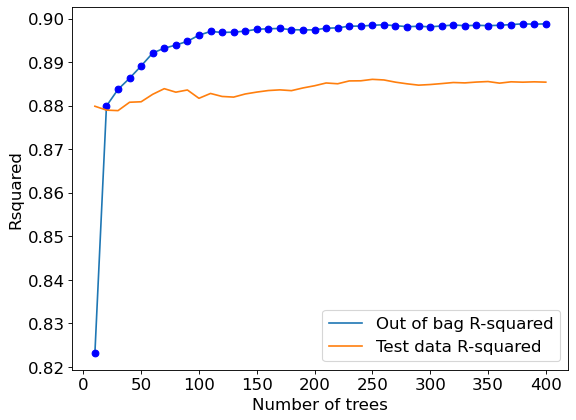
\includegraphics[keepaspectratio]{smarter_hyper_tuning_files/figure-pdf/cell-8-output-1.png}}

\begin{Shaded}
\begin{Highlighting}[]
\CommentTok{\# the raw objective values at each iteration}
\NormalTok{func\_vals }\OperatorTok{=}\NormalTok{ np.array(bayes\_res.func\_vals)}

\CommentTok{\# the best objective value found so far}
\NormalTok{best\_val }\OperatorTok{=}\NormalTok{ func\_vals.}\BuiltInTok{min}\NormalTok{()}

\CommentTok{\# All iterations (1{-}based) that hit that minimum}
\NormalTok{best\_iters }\OperatorTok{=}\NormalTok{ np.where(func\_vals }\OperatorTok{==}\NormalTok{ best\_val)[}\DecValTok{0}\NormalTok{] }\OperatorTok{+} \DecValTok{1}

\BuiltInTok{print}\NormalTok{(}\SpecialStringTok{f"Best objective = }\SpecialCharTok{\{}\NormalTok{best\_val}\SpecialCharTok{:.4f\}}\SpecialStringTok{"}\NormalTok{)}
\BuiltInTok{print}\NormalTok{(}\SpecialStringTok{f"Reached at iteration(s): }\SpecialCharTok{\{}\NormalTok{best\_iters}\SpecialCharTok{.}\NormalTok{tolist()}\SpecialCharTok{\}}\SpecialStringTok{"}\NormalTok{)}
\end{Highlighting}
\end{Shaded}

\begin{verbatim}
Best objective = 3061.9465
Reached at iteration(s): [50]
\end{verbatim}

\begin{itemize}
\item
  \texttt{func\_vals} is an array of length \texttt{n\_iter}, one entry
  per call.
\item
  We use \texttt{argmin/min} because by default BayesSearchCV minimizes
  the underlying surrogate objective (here negative MAE).
\item
  If you're maximizing some metric, either negate func\_vals or look at
  -best\_val appropriately.
\end{itemize}

Let's plot the objective next

\begin{Shaded}
\begin{Highlighting}[]
\CommentTok{\# Plot and store the figure and axes}
\NormalTok{fig, ax }\OperatorTok{=}\NormalTok{ plt.subplots(figsize}\OperatorTok{=}\NormalTok{(}\DecValTok{14}\NormalTok{, }\DecValTok{8}\NormalTok{))}
\NormalTok{result }\OperatorTok{=}\NormalTok{ plot\_objective(bayes\_search.optimizer\_results\_[}\DecValTok{0}\NormalTok{], ax}\OperatorTok{=}\NormalTok{ax)}

\CommentTok{\# Find contour plots in all the axes}
\ControlFlowTok{for}\NormalTok{ i, ax }\KeywordTok{in} \BuiltInTok{enumerate}\NormalTok{(fig.get\_axes()):}
    \CommentTok{\# Look for collections in each axis}
    \ControlFlowTok{for}\NormalTok{ collection }\KeywordTok{in}\NormalTok{ ax.collections:}
        \ControlFlowTok{if} \BuiltInTok{isinstance}\NormalTok{(collection, plt.matplotlib.collections.QuadMesh) }\KeywordTok{or} \OperatorTok{\textbackslash{}}
           \BuiltInTok{isinstance}\NormalTok{(collection, plt.matplotlib.collections.PathCollection):}
            \CommentTok{\# Add colorbar for this collection}
\NormalTok{            cbar }\OperatorTok{=}\NormalTok{ fig.colorbar(collection, ax}\OperatorTok{=}\NormalTok{ax)}
\NormalTok{            cbar.set\_label(}\StringTok{\textquotesingle{}Objective Value\textquotesingle{}}\NormalTok{)}
            \ControlFlowTok{break}

\NormalTok{plt.tight\_layout()}
\NormalTok{plt.show()}
\end{Highlighting}
\end{Shaded}

\pandocbounded{\includegraphics[keepaspectratio]{smarter_hyper_tuning_files/figure-pdf/cell-10-output-1.png}}

Let's plot evalutions next

\begin{Shaded}
\begin{Highlighting}[]
\ImportTok{from}\NormalTok{ skopt.plots }\ImportTok{import}\NormalTok{ plot\_evaluations}

\NormalTok{plot\_evaluations(bayes\_search.optimizer\_results\_[}\DecValTok{0}\NormalTok{], bins}\OperatorTok{=}\DecValTok{10}\NormalTok{)}
\NormalTok{plt.show()}
\end{Highlighting}
\end{Shaded}

\pandocbounded{\includegraphics[keepaspectratio]{smarter_hyper_tuning_files/figure-pdf/cell-11-output-1.png}}

Let's visualize parameter distributions next

\begin{Shaded}
\begin{Highlighting}[]
\CommentTok{\# Get hyperparameter names from BayesSearchCV\textquotesingle{}s search\_spaces}
\NormalTok{results }\OperatorTok{=}\NormalTok{ bayes\_search.cv\_results\_}
\NormalTok{best\_params }\OperatorTok{=}\NormalTok{ bayes\_search.best\_params\_}

\CommentTok{\# Convert results to DataFrame}
\NormalTok{results\_df }\OperatorTok{=}\NormalTok{ pd.DataFrame(results)}

\CommentTok{\# Create plots for each parameter}
\NormalTok{fig, axes }\OperatorTok{=}\NormalTok{ plt.subplots(}\DecValTok{1}\NormalTok{, }\BuiltInTok{len}\NormalTok{(best\_params), figsize}\OperatorTok{=}\NormalTok{(}\DecValTok{15}\NormalTok{, }\DecValTok{4}\NormalTok{))}
\NormalTok{params }\OperatorTok{=} \BuiltInTok{list}\NormalTok{(best\_params.keys())}

\ControlFlowTok{for}\NormalTok{ i, param }\KeywordTok{in} \BuiltInTok{enumerate}\NormalTok{(params):}
\NormalTok{    param\_name }\OperatorTok{=} \SpecialStringTok{f\textquotesingle{}param\_}\SpecialCharTok{\{}\NormalTok{param}\SpecialCharTok{\}}\SpecialStringTok{\textquotesingle{}}
    \CommentTok{\# Extract parameter values}
\NormalTok{    param\_values }\OperatorTok{=}\NormalTok{ results\_df[param\_name].values}
    
    \CommentTok{\# Scatter plot: parameter value vs performance}
\NormalTok{    axes[i].scatter(param\_values, results\_df[}\StringTok{\textquotesingle{}mean\_test\_score\textquotesingle{}}\NormalTok{])}
\NormalTok{    axes[i].set\_xlabel(param)}
\NormalTok{    axes[i].set\_ylabel(}\StringTok{\textquotesingle{}Mean Test Score\textquotesingle{}}\NormalTok{)}
\NormalTok{    axes[i].axvline(best\_params[param], color}\OperatorTok{=}\StringTok{\textquotesingle{}r\textquotesingle{}}\NormalTok{, linestyle}\OperatorTok{=}\StringTok{\textquotesingle{}{-}{-}\textquotesingle{}}\NormalTok{, label}\OperatorTok{=}\StringTok{\textquotesingle{}Best value\textquotesingle{}}\NormalTok{)}
\NormalTok{    axes[i].legend()}

\NormalTok{plt.tight\_layout()}
\NormalTok{plt.show()}
\end{Highlighting}
\end{Shaded}

\pandocbounded{\includegraphics[keepaspectratio]{smarter_hyper_tuning_files/figure-pdf/cell-12-output-1.png}}

\subsubsection{Next Steps for Hyperparameter
Tuning}\label{next-steps-for-hyperparameter-tuning}

\textbf{Refine Search Space}

\begin{itemize}
\tightlist
\item
  Based on scatter plots, focus tuning on the most promising regions:

  \begin{itemize}
  \tightlist
  \item
    \texttt{learning\_rate}: 0.01--0.1 (red stars clustered around 0.05)
  \item
    \texttt{n\_estimators}: 50--200 (indicated by clustering and red
    stars)
  \item
    \texttt{max\_depth}: 5--15 (majority of samples fall in this range)
  \item
    \texttt{subsample}: 0.6--0.9
  \item
    \texttt{colsample\_bytree}: 0.6--0.9
  \item
    \texttt{gamma}: 0--2 (most samples are below 2)
  \end{itemize}
\item
  Narrowing the hyperparameter space \textbf{reduces computational cost}
  and concentrates the search on \textbf{high-performing regions}.
\end{itemize}

\textbf{Increase Iterations}

\begin{itemize}
\tightlist
\item
  The convergence plot suggests the search may have stabilized, but
  increasing the number of iterations (e.g., \texttt{n\_iter=75}) within
  the refined space could help confirm the optimum.
\end{itemize}

\begin{Shaded}
\begin{Highlighting}[]
\OperatorTok{\%\%}\NormalTok{time}
\CommentTok{\# refine the search space for Bayesian optimization}
\NormalTok{search\_space }\OperatorTok{=}\NormalTok{ \{}
    \StringTok{\textquotesingle{}n\_estimators\textquotesingle{}}\NormalTok{: Integer(}\DecValTok{50}\NormalTok{, }\DecValTok{500}\NormalTok{),}
    \StringTok{\textquotesingle{}max\_depth\textquotesingle{}}\NormalTok{: Integer(}\DecValTok{5}\NormalTok{, }\DecValTok{15}\NormalTok{),}
    \StringTok{\textquotesingle{}learning\_rate\textquotesingle{}}\NormalTok{: Real(}\FloatTok{0.01}\NormalTok{, }\FloatTok{0.1}\NormalTok{, prior}\OperatorTok{=}\StringTok{\textquotesingle{}uniform\textquotesingle{}}\NormalTok{),}
    \StringTok{\textquotesingle{}subsample\textquotesingle{}}\NormalTok{: Real(}\FloatTok{0.6}\NormalTok{, }\FloatTok{0.9}\NormalTok{, prior}\OperatorTok{=}\StringTok{\textquotesingle{}uniform\textquotesingle{}}\NormalTok{),}
    \StringTok{\textquotesingle{}colsample\_bytree\textquotesingle{}}\NormalTok{: Real(}\FloatTok{0.6}\NormalTok{, }\FloatTok{0.9}\NormalTok{, prior}\OperatorTok{=}\StringTok{\textquotesingle{}uniform\textquotesingle{}}\NormalTok{),}
    \StringTok{\textquotesingle{}gamma\textquotesingle{}}\NormalTok{: Real(}\DecValTok{0}\NormalTok{, }\DecValTok{2}\NormalTok{, prior}\OperatorTok{=}\StringTok{\textquotesingle{}uniform\textquotesingle{}}\NormalTok{),}
\NormalTok{\}}

\CommentTok{\# define the model}
\NormalTok{xgb }\OperatorTok{=}\NormalTok{ XGBRegressor(objective}\OperatorTok{=}\StringTok{\textquotesingle{}reg:squarederror\textquotesingle{}}\NormalTok{, enable\_categorical}\OperatorTok{=}\VariableTok{True}\NormalTok{, random\_state}\OperatorTok{=}\DecValTok{42}\NormalTok{)}
\CommentTok{\# define the Bayesian optimization search}
\NormalTok{bayes\_search }\OperatorTok{=}\NormalTok{ BayesSearchCV(}
\NormalTok{    xgb,}
\NormalTok{    search\_space,}
\NormalTok{    n\_iter}\OperatorTok{=}\DecValTok{75}\NormalTok{,}
\NormalTok{    scoring}\OperatorTok{=}\StringTok{\textquotesingle{}neg\_root\_mean\_squared\_error\textquotesingle{}}\NormalTok{,}
\NormalTok{    cv}\OperatorTok{=}\DecValTok{3}\NormalTok{,}
\NormalTok{    n\_jobs}\OperatorTok{={-}}\DecValTok{1}\NormalTok{,}
\NormalTok{    random\_state}\OperatorTok{=}\DecValTok{42}\NormalTok{,}
\NormalTok{    verbose}\OperatorTok{=}\DecValTok{0}
\NormalTok{)}
\CommentTok{\# fit the model}
\NormalTok{bayes\_search.fit(X\_train, y\_train)}
\end{Highlighting}
\end{Shaded}

\begin{verbatim}
CPU times: total: 1min 37s
Wall time: 2min 59s
\end{verbatim}

\begin{verbatim}
BayesSearchCV(cv=3,
              estimator=XGBRegressor(base_score=None, booster=None,
                                     callbacks=None, colsample_bylevel=None,
                                     colsample_bynode=None,
                                     colsample_bytree=None, device=None,
                                     early_stopping_rounds=None,
                                     enable_categorical=True, eval_metric=None,
                                     feature_types=None, feature_weights=None,
                                     gamma=None, grow_policy=None,
                                     importance_type=None,
                                     interaction_constraints=None...
                             'gamma': Real(low=0, high=2, prior='uniform', transform='normalize'),
                             'learning_rate': Real(low=0.01, high=0.1, prior='uniform', transform='normalize'),
                             'max_depth': Integer(low=5, high=15, prior='uniform', transform='normalize'),
                             'n_estimators': Integer(low=50, high=500, prior='uniform', transform='normalize'),
                             'subsample': Real(low=0.6, high=0.9, prior='uniform', transform='normalize')})
\end{verbatim}

\begin{Shaded}
\begin{Highlighting}[]
\BuiltInTok{print}\NormalTok{(}\StringTok{\textquotesingle{}Bayesian Optimization Results: \textquotesingle{}}\NormalTok{)}
\CommentTok{\# get the best parameters}
\NormalTok{best\_params\_bayes }\OperatorTok{=}\NormalTok{ bayes\_search.best\_params\_}
\BuiltInTok{print}\NormalTok{(}\StringTok{\textquotesingle{}Best Parameters: \textquotesingle{}}\NormalTok{)}
\BuiltInTok{print}\NormalTok{(best\_params\_bayes)}
\CommentTok{\# get the best score}
\NormalTok{best\_score\_bayes }\OperatorTok{=}\NormalTok{ bayes\_search.best\_score\_}
\BuiltInTok{print}\NormalTok{(}\StringTok{\textquotesingle{}Best CV Score: \textquotesingle{}}\NormalTok{, best\_score\_bayes)}
\CommentTok{\# make predictions}
\NormalTok{y\_pred\_bayes }\OperatorTok{=}\NormalTok{ bayes\_search.predict(X\_test)}
\CommentTok{\# calculate the RMSE}
\NormalTok{rmse\_bayes }\OperatorTok{=}\NormalTok{ root\_mean\_squared\_error(y\_test, y\_pred\_bayes)}
\BuiltInTok{print}\NormalTok{(}\StringTok{\textquotesingle{}Test RMSE: \textquotesingle{}}\NormalTok{, rmse\_bayes)}
\CommentTok{\# calculate the R2 score}
\NormalTok{r2\_bayes }\OperatorTok{=}\NormalTok{ r2\_score(y\_test, y\_pred\_bayes)}
\BuiltInTok{print}\NormalTok{(}\StringTok{\textquotesingle{}Test R2: \textquotesingle{}}\NormalTok{, r2\_bayes)}
\end{Highlighting}
\end{Shaded}

\begin{verbatim}
Bayesian Optimization Results: 
Best Parameters: 
OrderedDict({'colsample_bytree': 0.60000489767951, 'gamma': 1.3194686223941245, 'learning_rate': 0.024138854425252557, 'max_depth': 6, 'n_estimators': 409, 'subsample': 0.6717795261110148})
Best CV Score:  -2997.3878580729165
Test RMSE:  3131.67626953125
Test R2:  0.9665706753730774
\end{verbatim}

As can be seen, the test RMSE was further reduced after incorporating
these steps.

\begin{Shaded}
\begin{Highlighting}[]
\CommentTok{\# plot objective function}
\NormalTok{bayes\_res }\OperatorTok{=}\NormalTok{ bayes\_search.optimizer\_results\_[}\DecValTok{0}\NormalTok{]}
\NormalTok{plot\_convergence(bayes\_res)}
\NormalTok{plt.show()}
\end{Highlighting}
\end{Shaded}

\pandocbounded{\includegraphics[keepaspectratio]{smarter_hyper_tuning_files/figure-pdf/cell-15-output-1.png}}

With 75 iterations, the search appears sufficient, as the objective
value stabilizes

Alternatively, consider switching to \textbf{\texttt{Optuna}}, which
offers advanced features like \textbf{pruning}, allowing it to stop
unpromising trials early and focus computational effort on more
promising regions of the search space.

\textbf{Optuna} is often the preferred choice for tuning tree-based
models such as \textbf{XGBoost}, \textbf{LightGBM}, and
\textbf{CatBoost}, thanks to its intelligent \textbf{Tree-structured
Parzen Estimator (TPE)} search algorithm and efficient pruning strategy.

\subsection{\texorpdfstring{2. \texttt{Optuna} (Advanced TPE-Based
Optimization)}{2. Optuna (Advanced TPE-Based Optimization)}}\label{optuna-advanced-tpe-based-optimization}

\texttt{Optuna} is a modern hyperparameter optimization framework that
uses Tree-structured Parzen Estimator (TPE) and \textbf{pruning} to
efficiently explore the hyperparameter space.

\begin{itemize}
\item
  \textbf{How it works}: Models the hyperparameter space
  probabilistically and prioritizes promising combinations, stopping
  unpromising trials early (\textbf{pruning}).
\item
  \textbf{Pros}:

  \begin{itemize}
  \tightlist
  \item
    \textbf{Highly efficient} due to pruning, saving compute time for
    expensive models like boosting trees.
  \item
    Flexible, supporting dynamic search spaces and easy integration with
    XGBoost, LightGBM, and CatBoost.
  \item
    Often finds better hyperparameters with \textbf{fewer trials}
    compared to \texttt{RandomizedSearchCV}.
  \end{itemize}
\item
  \textbf{Cons}:

  \begin{itemize}
  \tightlist
  \item
    Requires slightly more setup (e.g., defining an objective function)
    than scikit-learn tools.
  \end{itemize}
\item
  \textbf{Library}: \texttt{optuna}.
\item
  \textbf{Use Case}: Best for most boosting model tasks, especially with
  \textbf{large datasets} or \textbf{complex hyperparameter spaces}.
\end{itemize}

\begin{Shaded}
\begin{Highlighting}[]
\OperatorTok{\%\%}\NormalTok{time}
\CommentTok{\# use optuna}
\ImportTok{import}\NormalTok{ optuna}
\ImportTok{from}\NormalTok{ sklearn.model\_selection }\ImportTok{import}\NormalTok{ cross\_val\_score}
\ImportTok{from}\NormalTok{ optuna }\ImportTok{import}\NormalTok{ create\_study}

\KeywordTok{def}\NormalTok{ objective(trial):}
    \CommentTok{\# Define the hyperparameters to tune}
\NormalTok{    n\_estimators }\OperatorTok{=}\NormalTok{ trial.suggest\_int(}\StringTok{\textquotesingle{}n\_estimators\textquotesingle{}}\NormalTok{, }\DecValTok{50}\NormalTok{, }\DecValTok{500}\NormalTok{)}
\NormalTok{    max\_depth }\OperatorTok{=}\NormalTok{ trial.suggest\_int(}\StringTok{\textquotesingle{}max\_depth\textquotesingle{}}\NormalTok{, }\DecValTok{5}\NormalTok{, }\DecValTok{30}\NormalTok{)}
\NormalTok{    learning\_rate }\OperatorTok{=}\NormalTok{ trial.suggest\_float(}\StringTok{\textquotesingle{}learning\_rate\textquotesingle{}}\NormalTok{, }\FloatTok{0.01}\NormalTok{, }\FloatTok{0.3}\NormalTok{)}
\NormalTok{    subsample }\OperatorTok{=}\NormalTok{ trial.suggest\_float(}\StringTok{\textquotesingle{}subsample\textquotesingle{}}\NormalTok{, }\FloatTok{0.5}\NormalTok{, }\FloatTok{1.0}\NormalTok{)}
\NormalTok{    colsample\_bytree }\OperatorTok{=}\NormalTok{ trial.suggest\_float(}\StringTok{\textquotesingle{}colsample\_bytree\textquotesingle{}}\NormalTok{, }\FloatTok{0.5}\NormalTok{, }\FloatTok{1.0}\NormalTok{)}
\NormalTok{    gamma }\OperatorTok{=}\NormalTok{ trial.suggest\_float(}\StringTok{\textquotesingle{}gamma\textquotesingle{}}\NormalTok{, }\DecValTok{0}\NormalTok{, }\DecValTok{5}\NormalTok{)}

    \CommentTok{\# Create the model}
\NormalTok{    model }\OperatorTok{=}\NormalTok{ XGBRegressor(}
\NormalTok{        n\_estimators}\OperatorTok{=}\NormalTok{n\_estimators,}
\NormalTok{        max\_depth}\OperatorTok{=}\NormalTok{max\_depth,}
\NormalTok{        learning\_rate}\OperatorTok{=}\NormalTok{learning\_rate,}
\NormalTok{        subsample}\OperatorTok{=}\NormalTok{subsample,}
\NormalTok{        colsample\_bytree}\OperatorTok{=}\NormalTok{colsample\_bytree,}
\NormalTok{        gamma}\OperatorTok{=}\NormalTok{gamma,}
\NormalTok{        objective}\OperatorTok{=}\StringTok{\textquotesingle{}reg:squarederror\textquotesingle{}}\NormalTok{,}
\NormalTok{        enable\_categorical}\OperatorTok{=}\VariableTok{True}\NormalTok{,}
\NormalTok{        random\_state}\OperatorTok{=}\DecValTok{42}
\NormalTok{    )}

    \CommentTok{\# Perform cross{-}validation}
\NormalTok{    scores }\OperatorTok{=}\NormalTok{ cross\_val\_score(model, X\_train, y\_train, cv}\OperatorTok{=}\DecValTok{3}\NormalTok{, scoring}\OperatorTok{=}\StringTok{\textquotesingle{}neg\_root\_mean\_squared\_error\textquotesingle{}}\NormalTok{)}
    
    \ControlFlowTok{return} \OperatorTok{{-}}\NormalTok{scores.mean()}

\CommentTok{\# Create a study object}
\NormalTok{study }\OperatorTok{=}\NormalTok{ create\_study(direction}\OperatorTok{=}\StringTok{\textquotesingle{}minimize\textquotesingle{}}\NormalTok{)}
\CommentTok{\# Optimize the objective function}
\NormalTok{study.optimize(objective, n\_trials}\OperatorTok{=}\DecValTok{50}\NormalTok{)}
\end{Highlighting}
\end{Shaded}

\begin{verbatim}
[I 2025-05-18 14:07:55,357] A new study created in memory with name: no-name-f3ce2686-4303-4134-ba07-01df44899c17
[I 2025-05-18 14:07:57,058] Trial 0 finished with value: 3331.6385904947915 and parameters: {'n_estimators': 110, 'max_depth': 13, 'learning_rate': 0.18884203283886744, 'subsample': 0.5854526666440897, 'colsample_bytree': 0.8937738801429804, 'gamma': 2.6946659405421385}. Best is trial 0 with value: 3331.6385904947915.
[I 2025-05-18 14:08:07,356] Trial 1 finished with value: 3532.982177734375 and parameters: {'n_estimators': 405, 'max_depth': 24, 'learning_rate': 0.16910832412869004, 'subsample': 0.9737607498458992, 'colsample_bytree': 0.5976945917277403, 'gamma': 2.817167693022663}. Best is trial 0 with value: 3331.6385904947915.
[I 2025-05-18 14:08:14,607] Trial 2 finished with value: 3277.841552734375 and parameters: {'n_estimators': 149, 'max_depth': 17, 'learning_rate': 0.04812097737053897, 'subsample': 0.9546726621457335, 'colsample_bytree': 0.8450595576069481, 'gamma': 2.3750014829760397}. Best is trial 2 with value: 3277.841552734375.
[I 2025-05-18 14:08:31,440] Trial 3 finished with value: 3288.1484375 and parameters: {'n_estimators': 239, 'max_depth': 28, 'learning_rate': 0.07547917129486585, 'subsample': 0.8139622919192127, 'colsample_bytree': 0.614390583668776, 'gamma': 4.977457905957452}. Best is trial 2 with value: 3277.841552734375.
[I 2025-05-18 14:08:33,724] Trial 4 finished with value: 3442.0733235677085 and parameters: {'n_estimators': 158, 'max_depth': 11, 'learning_rate': 0.04820580828068148, 'subsample': 0.9740363627954242, 'colsample_bytree': 0.5255147944629655, 'gamma': 3.2856067984172883}. Best is trial 2 with value: 3277.841552734375.
[I 2025-05-18 14:08:46,455] Trial 5 finished with value: 3532.2062174479165 and parameters: {'n_estimators': 427, 'max_depth': 18, 'learning_rate': 0.26452891035565, 'subsample': 0.5071558754145372, 'colsample_bytree': 0.9173489957689693, 'gamma': 4.150003935321765}. Best is trial 2 with value: 3277.841552734375.
[I 2025-05-18 14:09:01,942] Trial 6 finished with value: 3454.6267903645835 and parameters: {'n_estimators': 311, 'max_depth': 26, 'learning_rate': 0.1202287548017663, 'subsample': 0.8982432580618387, 'colsample_bytree': 0.561962457887061, 'gamma': 2.171604318548932}. Best is trial 2 with value: 3277.841552734375.
[I 2025-05-18 14:09:03,372] Trial 7 finished with value: 3168.041748046875 and parameters: {'n_estimators': 259, 'max_depth': 6, 'learning_rate': 0.15479906550009093, 'subsample': 0.722784330360674, 'colsample_bytree': 0.9717808152882963, 'gamma': 0.16914348890876785}. Best is trial 7 with value: 3168.041748046875.
[I 2025-05-18 14:09:13,799] Trial 8 finished with value: 3375.4777018229165 and parameters: {'n_estimators': 232, 'max_depth': 25, 'learning_rate': 0.24377703631670514, 'subsample': 0.7042201589884167, 'colsample_bytree': 0.7045843722953715, 'gamma': 3.672277794383117}. Best is trial 7 with value: 3168.041748046875.
[I 2025-05-18 14:09:14,891] Trial 9 finished with value: 3246.5836588541665 and parameters: {'n_estimators': 249, 'max_depth': 5, 'learning_rate': 0.24904510550714254, 'subsample': 0.5364967258658128, 'colsample_bytree': 0.870248309348203, 'gamma': 0.8871442748221514}. Best is trial 7 with value: 3168.041748046875.
[I 2025-05-18 14:09:16,406] Trial 10 finished with value: 3110.5743815104165 and parameters: {'n_estimators': 347, 'max_depth': 5, 'learning_rate': 0.12363016428276806, 'subsample': 0.6828890061277565, 'colsample_bytree': 0.9913288594327404, 'gamma': 0.028595940344607662}. Best is trial 10 with value: 3110.5743815104165.
[I 2025-05-18 14:09:17,960] Trial 11 finished with value: 3080.7557779947915 and parameters: {'n_estimators': 344, 'max_depth': 5, 'learning_rate': 0.11966202039748526, 'subsample': 0.6966666409771092, 'colsample_bytree': 0.9907568324552126, 'gamma': 0.03193020721640565}. Best is trial 11 with value: 3080.7557779947915.
[I 2025-05-18 14:09:22,688] Trial 12 finished with value: 3226.2923990885415 and parameters: {'n_estimators': 355, 'max_depth': 9, 'learning_rate': 0.11711488725389262, 'subsample': 0.631951758513077, 'colsample_bytree': 0.9983350666437509, 'gamma': 1.27168447617301}. Best is trial 11 with value: 3080.7557779947915.
[I 2025-05-18 14:09:27,330] Trial 13 finished with value: 3197.4087727864585 and parameters: {'n_estimators': 485, 'max_depth': 8, 'learning_rate': 0.10490346463062429, 'subsample': 0.8054330102331452, 'colsample_bytree': 0.7392833809068201, 'gamma': 0.0009708831636260976}. Best is trial 11 with value: 3080.7557779947915.
[I 2025-05-18 14:09:36,167] Trial 14 finished with value: 3265.5059407552085 and parameters: {'n_estimators': 350, 'max_depth': 14, 'learning_rate': 0.010974084771641884, 'subsample': 0.657436989440511, 'colsample_bytree': 0.9444260043103783, 'gamma': 1.1415074503215086}. Best is trial 11 with value: 3080.7557779947915.
[I 2025-05-18 14:09:38,021] Trial 15 finished with value: 3211.10498046875 and parameters: {'n_estimators': 414, 'max_depth': 5, 'learning_rate': 0.20276262694735223, 'subsample': 0.7858874877363067, 'colsample_bytree': 0.8156010945025101, 'gamma': 0.6895297725422393}. Best is trial 11 with value: 3080.7557779947915.
[I 2025-05-18 14:09:51,554] Trial 16 finished with value: 3234.952392578125 and parameters: {'n_estimators': 325, 'max_depth': 20, 'learning_rate': 0.14214931890640023, 'subsample': 0.6610397075583099, 'colsample_bytree': 0.7954031984128783, 'gamma': 1.5656159074060274}. Best is trial 11 with value: 3080.7557779947915.
[I 2025-05-18 14:09:57,644] Trial 17 finished with value: 3401.1375325520835 and parameters: {'n_estimators': 496, 'max_depth': 9, 'learning_rate': 0.29514668447615683, 'subsample': 0.8632373925552281, 'colsample_bytree': 0.9436381134524987, 'gamma': 0.5407976360085849}. Best is trial 11 with value: 3080.7557779947915.
[I 2025-05-18 14:10:05,745] Trial 18 finished with value: 3174.0157877604165 and parameters: {'n_estimators': 380, 'max_depth': 13, 'learning_rate': 0.09061151958846106, 'subsample': 0.5954891745420089, 'colsample_bytree': 0.710343809975879, 'gamma': 1.6534497188298685}. Best is trial 11 with value: 3080.7557779947915.
[I 2025-05-18 14:10:08,286] Trial 19 finished with value: 3356.6737467447915 and parameters: {'n_estimators': 292, 'max_depth': 8, 'learning_rate': 0.21357082994597948, 'subsample': 0.7407503163269148, 'colsample_bytree': 0.9833552054892948, 'gamma': 0.267820475624959}. Best is trial 11 with value: 3080.7557779947915.
[I 2025-05-18 14:10:22,814] Trial 20 finished with value: 3189.736572265625 and parameters: {'n_estimators': 450, 'max_depth': 16, 'learning_rate': 0.04617199108711706, 'subsample': 0.6865570474083165, 'colsample_bytree': 0.7772785972725732, 'gamma': 1.5897266883914987}. Best is trial 11 with value: 3080.7557779947915.
[I 2025-05-18 14:10:23,667] Trial 21 finished with value: 3140.2428385416665 and parameters: {'n_estimators': 184, 'max_depth': 5, 'learning_rate': 0.14599106624971991, 'subsample': 0.7301791371379666, 'colsample_bytree': 0.9701812221998805, 'gamma': 0.04016923066597301}. Best is trial 11 with value: 3080.7557779947915.
[I 2025-05-18 14:10:24,836] Trial 22 finished with value: 3120.2205403645835 and parameters: {'n_estimators': 198, 'max_depth': 6, 'learning_rate': 0.13628764120275988, 'subsample': 0.7215881017734654, 'colsample_bytree': 0.9106993240806615, 'gamma': 0.7032606459017747}. Best is trial 11 with value: 3080.7557779947915.
[I 2025-05-18 14:10:27,854] Trial 23 finished with value: 3221.032958984375 and parameters: {'n_estimators': 213, 'max_depth': 10, 'learning_rate': 0.12311335018092498, 'subsample': 0.7597429195477536, 'colsample_bytree': 0.9099463398246272, 'gamma': 0.6233266609610246}. Best is trial 11 with value: 3080.7557779947915.
[I 2025-05-18 14:10:28,615] Trial 24 finished with value: 3057.6537272135415 and parameters: {'n_estimators': 81, 'max_depth': 7, 'learning_rate': 0.078715831835235, 'subsample': 0.5951589403340591, 'colsample_bytree': 0.8553935335757352, 'gamma': 0.9594533088744169}. Best is trial 24 with value: 3057.6537272135415.
[I 2025-05-18 14:10:29,930] Trial 25 finished with value: 3171.862060546875 and parameters: {'n_estimators': 53, 'max_depth': 11, 'learning_rate': 0.08446318688885693, 'subsample': 0.605414568663358, 'colsample_bytree': 0.8600691427823842, 'gamma': 1.145614241815684}. Best is trial 24 with value: 3057.6537272135415.
[I 2025-05-18 14:10:30,422] Trial 26 finished with value: 3118.3546549479165 and parameters: {'n_estimators': 64, 'max_depth': 7, 'learning_rate': 0.1763446382221982, 'subsample': 0.5599604709276149, 'colsample_bytree': 0.8324660495637575, 'gamma': 2.024470151715155}. Best is trial 24 with value: 3057.6537272135415.
[I 2025-05-18 14:10:47,624] Trial 27 finished with value: 3235.0696614583335 and parameters: {'n_estimators': 351, 'max_depth': 21, 'learning_rate': 0.07197065204515055, 'subsample': 0.6467002339598596, 'colsample_bytree': 0.9487536672551595, 'gamma': 0.37977717359101093}. Best is trial 24 with value: 3057.6537272135415.
[I 2025-05-18 14:10:49,614] Trial 28 finished with value: 3097.6119791666665 and parameters: {'n_estimators': 285, 'max_depth': 7, 'learning_rate': 0.09471444392323464, 'subsample': 0.6817657768958778, 'colsample_bytree': 0.8759056819860906, 'gamma': 0.9317315963616888}. Best is trial 24 with value: 3057.6537272135415.
[I 2025-05-18 14:10:51,215] Trial 29 finished with value: 3725.931640625 and parameters: {'n_estimators': 97, 'max_depth': 12, 'learning_rate': 0.026960028516967147, 'subsample': 0.6139258759406401, 'colsample_bytree': 0.6628749649677554, 'gamma': 0.9646011976562785}. Best is trial 24 with value: 3057.6537272135415.
[I 2025-05-18 14:10:59,064] Trial 30 finished with value: 3169.0587565104165 and parameters: {'n_estimators': 285, 'max_depth': 15, 'learning_rate': 0.09896665826089661, 'subsample': 0.5620050505228791, 'colsample_bytree': 0.8841366488845119, 'gamma': 1.736075725816671}. Best is trial 24 with value: 3057.6537272135415.
[I 2025-05-18 14:11:01,242] Trial 31 finished with value: 3126.4650065104165 and parameters: {'n_estimators': 317, 'max_depth': 7, 'learning_rate': 0.0680504082792042, 'subsample': 0.681613021416451, 'colsample_bytree': 0.8925460900423244, 'gamma': 0.3739014472357273}. Best is trial 24 with value: 3057.6537272135415.
[I 2025-05-18 14:11:03,903] Trial 32 finished with value: 3147.3534342447915 and parameters: {'n_estimators': 378, 'max_depth': 7, 'learning_rate': 0.1065619328138134, 'subsample': 0.6315716106994695, 'colsample_bytree': 0.9388945875286986, 'gamma': 2.6908234991554925}. Best is trial 24 with value: 3057.6537272135415.
[I 2025-05-18 14:11:07,608] Trial 33 finished with value: 3277.1427408854165 and parameters: {'n_estimators': 274, 'max_depth': 10, 'learning_rate': 0.16713465741205957, 'subsample': 0.683331861347265, 'colsample_bytree': 0.9966072329286155, 'gamma': 1.3938586268372646}. Best is trial 24 with value: 3057.6537272135415.
[I 2025-05-18 14:11:09,751] Trial 34 finished with value: 3032.910888671875 and parameters: {'n_estimators': 381, 'max_depth': 5, 'learning_rate': 0.06252869239380691, 'subsample': 0.7690084081861999, 'colsample_bytree': 0.8409337377788446, 'gamma': 0.9336069874026807}. Best is trial 34 with value: 3032.910888671875.
[I 2025-05-18 14:11:13,047] Trial 35 finished with value: 3155.891357421875 and parameters: {'n_estimators': 390, 'max_depth': 8, 'learning_rate': 0.05772737980917477, 'subsample': 0.7727672665104645, 'colsample_bytree': 0.8382329436363554, 'gamma': 1.911793066576803}. Best is trial 34 with value: 3032.910888671875.
[I 2025-05-18 14:11:16,438] Trial 36 finished with value: 3163.3846028645835 and parameters: {'n_estimators': 138, 'max_depth': 12, 'learning_rate': 0.03124181345416563, 'subsample': 0.8286701237393919, 'colsample_bytree': 0.7653391398221429, 'gamma': 0.8812646755072657}. Best is trial 34 with value: 3032.910888671875.
[I 2025-05-18 14:11:41,945] Trial 37 finished with value: 3288.4474283854165 and parameters: {'n_estimators': 438, 'max_depth': 30, 'learning_rate': 0.07977446319685096, 'subsample': 0.9292180638154401, 'colsample_bytree': 0.8089212564431525, 'gamma': 3.040405215443998}. Best is trial 34 with value: 3032.910888671875.
[I 2025-05-18 14:11:45,381] Trial 38 finished with value: 3190.393798828125 and parameters: {'n_estimators': 325, 'max_depth': 9, 'learning_rate': 0.0607949320144306, 'subsample': 0.8368624109449146, 'colsample_bytree': 0.8622021741277767, 'gamma': 2.3450412092952115}. Best is trial 34 with value: 3032.910888671875.
[I 2025-05-18 14:11:47,866] Trial 39 finished with value: 3047.644775390625 and parameters: {'n_estimators': 455, 'max_depth': 6, 'learning_rate': 0.03783091966336392, 'subsample': 0.5685480281791342, 'colsample_bytree': 0.8410930211661991, 'gamma': 0.9928385438344886}. Best is trial 34 with value: 3032.910888671875.
[I 2025-05-18 14:11:50,005] Trial 40 finished with value: 2999.4031575520835 and parameters: {'n_estimators': 401, 'max_depth': 6, 'learning_rate': 0.03991992047485554, 'subsample': 0.5117342764759609, 'colsample_bytree': 0.7318093708244227, 'gamma': 4.35126402777801}. Best is trial 40 with value: 2999.4031575520835.
[I 2025-05-18 14:11:53,128] Trial 41 finished with value: 3000.5756022135415 and parameters: {'n_estimators': 468, 'max_depth': 6, 'learning_rate': 0.03638902988416309, 'subsample': 0.511431478578078, 'colsample_bytree': 0.7383564756305684, 'gamma': 4.796159164563539}. Best is trial 40 with value: 2999.4031575520835.
[I 2025-05-18 14:11:55,478] Trial 42 finished with value: 2991.45703125 and parameters: {'n_estimators': 451, 'max_depth': 6, 'learning_rate': 0.03254778860582558, 'subsample': 0.5230436555378349, 'colsample_bytree': 0.7356860621113286, 'gamma': 4.747158547696816}. Best is trial 42 with value: 2991.45703125.
[I 2025-05-18 14:11:57,923] Trial 43 finished with value: 2990.7191569010415 and parameters: {'n_estimators': 466, 'max_depth': 6, 'learning_rate': 0.03084135866822044, 'subsample': 0.502564756808311, 'colsample_bytree': 0.6563931619463742, 'gamma': 4.887027549415513}. Best is trial 43 with value: 2990.7191569010415.
[I 2025-05-18 14:12:03,726] Trial 44 finished with value: 3033.5712076822915 and parameters: {'n_estimators': 471, 'max_depth': 10, 'learning_rate': 0.01468098928659789, 'subsample': 0.5008951225164894, 'colsample_bytree': 0.6756587019419354, 'gamma': 4.962494330375168}. Best is trial 43 with value: 2990.7191569010415.
[I 2025-05-18 14:12:05,864] Trial 45 finished with value: 2999.9879557291665 and parameters: {'n_estimators': 417, 'max_depth': 6, 'learning_rate': 0.021606661037487623, 'subsample': 0.5288333074288567, 'colsample_bytree': 0.6186918608892495, 'gamma': 4.619632551925978}. Best is trial 43 with value: 2990.7191569010415.
[I 2025-05-18 14:12:09,064] Trial 46 finished with value: 3025.92626953125 and parameters: {'n_estimators': 409, 'max_depth': 8, 'learning_rate': 0.023126790924218966, 'subsample': 0.5345419189292403, 'colsample_bytree': 0.6008910344234353, 'gamma': 4.6203027358091635}. Best is trial 43 with value: 2990.7191569010415.
[I 2025-05-18 14:12:27,174] Trial 47 finished with value: 3161.40185546875 and parameters: {'n_estimators': 477, 'max_depth': 23, 'learning_rate': 0.04131664641254084, 'subsample': 0.5375997658247437, 'colsample_bytree': 0.6325464591765605, 'gamma': 4.045095333144472}. Best is trial 43 with value: 2990.7191569010415.
[I 2025-05-18 14:12:29,501] Trial 48 finished with value: 3104.0904134114585 and parameters: {'n_estimators': 459, 'max_depth': 6, 'learning_rate': 0.05162428908533369, 'subsample': 0.5209638236554095, 'colsample_bytree': 0.5499729255374505, 'gamma': 4.424201509909468}. Best is trial 43 with value: 2990.7191569010415.
[I 2025-05-18 14:12:34,440] Trial 49 finished with value: 3205.3310546875 and parameters: {'n_estimators': 424, 'max_depth': 9, 'learning_rate': 0.01062489230890902, 'subsample': 0.999521469464556, 'colsample_bytree': 0.732915260237857, 'gamma': 3.7623763401087156}. Best is trial 43 with value: 2990.7191569010415.
\end{verbatim}

\begin{verbatim}
CPU times: total: 25min 51s
Wall time: 4min 39s
\end{verbatim}

\begin{Shaded}
\begin{Highlighting}[]
\BuiltInTok{print}\NormalTok{(}\StringTok{\textquotesingle{}Optuna Optimization Results: \textquotesingle{}}\NormalTok{)}
\CommentTok{\# get the best parameters}
\NormalTok{best\_params\_optuna }\OperatorTok{=}\NormalTok{ study.best\_params}
\BuiltInTok{print}\NormalTok{(}\StringTok{\textquotesingle{}Best Parameters: \textquotesingle{}}\NormalTok{)}
\BuiltInTok{print}\NormalTok{(best\_params\_optuna)}
\CommentTok{\# get the best score}
\NormalTok{best\_score\_optuna }\OperatorTok{=}\NormalTok{ study.best\_value}
\BuiltInTok{print}\NormalTok{(}\StringTok{\textquotesingle{}Best CV Score: \textquotesingle{}}\NormalTok{, best\_score\_optuna)}
\end{Highlighting}
\end{Shaded}

\begin{verbatim}
Optuna Optimization Results: 
Best Parameters: 
{'n_estimators': 466, 'max_depth': 6, 'learning_rate': 0.03084135866822044, 'subsample': 0.502564756808311, 'colsample_bytree': 0.6563931619463742, 'gamma': 4.887027549415513}
Best CV Score:  2990.7191569010415
\end{verbatim}

\begin{Shaded}
\begin{Highlighting}[]
\CommentTok{\# retrain the model with the best parameters}
\NormalTok{best\_model }\OperatorTok{=}\NormalTok{ XGBRegressor(}
    \OperatorTok{**}\NormalTok{best\_params\_optuna,}
\NormalTok{    objective}\OperatorTok{=}\StringTok{\textquotesingle{}reg:squarederror\textquotesingle{}}\NormalTok{,}
\NormalTok{    enable\_categorical}\OperatorTok{=}\VariableTok{True}\NormalTok{,}
\NormalTok{    random\_state}\OperatorTok{=}\DecValTok{42}
\NormalTok{)}
\CommentTok{\# fit the model}
\NormalTok{best\_model.fit(X\_train, y\_train)}
\CommentTok{\# make predictions}
\NormalTok{y\_pred\_optuna }\OperatorTok{=}\NormalTok{ best\_model.predict(X\_test)}
\CommentTok{\# calculate the RMSE}
\NormalTok{rmse\_optuna }\OperatorTok{=}\NormalTok{ root\_mean\_squared\_error(y\_test, y\_pred\_optuna)}
\BuiltInTok{print}\NormalTok{(}\StringTok{\textquotesingle{}Test RMSE: \textquotesingle{}}\NormalTok{, rmse\_optuna)}
\CommentTok{\# calculate the R2 score}
\NormalTok{r2\_optuna }\OperatorTok{=}\NormalTok{ r2\_score(y\_test, y\_pred\_optuna)}
\BuiltInTok{print}\NormalTok{(}\StringTok{\textquotesingle{}Test R2: \textquotesingle{}}\NormalTok{, r2\_optuna)}
\end{Highlighting}
\end{Shaded}

\begin{verbatim}
Test RMSE:  3096.413818359375
Test R2:  0.9673192501068115
\end{verbatim}

Let's visualize the tuning

\begin{Shaded}
\begin{Highlighting}[]
\ImportTok{import}\NormalTok{ optuna.visualization }\ImportTok{as}\NormalTok{ vis}
\ImportTok{import}\NormalTok{ plotly.io }\ImportTok{as}\NormalTok{ pio}

\CommentTok{\# Generate figures}
\NormalTok{fig1 }\OperatorTok{=}\NormalTok{ vis.plot\_optimization\_history(study)}
\NormalTok{fig1.show()}
\NormalTok{fig2 }\OperatorTok{=}\NormalTok{ vis.plot\_param\_importances(study)}
\NormalTok{fig2.show()}
\NormalTok{fig3 }\OperatorTok{=}\NormalTok{ vis.plot\_slice(study)}
\NormalTok{fig3.show()}


\end{Highlighting}
\end{Shaded}

\begin{verbatim}
Unable to display output for mime type(s): application/vnd.plotly.v1+json
\end{verbatim}

\begin{verbatim}
Unable to display output for mime type(s): application/vnd.plotly.v1+json
\end{verbatim}

\begin{verbatim}
Unable to display output for mime type(s): application/vnd.plotly.v1+json
\end{verbatim}

Enable Optuna parallel trials with \texttt{n\_jobs=-1}

\begin{Shaded}
\begin{Highlighting}[]
\OperatorTok{\%\%}\NormalTok{time}

\KeywordTok{def}\NormalTok{ objective(trial):}
    \CommentTok{\# Define the hyperparameters to tune}
\NormalTok{    n\_estimators }\OperatorTok{=}\NormalTok{ trial.suggest\_int(}\StringTok{\textquotesingle{}n\_estimators\textquotesingle{}}\NormalTok{, }\DecValTok{50}\NormalTok{, }\DecValTok{500}\NormalTok{)}
\NormalTok{    max\_depth }\OperatorTok{=}\NormalTok{ trial.suggest\_int(}\StringTok{\textquotesingle{}max\_depth\textquotesingle{}}\NormalTok{, }\DecValTok{5}\NormalTok{, }\DecValTok{30}\NormalTok{)}
\NormalTok{    learning\_rate }\OperatorTok{=}\NormalTok{ trial.suggest\_float(}\StringTok{\textquotesingle{}learning\_rate\textquotesingle{}}\NormalTok{, }\FloatTok{0.01}\NormalTok{, }\FloatTok{0.3}\NormalTok{)}
\NormalTok{    subsample }\OperatorTok{=}\NormalTok{ trial.suggest\_float(}\StringTok{\textquotesingle{}subsample\textquotesingle{}}\NormalTok{, }\FloatTok{0.5}\NormalTok{, }\FloatTok{1.0}\NormalTok{)}
\NormalTok{    colsample\_bytree }\OperatorTok{=}\NormalTok{ trial.suggest\_float(}\StringTok{\textquotesingle{}colsample\_bytree\textquotesingle{}}\NormalTok{, }\FloatTok{0.5}\NormalTok{, }\FloatTok{1.0}\NormalTok{)}
\NormalTok{    gamma }\OperatorTok{=}\NormalTok{ trial.suggest\_float(}\StringTok{\textquotesingle{}gamma\textquotesingle{}}\NormalTok{, }\DecValTok{0}\NormalTok{, }\DecValTok{5}\NormalTok{)}

    \CommentTok{\# Create the model}
\NormalTok{    model }\OperatorTok{=}\NormalTok{ XGBRegressor(}
\NormalTok{        n\_estimators}\OperatorTok{=}\NormalTok{n\_estimators,}
\NormalTok{        max\_depth}\OperatorTok{=}\NormalTok{max\_depth,}
\NormalTok{        learning\_rate}\OperatorTok{=}\NormalTok{learning\_rate,}
\NormalTok{        subsample}\OperatorTok{=}\NormalTok{subsample,}
\NormalTok{        colsample\_bytree}\OperatorTok{=}\NormalTok{colsample\_bytree,}
\NormalTok{        gamma}\OperatorTok{=}\NormalTok{gamma,}
\NormalTok{        objective}\OperatorTok{=}\StringTok{\textquotesingle{}reg:squarederror\textquotesingle{}}\NormalTok{,}
\NormalTok{        enable\_categorical}\OperatorTok{=}\VariableTok{True}\NormalTok{,}
\NormalTok{        random\_state}\OperatorTok{=}\DecValTok{42}
\NormalTok{    )}

    \CommentTok{\# Perform cross{-}validation}
\NormalTok{    scores }\OperatorTok{=}\NormalTok{ cross\_val\_score(model, X\_train, y\_train, cv}\OperatorTok{=}\DecValTok{3}\NormalTok{, scoring}\OperatorTok{=}\StringTok{\textquotesingle{}neg\_root\_mean\_squared\_error\textquotesingle{}}\NormalTok{)}
    
    \ControlFlowTok{return} \OperatorTok{{-}}\NormalTok{scores.mean()}

\NormalTok{parallel\_study }\OperatorTok{=}\NormalTok{ create\_study(direction}\OperatorTok{=}\StringTok{\textquotesingle{}minimize\textquotesingle{}}\NormalTok{)}
\NormalTok{parallel\_study.optimize(objective, n\_trials}\OperatorTok{=}\DecValTok{50}\NormalTok{, n\_jobs}\OperatorTok{={-}}\DecValTok{1}\NormalTok{)}
\end{Highlighting}
\end{Shaded}

\begin{verbatim}
[I 2025-05-18 14:34:24,598] A new study created in memory with name: no-name-8c4110c7-8504-4b30-8239-4ca7a887a77e
[I 2025-05-18 14:34:44,688] Trial 3 finished with value: 3386.8870442708335 and parameters: {'n_estimators': 186, 'max_depth': 7, 'learning_rate': 0.016917121150508863, 'subsample': 0.6205391387487309, 'colsample_bytree': 0.9226243614668972, 'gamma': 0.7198073118252574}. Best is trial 3 with value: 3386.8870442708335.
[I 2025-05-18 14:34:51,587] Trial 15 finished with value: 3225.1217447916665 and parameters: {'n_estimators': 336, 'max_depth': 5, 'learning_rate': 0.22071165224743958, 'subsample': 0.9479603262439835, 'colsample_bytree': 0.633493959052336, 'gamma': 4.219844381569382}. Best is trial 15 with value: 3225.1217447916665.
[I 2025-05-18 14:34:56,685] Trial 0 finished with value: 3780.4537760416665 and parameters: {'n_estimators': 75, 'max_depth': 28, 'learning_rate': 0.08734595383748141, 'subsample': 0.643816201392093, 'colsample_bytree': 0.5096005859401787, 'gamma': 2.346236402110034}. Best is trial 15 with value: 3225.1217447916665.
[I 2025-05-18 14:35:00,827] Trial 1 finished with value: 3492.1652018229165 and parameters: {'n_estimators': 89, 'max_depth': 22, 'learning_rate': 0.26936321457491236, 'subsample': 0.9260739983960038, 'colsample_bytree': 0.7892145514084559, 'gamma': 0.03440365361497333}. Best is trial 15 with value: 3225.1217447916665.
[I 2025-05-18 14:35:04,073] Trial 13 finished with value: 3158.33447265625 and parameters: {'n_estimators': 283, 'max_depth': 9, 'learning_rate': 0.0696919546852828, 'subsample': 0.5001580826879467, 'colsample_bytree': 0.8923178791715032, 'gamma': 4.714268285930873}. Best is trial 13 with value: 3158.33447265625.
[I 2025-05-18 14:35:04,526] Trial 17 finished with value: 3402.6753743489585 and parameters: {'n_estimators': 61, 'max_depth': 13, 'learning_rate': 0.22097576760857726, 'subsample': 0.5157400674693156, 'colsample_bytree': 0.9153999202038743, 'gamma': 3.8810641950136353}. Best is trial 13 with value: 3158.33447265625.
[I 2025-05-18 14:35:09,821] Trial 10 finished with value: 3173.780517578125 and parameters: {'n_estimators': 115, 'max_depth': 20, 'learning_rate': 0.05718427703256109, 'subsample': 0.7951084114071031, 'colsample_bytree': 0.6691682768529876, 'gamma': 0.9524397379855204}. Best is trial 13 with value: 3158.33447265625.
[I 2025-05-18 14:35:12,310] Trial 20 finished with value: 3132.5121256510415 and parameters: {'n_estimators': 67, 'max_depth': 7, 'learning_rate': 0.18097723795904094, 'subsample': 0.6565256472443639, 'colsample_bytree': 0.8492487356738951, 'gamma': 3.094448539748332}. Best is trial 20 with value: 3132.5121256510415.
[I 2025-05-18 14:35:27,118] Trial 5 finished with value: 3247.8447265625 and parameters: {'n_estimators': 185, 'max_depth': 18, 'learning_rate': 0.12450637517625557, 'subsample': 0.6530395458833994, 'colsample_bytree': 0.9123640605975669, 'gamma': 4.153197251161178}. Best is trial 20 with value: 3132.5121256510415.
[I 2025-05-18 14:35:32,054] Trial 2 finished with value: 3298.5411783854165 and parameters: {'n_estimators': 198, 'max_depth': 19, 'learning_rate': 0.1625956401464969, 'subsample': 0.6454388243734961, 'colsample_bytree': 0.6773968413189418, 'gamma': 0.6809545266278161}. Best is trial 20 with value: 3132.5121256510415.
[I 2025-05-18 14:35:38,519] Trial 19 finished with value: 3206.009765625 and parameters: {'n_estimators': 389, 'max_depth': 6, 'learning_rate': 0.16121536164972963, 'subsample': 0.5021218552699114, 'colsample_bytree': 0.5687043089885795, 'gamma': 1.9151520851034594}. Best is trial 20 with value: 3132.5121256510415.
[I 2025-05-18 14:35:43,501] Trial 8 finished with value: 3190.1316731770835 and parameters: {'n_estimators': 185, 'max_depth': 24, 'learning_rate': 0.04861252706056661, 'subsample': 0.7514014541546887, 'colsample_bytree': 0.5947087728251452, 'gamma': 2.347498071325193}. Best is trial 20 with value: 3132.5121256510415.
[I 2025-05-18 14:35:52,862] Trial 24 finished with value: 3393.3465169270835 and parameters: {'n_estimators': 268, 'max_depth': 6, 'learning_rate': 0.26658647968026516, 'subsample': 0.9687611646582986, 'colsample_bytree': 0.6473978497637801, 'gamma': 2.112593418725748}. Best is trial 20 with value: 3132.5121256510415.
[I 2025-05-18 14:35:54,416] Trial 9 finished with value: 3281.0540364583335 and parameters: {'n_estimators': 267, 'max_depth': 18, 'learning_rate': 0.09626803123217077, 'subsample': 0.911374738293637, 'colsample_bytree': 0.8773073634628092, 'gamma': 3.481941940869614}. Best is trial 20 with value: 3132.5121256510415.
[I 2025-05-18 14:35:57,296] Trial 4 finished with value: 3236.0377604166665 and parameters: {'n_estimators': 355, 'max_depth': 15, 'learning_rate': 0.10929163313929664, 'subsample': 0.7658160498873094, 'colsample_bytree': 0.7163396553124712, 'gamma': 2.652745236329293}. Best is trial 20 with value: 3132.5121256510415.
[I 2025-05-18 14:35:58,600] Trial 16 finished with value: 3217.8741861979165 and parameters: {'n_estimators': 350, 'max_depth': 12, 'learning_rate': 0.02298579332922481, 'subsample': 0.9869225199063424, 'colsample_bytree': 0.7703334112529645, 'gamma': 0.9673314117244886}. Best is trial 20 with value: 3132.5121256510415.
[I 2025-05-18 14:36:02,363] Trial 12 finished with value: 3801.4449869791665 and parameters: {'n_estimators': 323, 'max_depth': 18, 'learning_rate': 0.2970802052171264, 'subsample': 0.6557456264021807, 'colsample_bytree': 0.6426755505446563, 'gamma': 3.296566349997323}. Best is trial 20 with value: 3132.5121256510415.
[I 2025-05-18 14:36:04,137] Trial 23 finished with value: 3145.9025065104165 and parameters: {'n_estimators': 149, 'max_depth': 20, 'learning_rate': 0.11627192901824128, 'subsample': 0.5531936628837026, 'colsample_bytree': 0.8862514403683301, 'gamma': 2.8135869506363886}. Best is trial 20 with value: 3132.5121256510415.
[I 2025-05-18 14:36:04,702] Trial 21 finished with value: 3610.6133626302085 and parameters: {'n_estimators': 160, 'max_depth': 22, 'learning_rate': 0.2999769958923947, 'subsample': 0.5067125540912617, 'colsample_bytree': 0.8981157580104169, 'gamma': 4.806320208954713}. Best is trial 20 with value: 3132.5121256510415.
[I 2025-05-18 14:36:06,371] Trial 14 finished with value: 3340.8546549479165 and parameters: {'n_estimators': 245, 'max_depth': 25, 'learning_rate': 0.17652467395345062, 'subsample': 0.611813588138444, 'colsample_bytree': 0.7342047981839466, 'gamma': 2.307485804181127}. Best is trial 20 with value: 3132.5121256510415.
[I 2025-05-18 14:36:18,414] Trial 6 finished with value: 3459.354248046875 and parameters: {'n_estimators': 292, 'max_depth': 27, 'learning_rate': 0.14966590769182178, 'subsample': 0.8644768034280883, 'colsample_bytree': 0.585581150985163, 'gamma': 4.2857336056873905}. Best is trial 20 with value: 3132.5121256510415.
[I 2025-05-18 14:36:19,888] Trial 18 finished with value: 3383.8411458333335 and parameters: {'n_estimators': 198, 'max_depth': 26, 'learning_rate': 0.21556692279966222, 'subsample': 0.5771557052612845, 'colsample_bytree': 0.9826376798012539, 'gamma': 4.5858180068589025}. Best is trial 20 with value: 3132.5121256510415.
[I 2025-05-18 14:36:32,659] Trial 36 finished with value: 3416.326171875 and parameters: {'n_estimators': 137, 'max_depth': 9, 'learning_rate': 0.19558438716354623, 'subsample': 0.5673630855731072, 'colsample_bytree': 0.9859366413577002, 'gamma': 3.023613531245067}. Best is trial 20 with value: 3132.5121256510415.
[I 2025-05-18 14:36:36,836] Trial 7 finished with value: 3498.0222981770835 and parameters: {'n_estimators': 410, 'max_depth': 23, 'learning_rate': 0.20412014730717506, 'subsample': 0.7787220663675116, 'colsample_bytree': 0.6104047744776355, 'gamma': 3.7782931152361905}. Best is trial 20 with value: 3132.5121256510415.
[I 2025-05-18 14:36:45,340] Trial 22 finished with value: 3173.2679036458335 and parameters: {'n_estimators': 342, 'max_depth': 18, 'learning_rate': 0.0918444887804519, 'subsample': 0.6358151816674005, 'colsample_bytree': 0.8178206059616683, 'gamma': 2.3187025698274963}. Best is trial 20 with value: 3132.5121256510415.
[I 2025-05-18 14:36:53,938] Trial 25 finished with value: 3260.6758626302085 and parameters: {'n_estimators': 474, 'max_depth': 13, 'learning_rate': 0.17976496530280672, 'subsample': 0.7974254896628823, 'colsample_bytree': 0.8171566934590944, 'gamma': 2.782580731869066}. Best is trial 20 with value: 3132.5121256510415.
[I 2025-05-18 14:36:56,530] Trial 26 finished with value: 3207.96533203125 and parameters: {'n_estimators': 492, 'max_depth': 12, 'learning_rate': 0.11220378588280396, 'subsample': 0.7741909801743497, 'colsample_bytree': 0.7986588796025045, 'gamma': 3.1947401986428576}. Best is trial 20 with value: 3132.5121256510415.
[I 2025-05-18 14:36:56,884] Trial 31 finished with value: 3403.3111165364585 and parameters: {'n_estimators': 482, 'max_depth': 10, 'learning_rate': 0.19587655584318253, 'subsample': 0.5695806262499338, 'colsample_bytree': 0.9939250598824909, 'gamma': 4.678107426427386}. Best is trial 20 with value: 3132.5121256510415.
[I 2025-05-18 14:36:59,028] Trial 32 finished with value: 3394.078369140625 and parameters: {'n_estimators': 475, 'max_depth': 10, 'learning_rate': 0.18692130864394926, 'subsample': 0.5639172117854069, 'colsample_bytree': 0.9846996142831652, 'gamma': 4.703621516978366}. Best is trial 20 with value: 3132.5121256510415.
[I 2025-05-18 14:37:00,622] Trial 27 finished with value: 3218.7230631510415 and parameters: {'n_estimators': 491, 'max_depth': 12, 'learning_rate': 0.11995416383753857, 'subsample': 0.5466551591729691, 'colsample_bytree': 0.8084353830772836, 'gamma': 4.925162229632911}. Best is trial 20 with value: 3132.5121256510415.
[I 2025-05-18 14:37:05,596] Trial 30 finished with value: 3401.9541829427085 and parameters: {'n_estimators': 500, 'max_depth': 11, 'learning_rate': 0.2152643048780489, 'subsample': 0.5757354436323991, 'colsample_bytree': 0.811733236112631, 'gamma': 4.912356352479171}. Best is trial 20 with value: 3132.5121256510415.
[I 2025-05-18 14:37:07,743] Trial 11 finished with value: 3266.311279296875 and parameters: {'n_estimators': 455, 'max_depth': 29, 'learning_rate': 0.13606170670586942, 'subsample': 0.6994896811489387, 'colsample_bytree': 0.7984754896325321, 'gamma': 4.09626197911706}. Best is trial 20 with value: 3132.5121256510415.
[I 2025-05-18 14:37:07,953] Trial 28 finished with value: 3182.3749186197915 and parameters: {'n_estimators': 488, 'max_depth': 12, 'learning_rate': 0.12058008708744347, 'subsample': 0.558159655388937, 'colsample_bytree': 0.803756895143798, 'gamma': 3.3020110039626416}. Best is trial 20 with value: 3132.5121256510415.
[I 2025-05-18 14:37:08,665] Trial 29 finished with value: 3314.0919596354165 and parameters: {'n_estimators': 488, 'max_depth': 12, 'learning_rate': 0.19983958431862286, 'subsample': 0.5547949555803708, 'colsample_bytree': 0.8342550435077614, 'gamma': 4.941482674825019}. Best is trial 20 with value: 3132.5121256510415.
[I 2025-05-18 14:37:12,068] Trial 37 finished with value: 3134.2323404947915 and parameters: {'n_estimators': 483, 'max_depth': 9, 'learning_rate': 0.07480607389730205, 'subsample': 0.5676604688073226, 'colsample_bytree': 0.8150289462186665, 'gamma': 2.8866777653704037}. Best is trial 20 with value: 3132.5121256510415.
[I 2025-05-18 14:37:21,475] Trial 44 finished with value: 3191.2845052083335 and parameters: {'n_estimators': 93, 'max_depth': 15, 'learning_rate': 0.06527491497109726, 'subsample': 0.711964328195734, 'colsample_bytree': 0.859090805004589, 'gamma': 1.639238662369149}. Best is trial 20 with value: 3132.5121256510415.
[I 2025-05-18 14:37:22,158] Trial 45 finished with value: 3185.5326334635415 and parameters: {'n_estimators': 91, 'max_depth': 15, 'learning_rate': 0.06735780487715705, 'subsample': 0.7015638902916604, 'colsample_bytree': 0.8561282967129621, 'gamma': 1.7180282992248004}. Best is trial 20 with value: 3132.5121256510415.
[I 2025-05-18 14:37:25,746] Trial 41 finished with value: 3219.3627115885415 and parameters: {'n_estimators': 236, 'max_depth': 10, 'learning_rate': 0.12794602478115893, 'subsample': 0.6954209090620064, 'colsample_bytree': 0.8670840861317897, 'gamma': 1.5273956878386659}. Best is trial 20 with value: 3132.5121256510415.
[I 2025-05-18 14:37:27,160] Trial 49 finished with value: 3200.2061360677085 and parameters: {'n_estimators': 80, 'max_depth': 16, 'learning_rate': 0.07822655273812698, 'subsample': 0.7097404244580205, 'colsample_bytree': 0.855803024035887, 'gamma': 1.7360340110549568}. Best is trial 20 with value: 3132.5121256510415.
[I 2025-05-18 14:37:28,636] Trial 47 finished with value: 3183.0796712239585 and parameters: {'n_estimators': 101, 'max_depth': 15, 'learning_rate': 0.07140184583521393, 'subsample': 0.710670554031622, 'colsample_bytree': 0.8547486119581857, 'gamma': 1.7173865194695117}. Best is trial 20 with value: 3132.5121256510415.
[I 2025-05-18 14:37:29,253] Trial 38 finished with value: 3208.407958984375 and parameters: {'n_estimators': 465, 'max_depth': 10, 'learning_rate': 0.06658819756064548, 'subsample': 0.6995360789704701, 'colsample_bytree': 0.8341518409466513, 'gamma': 2.87278237478264}. Best is trial 20 with value: 3132.5121256510415.
[I 2025-05-18 14:37:29,453] Trial 35 finished with value: 3316.11328125 and parameters: {'n_estimators': 443, 'max_depth': 15, 'learning_rate': 0.19403052858659814, 'subsample': 0.7068750385474248, 'colsample_bytree': 0.9925412520466177, 'gamma': 2.9755182321525635}. Best is trial 20 with value: 3132.5121256510415.
[I 2025-05-18 14:37:31,653] Trial 48 finished with value: 3209.8841959635415 and parameters: {'n_estimators': 87, 'max_depth': 20, 'learning_rate': 0.07578210673049532, 'subsample': 0.7003441215271053, 'colsample_bytree': 0.8546647246781772, 'gamma': 1.7208102871319328}. Best is trial 20 with value: 3132.5121256510415.
[I 2025-05-18 14:37:32,887] Trial 39 finished with value: 3200.1593424479165 and parameters: {'n_estimators': 492, 'max_depth': 10, 'learning_rate': 0.065333145587516, 'subsample': 0.6966584422268385, 'colsample_bytree': 0.8172215987900011, 'gamma': 1.6552485151252307}. Best is trial 20 with value: 3132.5121256510415.
[I 2025-05-18 14:37:35,803] Trial 40 finished with value: 3249.5609537760415 and parameters: {'n_estimators': 475, 'max_depth': 10, 'learning_rate': 0.13465422545350136, 'subsample': 0.6978833200280267, 'colsample_bytree': 0.8370747967719179, 'gamma': 4.968542636826679}. Best is trial 20 with value: 3132.5121256510415.
[I 2025-05-18 14:37:37,436] Trial 43 finished with value: 3238.1642252604165 and parameters: {'n_estimators': 234, 'max_depth': 15, 'learning_rate': 0.1275208269474538, 'subsample': 0.7058773643147542, 'colsample_bytree': 0.8551947162378626, 'gamma': 1.6458760605079936}. Best is trial 20 with value: 3132.5121256510415.
[I 2025-05-18 14:37:40,436] Trial 46 finished with value: 3206.9140625 and parameters: {'n_estimators': 233, 'max_depth': 15, 'learning_rate': 0.06896196005667433, 'subsample': 0.6997340322682682, 'colsample_bytree': 0.8647504256146414, 'gamma': 1.4300308921007199}. Best is trial 20 with value: 3132.5121256510415.
[I 2025-05-18 14:37:51,343] Trial 42 finished with value: 3237.631591796875 and parameters: {'n_estimators': 228, 'max_depth': 30, 'learning_rate': 0.13632890468699124, 'subsample': 0.7024617677120901, 'colsample_bytree': 0.8546145920857883, 'gamma': 1.7651829526887861}. Best is trial 20 with value: 3132.5121256510415.
[I 2025-05-18 14:37:51,445] Trial 34 finished with value: 3386.8898111979165 and parameters: {'n_estimators': 492, 'max_depth': 30, 'learning_rate': 0.19771915593325928, 'subsample': 0.5711165410120198, 'colsample_bytree': 0.9985500871271142, 'gamma': 3.052090619977873}. Best is trial 20 with value: 3132.5121256510415.
[I 2025-05-18 14:37:51,670] Trial 33 finished with value: 3355.239990234375 and parameters: {'n_estimators': 495, 'max_depth': 30, 'learning_rate': 0.194602408723096, 'subsample': 0.5698582471685457, 'colsample_bytree': 0.9947157446155714, 'gamma': 3.1410187252506825}. Best is trial 20 with value: 3132.5121256510415.
\end{verbatim}

\begin{verbatim}
CPU times: total: 26min 6s
Wall time: 3min 27s
\end{verbatim}

The wall time was shortened from 4 minutes 39 seconds to 3 minutes 27
seconds, a reduction of 1 minute 12 seconds for this small dataset.

\begin{Shaded}
\begin{Highlighting}[]
\CommentTok{\# retrain the model with the best parameters}
\NormalTok{best\_model }\OperatorTok{=}\NormalTok{ XGBRegressor(}
    \OperatorTok{**}\NormalTok{best\_params\_optuna,}
\NormalTok{    objective}\OperatorTok{=}\StringTok{\textquotesingle{}reg:squarederror\textquotesingle{}}\NormalTok{,}
\NormalTok{    enable\_categorical}\OperatorTok{=}\VariableTok{True}\NormalTok{,}
\NormalTok{    random\_state}\OperatorTok{=}\DecValTok{42}
\NormalTok{)}
\CommentTok{\# fit the model}
\NormalTok{best\_model.fit(X\_train, y\_train)}
\CommentTok{\# make predictions}
\NormalTok{y\_pred\_optuna }\OperatorTok{=}\NormalTok{ best\_model.predict(X\_test)}
\CommentTok{\# calculate the RMSE}
\NormalTok{rmse\_optuna }\OperatorTok{=}\NormalTok{ root\_mean\_squared\_error(y\_test, y\_pred\_optuna)}
\BuiltInTok{print}\NormalTok{(}\StringTok{\textquotesingle{}Test RMSE: \textquotesingle{}}\NormalTok{, rmse\_optuna)}
\CommentTok{\# calculate the R2 score}
\NormalTok{r2\_optuna }\OperatorTok{=}\NormalTok{ r2\_score(y\_test, y\_pred\_optuna)}
\BuiltInTok{print}\NormalTok{(}\StringTok{\textquotesingle{}Test R2: \textquotesingle{}}\NormalTok{, r2\_optuna)}
\end{Highlighting}
\end{Shaded}

\begin{verbatim}
Test RMSE:  3096.413818359375
Test R2:  0.9673192501068115
\end{verbatim}

The result is the same

Optuna supports multiple optimization strategies, with TPE as the
default. You can customize its optimization behavior by selecting
different samplers. The default settings are robust and adaptive, so for
most practical use cases, tuning Optuna's internal configuration is not
necessary.

\section{AutoML (Fast and Lightweight
AutoML)}\label{automl-fast-and-lightweight-automl}

\textbf{FLAML} is a lightweight and efficient AutoML library developed
by Microsoft Research. It's designed for fast and economical
hyperparameter optimization and model selection without relying on
expensive Bayesian optimization.

you need to install FLAML

\begin{Shaded}
\begin{Highlighting}[]
\NormalTok{pip install flaml}
\end{Highlighting}
\end{Shaded}

\begin{Shaded}
\begin{Highlighting}[]
\NormalTok{pip install flaml}
\end{Highlighting}
\end{Shaded}

\begin{verbatim}
Collecting flaml
  Downloading FLAML-2.3.4-py3-none-any.whl.metadata (16 kB)
Requirement already satisfied: NumPy>=1.17 in c:\users\lsi8012\appdata\local\anaconda3\lib\site-packages (from flaml) (1.26.4)
Downloading FLAML-2.3.4-py3-none-any.whl (314 kB)
   ---------------------------------------- 0.0/314.2 kB ? eta -:--:--
   - -------------------------------------- 10.2/314.2 kB ? eta -:--:--
   -------------------- ------------------- 163.8/314.2 kB 2.5 MB/s eta 0:00:01
   ---------------------------------------  307.2/314.2 kB 3.8 MB/s eta 0:00:01
   ---------------------------------------- 314.2/314.2 kB 2.8 MB/s eta 0:00:00
Installing collected packages: flaml
Successfully installed flaml-2.3.4
Note: you may need to restart the kernel to use updated packages.
\end{verbatim}

\begin{Shaded}
\begin{Highlighting}[]
\CommentTok{\# setup flaml}
\ImportTok{from}\NormalTok{ flaml }\ImportTok{import}\NormalTok{ AutoML}

\NormalTok{settings }\OperatorTok{=}\NormalTok{ \{}
    \StringTok{"time\_budget"}\NormalTok{: }\DecValTok{240}\NormalTok{,  }\CommentTok{\# in seconds}
    \StringTok{"metric"}\NormalTok{: }\StringTok{\textquotesingle{}rmse\textquotesingle{}}\NormalTok{,}
    \StringTok{"task"}\NormalTok{: }\StringTok{\textquotesingle{}regression\textquotesingle{}}\NormalTok{,}
    \StringTok{"log\_file\_name"}\NormalTok{: }\StringTok{\textquotesingle{}flaml.log\textquotesingle{}}\NormalTok{,}
\NormalTok{\}}

\NormalTok{automl }\OperatorTok{=}\NormalTok{ AutoML()}
\NormalTok{automl.fit(X\_train, y\_train, }\OperatorTok{**}\NormalTok{settings)}
\CommentTok{\# make predictions}
\NormalTok{y\_pred\_flaml }\OperatorTok{=}\NormalTok{ automl.predict(X\_test)}
\CommentTok{\# calculate the RMSE}
\NormalTok{rmse\_flaml }\OperatorTok{=}\NormalTok{ root\_mean\_squared\_error(y\_test, y\_pred\_flaml)}
\BuiltInTok{print}\NormalTok{(}\StringTok{\textquotesingle{}Test RMSE: \textquotesingle{}}\NormalTok{, rmse\_flaml)}
\CommentTok{\# calculate the R2 score}
\NormalTok{r2\_flaml }\OperatorTok{=}\NormalTok{ r2\_score(y\_test, y\_pred\_flaml)}
\BuiltInTok{print}\NormalTok{(}\StringTok{\textquotesingle{}Test R2: \textquotesingle{}}\NormalTok{, r2\_flaml)}
\CommentTok{\# get the best model}
\NormalTok{best\_model\_flaml }\OperatorTok{=}\NormalTok{ automl.model.estimator}
\CommentTok{\# get the best parameters}
\NormalTok{best\_params\_flaml }\OperatorTok{=}\NormalTok{ automl.best\_config}
\BuiltInTok{print}\NormalTok{(}\StringTok{\textquotesingle{}Best Parameters: \textquotesingle{}}\NormalTok{)}
\BuiltInTok{print}\NormalTok{(best\_params\_flaml)}
\CommentTok{\# get the best score}
\NormalTok{best\_score\_flaml }\OperatorTok{=}\NormalTok{ automl.best\_loss}
\BuiltInTok{print}\NormalTok{(}\StringTok{\textquotesingle{}Best CV Score: \textquotesingle{}}\NormalTok{, best\_score\_flaml)}
\CommentTok{\# get the best estimator}
\end{Highlighting}
\end{Shaded}

\begin{verbatim}
[flaml.automl.logger: 05-18 15:00:23] {1728} INFO - task = regression
[flaml.automl.logger: 05-18 15:00:23] {1739} INFO - Evaluation method: cv
[flaml.automl.logger: 05-18 15:00:23] {1838} INFO - Minimizing error metric: rmse
[flaml.automl.logger: 05-18 15:00:23] {1955} INFO - List of ML learners in AutoML Run: ['lgbm', 'rf', 'xgboost', 'extra_tree', 'xgb_limitdepth', 'sgd', 'catboost']
[flaml.automl.logger: 05-18 15:00:23] {2258} INFO - iteration 0, current learner lgbm
[flaml.automl.logger: 05-18 15:00:23] {2393} INFO - Estimated sufficient time budget=1953s. Estimated necessary time budget=17s.
[flaml.automl.logger: 05-18 15:00:23] {2442} INFO -  at 0.2s,   estimator lgbm's best error=12968.4586, best estimator lgbm's best error=12968.4586
[flaml.automl.logger: 05-18 15:00:23] {2258} INFO - iteration 1, current learner lgbm
[flaml.automl.logger: 05-18 15:00:23] {2442} INFO -  at 0.4s,   estimator lgbm's best error=12968.4586, best estimator lgbm's best error=12968.4586
[flaml.automl.logger: 05-18 15:00:23] {2258} INFO - iteration 2, current learner lgbm
[flaml.automl.logger: 05-18 15:00:24] {2442} INFO -  at 0.6s,   estimator lgbm's best error=9488.0927,  best estimator lgbm's best error=9488.0927
[flaml.automl.logger: 05-18 15:00:24] {2258} INFO - iteration 3, current learner sgd
[flaml.automl.logger: 05-18 15:00:25] {2442} INFO -  at 2.0s,   estimator sgd's best error=26664.1568,  best estimator lgbm's best error=9488.0927
[flaml.automl.logger: 05-18 15:00:25] {2258} INFO - iteration 4, current learner xgboost
[flaml.automl.logger: 05-18 15:00:25] {2442} INFO -  at 2.2s,   estimator xgboost's best error=13194.6180,  best estimator lgbm's best error=9488.0927
[flaml.automl.logger: 05-18 15:00:25] {2258} INFO - iteration 5, current learner lgbm
[flaml.automl.logger: 05-18 15:00:26] {2442} INFO -  at 2.6s,   estimator lgbm's best error=5322.7602,  best estimator lgbm's best error=5322.7602
[flaml.automl.logger: 05-18 15:00:26] {2258} INFO - iteration 6, current learner lgbm
[flaml.automl.logger: 05-18 15:00:26] {2442} INFO -  at 2.8s,   estimator lgbm's best error=5322.7602,  best estimator lgbm's best error=5322.7602
[flaml.automl.logger: 05-18 15:00:26] {2258} INFO - iteration 7, current learner lgbm
[flaml.automl.logger: 05-18 15:00:26] {2442} INFO -  at 3.2s,   estimator lgbm's best error=4969.1631,  best estimator lgbm's best error=4969.1631
[flaml.automl.logger: 05-18 15:00:26] {2258} INFO - iteration 8, current learner lgbm
[flaml.automl.logger: 05-18 15:00:27] {2442} INFO -  at 3.6s,   estimator lgbm's best error=4969.1631,  best estimator lgbm's best error=4969.1631
[flaml.automl.logger: 05-18 15:00:27] {2258} INFO - iteration 9, current learner lgbm
[flaml.automl.logger: 05-18 15:00:27] {2442} INFO -  at 3.8s,   estimator lgbm's best error=4969.1631,  best estimator lgbm's best error=4969.1631
[flaml.automl.logger: 05-18 15:00:27] {2258} INFO - iteration 10, current learner xgboost
[flaml.automl.logger: 05-18 15:00:27] {2442} INFO -  at 4.0s,   estimator xgboost's best error=13194.6180,  best estimator lgbm's best error=4969.1631
[flaml.automl.logger: 05-18 15:00:27] {2258} INFO - iteration 11, current learner extra_tree
[flaml.automl.logger: 05-18 15:00:27] {2442} INFO -  at 4.4s,   estimator extra_tree's best error=11698.9242,   best estimator lgbm's best error=4969.1631
[flaml.automl.logger: 05-18 15:00:27] {2258} INFO - iteration 12, current learner rf
[flaml.automl.logger: 05-18 15:00:28] {2442} INFO -  at 4.8s,   estimator rf's best error=10181.3899,   best estimator lgbm's best error=4969.1631
[flaml.automl.logger: 05-18 15:00:28] {2258} INFO - iteration 13, current learner rf
[flaml.automl.logger: 05-18 15:00:28] {2442} INFO -  at 5.1s,   estimator rf's best error=7248.2128,    best estimator lgbm's best error=4969.1631
[flaml.automl.logger: 05-18 15:00:28] {2258} INFO - iteration 14, current learner xgboost
[flaml.automl.logger: 05-18 15:00:28] {2442} INFO -  at 5.3s,   estimator xgboost's best error=10198.0304,  best estimator lgbm's best error=4969.1631
[flaml.automl.logger: 05-18 15:00:28] {2258} INFO - iteration 15, current learner rf
[flaml.automl.logger: 05-18 15:00:29] {2442} INFO -  at 5.6s,   estimator rf's best error=7248.2128,    best estimator lgbm's best error=4969.1631
[flaml.automl.logger: 05-18 15:00:29] {2258} INFO - iteration 16, current learner extra_tree
[flaml.automl.logger: 05-18 15:00:29] {2442} INFO -  at 6.0s,   estimator extra_tree's best error=8654.0612,    best estimator lgbm's best error=4969.1631
[flaml.automl.logger: 05-18 15:00:29] {2258} INFO - iteration 17, current learner lgbm
[flaml.automl.logger: 05-18 15:00:30] {2442} INFO -  at 7.0s,   estimator lgbm's best error=4307.6538,  best estimator lgbm's best error=4307.6538
[flaml.automl.logger: 05-18 15:00:30] {2258} INFO - iteration 18, current learner sgd
[flaml.automl.logger: 05-18 15:00:31] {2442} INFO -  at 8.3s,   estimator sgd's best error=23768.6052,  best estimator lgbm's best error=4307.6538
[flaml.automl.logger: 05-18 15:00:31] {2258} INFO - iteration 19, current learner lgbm
[flaml.automl.logger: 05-18 15:00:32] {2442} INFO -  at 8.7s,   estimator lgbm's best error=4307.6538,  best estimator lgbm's best error=4307.6538
[flaml.automl.logger: 05-18 15:00:32] {2258} INFO - iteration 20, current learner xgboost
[flaml.automl.logger: 05-18 15:00:32] {2442} INFO -  at 8.9s,   estimator xgboost's best error=7947.7516,   best estimator lgbm's best error=4307.6538
[flaml.automl.logger: 05-18 15:00:32] {2258} INFO - iteration 21, current learner xgboost
[flaml.automl.logger: 05-18 15:00:32] {2442} INFO -  at 9.2s,   estimator xgboost's best error=7947.7516,   best estimator lgbm's best error=4307.6538
[flaml.automl.logger: 05-18 15:00:32] {2258} INFO - iteration 22, current learner xgboost
[flaml.automl.logger: 05-18 15:00:33] {2442} INFO -  at 9.6s,   estimator xgboost's best error=7947.7516,   best estimator lgbm's best error=4307.6538
[flaml.automl.logger: 05-18 15:00:33] {2258} INFO - iteration 23, current learner lgbm
[flaml.automl.logger: 05-18 15:00:37] {2442} INFO -  at 14.0s,  estimator lgbm's best error=3327.8433,  best estimator lgbm's best error=3327.8433
[flaml.automl.logger: 05-18 15:00:37] {2258} INFO - iteration 24, current learner rf
[flaml.automl.logger: 05-18 15:00:38] {2442} INFO -  at 14.7s,  estimator rf's best error=5667.3382,    best estimator lgbm's best error=3327.8433
[flaml.automl.logger: 05-18 15:00:38] {2258} INFO - iteration 25, current learner extra_tree
[flaml.automl.logger: 05-18 15:00:38] {2442} INFO -  at 15.2s,  estimator extra_tree's best error=8654.0612,    best estimator lgbm's best error=3327.8433
[flaml.automl.logger: 05-18 15:00:38] {2258} INFO - iteration 26, current learner sgd
[flaml.automl.logger: 05-18 15:00:40] {2442} INFO -  at 17.2s,  estimator sgd's best error=19930.3228,  best estimator lgbm's best error=3327.8433
[flaml.automl.logger: 05-18 15:00:40] {2258} INFO - iteration 27, current learner rf
[flaml.automl.logger: 05-18 15:00:41] {2442} INFO -  at 17.7s,  estimator rf's best error=4587.0558,    best estimator lgbm's best error=3327.8433
[flaml.automl.logger: 05-18 15:00:41] {2258} INFO - iteration 28, current learner xgboost
[flaml.automl.logger: 05-18 15:00:41] {2442} INFO -  at 18.1s,  estimator xgboost's best error=6696.1709,   best estimator lgbm's best error=3327.8433
[flaml.automl.logger: 05-18 15:00:41] {2258} INFO - iteration 29, current learner extra_tree
[flaml.automl.logger: 05-18 15:00:42] {2442} INFO -  at 18.5s,  estimator extra_tree's best error=6623.2201,    best estimator lgbm's best error=3327.8433
[flaml.automl.logger: 05-18 15:00:42] {2258} INFO - iteration 30, current learner extra_tree
[flaml.automl.logger: 05-18 15:00:42] {2442} INFO -  at 19.0s,  estimator extra_tree's best error=5157.7198,    best estimator lgbm's best error=3327.8433
[flaml.automl.logger: 05-18 15:00:42] {2258} INFO - iteration 31, current learner lgbm
[flaml.automl.logger: 05-18 15:00:47] {2442} INFO -  at 24.1s,  estimator lgbm's best error=3327.8433,  best estimator lgbm's best error=3327.8433
[flaml.automl.logger: 05-18 15:00:47] {2258} INFO - iteration 32, current learner lgbm
[flaml.automl.logger: 05-18 15:00:50] {2442} INFO -  at 27.2s,  estimator lgbm's best error=3327.8433,  best estimator lgbm's best error=3327.8433
[flaml.automl.logger: 05-18 15:00:50] {2258} INFO - iteration 33, current learner rf
[flaml.automl.logger: 05-18 15:00:51] {2442} INFO -  at 28.0s,  estimator rf's best error=4587.0558,    best estimator lgbm's best error=3327.8433
[flaml.automl.logger: 05-18 15:00:51] {2258} INFO - iteration 34, current learner extra_tree
[flaml.automl.logger: 05-18 15:00:52] {2442} INFO -  at 28.5s,  estimator extra_tree's best error=5157.7198,    best estimator lgbm's best error=3327.8433
[flaml.automl.logger: 05-18 15:00:52] {2258} INFO - iteration 35, current learner lgbm
[flaml.automl.logger: 05-18 15:00:58] {2442} INFO -  at 35.1s,  estimator lgbm's best error=3327.8433,  best estimator lgbm's best error=3327.8433
[flaml.automl.logger: 05-18 15:00:58] {2258} INFO - iteration 36, current learner xgboost
[flaml.automl.logger: 05-18 15:00:59] {2442} INFO -  at 35.9s,  estimator xgboost's best error=5984.3581,   best estimator lgbm's best error=3327.8433
[flaml.automl.logger: 05-18 15:00:59] {2258} INFO - iteration 37, current learner sgd
[flaml.automl.logger: 05-18 15:01:00] {2442} INFO -  at 37.4s,  estimator sgd's best error=19930.3228,  best estimator lgbm's best error=3327.8433
[flaml.automl.logger: 05-18 15:01:00] {2258} INFO - iteration 38, current learner xgboost
[flaml.automl.logger: 05-18 15:01:01] {2442} INFO -  at 37.8s,  estimator xgboost's best error=5984.3581,   best estimator lgbm's best error=3327.8433
[flaml.automl.logger: 05-18 15:01:01] {2258} INFO - iteration 39, current learner extra_tree
[flaml.automl.logger: 05-18 15:01:01] {2442} INFO -  at 38.4s,  estimator extra_tree's best error=4253.3061,    best estimator lgbm's best error=3327.8433
[flaml.automl.logger: 05-18 15:01:01] {2258} INFO - iteration 40, current learner rf
[flaml.automl.logger: 05-18 15:01:02] {2442} INFO -  at 39.1s,  estimator rf's best error=4208.3611,    best estimator lgbm's best error=3327.8433
[flaml.automl.logger: 05-18 15:01:02] {2258} INFO - iteration 41, current learner extra_tree
[flaml.automl.logger: 05-18 15:01:03] {2442} INFO -  at 39.7s,  estimator extra_tree's best error=4253.3061,    best estimator lgbm's best error=3327.8433
[flaml.automl.logger: 05-18 15:01:03] {2258} INFO - iteration 42, current learner catboost
[flaml.automl.logger: 05-18 15:02:38] {2442} INFO -  at 135.1s, estimator catboost's best error=3340.2819,  best estimator lgbm's best error=3327.8433
[flaml.automl.logger: 05-18 15:02:38] {2258} INFO - iteration 43, current learner extra_tree
[flaml.automl.logger: 05-18 15:02:39] {2442} INFO -  at 135.6s, estimator extra_tree's best error=3851.9675,    best estimator lgbm's best error=3327.8433
[flaml.automl.logger: 05-18 15:02:39] {2258} INFO - iteration 44, current learner lgbm
[flaml.automl.logger: 05-18 15:02:43] {2442} INFO -  at 140.3s, estimator lgbm's best error=3327.8433,  best estimator lgbm's best error=3327.8433
[flaml.automl.logger: 05-18 15:02:43] {2258} INFO - iteration 45, current learner extra_tree
[flaml.automl.logger: 05-18 15:02:44] {2442} INFO -  at 141.0s, estimator extra_tree's best error=3851.9675,    best estimator lgbm's best error=3327.8433
[flaml.automl.logger: 05-18 15:02:44] {2258} INFO - iteration 46, current learner catboost
[flaml.automl.logger: 05-18 15:04:32] {2442} INFO -  at 248.8s, estimator catboost's best error=3340.2819,  best estimator lgbm's best error=3327.8433
[flaml.automl.logger: 05-18 15:04:33] {2685} INFO - retrain lgbm for 0.9s
[flaml.automl.logger: 05-18 15:04:33] {2688} INFO - retrained model: LGBMRegressor(colsample_bytree=0.6649148062238498,
              learning_rate=0.17402065726724145, max_bin=255,
              min_child_samples=3, n_estimators=93, n_jobs=-1, num_leaves=15,
              reg_alpha=0.0009765625, reg_lambda=0.006761362450996489,
              verbose=-1)
[flaml.automl.logger: 05-18 15:04:33] {1985} INFO - fit succeeded
[flaml.automl.logger: 05-18 15:04:33] {1986} INFO - Time taken to find the best model: 14.040556192398071
Test RMSE:  3459.7530968991273
Test R2:  0.9591996557531124
Best Parameters: 
{'n_estimators': 93, 'num_leaves': 15, 'min_child_samples': 3, 'learning_rate': 0.17402065726724145, 'log_max_bin': 8, 'colsample_bytree': 0.6649148062238498, 'reg_alpha': 0.0009765625, 'reg_lambda': 0.006761362450996489}
Best CV Score:  3327.8432720196106
\end{verbatim}

\textbf{FLAML} is well-suited for quick AutoML tasks on small- to
medium-sized datasets. Compared to tools like \textbf{Optuna} (which
offers flexible search and pruning) and \textbf{BayesSearchCV} (which
integrates tightly with scikit-learn), FLAML prioritizes \textbf{speed},
\textbf{efficiency}, and \textbf{minimal configuration}.

In contrast, there are also \textbf{fully-managed cloud AutoML
services}, which handle the entire pipeline from data preprocessing to
deployment. These services are convenient but come with usage costs.

\textbf{Fully-Managed Cloud AutoML Services}

\begin{longtable}[]{@{}ll@{}}
\toprule\noalign{}
\textbf{Platform} & \textbf{Product Name} \\
\midrule\noalign{}
\endhead
\bottomrule\noalign{}
\endlastfoot
GCP & Vertex AI AutoML \\
AWS & SageMaker Autopilot \\
\end{longtable}

\begin{quote}
⚠️ Note: These cloud-based AutoML platforms are \textbf{not free} ---
you pay for compute, storage, and usage time.
\end{quote}

CV-based hyperparameter tuning often leads to better model performance
than generic cloud AutoML --- especially when you know what you're
doing.

\section{Resources}\label{resources}

\begin{itemize}
\item
  Optuna paper
\item
  Optuna github repo
\item
  scikit-optimize offcial website
\item
  scikit-optimize github repo
\item
  FLAML GitHub
\item
  Official Docs
\item
  AutoML Benchmark Paper
\end{itemize}

\chapter{Ensemble modeling}\label{ensemble-modeling}

Ensembling models can help reduce error by leveraging the diversity and
collective wisdom of multiple models. When ensembling, several
individual models are trained independently and their predictions are
combined to make the final prediction.

We have already seen examples of ensemble models in chapters 5 - 13. The
ensembled models may reduce error by reducing the bias \emph{(boosting)}
and / or reducing the variance \emph{(bagging / random forests /
boosting)}.

However, in this chapter we'll ensemble different types of models,
instead of the same type of model. We may ensemble a linear regression
model, a random forest, a gradient boosting model, and as many different
types of models as we wish.

Below are a couple of reasons why ensembling models can be effective in
reducing error:

\begin{enumerate}
\def\labelenumi{\arabic{enumi}.}
\item
  \textbf{Bias reduction:} Different models may have different biases
  and the ensemble can help mitigate the individual biases, leading to a
  more generalized and accurate prediction. For example, consider that
  one model has a positive bias, and another model has a negative bias
  for the same instance. By averaging or combining the predictions of
  the two models, the biases may cancel out.
\item
  \textbf{Variance reduction:} As seen in the case of random forests and
  bagged trees, by averaging or combining the predictions of multiple
  models, the ensemble can reduce the overall variance and improve the
  accuracy of the final prediction. Note that for variance reduction,
  the models should have a low correlation \emph{(recall the variance
  reduction formula of random forests)}.
\end{enumerate}

Mathematically also, we can show the effectiveness of an ensemble model.
Let's consider the case of regression, and let the predictors be denoted
as \(X\), and the response as \(Y\). Let \(f_1, ..., f_m\) be individual
models. The expected MSE of an ensemble can be written as:

\[ E(MSE_{Ensemble}) = E\bigg[\bigg( \frac{1}{m} \sum_{i = 1}^{m} f_i(X) - Y \bigg)^2 \bigg] = \frac{1}{m^2} \sum_{i = 1}^{m} E \bigg[\big(f_i(X) - Y\big)^2 \bigg] + \frac{1}{m^2} \sum_{i \ne j} E\bigg[\big(f_i(X) - Y\big)\big(f_j(X) - Y\big) \bigg]\]

\[ \implies E(MSE_{Ensemble}) = \frac{1}{m}\bigg(\frac{1}{m} \sum_{i=1}^m E \bigg[\big(f_i(X) - Y\big)^2 \bigg]\bigg) + \frac{1}{m^2} \sum_{i \ne j} E\bigg[\big(f_i(X) - Y\big)\big(f_j(X) - Y\big) \bigg]\]

\[ \implies E(MSE_{Ensemble}) = \frac{1}{m}\bigg(\frac{1}{m} \sum_{i=1}^m E(MSE_{f_i})\bigg) + \frac{1}{m^2} \sum_{i \ne j} E\bigg[\big(f_i(X) - Y\big)\big(f_j(X) - Y\big) \bigg]\]

If \(f_1, ..., f_m\) are unbiased, then,

\[ E(MSE_{Ensemble}) = \frac{1}{m}\bigg(\frac{1}{m} \sum_{i=1}^m E(MSE_{f_i})\bigg) + \frac{1}{m^2} \sum_{i \ne j} Cov(f_i(X), f_j(X))\]

Assuming the \textbf{models are uncorrelated} \emph{(i.e., they have a
zero correlation)}, the second term \emph{(covariance of \(f_i(.)\) and
\(f_j(.)\))} reduces to zero, and the expected MSE of the ensemble
reduces to:

\begin{equation}\phantomsection\label{eq-ensemble}{
E(MSE_{Ensemble}) = \frac{1}{m}\bigg(\frac{1}{m} \sum_{i=1}^m E(MSE_{f_i})\bigg)
}\end{equation}

Thus, the expected MSE of an ensemble model with uncorrelated models is
much smaller than the average MSE of all the models. Unless there is a
model that is much better than the rest of the models, the MSE of the
ensemble model is likely to be lower than the MSE of the individual
models. However, there is no guarantee that the MSE of the ensemble
model will be lower than the MSE of the individual models. Consider an
extreme case where only one of the models have a zero MSE. The MSE of
this model will be lower than the expected MSE of the ensemble model.

\begin{Shaded}
\begin{Highlighting}[]
\ImportTok{import}\NormalTok{ pandas }\ImportTok{as}\NormalTok{ pd}
\ImportTok{import}\NormalTok{ numpy }\ImportTok{as}\NormalTok{ np}
\ImportTok{import}\NormalTok{ seaborn }\ImportTok{as}\NormalTok{ sns}
\ImportTok{import}\NormalTok{ matplotlib.pyplot }\ImportTok{as}\NormalTok{ plt}
\ImportTok{from}\NormalTok{ sklearn.metrics }\ImportTok{import}\NormalTok{ mean\_squared\_error}
\ImportTok{from}\NormalTok{ sklearn.model\_selection }\ImportTok{import}\NormalTok{ cross\_val\_score,train\_test\_split, GridSearchCV, ParameterGrid, }\OperatorTok{\textbackslash{}}
\NormalTok{StratifiedKFold, RandomizedSearchCV}
\ImportTok{from}\NormalTok{ sklearn.metrics }\ImportTok{import}\NormalTok{ mean\_squared\_error,r2\_score,roc\_curve,auc,precision\_recall\_curve, accuracy\_score}
\ImportTok{from}\NormalTok{ sklearn.model\_selection }\ImportTok{import}\NormalTok{ KFold}
\ImportTok{from}\NormalTok{ sklearn.tree }\ImportTok{import}\NormalTok{ DecisionTreeRegressor,DecisionTreeClassifier}
\ImportTok{from}\NormalTok{ sklearn.ensemble }\ImportTok{import}\NormalTok{ VotingRegressor, VotingClassifier, StackingRegressor, }\OperatorTok{\textbackslash{}}
\NormalTok{StackingClassifier, GradientBoostingRegressor,GradientBoostingClassifier, BaggingRegressor, }\OperatorTok{\textbackslash{}}
\NormalTok{BaggingClassifier,RandomForestRegressor,RandomForestClassifier,AdaBoostRegressor,AdaBoostClassifier}
\ImportTok{from}\NormalTok{ sklearn.linear\_model }\ImportTok{import}\NormalTok{ LinearRegression,LogisticRegression, LassoCV, RidgeCV, ElasticNetCV}
\ImportTok{from}\NormalTok{ sklearn.neighbors }\ImportTok{import}\NormalTok{ KNeighborsRegressor}
\ImportTok{import}\NormalTok{ itertools }\ImportTok{as}\NormalTok{ it}
\ImportTok{import}\NormalTok{ time }\ImportTok{as}\NormalTok{ time}
\ImportTok{import}\NormalTok{ xgboost }\ImportTok{as}\NormalTok{ xgb}
\ImportTok{from}\NormalTok{ catboost }\ImportTok{import}\NormalTok{ CatBoostRegressor}
\ImportTok{from}\NormalTok{ lightgbm }\ImportTok{import}\NormalTok{ LGBMRegressor}
\ImportTok{from}\NormalTok{ sklearn.preprocessing }\ImportTok{import}\NormalTok{ PolynomialFeatures}
\ImportTok{from}\NormalTok{ sklearn.compose }\ImportTok{import}\NormalTok{ ColumnTransformer}
\ImportTok{from}\NormalTok{ sklearn.pipeline }\ImportTok{import}\NormalTok{ Pipeline}
\end{Highlighting}
\end{Shaded}

\begin{Shaded}
\begin{Highlighting}[]
\CommentTok{\#Using the same datasets as used for linear regression in STAT303{-}2, }
\CommentTok{\#so that we can compare the non{-}linear models with linear regression}
\NormalTok{trainf }\OperatorTok{=}\NormalTok{ pd.read\_csv(}\StringTok{\textquotesingle{}./Datasets/Car\_features\_train.csv\textquotesingle{}}\NormalTok{)}
\NormalTok{trainp }\OperatorTok{=}\NormalTok{ pd.read\_csv(}\StringTok{\textquotesingle{}./Datasets/Car\_prices\_train.csv\textquotesingle{}}\NormalTok{)}
\NormalTok{testf }\OperatorTok{=}\NormalTok{ pd.read\_csv(}\StringTok{\textquotesingle{}./Datasets/Car\_features\_test.csv\textquotesingle{}}\NormalTok{)}
\NormalTok{testp }\OperatorTok{=}\NormalTok{ pd.read\_csv(}\StringTok{\textquotesingle{}./Datasets/Car\_prices\_test.csv\textquotesingle{}}\NormalTok{)}
\NormalTok{train }\OperatorTok{=}\NormalTok{ pd.merge(trainf,trainp)}
\NormalTok{test }\OperatorTok{=}\NormalTok{ pd.merge(testf,testp)}
\NormalTok{train.head()}
\end{Highlighting}
\end{Shaded}

\begin{longtable}[]{@{}llllllllllll@{}}
\toprule\noalign{}
& carID & brand & model & year & transmission & mileage & fuelType & tax
& mpg & engineSize & price \\
\midrule\noalign{}
\endhead
\bottomrule\noalign{}
\endlastfoot
0 & 18473 & bmw & 6 Series & 2020 & Semi-Auto & 11 & Diesel & 145 &
53.3282 & 3.0 & 37980 \\
1 & 15064 & bmw & 6 Series & 2019 & Semi-Auto & 10813 & Diesel & 145 &
53.0430 & 3.0 & 33980 \\
2 & 18268 & bmw & 6 Series & 2020 & Semi-Auto & 6 & Diesel & 145 &
53.4379 & 3.0 & 36850 \\
3 & 18480 & bmw & 6 Series & 2017 & Semi-Auto & 18895 & Diesel & 145 &
51.5140 & 3.0 & 25998 \\
4 & 18492 & bmw & 6 Series & 2015 & Automatic & 62953 & Diesel & 160 &
51.4903 & 3.0 & 18990 \\
\end{longtable}

\begin{Shaded}
\begin{Highlighting}[]
\NormalTok{X }\OperatorTok{=}\NormalTok{ train[[}\StringTok{\textquotesingle{}mileage\textquotesingle{}}\NormalTok{,}\StringTok{\textquotesingle{}mpg\textquotesingle{}}\NormalTok{,}\StringTok{\textquotesingle{}year\textquotesingle{}}\NormalTok{,}\StringTok{\textquotesingle{}engineSize\textquotesingle{}}\NormalTok{]]}
\NormalTok{Xtest }\OperatorTok{=}\NormalTok{ test[[}\StringTok{\textquotesingle{}mileage\textquotesingle{}}\NormalTok{,}\StringTok{\textquotesingle{}mpg\textquotesingle{}}\NormalTok{,}\StringTok{\textquotesingle{}year\textquotesingle{}}\NormalTok{,}\StringTok{\textquotesingle{}engineSize\textquotesingle{}}\NormalTok{]]}
\NormalTok{y }\OperatorTok{=}\NormalTok{ train[}\StringTok{\textquotesingle{}price\textquotesingle{}}\NormalTok{]}
\NormalTok{ytest }\OperatorTok{=}\NormalTok{ test[}\StringTok{\textquotesingle{}price\textquotesingle{}}\NormalTok{]}
\end{Highlighting}
\end{Shaded}

\section{Ensembling regression
models}\label{ensembling-regression-models}

\subsection{Voting Regressor}\label{voting-regressor}

Here, we will combine the predictions of different models. The function
\texttt{VotingRegressor()} averages the predictions of all the models.

Below are the individual models tuned in the previous chapters.

\begin{Shaded}
\begin{Highlighting}[]
\CommentTok{\#Tuned AdaBoost model from Section 7.2.4}
\NormalTok{model\_ada }\OperatorTok{=}\NormalTok{ AdaBoostRegressor(estimator}\OperatorTok{=}\NormalTok{DecisionTreeRegressor(max\_depth}\OperatorTok{=}\DecValTok{10}\NormalTok{),n\_estimators}\OperatorTok{=}\DecValTok{50}\NormalTok{,}
\NormalTok{                    learning\_rate}\OperatorTok{=}\FloatTok{1.0}\NormalTok{,  random\_state}\OperatorTok{=}\DecValTok{1}\NormalTok{).fit(X, y)}
\BuiltInTok{print}\NormalTok{(}\StringTok{"RMSE for AdaBoost = "}\NormalTok{, np.sqrt(mean\_squared\_error(model\_ada.predict(Xtest), ytest)))}

\CommentTok{\#Tuned Random forest model from Section 6.1.2}
\NormalTok{model\_rf }\OperatorTok{=}\NormalTok{ RandomForestRegressor(n\_estimators}\OperatorTok{=}\DecValTok{300}\NormalTok{, random\_state}\OperatorTok{=}\DecValTok{1}\NormalTok{,}
\NormalTok{                        n\_jobs}\OperatorTok{={-}}\DecValTok{1}\NormalTok{, max\_features}\OperatorTok{=}\DecValTok{2}\NormalTok{).fit(X, y)}
\BuiltInTok{print}\NormalTok{(}\StringTok{"RMSE for Random forest = "}\NormalTok{, np.sqrt(mean\_squared\_error(model\_rf.predict(Xtest), ytest)))}

\CommentTok{\# Tuned XGBoost model from Section 9.2.6}
\NormalTok{model\_xgb }\OperatorTok{=}\NormalTok{ xgb.XGBRegressor(random\_state}\OperatorTok{=}\DecValTok{1}\NormalTok{,max\_depth}\OperatorTok{=}\DecValTok{8}\NormalTok{,n\_estimators}\OperatorTok{=}\DecValTok{1000}\NormalTok{, subsample }\OperatorTok{=} \FloatTok{0.75}\NormalTok{, colsample\_bytree }\OperatorTok{=} \FloatTok{1.0}\NormalTok{,}
\NormalTok{                                         learning\_rate }\OperatorTok{=} \FloatTok{0.01}\NormalTok{,reg\_lambda}\OperatorTok{=}\DecValTok{1}\NormalTok{, gamma }\OperatorTok{=} \DecValTok{100}\NormalTok{).fit(X, y)}
\BuiltInTok{print}\NormalTok{(}\StringTok{"RMSE for XGBoost = "}\NormalTok{, np.sqrt(mean\_squared\_error(model\_xgb.predict(Xtest), ytest)))}

\CommentTok{\#Tuned gradient boosting model from Section 8.2.5}
\NormalTok{model\_gb }\OperatorTok{=}\NormalTok{ GradientBoostingRegressor(max\_depth}\OperatorTok{=}\DecValTok{8}\NormalTok{,n\_estimators}\OperatorTok{=}\DecValTok{100}\NormalTok{,learning\_rate}\OperatorTok{=}\FloatTok{0.1}\NormalTok{,}
\NormalTok{                         random\_state}\OperatorTok{=}\DecValTok{1}\NormalTok{,loss}\OperatorTok{=}\StringTok{\textquotesingle{}huber\textquotesingle{}}\NormalTok{).fit(X, y)}
\BuiltInTok{print}\NormalTok{(}\StringTok{"RMSE for Gradient Boosting = "}\NormalTok{, np.sqrt(mean\_squared\_error(model\_gb.predict(Xtest), ytest)))}

\CommentTok{\# Tuned Light GBM model from Section 13.1.1}
\NormalTok{model\_lgbm }\OperatorTok{=}\NormalTok{ LGBMRegressor(subsample }\OperatorTok{=} \FloatTok{0.5}\NormalTok{, reg\_lambda }\OperatorTok{=} \DecValTok{0}\NormalTok{, reg\_alpha }\OperatorTok{=} \DecValTok{100}\NormalTok{, boosting\_type }\OperatorTok{=} \StringTok{\textquotesingle{}goss\textquotesingle{}}\NormalTok{,}
\NormalTok{            num\_leaves }\OperatorTok{=} \DecValTok{31}\NormalTok{, n\_estimators }\OperatorTok{=} \DecValTok{500}\NormalTok{, learning\_rate }\OperatorTok{=} \FloatTok{0.05}\NormalTok{, colsample\_bytree }\OperatorTok{=} \FloatTok{1.0}\NormalTok{,}
\NormalTok{                          top\_rate }\OperatorTok{=} \FloatTok{0.5}\NormalTok{).fit(X, y)}
\BuiltInTok{print}\NormalTok{(}\StringTok{"RMSE for LightGBM = "}\NormalTok{, np.sqrt(mean\_squared\_error(model\_lgbm.predict(Xtest), ytest)))}

\CommentTok{\# Tuned CatBoost model from Section 13.2.3}
\NormalTok{model\_cat }\OperatorTok{=}\NormalTok{ CatBoostRegressor(subsample}\OperatorTok{=}\FloatTok{0.5}\NormalTok{, num\_leaves}\OperatorTok{=}\DecValTok{40}\NormalTok{, n\_estimators}\OperatorTok{=}\DecValTok{500}\NormalTok{, max\_depth}\OperatorTok{=}\DecValTok{10}\NormalTok{, }
\NormalTok{                              verbose }\OperatorTok{=} \VariableTok{False}\NormalTok{, learning\_rate }\OperatorTok{=} \FloatTok{0.05}\NormalTok{, colsample\_bylevel}\OperatorTok{=}\FloatTok{0.75}\NormalTok{, }
\NormalTok{                              grow\_policy}\OperatorTok{=}\StringTok{\textquotesingle{}Lossguide\textquotesingle{}}\NormalTok{, random\_state }\OperatorTok{=} \DecValTok{1}\NormalTok{).fit(X, y)}
\BuiltInTok{print}\NormalTok{(}\StringTok{"RMSE for CatBoost = "}\NormalTok{, np.sqrt(mean\_squared\_error(model\_cat.predict(Xtest), ytest)))}
\end{Highlighting}
\end{Shaded}

\begin{verbatim}
RMSE for AdaBoost =  5693.165811600585
RMSE for Random forest =  5642.45839697972
RMSE for XGBoost =  5497.553788113875
RMSE for Gradient Boosting =  5405.787029062213
RMSE for LightGBM =  5355.964600884197
RMSE for CatBoost =  5271.104736146779
\end{verbatim}

Note that we \textbf{don't need to fit} the models \textbf{individually}
before fitting them simultaneously in the voting ensemble. If we fit
them individual, it will unnecessarily \textbf{waste time}.

Let us ensemble the models using the voting ensemble with equal weights.

\begin{Shaded}
\begin{Highlighting}[]
\CommentTok{\#Voting ensemble: Averaging the predictions of all models}

\CommentTok{\#Tuned AdaBoost model from Section 7.2.4}
\NormalTok{model\_ada }\OperatorTok{=}\NormalTok{ AdaBoostRegressor(estimator}\OperatorTok{=}\NormalTok{DecisionTreeRegressor(max\_depth}\OperatorTok{=}\DecValTok{10}\NormalTok{),}
\NormalTok{                    n\_estimators}\OperatorTok{=}\DecValTok{50}\NormalTok{,learning\_rate}\OperatorTok{=}\FloatTok{1.0}\NormalTok{,  random\_state}\OperatorTok{=}\DecValTok{1}\NormalTok{)}

\CommentTok{\#Tuned Random forest model from Section 6.1.2}
\NormalTok{model\_rf }\OperatorTok{=}\NormalTok{ RandomForestRegressor(n\_estimators}\OperatorTok{=}\DecValTok{300}\NormalTok{, random\_state}\OperatorTok{=}\DecValTok{1}\NormalTok{,}
\NormalTok{                        n\_jobs}\OperatorTok{={-}}\DecValTok{1}\NormalTok{, max\_features}\OperatorTok{=}\DecValTok{2}\NormalTok{)}

\CommentTok{\# Tuned XGBoost model from Section 9.2.6}
\NormalTok{model\_xgb }\OperatorTok{=}\NormalTok{ xgb.XGBRegressor(random\_state}\OperatorTok{=}\DecValTok{1}\NormalTok{,max\_depth}\OperatorTok{=}\DecValTok{8}\NormalTok{,n\_estimators}\OperatorTok{=}\DecValTok{1000}\NormalTok{, subsample }\OperatorTok{=} \FloatTok{0.75}\NormalTok{, }
\NormalTok{                colsample\_bytree }\OperatorTok{=} \FloatTok{1.0}\NormalTok{, learning\_rate }\OperatorTok{=} \FloatTok{0.01}\NormalTok{,reg\_lambda}\OperatorTok{=}\DecValTok{1}\NormalTok{, gamma }\OperatorTok{=} \DecValTok{100}\NormalTok{)}

\CommentTok{\#Tuned gradient boosting model from Section 8.2.5}
\NormalTok{model\_gb }\OperatorTok{=}\NormalTok{ GradientBoostingRegressor(max\_depth}\OperatorTok{=}\DecValTok{8}\NormalTok{,n\_estimators}\OperatorTok{=}\DecValTok{100}\NormalTok{,learning\_rate}\OperatorTok{=}\FloatTok{0.1}\NormalTok{,}
\NormalTok{                         random\_state}\OperatorTok{=}\DecValTok{1}\NormalTok{,loss}\OperatorTok{=}\StringTok{\textquotesingle{}huber\textquotesingle{}}\NormalTok{)}

\CommentTok{\# Tuned CatBoost model from Section 13.2.3}
\NormalTok{model\_cat }\OperatorTok{=}\NormalTok{ CatBoostRegressor(subsample}\OperatorTok{=}\FloatTok{0.5}\NormalTok{, num\_leaves}\OperatorTok{=}\DecValTok{40}\NormalTok{, n\_estimators}\OperatorTok{=}\DecValTok{500}\NormalTok{, max\_depth}\OperatorTok{=}\DecValTok{10}\NormalTok{,}
\NormalTok{                             learning\_rate }\OperatorTok{=} \FloatTok{0.05}\NormalTok{, colsample\_bylevel}\OperatorTok{=}\FloatTok{0.75}\NormalTok{, grow\_policy}\OperatorTok{=}\StringTok{\textquotesingle{}Lossguide\textquotesingle{}}\NormalTok{,}
\NormalTok{                             random\_state}\OperatorTok{=}\DecValTok{1}\NormalTok{, verbose }\OperatorTok{=} \VariableTok{False}\NormalTok{)}

\CommentTok{\# Tuned Light GBM model from Section 13.1.1}
\NormalTok{model\_lgbm }\OperatorTok{=}\NormalTok{ LGBMRegressor(subsample }\OperatorTok{=} \FloatTok{0.5}\NormalTok{, reg\_lambda }\OperatorTok{=} \DecValTok{0}\NormalTok{, reg\_alpha }\OperatorTok{=} \DecValTok{100}\NormalTok{, boosting\_type }\OperatorTok{=} \StringTok{\textquotesingle{}goss\textquotesingle{}}\NormalTok{,}
\NormalTok{                           num\_leaves }\OperatorTok{=} \DecValTok{31}\NormalTok{, n\_estimators }\OperatorTok{=} \DecValTok{500}\NormalTok{, learning\_rate }\OperatorTok{=} \FloatTok{0.05}\NormalTok{, }
\NormalTok{                           colsample\_bytree }\OperatorTok{=} \FloatTok{1.0}\NormalTok{, top\_rate }\OperatorTok{=} \FloatTok{0.5}\NormalTok{)}

\NormalTok{start\_time }\OperatorTok{=}\NormalTok{ time.time()}
\NormalTok{en }\OperatorTok{=}\NormalTok{ VotingRegressor(estimators }\OperatorTok{=}\NormalTok{ [(}\StringTok{\textquotesingle{}xgb\textquotesingle{}}\NormalTok{,model\_xgb),(}\StringTok{\textquotesingle{}ada\textquotesingle{}}\NormalTok{,model\_ada),(}\StringTok{\textquotesingle{}rf\textquotesingle{}}\NormalTok{,model\_rf),}
\NormalTok{                    (}\StringTok{\textquotesingle{}gb\textquotesingle{}}\NormalTok{,model\_gb), (}\StringTok{\textquotesingle{}cat\textquotesingle{}}\NormalTok{, model\_cat), (}\StringTok{\textquotesingle{}lgbm\textquotesingle{}}\NormalTok{, model\_lgbm)], n\_jobs }\OperatorTok{=} \OperatorTok{{-}}\DecValTok{1}\NormalTok{)}
\NormalTok{en.fit(X,y)}
\BuiltInTok{print}\NormalTok{(}\StringTok{"Ensemble model RMSE = "}\NormalTok{, np.sqrt(mean\_squared\_error(en.predict(Xtest),ytest)))}
\BuiltInTok{print}\NormalTok{(}\StringTok{"Time taken = "}\NormalTok{, np.}\BuiltInTok{round}\NormalTok{((time.time() }\OperatorTok{{-}}\NormalTok{ start\_time)}\OperatorTok{/}\DecValTok{60}\NormalTok{,}\DecValTok{2}\NormalTok{), }\StringTok{"minutes"}\NormalTok{)}
\end{Highlighting}
\end{Shaded}

\begin{verbatim}
Ensemble model RMSE =  5259.899392611916
Time taken =  0.21 minutes
\end{verbatim}

As expected, RMSE of the ensembled model is less than that of each of
the individual models.

Note that the RMSE can be \textbf{further improved} by \textbf{removing}
the \textbf{weaker models} from the ensemble. Let us remove the three
weakest models - XGBoost, Random forest, and AdaBoost.

\begin{Shaded}
\begin{Highlighting}[]
\CommentTok{\#Voting ensemble: Averaging the predictions of all models}

\NormalTok{start\_time }\OperatorTok{=}\NormalTok{ time.time()}
\NormalTok{en }\OperatorTok{=}\NormalTok{ VotingRegressor(estimators }\OperatorTok{=}\NormalTok{ [(}\StringTok{\textquotesingle{}gb\textquotesingle{}}\NormalTok{,model\_gb), (}\StringTok{\textquotesingle{}cat\textquotesingle{}}\NormalTok{, model\_cat), (}\StringTok{\textquotesingle{}lgbm\textquotesingle{}}\NormalTok{, model\_lgbm)], n\_jobs }\OperatorTok{=} \OperatorTok{{-}}\DecValTok{1}\NormalTok{)}
\NormalTok{en.fit(X,y)}
\BuiltInTok{print}\NormalTok{(}\StringTok{"Ensemble model RMSE = "}\NormalTok{, np.sqrt(mean\_squared\_error(en.predict(Xtest),ytest)))}
\BuiltInTok{print}\NormalTok{(}\StringTok{"Time taken = "}\NormalTok{, np.}\BuiltInTok{round}\NormalTok{((time.time() }\OperatorTok{{-}}\NormalTok{ start\_time)}\OperatorTok{/}\DecValTok{60}\NormalTok{,}\DecValTok{2}\NormalTok{), }\StringTok{"minutes"}\NormalTok{)}
\end{Highlighting}
\end{Shaded}

\begin{verbatim}
Ensemble model RMSE =  5191.814866810768
Time taken =  0.18 minutes
\end{verbatim}

\subsection{Stacking Regressor}\label{stacking-regressor}

Stacking is a more sophisticated method of ensembling models. The method
is as follows:

\begin{enumerate}
\def\labelenumi{\arabic{enumi}.}
\item
  The training data is split into \emph{K} folds. Each of the \emph{K}
  folds serves as a test data in one of the \emph{K} iterations, and the
  rest of the folds serve as train data.
\item
  Each model is used to make predictions on each of the \emph{K} folds,
  after being trained on the remaining \emph{K-1} folds. In this manner,
  each model predicts the response on each train data point - when that
  train data point was not used to train the model.
\item
  Predictions at each training data points are generated by each model
  in step 2 (the above step). These predictions are now used as
  predictors to train a meta-model (referred by the argument
  \texttt{final\_estimator}), with the original response as the
  response. The meta-model (or \texttt{final\_estimator}) learns to
  combine predictions of different models to make a better prediction.
\end{enumerate}

\subsubsection{Metamodel: Linear
regression}\label{metamodel-linear-regression}

\begin{Shaded}
\begin{Highlighting}[]
\CommentTok{\#Stacking using LinearRegression as the metamodel}
\NormalTok{en }\OperatorTok{=}\NormalTok{ StackingRegressor(estimators }\OperatorTok{=}\NormalTok{ [(}\StringTok{\textquotesingle{}xgb\textquotesingle{}}\NormalTok{, model\_xgb),(}\StringTok{\textquotesingle{}ada\textquotesingle{}}\NormalTok{, model\_ada),(}\StringTok{\textquotesingle{}rf\textquotesingle{}}\NormalTok{, model\_rf),}
\NormalTok{                                     (}\StringTok{\textquotesingle{}gb\textquotesingle{}}\NormalTok{, model\_gb), (}\StringTok{\textquotesingle{}cat\textquotesingle{}}\NormalTok{, model\_cat), (}\StringTok{\textquotesingle{}lgbm\textquotesingle{}}\NormalTok{, model\_lgbm)],}
\NormalTok{                     final\_estimator}\OperatorTok{=}\NormalTok{LinearRegression(),                                          }
\NormalTok{                    cv }\OperatorTok{=}\NormalTok{ KFold(n\_splits }\OperatorTok{=} \DecValTok{5}\NormalTok{, shuffle }\OperatorTok{=} \VariableTok{True}\NormalTok{, random\_state}\OperatorTok{=}\DecValTok{1}\NormalTok{))}
\NormalTok{start\_time }\OperatorTok{=}\NormalTok{ time.time()}
\NormalTok{en.fit(X,y)}
\BuiltInTok{print}\NormalTok{(}\StringTok{"Linear regression metamodel RMSE = "}\NormalTok{, np.sqrt(mean\_squared\_error(en.predict(Xtest),ytest)))}
\BuiltInTok{print}\NormalTok{(}\StringTok{"Time taken = "}\NormalTok{, np.}\BuiltInTok{round}\NormalTok{((time.time() }\OperatorTok{{-}}\NormalTok{ start\_time)}\OperatorTok{/}\DecValTok{60}\NormalTok{,}\DecValTok{2}\NormalTok{), }\StringTok{"minutes"}\NormalTok{)}
\end{Highlighting}
\end{Shaded}

\begin{verbatim}
Linear regression metamodel RMSE =  5220.456280327686
Time taken =  2.03 minutes
\end{verbatim}

\begin{Shaded}
\begin{Highlighting}[]
\CommentTok{\#Co{-}efficients of the meta{-}model}
\NormalTok{en.final\_estimator\_.coef\_}
\end{Highlighting}
\end{Shaded}

\begin{verbatim}
array([ 0.05502964,  0.14566665,  0.01093624,  0.30478283,  0.57403909,
       -0.07057344])
\end{verbatim}

\begin{Shaded}
\begin{Highlighting}[]
\BuiltInTok{sum}\NormalTok{(en.final\_estimator\_.coef\_)}
\end{Highlighting}
\end{Shaded}

\begin{verbatim}
1.0198810182715363
\end{verbatim}

Note the above coefficients of the meta-model. The model gives the
\textbf{highest weight} to the \textbf{gradient boosting} model
\emph{(with \textbf{huber} loss)}, and the \textbf{catboost} model, and
the \textbf{lowest weight} to the relatively weak \textbf{random forest}
model.

Also, note that the \textbf{coefficients need not sum to one.}

Let us try improving the RMSE further by removing the weaker models from
the ensemble. Let us remove the three weakest models based on the size
of their coefficients in the linear regression metamodel.

\begin{Shaded}
\begin{Highlighting}[]
\CommentTok{\#Stacking using LinearRegression as the metamodel}
\NormalTok{en }\OperatorTok{=}\NormalTok{ StackingRegressor(estimators }\OperatorTok{=}\NormalTok{ [(}\StringTok{\textquotesingle{}gb\textquotesingle{}}\NormalTok{, model\_gb), (}\StringTok{\textquotesingle{}cat\textquotesingle{}}\NormalTok{, model\_cat), (}\StringTok{\textquotesingle{}ada\textquotesingle{}}\NormalTok{, model\_ada)],}
\NormalTok{                     final\_estimator}\OperatorTok{=}\NormalTok{LinearRegression(),                                          }
\NormalTok{                    cv }\OperatorTok{=}\NormalTok{ KFold(n\_splits }\OperatorTok{=} \DecValTok{5}\NormalTok{, shuffle }\OperatorTok{=} \VariableTok{True}\NormalTok{, random\_state}\OperatorTok{=}\DecValTok{1}\NormalTok{))}
\NormalTok{start\_time }\OperatorTok{=}\NormalTok{ time.time()}
\NormalTok{en.fit(X,y)}
\BuiltInTok{print}\NormalTok{(}\StringTok{"Linear regression metamodel RMSE = "}\NormalTok{, np.sqrt(mean\_squared\_error(en.predict(Xtest),ytest)))}
\BuiltInTok{print}\NormalTok{(}\StringTok{"Time taken = "}\NormalTok{, np.}\BuiltInTok{round}\NormalTok{((time.time() }\OperatorTok{{-}}\NormalTok{ start\_time)}\OperatorTok{/}\DecValTok{60}\NormalTok{,}\DecValTok{2}\NormalTok{), }\StringTok{"minutes"}\NormalTok{)}
\end{Highlighting}
\end{Shaded}

\begin{verbatim}
Linear regression metamodel RMSE =  5205.225710180056
Time taken =  1.36 minutes
\end{verbatim}

The metamodel accuracy \textbf{improves further}, when \textbf{strong
models} are ensembled.

\begin{Shaded}
\begin{Highlighting}[]
\CommentTok{\#Co{-}efficients of the meta{-}model}
\NormalTok{en.final\_estimator\_.coef\_}
\end{Highlighting}
\end{Shaded}

\begin{verbatim}
array([0.31824119, 0.54231032, 0.15998634])
\end{verbatim}

\begin{Shaded}
\begin{Highlighting}[]
\BuiltInTok{sum}\NormalTok{(en.final\_estimator\_.coef\_)}
\end{Highlighting}
\end{Shaded}

\begin{verbatim}
1.020537847948332
\end{verbatim}

\subsubsection{Metamodel: Lasso}\label{metamodel-lasso}

\begin{Shaded}
\begin{Highlighting}[]
\CommentTok{\#Stacking using Lasso as the metamodel}
\NormalTok{en }\OperatorTok{=}\NormalTok{ StackingRegressor(estimators }\OperatorTok{=}\NormalTok{ [(}\StringTok{\textquotesingle{}xgb\textquotesingle{}}\NormalTok{, model\_xgb),(}\StringTok{\textquotesingle{}ada\textquotesingle{}}\NormalTok{, model\_ada),(}\StringTok{\textquotesingle{}rf\textquotesingle{}}\NormalTok{, model\_rf),}
\NormalTok{                        (}\StringTok{\textquotesingle{}gb\textquotesingle{}}\NormalTok{, model\_gb),(}\StringTok{\textquotesingle{}cat\textquotesingle{}}\NormalTok{, model\_cat), (}\StringTok{\textquotesingle{}lgbm\textquotesingle{}}\NormalTok{, model\_lgbm) ],}
\NormalTok{                     final\_estimator }\OperatorTok{=}\NormalTok{ LassoCV(),                                          }
\NormalTok{                    cv }\OperatorTok{=}\NormalTok{ KFold(n\_splits }\OperatorTok{=} \DecValTok{5}\NormalTok{, shuffle }\OperatorTok{=} \VariableTok{True}\NormalTok{, random\_state}\OperatorTok{=}\DecValTok{1}\NormalTok{))}
\NormalTok{start\_time }\OperatorTok{=}\NormalTok{ time.time()}
\NormalTok{en.fit(X,y)}
\BuiltInTok{print}\NormalTok{(}\StringTok{"Lasso metamodel RMSE = "}\NormalTok{, np.sqrt(mean\_squared\_error(en.predict(Xtest),ytest)))}
\BuiltInTok{print}\NormalTok{(}\StringTok{"Time taken = "}\NormalTok{, np.}\BuiltInTok{round}\NormalTok{((time.time() }\OperatorTok{{-}}\NormalTok{ start\_time)}\OperatorTok{/}\DecValTok{60}\NormalTok{,}\DecValTok{2}\NormalTok{), }\StringTok{"minutes"}\NormalTok{)}
\end{Highlighting}
\end{Shaded}

\begin{verbatim}
Lasso metamodel RMSE =  5206.021083501416
Time taken =  2.05 minutes
\end{verbatim}

\begin{Shaded}
\begin{Highlighting}[]
\CommentTok{\#Coefficients of the lasso metamodel}
\NormalTok{en.final\_estimator\_.coef\_}
\end{Highlighting}
\end{Shaded}

\begin{verbatim}
array([ 0.03524446,  0.15077605,  0.        ,  0.30392268,  0.52946243,
       -0.        ])
\end{verbatim}

Note that lasso \textbf{reduces the weight} of the \textbf{weak random
forest} model, and \textbf{light gbm} model to \textbf{0}. Even though
light GBM is a strong model, it may be \textbf{correlated or collinear}
with XGBoost, or other models, and hence is not needed.

Note that as lasso performs \textbf{model selection} on its own,
removing models with zero coefficients or weights does not make a
difference, as shown below.

\begin{Shaded}
\begin{Highlighting}[]
\CommentTok{\#Stacking using Lasso as the metamodel}
\NormalTok{en }\OperatorTok{=}\NormalTok{ StackingRegressor(estimators }\OperatorTok{=}\NormalTok{ [(}\StringTok{\textquotesingle{}xgb\textquotesingle{}}\NormalTok{, model\_xgb),(}\StringTok{\textquotesingle{}ada\textquotesingle{}}\NormalTok{, model\_ada),}
\NormalTok{                        (}\StringTok{\textquotesingle{}gb\textquotesingle{}}\NormalTok{, model\_gb),(}\StringTok{\textquotesingle{}cat\textquotesingle{}}\NormalTok{, model\_cat) ],}
\NormalTok{                     final\_estimator }\OperatorTok{=}\NormalTok{ LassoCV(),                                          }
\NormalTok{                    cv }\OperatorTok{=}\NormalTok{ KFold(n\_splits }\OperatorTok{=} \DecValTok{5}\NormalTok{, shuffle }\OperatorTok{=} \VariableTok{True}\NormalTok{, random\_state}\OperatorTok{=}\DecValTok{1}\NormalTok{))}
\NormalTok{start\_time }\OperatorTok{=}\NormalTok{ time.time()}
\NormalTok{en.fit(X,y)}
\BuiltInTok{print}\NormalTok{(}\StringTok{"Lasso metamodel RMSE = "}\NormalTok{, np.sqrt(mean\_squared\_error(en.predict(Xtest),ytest)))}
\BuiltInTok{print}\NormalTok{(}\StringTok{"Time taken = "}\NormalTok{, np.}\BuiltInTok{round}\NormalTok{((time.time() }\OperatorTok{{-}}\NormalTok{ start\_time)}\OperatorTok{/}\DecValTok{60}\NormalTok{,}\DecValTok{2}\NormalTok{), }\StringTok{"minutes"}\NormalTok{)}
\end{Highlighting}
\end{Shaded}

\begin{verbatim}
Lasso metamodel RMSE =  5205.93233977352
Time taken =  1.79 minutes
\end{verbatim}

\begin{Shaded}
\begin{Highlighting}[]
\CommentTok{\#Coefficients of the lasso metamodel}
\NormalTok{en.final\_estimator\_.coef\_}
\end{Highlighting}
\end{Shaded}

\begin{verbatim}
array([0.03415944, 0.15053122, 0.30464838, 0.53006297])
\end{verbatim}

\subsubsection{Metamodel: Random forest}\label{metamodel-random-forest}

A highly flexible model such as a random forest may not be a good choice
for ensembling correlated models. However, let us tune the random forest
meta model, and check its accuracy.

\begin{Shaded}
\begin{Highlighting}[]
\CommentTok{\# Tuning hyperparameter of the random forest meta{-}model}
\NormalTok{start\_time }\OperatorTok{=}\NormalTok{ time.time()}
\NormalTok{oob\_score\_i }\OperatorTok{=}\NormalTok{ []}
\ControlFlowTok{for}\NormalTok{ i }\KeywordTok{in} \BuiltInTok{range}\NormalTok{(}\DecValTok{1}\NormalTok{, }\DecValTok{7}\NormalTok{):}
\NormalTok{    en }\OperatorTok{=}\NormalTok{ StackingRegressor(estimators }\OperatorTok{=}\NormalTok{ [(}\StringTok{\textquotesingle{}xgb\textquotesingle{}}\NormalTok{, model\_xgb),(}\StringTok{\textquotesingle{}ada\textquotesingle{}}\NormalTok{, model\_ada),(}\StringTok{\textquotesingle{}rf\textquotesingle{}}\NormalTok{, model\_rf),}
\NormalTok{                        (}\StringTok{\textquotesingle{}gb\textquotesingle{}}\NormalTok{, model\_gb),(}\StringTok{\textquotesingle{}cat\textquotesingle{}}\NormalTok{, model\_cat), (}\StringTok{\textquotesingle{}lgbm\textquotesingle{}}\NormalTok{, model\_lgbm)],}
\NormalTok{                     final\_estimator }\OperatorTok{=}\NormalTok{ RandomForestRegressor(max\_features }\OperatorTok{=}\NormalTok{ i, oob\_score }\OperatorTok{=} \VariableTok{True}\NormalTok{),                                          }
\NormalTok{                    cv }\OperatorTok{=}\NormalTok{ KFold(n\_splits }\OperatorTok{=} \DecValTok{5}\NormalTok{, shuffle }\OperatorTok{=} \VariableTok{True}\NormalTok{, random\_state}\OperatorTok{=}\DecValTok{1}\NormalTok{)).fit(X,y)}
\NormalTok{    oob\_score\_i.append(en.final\_estimator\_.oob\_score\_)}
\BuiltInTok{print}\NormalTok{(}\StringTok{"Time taken = "}\NormalTok{, np.}\BuiltInTok{round}\NormalTok{((time.time() }\OperatorTok{{-}}\NormalTok{ start\_time)}\OperatorTok{/}\DecValTok{60}\NormalTok{,}\DecValTok{2}\NormalTok{), }\StringTok{"minutes"}\NormalTok{)}
\end{Highlighting}
\end{Shaded}

\begin{verbatim}
Time taken =  12.08 minutes
\end{verbatim}

\begin{Shaded}
\begin{Highlighting}[]
\BuiltInTok{print}\NormalTok{(}\StringTok{"Optimal value of max\_features ="}\NormalTok{, np.array(oob\_score\_i).argmax() }\OperatorTok{+} \DecValTok{1}\NormalTok{)}
\end{Highlighting}
\end{Shaded}

\begin{verbatim}
Optimal value of max_features = 1
\end{verbatim}

\begin{Shaded}
\begin{Highlighting}[]
\CommentTok{\# Training the tuned random forest metamodel}
\NormalTok{start\_time }\OperatorTok{=}\NormalTok{ time.time()}
\NormalTok{en }\OperatorTok{=}\NormalTok{ StackingRegressor(estimators }\OperatorTok{=}\NormalTok{ [(}\StringTok{\textquotesingle{}xgb\textquotesingle{}}\NormalTok{, model\_xgb),(}\StringTok{\textquotesingle{}ada\textquotesingle{}}\NormalTok{, model\_ada),}
\NormalTok{                    (}\StringTok{\textquotesingle{}rf\textquotesingle{}}\NormalTok{, model\_rf), (}\StringTok{\textquotesingle{}gb\textquotesingle{}}\NormalTok{, model\_gb),(}\StringTok{\textquotesingle{}cat\textquotesingle{}}\NormalTok{, model\_cat), }
\NormalTok{                    (}\StringTok{\textquotesingle{}lgbm\textquotesingle{}}\NormalTok{, model\_lgbm)],}
\NormalTok{                final\_estimator }\OperatorTok{=}\NormalTok{ RandomForestRegressor(max\_features }\OperatorTok{=} \DecValTok{1}\NormalTok{, }
\NormalTok{                n\_estimators}\OperatorTok{=}\DecValTok{500}\NormalTok{), cv }\OperatorTok{=}\NormalTok{ KFold(n\_splits }\OperatorTok{=} \DecValTok{5}\NormalTok{, shuffle }\OperatorTok{=} \VariableTok{True}\NormalTok{, }
\NormalTok{                random\_state}\OperatorTok{=}\DecValTok{1}\NormalTok{)).fit(X,y)}
\BuiltInTok{print}\NormalTok{(}\StringTok{"Random Forest metamodel RMSE = "}\NormalTok{, np.sqrt(mean\_squared\_error(en.predict(Xtest),ytest)))}
\BuiltInTok{print}\NormalTok{(}\StringTok{"Time taken = "}\NormalTok{, np.}\BuiltInTok{round}\NormalTok{((time.time() }\OperatorTok{{-}}\NormalTok{ start\_time)}\OperatorTok{/}\DecValTok{60}\NormalTok{,}\DecValTok{2}\NormalTok{), }\StringTok{"minutes"}\NormalTok{)}
\end{Highlighting}
\end{Shaded}

\begin{verbatim}
Random Forest metamodel RMSE =  5441.9155087961
Time taken =  1.71 minutes
\end{verbatim}

Note that highly flexible models may not be needed when the predictors
are highly correlated with the response. However, in some cases, they
may be useful, as in the classification example in the next section.

\subsubsection{Metamodel: CatBoost}\label{metamodel-catboost}

\begin{Shaded}
\begin{Highlighting}[]
\CommentTok{\#Stacking using MARS as the meta{-}model}
\NormalTok{en }\OperatorTok{=}\NormalTok{ StackingRegressor(estimators }\OperatorTok{=}\NormalTok{ [(}\StringTok{\textquotesingle{}xgb\textquotesingle{}}\NormalTok{, model\_xgb),(}\StringTok{\textquotesingle{}ada\textquotesingle{}}\NormalTok{, model\_ada),(}\StringTok{\textquotesingle{}rf\textquotesingle{}}\NormalTok{, model\_rf),}
\NormalTok{                        (}\StringTok{\textquotesingle{}gb\textquotesingle{}}\NormalTok{, model\_gb),(}\StringTok{\textquotesingle{}cat\textquotesingle{}}\NormalTok{, model\_cat), (}\StringTok{\textquotesingle{}lgbm\textquotesingle{}}\NormalTok{, model\_lgbm)],}
\NormalTok{                     final\_estimator }\OperatorTok{=}\NormalTok{ CatBoostRegressor(verbose }\OperatorTok{=} \VariableTok{False}\NormalTok{),                                          }
\NormalTok{                    cv }\OperatorTok{=}\NormalTok{ KFold(n\_splits }\OperatorTok{=} \DecValTok{5}\NormalTok{, shuffle }\OperatorTok{=} \VariableTok{True}\NormalTok{, random\_state}\OperatorTok{=}\DecValTok{1}\NormalTok{))}
\NormalTok{start\_time }\OperatorTok{=}\NormalTok{ time.time()}
\NormalTok{en.fit(X,y)}
\BuiltInTok{print}\NormalTok{(}\StringTok{"Random Forest metamodel RMSE = "}\NormalTok{, np.sqrt(mean\_squared\_error(en.predict(Xtest),ytest)))}
\BuiltInTok{print}\NormalTok{(}\StringTok{"Time taken = "}\NormalTok{, np.}\BuiltInTok{round}\NormalTok{((time.time() }\OperatorTok{{-}}\NormalTok{ start\_time)}\OperatorTok{/}\DecValTok{60}\NormalTok{,}\DecValTok{2}\NormalTok{), }\StringTok{"minutes"}\NormalTok{)}
\end{Highlighting}
\end{Shaded}

\begin{verbatim}
Random Forest metamodel RMSE =  5828.803609683251
Time taken =  1.66 minutes
\end{verbatim}

\section{Ensembling classification
models}\label{ensembling-classification-models}

We'll ensemble models for predicting accuracy of identifying people
having a heart disease.

\begin{Shaded}
\begin{Highlighting}[]
\NormalTok{data }\OperatorTok{=}\NormalTok{ pd.read\_csv(}\StringTok{\textquotesingle{}./Datasets/Heart.csv\textquotesingle{}}\NormalTok{)}
\NormalTok{data.dropna(inplace }\OperatorTok{=} \VariableTok{True}\NormalTok{)}
\CommentTok{\#Response variable}
\NormalTok{y }\OperatorTok{=}\NormalTok{ pd.get\_dummies(data[}\StringTok{\textquotesingle{}AHD\textquotesingle{}}\NormalTok{])[}\StringTok{\textquotesingle{}Yes\textquotesingle{}}\NormalTok{]}

\CommentTok{\#Creating a dataframe for predictors with dummy variables replacing the categorical variables}
\NormalTok{X }\OperatorTok{=}\NormalTok{ data.drop(columns }\OperatorTok{=}\NormalTok{ [}\StringTok{\textquotesingle{}AHD\textquotesingle{}}\NormalTok{,}\StringTok{\textquotesingle{}ChestPain\textquotesingle{}}\NormalTok{,}\StringTok{\textquotesingle{}Thal\textquotesingle{}}\NormalTok{])}
\NormalTok{X }\OperatorTok{=}\NormalTok{ pd.concat([X,pd.get\_dummies(data[}\StringTok{\textquotesingle{}ChestPain\textquotesingle{}}\NormalTok{]),pd.get\_dummies(data[}\StringTok{\textquotesingle{}Thal\textquotesingle{}}\NormalTok{])],axis}\OperatorTok{=}\DecValTok{1}\NormalTok{)}

\CommentTok{\#Creating train and test datasets}
\NormalTok{Xtrain,Xtest,ytrain,ytest }\OperatorTok{=}\NormalTok{ train\_test\_split(X,y,train\_size }\OperatorTok{=} \FloatTok{0.5}\NormalTok{,random\_state}\OperatorTok{=}\DecValTok{1}\NormalTok{)}
\end{Highlighting}
\end{Shaded}

Let us tune the individual models first.

\subsection*{AdaBoost}\label{adaboost}
\addcontentsline{toc}{subsection}{AdaBoost}

\begin{Shaded}
\begin{Highlighting}[]
\CommentTok{\# Tuning Adaboost for maximizing accuracy}
\NormalTok{model }\OperatorTok{=}\NormalTok{ AdaBoostClassifier(random\_state}\OperatorTok{=}\DecValTok{1}\NormalTok{)}
\NormalTok{grid }\OperatorTok{=} \BuiltInTok{dict}\NormalTok{()}
\NormalTok{grid[}\StringTok{\textquotesingle{}n\_estimators\textquotesingle{}}\NormalTok{] }\OperatorTok{=}\NormalTok{ [}\DecValTok{10}\NormalTok{, }\DecValTok{50}\NormalTok{, }\DecValTok{100}\NormalTok{,}\DecValTok{200}\NormalTok{,}\DecValTok{500}\NormalTok{]}
\NormalTok{grid[}\StringTok{\textquotesingle{}learning\_rate\textquotesingle{}}\NormalTok{] }\OperatorTok{=}\NormalTok{ [}\FloatTok{0.0001}\NormalTok{, }\FloatTok{0.001}\NormalTok{, }\FloatTok{0.01}\NormalTok{,}\FloatTok{0.1}\NormalTok{, }\FloatTok{1.0}\NormalTok{]}
\NormalTok{grid[}\StringTok{\textquotesingle{}base\_estimator\textquotesingle{}}\NormalTok{] }\OperatorTok{=}\NormalTok{ [DecisionTreeClassifier(max\_depth}\OperatorTok{=}\DecValTok{1}\NormalTok{), DecisionTreeClassifier(max\_depth}\OperatorTok{=}\DecValTok{2}\NormalTok{), }
\NormalTok{                          DecisionTreeClassifier(max\_depth}\OperatorTok{=}\DecValTok{3}\NormalTok{),DecisionTreeClassifier(max\_depth}\OperatorTok{=}\DecValTok{4}\NormalTok{)]}
\CommentTok{\# define the evaluation procedure}
\NormalTok{cv }\OperatorTok{=}\NormalTok{ StratifiedKFold(n\_splits}\OperatorTok{=}\DecValTok{5}\NormalTok{, shuffle}\OperatorTok{=}\VariableTok{True}\NormalTok{, random\_state}\OperatorTok{=}\DecValTok{1}\NormalTok{)}
\CommentTok{\# define the grid search procedure}
\NormalTok{grid\_search }\OperatorTok{=}\NormalTok{ GridSearchCV(estimator}\OperatorTok{=}\NormalTok{model, param\_grid}\OperatorTok{=}\NormalTok{grid, n\_jobs}\OperatorTok{={-}}\DecValTok{1}\NormalTok{, cv}\OperatorTok{=}\NormalTok{cv, scoring}\OperatorTok{=}\StringTok{\textquotesingle{}accuracy\textquotesingle{}}\NormalTok{,refit}\OperatorTok{=}\StringTok{\textquotesingle{}accuracy\textquotesingle{}}\NormalTok{)}
\CommentTok{\# execute the grid search}
\NormalTok{grid\_result }\OperatorTok{=}\NormalTok{ grid\_search.fit(Xtrain, ytrain)}
\CommentTok{\# summarize the best score and configuration}
\BuiltInTok{print}\NormalTok{(}\StringTok{"Best: }\SpecialCharTok{\%f}\StringTok{ using }\SpecialCharTok{\%s}\StringTok{"} \OperatorTok{\%}\NormalTok{ (grid\_result.best\_score\_, grid\_result.best\_params\_))}
\end{Highlighting}
\end{Shaded}

\begin{verbatim}
Best: 0.871494 using {'base_estimator': DecisionTreeClassifier(max_depth=1), 'learning_rate': 0.01, 'n_estimators': 200}
\end{verbatim}

\subsection*{Gradient Boosting}\label{gradient-boosting-1}
\addcontentsline{toc}{subsection}{Gradient Boosting}

\begin{Shaded}
\begin{Highlighting}[]
\CommentTok{\# Tuning gradient boosting for maximizing accuracy}
\NormalTok{model }\OperatorTok{=}\NormalTok{ GradientBoostingClassifier(random\_state}\OperatorTok{=}\DecValTok{1}\NormalTok{)}
\NormalTok{grid }\OperatorTok{=} \BuiltInTok{dict}\NormalTok{()}
\NormalTok{grid[}\StringTok{\textquotesingle{}n\_estimators\textquotesingle{}}\NormalTok{] }\OperatorTok{=}\NormalTok{ [}\DecValTok{10}\NormalTok{, }\DecValTok{50}\NormalTok{, }\DecValTok{100}\NormalTok{,}\DecValTok{200}\NormalTok{,}\DecValTok{500}\NormalTok{]}
\NormalTok{grid[}\StringTok{\textquotesingle{}learning\_rate\textquotesingle{}}\NormalTok{] }\OperatorTok{=}\NormalTok{ [}\FloatTok{0.0001}\NormalTok{, }\FloatTok{0.001}\NormalTok{, }\FloatTok{0.01}\NormalTok{,}\FloatTok{0.1}\NormalTok{, }\FloatTok{1.0}\NormalTok{]}
\NormalTok{grid[}\StringTok{\textquotesingle{}max\_depth\textquotesingle{}}\NormalTok{] }\OperatorTok{=}\NormalTok{ [}\DecValTok{1}\NormalTok{,}\DecValTok{2}\NormalTok{,}\DecValTok{3}\NormalTok{,}\DecValTok{4}\NormalTok{,}\DecValTok{5}\NormalTok{]}
\NormalTok{grid[}\StringTok{\textquotesingle{}subsample\textquotesingle{}}\NormalTok{] }\OperatorTok{=}\NormalTok{ [}\FloatTok{0.5}\NormalTok{,}\FloatTok{1.0}\NormalTok{]}
\CommentTok{\# define the evaluation procedure}
\NormalTok{cv }\OperatorTok{=}\NormalTok{ StratifiedKFold(n\_splits}\OperatorTok{=}\DecValTok{5}\NormalTok{, shuffle}\OperatorTok{=}\VariableTok{True}\NormalTok{, random\_state}\OperatorTok{=}\DecValTok{1}\NormalTok{)}
\CommentTok{\# define the grid search procedure}
\NormalTok{grid\_search }\OperatorTok{=}\NormalTok{ GridSearchCV(estimator}\OperatorTok{=}\NormalTok{model, param\_grid}\OperatorTok{=}\NormalTok{grid, n\_jobs}\OperatorTok{={-}}\DecValTok{1}\NormalTok{, cv}\OperatorTok{=}\NormalTok{cv, scoring}\OperatorTok{=}\StringTok{\textquotesingle{}accuracy\textquotesingle{}}\NormalTok{,refit}\OperatorTok{=}\StringTok{\textquotesingle{}accuracy\textquotesingle{}}\NormalTok{)}
\CommentTok{\# execute the grid search}
\NormalTok{grid\_result }\OperatorTok{=}\NormalTok{ grid\_search.fit(Xtrain, ytrain)}
\CommentTok{\# summarize the best score and configuration}
\BuiltInTok{print}\NormalTok{(}\StringTok{"Best: }\SpecialCharTok{\%f}\StringTok{ using }\SpecialCharTok{\%s}\StringTok{"} \OperatorTok{\%}\NormalTok{ (grid\_result.best\_score\_, grid\_result.best\_params\_))}
\end{Highlighting}
\end{Shaded}

\begin{verbatim}
Best: 0.871954 using {'learning_rate': 1.0, 'max_depth': 4, 'n_estimators': 100, 'subsample': 1.0}
\end{verbatim}

\subsection*{XGBoost}\label{xgboost-1}
\addcontentsline{toc}{subsection}{XGBoost}

\begin{Shaded}
\begin{Highlighting}[]
\CommentTok{\# Tuning XGBoost for maximizing accuracy}
\NormalTok{start\_time }\OperatorTok{=}\NormalTok{ time.time()}
\NormalTok{param\_grid }\OperatorTok{=}\NormalTok{ \{}\StringTok{\textquotesingle{}n\_estimators\textquotesingle{}}\NormalTok{:[}\DecValTok{25}\NormalTok{, }\DecValTok{100}\NormalTok{,}\DecValTok{250}\NormalTok{,}\DecValTok{500}\NormalTok{],}
                \StringTok{\textquotesingle{}max\_depth\textquotesingle{}}\NormalTok{: [}\DecValTok{4}\NormalTok{, }\DecValTok{6}\NormalTok{ ,}\DecValTok{8}\NormalTok{],}
              \StringTok{\textquotesingle{}learning\_rate\textquotesingle{}}\NormalTok{: [}\FloatTok{0.01}\NormalTok{,}\FloatTok{0.1}\NormalTok{,}\FloatTok{0.2}\NormalTok{],}
               \StringTok{\textquotesingle{}gamma\textquotesingle{}}\NormalTok{: [}\DecValTok{0}\NormalTok{, }\DecValTok{1}\NormalTok{, }\DecValTok{10}\NormalTok{, }\DecValTok{100}\NormalTok{],}
               \StringTok{\textquotesingle{}reg\_lambda\textquotesingle{}}\NormalTok{:[}\DecValTok{0}\NormalTok{, }\DecValTok{10}\NormalTok{, }\DecValTok{100}\NormalTok{],}
               \StringTok{\textquotesingle{}subsample\textquotesingle{}}\NormalTok{: [}\FloatTok{0.5}\NormalTok{, }\FloatTok{0.75}\NormalTok{, }\FloatTok{1.0}\NormalTok{]}
                \StringTok{\textquotesingle{}scale\_pos\_weight\textquotesingle{}}\NormalTok{:[}\FloatTok{1.25}\NormalTok{,}\FloatTok{1.5}\NormalTok{,}\FloatTok{1.75}\NormalTok{]}\CommentTok{\#Control the balance of positive and negative weights, useful for unbalanced classes. A typical value to consider: sum(negative instances) / sum(positive instances).}
\NormalTok{             \}}

\NormalTok{cv }\OperatorTok{=}\NormalTok{ StratifiedKFold(n\_splits}\OperatorTok{=}\DecValTok{5}\NormalTok{,shuffle}\OperatorTok{=}\VariableTok{True}\NormalTok{,random\_state}\OperatorTok{=}\DecValTok{1}\NormalTok{)}
\NormalTok{optimal\_params }\OperatorTok{=}\NormalTok{ GridSearchCV(estimator}\OperatorTok{=}\NormalTok{xgb.XGBClassifier(random\_state}\OperatorTok{=}\DecValTok{1}\NormalTok{),}
\NormalTok{                             param\_grid }\OperatorTok{=}\NormalTok{ param\_grid,}
\NormalTok{                             scoring }\OperatorTok{=} \StringTok{\textquotesingle{}accuracy\textquotesingle{}}\NormalTok{,}
\NormalTok{                             verbose }\OperatorTok{=} \DecValTok{1}\NormalTok{,}
\NormalTok{                             n\_jobs}\OperatorTok{={-}}\DecValTok{1}\NormalTok{,}
\NormalTok{                             cv }\OperatorTok{=}\NormalTok{ cv)}
\NormalTok{optimal\_params.fit(Xtrain,ytrain)}
\BuiltInTok{print}\NormalTok{(optimal\_params.best\_params\_,optimal\_params.best\_score\_)}
\BuiltInTok{print}\NormalTok{(}\StringTok{"Time taken = "}\NormalTok{, (time.time()}\OperatorTok{{-}}\NormalTok{start\_time)}\OperatorTok{/}\DecValTok{60}\NormalTok{, }\StringTok{" minutes"}\NormalTok{)}
\end{Highlighting}
\end{Shaded}

\begin{verbatim}
Fitting 5 folds for each of 972 candidates, totalling 4860 fits
{'gamma': 0, 'learning_rate': 0.2, 'max_depth': 4, 'n_estimators': 25, 'reg_lambda': 0, 'scale_pos_weight': 1.25} 0.872183908045977
Time taken =  0.9524135629336039  minutes
\end{verbatim}

\begin{Shaded}
\begin{Highlighting}[]
\CommentTok{\#Tuned Adaboost model}
\NormalTok{model\_ada }\OperatorTok{=}\NormalTok{ AdaBoostClassifier(base\_estimator}\OperatorTok{=}\NormalTok{DecisionTreeClassifier(max\_depth}\OperatorTok{=}\DecValTok{1}\NormalTok{), n\_estimators}\OperatorTok{=}\DecValTok{200}\NormalTok{, }
\NormalTok{                               random\_state}\OperatorTok{=}\DecValTok{1}\NormalTok{,learning\_rate}\OperatorTok{=}\FloatTok{0.01}\NormalTok{).fit(Xtrain, ytrain)    }
\NormalTok{test\_accuracy\_ada }\OperatorTok{=}\NormalTok{ model\_ada.score(Xtest,ytest) }\CommentTok{\#Returns the classification accuracy of the model on test data}
    
\CommentTok{\#Tuned Random forest model from Section 6.3}
\NormalTok{model\_rf }\OperatorTok{=}\NormalTok{ RandomForestClassifier(n\_estimators}\OperatorTok{=}\DecValTok{500}\NormalTok{, random\_state}\OperatorTok{=}\DecValTok{1}\NormalTok{,max\_features}\OperatorTok{=}\DecValTok{3}\NormalTok{,}
\NormalTok{                        n\_jobs}\OperatorTok{={-}}\DecValTok{1}\NormalTok{,oob\_score}\OperatorTok{=}\VariableTok{False}\NormalTok{).fit(Xtrain, ytrain)}
\NormalTok{test\_accuracy\_rf }\OperatorTok{=}\NormalTok{ model\_rf.score(Xtest,ytest) }\CommentTok{\#Returns the classification accuracy of the model on test data}
    
\CommentTok{\#Tuned gradient boosting model}
\NormalTok{model\_gb }\OperatorTok{=}\NormalTok{ GradientBoostingClassifier(n\_estimators}\OperatorTok{=}\DecValTok{100}\NormalTok{, random\_state}\OperatorTok{=}\DecValTok{1}\NormalTok{,max\_depth}\OperatorTok{=}\DecValTok{4}\NormalTok{,learning\_rate}\OperatorTok{=}\FloatTok{1.0}\NormalTok{,}
\NormalTok{                                     subsample }\OperatorTok{=} \FloatTok{1.0}\NormalTok{).fit(Xtrain, ytrain)}
\NormalTok{test\_accuracy\_gb }\OperatorTok{=}\NormalTok{ model\_gb.score(Xtest,ytest) }\CommentTok{\#Returns the classification accuracy of the model on test data}

\CommentTok{\#Tuned XGBoost model}
\NormalTok{model\_xgb }\OperatorTok{=}\NormalTok{ xgb.XGBClassifier(random\_state}\OperatorTok{=}\DecValTok{1}\NormalTok{,gamma}\OperatorTok{=}\DecValTok{0}\NormalTok{,learning\_rate }\OperatorTok{=} \FloatTok{0.2}\NormalTok{,max\_depth}\OperatorTok{=}\DecValTok{4}\NormalTok{,}
\NormalTok{                              n\_estimators }\OperatorTok{=} \DecValTok{25}\NormalTok{,reg\_lambda }\OperatorTok{=} \DecValTok{0}\NormalTok{,scale\_pos\_weight}\OperatorTok{=}\FloatTok{1.25}\NormalTok{).fit(Xtrain,ytrain)}
\NormalTok{test\_accuracy\_xgb }\OperatorTok{=}\NormalTok{ model\_xgb.score(Xtest,ytest) }\CommentTok{\#Returns the classification accuracy of the model on test data}

\BuiltInTok{print}\NormalTok{(}\StringTok{"Adaboost accuracy = "}\NormalTok{,test\_accuracy\_ada)}
\BuiltInTok{print}\NormalTok{(}\StringTok{"Random forest accuracy = "}\NormalTok{,test\_accuracy\_rf)}
\BuiltInTok{print}\NormalTok{(}\StringTok{"Gradient boost accuracy = "}\NormalTok{,test\_accuracy\_gb)}
\BuiltInTok{print}\NormalTok{(}\StringTok{"XGBoost model accuracy = "}\NormalTok{,test\_accuracy\_xgb)}
\end{Highlighting}
\end{Shaded}

\begin{verbatim}
Adaboost accuracy =  0.7986577181208053
Random forest accuracy =  0.8120805369127517
Gradient boost accuracy =  0.7986577181208053
XGBoost model accuracy =  0.7785234899328859
\end{verbatim}

\subsection{Voting classifier - hard
voting}\label{voting-classifier---hard-voting}

In this type of ensembling, the predicted class is the one predicted by
the majority of the classifiers.

\begin{Shaded}
\begin{Highlighting}[]
\NormalTok{ensemble\_model }\OperatorTok{=}\NormalTok{ VotingClassifier(estimators}\OperatorTok{=}\NormalTok{[(}\StringTok{\textquotesingle{}ada\textquotesingle{}}\NormalTok{,model\_ada),(}\StringTok{\textquotesingle{}rf\textquotesingle{}}\NormalTok{,model\_rf),(}\StringTok{\textquotesingle{}gb\textquotesingle{}}\NormalTok{,model\_gb),(}\StringTok{\textquotesingle{}xgb\textquotesingle{}}\NormalTok{,model\_xgb)])}
\NormalTok{ensemble\_model.fit(Xtrain,ytrain)}
\NormalTok{ensemble\_model.score(Xtest, ytest)}
\end{Highlighting}
\end{Shaded}

\begin{verbatim}
0.825503355704698
\end{verbatim}

Note that the prediction accuracy of the ensemble is higher than the
prediction accuracy of each of the individual models on unseen data.

\subsection{Voting classifier - soft
voting}\label{voting-classifier---soft-voting}

In this type of ensembling, the predicted class is the one based on the
average predicted probabilities of all the classifiers. The threshold
probability is 0.5.

\begin{Shaded}
\begin{Highlighting}[]
\NormalTok{ensemble\_model }\OperatorTok{=}\NormalTok{ VotingClassifier(estimators}\OperatorTok{=}\NormalTok{[(}\StringTok{\textquotesingle{}ada\textquotesingle{}}\NormalTok{,model\_ada),(}\StringTok{\textquotesingle{}rf\textquotesingle{}}\NormalTok{,model\_rf),(}\StringTok{\textquotesingle{}gb\textquotesingle{}}\NormalTok{,model\_gb),(}\StringTok{\textquotesingle{}xgb\textquotesingle{}}\NormalTok{,model\_xgb)],}
\NormalTok{                                 voting}\OperatorTok{=}\StringTok{\textquotesingle{}soft\textquotesingle{}}\NormalTok{)}
\NormalTok{ensemble\_model.fit(Xtrain,ytrain)}
\NormalTok{ensemble\_model.score(Xtest, ytest)}
\end{Highlighting}
\end{Shaded}

\begin{verbatim}
0.7919463087248322
\end{verbatim}

Note that soft voting will be good only for well calibrated classifiers,
i.e., all the classifiers must have probabilities at the same scale.

\subsection{Stacking classifier}\label{stacking-classifier}

Conceptually, the idea is similar to that of Stacking regressor.

\begin{Shaded}
\begin{Highlighting}[]
\CommentTok{\#Using Logistic regression as the meta model (final\_estimator)}
\NormalTok{ensemble\_model }\OperatorTok{=}\NormalTok{ StackingClassifier(estimators}\OperatorTok{=}\NormalTok{[(}\StringTok{\textquotesingle{}ada\textquotesingle{}}\NormalTok{,model\_ada),(}\StringTok{\textquotesingle{}rf\textquotesingle{}}\NormalTok{,model\_rf),(}\StringTok{\textquotesingle{}gb\textquotesingle{}}\NormalTok{,model\_gb),(}\StringTok{\textquotesingle{}xgb\textquotesingle{}}\NormalTok{,model\_xgb)],}
\NormalTok{                                   final\_estimator}\OperatorTok{=}\NormalTok{LogisticRegression(random\_state}\OperatorTok{=}\DecValTok{1}\NormalTok{,max\_iter}\OperatorTok{=}\DecValTok{10000}\NormalTok{),n\_jobs}\OperatorTok{={-}}\DecValTok{1}\NormalTok{,}
\NormalTok{                                   cv }\OperatorTok{=}\NormalTok{ StratifiedKFold(n\_splits}\OperatorTok{=}\DecValTok{5}\NormalTok{,shuffle}\OperatorTok{=}\VariableTok{True}\NormalTok{,random\_state}\OperatorTok{=}\DecValTok{1}\NormalTok{))}
\NormalTok{ensemble\_model.fit(Xtrain,ytrain)}
\NormalTok{ensemble\_model.score(Xtest, ytest)}
\end{Highlighting}
\end{Shaded}

\begin{verbatim}
0.7986577181208053
\end{verbatim}

\begin{Shaded}
\begin{Highlighting}[]
\CommentTok{\#Coefficients of the logistic regression metamodel}
\NormalTok{ensemble\_model.final\_estimator\_.coef\_}
\end{Highlighting}
\end{Shaded}

\begin{verbatim}
array([[0.81748051, 1.28663164, 1.64593342, 1.50947087]])
\end{verbatim}

\begin{Shaded}
\begin{Highlighting}[]
\CommentTok{\#Using random forests as the meta model (final\_estimator). Note that random forest will require tuning}
\NormalTok{ensemble\_model }\OperatorTok{=}\NormalTok{ StackingClassifier(estimators}\OperatorTok{=}\NormalTok{[(}\StringTok{\textquotesingle{}ada\textquotesingle{}}\NormalTok{,model\_ada),(}\StringTok{\textquotesingle{}rf\textquotesingle{}}\NormalTok{,model\_rf),(}\StringTok{\textquotesingle{}gb\textquotesingle{}}\NormalTok{,model\_gb),(}\StringTok{\textquotesingle{}xgb\textquotesingle{}}\NormalTok{,model\_xgb)],}
\NormalTok{                                   final\_estimator}\OperatorTok{=}\NormalTok{RandomForestClassifier(n\_estimators}\OperatorTok{=}\DecValTok{500}\NormalTok{, max\_features}\OperatorTok{=}\DecValTok{1}\NormalTok{,}
\NormalTok{                                                                          random\_state}\OperatorTok{=}\DecValTok{1}\NormalTok{,oob\_score}\OperatorTok{=}\VariableTok{True}\NormalTok{),n\_jobs}\OperatorTok{={-}}\DecValTok{1}\NormalTok{,}
\NormalTok{                                   cv }\OperatorTok{=}\NormalTok{ StratifiedKFold(n\_splits}\OperatorTok{=}\DecValTok{5}\NormalTok{,shuffle}\OperatorTok{=}\VariableTok{True}\NormalTok{,random\_state}\OperatorTok{=}\DecValTok{1}\NormalTok{))}
\NormalTok{ensemble\_model.fit(Xtrain,ytrain)}
\NormalTok{ensemble\_model.score(Xtest, ytest)}
\end{Highlighting}
\end{Shaded}

\begin{verbatim}
0.8322147651006712
\end{verbatim}

Note that a complex \texttt{final\_estimator} such as random forest will
require tuning. In the above case, the \texttt{max\_features} argument
of random forests has been tuned to obtain the maximum OOB score. The
tuning is shown below.

\begin{Shaded}
\begin{Highlighting}[]
\CommentTok{\#Tuning the random forest parameters}
\NormalTok{start\_time }\OperatorTok{=}\NormalTok{ time.time()}
\NormalTok{oob\_score }\OperatorTok{=}\NormalTok{ \{\}}

\NormalTok{i}\OperatorTok{=}\DecValTok{0}
\ControlFlowTok{for}\NormalTok{ pr }\KeywordTok{in} \BuiltInTok{range}\NormalTok{(}\DecValTok{1}\NormalTok{,}\DecValTok{5}\NormalTok{):}
\NormalTok{    model }\OperatorTok{=}\NormalTok{ StackingClassifier(estimators}\OperatorTok{=}\NormalTok{[(}\StringTok{\textquotesingle{}ada\textquotesingle{}}\NormalTok{,model\_ada),(}\StringTok{\textquotesingle{}rf\textquotesingle{}}\NormalTok{,model\_rf),(}\StringTok{\textquotesingle{}gb\textquotesingle{}}\NormalTok{,model\_gb),(}\StringTok{\textquotesingle{}xgb\textquotesingle{}}\NormalTok{,model\_xgb)],}
\NormalTok{                                   final\_estimator}\OperatorTok{=}\NormalTok{RandomForestClassifier(n\_estimators}\OperatorTok{=}\DecValTok{500}\NormalTok{, max\_features}\OperatorTok{=}\NormalTok{pr,}
\NormalTok{                                    random\_state}\OperatorTok{=}\DecValTok{1}\NormalTok{,oob\_score}\OperatorTok{=}\VariableTok{True}\NormalTok{),n\_jobs}\OperatorTok{={-}}\DecValTok{1}\NormalTok{,}
\NormalTok{                                   cv }\OperatorTok{=}\NormalTok{ StratifiedKFold(n\_splits}\OperatorTok{=}\DecValTok{5}\NormalTok{,shuffle}\OperatorTok{=}\VariableTok{True}\NormalTok{,random\_state}\OperatorTok{=}\DecValTok{1}\NormalTok{)).fit(Xtrain, ytrain)}
\NormalTok{    oob\_score[pr] }\OperatorTok{=}\NormalTok{ model.final\_estimator\_.oob\_score\_}
    
\NormalTok{end\_time }\OperatorTok{=}\NormalTok{ time.time()}
\BuiltInTok{print}\NormalTok{(}\StringTok{"time taken = "}\NormalTok{, (end\_time}\OperatorTok{{-}}\NormalTok{start\_time)}\OperatorTok{/}\DecValTok{60}\NormalTok{, }\StringTok{" minutes"}\NormalTok{)}
\BuiltInTok{print}\NormalTok{(}\StringTok{"max accuracy = "}\NormalTok{, np.}\BuiltInTok{max}\NormalTok{(}\BuiltInTok{list}\NormalTok{(oob\_score.values())))}
\BuiltInTok{print}\NormalTok{(}\StringTok{"Best value of max\_features= "}\NormalTok{, np.argmax(}\BuiltInTok{list}\NormalTok{(oob\_score.values()))}\OperatorTok{+}\DecValTok{1}\NormalTok{)}
\end{Highlighting}
\end{Shaded}

\begin{verbatim}
time taken =  0.33713538646698  minutes
max accuracy =  0.8445945945945946
Best value of max_features=  1
\end{verbatim}

\begin{Shaded}
\begin{Highlighting}[]
\CommentTok{\#The final predictor (metamodel) {-} random forest obtains the maximum oob\_score for max\_features = 1}
\NormalTok{oob\_score}
\end{Highlighting}
\end{Shaded}

\begin{verbatim}
{1: 0.8445945945945946,
 2: 0.831081081081081,
 3: 0.8378378378378378,
 4: 0.831081081081081}
\end{verbatim}

\subsection{Tuning all models
simultaneously}\label{tuning-all-models-simultaneously}

Individual model hyperparameters can be tuned simultaneously while
ensembling them with a \texttt{VotingClassifier()}. However, this
approach can be too expensive for even moderately-sized datasets.

\begin{Shaded}
\begin{Highlighting}[]
\CommentTok{\# Create the param grid with the names of the models as prefixes}

\NormalTok{model\_ada }\OperatorTok{=}\NormalTok{ AdaBoostClassifier(base\_estimator }\OperatorTok{=}\NormalTok{ DecisionTreeClassifier())}
\NormalTok{model\_rf }\OperatorTok{=}\NormalTok{ RandomForestClassifier()}
\NormalTok{model\_gb }\OperatorTok{=}\NormalTok{ GradientBoostingClassifier()}
\NormalTok{model\_xgb }\OperatorTok{=}\NormalTok{ xgb.XGBClassifier()}

\NormalTok{ensemble\_model }\OperatorTok{=}\NormalTok{ VotingClassifier(estimators}\OperatorTok{=}\NormalTok{[(}\StringTok{\textquotesingle{}ada\textquotesingle{}}\NormalTok{,model\_ada),(}\StringTok{\textquotesingle{}rf\textquotesingle{}}\NormalTok{,model\_rf),(}\StringTok{\textquotesingle{}gb\textquotesingle{}}\NormalTok{,model\_gb),(}\StringTok{\textquotesingle{}xgb\textquotesingle{}}\NormalTok{,model\_xgb)])}

\NormalTok{hp\_grid }\OperatorTok{=} \BuiltInTok{dict}\NormalTok{()}

\CommentTok{\# XGBoost}
\NormalTok{hp\_grid[}\StringTok{\textquotesingle{}xgb\_\_n\_estimators\textquotesingle{}}\NormalTok{] }\OperatorTok{=}\NormalTok{ [}\DecValTok{25}\NormalTok{, }\DecValTok{100}\NormalTok{,}\DecValTok{250}\NormalTok{,}\DecValTok{50}\NormalTok{]}
\NormalTok{hp\_grid[}\StringTok{\textquotesingle{}xgb\_\_max\_depth\textquotesingle{}}\NormalTok{] }\OperatorTok{=}\NormalTok{ [}\DecValTok{4}\NormalTok{, }\DecValTok{6}\NormalTok{ ,}\DecValTok{8}\NormalTok{]}
\NormalTok{hp\_grid[}\StringTok{\textquotesingle{}xgb\_\_learning\_rate\textquotesingle{}}\NormalTok{] }\OperatorTok{=}\NormalTok{ [}\FloatTok{0.01}\NormalTok{, }\FloatTok{0.1}\NormalTok{, }\FloatTok{1.0}\NormalTok{]}
\NormalTok{hp\_grid[}\StringTok{\textquotesingle{}xgb\_\_gamma\textquotesingle{}}\NormalTok{] }\OperatorTok{=}\NormalTok{ [}\DecValTok{0}\NormalTok{, }\DecValTok{1}\NormalTok{, }\DecValTok{10}\NormalTok{, }\DecValTok{100}\NormalTok{]}
\NormalTok{hp\_grid[}\StringTok{\textquotesingle{}xgb\_\_reg\_lambda\textquotesingle{}}\NormalTok{] }\OperatorTok{=}\NormalTok{ [}\DecValTok{0}\NormalTok{, }\DecValTok{1}\NormalTok{, }\DecValTok{10}\NormalTok{, }\DecValTok{100}\NormalTok{]}
\NormalTok{hp\_grid[}\StringTok{\textquotesingle{}xgb\_\_subsample\textquotesingle{}}\NormalTok{] }\OperatorTok{=}\NormalTok{ [}\DecValTok{0}\NormalTok{, }\DecValTok{1}\NormalTok{, }\DecValTok{10}\NormalTok{, }\DecValTok{100}\NormalTok{]}
\NormalTok{hp\_grid[}\StringTok{\textquotesingle{}xgb\_\_scale\_pos\_weight\textquotesingle{}}\NormalTok{] }\OperatorTok{=}\NormalTok{ [}\FloatTok{1.0}\NormalTok{, }\FloatTok{1.25}\NormalTok{, }\FloatTok{1.5}\NormalTok{]}
\NormalTok{hp\_grid[}\StringTok{\textquotesingle{}xgb\_\_colsample\_bytree\textquotesingle{}}\NormalTok{] }\OperatorTok{=}\NormalTok{ [}\FloatTok{0.5}\NormalTok{, }\FloatTok{0.75}\NormalTok{, }\FloatTok{1.0}\NormalTok{]}

\CommentTok{\# AdaBoost}
\NormalTok{hp\_grid[}\StringTok{\textquotesingle{}ada\_\_n\_estimators\textquotesingle{}}\NormalTok{] }\OperatorTok{=}\NormalTok{ [}\DecValTok{10}\NormalTok{, }\DecValTok{50}\NormalTok{, }\DecValTok{100}\NormalTok{,}\DecValTok{200}\NormalTok{,}\DecValTok{500}\NormalTok{]}
\NormalTok{hp\_grid[}\StringTok{\textquotesingle{}ada\_\_base\_estimator\_\_max\_depth\textquotesingle{}}\NormalTok{] }\OperatorTok{=}\NormalTok{ [}\DecValTok{1}\NormalTok{, }\DecValTok{3}\NormalTok{, }\DecValTok{5}\NormalTok{]}
\NormalTok{hp\_grid[}\StringTok{\textquotesingle{}ada\_\_learning\_rate\textquotesingle{}}\NormalTok{] }\OperatorTok{=}\NormalTok{ [}\FloatTok{0.01}\NormalTok{, }\FloatTok{0.1}\NormalTok{, }\FloatTok{0.2}\NormalTok{]}

\CommentTok{\# Random Forest}
\NormalTok{hp\_grid[}\StringTok{\textquotesingle{}rf\_\_n\_estimators\textquotesingle{}}\NormalTok{] }\OperatorTok{=}\NormalTok{ [}\DecValTok{100}\NormalTok{]}
\NormalTok{hp\_grid[}\StringTok{\textquotesingle{}rf\_\_max\_features\textquotesingle{}}\NormalTok{] }\OperatorTok{=}\NormalTok{ [}\DecValTok{3}\NormalTok{, }\DecValTok{6}\NormalTok{, }\DecValTok{9}\NormalTok{, }\DecValTok{12}\NormalTok{, }\DecValTok{15}\NormalTok{]}

\CommentTok{\# GradBoost}
\NormalTok{hp\_grid[}\StringTok{\textquotesingle{}gb\_\_n\_estimators\textquotesingle{}}\NormalTok{] }\OperatorTok{=}\NormalTok{ [}\DecValTok{10}\NormalTok{, }\DecValTok{50}\NormalTok{, }\DecValTok{100}\NormalTok{,}\DecValTok{200}\NormalTok{,}\DecValTok{500}\NormalTok{]}
\NormalTok{hp\_grid[}\StringTok{\textquotesingle{}gb\_\_max\_depth\textquotesingle{}}\NormalTok{] }\OperatorTok{=}\NormalTok{ [}\DecValTok{1}\NormalTok{, }\DecValTok{3}\NormalTok{, }\DecValTok{5}\NormalTok{]}
\NormalTok{hp\_grid[}\StringTok{\textquotesingle{}gb\_\_learning\_rate\textquotesingle{}}\NormalTok{] }\OperatorTok{=}\NormalTok{ [}\FloatTok{0.01}\NormalTok{, }\FloatTok{0.1}\NormalTok{, }\FloatTok{0.2}\NormalTok{, }\FloatTok{1.0}\NormalTok{]}
\NormalTok{hp\_grid[}\StringTok{\textquotesingle{}gb\_\_subsample\textquotesingle{}}\NormalTok{] }\OperatorTok{=}\NormalTok{ [}\FloatTok{0.5}\NormalTok{, }\FloatTok{0.75}\NormalTok{, }\FloatTok{1.0}\NormalTok{]}

\NormalTok{start\_time }\OperatorTok{=}\NormalTok{ time.time()}
\NormalTok{grid }\OperatorTok{=}\NormalTok{ RandomizedSearchCV(ensemble\_model, hp\_grid, cv}\OperatorTok{=}\DecValTok{5}\NormalTok{, scoring}\OperatorTok{=}\StringTok{\textquotesingle{}accuracy\textquotesingle{}}\NormalTok{, verbose }\OperatorTok{=} \VariableTok{True}\NormalTok{,}
\NormalTok{                         n\_iter }\OperatorTok{=} \DecValTok{100}\NormalTok{, n\_jobs}\OperatorTok{={-}}\DecValTok{1}\NormalTok{).fit(Xtrain, ytrain)}
\BuiltInTok{print}\NormalTok{(}\StringTok{"Time taken = "}\NormalTok{, }\BuiltInTok{round}\NormalTok{((time.time()}\OperatorTok{{-}}\NormalTok{start\_time)}\OperatorTok{/}\DecValTok{60}\NormalTok{), }\StringTok{" minutes"}\NormalTok{)}
\end{Highlighting}
\end{Shaded}

\begin{Shaded}
\begin{Highlighting}[]
\NormalTok{grid.best\_estimator\_.score(Xtest, ytest)}
\end{Highlighting}
\end{Shaded}

\begin{verbatim}
0.8120805369127517
\end{verbatim}

\section{Ensembling models based on different sets of
predictors}\label{ensembling-models-based-on-different-sets-of-predictors}

Generally, tree-based models such as CatBoost, and XGBoost are the most
accurate, while other models, such as bagging, random forests, KNN, and
linear models, may not be as accurate. Thus, sometimes, the weaker
models, despite bringing-in diversity in the model ensemble may
deteriorate the ensemble accuracy due to their poor individual
performance \emph{(check slides for technical details)}. Thus,
sometimes, another approach to bring-in model diversity is to develop
strong models based on different sets of predictors, and ensemble them.

Different feature selection methods \emph{(such as Lasso, feature
importance returned by tree-based methods, stepwise k-fold feature
selection, etc.)}, may be used to obtain different sets of important
features, strong models can be tuned on these sets, and then ensembled.
Even though the models may be of the same type, the different sets of
predictors will help bring-in the element of diversity in the ensemble.

\begin{Shaded}
\begin{Highlighting}[]
\NormalTok{trainf }\OperatorTok{=}\NormalTok{ pd.read\_csv(}\StringTok{\textquotesingle{}./Datasets/Car\_features\_train.csv\textquotesingle{}}\NormalTok{)}
\NormalTok{trainp }\OperatorTok{=}\NormalTok{ pd.read\_csv(}\StringTok{\textquotesingle{}./Datasets/Car\_prices\_train.csv\textquotesingle{}}\NormalTok{)}
\NormalTok{testf }\OperatorTok{=}\NormalTok{ pd.read\_csv(}\StringTok{\textquotesingle{}./Datasets/Car\_features\_test.csv\textquotesingle{}}\NormalTok{)}
\NormalTok{testp }\OperatorTok{=}\NormalTok{ pd.read\_csv(}\StringTok{\textquotesingle{}./Datasets/Car\_prices\_test.csv\textquotesingle{}}\NormalTok{)}
\NormalTok{train }\OperatorTok{=}\NormalTok{ pd.merge(trainf,trainp)}
\NormalTok{test }\OperatorTok{=}\NormalTok{ pd.merge(testf,testp)}
\NormalTok{train.head()}
\end{Highlighting}
\end{Shaded}

\begin{longtable}[]{@{}llllllllllll@{}}
\toprule\noalign{}
& carID & brand & model & year & transmission & mileage & fuelType & tax
& mpg & engineSize & price \\
\midrule\noalign{}
\endhead
\bottomrule\noalign{}
\endlastfoot
0 & 18473 & bmw & 6 Series & 2020 & Semi-Auto & 11 & Diesel & 145 &
53.3282 & 3.0 & 37980 \\
1 & 15064 & bmw & 6 Series & 2019 & Semi-Auto & 10813 & Diesel & 145 &
53.0430 & 3.0 & 33980 \\
2 & 18268 & bmw & 6 Series & 2020 & Semi-Auto & 6 & Diesel & 145 &
53.4379 & 3.0 & 36850 \\
3 & 18480 & bmw & 6 Series & 2017 & Semi-Auto & 18895 & Diesel & 145 &
51.5140 & 3.0 & 25998 \\
4 & 18492 & bmw & 6 Series & 2015 & Automatic & 62953 & Diesel & 160 &
51.4903 & 3.0 & 18990 \\
\end{longtable}

\begin{Shaded}
\begin{Highlighting}[]
\NormalTok{X }\OperatorTok{=}\NormalTok{ train[[}\StringTok{\textquotesingle{}mileage\textquotesingle{}}\NormalTok{,}\StringTok{\textquotesingle{}mpg\textquotesingle{}}\NormalTok{,}\StringTok{\textquotesingle{}year\textquotesingle{}}\NormalTok{,}\StringTok{\textquotesingle{}engineSize\textquotesingle{}}\NormalTok{]]}
\NormalTok{Xtest }\OperatorTok{=}\NormalTok{ test[[}\StringTok{\textquotesingle{}mileage\textquotesingle{}}\NormalTok{,}\StringTok{\textquotesingle{}mpg\textquotesingle{}}\NormalTok{,}\StringTok{\textquotesingle{}year\textquotesingle{}}\NormalTok{,}\StringTok{\textquotesingle{}engineSize\textquotesingle{}}\NormalTok{]]}
\NormalTok{y }\OperatorTok{=}\NormalTok{ train[}\StringTok{\textquotesingle{}price\textquotesingle{}}\NormalTok{]}
\NormalTok{ytest }\OperatorTok{=}\NormalTok{ test[}\StringTok{\textquotesingle{}price\textquotesingle{}}\NormalTok{]}
\end{Highlighting}
\end{Shaded}

We will create polynomial interactions to develop two sets of predictors
- first order predictors, and second order predictors.

\begin{Shaded}
\begin{Highlighting}[]
\NormalTok{poly\_set }\OperatorTok{=}\NormalTok{ PolynomialFeatures(}\DecValTok{2}\NormalTok{, include\_bias }\OperatorTok{=} \VariableTok{False}\NormalTok{)}
\NormalTok{X\_poly }\OperatorTok{=}\NormalTok{ poly\_set.fit\_transform(X)}
\NormalTok{X\_poly }\OperatorTok{=}\NormalTok{ pd.DataFrame(X\_poly, columns}\OperatorTok{=}\NormalTok{poly\_set.get\_feature\_names\_out())}
\NormalTok{X\_poly.columns }\OperatorTok{=}\NormalTok{ X\_poly.columns.}\BuiltInTok{str}\NormalTok{.replace(}\StringTok{"\^{}"}\NormalTok{, }\StringTok{"\_"}\NormalTok{, regex}\OperatorTok{=}\VariableTok{True}\NormalTok{)}
\NormalTok{Xtest\_poly }\OperatorTok{=}\NormalTok{ poly\_set.fit\_transform(Xtest)}
\NormalTok{Xtest\_poly }\OperatorTok{=}\NormalTok{ pd.DataFrame(Xtest\_poly, columns}\OperatorTok{=}\NormalTok{poly\_set.get\_feature\_names\_out())}
\NormalTok{Xtest\_poly.columns }\OperatorTok{=}\NormalTok{ Xtest\_poly.columns.}\BuiltInTok{str}\NormalTok{.replace(}\StringTok{"\^{}"}\NormalTok{, }\StringTok{"\_"}\NormalTok{, regex}\OperatorTok{=}\VariableTok{True}\NormalTok{)}
\end{Highlighting}
\end{Shaded}

Let us use 2 different sets of predictors to introduce diversity in the
ensemble.

\begin{Shaded}
\begin{Highlighting}[]
\NormalTok{col\_set1 }\OperatorTok{=}\NormalTok{ [}\StringTok{\textquotesingle{}mileage\textquotesingle{}}\NormalTok{,}\StringTok{\textquotesingle{}mpg\textquotesingle{}}\NormalTok{, }\StringTok{\textquotesingle{}year\textquotesingle{}}\NormalTok{,}\StringTok{\textquotesingle{}engineSize\textquotesingle{}}\NormalTok{]}
\NormalTok{col\_set2 }\OperatorTok{=}\NormalTok{ X\_poly.columns}
\end{Highlighting}
\end{Shaded}

Let us use two types of strong tree-based models.

\begin{Shaded}
\begin{Highlighting}[]
\NormalTok{cat }\OperatorTok{=}\NormalTok{ CatBoostRegressor(verbose}\OperatorTok{=}\VariableTok{False}\NormalTok{)}
\NormalTok{gb }\OperatorTok{=}\NormalTok{ GradientBoostingRegressor(loss }\OperatorTok{=} \StringTok{\textquotesingle{}huber\textquotesingle{}}\NormalTok{)}
\end{Highlighting}
\end{Shaded}

We will use the \texttt{Pipeline()} function along with
\texttt{ColumnTransformer()} to map a predictor set to each model.

\begin{Shaded}
\begin{Highlighting}[]
\NormalTok{cat\_pipe1 }\OperatorTok{=}\NormalTok{ Pipeline([}
\NormalTok{    (}\StringTok{\textquotesingle{}column\_transformer\textquotesingle{}}\NormalTok{, ColumnTransformer([(}\StringTok{\textquotesingle{}cat1\_transform\textquotesingle{}}\NormalTok{, }\StringTok{\textquotesingle{}passthrough\textquotesingle{}}\NormalTok{, col\_set1)], remainder}\OperatorTok{=}\StringTok{\textquotesingle{}drop\textquotesingle{}}\NormalTok{)),}
\NormalTok{    (}\StringTok{\textquotesingle{}cat1\textquotesingle{}}\NormalTok{, cat)}
\NormalTok{])}

\NormalTok{cat\_pipe2 }\OperatorTok{=}\NormalTok{ Pipeline([}
\NormalTok{    (}\StringTok{\textquotesingle{}column\_transformer\textquotesingle{}}\NormalTok{, ColumnTransformer([(}\StringTok{\textquotesingle{}cat2\_transform\textquotesingle{}}\NormalTok{, }\StringTok{\textquotesingle{}passthrough\textquotesingle{}}\NormalTok{, col\_set2)], remainder}\OperatorTok{=}\StringTok{\textquotesingle{}drop\textquotesingle{}}\NormalTok{)),}
\NormalTok{    (}\StringTok{\textquotesingle{}cat2\textquotesingle{}}\NormalTok{, cat)}
\NormalTok{])}

\NormalTok{gb\_pipe1 }\OperatorTok{=}\NormalTok{ Pipeline([}
\NormalTok{    (}\StringTok{\textquotesingle{}column\_transformer\textquotesingle{}}\NormalTok{, ColumnTransformer([(}\StringTok{\textquotesingle{}gb1\_transform\textquotesingle{}}\NormalTok{, }\StringTok{\textquotesingle{}passthrough\textquotesingle{}}\NormalTok{, col\_set1)], remainder}\OperatorTok{=}\StringTok{\textquotesingle{}drop\textquotesingle{}}\NormalTok{)),}
\NormalTok{    (}\StringTok{\textquotesingle{}gb1\textquotesingle{}}\NormalTok{, gb)}
\NormalTok{])}

\NormalTok{gb\_pipe2 }\OperatorTok{=}\NormalTok{ Pipeline([}
\NormalTok{    (}\StringTok{\textquotesingle{}column\_transformer\textquotesingle{}}\NormalTok{, ColumnTransformer([(}\StringTok{\textquotesingle{}gb2\_transform\textquotesingle{}}\NormalTok{, }\StringTok{\textquotesingle{}passthrough\textquotesingle{}}\NormalTok{, col\_set2)], remainder}\OperatorTok{=}\StringTok{\textquotesingle{}drop\textquotesingle{}}\NormalTok{)),}
\NormalTok{    (}\StringTok{\textquotesingle{}gb2\textquotesingle{}}\NormalTok{, gb)}
\NormalTok{])}
\end{Highlighting}
\end{Shaded}

We will use Linear regression to ensemble the models.

\begin{Shaded}
\begin{Highlighting}[]
\NormalTok{en\_new.final\_estimator\_.coef\_}
\end{Highlighting}
\end{Shaded}

\begin{verbatim}
array([ 0.30127482,  0.79242981, -0.07168258, -0.01781781])
\end{verbatim}

\begin{Shaded}
\begin{Highlighting}[]
\NormalTok{en\_new }\OperatorTok{=}\NormalTok{ StackingRegressor(estimators }\OperatorTok{=}\NormalTok{ [(}\StringTok{\textquotesingle{}cat1\textquotesingle{}}\NormalTok{, cat\_pipe1),(}\StringTok{\textquotesingle{}cat2\textquotesingle{}}\NormalTok{, cat\_pipe2),}
\NormalTok{                                        (}\StringTok{\textquotesingle{}gb1\textquotesingle{}}\NormalTok{, gb\_pipe1), (}\StringTok{\textquotesingle{}gb2\textquotesingle{}}\NormalTok{, gb\_pipe2)],}
\NormalTok{                     final\_estimator}\OperatorTok{=}\NormalTok{LinearRegression(),                                          }
\NormalTok{                    cv }\OperatorTok{=}\NormalTok{ KFold(n\_splits }\OperatorTok{=} \DecValTok{15}\NormalTok{, shuffle }\OperatorTok{=} \VariableTok{True}\NormalTok{, random\_state}\OperatorTok{=}\DecValTok{1}\NormalTok{))}
\end{Highlighting}
\end{Shaded}

\begin{Shaded}
\begin{Highlighting}[]
\NormalTok{en\_new.fit(X\_poly, y)}
\end{Highlighting}
\end{Shaded}

\begin{verbatim}
StackingRegressor(cv=KFold(n_splits=15, random_state=1, shuffle=True),
                  estimators=[('cat1',
                               Pipeline(steps=[('column_transformer',
                                                ColumnTransformer(transformers=[('cat1_transform',
                                                                                 'passthrough',
                                                                                 ['mileage',
                                                                                  'mpg',
                                                                                  'year',
                                                                                  'engineSize'])])),
                                               ('cat1',
                                                <catboost.core.CatBoostRegressor object at 0x000002CAF5410DF0>)])),
                              ('cat2',
                               Pipeline(steps=[('column_transformer',...
                               Pipeline(steps=[('column_transformer',
                                                ColumnTransformer(transformers=[('gb2_transform',
                                                                                 'passthrough',
                                                                                 Index(['mileage', 'mpg', 'year', 'engineSize', 'mileage_2', 'mileage mpg',
       'mileage year', 'mileage engineSize', 'mpg_2', 'mpg year',
       'mpg engineSize', 'year_2', 'year engineSize', 'engineSize_2'],
      dtype='object'))])),
                                               ('gb2',
                                                GradientBoostingRegressor(loss='huber'))]))],
                  final_estimator=LinearRegression())
\end{verbatim}

\begin{Shaded}
\begin{Highlighting}[]
\NormalTok{mean\_squared\_error(en\_new.predict(Xtest\_poly), ytest, squared }\OperatorTok{=} \VariableTok{False}\NormalTok{)}
\end{Highlighting}
\end{Shaded}

\begin{verbatim}
5185.376722607323
\end{verbatim}

Note that the above model does better on test data than all the models
developed so far. Using different sets of predictors introduces
diversity in the ensemble, as an alternative to including ``weaker''
models in the ensemble to add diversity.

Check the idea being used in the Spring 2023 prediction problem in the
appendix.

\cleardoublepage
\phantomsection
\addcontentsline{toc}{part}{Appendices}
\appendix

\chapter{Assignment 1}\label{assignment-1}

\section*{Instructions}\label{instructions}
\addcontentsline{toc}{section}{Instructions}

\markright{Instructions}

\begin{enumerate}
\def\labelenumi{\arabic{enumi}.}
\item
  You may talk to a friend, discuss the questions and potential
  directions for solving them. However, you need to write your own
  solutions and code separately, and not as a group activity.
\item
  Write your code in the \textbf{Code cells} and your answers in the
  \textbf{Markdown cells} of the Jupyter notebook. Ensure that the
  solution is written neatly enough to for the graders to understand and
  follow.
\item
  Use
  \href{https://quarto.org/docs/output-formats/html-basics.html}{Quarto}
  to render the \textbf{.ipynb} file as HTML. You will need to open the
  command prompt, navigate to the directory containing the file, and use
  the command: \texttt{quarto\ render\ filename.ipynb\ -\/-to\ html}.
  Submit the HTML file.
\item
  The assignment is worth 100 points, and is due on \textbf{Thursday,
  11th April 2025 at 11:59 pm}.
\item
  \textbf{Five points are properly formatting the assignment}. The
  breakdown is as follows:

  \begin{itemize}
  \tightlist
  \item
    Must be an HTML file rendered using Quarto \textbf{(2 points)}.
    \emph{If you have a Quarto issue, you must mention the issue \&
    quote the error you get when rendering using Quarto in the comments
    section of Canvas, and submit the ipynb file.}
  \item
    There aren't excessively long outputs of extraneous information
    (e.g.~no printouts of entire data frames without good reason, there
    aren't long printouts of which iteration a loop is on, there aren't
    long sections of commented-out code, etc.) \textbf{(1 point)}
  \item
    Final answers to each question are written in the Markdown cells.
    \textbf{(1 point)}
  \item
    There is no piece of unnecessary / redundant code, and no
    unnecessary / redundant text. \textbf{(1 point)}
  \end{itemize}
\end{enumerate}

\section{\texorpdfstring{1) Bias-Variance Trade-off for Regression
\textbf{(50
points)}}{1) Bias-Variance Trade-off for Regression (50 points)}}\label{bias-variance-trade-off-for-regression-50-points}

The main goal of this question is to understand and visualize the
bias-variance trade-off in a regression model by performing repetitive
simulations.

The conceptual clarity about bias and variance will help with the main
logic behind creating many models that will come up later in the course.

\subsection{a) Define the True Relationship
(Signal)}\label{a-define-the-true-relationship-signal}

First, you need to implement the underlying true relationship (Signal)
you want to sample data from. Assume that the function is the
\href{https://www.sfu.ca/~ssurjano/bukin6.html}{Bukin function}.
Implement it as a user-defined function and run it with the test cases
below to make sure it is implemented correctly. \textbf{(5 points)}

\textbf{Note:} It would be more useful to have only one input to the
function. You can treat the input as an array of two elements.

\begin{Shaded}
\begin{Highlighting}[]
\BuiltInTok{print}\NormalTok{(Bukin(np.array([}\DecValTok{1}\NormalTok{,}\DecValTok{2}\NormalTok{]))) }\CommentTok{\# The output should be 141.177}
\BuiltInTok{print}\NormalTok{(Bukin(np.array([}\DecValTok{6}\NormalTok{,}\OperatorTok{{-}}\DecValTok{4}\NormalTok{]))) }\CommentTok{\# The output should be 208.966}
\BuiltInTok{print}\NormalTok{(Bukin(np.array([}\DecValTok{0}\NormalTok{,}\DecValTok{1}\NormalTok{]))) }\CommentTok{\# The output should be 100.1}
\end{Highlighting}
\end{Shaded}

\subsection{b) Generate Test Set (No
Noise)}\label{b-generate-test-set-no-noise}

Generate a \textbf{noiseless} test set with \textbf{100 observations}
sampled from the true underlying function. This test set will be used to
evaluate \textbf{bias and variance}, so make sure it follows the correct
data generation process.

\textbf{(5 points)}

\textbf{Instructions:}

\begin{itemize}
\tightlist
\item
  \textbf{Do not use loops} for this question.
\item
  \texttt{.apply} will be especially helpful (and often simpler).
\end{itemize}

\textbf{Data generation assumptions:}

\begin{itemize}
\tightlist
\item
  Use \texttt{np.random.seed(100)} for reproducibility.
\item
  The first predictor, \(x_1\), should be drawn from a \textbf{uniform
  distribution} over the interval \([-15, -5]\), i.e.,
  \(x_1 \sim U[-15, -5]\).
\item
  The second predictor, \(x_2\), should be drawn from a \textbf{uniform
  distribution} over the interval \([-3, 3]\), i.e.,
  \(x_2 \sim U[-3, 3]\).
\item
  Compute the true function values using the underlying model as your
  response \(y\)
\end{itemize}

\subsection{c) Initialize Results
DataFrame}\label{c-initialize-results-dataframe}

Create an empty DataFrame with the following columns:

\begin{itemize}
\tightlist
\item
  \textbf{degree}: the degree of the polynomial model\\
\item
  \textbf{bias\_sq}: estimated squared bias (averaged over test
  points)\\
\item
  \textbf{var}: estimated variance of predictions\\
\item
  \textbf{bias\_var\_sum}: sum of bias squared and variance\\
\item
  \textbf{empirical\_mse}: mean squared error calculated using sklearn's
  \texttt{mean\_squared\_error()} on model predictions vs.~true function
  values
\end{itemize}

This DataFrame will be used to store the results of your bias--variance
tradeoff analysis and for generating comparison plots.

\textbf{(3 points)}

\subsection{d) Generate Training Sets (With
Noise)}\label{d-generate-training-sets-with-noise}

To estimate the \textbf{bias}, \textbf{variance}, and \textbf{total
error (MSE)} of a Linear Regression model trained on noisy data from the
underlying Bukin function, follow the steps below.

\textbf{🔁 Step 1: Generate 100 Training Sets}

\begin{itemize}
\tightlist
\item
  Create \textbf{100 independent training datasets}, each with
  \textbf{100 observations} (same size as the test set).
\item
  For each training dataset:

  \begin{itemize}
  \tightlist
  \item
    Use \texttt{np.random.seed(i)} to ensure reproducibility, where
    \texttt{i} is the dataset index (0 to 99).
  \item
    Sample predictors from the \textbf{same distributions} used to
    generate the test set.
  \item
    Add \textbf{Gaussian noise} with mean 0 and standard deviation 10:\\
    \(\varepsilon \sim \mathcal{N}(0, 10)\)
  \end{itemize}
\end{itemize}

\textbf{🧠 Step 2: Train Polynomial Models (Degrees 1 to 7)}

\begin{itemize}
\tightlist
\item
  For each training dataset, train polynomial models with degrees
  \textbf{1 through 7}.
\item
  Use polynomial feature transformations that include both:

  \begin{itemize}
  \tightlist
  \item
    \textbf{Higher-order terms} (e.g., \(x_1^2\), \(x_2^3\))
  \item
    \textbf{Interaction terms} (e.g., \(x_1 \cdot x_2\))
  \end{itemize}
\item
  Make predictions on the \textbf{fixed, noiseless test set} for each
  trained model.
\end{itemize}

\textbf{📊 Step 3: Estimate Bias², Variance, and MSE}

\begin{itemize}
\tightlist
\item
  For each \textbf{degree}, and each \textbf{test point}, collect the
  100 predicted values from the models trained on the different training
  sets.
\item
  Using these predictions, compute:

  \begin{itemize}
  \tightlist
  \item
    \textbf{Bias squared}: squared difference between the mean
    prediction and the true value.
  \item
    \textbf{Variance}: variance of the predictions.
  \item
    \textbf{Theoretical MSE}: sum of bias squared and variance.
  \item
    \textbf{Empirical MSE}: compute using
    \texttt{sklearn.metrics.mean\_squared\_error} between each model's
    prediction and the true values, then average over the 100 training
    runs.
  \end{itemize}
\item
  Store all four quantities for each degree in your results DataFrame:

  \begin{itemize}
  \tightlist
  \item
    \texttt{degree}
  \item
    \texttt{bias\_sq}
  \item
    \texttt{var}
  \item
    \texttt{bias\_var\_sum} (bias squared + variance)
  \item
    \texttt{empirical\_mse}
  \end{itemize}
\end{itemize}

\textbf{(25 points)}

💡 \textbf{Reminder: Comparing Theoretical vs.~Empirical MSE}

When evaluating model performance on the \textbf{noiseless test set}:

\begin{itemize}
\item
  The \textbf{irreducible error} (i.e., noise in training data) does
  \textbf{not} affect the test targets.
\item
  Therefore, the test error (MSE) can be decomposed as:

  \(MSE\) = \({Bias}^2\) + \({Variance}\)
\item
  The \textbf{empirical MSE} (from sklearn) should closely match the
  \textbf{sum of bias² and variance}, since the test data contains no
  noise.
\end{itemize}

\subsection{e) Visualize Bias--Variance
Decomposition}\label{e-visualize-biasvariance-decomposition}

Using the results stored in your DataFrame, create a plot with
\textbf{four lines}, each plotted against the polynomial
\textbf{degree}:

\begin{enumerate}
\def\labelenumi{\arabic{enumi}.}
\tightlist
\item
  \textbf{Bias squared}
\item
  \textbf{Variance}
\item
  \textbf{Bias squared + Variance} (i.e., the theoretical decomposition
  of MSE)
\item
  \textbf{Empirical MSE} calculated using
  \texttt{sklearn.metrics.mean\_squared\_error()}\\
  (computed from the predicted values vs.~true function values on the
  noiseless test set)
\end{enumerate}

\textbf{Plot requirements:} - Use a single line plot with the polynomial
degree on the x-axis and error values on the y-axis. - Include a
\textbf{legend} to clearly label each line. - Use different line styles
or markers for easy visual comparison.

\textbf{Goal:} - Compare the \textbf{empirical MSE} to the \textbf{sum
of bias squared and variance}. - If everything is implemented correctly,
the two lines should be very close (or even identical, up to numerical
precision).

\subsection{f) Identify the Optimal
Model}\label{f-identify-the-optimal-model}

\begin{itemize}
\item
  What is the \textbf{optimal polynomial degree} based on the
  \textbf{lowest empirical MSE} (calculated using sklearn)?\\
  \textbf{(2 points)}
\item
  Report the corresponding values of:

  \begin{itemize}
  \tightlist
  \item
    \textbf{Bias squared}\\
  \item
    \textbf{Variance}\\
  \item
    \textbf{Bias squared + Variance}\\
  \item
    \textbf{Empirical MSE}\\
    for that degree.\\
    \textbf{(3 points)}
  \end{itemize}
\end{itemize}

\section{2) Building a Low-Bias, Low-Variance Model via Regularization
(50
points)}\label{building-a-low-bias-low-variance-model-via-regularization-50-points}

The main goal of this question is to further reduce the \textbf{total
prediction error} by applying \textbf{regularization}.\\
Specifically, you'll use \textbf{Ridge regression} to build a
\textbf{low-bias, low-variance} model for data generated from the
underlying Bukin function with noise.

\subsection{a) Why Regularization?}\label{a-why-regularization}

Explain why the model with the optimal polynomial degree (as identified
in Question 1) is \textbf{not guaranteed} to be the true low-bias,
low-variance model.

Why might \textbf{regularization} still be necessary to improve
generalization performance, even after selecting the degree that
minimizes MSE?

\textbf{(5 points)}

\subsection{b) Which Degrees to
Exclude?}\label{b-which-degrees-to-exclude}

Based on your plot and results from \textbf{1e} and \textbf{1f},
identify which polynomial degrees should be \textbf{excluded} from
regularization experiments because they are already too simple (high
bias) or too complex (high variance).

Explain which degrees you will exclude and \textbf{why}, using your
understanding of how \textbf{regularization affects bias and variance}.

\textbf{(10 points)}

\subsection{c) Apply Ridge
Regularization}\label{c-apply-ridge-regularization}

Repeat the steps from \textbf{1c} and \textbf{1d}, but this time use
\textbf{Ridge regression} instead of ordinary least squares.

\begin{itemize}
\tightlist
\item
  Use only the degrees \textbf{not excluded} in 2b (and also exclude
  degree 7 to avoid extreme overfitting).
\item
  Use \textbf{5-fold cross-validation} to tune the Ridge regularization
  strength.
\item
  Use \texttt{neg\_root\_mean\_squared\_error} as the scoring metric for
  cross-validation.
\item
  Tune over a range of regularization strengths (e.g., from 1 to 100).
\item
  For each retained degree, compute:

  \begin{itemize}
  \tightlist
  \item
    \textbf{Bias squared}
  \item
    \textbf{Variance}
  \item
    \textbf{Bias squared + Variance}
  \item
    \textbf{Empirical MSE} (from
    \texttt{sklearn.metrics.mean\_squared\_error})
  \end{itemize}
\end{itemize}

Store your results in a new DataFrame with the same structure as in
Question 1.

\textbf{(10 points)}

\subsection{d) Visualize Regularized
Results}\label{d-visualize-regularized-results}

Repeat the visualization from \textbf{1e}, but using the results from
\textbf{2c} (Ridge regression).

Your plot should include \textbf{four lines} plotted against polynomial
degree:

\begin{enumerate}
\def\labelenumi{\arabic{enumi}.}
\tightlist
\item
  \textbf{Bias squared}
\item
  \textbf{Variance}
\item
  \textbf{Bias squared + Variance}
\item
  \textbf{Empirical MSE} (computed using sklearn)
\end{enumerate}

Include a clear \textbf{legend} and label your axes.\\
This will help you visually assess how regularization impacts bias,
variance, and overall model error.

\textbf{(10 points)}

\subsection{e) Evaluate the Regularized
Model}\label{e-evaluate-the-regularized-model}

\begin{itemize}
\item
  What is the \textbf{optimal polynomial degree} for the Ridge
  Regression model, based on the \textbf{lowest empirical MSE}?\\
  \textbf{(3 points)}
\item
  Report the corresponding values of:

  \begin{itemize}
  \tightlist
  \item
    \textbf{Bias squared}\\
  \item
    \textbf{Variance}\\
  \item
    \textbf{Empirical MSE}\\
    for that optimal Ridge model.\\
    \textbf{(3 points)}
  \end{itemize}
\item
  Compare these results to those of the optimal \textbf{Linear
  Regression} model from Question 1.\\
  Discuss how \textbf{regularization} influenced the \textbf{bias},
  \textbf{variance}, and \textbf{overall prediction error (MSE)}.\\
  \textbf{(4 points)}
\end{itemize}

\subsection{f) Interpreting the Impact of
Regularization}\label{f-interpreting-the-impact-of-regularization}

\begin{itemize}
\item
  Was \textbf{regularization successful} in reducing the \textbf{total
  prediction error (MSE)} compared to the unregularized model?\\
  \textbf{(2 points)}
\item
  Based on your results from \textbf{2e}, explain how \textbf{bias} and
  \textbf{variance} changed as a result of regularization.\\
  How did these changes affect the final total error?\\
  Support your explanation with values or observations from your
  analysis.\\
  \textbf{(3 points)}
\end{itemize}

\chapter{Assignment 2}\label{assignment-2}

\section*{Instructions}\label{instructions-1}
\addcontentsline{toc}{section}{Instructions}

\markright{Instructions}

\begin{enumerate}
\def\labelenumi{\arabic{enumi}.}
\item
  You may talk to a friend, discuss the questions and potential
  directions for solving them. However, you need to write your own
  solutions and code separately, and not as a group activity.
\item
  Write your code in the \textbf{Code cells} and your answers in the
  \textbf{Markdown cells} of the Jupyter notebook. Ensure that the
  solution is written neatly enough to for the graders to understand and
  follow.
\item
  Use
  \href{https://quarto.org/docs/output-formats/html-basics.html}{Quarto}
  to render the \textbf{.ipynb} file as HTML. You will need to open the
  command prompt, navigate to the directory containing the file, and use
  the command: \texttt{quarto\ render\ filename.ipynb\ -\/-to\ html}.
  Submit the HTML file.
\item
  The assignment is worth 100 points, and is due on \textbf{Monday, 18th
  April 2025 at 11:59 pm}.
\item
  \textbf{Five points are properly formatting the assignment}. The
  breakdown is as follows:

  \begin{itemize}
  \tightlist
  \item
    Must be an HTML file rendered using Quarto \textbf{(1 point)}.
    \emph{If you have a Quarto issue, you must mention the issue \&
    quote the error you get when rendering using Quarto in the comments
    section of Canvas, and submit the ipynb file.}
  \item
    No name can be written on the assignment, nor can there be any
    indicator of the student's identity---e.g.~printouts of the working
    directory should not be included in the final submission. \textbf{(1
    point)}
  \item
    There aren't excessively long outputs of extraneous information
    (e.g.~no printouts of entire data frames without good reason, there
    aren't long printouts of which iteration a loop is on, there aren't
    long sections of commented-out code, etc.) \textbf{(1 point)}
  \item
    Final answers to each question are written in the Markdown cells.
    \textbf{(1 point)}
  \item
    There is no piece of unnecessary / redundant code, and no
    unnecessary / redundant text. \textbf{(1 point)}
  \end{itemize}
\item
  The maximum possible score in the assigment is 103+5 = 108 out of 100.
\end{enumerate}

\section{Optimizing KNN for Classification (71
points)}\label{optimizing-knn-for-classification-71-points}

In this question, you will use \textbf{classification\_data.csv}. Each
row is a loan and the each column represents some financial information
as follows:

\begin{itemize}
\item
  \texttt{hi\_int\_prncp\_pd}: Indicates if a high percentage of the
  repayments went to interest rather than principal. \textbf{This is the
  classification response.}
\item
  \texttt{out\_prncp\_inv}: Remaining outstanding principal for portion
  of total amount funded by investors
\item
  \texttt{loan\_amnt}: The listed amount of the loan applied for by the
  borrower. If at some point in time, the credit department reduces the
  loan amount, then it will be reflected in this value.
\item
  \texttt{int\_rate}: Interest Rate on the loan
\item
  \texttt{term}: The number of payments on the loan. Values are in
  months and can be either 36 or 60.
\end{itemize}

As indicated above, \texttt{hi\_int\_prncp\_pd} is the response and all
the remaining columns are predictors. You will tune and train a
K-Nearest Neighbors (KNN) classifier throughout this question.

\subsection{\texorpdfstring{a) Load the Dataset \textbf{(1
point)}}{a) Load the Dataset (1 point)}}\label{a-load-the-dataset-1-point}

Read the dataset into your notebook.

\subsection{\texorpdfstring{b) Define Predictor and Response Variables
\textbf{(1
point)}}{b) Define Predictor and Response Variables (1 point)}}\label{b-define-predictor-and-response-variables-1-point}

Create the \textbf{predictor} (features) and \textbf{response} (target)
variables from the dataset.

\subsection{\texorpdfstring{c) Split the Data into Training and Test
Sets \textbf{(1
points)}}{c) Split the Data into Training and Test Sets (1 points)}}\label{c-split-the-data-into-training-and-test-sets-1-points}

Create the training and test datasets using the following
specifications:

\begin{itemize}
\tightlist
\item
  Use a \textbf{75\%-25\% split}.
\item
  Ensure that the \textbf{class ratio is preserved} in both training and
  test sets (i.e., stratify the split).
\item
  Set \texttt{random\_state=45} for reproducibility.
\end{itemize}

\subsection{\texorpdfstring{d) Check Class Ratios \textbf{(2
points)}}{d) Check Class Ratios (2 points)}}\label{d-check-class-ratios-2-points}

Print the \textbf{class distribution} (ratios) for:

\begin{itemize}
\tightlist
\item
  The entire dataset\\
\item
  The training set\\
\item
  The test set
\end{itemize}

This is to verify that the \textbf{class ratio is preserved} after
splitting.

\subsection{\texorpdfstring{e) Scale the Dataset \textbf{(2
points)}}{e) Scale the Dataset (2 points)}}\label{e-scale-the-dataset-2-points}

Use \texttt{StandardScaler} to scale the dataset in order to prepare it
for KNN modeling.

Scaling ensures that all features contribute equally to the distance
calculations used by the KNN algorithm.

\subsection{\texorpdfstring{f) Set Up Cross-Validation \textbf{(2
points)}}{f) Set Up Cross-Validation (2 points)}}\label{f-set-up-cross-validation-2-points}

Before creating and tuning your model, you need to define
cross-validation settings to ensure consistent and accurate evaluation
across folds.

Please follow these specifications:

\begin{itemize}
\tightlist
\item
  Use \textbf{5 stratified folds} to preserve class distributions in
  each split.
\item
  \textbf{Shuffle} the data before splitting to introduce randomness.
\item
  Set \texttt{random\_state=14} for reproducibility.
\end{itemize}

\textbf{Note:} You must use these exact cross-validation settings
throughout the rest of this question to maintain consistency.

\subsection{\texorpdfstring{g) Tune K for KNN Using Cross-Validation
\textbf{(12
points)}}{g) Tune K for KNN Using Cross-Validation (12 points)}}\label{g-tune-k-for-knn-using-cross-validation-12-points}

Tune a \textbf{KNN Classifier} using cross-validation with the following
specifications:

\begin{itemize}
\tightlist
\item
  Use \textbf{every odd K value from 1 to 50} (inclusive).
\item
  Keep all other model settings at their defaults.
\item
  Use the \textbf{cross-validation settings} defined in part (f).
\item
  Evaluate performance using the \textbf{F1 score} as the metric.
\end{itemize}

\textbf{(4 points)}

Then, complete the following tasks:

\begin{itemize}
\tightlist
\item
  Create a \textbf{plot of K values vs.~cross-validation F1 scores} to
  visualize how K balances overfitting and underfitting. \textbf{(2
  points)}
\item
  Print the \textbf{best average cross-validation F1 score}. \textbf{(1
  points)}
\item
  Report the \textbf{K value corresponding to the best F1 score}.
  \textbf{(1 points)}
\item
  Determine whether this is the \textbf{only K value} that results in
  the best F1 score. Use code to justify your answer. \textbf{(2
  points)}
\item
  Reflect on whether \textbf{accuracy} is a good metric for tuning the
  model in this case. Explain your reasoning. \textbf{(2 points)}
\end{itemize}

\textbf{💡 Hint:}

In addition to reporting the best \texttt{K} and best F1 score, you may
also want to examine the full cross-validation results to check if other
K values achieved the same F1 score.

\subsection{\texorpdfstring{h) Optimize the Classification Threshold
\textbf{(4
points)}}{h) Optimize the Classification Threshold (4 points)}}\label{h-optimize-the-classification-threshold-4-points}

Using the \textbf{optimal K value} you identified in part (g), optimize
the classification \textbf{threshold} to maximize the cross-validation
F1 score.

\subsubsection{Specifications:}\label{specifications}

\begin{itemize}
\tightlist
\item
  Search across all possible threshold values using a \textbf{step size
  of 0.05}.
\item
  Use the \textbf{cross-validation settings} defined in part (f).
\item
  Evaluate performance using the \textbf{F1 score}, consistent with part
  (g).
\end{itemize}

\subsubsection{Tasks:}\label{tasks}

\begin{itemize}
\tightlist
\item
  Visualize the \textbf{F1 score vs.~different threshold values}.
  \textbf{(2 points)}
\item
  Identify and report the \textbf{best threshold} that yields the
  highest F1 score. \textbf{(1 points)}
\item
  Output the \textbf{best cross-validation F1 score}. \textbf{(1
  points)}
\end{itemize}

\subsection{\texorpdfstring{i) Evaluate the Tuning Method \textbf{(2
points)}}{i) Evaluate the Tuning Method (2 points)}}\label{i-evaluate-the-tuning-method-2-points}

Is the method we used in parts (g) and (h) \textbf{guaranteed} to find
the best combination of \textbf{K} and \textbf{threshold}, i.e., to tune
the classifier to its optimal values?\\
\textbf{(1 point)}

Justify your answer.\\
\textbf{(1 point)}

\subsection{\texorpdfstring{j) Evaluate Tuned Classifier on Test Set
\textbf{(3
points)}}{j) Evaluate Tuned Classifier on Test Set (3 points)}}\label{j-evaluate-tuned-classifier-on-test-set-3-points}

Using the \textbf{tuned KNN classifier} and the \textbf{optimal
threshold} you identified, evaluate the model on the \textbf{test set}.
Report the following metrics:

\begin{itemize}
\tightlist
\item
  F1 Score\\
\item
  Accuracy\\
\item
  Precision\\
\item
  Recall\\
\item
  AUC
\end{itemize}

\subsection{\texorpdfstring{k) Jointly Tune K and Threshold \textbf{(6
points)}}{k) Jointly Tune K and Threshold (6 points)}}\label{k-jointly-tune-k-and-threshold-6-points}

Now, tune \textbf{K} and the \textbf{classification threshold
simultaneously}, rather than sequentially.

\begin{itemize}
\tightlist
\item
  Use the same settings from the previous parts (i.e., odd K values from
  1 to 50, threshold step size of 0.05, F1 score as the metric, and the
  same cross-validation strategy).
\item
  Identify the \textbf{best F1 score}, along with the \textbf{K value
  and threshold} that produce it.
\end{itemize}

\subsection{\texorpdfstring{l) Visualize Cross-Validation Results with a
Heatmap \textbf{(3
points)}}{l) Visualize Cross-Validation Results with a Heatmap (3 points)}}\label{l-visualize-cross-validation-results-with-a-heatmap-3-points}

Create a \textbf{heatmap} to visualize the cross-validation results in
two dimensions.

\begin{itemize}
\tightlist
\item
  The \textbf{x-axis} should represent the \textbf{K values}.
\item
  The \textbf{y-axis} should represent the \textbf{threshold values}.
\item
  The color should represent the \textbf{F1 score}.
\end{itemize}

\textbf{Note:} This question only requires \textbf{one line of code}.
You'll need to recall a \textbf{data visualization function} and a
\textbf{data reshaping method} from 303-1.

\subsection{\texorpdfstring{m) Compare Joint vs.~Sequential Tuning
Results \textbf{(4
points)}}{m) Compare Joint vs.~Sequential Tuning Results (4 points)}}\label{m-compare-joint-vs.-sequential-tuning-results-4-points}

\begin{itemize}
\tightlist
\item
  How does the \textbf{best cross-validation F1 score} from part (k)
  compare to the scores from parts (g) and (h)? \textbf{(1 point)}
\item
  Did the \textbf{optimal K value} and \textbf{threshold} change when
  tuning them jointly? \textbf{(1 point)}
\item
  Explain \textbf{why or why not}. Consider how tuning the two
  parameters together might impact the result. \textbf{(2 points)}
\end{itemize}

\subsection{\texorpdfstring{n) Evaluate Final Tuned Model on Test Set
\textbf{(3
points)}}{n) Evaluate Final Tuned Model on Test Set (3 points)}}\label{n-evaluate-final-tuned-model-on-test-set-3-points}

Using the \textbf{tuned classifier and threshold} from part (k),
evaluate the model on the \textbf{test set}. Report the following
metrics:

\begin{itemize}
\tightlist
\item
  F1 Score\\
\item
  Accuracy\\
\item
  Precision\\
\item
  Recall\\
\item
  AUC
\end{itemize}

\subsection{\texorpdfstring{o) Compare Tuning Strategies and
Computational Cost \textbf{(3
points)}}{o) Compare Tuning Strategies and Computational Cost (3 points)}}\label{o-compare-tuning-strategies-and-computational-cost-3-points}

Compare the tuning approach used in parts \textbf{(g) \& (h)} (separate
tuning of K and threshold) with the approach in \textbf{part (k)} (joint
tuning of K and threshold) in terms of \textbf{computational cost}.

\begin{itemize}
\tightlist
\item
  How many \textbf{K and threshold combinations} did you evaluate in
  each approach? \textbf{(2 points)}
\item
  Based on this comparison and your answer from part (l), explain the
  \textbf{main trade-off} involved in model tuning (e.g., between
  computation and performance). \textbf{(2 points)}
\end{itemize}

\subsection{\texorpdfstring{p) Tune K Using Multiple Metrics \textbf{(5
points)}}{p) Tune K Using Multiple Metrics (5 points)}}\label{p-tune-k-using-multiple-metrics-5-points}

\texttt{GridSearchCV} and \texttt{cross\_val\_score} are designed to
optimize based on a \textbf{single metric}.\\
In this section, you'll practice tuning hyperparameters while evaluating
\textbf{multiple metrics} simultaneously using \texttt{cross\_validate}.

For this imbalanced classification task, instead of optimizing the F1
score directly, we'll focus on \textbf{precision} and \textbf{recall}
together.\\
Keep in mind that the F1 score is the \textbf{harmonic mean} of
precision and recall---it balances the trade-off between the two.

Cross-validate a \textbf{KNN classifier} using the following
specifications:

\begin{itemize}
\tightlist
\item
  Use the \textbf{same cross-validation setting} and
  \textbf{hyperparameter grid} as before
\item
  Evaluate the model using \textbf{precision}, \textbf{recall}, and
  \textbf{f1-score}, as metrics \textbf{at the same time}.
\end{itemize}

Save the cross-validation results into a \textbf{DataFrame}, and compute
the \textbf{average score for each metric}, and visualize how these
metrics change with different values of K.

\subsection{\texorpdfstring{q) Optimize for Recall with Precision
Constraint \textbf{(4
point)}}{q) Optimize for Recall with Precision Constraint (4 point)}}\label{q-optimize-for-recall-with-precision-constraint-4-point}

Identify the \textbf{K value} that yields the \textbf{highest recall},
while maintaining a \textbf{precision of at least 75\%}.\\
\textbf{(3 points)}

Then, print the \textbf{average cross-validation metrics} (f1-score,
precision, recall) for that \emph{\texttt{K}} value.\\
\textbf{(1 point)}

\subsection{\texorpdfstring{r) Tune Threshold for Maximum Recall
\textbf{(3
point)}}{r) Tune Threshold for Maximum Recall (3 point)}}\label{r-tune-threshold-for-maximum-recall-3-point}

Using the \textbf{optimal K value} identified in part (q), find the
\textbf{threshold} that maximizes \textbf{cross-validation Recall},
following the specifications below:

\begin{itemize}
\tightlist
\item
  Evaluate all possible threshold values with a \textbf{step size of
  0.05}.
\item
  Use the \textbf{cross-validation settings} from part (f).
\end{itemize}

Then: - Print the \textbf{best cross-validation recall}. - Report the
\textbf{threshold value} that achieves this recall.

\textbf{Note:} This task is very similar to part (h), but it's important
for the next part.

\subsection{\texorpdfstring{s) Evaluate Precision-Optimized Model on
Test Set \textbf{(2
points)}}{s) Evaluate Precision-Optimized Model on Test Set (2 points)}}\label{s-evaluate-precision-optimized-model-on-test-set-2-points}

Using the \textbf{tuned classifier and threshold} from parts (q) and
(r), evaluate the model on the \textbf{test set}. Report the following
metrics:

\begin{itemize}
\tightlist
\item
  F1 Score\\
\item
  Accuracy\\
\item
  Precision\\
\item
  Recall\\
\item
  AUC
\end{itemize}

\subsection{\texorpdfstring{t) Final Reflection: Comparing Tuning
Strategies \textbf{(3
points)}}{t) Final Reflection: Comparing Tuning Strategies (3 points)}}\label{t-final-reflection-comparing-tuning-strategies-3-points}

You have now tuned your KNN classifier using \textbf{three different
strategies}:

\begin{enumerate}
\def\labelenumi{\arabic{enumi}.}
\tightlist
\item
  \textbf{Sequential tuning} of K and threshold based on \textbf{F1
  score} (parts g--h)
\item
  \textbf{Joint tuning} of K and threshold using \textbf{F1 score} (part
  k)
\item
  Tuning based on \textbf{multiple metrics}, selecting the K with the
  \textbf{highest recall} while maintaining \textbf{precision ≥ 75\%}
  (parts p--r)
\end{enumerate}

Reflect on the following:

\begin{itemize}
\tightlist
\item
  Which tuning strategy led to the \textbf{best overall performance on
  the test set}, based on the metrics you care about most?
\item
  Which strategy would you choose in a real-world application, and why?
\item
  What are the \textbf{trade-offs} between tuning for F1 score versus
  prioritizing precision or recall individually?
\end{itemize}

\textbf{Note:} This is an open-ended question. As long as your reasoning
makes sense, you will receive full credit.

\section{Tuning a KNN Regressor on Bank Loan Data (32
points)}\label{tuning-a-knn-regressor-on-bank-loan-data-32-points}

In this question, you will use \textbf{bank\_loan\_train\_data.csv} to
tune \emph{(the model hyperparameters)} and train the model. Each row is
a loan and the each column represents some financial information as
follows:

\begin{itemize}
\item
  \texttt{money\_made\_inv}: Indicates the amount of money made by the
  bank on the loan. \textbf{This is the regression response.}
\item
  \texttt{out\_prncp\_inv}: Remaining outstanding principal for portion
  of total amount funded by investors
\item
  \texttt{loan\_amnt}: The listed amount of the loan applied for by the
  borrower. If at some point in time, the credit department reduces the
  loan amount, then it will be reflected in this value.
\item
  \texttt{int\_rate}: Interest Rate on the loan
\item
  \texttt{term}: The number of payments on the loan. Values are in
  months and can be either 36 or 60
\item
  \texttt{mort\_acc}: The number of mortgage accounts
\item
  \texttt{application\_type\_Individual}: 1 if the loan is an individual
  application or a joint application with two co-borrowers
\item
  \texttt{tot\_cur\_bal}: Total current balance of all accounts
\item
  \texttt{pub\_rec}: Number of derogatory public records
\end{itemize}

As indicated above, \texttt{money\_made\_inv} is the response and all
the remaining columns are predictors. You will tune and train a
K-Nearest Neighbors (KNN) regressor throughout this question.

\subsection{\texorpdfstring{a) Split, Scale, and Tune a KNN Regressor
\textbf{(15
point)}}{a) Split, Scale, and Tune a KNN Regressor (15 point)}}\label{a-split-scale-and-tune-a-knn-regressor-15-point}

Create the \textbf{training and test datasets} using the following
specifications:

\begin{itemize}
\tightlist
\item
  Use an \textbf{80\%-20\% split}.
\item
  Set \texttt{random\_state=1} for reproducibility.
\end{itemize}

Then, \textbf{scale all the predictors}, as KNN is sensitive to the
scale of input features.

Next, you will \textbf{tune a KNN Regressor} by searching for the
optimal hyperparameters using three search approaches: \textbf{Grid
Search}, \textbf{Random Search}, and \textbf{Bayesian Search}.

\subsubsection{Cross-Validation Setting}\label{cross-validation-setting}

You should use \textbf{5-fold cross-validation}, with the following
specifications:

\begin{itemize}
\tightlist
\item
  The data should be \textbf{shuffled} before splitting\\
\item
  Use \texttt{random\_state=1} to ensure \textbf{reproducibility}
\end{itemize}

\subsubsection{Hyperparameters to Tune:}\label{hyperparameters-to-tune}

You will tune the following hyperparameters for the KNN Regressor:

You will tune the following hyperparameters for the \textbf{K-Nearest
Neighbors Regressor}, using \textbf{Minkowski} as the distance metric:

\begin{enumerate}
\def\labelenumi{\arabic{enumi}.}
\item
  \textbf{\texttt{n\_neighbors}}: Number of nearest neighbors

  \begin{itemize}
  \tightlist
  \item
    Tune over the range: \texttt{np.arange(1,\ 25,\ 1)}
  \end{itemize}
\item
  \textbf{\texttt{p}}: Power parameter for the Minkowski distance

  \begin{itemize}
  \tightlist
  \item
    Use values: \texttt{np.arange(1,\ 4,\ 1)}
  \item
    \texttt{p\ =\ 1} corresponds to Manhattan distance\\
  \item
    \texttt{p\ =\ 2} corresponds to Euclidean distance\\
  \item
    \textbf{Note}: Set the distance \texttt{metric} to
    \texttt{"minkowski"}
  \end{itemize}
\item
  \textbf{\texttt{weights}}: Weight function used in prediction\\
  You must consider the following \textbf{5 types of weights}:

  \begin{itemize}
  \tightlist
  \item
    \texttt{\textquotesingle{}uniform\textquotesingle{}}: All neighbors
    are weighted equally\\
  \item
    \texttt{\textquotesingle{}distance\textquotesingle{}}: Weight is
    inversely proportional to distance\\
  \item
    Custom weight functions:

    \begin{itemize}
    \tightlist
    \item
      \(\propto \frac{1}{\text{distance}^2}\)
    \item
      \(\propto \frac{1}{\text{distance}^3}\)
    \item
      \(\propto \frac{1}{\text{distance}^4}\)
    \end{itemize}
  \end{itemize}
\end{enumerate}

For \textbf{each search method} (Grid Search, Random Search, Bayesian
Search), report the following:

\begin{itemize}
\tightlist
\item
  \texttt{best\_params\_}: The best combination of hyperparameters\\
\item
  \texttt{best\_score\_}: Cross-validated RMSE on the training set\\
\item
  \textbf{Test RMSE} obtained from the best model\\
\item
  \textbf{Execution time} for the search process
\end{itemize}

\textbf{Hint:}

Define \textbf{three custom weight functions} as shown below:

\begin{verbatim}
def dist_power_2(distance):
    return 1 / (1e-10 + distance**2)

def dist_power_3(distance):
    return 1 / (1e-10 + distance**3)

def dist_power_4(distance):
    return 1 / (1e-10 + distance**4)
\end{verbatim}

Note the small constant \texttt{1e-10} helps avoid division by zero and
numerical instability.

\subsection{\texorpdfstring{b) Compare Tuning Approaches \textbf{(1
point)}}{b) Compare Tuning Approaches (1 point)}}\label{b-compare-tuning-approaches-1-point}

Compare the results from part (2a) in terms of \textbf{execution time}
and \textbf{model performance}.\\
Briefly discuss the \textbf{main trade-offs} among the three
hyperparameter tuning approaches: Grid Search, Random Search, and
Bayesian Search.

\subsection{\texorpdfstring{c) Feature Selection and Hyperparameter
Tuning with GridSearchCV \textbf{(15
point)}}{c) Feature Selection and Hyperparameter Tuning with GridSearchCV (15 point)}}\label{c-feature-selection-and-hyperparameter-tuning-with-gridsearchcv-15-point}

KNN performance can \textbf{deteriorate significantly} if irrelevant or
noisy predictors are included. In this part, you will explore
\textbf{feature selection} to improve model performance, followed by
\textbf{hyperparameter tuning} using \texttt{GridSearchCV} (with
\texttt{refit=True}).

Try the following \textbf{three different feature selection approaches}:

\begin{enumerate}
\def\labelenumi{\arabic{enumi}.}
\tightlist
\item
  \textbf{Correlation-based filtering}:

  \begin{itemize}
  \tightlist
  \item
    Select features with an absolute correlation of at least
    \textbf{0.1} with the target variable.
  \end{itemize}
\item
  \textbf{Lasso regression for feature selection}:

  \begin{itemize}
  \tightlist
  \item
    Use \texttt{Lasso(alpha=50)} to select important features based on
    non-zero coefficients.
  \end{itemize}
\item
  \textbf{SelectKBest}:

  \begin{itemize}
  \tightlist
  \item
    Use \texttt{SelectKBest} with \texttt{f\_regression}, selecting the
    \textbf{top 4} features.
  \end{itemize}
\end{enumerate}

For \textbf{each approach}, perform hyperparameter tuning using
\textbf{GridSearchCV}, and report:

\begin{itemize}
\tightlist
\item
  The \textbf{best score} (cross-validated RMSE) on the \textbf{training
  set}
\item
  The \textbf{test RMSE} from the best model
\item
  The \textbf{best hyperparameters}
\end{itemize}

\subsection{\texorpdfstring{d) Compare Feature Selection Approaches
\textbf{(1
point)}}{d) Compare Feature Selection Approaches (1 point)}}\label{d-compare-feature-selection-approaches-1-point}

Create a \textbf{DataFrame} that summarizes the model performance from
each feature selection method, including:

\begin{itemize}
\tightlist
\item
  \textbf{Training RMSE}
\item
  \textbf{Test RMSE}
\end{itemize}

Be sure to also include the results from the model trained
\textbf{without any feature selection} for comparison.

Then, briefly explain what you learned from this experiment.\\
For example: Did feature selection improve performance? Which method
worked best?

\chapter{Assignment 3}\label{assignment-3}

\section*{Instructions}\label{instructions-2}
\addcontentsline{toc}{section}{Instructions}

\markright{Instructions}

\begin{enumerate}
\def\labelenumi{\arabic{enumi}.}
\item
  You may talk to a friend, discuss the questions and potential
  directions for solving them. However, you need to write your own
  solutions and code separately, and not as a group activity.
\item
  Write your code in the \emph{Code} cells and your answer in the
  \emph{Markdown} cells of the Jupyter notebook. Ensure that the
  solution is written neatly enough to understand and grade.
\item
  Use
  \href{https://quarto.org/docs/output-formats/html-basics.html}{Quarto}
  to print the \emph{.ipynb} file as HTML. You will need to open the
  command prompt, navigate to the directory containing the file, and use
  the command: \texttt{quarto\ render\ filename.ipynb\ -\/-to\ html}.
  Submit the HTML file.
\item
  The assignment is worth 100 points, and is due on \textbf{Friday, 2th
  May 2025 at 11:59 pm}.
\item
  \textbf{Five points are properly formatting the assignment}. The
  breakdown is as follows:
\end{enumerate}

\begin{itemize}
\tightlist
\item
  Must be an HTML file rendered using Quarto (2 pts). \emph{If you have
  a Quarto issue, you must mention the issue \& quote the error you get
  when rendering using Quarto in the comments section of Canvas, and
  submit the ipynb file. If your issue doesn't seem genuine, you will
  lose points.}
\item
  There aren't excessively long outputs of extraneous information
  (e.g.~no printouts of entire data frames without good reason, there
  aren't long printouts of which iteration a loop is on, there aren't
  long sections of commented-out code, etc.) (1 pt)
\item
  Final answers of each question are written in Markdown cells (1 pt).
\item
  There is no piece of unnecessary / redundant code, and no unnecessary
  / redundant text (1 pt)
\end{itemize}

\section{1) Regression Problem - Miami
housing}\label{regression-problem---miami-housing}

\subsection{1a) Data preparation}\label{a-data-preparation}

Read the data \emph{miami-housing.csv}. Check the description of the
variables
\href{https://www.kaggle.com/datasets/deepcontractor/miami-housing-dataset}{here}.
Split the data into 60\% train and 40\% test. Use
\texttt{random\_state\ =\ 45}. The response is \texttt{SALE\_PRC}, and
the rest of the columns are predictors, except \texttt{PARCELNO}. Print
the shape of the predictors dataframe of the train data.

\emph{(2 points)}

\subsection{1b) Baseline Decision Tree
Model}\label{b-baseline-decision-tree-model}

Train a \textbf{Decision Tree Regressor} to predict \texttt{SALE\_PRC}
using all available predictors.

\begin{itemize}
\tightlist
\item
  Use \texttt{random\_state=45} and keep all other hyperparameters at
  their default values.
\item
  After training the model, evaluate and report the following on
  \textbf{both the training and test sets}:

  \begin{itemize}
  \tightlist
  \item
    \textbf{Mean Absolute Error (MAE)}
  \item
    \textbf{R² Score}
  \end{itemize}
\end{itemize}

\emph{(3 points)}

\subsection{1c) Tune the Decision Tree
Model}\label{c-tune-the-decision-tree-model}

Tune the hyperparameters of the \textbf{Decision Tree Regressor}
developed in the previous question and evaluate its performance.

Your goal is to achieve a \textbf{test set MAE (Mean Absolute Error)
below \$68,000}.

\begin{itemize}
\tightlist
\item
  You must display the \textbf{optimal hyperparameter values} obtained
  from the tuning process.
\item
  Compute and report the \textbf{test MAE and R² Score} using the tuned
  model.
\end{itemize}

\textbf{Hints:}

\begin{enumerate}
\def\labelenumi{\arabic{enumi}.}
\tightlist
\item
  \texttt{BayesSearchCV()} with \texttt{max\_depth} and
  \texttt{max\_features} can often complete in under a minute.
\item
  You may use \textbf{any hyperparameter tuning method} (e.g.,
  GridSearchCV, RandomizedSearchCV, BayesSearchCV).
\item
  You are free to choose \textbf{which hyperparameters to tune} and
  define your own \textbf{search space}.
\end{enumerate}

\emph{(9 points)}

\subsection{1d) Bagged Decision Trees with Out-of-Bag
Evaluation}\label{d-bagged-decision-trees-with-out-of-bag-evaluation}

Train a \textbf{Bagging Regressor} using Decision Trees as base
estimators to predict \texttt{SALE\_PRC}.

\begin{itemize}
\tightlist
\item
  Enable \textbf{out-of-bag (OOB) evaluation} by setting
  \texttt{oob\_score=True}.
\item
  Keep all other parameters at their default values.
\item
  Tune only the \texttt{n\_estimators} hyperparameter: increase the
  number of trees until the \textbf{OOB MAE stabilizes}.
\item
  Ensure that the final \textbf{OOB MAE is less than \$48,000}.
\item
  Report the final \textbf{OOB MAE}, \textbf{test MAE}, and \textbf{R²
  score}.
\end{itemize}

\subsection{1e) Bagged Decision Trees Without
Bootstrapping}\label{e-bagged-decision-trees-without-bootstrapping}

Train a \textbf{Bagging Regressor} using Decision Trees, but this time
\textbf{disable bootstrapping} by setting \texttt{bootstrap=False}.

\begin{itemize}
\tightlist
\item
  Use the same \texttt{n\_estimators} value as in the previous question.
\item
  Compute and report the following on the \textbf{test set}:

  \begin{itemize}
  \tightlist
  \item
    \textbf{Mean Absolute Error (MAE)}
  \item
    \textbf{R² Score}
  \end{itemize}
\end{itemize}

Explain \textbf{why the test MAE} in this case is:

\begin{itemize}
\tightlist
\item
  \textbf{Much higher} than the MAE obtained when bootstrapping was
  enabled (previous question).
\item
  \textbf{Lower} than the MAE obtained from a single untuned decision
  tree (as in Question 1(b)).
\end{itemize}

\begin{quote}
💡 Hint: Consider the impact of bootstrap sampling on variance reduction
and the benefits of aggregation in ensemble methods.
\end{quote}

\emph{(2 point for code, 3 + 3 points for reasoning)}

\subsection{1f) Bagged Decision Trees with Feature Bootstrapping
Only}\label{f-bagged-decision-trees-with-feature-bootstrapping-only}

Train a \textbf{Bagging Regressor} using Decision Trees, with the
following configuration:

\begin{itemize}
\tightlist
\item
  \textbf{Disable sample bootstrapping} by setting
  \texttt{bootstrap=False}.\\
\item
  \textbf{Enable feature bootstrapping} by setting
  \texttt{bootstrap\_features=True}.\\
\item
  \textbf{Keep the default setting} for \texttt{max\_features} (i.e., do
  not modify it).
\end{itemize}

Use the same number of estimators (\texttt{n\_estimators}) as in the
previous bagging experiments.

\begin{itemize}
\item
  Compute and report the following on the \textbf{test set}:

  \begin{itemize}
  \tightlist
  \item
    \textbf{Mean Absolute Error (MAE)}
  \item
    \textbf{R² Score}
  \end{itemize}
\end{itemize}

Explain why the \textbf{test MAE} obtained in this setting is
\textbf{much lower} than the one in the previous question, where neither
bootstrapping samples nor features was used.

\emph{(2 point for code, 3 points for reasoning)}

\subsection{1g) Tuning a Bagged Tree
Model}\label{g-tuning-a-bagged-tree-model}

\subsubsection{i) Approaches}\label{i-approaches}

There are two common approaches for tuning a \textbf{bagged tree model}:

\begin{enumerate}
\def\labelenumi{\arabic{enumi}.}
\tightlist
\item
  \textbf{Out-of-Bag (OOB) Prediction}
\item
  \textbf{\(K\)-fold Cross-Validation} using \texttt{GridSearchCV}
\end{enumerate}

What is the advantage of each approach over the other? Specifically:

\begin{itemize}
\tightlist
\item
  What is the \textbf{advantage of the out-of-bag approach} compared to
  \(K\)-fold cross-validation?
\item
  What is the \textbf{advantage of \(K\)-fold cross-validation} compared
  to the out-of-bag approach?
\end{itemize}

\emph{(3 + 3 points)}

\subsubsection{ii) Tuning the
Hyperparameters}\label{ii-tuning-the-hyperparameters}

Tune the hyperparameters of the Bagging Regressor model developed in
1(d).\\
You may use any tuning approach of your choice (e.g., grid search,
random search, bayes search).\\
It is up to you to select which hyperparameters to tune and define their
candidate values.

\textbf{Your tuned model must achieve a test MAE lower than the one
obtained in Question 1f.}

After tuning:

\begin{itemize}
\tightlist
\item
  Report the optimal hyperparameter values found.
\item
  Compute and report the \textbf{test MAE} and \textbf{R² score} using
  the tuned model.
\end{itemize}

\emph{(9 points)}

\subsection{1h) Random Forest}\label{h-random-forest}

\subsubsection{i) Tuning a Random Forest
Model}\label{i-tuning-a-random-forest-model}

Train and tune a \textbf{Random Forest Regressor} to predict
\texttt{SALE\_PRC}.

\begin{itemize}
\tightlist
\item
  Select hyperparameters and define your own tuning grid.
\item
  Use any tuning approach (e.g., Out-of-Bag (OOB) evaluation or
  \(K\)-fold cross-validation).
\item
  Report the following performance metrics on the \textbf{test set}:

  \begin{itemize}
  \tightlist
  \item
    \textbf{Mean Absolute Error (MAE)}
  \item
    \textbf{R² Score}
  \end{itemize}
\end{itemize}

\begin{quote}
✅ Your goal is to achieve a \textbf{test MAE below \$46,000}.
\end{quote}

\emph{(9 points)}

\subsubsection{ii) Feature Importance}\label{ii-feature-importance}

After fitting the tuned \textbf{Random Forest Regressor}, extract and
display the \textbf{feature importances}.

\begin{itemize}
\tightlist
\item
  Print the predictors in \textbf{decreasing order of importance} based
  on the trained model.
\item
  This helps identify which features contribute most to predicting
  \texttt{SALE\_PRC}.
\end{itemize}

\emph{(4 points)}

\subsubsection{\texorpdfstring{iii) Random Forest vs.~Bagging:
\texttt{max\_features}}{iii) Random Forest vs.~Bagging: max\_features}}\label{iii-random-forest-vs.-bagging-max_features}

The \texttt{max\_features} hyperparameter is available in both
\texttt{RandomForestRegressor()} and \texttt{BaggingRegressor()}.

Does \texttt{max\_features} have the \textbf{same meaning} in both
models?\\
If not, explain the \textbf{difference in how it is interpreted and
applied}.

\begin{quote}
💡 \textbf{Hint:} Refer to the scikit-learn documentation for both
estimators to understand how \texttt{max\_features} affects feature
selection during training.
\end{quote}

\emph{(1 + 3 points)}

\section{2) Classification - Term
deposit}\label{classification---term-deposit}

The data for this question is related with direct marketing campaigns of
a Portuguese banking institution. The marketing campaigns were based on
phone calls, where bank clients were called to subscribe for a term
deposit.

There is a train data - \emph{train.csv}, which you will use to develop
a model. There is a test data - \emph{test.csv}, which you will use to
test your model. Each dataset has the following attributes about the
clients called in the marketing campaign:

\begin{enumerate}
\def\labelenumi{\arabic{enumi}.}
\item
  \texttt{age}: Age of the client
\item
  \texttt{education}: Education level of the client
\item
  \texttt{day}: Day of the month the call is made
\item
  \texttt{month}: Month of the call
\item
  \texttt{y}: did the client subscribe to a term deposit?
\item
  \texttt{duration}: Call duration, in seconds. This attribute highly
  affects the output target (e.g., if \texttt{duration}=0 then
  \texttt{y}=`no'). Yet, the duration is not known before a call is
  performed. Also, after the end of the call \texttt{y} is obviously
  known. Thus, this input should only be included for inference purposes
  and should be discarded if the intention is to have a realistic
  predictive model.
\end{enumerate}

(Raw data source:
\href{https://archive.ics.uci.edu/ml/datasets/bank+marketing}{Source}.
Do not use the raw data source for this assignment. It is just for
reference.)

\subsection{a) Data Preparation}\label{a-data-preparation-1}

Begin by examining the \textbf{distribution of the target variable} in
both the training and test sets. This will help you assess whether there
is any significant \textbf{class imbalance}.

Next, consider the two available approaches for hyperparameter tuning:

\begin{itemize}
\tightlist
\item
  \textbf{Cross-validation (CV)}
\item
  \textbf{Out-of-bag (OOB) evaluation}
\end{itemize}

\subsubsection{❓ Which method do you prefer for this dataset, and
why?}\label{which-method-do-you-prefer-for-this-dataset-and-why}

Discuss your choice based on:

\begin{itemize}
\tightlist
\item
  The \textbf{size of the dataset}
\item
  The \textbf{class imbalance} in the target variable
\item
  The \textbf{reliability and interpretability} of each method
\item
  Whether you need \textbf{stratified sampling} to preserve class
  distribution during evaluation
\end{itemize}

\emph{(2 points)}

\subsection{b) Random Forest for Term Deposit Subscription
Prediction}\label{b-random-forest-for-term-deposit-subscription-prediction}

Develop and tune a \textbf{Random Forest Classifier} to predict whether
a client will subscribe to a term deposit using the following
predictors:

\begin{itemize}
\tightlist
\item
  \texttt{age}
\item
  \texttt{education}
\item
  \texttt{day}
\item
  \texttt{month}
\end{itemize}

The model must satisfy the following performance criteria:

\subsubsection{✅ Requirements:}\label{requirements-1}

\begin{enumerate}
\def\labelenumi{\arabic{enumi}.}
\tightlist
\item
  \textbf{Minimum overall classification accuracy of 75\%}, across both
  \emph{train.csv} and \emph{test.csv}.
\item
  \textbf{Minimum recall of 60\%}, across both \emph{train.csv} and
  \emph{test.csv}.
\end{enumerate}

You must:

\begin{itemize}
\tightlist
\item
  Print the \textbf{accuracy} and \textbf{recall} for both datasets
  (\emph{train.csv} and \emph{test.csv}).
\item
  Use \textbf{cross-validation on the training data} to optimize the
  model hyperparameters.
\item
  Select a \textbf{threshold probability} for classification and apply
  it consistently across both datasets.
\end{itemize}

\subsubsection{⚠️ Important Notes:}\label{important-notes}

\begin{enumerate}
\def\labelenumi{\roman{enumi}.}
\item
  \textbf{Do not use \texttt{duration}} as a predictor. Its value is
  determined after the marketing call ends, so using it would leak
  information about the outcome.
\item
  You are free to choose any \textbf{decision threshold} for
  classification, but the same threshold must be used consistently for
  both training and test evaluation.
\item
  Use \textbf{cross-validation} to tune hyperparameters such as
  \texttt{max\_features}, \texttt{max\_depth}, and
  \texttt{max\_leaf\_nodes}.\\
\end{enumerate}

\begin{itemize}
\tightlist
\item
  You may rely on the default cross-validation behavior, which uses
  \textbf{stratified folds by default for classification tasks} to
  account for class imbalance.
\end{itemize}

\begin{enumerate}
\def\labelenumi{\roman{enumi}.}
\setcounter{enumi}{3}
\item
  After tuning the model, \textbf{plot cross-validated accuracy and
  recall} across a range of threshold values (e.g., 0.1 to 0.9). Use
  this plot to select a threshold that satisfies the required trade-off
  between accuracy and recall.
\item
  \textbf{Evaluate the final tuned model (with the chosen threshold)} on
  the test dataset. Do not use the test data to guide any part of the
  tuning or threshold selection.
\end{enumerate}

\subsubsection{💡 Hints:}\label{hints}

\begin{itemize}
\tightlist
\item
  Restrict the search space to:

  \begin{itemize}
  \tightlist
  \item
    \texttt{max\_depth} ≤ 25\\
  \item
    \texttt{max\_leaf\_nodes} ≤ 45\\
    These limits encourage generalization and help balance recall and
    accuracy.
  \end{itemize}
\item
  Consider using cross-validation scores to compute predicted
  probabilities when plotting recall/accuracy curves.
\end{itemize}

\subsubsection{\texorpdfstring{📝 Scoring Breakdown \emph{(22 points
total)}:}{📝 Scoring Breakdown (22 points total):}}\label{scoring-breakdown-22-points-total}

\begin{itemize}
\tightlist
\item
  \textbf{8 points} -- Hyperparameter tuning via cross-validation\\
\item
  \textbf{5 points} -- Plotting accuracy and recall across thresholds\\
\item
  \textbf{5 points} -- Threshold selection based on the plot\\
\item
  \textbf{4 points} -- Reporting accuracy and recall on both datasets
\end{itemize}

\section{3) Predictor Transformations in
Trees}\label{predictor-transformations-in-trees}

Can a \textbf{non-linear monotonic transformation} of predictors (such
as \texttt{log()}, \texttt{sqrt()}, etc.) be useful in improving the
accuracy of \textbf{decision tree models}?

Provide a brief explanation based on your understanding of how decision
trees split data and handle predictor scales.

\emph{(4 points for answer)}

\chapter{Assignment 4}\label{assignment-4}

\section*{Instructions}\label{instructions-3}
\addcontentsline{toc}{section}{Instructions}

\markright{Instructions}

\begin{enumerate}
\def\labelenumi{\arabic{enumi}.}
\item
  You may talk to a friend, discuss the questions and potential
  directions for solving them. However, you need to write your own
  solutions and code separately, and not as a group activity.
\item
  Write your code in the \textbf{Code cells} and your answers in the
  \textbf{Markdown cells} of the Jupyter notebook. Ensure that the
  solution is written neatly enough to for the graders to understand and
  follow.
\item
  Use
  \href{https://quarto.org/docs/output-formats/html-basics.html}{Quarto}
  to render the \textbf{.ipynb} file as HTML. You will need to open the
  command prompt, navigate to the directory containing the file, and use
  the command: \texttt{quarto\ render\ filename.ipynb\ -\/-to\ html}.
  Submit the HTML file.
\item
  The assignment is worth 100 points, and is due on \textbf{Friday, 23th
  May 2025 at 11:59 pm}.
\item
  \textbf{Five points are properly formatting the assignment}. The
  breakdown is as follows:

  \begin{itemize}
  \tightlist
  \item
    Must be an HTML file rendered using Quarto \textbf{(1 point)}.
    \emph{If you have a Quarto issue, you must mention the issue \&
    quote the error you get when rendering using Quarto in the comments
    section of Canvas, and submit the ipynb file.}
  \item
    No name can be written on the assignment, nor can there be any
    indicator of the student's identity---e.g.~printouts of the working
    directory should not be included in the final submission. \textbf{(1
    point)}
  \item
    There aren't excessively long outputs of extraneous information
    (e.g.~no printouts of entire data frames without good reason, there
    aren't long printouts of which iteration a loop is on, there aren't
    long sections of commented-out code, etc.) \textbf{(1 point)}
  \item
    Final answers to each question are written in the Markdown cells.
    \textbf{(1 point)}
  \item
    There is no piece of unnecessary / redundant code, and no
    unnecessary / redundant text. \textbf{(1 point)}
  \end{itemize}
\item
  Please make sure your code results are clearly incorporated in your
  submitted HTML file.
\end{enumerate}

\textbf{Feel free to add data visualizations of your hyperparameter
tuning process. Visualizing and analyzing tuning results is
important---even if it's not explicitly required in the instructions.}

\section{AdaBoost vs Bagging (4
points)}\label{adaboost-vs-bagging-4-points}

Which model among AdaBoost and Random Forest is more sensitive to
outliers? \textbf{(1 point)} Explain your reasoning with the theory you
learned on the training process of both models. \textbf{(3 points)}

\section{Regression with Boosting (54
points)}\label{regression-with-boosting-54-points}

For this question, you will use the \textbf{miami\_housing.csv} file.
You can find the description for the variables
\href{https://www.kaggle.com/datasets/deepcontractor/miami-housing-dataset}{here}.

The \texttt{SALE\_PRC} variable is the regression response and the rest
of the variables, except \texttt{PARCELNO}, are the predictors.

\subsection{a): Preprocessing}\label{a-preprocessing}

Read the dataset. Create the training and test sets with a 60\%-40\%
split and \texttt{random\_state\ =\ 1}. \textbf{(1 point)}

\subsection{b) AdaBoost}\label{b-adaboost}

Tune an \textbf{AdaBoost Regressor} to achieve a \textbf{test MAE below
\$47,000}.

\begin{itemize}
\tightlist
\item
  You \textbf{must set \texttt{random\_state=1} for all components}
  (e.g., base estimator, AdaBoost model, etc.).
\item
  \textbf{Submissions that meet the MAE cutoff using any other
  \texttt{random\_state} will receive zero credit.}
\end{itemize}

\textbf{Scoring:} - 5 points for achieving test MAE \textless{} \$47,000
- 1 point for reporting the training MAE of your tuned model to evaluate
generalization

\subsection{c) Loss Functions in Gradient
Boosting}\label{c-loss-functions-in-gradient-boosting}

Gradient Boosting supports multiple loss functions, including
\textbf{\texttt{squared\_error}}, \textbf{\texttt{absolute\_error}}, and
\textbf{\texttt{huber}}.

\begin{itemize}
\tightlist
\item
  \textbf{(1 point)} Which loss function performs best on this dataset?
\item
  \textbf{(3 points)} What are the advantages of this loss function
  compared to the other two?
\end{itemize}

\subsection{Task: Tune a Gradient Boosting
Model}\label{task-tune-a-gradient-boosting-model}

Your goal is to tune a \textbf{Gradient Boosting Regressor} to achieve a
\textbf{cross-validation MAE below \$45,000}.

\begin{itemize}
\tightlist
\item
  You \textbf{must keep all \texttt{random\_state} values set to 1}.\\
\item
  \textbf{Submissions using any other \texttt{random\_state} will
  receive zero credit, even if the MAE cutoff is met.}
\end{itemize}

\textbf{Scoring (10 points total):}\\
- 5 points for using a well-reasoned hyperparameter search strategy\\
- 5 points for achieving MAE \textless{} \$45,000 - 1 point for
reporting the training MAE of your tuned model to evaluate
generalization

\textbf{Hints}

\begin{itemize}
\tightlist
\item
  \textbf{Parallel processing is not supported} in the vanilla
  \texttt{GradientBoostingRegressor}.
\item
  \textbf{\texttt{BayesSearchCV}}, like gradient boosting itself,
  performs a sequential search---each trial depends on the result of the
  previous one---so it does \textbf{not support parallel exploration}.
\item
  \textbf{Optuna} is generally faster and more efficient than both
  \texttt{BayesSearchCV} and \texttt{GridSearchCV}. It supports
  \textbf{parallel execution} of trials and includes several built-in
  performance enhancements.
\end{itemize}

\subsection{d) XGBoost vs.~Gradient
Boosting}\label{d-xgboost-vs.-gradient-boosting}

\textbf{XGBoost Enhancements:}

\begin{itemize}
\tightlist
\item
  What improvements make \textbf{XGBoost superior to vanilla Gradient
  Boosting} in terms of performance and runtime?

  \begin{itemize}
  \tightlist
  \item
    Explain the \textbf{enhancements} (1 point)\\
  \item
    Provide the \textbf{reasons} behind the improvements (1 point)\\
  \item
    Identify relevant \textbf{hyperparameters} and describe how they
    influence model behavior (2 points)
  \end{itemize}
\end{itemize}

\textbf{XGBoost Limitations:}

\begin{itemize}
\tightlist
\item
  What important feature or behavior is \textbf{missing in XGBoost} but
  well-implemented in \textbf{vanilla Gradient Boosting}? (1 point)
\end{itemize}

\subsection{e) Tuning XGBoost with Different Search
Strategies}\label{e-tuning-xgboost-with-different-search-strategies}

Tune an \textbf{XGBoost Regressor} to achieve a \textbf{cross-validation
MAE below \$42,500}.

\begin{itemize}
\tightlist
\item
  You \textbf{must keep \texttt{random\_state=1} in all components}
  (e.g., XGBoost model, CV splits, search objects).
\item
  \textbf{Submissions that meet the cutoff using any other
  \texttt{random\_state} will receive zero credit.}
\end{itemize}

\textbf{Scoring (10 points total):}

\begin{itemize}
\tightlist
\item
  5 points for a well-designed and appropriate hyperparameter search
  strategy
\item
  5 using 3 different search strategies
\item
  5 points for achieving MAE \textless{} \$42,500
\end{itemize}

\textbf{Search Strategies (Required Comparison)}

You must tune the model using \textbf{three different search settings}:

\begin{enumerate}
\def\labelenumi{\arabic{enumi}.}
\item
  \textbf{BayesSearchCV}

  \begin{itemize}
  \tightlist
  \item
    Unlike vanilla \texttt{GradientBoostingRegressor}, XGBoost supports
    parallel training and can benefit from multi-core processing
    (\texttt{n\_jobs=-1}), so \texttt{BayesSearchCV} is practica with
    it.
  \end{itemize}
\item
  \textbf{Optuna (with \texttt{n\_jobs=-1})}
\item
  \textbf{Optuna (default single-threaded)}
\end{enumerate}

\textbf{Execution Time}

You must report the \textbf{execution time} for each tuning strategy.

\begin{itemize}
\tightlist
\item
  You can measure this using:

  \begin{itemize}
  \tightlist
  \item
    A \textbf{Jupyter magic command} like \texttt{\%\%time}, or
  \item
    Python's \texttt{time.time()} (end - start)
  \end{itemize}
\end{itemize}

For a \textbf{fair comparison}, use the \textbf{same search space}
across all methods.\\
Only one of the tuned models needs to meet the performance cutoff, but
you should still report times for all three.

\subsection{f) Feature Importance}\label{f-feature-importance}

Using the \textbf{best hyperparameter settings}, fit the final model and
\textbf{output the feature importances}.

\begin{itemize}
\tightlist
\item
  Use the \texttt{.feature\_importances\_} attribute or equivalent
  method from your model.
\item
  Visualize the importances if possible (e.g., with a bar plot).
\end{itemize}

\section{Imbalanced Classification with Regularized Gradient Boosting
(42
points)}\label{imbalanced-classification-with-regularized-gradient-boosting-42-points}

In this question, you will use the \textbf{train.csv} and
\textbf{test.csv} datasets. Each observation represents a marketing call
made by a banking institution. The target variable \texttt{y} indicates
whether the client subscribed to a term deposit (\texttt{1}) or not
(\texttt{0}), making this a binary classification task.

The predictors you should use are: \texttt{age}, \texttt{day},
\texttt{month}, and \texttt{education}.

⚠️ \textbf{Note:} As discussed last quarter, the variable
\texttt{duration} \textbf{must not be used as a predictor}.\\
\textbf{No credit will be given} for models that include it.

\subsection{a) Data Preprocessing}\label{a-data-preprocessing}

Perform the following preprocessing steps:

\begin{itemize}
\tightlist
\item
  Read in the training and testing datasets.
\item
  Create a new \texttt{season} feature by mapping each \texttt{month} to
  its corresponding season.
\item
  Define the predictor and response variables.
\item
  Convert all categorical predictors to \texttt{pandas.Categorical}
  dtype before passing them to the models.
\item
  Convert the response variable \texttt{y} to binary values (\texttt{0}
  and \texttt{1}).
\end{itemize}

\textbf{(5 points)}

We will rely on the \textbf{native categorical feature support} provided
by each library (XGBoost, LightGBM, and CatBoost), so explicit one-hot
encoding is \textbf{not} required.

\subsection{b) Target Exploration}\label{b-target-exploration}

For classification tasks, it's important to examine the distribution of
the target variable to determine whether the classes are imbalanced.
This helps you avoid common pitfalls when dealing with imbalanced
classification.

\begin{itemize}
\tightlist
\item
  Explore the class distribution in both the \textbf{training} and
  \textbf{test} sets.
\end{itemize}

\textbf{(2 points)}

\subsection{c) LightGBM and CatBoost}\label{c-lightgbm-and-catboost}

LightGBM and CatBoost are gradient boosting frameworks, like XGBoost,
but each introduces unique innovations.

\begin{itemize}
\tightlist
\item
  What do LightGBM and CatBoost have in common with XGBoost? \textbf{(2
  points)}\\
\item
  What advantages do they offer over XGBoost? \textbf{(2 points)}\\
\item
  How are these advantages implemented in each model? \textbf{(3
  points)}\\
\item
  All three libraries support native categorical feature handling.\\
  Do they use the same approach? If not, explain the differences.
  \textbf{(3 points)}
\end{itemize}

\subsection{c) Handling Imbalanced Classification in Gradient Boosting
Extensions}\label{c-handling-imbalanced-classification-in-gradient-boosting-extensions}

For all extensions of Gradient Boosting (XGBoost, LightGBM, and
CatBoost):

\begin{itemize}
\tightlist
\item
  Are there additional inputs or hyperparameters available to handle
  imbalanced classification? \textbf{(1 point)}\\
\item
  If yes, describe how the method works. \textbf{(1 point)}\\
\item
  How should the value of this hyperparameter be set or tuned for best
  results? \textbf{(1 point)}
\end{itemize}

\subsection{d) Model Evaluation: XGBoost, LightGBM, and
CatBoost}\label{d-model-evaluation-xgboost-lightgbm-and-catboost}

Evaluate the performance of the following models: \textbf{XGBoost},
\textbf{LightGBM}, and \textbf{CatBoost}, using the metrics below:

\begin{itemize}
\tightlist
\item
  \textbf{Recall}
\item
  \textbf{Precision}
\item
  \textbf{F1 Score}
\item
  \textbf{AUPRC} (Area Under the Precision-Recall Curve)
\item
  \textbf{ROC AUC}
\end{itemize}

For each model, build and compare \textbf{two versions}:

\begin{enumerate}
\def\labelenumi{\arabic{enumi}.}
\tightlist
\item
  \textbf{Baseline model}: using default settings with
  \texttt{random\_state=1}, without addressing class imbalance.
\item
  \textbf{Imbalance-aware model}: with \texttt{scale\_pos\_weight}
  enabled to handle class imbalance.
\end{enumerate}

\begin{itemize}
\tightlist
\item
  Compare the performance of both versions for each model.
\item
  Summarize which model and approach performed best for imbalanced
  classification, and try to explain why.
\end{itemize}

\subsection{d) Tuning LightGBM for
Classification}\label{d-tuning-lightgbm-for-classification}

Tune a \textbf{LightGBM classifier} to achieve:

\begin{itemize}
\tightlist
\item
  \textbf{Cross-validation accuracy ≥ 70\%}
\item
  \textbf{Cross-validation recall ≥ 65\%}
\end{itemize}

You \textbf{must set \texttt{random\_state=1} in all components} (e.g.,
model, cross-validation, search objects).\\
\textbf{Submissions that exceed the cutoffs using any other
\texttt{random\_state} will receive zero credit.}

\textbf{Scoring (15 points total):}\\
- 7.5 points for a well-designed and justified search strategy\\
- 7.5 points for meeting both performance thresholds

\textbf{Hints:}

\begin{itemize}
\tightlist
\item
  For classification, you may also tune the \textbf{decision threshold}
  (not just model hyperparameters).
\end{itemize}

\subsection{e) Test Set Evaluation}\label{e-test-set-evaluation}

Evaluate the \textbf{tuned LightGBM model} on the \textbf{test set}:

\begin{itemize}
\tightlist
\item
  Report the \textbf{test accuracy} and \textbf{test recall}.
\item
  Include the \textbf{threshold} used for classification.
\end{itemize}

This will help assess how well the model generalizes beyond the training
data.

\textbf{(2 points)}

\subsection{f) Tuning CatBoost for
Classification}\label{f-tuning-catboost-for-classification}

Tune a \textbf{CatBoost classifier} to achieve:

\begin{itemize}
\tightlist
\item
  \textbf{Cross-validation accuracy ≥ 75\%}
\item
  \textbf{Cross-validation recall ≥ 65\%}
\end{itemize}

You \textbf{must set \texttt{random\_state=1} in all components} (e.g.,
model, cross-validation, search objects).\\
\textbf{Submissions that exceed the cutoffs using any other
\texttt{random\_state} will receive zero credit.}

\textbf{Scoring (15 points total):}\\
- 7.5 points for a well-structured and appropriate hyperparameter
search\\
- 7.5 points for meeting both performance thresholds

\textbf{Hints:}

\begin{itemize}
\tightlist
\item
  You are free to use \textbf{any tuning strategy} and define
  \textbf{any reasonable search space}.
\item
  In addition to tuning hyperparameters, you may also need to
  \textbf{tune the decision threshold} to meet the classification
  performance criteria.
\end{itemize}

\subsection{g) Test Set Evaluation}\label{g-test-set-evaluation}

Evaluate the \textbf{tuned CatBoost model} on the \textbf{test set}:

\begin{itemize}
\tightlist
\item
  Report the \textbf{test accuracy} and \textbf{test recall}.
\item
  Include the \textbf{classification threshold} used.
\end{itemize}

This will help assess whether the model generalizes well beyond the
training data.\\
\textbf{(1 point)}

\section{🎁 Bonus (Extra Credit) -- 20
Points}\label{bonus-extra-credit-20-points}

To help you prepare for your upcoming prediction project involving
hyperparameter tuning, I've created the following optional tasks.\\
Feel free to skip them if time does not permit.

\subsection{a) Comparing Tuning
Strategies}\label{a-comparing-tuning-strategies}

Compare the tuning time and results of \textbf{\texttt{GridSearchCV}}
and \textbf{\texttt{RandomizedSearchCV}} using the same search space you
used in Task 2e (\texttt{BayesSearchCV} and \texttt{Optuna}).

\begin{itemize}
\tightlist
\item
  What are the trade-offs between \textbf{exhaustive search},
  \textbf{random search}, and \textbf{smarter strategies} like
  \textbf{Bayesian optimization} and \textbf{Optuna}?
\item
  Are the differences in runtime justified by improvements in model
  performance?
\end{itemize}

\subsection{b) Resumable Tuning
Strategies}\label{b-resumable-tuning-strategies}

Do your own research: Among all the tuning strategies you have used,
which ones allow you to \textbf{continue tuning without starting from
scratch} when increasing \texttt{n\_trials} or \texttt{n\_iter}?

\begin{itemize}
\tightlist
\item
  Identify the methods that support \textbf{incremental or resumable
  search}.
\item
  Explain how they work and why they are efficient.
\item
  Provide code to demonstrate how these strategies \textbf{reuse
  previous results} rather
\end{itemize}

\chapter{Datasets, assignment and project
files}\label{datasets-assignment-and-project-files}

Datasets used in the book, assignment files, project files, and
prediction problems report tempate can be found
\href{https://nuwildcat-my.sharepoint.com/:f:/g/personal/lsi8012_ads_northwestern_edu/EoFpYaluaQhCtdC_nsWbcWUBcEZIw54odn3ssRMRQ1B8DA?e=Bb4YaM}{here}




\end{document}
